\documentclass[]{ctexbook}
\usepackage{lmodern}
\usepackage{amssymb,amsmath}
\usepackage{ifxetex,ifluatex}
\usepackage{fixltx2e} % provides \textsubscript
\ifnum 0\ifxetex 1\fi\ifluatex 1\fi=0 % if pdftex
  \usepackage[T1]{fontenc}
  \usepackage[utf8]{inputenc}
\else % if luatex or xelatex
  \ifxetex
    \usepackage{xltxtra,xunicode}
  \else
    \usepackage{fontspec}
  \fi
  \defaultfontfeatures{Ligatures=TeX,Scale=MatchLowercase}
\fi
% use upquote if available, for straight quotes in verbatim environments
\IfFileExists{upquote.sty}{\usepackage{upquote}}{}
% use microtype if available
\IfFileExists{microtype.sty}{%
\usepackage{microtype}
\UseMicrotypeSet[protrusion]{basicmath} % disable protrusion for tt fonts
}{}
\usepackage[a4paper,tmargin=2cm,bmargin=2cm,lmargin=2.5cm,rmargin=2cm]{geometry}
\usepackage[unicode=true]{hyperref}
\PassOptionsToPackage{usenames,dvipsnames}{color} % color is loaded by hyperref
\hypersetup{
            pdftitle={周深2026``深深的''巡回演唱会Talking合集},
            pdfauthor={我和老婆是生米},
            colorlinks=true,
            linkcolor=Maroon,
            citecolor=Blue,
            urlcolor=Blue,
            breaklinks=true}
\urlstyle{same}  % don't use monospace font for urls
\usepackage{natbib}
\bibliographystyle{apalike}
\usepackage{longtable,booktabs}
% Fix footnotes in tables (requires footnote package)
\IfFileExists{footnote.sty}{\usepackage{footnote}\makesavenoteenv{long table}}{}
\IfFileExists{parskip.sty}{%
\usepackage{parskip}
}{% else
\setlength{\parindent}{0pt}
\setlength{\parskip}{6pt plus 2pt minus 1pt}
}
\setlength{\emergencystretch}{3em}  % prevent overfull lines
\providecommand{\tightlist}{%
  \setlength{\itemsep}{0pt}\setlength{\parskip}{0pt}}
\setcounter{secnumdepth}{5}
% Redefines (sub)paragraphs to behave more like sections
\ifx\paragraph\undefined\else
\let\oldparagraph\paragraph
\renewcommand{\paragraph}[1]{\oldparagraph{#1}\mbox{}}
\fi
\ifx\subparagraph\undefined\else
\let\oldsubparagraph\subparagraph
\renewcommand{\subparagraph}[1]{\oldsubparagraph{#1}\mbox{}}
\fi

% set default figure placement to htbp
\makeatletter
\def\fps@figure{htbp}
\makeatother

\usepackage{booktabs}
\usepackage{longtable}

\usepackage{framed,color}
\definecolor{shadecolor}{RGB}{248,248,248}

\renewcommand{\textfraction}{0.05}
\renewcommand{\topfraction}{0.8}
\renewcommand{\bottomfraction}{0.8}
\renewcommand{\floatpagefraction}{0.75}

\let\oldhref\href
\renewcommand{\href}[2]{#2\footnote{\url{#1}}}

\makeatletter
\newenvironment{kframe}{%
\medskip{}
\setlength{\fboxsep}{.8em}
 \def\at@end@of@kframe{}%
 \ifinner\ifhmode%
  \def\at@end@of@kframe{\end{minipage}}%
  \begin{minipage}{\columnwidth}%
 \fi\fi%
 \def\FrameCommand##1{\hskip\@totalleftmargin \hskip-\fboxsep
 \colorbox{shadecolor}{##1}\hskip-\fboxsep
     % There is no \\@totalrightmargin, so:
     \hskip-\linewidth \hskip-\@totalleftmargin \hskip\columnwidth}%
 \MakeFramed {\advance\hsize-\width
   \@totalleftmargin\z@ \linewidth\hsize
   \@setminipage}}%
 {\par\unskip\endMakeFramed%
 \at@end@of@kframe}
\makeatother

\makeatletter
\@ifundefined{Shaded}{
}{\renewenvironment{Shaded}{\begin{kframe}}{\end{kframe}}}
\@ifpackageloaded{fancyvrb}{%
  % https://github.com/CTeX-org/ctex-kit/issues/331
  \RecustomVerbatimEnvironment{Highlighting}{Verbatim}{commandchars=\\\{\},formatcom=\xeCJKVerbAddon}%
}{}
\makeatother

\usepackage{makeidx}
\makeindex

\urlstyle{tt}

\usepackage{amsthm}
\makeatletter
\def\thm@space@setup{%
  \thm@preskip=8pt plus 2pt minus 4pt
  \thm@postskip=\thm@preskip
}
\makeatother

\frontmatter

\title{周深2026``深深的''巡回演唱会Talking合集}
\author{我和老婆是生米}
\date{2026-11-23}

\begin{document}
\maketitle


\thispagestyle{empty}

\begin{center}
献给周深及
          所有生米
\end{center}

\setlength{\abovedisplayskip}{-5pt}
\setlength{\abovedisplayshortskip}{-5pt}

\mainmatter

{
\setcounter{tocdepth}{2}
\tableofcontents
}
\listoftables
\listoffigures
\chapter*{前言}\label{ux524dux8a00}


  \href{https://shenshens2026.charlietalking.com}{本书}记录了\textbf{周深2026``深深的''巡回演唱会}所有场次的现场talking，持续更新中！

\begin{center}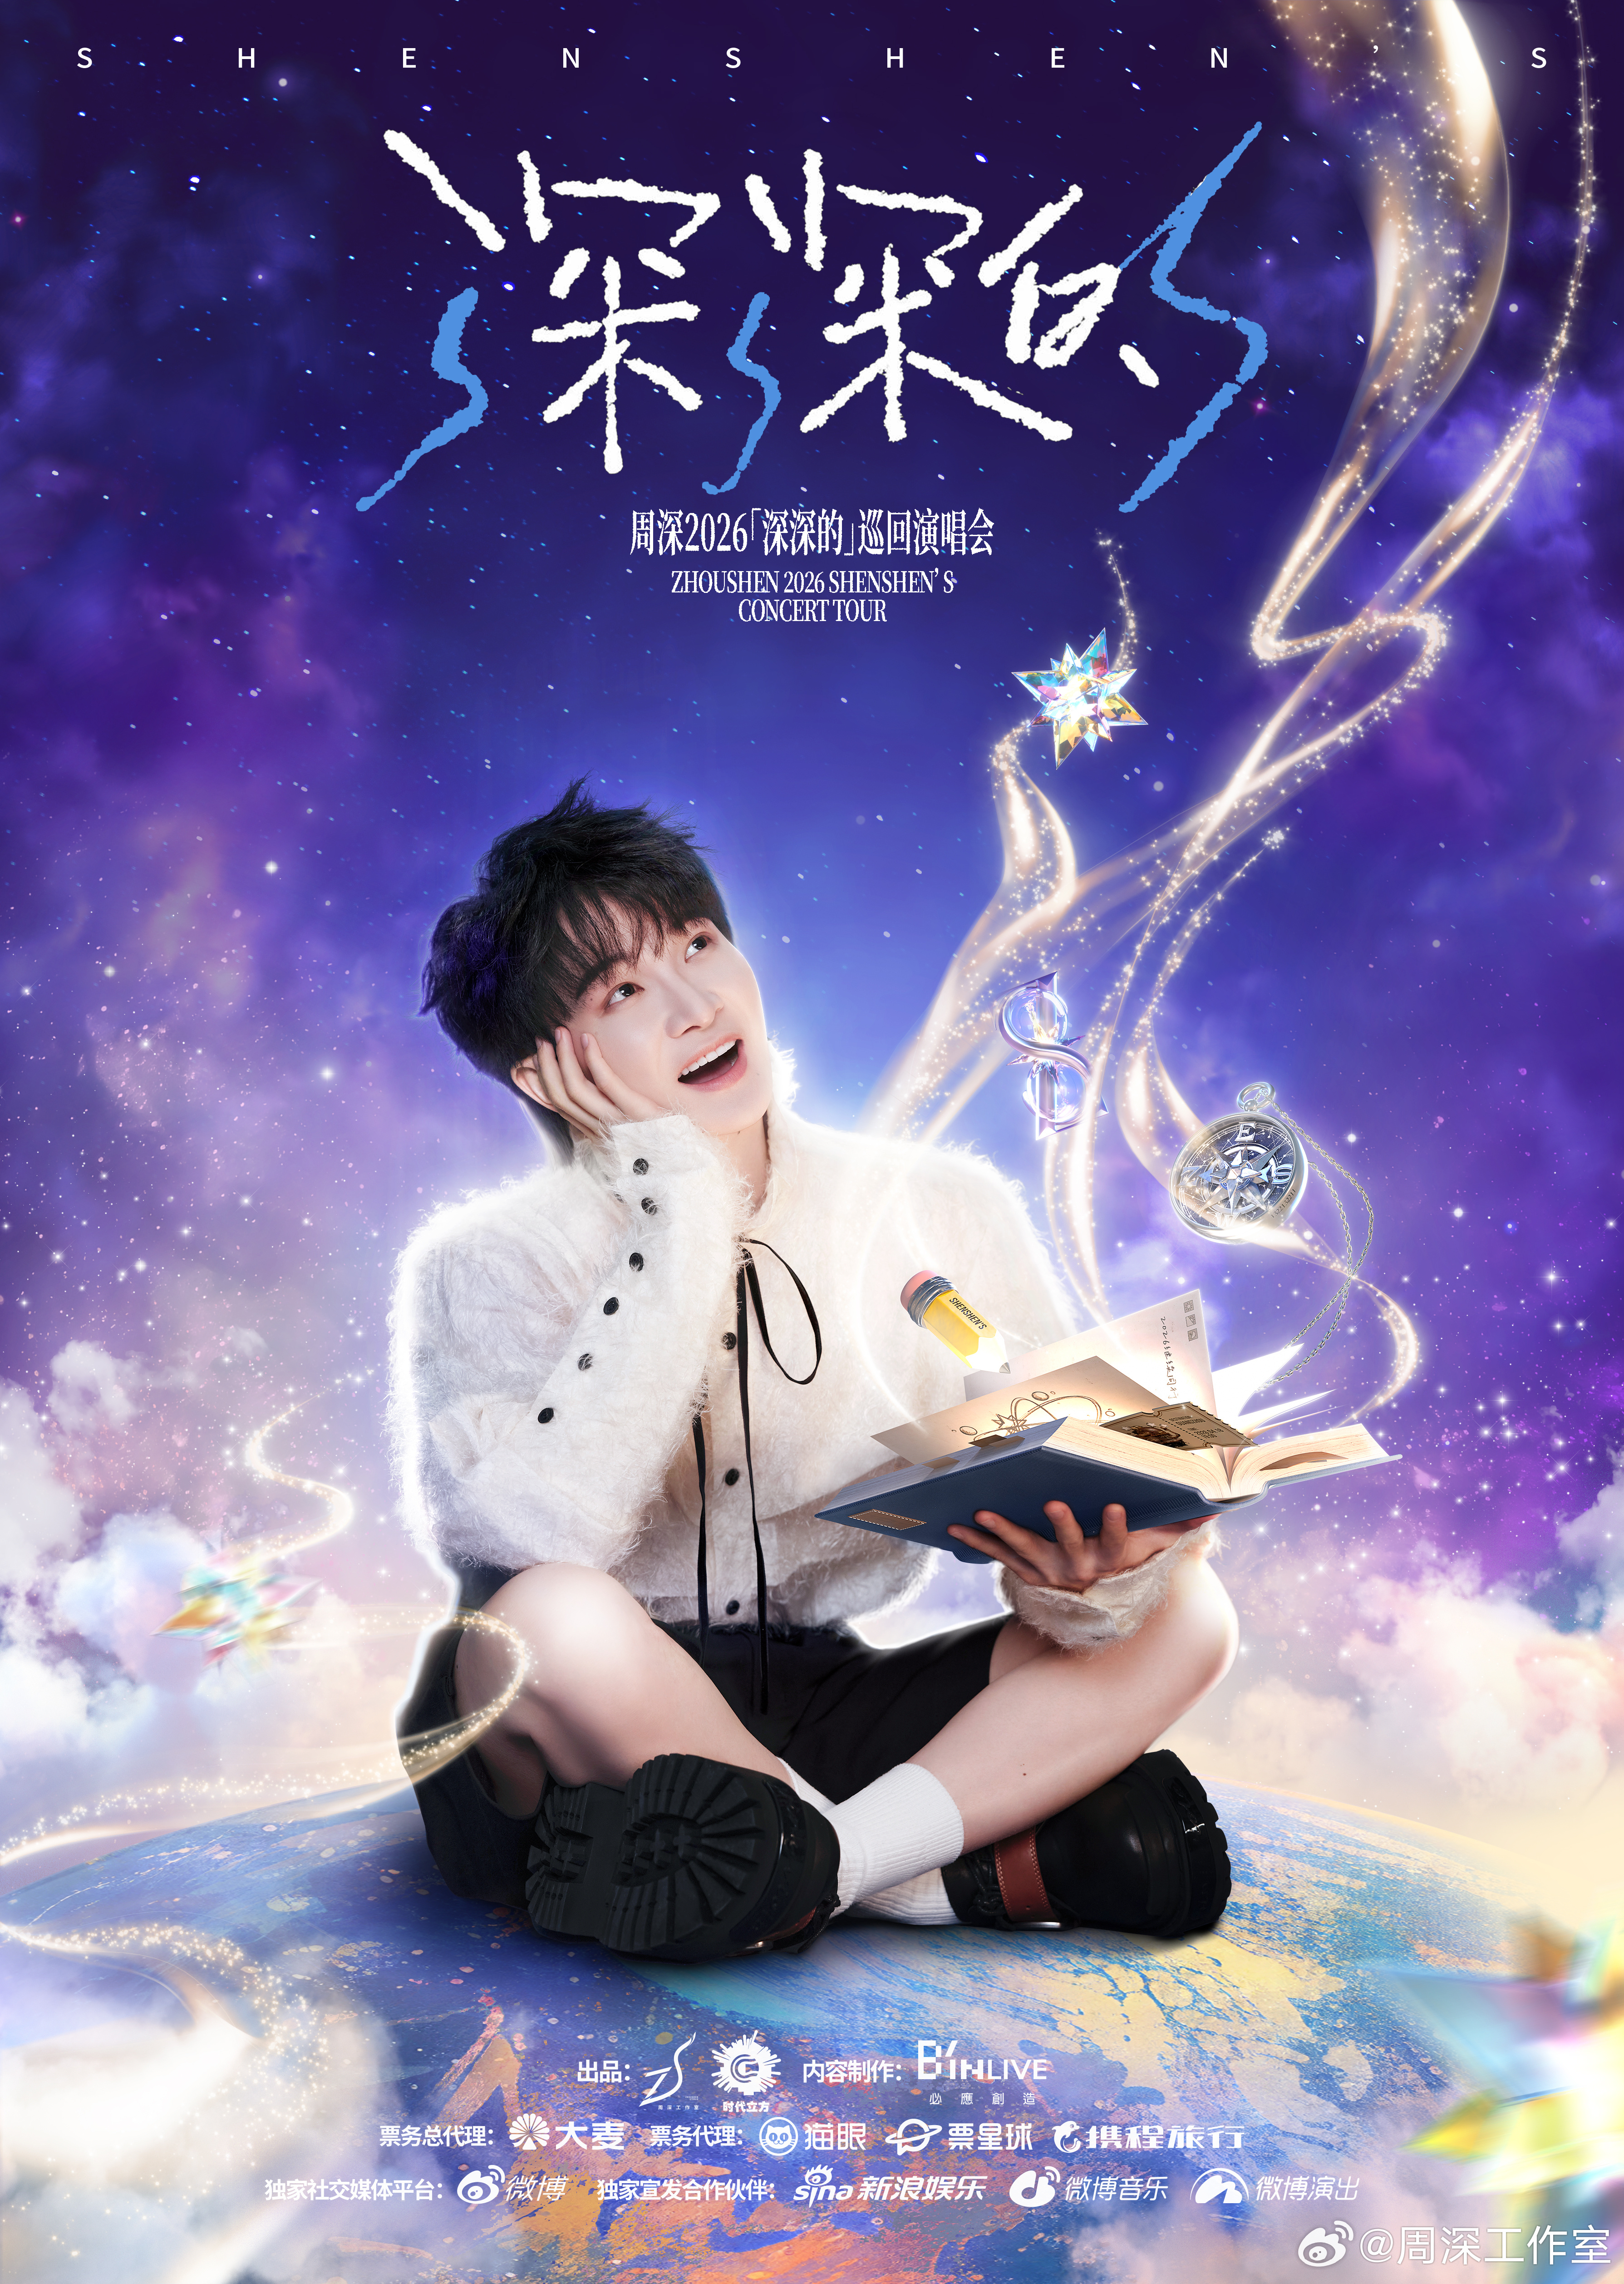
\includegraphics[width=400pt]{img/book-cover} \end{center}

\section*{关于本书}\label{about-book}


\begin{quote}
\textbf{\emph{只要你们想我的时候就可以打开那个文档。------周深}}
\end{quote}

\subsection*{1. 整理本书初衷}\label{motivation}


  在``深深的''巡演现场，深深讲了很多的话，其中，不仅有一些他首次透露的过往经历，也有他现场感人肺腑的情感表达，还有一些与生米的欢乐互动，而这一切的美好都值得被文字记录，在以后的岁月想起来的时候就翻开看一看，相信在这自带BGM的文字中，一定也有独属于你的美好回忆！你不必一口气读完此书，``\textbf{只要你们想我的时候就可以打开那个文档}''。

\subsection*{2. 本书结构}\label{book-structure}


  本书结构分为三部分，第一部分前言包括关于本书、郑重声明和致谢。第二部分主体内容为每一场``深深的''巡回演唱会深深的talking记录，每一场分为五部分，分别对应演唱会的五个部分，并附有歌单。\textbf{因为根据现场talking整理，本合集尽可能的保留原口语化说法，但部分可能有歧义的表述进行了书面化的修改，请知悉}。第三部分为巡演相关的附录，包含\hyperref[playlists]{``深深的''巡回演唱会歌单汇总}、\hyperref[appendix-gift]{``深深的''巡回演唱会彩带和伴手礼}、\hyperref[appendix-letter]{感谢信}、\hyperref[appendix-vcr]{``深深的''巡回演唱会VCR文字版}、\hyperref[related-shenshens]{``深深的''巡回演唱会其他相关视频、音频资源}。

\subsection*{3. 阅读在线版提示}\label{tips}


  本书在线版本地址为\url{https://shenshens2026.charlietalking.com}。在线版可获得更好的阅读体验------对talking重要部分进行着色区分；添加链接引用，可直接跳转。如歌曲点击歌曲名字可直接跳转至附录对应歌词，每部分结束后有深深发表的微博及工作室发布的回顾视频链接；可以发表评论并支持markdown格式；支持关键字全文搜索。

\subsection*{4. 如何为本书做贡献}\label{how-to-contribute}


  本书主体部分依据现场录音转为文字，其中可能存在一些纰漏和不足之处，欢迎大家批评指正。

\newpage

\section*{郑重声明}\label{declaration}


  1. 本书稿主体talking部分相关所有权归周深所有，\textbf{禁止用于商业盈利用途。}

  2. 本书稿\textbf{仅供生米交流学习使用}，本人承诺不会用于任何盈利活动。

  3. \textbf{本书稿仅供免费阅读，禁止读者商用、盈利，禁止无授权转载。}

  4. 本书内容为特定语境下的口述记录，请勿外延至其他语境。

  5. 本书相关图片来源``周深工作室''微博。演唱会周深发布的微博截图仅供学习交流，截图中转发、评论、点赞数目为截图时刻的数目，不代表当前数目。

  

\newpage

\section*{致谢}\label{Acknowledgments}


  首先，\textbf{感谢深深宝贝}，深深在演唱会上说过的话，既给我们带来了感动，也给我们带来了欢乐，不仅在现场给我们提供了情绪价值，也作为美好的回忆留存在我们的脑海里、我们的心里，深深，谢谢你！当然还有周深工作室的小伙伴们和为了演唱会付出的每一位工作人员，谢谢你们！

  \textbf{感谢所有给我提供过帮助的生米们}。

  \textbf{感谢喜欢本书稿的生米们}，你们的喜爱给了我非常大的动力！

  本书基于\href{https://bookdown.org/}{bookdown}框架进行撰写，感谢\href{https://yihui.org/}{Yihui}及相关开发人员开发了bookdown，大大提高了整理效率。感谢bookdown社区成员的相关文档，解决了我在整理本书稿在线版过程中遇到的技术问题，谢谢你们！

我和老婆是生米\\
2026.04.19

\chapter{2026.04.18广州场 (WIP)}\label{GuangZhou-20260418}

\begin{quote}
既然这宇宙让我们诞生了，那我们就不要再错过了，好不好？------周深
\end{quote}

\begin{figure}

{\centering 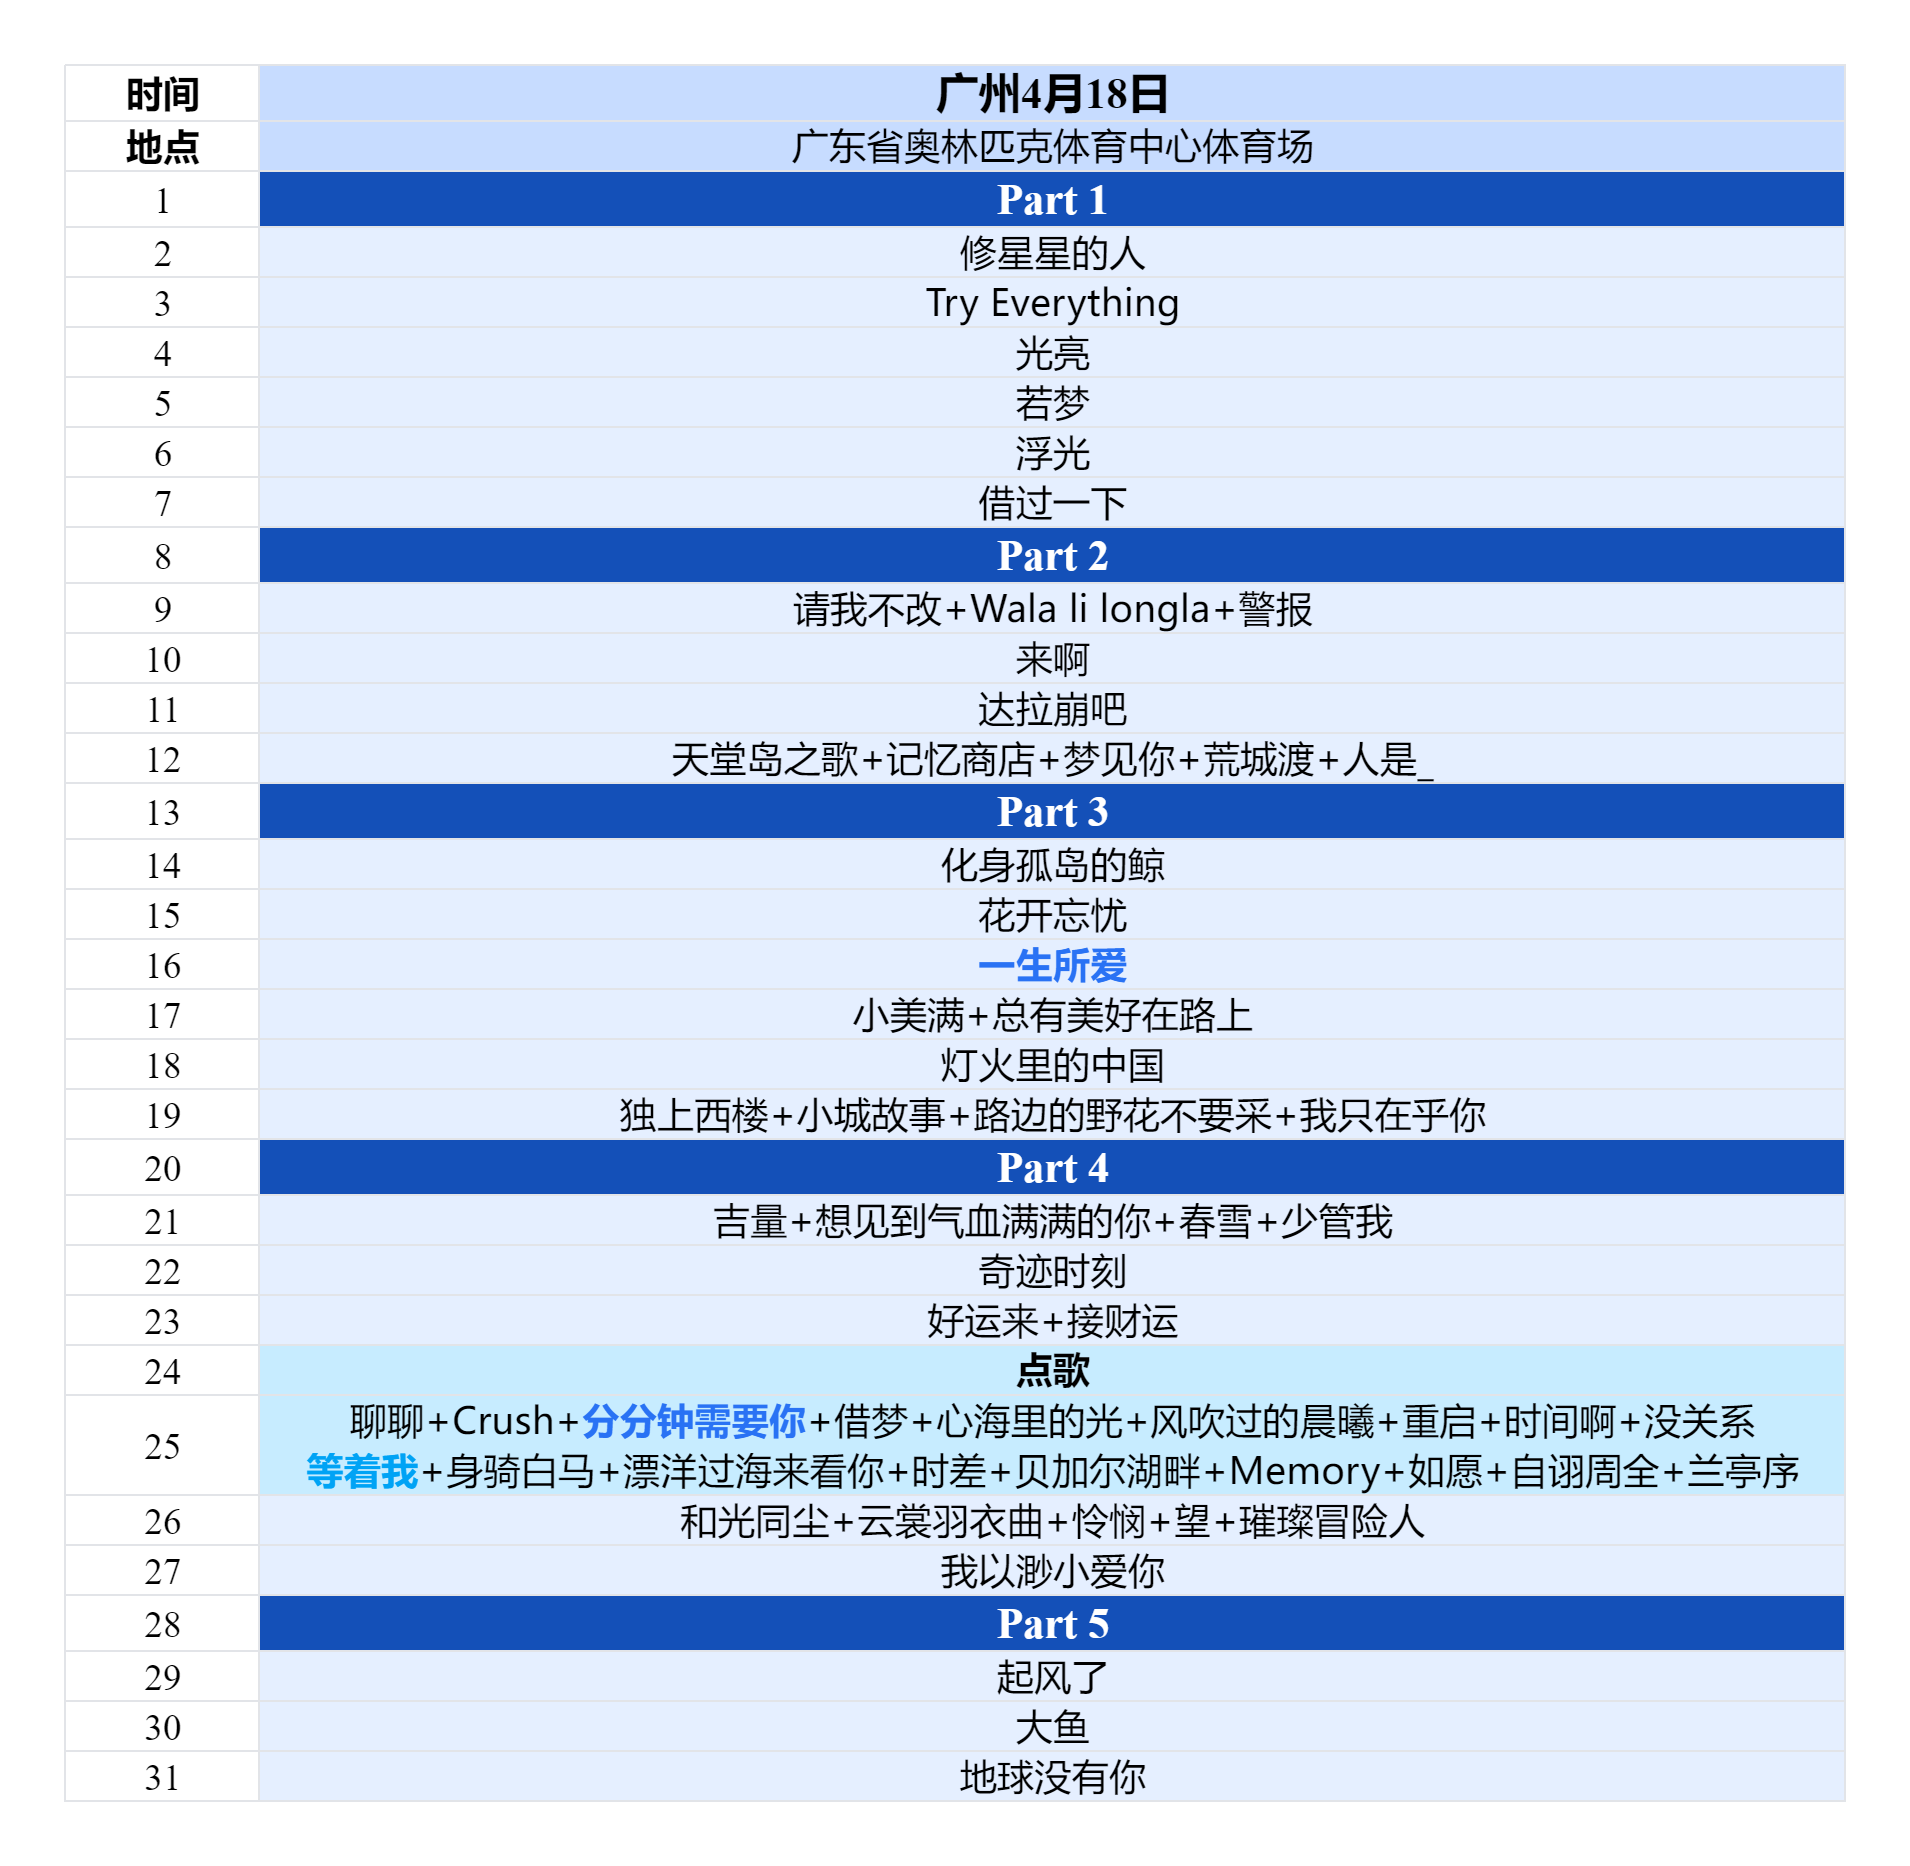
\includegraphics[width=280pt]{img/playlists/GuangZhou-20260418} 

}

\caption{2026周深“深深的”巡回演唱会2026.04.18广州场歌单}\label{fig:unnamed-chunk-5}
\end{figure}

\newpage

\section{Part1}\label{GuangZhou-20260418-part1}

\hyperref[opening-vcr]{🎥【\textbf{开场VCR}】}（VCR 正文见附录 D。VCR 结束后《修星星的人》前奏直接响起，无开场白。）

\hyperref[xiu-xing-xing-de-ren]{🎵【\textbf{修星星的人}】}（深：既然这宇宙让我诞生，想必它是要以我为证，我的情感和三十六度的体温，足以暖热即将熄灭的恒星）\textbf{\textcolor{red}{我爱你们}}。（深：是我以造物的碎屑，重塑文明的边界；是我以渺小的\ldots\ldots）让我听到广州的声音！（米：啊啊啊）（深：既然这宇宙予我重生，想必它是要让我看懂，我的基因和闪闪发光的记忆，足以照亮所有星际的永恒，永恒\ldots\ldots〔高音吟唱〕）

\hyperref[try-everything]{🎵【\textbf{Try Everything}】}既然我们已经诞生了，那就勇敢的 Try Everything 好不好？（米：好！）（深：I messed up tonight, I lost another fight, I still mess up but I'll just start again\ldots\ldots Nobody learns without getting it wrong）\ldots\ldots（深：I won't give up, no I won't give in，Till I reach the end and then I'll start again）（深：I wanna try even though I could fail）尖叫声！（米：啊啊啊）（深：Oh oh oh oh）（米：Try everything）（深：Oh oh oh oh）（米：Try everything）（深：Oh oh oh oh）（米：Try everything）。荧光棒！（米：啊啊啊）（深：I won't give up, no I won't give in）。（深：Oh oh oh oh）你们！（米：Try everything）（深：Oh oh oh oh）（米：Try everything）。

  哇！广州的朋友们你们好，我是歌手周深，你们好吗？（米：好------！）这边的朋友你们好吗？（米：好------！）中间的朋友声音有多大呢？（米：好------！）后面的朋友们呢？（米：好------！）这是我时隔六年再次来广州开演唱会，也是我第一次来广州开体育场演唱会。所以我非常非常的紧张，希望大家能再给我一点点鼓励。（米：啊啊啊）那来到广州呢，当然要说几句粤语，要说几句广东话。你们准备好了吗？（米：准备好了！）准备好听我这个就是不是很标准的粤语了吗？【粤语环节】来了哦。各位靓仔靓女，大家好我系周深，我真嘅好挂住你啊！好开心我哋在广州见面啦，你哋好唔好啊？（米：好------！）你哋知唔知我叫咩名啊？（米：周深！）我的广东话讲得\ldots\ldots（米：好好听！/很标准！）哇我们前面这位朋友直接用非常标准的普通话他说''好''！（米：哈哈）合适吗这位朋友？（米：合适！）所以真的真的很紧张。大家，你们好吗？（米：好------！）欢迎大家来到深深的巡回演唱会。这是我们又再一次开始写我们的人生日记的新的一页，你们准备好了吗？（米：准备好了！）准备好去向新的一年了吗？我说实话，我刚才在下面 stand by 的时候我已经准备想哭了，我觉得好夸张。还没开始唱就已经想哭了，因为我觉得就像前面的歌曲一样，既然宇宙让我们诞生了，那我们就不要再错过了好不好？（米：好------！）后面的朋友听到了吗？（米：听到了！）我们要一定好好的拥抱彼此好不好？（米：好------！）因为你们就是我的光亮。

\hyperref[silver-linings]{🎵【\textbf{光亮}】}好美呀！（深：海上一阵风吹起，白云涌向陆地，季风带走沙粒，四季冷暖的交替\ldots\ldots 是奔跑中突然袭来的风雨，是黑暗中一根火柴燃烧的光明\ldots\ldots 可是啊我却，愿意去相信，最渺小最微弱最柔软最无畏的你，用尽了全力，努力地去回应，再无边再无尽再无解总有一线生机，光亮你自己）（深：莫听穿林打叶声，一蓑烟雨任平生；\ldots\ldots 六百年一粟，沧海一梦）后面的朋友你们好吗？（米：好------！）（深：可是啊我却，愿意去相信\ldots\ldots）后面的 。谢谢你们来看我。大家好！（深：最无畏的你）。

\hyperref[like-a-dream]{🎵【\textbf{若梦}】}现在，你们愿意跟我一起大声唱这首歌吗？（米：愿意！）这首歌的名字叫------（米：《若梦》！）遇到你们，就像梦一样的美好。（深：浮生若梦，为欢几何；\ldots\ldots）好久不见！到你们！（深：往事）（米：往事流转在你眼眸）后面的朋友大声点！（深：一边）（米：一边遗忘，一边拼凑）（深、米：如我虔诚，合十双手）再大声------（深：唯愿）（米：你能得到拯救）四个多月之后你们怎么唱得还是这么好听！你们有想我吗？（米：有------！）。（深：情愿若梦，长久几何\ldots\ldots 愿清欢入梦，伴此身停泊）再大声！（米：往事流转 在你眼眸）。全场最大声！（米：往事流转 在你眼眸，深和声：在你眼眸，一边遗忘 一边拼凑，深和声：一边拼凑，如我虔诚 合十双手，深和声：合十双手，深：惟愿你能 得到拯救）到你们。（米：惟愿你能 得到拯救）（深：因为\ldots\ldots 你你你你\ldots\ldots）哎老师避开一下哦。〔与摄像老师互动〕（深：你\ldots\ldots 你们，周深才得到拯救。

\hyperref[floating-light]{🎵【\textbf{浮光}】}人生恍惚三万天，因为遇到了你，才值得留念。你还记得吗？（米：记得------！）那等一下会大声跟我一起唱吗？（米：会------！）（深：弹指间 破晓 蝴蝶，扇动 一场 凛冽\ldots\ldots 走进 熟悉却 陌生 的思念）你们来唱这里呢，（深：啊\ldots\ldots 米：啊\ldots\ldots）再来。（米：啊\ldots\ldots）。后面的朋友。（深：你的眼眸 装满了时间，\ldots\ldots）（深：此生如梦 愿细数流年，与你同写 沧海桑田）全场！（米：浮光掠影 重山彩云间）后面的！（米：你的伏线 穿越千百年）（深：人生不过 恍惚三万天，漫漫人间 留恋流连）。

\hyperref[excuse-me]{🎵【\textbf{借过一下}】}（深：少年扬起脸庞，前往他的月亮\ldots\ldots）少年连衣服都穿不好。（深：让我大醉一场，殿堂之上，背闲诗两三章；让我穿白衣裳，过疯人巷，去泥潭捞月光）。广州的朋友们，你们好吗？（米：好）让我听到二〇二六年第一次最大声合唱！（深：让我大醉一场）到你们！（米：殿堂之上）后面的！（米：背闲诗两三章）再来！（米：让我穿白衣裳，过风人巷）（合：去泥潭捞月光）（深：望大人们见谅）（米：提点的话）（合：我懂也不想装）再来！（深：世人寻黄金乡）后面的朋友（米：我找月亮）（合：何必偷光〔合唱句听写待核〕）再大声！（合：花谢过 路经过，你是你 我是我）再来！（合：花谢过 路经过，你是你 我是我）\textbf{\textcolor{red}{我爱你们}}！（米：啊啊啊）。你们就是我要寻找的月亮。我找到你们了。（米：啊啊啊）

\section{Part2}\label{GuangZhou-20260418-part2}

\hyperref[robot-vcr]{🎥【\textbf{机器人VCR}】}

\hyperref[brave-heart]{🎵【\textbf{请我不改}】}+\hyperref[wala-li-longla]{🎵【\textbf{Wala li longla}】}+\hyperref[jing-bao]{🎵【\textbf{警报}】}广州的朋友们！让我听到你们的声音好不好？！（米：好！！！）Wala li （米：Wala li）Wala li long（米：Wala li long）Wala li longla！（米：Wala li longla！）（深：是谁在我耳边念白，说我不配，我不够好，我必失败\ldots\ldots 绝望已经大军压境，回身却没半个人影，才看清追兵与逃兵，竟都是我自己）尖叫声（深：请我不改，我的姿态，我的爱我的痛都与生俱来；请我看开，我的存在，我的明我的暗都不必躲开；我原谅我自己，捡起遗憾拥抱无奈；我允许我放手，让我勇敢活在现在；我不等待，我不徘徊，我的笑我的泪都不再苍白，放肆盛开）尖叫声！！（米：全场尖叫）\ldots\ldots（深：请我不改，我的姿态\ldots\ldots 我的笑我的泪都不再苍白，坦荡痛快）。Wala，再来！Wala li （米：Wala li）Wala li long（米：Wala li long）Wala li longla！（米：Wala li longla！）（深：我发送警报声，血红色惊叹号，提醒你自救）爱自己！尖叫声！再来！Wala li （米：Wala li）Wala li long（米：Wala li long）Wala li longla！（米：Wala li longla！）。后面的。

  Wala li longla！（米：Wala li longla！）接下来这首这你们会唱吗？（深唱：Don't tell me lie lie lie lie lie）（米：Lie\ldots\ldots〔观众大合唱〕）这歌叫什么？（米：《来啊》！）再试一下，再学一下，不会的同学稍微学一下哦。（深唱：Don't tell me\ldots\ldots）（米：Lie\ldots\ldots〔观众大合唱〕）你们刚才那个舞挺累的，来吗？（旁：来呀！）（米：欢呼）朋友们他来不来呀？（米：来！）那就来呀！

\hyperref[lai-a]{🎵【\textbf{来啊}】}（深：我 怎么就感到，感到一不小心就落入圈套\ldots\ldots 将错就错 别拖 Let's go 随你操控 But）（深、米：Don't tell me lie lie lie lie lie，我望眼欲穿你别闪躲）再来！（深、米：Don't tell me lie lie lie lie lie）。我爱你们！再来！（深、米：Don't tell me lie lie lie lie lie，我望眼欲穿你别闪躲）（深：敢不敢直视我 Let's fall）谢谢。

  哇，上一次来这里，还是全运会的开幕式。（米：欢呼）有人记得那个舞台吗？（米：记得！）（深唱：一滴水，一滴一滴一滴一滴的水\ldots\ldots）（米：是咸的\ldots\ldots）你们居然还记得词（深唱：一汪水）你们还能记得吗？（米：一汪一汪一汪一汪的水\ldots\ldots）。（米：笑声）不要再卷我了老师们，不要再卷我了好吗？

  那接下来是我们深深的小游戏环节。（米：期待欢呼）我们的荧光棒可以自己选择自己喜欢的颜色，分别是蓝色、黄色、粉色和绿色。你们上来这是什么意思？换衣服？不同的颜色代表着不同的角色，但是我要说这句话，无论是什么颜色，你们就是人生当中最美的------（米：啊啊啊）所以，如果你想要选择达拉崩吧\ldots\ldots（米：啊啊啊）无人在意我在说什么话。（米：啊啊啊）如果选择蓝色就是达拉崩吧，黄色就是国王陛下，粉色就是公主米娅，那绿色就是\ldots\ldots（米：巨龙！！）选择好了吗？给你们五秒钟哦，五、四、三、二、一。啊\ldots\ldots 红色到底是谁？〔红色角色交代见下段〕

  真的很多。那不同的角色后面都有他的台词哦，所以我们来试一下啊。达拉崩吧！（米：我最棒！）国王陛下！（米：再说一次！）公主米娅！（米：救我啊！）恶龙！（米：嗷！嗷！）那如果是红色的话，那就\ldots\ldots 我喊\ldots\ldots（米：宝贝）那红色的话就代表他想休息一下嗓子。（米：宝贝）达拉崩吧！（米：我最棒！）国王陛下！（米：再说一次！）公主米娅！（米：救我啊！）恶龙！（米：嗷！嗷！）达拉崩吧！（米：我最棒！）国王陛下！（米：再说一次！）公主米娅！（米：救我啊！）恶龙！（米：嗷！嗷！）达拉崩吧！（米：我最棒！）国王陛下！（米：再说一次！）公主米娅！（米：救我啊！）恶龙！（米：嗷！嗷！）恶龙！（米：嗷！嗷！）恶龙！（米：嗷！嗷！）恶龙！（米：嗷！嗷！）恶龙乘以五！（米：嗷！嗷！嗷！嗷！嗷！）在广州，绝对恶龙不会饿。因为广州好吃的实在是太多了。诶，我们考验默契啊，现在我倒数三二一之后一起推荐我的美食，看一下会不会全场推荐的是同一个啊。三、二、一！（米：虾饺！）那我们等一下一起来唱这首《达拉崩吧》吧。（米：好！）

\hyperref[dalabengba]{🎵【\textbf{达拉崩吧}】}荧光棒 ！（深：很久很久以前，巨龙突然出现，带来灾难，带走了公主又消失不见\ldots\ldots 他说，陛下我叫，达拉崩吧斑得贝迪卜多比鲁翁）。荧光棒！达拉崩吧！（米：我最棒！）国王陛下！（米：再说一次！）公主米娅！（米：救我啊！）恶龙！（米：嗷！嗷！）恶龙！（米：嗷！嗷！）达拉崩吧！（米：我最棒！）国王陛下！（米：再说一次！）公主米娅！（米：救我啊！）（深：英雄达拉崩吧，骑上最快的马，带着大家的希望，从城堡里出发\ldots\ldots 闯入一座山洞，公主和可怕的巨龙，英雄拔出宝剑，巨龙说，我是昆图库塔卡提考特苏瓦西拉松）。全场的朋友，准备好了吗？（米：准备好了！）达拉崩吧！（米：我最棒！）国王陛下！（米：再说一次！）公主米娅！（米：救我啊！）恶龙！（米：嗷！嗷！）全场（深：于是，米：达拉崩吧斑得贝迪卜多比鲁翁，砍向，米：昆图库塔卡提考特苏瓦西拉松）后面的再大声。后面的再大声。达拉崩吧！（米：我最棒！）国王陛下！（米：再说一次！）公主米娅！（米：救我啊！）恶龙乘以十！（米：嗷嗷嗷嗷\ldots\ldots！），哇，你们做到了。那他的名字叫------（米：达拉崩吧斑得贝迪卜多比鲁翁！）还真是有备而来哦。这么爱念。（深：要念你来念\ldots\ldots 吧！）（米：啊啊啊）

  哇，广州是我们深深的巡回演唱会第15个城市。也就是说今天刚好是第29场。（米：哇------！）其他不是生米的朋友他们表示\ldots\ldots 然后呢？大概意思就是因为我的生日9月29，所以大家觉得9和29，和7、25，和1992，对我来说就是意义比较重大。但是我觉得最幸福的是去年、前年，哇，越说越久，前年发了一张专辑。（米：《反深代词》！）求求大家去听一下《反深代词》好不好？（米：好！）而且也在今天就是我们也算官宣，就是我们的实体专辑它终于要来了。（米：哇------！）刚才 Wala li longla 就是这张专辑当中的一个快乐密码，谁喊得越大声，快乐就来得越快。再试一下，Wala li longla！（米：Wala li longla！）那大家还记得就去年在深深的里面，是不是有人困进了蜃楼没有逃出去？诶？那么他在蜃楼当中发生了什么事情呢？大家期待吗？（米：期待！）那我们一起来看看吧。

\hyperref[haven-song]{🎵【\textbf{天堂岛之歌}】}（VCR：系统重启中\ldots\ldots 记忆读取失败\ldots\ldots 警告：检测到未知入侵者）（深：叮咚，我有一个秘密，悄悄告诉你，欢迎你来到天堂入口\ldots\ldots 叮咚，有人在看你的过去，叮咚，有人在看你的现在）生米，是你吗？（米：尖叫）（深：有个声音思念你了，你逃不掉了）。

\hyperref[the-memory-store]{🎵【\textbf{记忆商店}】}啊，我们来到了蜃楼当中的记忆商店。（米：欢呼）传说只要拥有这颗米子心〔录音听似''米字星''，写法待核〕，我们就可以购买我们最喜欢的那段记忆。我想要拥有和生米相遇的每一秒。（米：欢呼、尖叫）

\hyperref[meng-jian-ni]{🎵【\textbf{梦见你}】}（深：看着眼前，还年少的你，恍如流年从未淌过去\ldots\ldots 离别是相遇的倒影，从说问候的那天起，就有了再见的回音\ldots\ldots 我多年后还能否有幸，与你重逢在另一场梦境，但愿那时你在人海里，仍将我一眼认清）

\hyperref[huang-cheng-du]{🎵【\textbf{荒城渡}】}（深：夜色中寻觅过，当往事困住我，也盼心中生出一点萤火\ldots\ldots 断了这心魔，可原谅我，宿命中获得这解脱，重来过）（深：眼中浮沉，手中残魂，那故事斑驳荒城\ldots\ldots 想念天真，拨开心门，我宁可踏破这孤身）〔合唱句已按歌词附录校正〕

\hyperref[Humans_are_]{🎵【\textbf{人是\_}】}（深：未知摊开棋局，舍弃昨日才可破，再见了我的月光，我的蓝，我的爱\ldots\ldots 让死亡觊觎我，让恐惧亲吻我，来摧毁我深爱的一切，可仍夺不走我的选择）你们帮我！（米：让死亡觊觎我，让恐惧亲吻我，来摧毁我深爱的一切，可仍夺不走我的选择）（深：弹指间湮灭我）（米：但命运打不败活着）（深：让生命如剧烈的烟火，璀璨熄灭前也将点亮，孩童的双眸，未来的瞳孔）（米：让死亡觊觎我，让恐惧亲吻我\ldots\ldots 我们依然前行，没有光指引）〔大合唱段落〕（深：我开始相信，让时空笑忘我，你无需记得我）〔结尾句听写待核〕。

\section{Part3}\label{GuangZhou-20260418-part3}

\hyperref[music-animations-vcr]{🎥【\textbf{音乐动画VCR}】}（VCR 正文见附录 D。与常州场不同，本场动画结尾有一句旁白------``如果遇到了你，我们一定可以好好享受现在。挣脱才能定义的束缚，对不对？''〔听写待核，疑为''挣脱人设定的束缚''〕）（米：对！）〔VCR 后为纯音乐过场，无 talking〕

\hyperref[The-whale-who-became-an-island]{🎵【\textbf{化身孤岛的鲸}】}你们唱给我听好不好？（米：好------！）（深：我是只化身孤岛的蓝鲸，有着最巨大的身影，鱼虾在身侧穿行，也有飞鸟在背上停\ldots\ldots 我爱地中海的天晴，爱西伯利亚的雪景，爱万丈高空的鹰，爱肚皮下的藻荇，我在尽心尽力地多情，直到那一天）到你们！（米：你的衣衫破旧，而歌声却温柔，陪我漫无目的的四处漂流）谢谢你们接住了我。（深：我的背脊如荒丘，而你却微笑摆首，把它当成整个宇宙）（米：你与太阳挥手，也同海鸥问候，陪我爱天爱地的四处风流）（深：只是遗憾你终究，无法躺在我胸口，欣赏夜空最辽阔的不朽，把星子放入眸）（米：欢呼、喝彩）（深：我是只化身孤岛的蓝鲸\ldots\ldots 未有过滚烫心情，所以也未觉大洋正中）到你们！（米：我有着太冷太清的天性）后面的朋友！（米：对天上的她动过情）全场最大声！（米：有多么安静）再来！（米：你的衣衫破旧，而歌声却温柔，陪我漫无目的的四处漂流）（深：我的背脊如荒丘\ldots\ldots 把星子放入眸）（深：你的指尖轻柔，抚摸过我所有，风浪冲撞出的丑陋疮口；你眼中有春与秋，胜过我见过爱过的一切山川与河流；曾以为我肩头是那么的宽厚，足够撑起海底那座琼楼，而在你到来之后，它显得如此清瘦，我想给你能奔跑的岸头）（米：加油！〔零星喊声〕）

  （深：多少个墙头）（米：没有！）真的没有吗？（米：没有！）我解释一下，墙头的意思就是说，每当要问，哎，你们喜欢哪个歌手啊，他们会说------（米：周深！）然后他会追问，啊？只喜欢周深吗？（米：是的！）你看，他们虽然嘴上说着只喜欢周深，但是有很多墙头，所以墙头的意思就是说\ldots\ldots（米：没有！）（深：多少个墙头）（米：没有墙头！）无论如何，（深：你们都是我的国王和皇后）〔``皇后''写法待核，1108场作''王后''〕谢谢你们来看我。

\hyperref[Blossoms-that-forget-sorrow]{🎵【\textbf{花开忘忧}】}我们来广州看你咯。（米：欢呼）你有好好照顾好自己吗？（米：有！）真的有吗？（米：有！）（深：巷子口买了花，穿过沿街红墙青瓦\ldots\ldots 一件遗憾的事就喝一碗汤，庭院深深，秋叶飘落）（深：我们苍老的时候就回到小时候，采青梅用来酿酒你不许偷着喝，穿朴素的衣裳牵着那衣袖，捡了小猫名为苍狗）我说，说什么？（米：你好啊！）你们好吗？（米：好！）（深：这是给你的花，花的名字叫忘忧草，它说时光汹涌如水上烟波，别走远了一起回家）（米：欢呼、掌声）我们来广州看你咯。不要浪费我们这一生的相遇好不好？（米：好！）（深：我们苍老的时候就回到小时候）到你们！（米：采青梅用来酿酒你不许偷着喝）（深：穿朴素的衣裳牵着那衣袖）到你们！（米：捡了小猫名为苍狗）再来。（深：我们睡去的时候像孩子无忧愁）（米：在梦里做个梦，看见你我都老了）（深：那永恒没骗我，离散也没有）（米：这份爱只是活在另外时空）（深：如果每一声再见会开启一个新的空间）（米：每做一个梦是时空偶尔的重叠）（深：你好吗，离开的人啊，请帮我相爱到剧终）（深：忘忧草开着花，你在月光下不说话，一件遗憾的事就喝一杯茶，庭院深深，秋叶飘落）既然这宇宙让我们诞生，就请我们好好的\ldots\ldots 拥抱彼此好不好？（米：好！）不要浪费这一次相遇，好不好？（米：好！）因为，我们心中一直思念的那个人，他一定看得到，听得到，对不对？（米：对！）花开忘忧。（米：愿你无忧！）花开忘忧。（米：愿你无忧！）谢谢你们来看我哦。（米：谢谢周深！）

  哇，我真的好开心来广州同你哋见面啊。虽然咧我哋广东话咧真系好差。但系，我为什么一直要勉强自己说广东话？但是，好听的粤语歌实在是太多了。所以在选的时候我都觉得哇，恨不得选三十首。那如果选三十首，周深唱什么？那大家有听过周深的歌吗？（米：有！）我也就只敢在你们面前问一下了。后面的朋友你们听过吗？（米：听过！）所以今天这首啊，是我一直都非常喜欢，大家在\ldots\ldots 在大家的心中也非常经典的一首歌，叫做《一生所爱》。很多爱，很多相遇，不要等过了五百年后才珍惜，才后悔。因为我们可以拥有的最好的，就是现在。我看到了你，你听到了我，你们就是我的一生所爱。你们会唱吗？（米：会！）那等一下后面有一段你们最大声唱好不好？（米：好！）后面的朋友好不好？（米：好！）

\hyperref[yi-sheng-suo-ai]{🎵【\textbf{一生所爱}】}（深：从前现在过去了再不来，红红落叶长埋尘土内；开始终结总是没变改，天边的你飘泊白云外；苦海翻起爱恨，在世间难逃避命运；相亲竟不可接近，或我应该相信是缘分）（深：情人别后永远再不来，无言独坐放眼尘世外；鲜花虽会凋谢，但会再开；一生所爱隐约，在白云外）全场最大声！（深：苦海翻起爱恨）（米：苦海翻起爱恨）（深：在世间难逃避命运）（米：在世间难逃避命运）（深：相亲竟不可接近）（米：相亲竟不可接近）全场最大声！再来！（深：苦海，翻起爱恨）（深：在世间，难逃避命运）（深：相亲，竟不可接近）（深：或我应该相信是缘分）你们！（米：苦海翻起爱恨，在世间难逃避命运，相亲竟不可接近，或我应该相信是缘分）（深：或我应该相信是缘分）哎呀你们这么好，不愧是我的一生所爱。听到最大的声音好不好？（米：好！！！）后面的朋友，准备好了吗？（米：准备好了！）

\hyperref[simple-bliss]{🎵【\textbf{小美满}】}那这首歌，你们会唱吗？（米：会！！！）（深、米：没什么大愿望，没有什么事要赶；看见路口红灯一直闪，它像眨眼的小太阳；乌云还挺大胆，顶在头上吹不散，我抓在手里捏成棉花糖，什么烦恼不能忘）大声点！（深、米：既然是路一定有转弯，哪个风景都漂亮，揉揉疲惫的眼睛停下来看一看，美好简单）全场最大声！（深、米：你看小狗在叫，树叶会笑，风声在呢喃）大声点！（深、米：不如好好欣赏一秒迷迷糊糊的浪漫）这边的朋友大声唱好不好？（米：好！！！）（深、米：笑一笑就灿烂，唱一句歌就舒展，收集一点一滴小美满，都是幸福的花样，没道理的开朗）然后呢？（深、米：打扮平凡的日常，找到自己最合身的衣裳，只要自己够喜欢，至少还有温柔的眼光，还在夜里看月亮，心情铺得再满也要留一扇天窗，岁月很长）再大声！（深、米：你看小狗在叫，树叶会笑，风声在呢喃）后面的！（深、米：不如好好欣赏一秒迷迷糊糊的浪漫）亲爱的朋友们，让我们一起再一次在深深的〔巡回演唱会当中〕许愿好不好？〔原句听写待核〕（米：好！！！）谢谢你们愿意来和我见面。我们这里有一棵许愿树，像我这样，闭上眼睛，想好心中的愿望。然后我会倒数三个数字，三、二、一\ldots\ldots 愿望就会出现在许愿树上哦。现场的每一个最可爱的你，请相信相信的力量。相信你自己的力量。现在想好你心中想要许的愿望吧。想想哎，生日的时候，一直想要许什么愿望呢？嗯，哦对了。在深深的巡回演唱会当中，只能够许关于你自己的愿望哦。大家闭上眼睛，许愿啦！想想，是不是很久没有跟自己说一句，哇，你真的很了不起哦。你身上这些经历、这些挑战，放在别人身上，真的他不一定能撑下来哦。是不是忘记给自己一个拥抱啊？是不是没有跟自己说过一句，我真的应该好好的爱你，好好的喜欢你？现在，睁开眼睛，三、二、一！（米：欢呼、尖叫）（深：笑就好，哭也好，今天就是明天最好的陪伴）到你们唱！（米：自己就是自己最好的陪伴）（深唱：你们都是周深最好的陪伴）〔现场改词，听写待核〕（米：欢呼、尖叫）好好照顾好自己好吗？（米：好------！）相信我，爱自己一定是终身浪漫的开始哦！（米：欢呼）

\hyperref[zong-you-mei-hao-zai-lu-shang]{🎵【\textbf{总有美好在路上}】}（深：花在开，云在飘，笑容在脸上，我们向前方一路向阳）（米：我们向前跑，一路向阳〔合唱句听写待核〕）（深：亲爱的你，在路上慢慢逛，看一看太阳）（深：今天过去，要到明天看看天气会怎样，阴或晴朗，故事都慢慢赏）（深：抬头发现，光一直在身上）〔合唱句听写待核〕因为你们就是那道光啊！（米：欢呼、尖叫）谢谢你们！（米：谢谢深深！）

\hyperref[deng-huo-li-de-zhong-guo]{🎵【\textbf{灯火里的中国}】}（深：都市的街巷已灯影婆娑，社区暖暖流淌的欢乐，远山的村落火苗闪烁，渐渐明亮小康的思索\ldots\ldots 灯火里的中国青春婀娜，灯火里的中国胸怀辽阔，灯火漫卷的万里山河，初心换回了百年承诺）你们准备好唱了吗？（米：准备好了！）我们的朋友，等一下让我听到你的声音好不好？（深：归港的船帆从灯塔掠过，追梦脚步月下交错，广场焰火在节日诉说，星空升腾时代的巍峨）全场最大声！（米：灯火里的中国，青春婀娜）大声点！（米：灯火里的中国，胸怀辽阔）再来！（米：灯火灿烂的中国梦）后面呢？（米：灯火荡漾着心中的歌）（米：灯火里的中国，青春婀娜，灯火里的中国，胸怀辽阔，灯火灿烂的中国梦，灯火荡漾着心中的歌）全场！（米：灯火里的中国，青春婀娜）再大声！（米：灯火里的中国，胸怀辽阔，灯火灿烂的中国梦，灯火荡漾着心中的歌）再大声！（米：灯火荡漾着心中的歌）（深：心中\ldots\ldots 的歌\ldots\ldots〔高音拖长〕）。

  广州的朋友们唱得好啊！（米：欢呼）给自己一点点鼓励！呜呼！呜！现在的''哦''明显比前面的''哦''小声很多，看来《灯火里的中国》挺难唱的哦。唱够了没有？（米：没有！）哦，唱够了没有？下面的朋友呢？（米：没有！）如果嗓子不舒服，那要记得------（米：喝水！）又到了我在演唱会宣传我担的时候啦。你们记得，就是我担是谁吗？（米：邓丽君！）你们还记得我是谁吗？（米：周深！）哦，知道自己是来看的周深的演唱会哈？（米：知道！）知道哈，好的。我也希望自己可以成为像邓丽君女士这样的歌手，有好多好多作品可以去陪伴大家。去，可以大家每次听到首歌都是想起很多很多美好的回忆。但是，也像刚才我们那个小小的片段一样，告诉你，不要被任何的回忆困住原地。不要被任何的记忆困在原地哦。因为我们有掌控时间的魔法，就是珍惜当下，对不对？（米：对！）而且，我担的歌里面有我们今年巡回演唱会的主题哦。我们一起来找一下啊。（深唱：无言独上西楼\ldots\ldots）唱错了。要不就先唱这个吧。（深唱：你问我爱你有多深）（米：我爱你有几分）（深唱：轻轻的一个吻）（深：他是不是最近的词一直在那个脑袋里面翻覆，重来啊）〔口播自嘲串词〕（深唱：轻轻的一个吻）你们？（米：已经打动我的心）接下来这三个字。（米：深深的一段情）（深唱：叫我思念到如今）那等一下如果有你会唱的歌跟我一起唱好不好？（米：好！）一起哦。（米：好！）

🎵【\textbf{邓丽君组曲}】

\hyperref[du-shang-xi-lou]{🎵【\textbf{独上西楼}】}（深：无言独上西楼，月如钩，寂寞梧桐，深院锁清秋；剪不断，理还乱，是离愁）（米：别是一般滋味在心头！）（深：别有一番滋味在心头）

\hyperref[xiao-cheng-gu-shi]{🎵【\textbf{小城故事}】}这首歌会唱吗？（米：会！）最大声！（深：小城故事多）到你们！（米：充满喜和乐）（深：若是你到小城来）（米：收获特别多）最大声！（米：看似一幅画）后面的！（米：听像一首歌）（深：人生境界真善美）（米：这里已包括）（深：谈的谈，说的说）你们墙头真的多！（米：没有！）（深：请你的朋友一起来）（米：小城来做客）到你们！（米：请你的朋友一起来）来哪里？（米：小城来做客）

\hyperref[donot-pick-the-roadside-flowers]{🎵【\textbf{路边的野花不要采}】}让我听到你最大的声音好不好啊？（深：送你送到小村外）（米：有句话儿要交代）（深：虽然已经是百花开）旁边的人听好咯！（深：路边的野花）它怎么啦？（米：你不要采）好像有的人会听到当没听到对不对啊？（深：记着我的情，记着我的爱）（米：记着有我天天在等待）（深：我在等着你回来）（米：千万不要把我来忘怀，千万不要把我来忘怀，千万不要把\ldots\ldots）什么？（米：我忘怀！）

\hyperref[I-only-care-about-you]{🎵【\textbf{我只在乎你}】}谢谢你们来看我哦。谢谢你们陪我一起唱歌。陪我打开我们的时间胶囊。我不敢想象如果没有遇到你，我的人生会是什么样的呢。（深：如果没有遇见你）（米：我将会是在哪里）（深：日子过得怎么样）（米：人生是否要珍惜）（深：也许认识某一人）（米：过着平凡的日子）（深：不知道会不会）（米：也有爱情甜如蜜）全场！（深：任时光匆匆流去）（米：我只在乎你）（深：心甘情愿感染你的气息）最大声！（米：人生几何能够得到知己）（深：失去生命的力量也不可惜，所以我求求你）（米：别让我离开你）（深：除了你我不能感到一丝丝情意）全场最大声！（深：任时光匆匆流去）（米：我只在乎你）（深：心甘情愿感染你的气息）

\section{Part4}\label{GuangZhou-20260418-part4}

\hyperref[mask-vcr]{🎥【\textbf{面具VCR}】}（VCR 正文见附录 D。开篇日期行本场为''2026年4月18日，广州''，其余与附录 D 一致，含''我就戴上了一个幺蛾子面具，还有一个背包客面具''〔蒙面唱将猜猜猜面具梗〕。）

（米：对！！！）〔回应 VCR 结尾''你说，对吗？``〕没听到哦。（米：对！！！）好吗？（米：对！！！）

\hyperref[ji-liang]{🎵【\textbf{吉量}】}（深：羲和车上金铃铛）（米：叮当，叮当）你们会唱吗？（米：会！！！）（深：望舒驾后银尾巴，摇摇晃晃）你们？（米：哇！！！）（深：弱水岸边唤吉量，吉量吉量）（米：叮叮当当，叮叮叮叮当当）你们好吗？（米：好！！！）（深：九天之上飘来一朵雪花，原来是我的英俊的小马，金色星星在它眼里安家，祝融手持火种编织了它的发）〔已按歌词附录校正，录音听写偏差见文末备注〕（深：朱唇染尽火种，燃起了她的发〔听写待核〕；我的小马一天一天长大，穿过凛冬和最沸腾的夏）会唱的跟我一起，注意安全！（米：高高山上赶牛羊，叮当叮当；风在浪里脚印长，沙沙荡荡；千户树下唤吉量，吉量吉量；叮叮当当，叮叮叮叮当当）〔合唱段听写待核〕你们好漂亮啊！（深：吉量，我勇敢的向往，当人间需要照亮，请你垂下缰；吉量，树顶上那轮太阳，燃烧无尽的光，温暖了我身旁）后面的朋友！（米：谁在车上听铃铛，叮当叮当〔合唱句听写待核〕）让我听到你们的声音！（米：高高山上赶牛羊，叮当叮当）荧光棒！

  回答问题！你是谁？你是自己的------（米：宝贝！）宝贝！（深：有时候感觉自己多珍贵，还会有更好的等着你，还有好多梦在飞，还要给自己一个新的机会；要早起早睡，别那么累，做好气血满满的准备）我看到你了哦！（深：再疼再冷再怕的时候，请你一定记得，我永远会是你停靠的选择）你好吗？（深：我有梦可追，勇气可归，举起热情满满的奖杯，那时的你，灿烂的你，无惧也无畏）你是谁？你是自己的------（米：宝贝！）你们是我的宝贝！广州的朋友，诶这边的声音有多大让我听一下？那这边的朋友呢？哦？那我们的小火车继续出发咯！

\hyperref[xiang-jian-dao-qi-xue-man-man-de-ni]{🎵【\textbf{想见到气血满满的你}】}（接上首连唱，两首之间无 talking）

\hyperref[chun-xue]{🎵【\textbf{春雪}】}（深：白是梦境的泥土，白是回忆的发束，有些记忆依然自反复，练就成我们的天赋，也不免在这一生寒苦；冰是血色的礼物，却努力重来时的温度，融化难以碰触，沿着心底泛流关注，让面孔化作纪念）〔唱词已按歌词附录校正，录音听写偏差见文末备注〕你们好吗？（米：好！）谢谢你们！注意安全！（深：我想在冬夜雪地与你追逐，你却落在早春中的一棵树；一次错过不算错误，错在来不及，看清楚你的面目我就交出全部）到你们！（米：我想在冬夜雪地与你追逐）后面的！（米：你却落在早春中的一棵树）（深、米：雪花开在冬夜深处蔓延，蔓延到一个危险的春天；春天蚕食消融目空一切，一切啊那曾是我的世界）\ldots\ldots（深、米：我在原地守护我的体面，春天再见，春天再见；我还在冬夜雪地里等日出，你落满早春枝叶宣判我输；趁着交迫还没结束，在这一条必经之路，我下慢了脚步，陪你庆祝）

\hyperref[watch-ur-manners]{🎵【\textbf{少管我}】}嘿！少管我！（米：欢呼、尖叫）在做自己的人生路上，在不打扰别人的前提下，遇到烦恼就轻声说一句：嘿！（米：嘿！少管我！）（深：无数麻烦是想要无聊的理由，把沉重身体传送到热带气候，脑袋放空，吹吹海风，用一场远行当做逃离的方舟；做生活困兽不如去浪漫宇宙）你们好吗？（米：好------！）（深、米：我想我可以，抓住风中飘散的花，不介意坠入水星或是泥巴，跟现在握手拥抱道别出发，别停下）（深、米：我想我成为阳光蔷薇飞鸟盛夏，或成为昆虫砂砾一片雪花）你好吗？（米：好------！）会唱的一起！（深、米：我想我可以，抓住风中飘散的花）三二一！嘿！（米：嘿！少管我！）这边！五四三二一！嘿！（米：嘿！少管我！）再来！嘿！（米：嘿！少管我！）呜------！五四三二一！嘿！（米：嘿！少管我！）（深、米：我想我可以，抓住风中飘散的花\ldots\ldots 我想我成为阳光蔷薇飞鸟盛夏，或成为昆虫砂砾一片雪花）

  你们每个人创造的奇迹，你们要记得好不好？（米：好！）后面的朋友听到了吗？（米：听到了！）那边的朋友听到了吗？（米：听到了！）被你们听到和遇到，每一秒都是奇迹时刻哟！（米：欢呼、尖叫）

\hyperref[miracle-moment]{🎵【\textbf{奇迹时刻}】}（深：藏进发光的恒星，穿梭时空的王牌，每个瞬息都能将苦涩一键更改\ldots\ldots I wanna see my way in the starlight，奇迹时刻等你一起来，开启夺目现在；We gonna change the fate never deny，以无数个渺小的光彩，就能照亮无穷未来）〔唱词已按歌词附录校正〕哇，你们自信！（米：欢呼）（深：就算我们彼此信赖，就能将命运更改；以最大纯朴力和热爱，就能一起创造姿态）。

  我又要开始变魔术啦！（米：尖叫、欢呼）不好意思我先笑一下。经过了四个月的练习\ldots\ldots 魔术没有什么进步。但是大家会给我鼓励吗？（米：会！）大家看一下啊，这是一个\ldots\ldots 这是木头对不对？是个方块对不对？（米：对！）我这样把它推进去。然后这里插上一个门栓，它没办法掉出来对不对？（米：对！）诶，但是如果遇到了你们，那就不一样了。我们来看啊，这还是那个木头，还是那个方块对不对？（米：对！）还是像刚刚把它卡进去对不对？（米：对！）还是这个木梢，把它插上去对不对？（米：对！）那你们觉得我能不能够隔空把它掉下来呢？给我三个数字，三！（米：二！一！）（米：惊呼：哇！）（深唱：这是给你的花，花的名字叫忘忧草〔变魔术中唱《花开忘忧》句〕）〔魔术道具与唱句对应关系听写待核〕刚变魔术厉不厉害？（米：厉害！）这是一朵蓝玫瑰。怎么变的？三、二、一！（米：欢呼：哇！）再看哦！（米：欢呼：哇！）厉不厉害？再盯着这个球啊。没有啦！（米：全场爆笑、掌声雷动）这边也没有啦！（笑声）哎呀我不行了，笑死我了。那你们看懂这个魔术了吗？（观众：没有/没看懂）没有看懂就对了，因为我也没有看懂。但是，我只想问，好运来了的话，接不接？（米：接！！！）大声点，好运来了接不接？（米：接！！！）刚才的魔术，结束，你们接不接？（米：接！！！）

\hyperref[good-fortune-comes]{🎵【\textbf{好运来}】}（深、米：好运来祝你好运来，好运带来了喜和爱，好运来我们好运来，迎着好运兴旺发达通四海）（深：叠个千纸鹤，再系个红飘带，愿善良的人们天天好运来\ldots\ldots 你凤舞太平年，你龙腾新时代，你幸福的家园迎来百花盛开）全场最大声！（深、米：好运来祝你好运来）大声点！（深、米：好运带来了喜和爱，好运来我们好运来，迎着好运兴旺发达通四海）好运来了接不接？（米：接！！！）等下唱的再大声一点好不好？（米：好！！！）（深：叠个千纸鹤，再系个红飘带，愿善良的人们天天好运来\ldots\ldots）最大声！（深、米：好运来祝你好运来）再大声！（深、米：好运带来了喜和爱，好运来我们好运来，迎着好运兴旺发达通四海）这边的再大声！（深、米：好运来祝你好运来，好运带来了喜和爱）再大声！（深、米：好运来我们好运来，迎着好运兴旺发达通四海）广州的朋友们，新的一天祝福全都有，大家跟我一起大声的接，好不好？（米：好！！！）

\hyperref[jie-cai-yun]{🎵【\textbf{接财运}】}要最大声哦，我们一起，接平安！（米：接平安！）接平安！（米：接平安！）接幸福呢你们？（米：接幸福！）接健康大声！（米：接健康！）接财运！（米：接财运！）全部来！（深、米：接个好运来，接个福气来，接个财神开开心心到我家里来，接个财运来，小财大财，我接我接，我接金山银海）〔唱词已按歌词附录校正，录音听写偏差见文末备注〕（深、米：好运来，我接个好精彩；好运来，我接个好运来，我接个福气来，我接个大口袋）广州的朋友，恭喜发财！（米：欢呼尖叫）接不接？（米：接！！！）

【\textbf{点歌环节}】
  谢谢。那接下来，到我们的点歌环节。（米：全场欢呼尖叫）好运来接不接？（米：接！！！）全场帮我倒数五个数字好不好？（观众：好！/五！四！\ldots\ldots）你们是累了吗？（观众：没有！）广州的朋友们你们还好吗？（米：好！！！）倒数五个数字，五！（米：四！三！二！一！）停！哦哦在那里，没事没事。好，Hello！老师给他一点光，光来。Hello！（金雨：深深你好！）哇，你好你好，怎么称呼您？（金雨：我叫金雨。）金雨是吗？哦你好你好，来自哪里的朋友？（金雨：我是广州的。）哦，广州本地的？（金雨：我在这上学。）哦在这里读书，今年大几？（金雨：今年博四。）（米：欢呼、惊叹）哇，也是毕业。想过自己会没礼貌和冒犯，没想到这么没礼貌这么冒犯，对不起。〔玩笑：把博士说成''大几''〕你看着太年轻了。不过博四是不是现在大家都越来越有朝气，博四什么专业的呀？（金雨：临床医学。）（米：欢呼、掌声）辛苦了。学医生真的很辛苦，谢谢你，谢谢你。哦那旁边这位摆件是\ldots\ldots 这边是一起来的吗？（金雨：对，他是我对象。）哦，怎么称呼他？（金雨：他叫小武。）确定就是不让他自己介绍一下自己？（武勋：我叫武勋。）武勋，哦和金雨，哦，他也是博士？（金雨：没有，他本科。）（米：大笑）哇，我刚才脑子里转了一圈，我圆不回去哎。没事，学到了好本事就是本事。所以你是什么专业的，武勋？（武勋：计算机。）计算机，哦，那现在是不是在就是往AI那方向在延延展？（武勋：啊对了对了。）哦，你会，你如果就是设计出最厉害的AI软件，你最想最想做的事情是什么？（武勋：做游戏。）也可以，就是可以帮大家就是去平时压力大的时候去帮助他们嘛。好，让我们目光回到我们的金雨女士。你好。（金雨：你给他的游戏唱过歌。）（米：欢呼）什么什么什么？（金雨：你给他做的游戏唱过歌。）王者荣耀吗？（金雨：是海上蝶。）（米：欢呼）哦谢谢，好有缘分哦。好，我现在只给王者荣耀唱歌。就希望就是可以在峡谷当中陪伴大家，用音乐陪伴陪伴大家。你第一次听我的歌是哪首歌啊？（金雨：漂洋过海来看你。）哦是我在舞台上唱的那个那个版本还是就是只是音频文件？（金雨：呃音频。）那你听我歌听很久了哎。（金雨：对，我本科就在听。）（米：大笑）好啦知道了，你从本科听到了博士。博四，博士，博士，四。那我们今天来点歌吧，点歌今天就是你可以选择蓝色的笔或者是粉色的笔。蓝色的笔就是这边的九首，粉色的笔就是这边的九首。你可以写一个祝福也好，或者你最想说的话写在便签上。然后下一场的时候呢，你你们的照片和你写的那个话就会出现在我们后面的背景上哦。所以就是祝福给我们每一个听到我的朋友和美好的朋友的好不好？然后但是我们先点歌好不好？（金雨：好。）谢谢你谢谢你。你你老家是哪里的？（金雨：湖南。）湖南的啊？湖南哪里的？（金雨：永州。）哦，那你在广州读博四，你会说粤语吗？（金雨：我都唔知啊〔我都不知道啊〕。）（米：大笑）行，点歌吧。蓝色和粉色。（金雨：分分钟需要你。）（米：笑声）思考很严严谨。谢谢你非常珍惜我们这次点歌机会，很开心。（金雨：那我点分分钟需要\ldots\ldots）（米：欢呼、尖叫）哇她这么开心。好，那等一下就是我们的工作人员会给你蓝色的笔，然后给你写出你想要给我们的祝福或者怎么样好不好？那先留下你和武先生在这里的照片，还是说你要单独照？应该不会哈。来看我们前面的摄像老师。武先生看前面哦，三，武先生，没有烟吗？好，三，二，一。这张可以\ldots\ldots 好，谢谢你们，期待你的祝福。谢谢。这也是我的心里话，分分钟都需要你们。（米：欢呼、尖叫）伍先生，不要害怕。我也是本科。（米：笑声）但是博士真的很了不起。

\hyperref[fen-fen-zhong-xu-yao-ni]{🎵【\textbf{分分钟需要你}】}（深：愿我会揸火箭，带你到天空去，在太空中两人住；活到一千岁，都一般心醉，有你在身边多乐趣；共你双双对，好得戚好得意，地天崩当闲事；就算翻风雨，只需睇到你，似见阳光千万里）（深：有了你开心D，乜都称心满意，咸鱼白菜也好好味；我与你永共聚，分分钟需要你，你似是阳光空气）会唱的一起！（深、米：有了你开心D，乜都称心满意，咸鱼白菜也好好味；我与你永共聚，分分钟需要你，你似是阳光空气）谢谢！（米：欢呼、掌声）

  再来，倒数五个数字。五！（米：四！三！二！一！停！）（米：欢呼）Hello，您好。（观众：Hi，深深你好。）怎么称呼您？（观众：呃，我是小小妈妈吗？哎，快点。）哦，那是小小是吗？（观众：对，那个是小小。）小小，小小你好。（观众：小爸爸。）哇，小小爸爸。哇，全家最有名的就是小小了。（观众：对。）请介绍一下你们家，小小，小小妈妈和小小爸爸。（观众：是的。）怎么称呼您啊？对，您的名字是？（观众：我是爱军。）爱军。（观众：对。）哦，那先生呢？（观众：杨曦。）杨曦。杨曦先生、爱军女士和小小，是不是小朋友？Hello，你们是谁想要来看演唱会，还是说一起来的？（观众：小小。）哦。（观众：所以我们叫小小爸爸、小小妈妈。）谢谢谢谢谢谢，谢谢小小，谢谢小小把爸爸妈妈带来看我演唱会。那您听我的歌是什么时候了呀？爱军女士。（爱军：我，我第一首应该听的是《大鱼》，但是喜欢上跟着的是应该是跟着小小的脚步，然后\ldots\ldots）小小最先听的是什么？小小有听过我吗？小小，小小紧张激动了。小小大声喊出我的名字。（米：宝贝！）（米：尖叫、欢呼）好吧，小小比较害羞对不对？好的好的。那要不要看一下今天给我们点什么歌？（爱军：等着我。）等着我。（米：欢呼）哎呦真没想到，为什么会点这首歌啊？（爱军：小小点的。）哦，是来自哪里的朋友啊？（爱军：呃，我们是定居在广州的四川人。）四川的呀？（观众：对的。）识唔识讲广东话咯？（观众：不会。）（米：笑声）（观众：贵阳话和湖南话我还是会的。）哦真的，你会说湖南话？来来听一下。（观众：哎呀，你你教我下嘛。）谁告诉你这是湖南话的？（米：笑声）（观众：我意思是广州挺好吃，我教你邵阳话好不好？）可以。（观众：广州真个好好恰。）广州真个好好恰。（米：欢呼）很像诶。那有没有我们广州朋友教我说一句？哦。（深唱：分分钟需\ldots\ldots）就这样吧。（米：笑声）那等一下，我们先在这里留下你们的合照好不好？（观众：好。）好的，谢谢。谢谢我们爱军女士和小小。哎对不起先生，忘了您怎么名字了。（米：笑声）怎么称呼他？不重要。（米：笑声）杨曦是吗？（观众：对！）（观众：深深宝贝！）（米：尖叫、欢呼）都重要。杨曦先生、爱军女士和小小朋友，来留下你们的灿烂笑脸吧。三、二、一，耶！哎，小小你很漂亮哎。（观众：谢谢。）那等一下我们会用你粉色的笔，然后写出我们的祝福好不好？（观众：好的。）谢谢你们。那这一首《等着我》，谢谢你们。有人听过这歌吗？（米：有！）那等一下你们会跟我一起唱吗？（米：会！）会的声音好小声哦。（米：会！）是因为我们小朋友的名字叫小小对不对？

\hyperref[deng-zhe-wo]{🎵【\textbf{等着我}】}（深：时光流逝，无声无息，忽然之间我又想起你，心就划破一阵涟漪；每一个人，最深心底，都有一份寻人启事，熟悉的那个人为何失去）（深：一生一世，短得像一次黄昏，怎能忍心余生都守着遗憾在心中；我要找到你，多少年不管，无论你会在世界哪个端，你要等着我，拨开了人海，到你的身边来不离开）（深、米：让我奔向你，看着你的眼，该如何开口说我多想念；让我奔向你，捧着你的脸，却还没有开口泪已满面）谢谢你们，谢谢你们让这一切发生。

\hyperref[stay-with-light]{🎵【\textbf{和光同尘}】}那接下来这些串烧，如果你会唱的话，大声跟我们一起唱好不好？（米：好！）后面的朋友听到了吗？（米：听到了！）谢谢你们来看我哟。（深、米：和你一起歌，和你一起合，月落星沉，日出东海；和你走过，理想的大河，从容地，沸腾着；你看那盛放的花儿，来自期盼的种子，你看那丰硕果实，来自耕耘的浪漫；宽广的大河，来自八方汇聚的小溪，奔腾向前的大江，来自高山的哺育；和光同行，跌跌撞撞的摸索，和光同舞，奋不顾身的坎坷）（深、米：和光同尘，不为盛名而来，不为低谷而去；和光同尘，为你而来，有你我在）〔唱词已按歌词附录校正〕

\hyperref[Song-of-the-cloud-dress]{🎵【\textbf{云裳羽衣曲}】}我们的缘分一定不会太浅，因为我们的演唱会叫做------（米：深深啊！）我的名字叫做------（米：周深！）跟我一起唱好不好？（米：好！）（深：故事鲜艳，而缘分却太浅）（米：而缘分却太浅）（深：我的爱恋，竟如此的明显）（米：竟如此的明显）（深：我不停地默念，想牢记你的容颜）再大声！（深：故事鲜艳，而结局却搁浅）（米：而结局却搁浅）（深：这些年你又在那座红尘之间，幻化成哪张脸）（深：云起不知今夜下过几场雨，一曲云裳羽衣恋，惹一世惊艳，半江飞红妆，思念）（深〔念白〕：我愿化作，望断天涯，那一方青石，篆刻心头，是你的名字。〔结尾念白听写待核〕）

\hyperref[lian-min]{🎵【\textbf{怜悯}】}（深：我要比你显得更无情，再生一场病，怜悯是讨来的公平；我要带着爱意恨着你，逢人就美化你罪行；我要抱着余烬守伶仃，蘸着真心，隔岁月惦念你）〔唱词已按歌词附录校正，录音听写偏差较大见文末备注〕要好好爱自己好吗？（米：好！）

\hyperref[Expectation]{🎵【\textbf{望}】}无论你在哪儿，我们都会绕啊绕，绕回彼此身边，对不对？（米：对！）全场！（米：我们总会绕啊绕，绕啊绕，绕几千里路也望向归途）再大声！后面呢！（米：乘着风，想念吹拂，有夜空漂浮，抓一颗流星做礼物，愿你幸福；手中线，绕啊绕，绕啊绕，绕几千日夜也望向归途；燕归巢，迁徙之路，参与者无数，待到烟火照夜白时准备庆祝）（深：心有所住）再来！（米：我们总会绕啊绕，绕啊绕，绕几千里路也望向归途，乘着风，想念吹拂，有夜空漂浮，抓一颗流星做礼物，愿你幸福\ldots\ldots 待到烟火照夜白时准备庆祝）（深：因为你，我心有所住）

\hyperref[adventurers]{🎵【\textbf{璀璨冒险人}】}每一位璀璨冒险人，你们准备好了吗？（米：准备好了！）跟我一起大声唱，大步往前走好不好？（米：好！）（深：他们说要越过前方风沙，必须低着头；他们说要绕过蜿蜒的河，才能往前走；他们说烫要放手，太远要换个路口；如果得不到谁的认同，那就不算拥有）（深：没人能够决定谁的一生应该怎么活；没人能够定义谁的天空是什么颜色）（深：就让一路曲折，每一道伤口，洗净我的脆弱）全场最大声！（深：原来咽回去的泪，才能淹没了脆弱，你发誓更勇敢，一生与梦相拥）（深：要炙热啊！要不枉啊！要勇往啊！起风了，呼唤了，你还在等什么；挥手了，再见了，别不舍回头啊，向心中的梦啊，去追吧）你们，都是我的英雄！（米：欢呼）（深：要能留下伤痕才算活过，愿你记得，愿你哭过，不惧脆弱，不惧脆弱，不惧脆弱）

  时间过得很快，演唱会马上要到晚\ldots\ldots 尾声喽。（米：欢呼）你们今天开心吗？（米：开心！）你们今天开心吗？（米：开心！）后面的朋友呢？（米：开心！）大家掌声欢迎我们的周可可，和我们的周嫑嫑。迅速的介绍一下，周可可是巧克力大师，但他为什么叫周可可，是因为所有人找他帮忙的时候他都只会说，可以啊可以啊可以啊，所以他叫周可可。但是他会发现，他照顾不了所有人的情绪啊，他帮助了所有人所有的请求之后发现，怎么大家还是不开心？于是，在这一刹那，帮他做出第一口巧克力的那个平底锅，当！周嫑嫑就出现啦。〔``周表表''为录音听写，规范写法应为''周嫑嫑''，嫑＝上''不''下''要''〕他帮周可可说出了人生当中第一句，不要。周嫑嫑的这个嫑字写法就是上面一个不，下面一个要。所以希望大家就是好好爱自己，就是我们想要就是好好保护好自己，爱好自己之后你才能够去做好你想要做的事情。在保护好自己的时候，该拒绝的时候要学会拒绝，好吗？（米：好！）我们也要好好的保护好我们心中的周可可，好不好？（米：好！）

  那接下来想要辛苦所有的朋友们帮我一起感谢一下所有让我们可以开心相聚在这里的朋友们，好不好？（米：好！）辛苦了，辛苦大家。感谢广州市委市政府，广州公安、文化、消防、交警，广州公共交通运输、安保、场馆以及各个岗位的工作人员们。（米：欢呼）感谢广东省奥林匹克体育中心。（米：欢呼）感谢本次巡演的出品方，周深工作室。（米：欢呼）哇，真的很紧张。谢谢大家，我们会继续加油的。代表工作室小伙伴们谢谢大家。感谢我们的老朋友，出品方时代立方。（米：欢呼）感谢我们的承办方，坚实文化。〔与常州场''江苏中奥国际''不同，各站承办方或不同，待核〕（米：欢呼）感谢我们的演唱会制作单位，B.YOU。〔与常州场''必应''听写不同，待核〕（米：欢呼）感谢我们的总导演，周宥扬。〔与常州场''周佑洋''听写不同，待核〕（米：欢呼）庄惟新。〔与常州场''庄惟惞''听写不同，待核〕（米：欢呼）以及感谢一直在提醒我要好好好好爱护我的生米们，爱护我的歌迷朋友们以及跟我\ldots\ldots 同样相当相当爱大家的 Polo 衫老师，他叫什么？（米：金少刚！）感谢金少刚老师。以及感谢\ldots\ldots 我有看到就朋友告诉我，今年的安栋老师像是做卖串儿的。因为我们今年比去年多了很多串烧嘛。然后感谢我们的小西装，安栋老师！（米：欢呼）感谢我们所有的乐队老师们！感谢舞蹈团队 SDT Show Pro！感谢服装团队劳伦斯许工作室、Third Studio、Windowsen！〔``Third Studio''与常州场''First Studio''听写不同，待核〕感谢音响工程南京奥斯特！〔与常州场''南京奥斯泰''听写不同，待核〕感谢调音团队悦耳工作室！〔与常州场''乐尔工作室''听写不同，待核〕感谢硬体工程北京力超舞台集团！感谢票务总代理大麦！（米：倒闭！）感谢票务代理猫眼！（米：倒闭！）票星球！（米：倒闭！）感谢我们现场所有台前幕后的工作人员们，感谢我们的志愿者们！感谢广州这一座城市！可可，要不要等下要用最大的力气感谢他们哟？因为没有他们，所有的一切都不会发生。我们不可能做到今天这样的美丽的舞台。那就是每一个最善良、最可爱、最美好、最勇敢、最厉害、最优秀、最温柔，然后我们最最最最最最最爱的、最棒的每一位在现场的每一个最可爱的你们！谢谢你们！（米：谢谢周深！）

  那我们来大合照好不好？（米：好！）谢谢，谢谢。（深唱：你是谁，你是自己的宝贝。）（米：你是自己的宝贝！）要记得你们自己一直在发光哦。中间的朋友！我们在的巡回演唱会叫做\ldots\ldots（米：深深的！）这边呢？我们在\ldots\ldots 哎，祝大家行大运。我们在\ldots\ldots（米：深深的！）这边的朋友？哎，看得到这边吗？哦哦哦，这边。三二一，我们在！（米：深深的！）Hello！我们在\ldots\ldots（米：深深的！）谢谢大家。两边的朋友我来了！（米：加油！加油！）哎，该说不说今天广州的天气非常好。（米：是！）是因为他们知道你们要来吗？（米：是！）我们在\ldots\ldots（米：深深的！）Hello！我们在\ldots\ldots（米：深深的！）我们在\ldots\ldots（米：深深的！）我们在\ldots\ldots（米：深深的！）谢谢你们！（米：谢谢周深！）谢谢你们看到了渺小的我。谢谢你们也不会怪我力量没有那么强大。但是这所有的一切的美好，最终都是因为有你的存在才会发生。所以不要小瞧自己好吗？（米：好！）要好好爱自己好吗？（米：好！）因为如果没有你啊，我不知道我的人生日记会是什么样子。我也不知道我的世界会是什么样子。所以谢谢你愿意让我以渺小爱你们。（米：欢呼、尖叫）

\hyperref[loving-you-in-my-humble-way]{🎵【\textbf{我以渺小爱你}】}（深：我以渺小爱你，同行的旅程，最美丽的风景从不会关上门，天空荒原大海和人生\ldots\ldots 让一切发生，相遇，幸存）（深：天上有日月和星辰，地上没有异乡人，都曾呼吸狂奔，相爱支撑，命才成为生）我爱你们！（米：欢呼、尖叫）（深：三亿岁的石头和一百岁的城，身上落下的雪刚出生，老爷爷的眼神，大树的年轮，时光面前皆我们；请你和我交换旅途黄昏，海浪和云层）（深、米：天上有日月和星辰，地上没有异乡人，都曾呼吸狂奔，相爱支撑，命才成为生；一路有热泪与天真，拥抱细碎的伤痕，别害怕鲸鱼在远方吟唱，灯塔的歌声）（深：我以渺小爱你，同行的旅程）（米：世上有温柔的灵魂，像萤火飞舞夜深，哪怕空无一人山谷有灯，寻着光相认）〔合唱段已按歌词附录校正〕谢谢你们的出现。让没有那么优秀的我，也被这么多人爱着。（米：欢呼、哭泣声、喊''我们也爱你''）也请相信，你也一样值得被好好好好的爱着好不好？（米：好！）既然这宇宙让我们诞生，我们就不要浪费每一次的相遇好不好？（米：好！）我不知道歌手周深会出现在你的歌单当中多久，一张专辑，一首歌，一段副歌，但是你们已经给了我不朽的爱。（深唱：我以短暂爱你，不朽的旅程）〔``我以短暂爱你''为现场改词，听写待核〕谢谢你们。（米：欢呼）

\section{Part5}\label{GuangZhou-20260418-part5}

\hyperref[exchange-diaries-vcr]{🎥【\textbf{交换日记VCR}】}（VCR 正文见附录 D，含''是你帮我找到了那个周深\ldots\ldots 接下来，让我们一起去寻找你，出发吧''，与附录 D 一致。）

\hyperref[the-wind-rises]{🎵【\textbf{起风了}】}准备好去寻找你了吗？我们出发吧，好不好？（米：好------！）（深：这一路上走走停停，顺着少年漂流的痕迹，迈出车站的前一刻，竟有些犹豫；不禁笑这近乡情怯，仍无可避免，而长野的天，依旧那么暖，风吹起了从前）你好！我看到你了！（深：从前初识这世间，万般流连\ldots\ldots 我曾难自拔于世界之大，也沉溺于其中梦话，不得真假，不做挣扎，不惧笑话；我曾将青春翻涌成她，也曾指尖弹出盛夏，心之所动，且就随缘去吧，逆着光行走，任风吹雨打）你们好吗？我们一定还会周而复始的相见，对不对？（米：对------！）（深：晚风吹起你鬓间的白发，抚平回忆留下的疤，你的眼中明暗交杂，一笑生花\ldots\ldots 我终将青春还给了她，连同指尖弹出的盛夏，心之所动，就随风去了，以爱之名，你还愿意吗）〔结尾句与下段衔接〕你爱着的你还愿意吗？（米：愿意！）以爱之名，你还愿意吗？（米：愿意！）如果这一路很坎坷，你还愿意吗？（米：愿意！）谢谢你们，让我的存在有了意义。谢谢生命，谢谢每一个听过我的人！（米：谢谢周深！）

\hyperref[big-fish]{🎵【\textbf{大鱼}】}（深：海浪无声将夜幕深深淹没，漫过天空尽头的角落，大鱼在梦境的缝隙里游过，凝望你沉睡的轮廓；看海天一色，听风起雨落，执子手吹散苍茫茫烟波，大鱼的翅膀，已经太辽阔，我松开时间的绳索；怕你飞远去，怕你离我而去，更怕你永远停留在这里；每一滴泪水，都向你流淌去，倒流进天空的海底\ldots\ldots 看你飞远去，看你离我而去，原来你生来就属于天际；每一滴泪水，都向你流淌去，倒流回最初的相遇）

\hyperref[di-qiu-mei-you-ni]{🎵【\textbf{地球没有你}】}谢谢你们愿意来看我。谢谢你们把我带到那么多那么多地方去唱歌。你们好啊！我是歌手周深！（米：周深！周深！）谢谢你们为我创造的奇迹。后面的朋友你们听到了吗？（米：听到了！！！）接下来这首歌是我\ldots\ldots 我听完副歌就非常打动我的一首歌。因为我觉得所有的相遇啊，它可能都会有别离。我也不知道自己会存在你们的歌单当中出现多久。但是，至少在今天演唱会结束之前，再听一首歌，好吗？（米：好！！！）我们总说人啊，总是要失去才知道珍惜。就像我今天我一直在上面非常紧张，因为我真的很害怕，哎呀，我们要是没有去年的深深的做得好怎么办？（米：不会！！！你最好！！！）但是我觉得我们每一个人，每一位老师都尽力地去珍惜我们每一次的相遇。也就像我接下来中间那些改编的歌词一样。如果相遇它就是要别离，那我们唯一只有一个办法去对抗它，就是尽情地在我们相遇的这一秒钟，尽情地绽放，尽情地享受。你们说对不对？（米：对！！！）所以呀，那些逝去的、失去的才不是最好的。我们现在能够看见的、握住的、遇见的、想念的，才是最好的，对不对？（米：对！！！）我不敢想象这个地球如果没有你会是怎么样呢。（米：感动欢呼）谢谢你出现在这个地球上。这个地球不能没有你，你听到了吗？（米：听到了！！！）（深：陪我，再走一公里，再听一首歌曲，准备这场别离，回忆我们的相遇；害怕差一毫厘，就会错过你）〔现场改编版歌词，与录音室版不同，见文末备注〕（米：别哭！）（米：这一路走来不容易，深深的脚印，浅浅的叹息）〔全场大合唱开始〕（深、米：如果这地球没有你，我怎么呼吸；原来想念会耗尽，所有的氧气）（深：爱你是场感动又愧对的旅行）（深、米：浅浅的风景，深深都是你）\ldots\ldots（深：如果这地球没有你，我怎么呼吸；原来想念会耗尽，所有的勇气；如果相遇就是别离，要怎么回忆；我会站在原地，好好祝福你）〔现场改编版，``要怎么回忆/回应''两读并存待核〕谢谢你们让一个没有那么优秀的我，被爱了。谢谢你们！（米：谢谢周深！！！）地球没有你！听到了吗？！（深、米：如果这地球没有你，我怎么呼吸）哇，你们太厉害了！（深、米：原来想念会耗尽，所有的勇气）谢谢你们给我的时间，真的很美哦。谢谢你们来看我！希望大家好好地回到家。手机不要掉了，证件不要掉了，东西也不要掉了好不好？谢谢你们愿意听我唱歌！谢谢你们给我的一切！请替我好好好好的爱自己好不好？（米：好！！！）你要知道，你出现在这个世界上，出现在这个地球上，已经是你做的最棒最棒最棒的一件事了！好好爱自己好吗？（米：好！！！）（深：好好祝福你）\textbf{\textcolor{red}{我爱你们}}！（米：欢呼、尖叫）〔音乐收束，全场欢呼，录音结束〕

\newpage

\section{整理备注（待人工校对，终稿时删除）}\label{ux6574ux7406ux5907ux6ce8ux5f85ux4ebaux5de5ux6821ux5bf9ux7ec8ux7a3fux65f6ux5220ux9664}

\begin{enumerate}
\def\labelenumi{\arabic{enumi}.}
\tightlist
\item
  \textbf{录音来源}：001\_2026深深的\_广州0418\_内场1699\_合声版.mp3（约183分44秒，内场合声版）。整理方法：按流程 SOP 全场分段多模态转写（38段×5分钟），唱词对照《appendixG-2026歌词.Rmd》校正，口号互动逐轮记录，低置信处标〔听写待核〕。
\item
  \textbf{本场定位}：2026年''深深的''巡演第1场（广州 Day1），也是''深深的''巡演（含2025年）累计第15个城市、第29场；周深口播''时隔六年再次来广州开演唱会、第一次来广州开体育场演唱会''。本场官宣《反深代词》实体专辑''终于到了''。卷首语取自开场问候段''既然宇宙让我们诞生了，那我们就不要再错过了好不好''。
\item
  \textbf{关键时间点（按5分钟分段定位）}：开场VCR 00:00；修星星的人 约02:20（``让我听到广州的声音''约06:10）；Try Everything 约07:00；问候+粤语环节 约10:20；光亮 约12:55（苏轼段约16:00，``歌名互动''约18:10）；若梦 约18:30（收束句约22:10）；浮光 约22:40；借过一下 约26:00（``二〇二六年第一次最大声合唱''约30:15，``我找到你们了''约31:50）；机器人VCR 约32:10；请我不改 约34:20；Wala li longla口号+警报 约36:00--39:00；来啊 约40:00（全运会开幕式''一滴水''约42:55）；荧光棒游戏 约43:40；达拉崩吧 约46:55（虾饺默契考验约46:35）；第15城/第29场+反深代词 约51:30；蜃楼VCR+天堂岛之歌 约53:10；记忆商店 约55:25；梦见你 约55:55；荒城渡 约58:00；人是\_ 约60:00；音乐动画VCR 约62:20（结尾旁白一句）；化身孤岛的鲸 约65:45（墙头梗约70:00）；花开忘忧 约71:25；粤语歌感想+一生所爱导语 约75:35；一生所爱 约77:15；小美满 约82:05（许愿约84:40--86:00）；总有美好在路上 约87:00；灯火里的中国 约88:05（``难唱''调侃约92:10）；我担邓丽君+《月亮代表我的心》片段 约92:40；独上西楼 约94:45；小城故事 约96:45；路边的野花不要采 约97:20；我只在乎你 约98:30；面具VCR 约101:10；吉量 约104:15；想见到气血满满的你 约107:00；春雪 约109:10；少管我 约112:00；奇迹时刻 约115:25；魔术（木块/蓝玫瑰/球） 约118:00--120:35；好运来 约120:50；接财运 约123:55；点歌金雨/武勋 约125:00；分分钟需要你 约130:20；点歌小小一家 约132:00；等着我 约135:40；和光同尘 约138:50；云裳羽衣曲 约140:45；怜悯 约142:10；望 约142:50；璀璨冒险人 约144:10；周可可/周嫑嫑 约147:15；致谢 约148:40；大合照 约152:15（``天气非常好''约153:50）；我以渺小爱你 约155:20（``歌单多久''独白约160:20）；交换日记VCR 约162:40；起风了 约164:30（``以爱之名你还愿意吗''约170:00）；大鱼 约171:15；地球没有你 约175:10（告别与循环大合唱至183:40结束）。
\item
  \textbf{点歌观众}：第一位金雨（女，广州读博四临床医学，湖南永州人，本科起听周深，第一首《漂洋过海来看你》），对象武勋（本科计算机，想做游戏；曾参与的游戏《海上蝶》周深唱过歌〔金雨语〕），点《分分钟需要你》，用蓝色便签；第二组为一家三口：妈妈爱军、爸爸杨曦、女儿小小（定居广州的四川人，小小点《等着我》，妈妈入坑曲《大鱼》；教了邵阳话''广州真个好好恰''），用粉色便签。周深两次玩笑：``我也是本科''（对武勋）、``小朋友名字叫小小所以声音小''（对小小）。
\item
  \textbf{VCR 差异}：开场、机器人、面具、交换日记四段 VCR 文字与《appendixD-2026VCR文字版.Rmd》一致；面具 VCR 开篇日期行本场为''2026年4月18日，广州''；机器人 VCR 开篇日期句听作''二〇二五年，五月十七日\ldots\ldots 第两百天\ldots\ldots 七万三千天''〔数字待核〕。音乐动画VCR本场结尾有一句旁白''如果遇到了你，我们一定可以好好享受现在。挣脱才能定义的束缚，对不对？``〔常州场为纯音乐无词，此句建议补入附录D并注明场次差异〕。
\item
  \textbf{《地球没有你》现场改编版}：本场为2026首演曲目，周深口播''我听完副歌就非常打动我''\,``就像我接下来中间那些改编的歌词一样''。现场版歌词与附录G（音乐缘计划Live版）明显不同，如''陪我，再走一公里，再听一首歌曲，准备这场别离''\,``害怕差一毫厘，就会错过你''``如果相遇就是别离，要怎么回忆/回应''``我会站在原地，好好祝福你''（``要怎么回忆''与网传''要怎么回应''两读并存，待核）。建议附录G补充演唱会改编版歌词或在备注中说明。
\item
  \textbf{团队名单与常州的差异}（均按本场听写保留，待人工核对）：承办方''坚实文化''（常州场：江苏中奥国际）；制作单位''B.YOU''（常州场听写：必应）；总导演''周宥扬''（常州场：周佑洋）、``庄惟新''（常州场：庄惟惞）；服装''Third Studio''（常州场：First Studio）；音响工程''南京奥斯特''（常州场：南京奥斯泰）；调音''悦耳工作室''（常州场：乐尔工作室）。部分可能为各站供应商不同，部分可能为同音听写差异。
\item
  \textbf{听写存疑}：若梦收束句''你们\ldots\ldots 才得到拯救''；借过一下合唱句''过风人巷/何必偷光''；``第29场''段中''9和29，和7、25，和1992''的确切表述；全运会开幕式曲目''一滴水汇成了海''歌名；记忆商店''米子心/米字星''；小美满''你们都是周深最好的陪伴''改词句；总有美好在路上''我们向前跑一路向阳/光一直在身上''；吉量、春雪部分合唱句；请我不改歌中说唱段（``罗盘锁死警报响起''``快乐送货请立刻签收''等，未在附录G找到对应，疑为现场说唱改编，未收录进正文，待核）；云裳羽衣曲结尾念白；点歌环节''分分钟需\ldots\ldots 就这样吧''的粤语玩笑完整句；我以渺小爱你''我以短暂爱你''改词句；《地球没有你》``要怎么回忆/回应''。另：seg12 原转写稿中段曾出现''点歌环节预演''性质的整段内容，经复听确认为模型幻觉已删除（实际为音乐动画VCR与过场）。
\item
  \textbf{唱词校正说明}：正文唱词均按《appendixG-2026歌词.Rmd》校正，主要修正：修星星的人''想必它是要以我为证/许我以造物的碎屑''；光亮''长忆荒台终须雪''；浮光''人生不过恍惚三万天''；借过一下''背闲诗两三章/去泥潭捞月光''；人是\_``让生命如剧烈的烟火''；花开忘忧''名为苍狗/这首歌''相关句；小美满''揉揉疲惫的眼睛''；一生所爱''飘泊白云外''；吉量''羲和车上金铃铛/九天之上/英俊的小马''；想见到气血满满的你''有时候感觉自己多珍贵''；春雪''白是梦境的泥土/练就成我们的天赋''；和光同尘''和你一起歌，和你一起合，月落星沉，日出东海/不为盛名而来，不为低谷而去''；怜悯''我要比你显得更无情/隔岁月惦念你''；望''心有所住''；地球没有你（录音室版对照，现场版另行标注）；接财运''接个财神开开心心到我家里来''。
\item
  \textbf{待补充}：歌单图（img/playlists/GuangZhou-20260418.png）及现场图片待插入。本场为广州 Day1（非城市末场），按新规则不加微博截图；广州城市告别微博截图（img/weibo/GuangZhou.png）待整理第2场（2026.04.19广州 Day2）时插入该场末尾。
\end{enumerate}

\chapter{2026.04.19广州场 (WIP)}\label{GuangZhou-20260419}

\begin{quote}
你们的出现，就是周深最好的陪伴。------周深
\end{quote}

\begin{figure}

{\centering 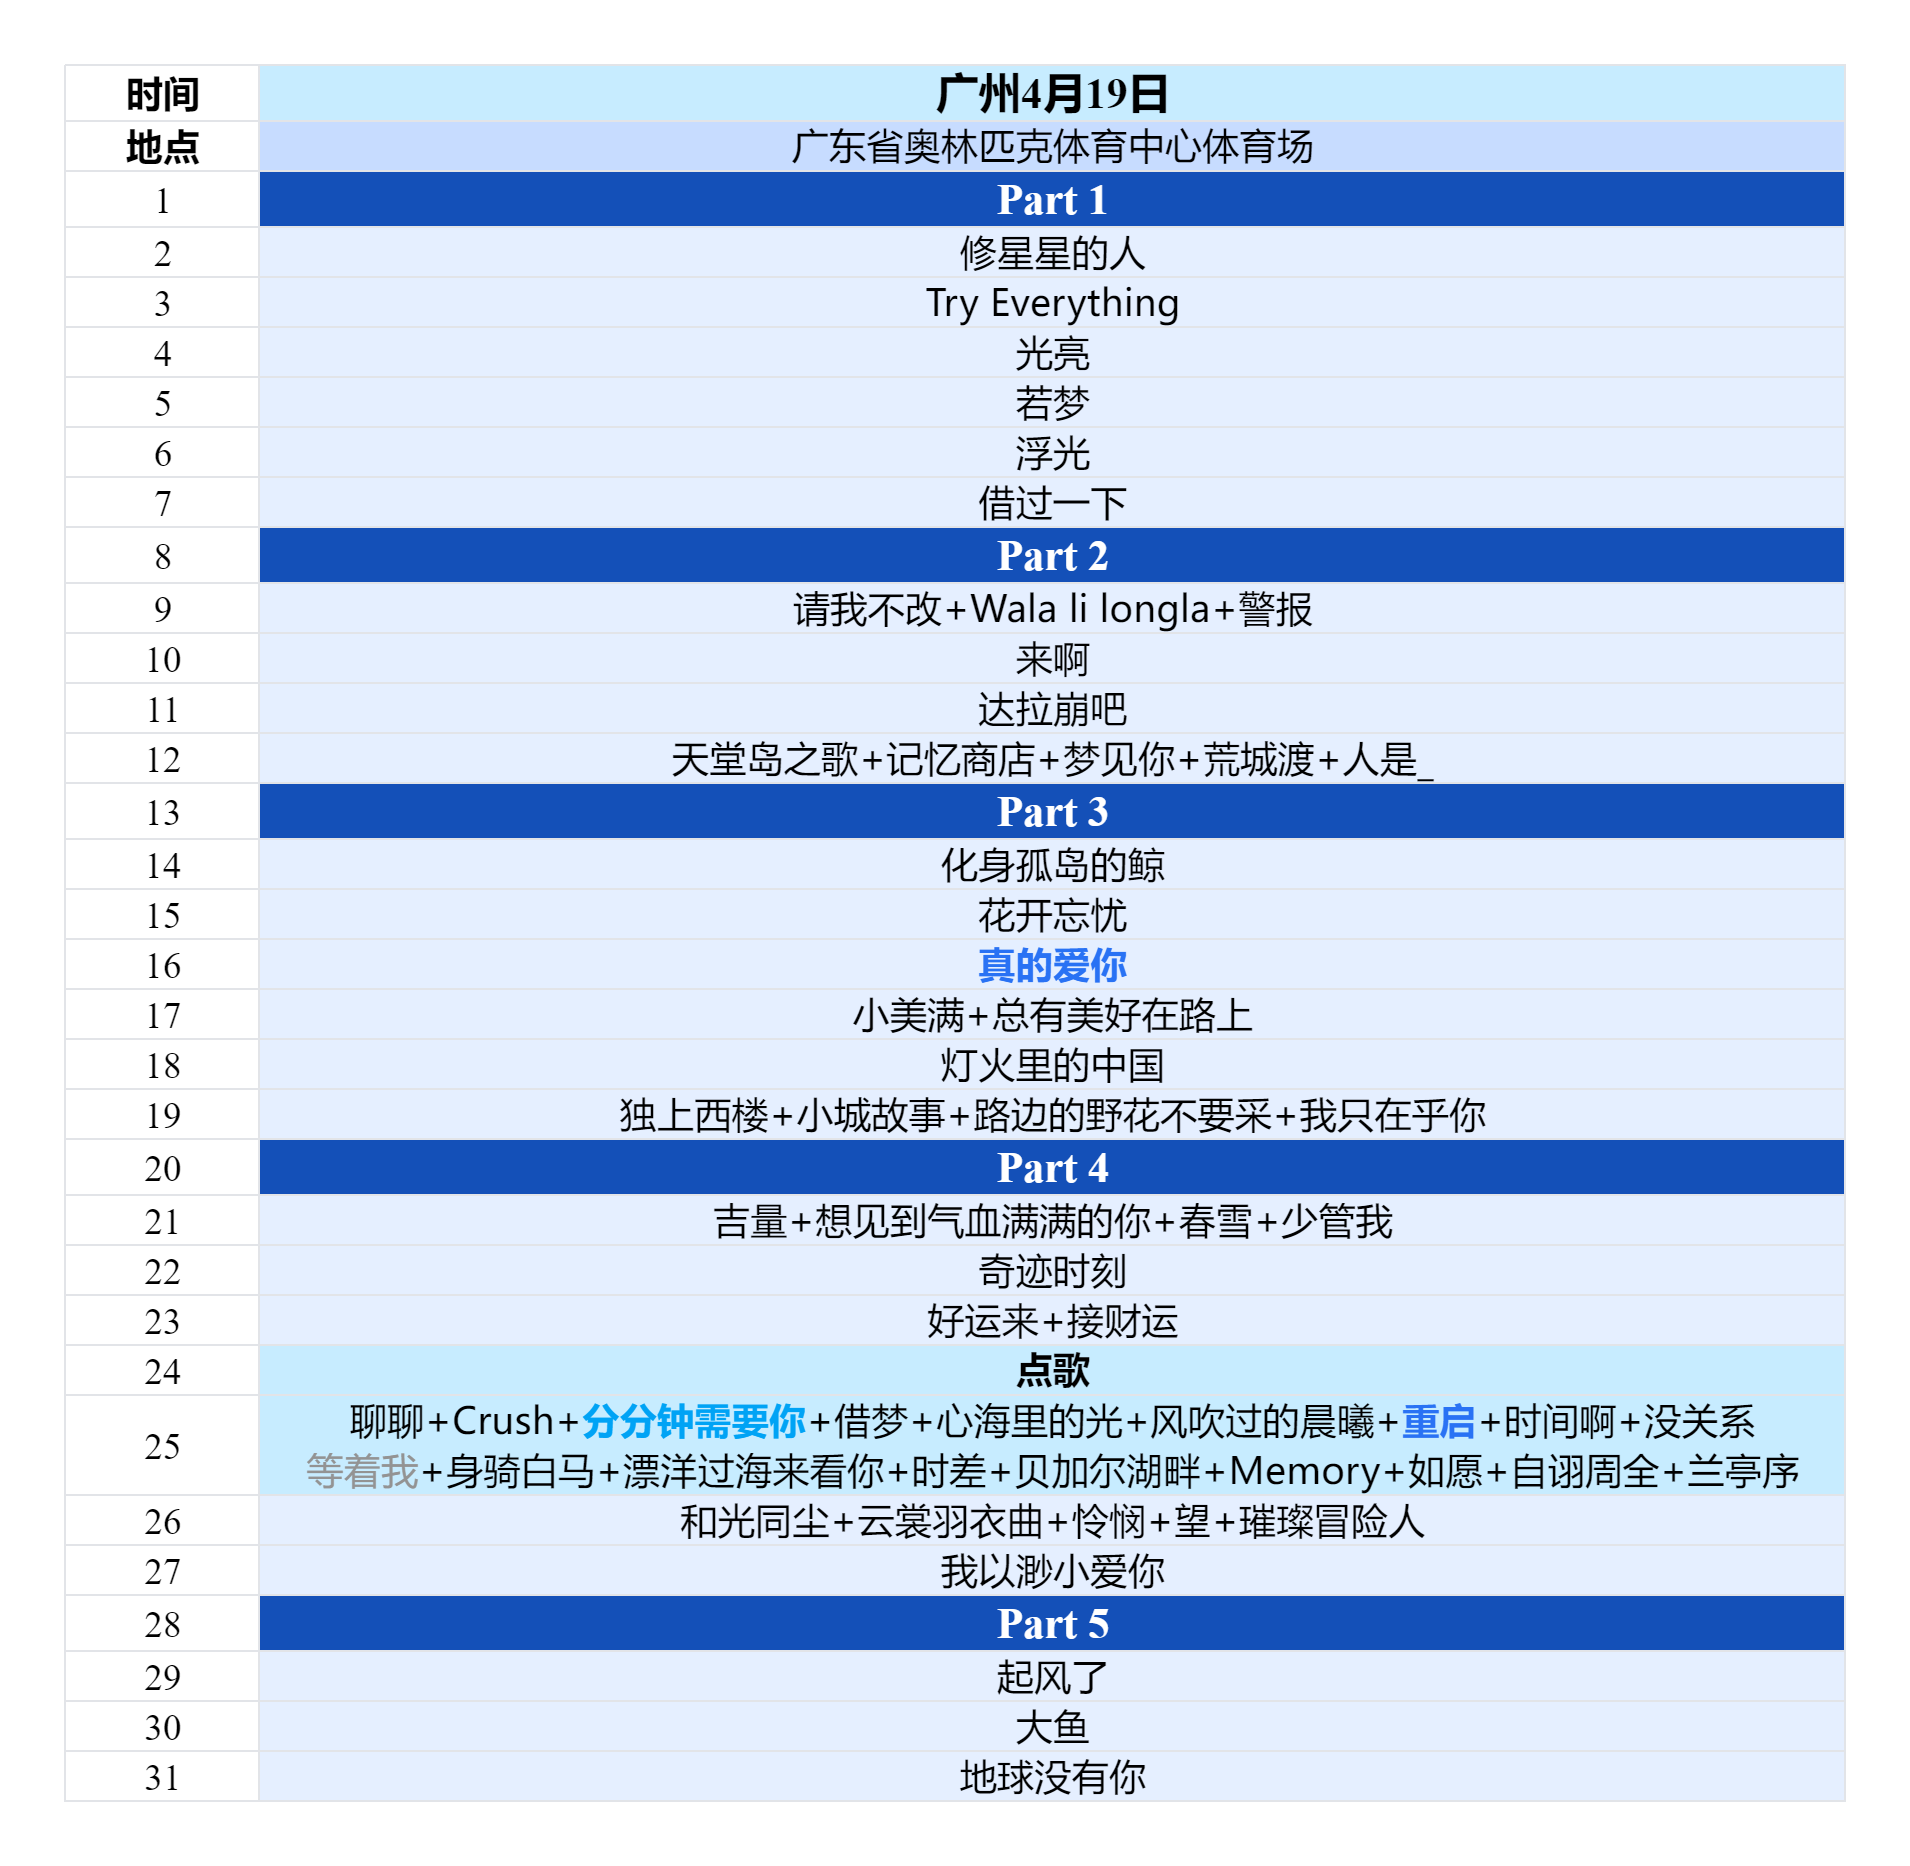
\includegraphics[width=280pt]{img/playlists/GuangZhou-20260419} 

}

\caption{2026周深“深深的”巡回演唱会2026.04.19广州场歌单}\label{fig:unnamed-chunk-7}
\end{figure}

\newpage

\section{Part1}\label{GuangZhou-20260419-part1}

\hyperref[opening-vcr]{🎥【\textbf{开场VCR}】}（VCR 正文见附录 D。VCR 结束后《修星星的人》前奏直接响起，无开场白。）

\hyperref[xiu-xing-xing-de-ren]{🎵【\textbf{修星星的人}】}（VCR 后直接开唱，本首前后无 talking。米：周深！周深！〔前奏中齐喊〕）（深：既然这宇宙让我诞生，想必它是要以我为证）（米：轻声跟唱：既然这宇宙让我诞生）（深：是我在故乡的旷野，仰望银河的夏夜；是我在宇宙的风暴，朝着天仓五飘曳；我的孤独，我的热烈，源自137亿年前\ldots\ldots 在噬星的幻灭里，给太阳撑一把雨伞；在时间的深海里，给地球道一声晚安）（深：我的情感和三十六度的体温，足以暖热即将熄灭的恒星；许我以造物的碎屑，重塑文明的边界；许我以渺小的羞怯，挽留物种的毁灭；在元素的聚散里，给人类抓一把糖果；在星海的倒影里，给生命升一簇篝火）〔已按歌词附录校正〕（深：既然这宇宙予我重生，想必它是要让我看懂，我的基因和闪闪发光的记忆，足以照亮所有星际的永恒）〔高音吟唱收束〕

\hyperref[try-everything]{🎵【\textbf{Try Everything}】}广州的朋友们准备好了吗？（米：欢呼、尖叫）（深：I messed up tonight, I lost another fight, I still mess up but I'll just start again\ldots\ldots Nobody learns without getting it wrong）\ldots\ldots（深、米：Oh oh oh oh\ldots Try everything）〔多轮〕（深：I won't give up, no I won't give in）（米：Till I reach the end and then I'll start again）（深：No I won't leave）（米：I wanna try everything）（深：I wanna try even though I could fail）（深、米：Look how far you've come\ldots\ldots Sometimes we come last but we did our best）〔大合唱〕（深、米：I'll keep on making those new mistakes\ldots\ldots Oh oh oh oh\ldots Try everything）〔多轮收束〕。

  既然这宇宙让我们诞生，我们就不要浪费这一次相遇。你说好不好？（米：好！）你讲，得唔得啊？〔粤语句听写待核〕（米：得！）广州嘅朋友们大家好，大家好，我系周深。你哋好唔好啊？（米：好！）后面的朋友好不好啊？（米：好！）真的好紧张噶。最紧张嘅系，我要在广州的朋友们面前说粤语。但是无论怎么样，我觉得我可能不那么标准的粤语也可以拉近我们彼此的距离，你们说对不对？（米：对！）哇，那是因为你们都太美好了。所以欢迎每一个最可爱的你来到深深的巡回演唱会，你们好吗？（米：好！）我们又一次在深深的相聚了，你们有好好的照顾好自己吗？（米：有！）有没有好好的写自己的人生日记呢？（米：有！）哇，你们看，我去到那么多的地方唱歌，都是因为每一个人把我的人生日记变得这么的精彩。他们换衣服也这么的仓促。〔听写待核〕给我们一点鼓励听听看，有多少人在现场？（米：欢呼、尖叫）呜，好棒。那接下来这首歌，如果你会唱的话，可以跟我们一起唱吗？（米：可以！）因为这所有的美好，所有的奇迹都是因为你身上发出的光才全部的照亮。遇见你，就是我人生当中最美的光亮。（米：欢呼、尖叫）

\hyperref[silver-linings]{🎵【\textbf{光亮}】}（深：海上一阵风吹起，白云涌向陆地，季风带走沙粒，四季冷暖的交替\ldots\ldots 是奔跑中突然袭来的风雨，是黑暗中一根火柴燃烧的光明\ldots\ldots 可是啊我却，愿意去相信，最渺小最微弱最柔软最无畏的你，用尽了全力，努力地去回应，再无边再无尽再无解总有一线生机，光亮你自己）（米：光亮你自己）〔合唱句已按歌词附录校正〕（深：莫听穿林打叶声，一蓑烟雨任平生；竹杖芒鞋轻胜马，谁怕？一蓑烟雨任平生；料峭春风吹酒醒，微冷，山头斜照却相迎；回首向来萧瑟处，归去，也无风雨也无晴）广州的朋友你们好吗？（米：好！）这边的朋友你们好吗？（米：好！）（深：可是啊我却，愿意去相信\ldots\ldots）最无畏的你。（米：欢呼）

  哇，遇见你们，美丽的像一场梦一样。那你们可以把这场梦唱给我听吗？（米：可以！）

\hyperref[like-a-dream]{🎵【\textbf{若梦}】}（深：浮生若梦，为欢几何；风摇雨落，此心何处停泊\ldots\ldots 看天地之间皆漠漠）一个字都不对，太过分了对不对？〔调侃观众接错词〕（米：笑声）（深：往事流转在你眼眸）（米：一边遗忘，一边拼凑）（深：让我听到你！）（深：如我虔诚，合十双手）（米：唯愿你能，得到拯救）（深：情缘若梦，长久几何；一枕含笑，饮下苦涩独酌\ldots\ldots 愿清欢入梦，伴此心停泊）〔已按歌词附录校正〕（米：〔大合唱〕往事流转，在你眼眸）（深：后面的朋友！）（米：〔大合唱〕一边遗忘，一边拼凑，如我虔诚，合十双手，唯愿你能，得到拯救）（深：全场最大声！）（米：〔大合唱〕往事流转，在你眼眸）（深：后面的！）（米：〔大合唱〕一边遗忘，一边拼凑，如我虔诚，合十双手，唯愿你能，得到拯救）因为你\ldots\ldots 哎，今天提前让开了。〔与摄像老师互动〕（米：欢笑、欢呼）你们，我才得到拯救。（米：欢呼、尖叫、口哨声）

\hyperref[floating-light]{🎵【\textbf{浮光}】}人生恍惚三万天，因为遇见了你，才值得留念。你还记得吗？（米：记得------！）（深：弹指间，破晓蝴蝶，煽动一场离别\ldots\ldots 走进熟悉却陌生的思念）你们来唱这里呢。（米：啊\ldots\ldots〔大合唱哼鸣〕）（深：你的眼眸，装满了时间，你的身后，涌动着明天；此生如梦，愿细数流年，与你同写，沧海桑田）到你们！（米：浮光掠影 重山彩云间）全场！（米：你的伏线 穿越千百年）最大声！（米：人生不过 恍惚三万天，漫漫人间 留恋流连）〔合唱句已按歌词附录校正〕。

\hyperref[excuse-me]{🎵【\textbf{借过一下}】}（与上首之间无 talking，直接开唱。深：少年扬起脸庞，前往他的月亮\ldots\ldots 你们都是对的，他说拜托，让开一下）（深：让我大醉一场，殿堂之上，背闲诗两三章；让我穿白衣裳，过疯人巷，去泥潭捞月光）让我听到你的声音好吗？（米：好！）（深唱：让我大醉一场）到你们！（米：殿堂之上）后面的！（米：背闲诗两三章）再来！（深：让我穿白衣裳）（米：过疯人巷）到你们！（合：去泥潭捞月光）（深：望大人们见谅）（米：提点的话）（合：我懂也不想装）再来！（深：世人寻黄金乡）（米：我找月亮）（合：何必偷光）再大声！（合：花谢过 路经过，你是你 我是我）再来！（合：花谢过 路经过，你是你 我是我）哇，很骄傲！（米：噢噢噢噢------〔欢呼〕）你们就是我要寻找的月亮。我找到你们了。（米：欢呼、尖叫）〔借过一下合唱段已按附录 G 校正主干〕

\section{Part2}\label{GuangZhou-20260419-part2}

\hyperref[robot-vcr]{🎥【\textbf{机器人VCR}】}（VCR 正文见附录 D。开篇日期句本场听作''二二二五年五月十七日。今天是我被选中执行任务的第两百天。系统维持正常运转的七万三千天''，与附录 D 一致；VCR 结尾''好的，实验开始''后音乐骤停。）

\hyperref[brave-heart]{🎵【\textbf{请我不改}】}（VCR 结束后电子前奏直接进入。）让我听到你们的声音！（米：噢噢噢噢------！）（深：One, two!）谁在呼唤，耳边徘徊\ldots\ldots〔歌前导句听写待核〕（深：是谁在我耳边念白，说我不配，我不够好，我必失败\ldots\ldots 绝望已经大军压境，回身却没半个人影，才看清追兵与逃兵，竟都是我自己）请我不改，我的姿态！嘿！（米：嘿！）（深：我的爱我的痛都与生俱来；请我不改，我的存在！嘿！）（米：嘿！）（深：我的明我的暗都不必躲开；我原谅我自己，捡起遗憾拥抱无奈；我允许我放手，让我勇敢活在现在；我不等待！嘿！我不徘徊！嘿！）（米：嘿！嘿！）（深：我的笑我的泪都不再苍白，放肆盛开）（米：请我不改！嘿！我的姿态！嘿！我的爱我的痛都与生俱来！请我不改！嘿！我的存在！嘿！我的明我的暗都不必躲开！我原谅我曾怯懦漆黑拥抱无奈。我允许我放手让我勇敢活在现在。我不等待！嘿！我不徘徊！嘿！我的笑我的泪都不再苍白，放肆盛开！）〔全场大合唱整段副歌〕〔已按歌词附录校正〕

\hyperref[wala-li-longla]{🎵【\textbf{Wala li longla}】}（深、米：Wala li longla！Wala li longla！〔全场多轮齐喊〕）（深：Wala\ldots）（米：Wala！）（深：Wala li\ldots）（米：Wala li！）（深：Wala li long\ldots）（米：Wala li long！）（深：Wala li longla！）（米：Wala li longla！）〔逐词递进教学〕（深：全场！）（米：Wala li longla！Wala li longla！〔多轮〕）〔本场 Wala li longla 为《反深代词》``快乐密码''口号互动，穿插在《请我不改》与《警报》之间，含逐词递进教学与全场轮喊多轮〕

\hyperref[jing-bao]{🎵【\textbf{警报}】}（与《请我不改》连唱串烧）警报拉响！（深：我发送警报声，血红色惊叹号，提醒你自救；被遥控，被耗空，快失控，快断送，我替你看透；从借用，到利用，到享用，到滥用，转身就走）\ldots\ldots（深：我学会痛，为你而痛）尖叫声！！（米：全场尖叫）〔本串烧段落已按附录 G 校正主干〕建议把刚才《请我不改》就变成那种有氧的健身操。大家看一下我们舞蹈老师们的汗，就知道。当然也可能是因为广州拥有每一个最可爱的你，所以太热情啦！（米：欢呼、尖叫）后面的朋友你们好吗？（米：好！）那接下来这首歌，跟我一起来好不好？（米：好！）那就来呀！（米：欢呼、尖叫）

\hyperref[lai-a]{🎵【\textbf{来啊}】}（深唱：Don't tell me lie lie lie lie lie）（米：来啊！来啊！来啊！来啊！）（深：我 怎么就感到，感到一不小心就落入圈套\ldots\ldots 将错就错 别拖 Let's go 随你操控 But）一起来！（深、米：Don't tell me lie lie lie lie lie，我望眼欲穿你别闪躲）都叫你------（米：来啊！来啊！来啊！来啊！）（深：有种爱叫痛别退缩）都叫你------（米：来啊！来啊！来啊！来啊！）（深：我倾尽所有，赴汤蹈火）都叫你------（米：来啊！来啊！来啊！来啊！）（深：天赋不只是我，Let's go）我爱你们！（米：欢呼、尖叫）〔来啊合唱段已按附录 G 校正〕

  随机采访，累不累？（米：累！）你今天声音怎么那么浑厚？如果\ldots\ldots 诶，你在广州吃到现在你觉得最好吃的是什么？（观众：我吃的是海鲜。）哦。会不会这个答案有点太平常了一点？说出一个有点特色的。（观众：还是海鲜。生煎。）生煎！同学。好，谢谢你。（米：笑声）好，那接下来到我们深深的巡回演唱会的小游戏啦。我们的荧光棒呢，可以自己选择你喜欢的颜色，分别是蓝色、黄色、粉色和绿色。大家有五秒钟选择颜色的时间。然后呢，不同的颜色代表着不同的角色，无论你选择什么样颜色，你都是人生当中最美的------（米：自己！）系喔，你都系呢个人人生当中最靓嘅仔咯。〔粤语句听写待核〕（米：欢呼、笑声）这一句是不是还可以？（米：可以！）哦，那我的粤语水平真的是时好时坏的。好了，选择完不同的角色之外，就要喊出他们相应的台词。我们试一下啊。达拉崩吧------（米：我最棒！）国王陛下------（米：再说一次！）公主米娅------（米：救我啊！）恶龙------（米：嗷呜！）刚才就当是预习了一遍哈。来，要越来越大声哦。达拉崩吧------（米：我最棒！）国王陛下------（米：再说一次！）公主米娅------（米：救我啊！）恶龙------（米：嗷呜！）公主米娅------（米：救我啊！）公主米娅------（米：救我啊！）达拉崩吧------（米：我最棒！）恶龙乘以十！（米：嗷呜嗷呜！〔重复十次，声音逐渐变大〕）国王陛下乘以五！（米：再说一次！再说一次！再说一次！再说一次！再说一次！）哦，恶龙，刚才是国王陛下让你们再说一次，那恶龙乘以十。（米：嗷呜嗷呜！〔重复十次〕）

  有很多红色的朋友对不对？（米：对！）红色的朋友我们考验一下我们的默契啊，你既然都选择那么倔强的选择了红色，那这个你一定知道。金少刚老师！（米：Polo衫！）不瞒大家说，少刚老师为了我们今年的巡回演唱会非常非常努力，买了十件Polo衫。（米：笑声）十件不同颜色的Polo衫。买到人家商家都说，相同的款式真的要印这么多颜色吗？（米：笑声）金少刚老师！（米：Polo衫！）安栋老师！（米：小西装！）也不瞒着大家说，广州都这个天气了，还在穿小西装。（米：笑声、欢呼）人设会不会有点太稳定了？我的爪子穿成这样合理吗？〔听写待核〕（米：笑声、欢呼）那接下来这首歌，跟我一起来，达拉崩吧！（米：欢呼、尖叫）来，声音不够大，达拉崩吧！

\hyperref[dalabengba]{🎵【\textbf{达拉崩吧}】}（深：很久很久以前，巨龙突然出现，带来灾难，带走了公主又消失不见\ldots\ldots 他说，陛下我叫，达拉崩吧斑得贝迪卜多比鲁翁）是不是，达拉崩吧斑得贝迪卜多比鲁翁？（米：达拉崩吧斑得贝迪卜多比鲁翁！）对对，达拉崩吧斑得贝迪卜多比鲁翁！（米：达拉崩吧斑得贝迪卜多比鲁翁！）达拉崩吧！（米：我最棒！）国王陛下！（米：再说一次！）公主米娅！（米：救我啊！）恶龙！（米：嗷呜嗷呜！）（深：英雄达拉崩吧，骑上最快的马，带着大家的希望，从城堡里出发\ldots\ldots 闯入一座山洞，公主和可怕的巨龙，英雄拔出宝剑，巨龙说，我是昆图库塔卡提考特苏瓦西拉松）再来一次，昆图库塔卡提考特苏瓦西拉松！（米：昆图库塔卡提考特苏瓦西拉松）是不是，昆特牌提琴烤蛋挞苏打马拉松？（米：笑声）不对！是，昆图库塔卡提考特苏瓦西拉松！（米：昆图库塔卡提考特苏瓦西拉松）达拉崩吧！（米：我最棒！）国王陛下！（米：再说一次！）公主米娅！（米：救我啊！）恶龙！（米：嗷呜嗷呜！）（深：于是，达拉崩吧斑得贝迪卜多比鲁翁，砍向，昆图库塔卡提考特苏瓦西拉松；救出了，公主米娅莫拉苏娜丹妮谢莉红，回到了，蒙达鲁克硫斯伯古比奇巴勒城\ldots\ldots 从此他们幸福地生活在一起）达拉崩吧！（米：我最棒！）国王陛下！（米：再说一次！）公主米娅！（米：救我啊！）恶龙！（米：嗷呜嗷呜！）金少刚老师！（米：Polo衫！）安栋老师！（米：小西装！）全名，他们叫------（米：达拉崩吧斑得贝迪卜多比鲁翁！）这么爱念，要念你来念吧！（米：欢呼、尖叫、大笑）哇，达拉崩吧，随着你们唱的声音越来越大声，越来越好听。你们知道自己唱得很好听吗？（米：知道！）（米：笑声）这怎么会有这么多人好意思这样说？``知道''！你唱得这么好听，那你上来唱咯。你们是来踢馆的是吗？（米：笑声）大家记得我前年有一张专辑叫做------（米：反深代词！）《反深代词》里面有一栋蜃楼。在我们去年的小穿梭当中，被困在了蜃楼当中出不来，对不对？（米：对！）那，它后面发生了什么事情呢？让我们来看看吧。（米：欢呼、尖叫）

\hyperref[haven-song]{🎵【\textbf{天堂岛之歌}】}（VCR配音：救我！这是哪里？）（米：你心里！〔全场笑〕）（深：叮咚，我有一个秘密，悄悄告诉你，欢迎你来到天堂入口；叮咚，有人在按门铃，是谁在外面，把恶作剧当一场游戏；听啊，谁在哭泣，看啊，谁在窃窃私语，窗外有双眼睛，它在时刻注视着你；叮咚，有人在看你的过去，叮咚，有人在看你的现在\ldots\ldots 我逃不出去，我逃不出去，我逃不出去）〔已按歌词附录校正〕。

\hyperref[the-memory-store]{🎵【\textbf{记忆商店}】}（深：有客人从夜里来，买很古老的年代\ldots\ldots〔短暂演唱后转说白，歌词听写待核〕）哦，我知道了，这里是《反深代词》当中的记忆商店。那我们在广州一定创造了非常非常美好的记忆，对不对？（米：对！）传说只要拥有这一颗米子心，也就是米子和周星星。〔听写待核〕（米：欢呼、尖叫）大家就可以在记忆商店购买你最想念的那一颗记忆哦。（米：欢呼、尖叫）

\hyperref[meng-jian-ni]{🎵【\textbf{梦见你}】}（深：看着眼前，还年少的你，恍如流年从未淌过去\ldots\ldots 离别是相遇的倒影，从初问候的那天起，就有了再见的回音\ldots\ldots 但愿那时你在人海里，仍将我一眼认清）〔已按歌词附录校正〕（合：无数个没有你的季节\ldots\ldots〔观众合唱句，两轮听写不一致，听写待核〕）想念的人一定会再见的，对不对？（米：对！）

\hyperref[huang-cheng-du]{🎵【\textbf{荒城渡}】}（深：夜色中寻觅过，当往事困住我，也盼心中生出一点萤火\ldots\ldots 断了这心魔，可原谅我，宿命中获得这解脱，重来过）（深：眼中浮沉，手中残魂，那故事斑驳荒城\ldots\ldots 想念天真，拨开心门，我宁可踏破这孤身）〔合唱句已按歌词附录校正〕（合：无数个没有你的季节\ldots\ldots〔观众合唱句，听写待核〕）（深：啊\ldots\ldots〔高音吟唱〕）（米：欢呼、尖叫）

\hyperref[Humans_are_]{🎵【\textbf{人是\_}】}（深：未知摊开棋局，舍弃昨日才可破，再见了我的月光，我的蓝，我的爱\ldots\ldots 让死亡觊觎我，让恐惧亲吻我，来摧毁我深爱的一切，可仍夺不走我的选择）你们帮我！（米：让死亡觊觎我，让恐惧亲吻我，来摧毁我深爱的一切，可仍夺不走我的选择）（深：弹指间湮灭我）（米：但命运打不败活着）（深：让生命如剧烈的烟火，璀璨熄灭前也将点亮，孩童的双眸，未来的瞳孔）（米：让死亡觊觎我，让恐惧亲吻我\ldots\ldots 我们依然前行，没有光指引）〔大合唱段落〕（深：不朽的，永恒的，都被你们记住了吗？对不对？）（米：欢呼、尖叫）〔已按歌词附录校正〕

\section{Part3}\label{GuangZhou-20260419-part3}

\hyperref[music-animations-vcr]{🎥【\textbf{音乐动画VCR}】}（VCR 正文见附录 D。本场动画结尾有一句旁白------``回忆虽然美好，但是因为有了你，我们更要继续往前行，对不对？''〔听写待核，与 0418 场所听''如果遇到了你，我们一定可以好好享受现在。挣脱才能定义的束缚''不同，建议对照官方视频〕）（米：对！〔欢呼、尖叫〕）〔VCR 后为纯音乐过场〕

\hyperref[The-whale-who-became-an-island]{🎵【\textbf{化身孤岛的鲸}】}（深：La la la\ldots\ldots〔吟唱引入，前奏中〕）广州第二场的朋友们你们好吗？（米：好------！）可以让我听到你的声音吗？（米：可以------！〔欢呼、尖叫〕）（深：我是只化身孤岛的蓝鲸，有着最巨大的身影，鱼虾在身侧穿行，也有飞鸟在背上停\ldots\ldots 我爱地中海的天晴，爱西伯利亚的雪景，爱万丈高空的鹰，爱肚皮下的藻荇，我在尽心尽力地多情，直到那一天）到你们了！（米：我是只化身孤岛的蓝鲸，有着最巨大的身影，鱼虾在身侧穿行，也有飞鸟在背上停〔大合唱〕）再大声！（米：我有着太冷太清的天性，对天上的她动过情，而云朵太远太轻，辗转之后各安天命）最大声！（米：我未入过繁华之境，未听过喧嚣的声音，未见过太多生灵，未有过滚烫心情，所以也未觉大洋正中，有多么安静）再来！（米：你的衣衫破旧，而歌声却温柔，陪我漫无目的的四处漂流）（深：我的背脊如荒丘，而你却微笑摆首，把它当成整个宇宙）（米：你与太阳挥手，也同海鸥问候，陪我爱天爱地的四处风流）（深：你的指尖轻柔，抚摸过我所有，风浪冲撞出的丑陋疮口；你眼中有春与秋，胜过我见过爱过的一切山川与河流；曾以为我肩头是那么的宽厚，足够撑起海底那座琼楼，而在你到来之后，它显得如此清瘦，我想给你能奔跑的岸头）（米：欢呼、周深！周深！）

  （深：你们有多少个墙头？）（米：没有！）科普一下，墙头的意思就是说，每当你问他们，``你喜欢哪个歌手啊？''（米：周深！）他们会这样回答，然后会问，``你们只喜欢周深吗？''（米：是！）那通常情况下是在说谎骗人。（米：没有！）他们还会喜欢很多其他歌手。（米：没有！）我居然好意思说人家叫其他的歌手了，他们就叫墙头。但是无论如何，你们都是我的国王和王后。（米：欢呼、尖叫）

\hyperref[Blossoms-that-forget-sorrow]{🎵【\textbf{花开忘忧}】}我们来广州看你咯。（米：欢呼）有没有好好照顾好自己呀？（米：有！）一定要做到好吗？（米：好！）（深：巷子口买了花，穿过沿街红墙青瓦\ldots\ldots 一件遗憾的事就喝一碗汤，庭院深深，秋叶飘落）（深：我们苍老的时候就回到小时候，采青梅用来酿酒你不许偷着喝，穿朴素的衣裳牵着那衣袖，捡了小猫名为苍狗）我说，说什么？（米：你好啊！）你们好吗？（米：好！）（深：这是给你的花，花的名字叫忘忧草，它说时光汹涌如水上烟波，别走远了一起回家）我们来广州看你咯！（米：欢呼）（深、米：我们苍老的时候就回到小时候\ldots\ldots 在梦里做个梦，看见你我都老了；那永恒没骗我，离散也没有；这份爱只是活在另外时空；如果每一声再见会开启一个新的空间，每做一个梦是时空偶尔的重叠；你好吗，离开的人啊，请帮我相爱到剧终）（深：忘忧草开着花，你在月光下不说话，一件遗憾的事就喝一杯茶，庭院深深，秋叶飘落）〔合唱句已按歌词附录校正〕（米：妈妈不哭！〔有观众感动喊出〕）（米：欢呼、尖叫）

  我们的人生当中一定有那一个非常非常重要的人，他的力量一直在陪着你，鼓舞着你。但是呢，也有那一份遗憾。就像我的老师，他都没有办法看到我被那么多人听到。所以谢谢你们，让我被听到了，谢谢你们！（米：欢呼、尖叫、谢谢周深！）所以一定要好好的照顾好自己。因为我们思念的人，他一定听得见，对不对？（米：对！）花开忘忧，愿你无忧。花开忘忧\ldots\ldots（米：愿你无忧！）谢谢。我呢，就开始说我的粤语。虽\ldots\ldots 我说的不标准你们不会怪我哈？（米：不会！）虽然呢我这个\ldots\ldots 我我嘅广东话咧真的唔得，但系咧我真的好中意听广东话嘅歌啦。（米：欢呼、尖叫）昨天那首大家唱的特别好听，我想听你们再唱一下。（深、米：苦海翻起爱恨，在世间难逃避命运，相亲竟不可接近\ldots\ldots）〔昨日场《一生所爱》副歌再现〕（米：笑声）我听出来是不记词了哈。那今天这首我也非常喜欢，叫做《真的爱你》。（米：欢呼、尖叫）你们会唱吗？（米：会！）我也是真的爱你们哟。（米：欢呼、尖叫）也要好好的爱我们的妈妈好不好？（米：好！）也同样要好好爱一直默默爱着我们的人好不好？（米：好！）如果你内向，害怕说出来，那就用最大的声音唱出来好不好？（米：好！）让我听到你的声音，你们好吗？（米：好！）

\hyperref[zhen-de-ai-ni]{🎵【\textbf{真的爱你}】}（深、米：无法可修饰的一对手，带出温暖永远在背后，纵使啰嗦始终关注，不懂珍惜太内疚；沉醉于音阶她不赞赏，母亲的爱却永未退让，决心冲开心中挣扎，亲恩终可报答；春风化雨暖透我的心，一生眷顾无言地送赠）全场！（米：是你多么温馨的目光，教我坚毅望着前路，叮嘱我跌倒不应放弃；没法解释怎可报尽亲恩，爱意宽大是无限，请准我说声真的爱你）我系真的爱你啊！（米：欢呼、尖叫）（深、米：无法可修饰的一对手\ldots\ldots 仍记起温馨的一对手，始终给我照顾未变样，理想今天终于等到，分享光辉盼做到；春风化雨暖透我的心，一生眷顾无言地送赠）全场！（米：是你多么温馨的目光，教我坚毅望着前路，叮嘱我跌倒不应放弃）再大声！（米：没法解释怎可报尽亲恩，爱意宽大是无限，请准我说声真的爱你）我系真的好爱你呀！（米：欢呼、尖叫）要好好的爱我们爱的人，一直默默爱着我们的人好不好？（米：好！）尖叫声在哪里？（米：欢呼、尖叫）我要听到你们最大声的合唱！（米：是你多么温馨的目光\ldots\ldots）大声！（米：教我坚毅望着前路，叮嘱我跌倒不应放弃）谢谢每一个听到我的人！（米：欢呼）哇！太好听了！我想单独再听一下好不好？（深领唱：是你多么温馨的目光）（米合唱：教我坚毅望着前路）（深领唱：叮嘱我）（米合唱：跌倒不应放弃）（合：没法解释怎可报尽亲恩，爱意宽大是无限，请准我说声真的爱你）（深独唱：请准我说声）（米大合唱：真的爱你！）（米：欢呼、尖叫）要好好的爱一直默默爱着我们的人好吗？（米：好！）〔唱词已按歌词附录校正〕

\hyperref[simple-bliss]{🎵【\textbf{小美满}】}那这首歌你们会唱吗？（米：会！）那也会大声跟我一起唱吗？（米：会！）（深、米：没什么大愿望，没有什么事要赶；看见路口红灯一直闪，它像眨眼的小太阳；乌云还挺大胆，顶在头上吹不散，我抓在手里捏成棉花糖，什么烦恼不能忘；既然是路一定有转弯，哪个风景都漂亮，揉揉疲惫的眼睛停下来看一看，美好简单）全场最大声！（深、米：你看小狗在叫，树叶会笑，风声在呢喃；不如好好欣赏一秒迷迷糊糊的浪漫；只要一觉醒来床单洒满阳光的温暖，不去想不必想不用急急忙忙说一个答案）答案就是被你们听到了很幸福！（米：欢呼、尖叫）准备好了吗？（深、米：笑一笑就灿烂，唱一句歌就舒展，收集一点一滴小美满，都是幸福的花样，没道理的开朗；打扮平凡的日常，找到自己最合身的衣裳，只要自己够喜欢，至少还有温柔的眼光，还在夜里看月亮，心情铺得再满也要留一扇天窗，岁月很长）亲爱的朋友们，谢谢你们送我这么多特别特别美丽的小美满，谢谢你！（米：谢谢周深！）来让我们一起在深深的巡回演唱会许愿好不好？（米：好！）后面是一棵许愿树。就像我这样闭上眼睛，想好愿望，然后我倒数三、二、一，睁开眼睛，我们的愿望就会出现在许愿树上哦。现在现场的每一个朋友，无论什么年龄段，无论什么职业，闭上眼睛，许个愿吧。想想生日的时候一直想要许什么愿呢？想想一直想要做的什么事情呢？哦对了，在小美满当中的愿望，只能够许关于自己的愿望。想一想，是不是很久或者是从来没有跟自己说过，你真的很棒。你辛苦啦。你走到现在真的非常非常了不起哦。你真的很优秀。想一想是不是从来没有拥抱过自己啊？三、二、一，睁开眼睛！（米：欢呼、尖叫）（深：笑就好，哭也好，今天就是明天最好的陪伴）到你们唱！（米：自己就是自己最好的陪伴）（深：靠你们了！）（米大合唱：自己就是自己最好的陪伴！）（深：你们的出现，就是周深最好的陪伴。）（米：欢呼、尖叫）

\hyperref[zong-you-mei-hao-zai-lu-shang]{🎵【\textbf{总有美好在路上}】}（深、米：花在开，云在飘，笑容在脸上，我们向前方一路向阳）到你们！（米：亲爱的你，在路上慢慢逛，看一看太阳；让风轻轻，吹拂你的脸庞）（深、米：今天过去，要到明天看看天气会怎样，阴或晴朗，故事都慢慢赏；抬头发现，你就是光芒）〔本场收句现场改词''你就是光芒''，录音室版作''光一直在身上''〕因为你们就是光啊！（米：欢呼、尖叫）

\hyperref[deng-huo-li-de-zhong-guo]{🎵【\textbf{灯火里的中国}】}灯火里的中国，之所以这么美丽，是因为有每一个最可爱、一直在发着光的你。等一下跟我一起唱好吗？（米：好！）（深：都市的街巷已灯影婆娑，社区暖暖流淌的欢乐，远山的村落火苗闪烁，渐渐明亮小康的思索\ldots\ldots 归港的船帆从灯塔掠过，追梦脚步月下交错，广场焰火在节日诉说，星空升腾时代的巍峨）等下让我听到你们最大声好不好？（米：好！）谢谢你们。全场唱！（米：灯火里的中国，青春婀娜；灯火里的中国，胸怀辽阔；灯火灿烂的中国梦，灯火荡漾着心中的歌）（深：再来！）（米：灯火里的中国，青春婀娜；灯火里的中国，胸怀辽阔；灯火灿烂的中国梦，灯火荡漾着心中的歌）（深：再唱！）（米：灯火荡漾着心中的歌）（深：心中的\ldots\ldots 的歌\ldots\ldots〔高音收束，哼鸣收尾〕）（米：欢呼）。

  接下来，又到了我介绍我担的时候啦。希望我好好唱歌，让以后你们出去介绍你们担的时候也那么有底气。（米：欢呼）我担的名字叫做------（米：邓丽君！）礼貌点，邓丽君女士。（米：笑声）对，我担的名字叫做------（米：邓丽君女士！）哦，好听话哦。（米：笑声）那我相信她有很多很多歌，你们一定听过。哦，小朋友应该也听过哦，等下可以试一下啊。好，那我们来听一下这些歌当中有没有你喜欢的歌喽。那等下一定要跟我最大声音唱好不好？（米：好！）

🎵【\textbf{邓丽君组曲}】

\hyperref[du-shang-xi-lou]{🎵【\textbf{独上西楼}】}（深：无言独上西楼，月如钩，寂寞梧桐，深院锁清秋；剪不断，理还乱，是离愁，别是一般滋味在心头；这一刻，心的歌声，又是你的墙头〔现挂，听写待核〕）（米：没有！〔全场大喊〕）来到广州，跟你们相遇是最美的故事。跟我一起唱！

\hyperref[xiao-cheng-gu-shi]{🎵【\textbf{小城故事}】}（深：广州故事多〔现场改编''小城故事多''〕）来！后面的朋友大声点！（米：充满喜和乐）（深：若是你到广州来〔现场改编〕）（米：收获特别多）（深：看似一幅画）（米：听像一首歌）（深：人生境界真善美）（米：这里已包括）（深、米：谈的谈，说的说）（深：看看谁的墙头多！）（米：没有！）（深、米：请你的朋友一起来）（米：广州来做客〔现场改编''小城来做客''〕）来哪里？（米：广州来做客！）厉害！大声唱好不好？（米：好！）

\hyperref[donot-pick-the-roadside-flowers]{🎵【\textbf{路边的野花不要采}】}（深、米：送你送到小村外，有句话儿要交代；虽然已经是百花开）（深：墙头多的人听到喽！〔现场改词调侃〕）（深、米：路边的野花，你不要采）（深：全场！）（深、米：记着我的情，记着我的爱，记着有我天天在等待；我在等着你回来，千万不要把我来忘怀，千万不要把我来忘怀，千万不要把我来忘怀）什么？（米：我忘怀！〔笑声〕）你们会忘了我吗？（米：不会！）谢谢你们出现在我的人生当中。（米：谢谢周深！）

\hyperref[I-only-care-about-you]{🎵【\textbf{我只在乎你}】}（深、米：如果没有遇见你，我将会是在哪里；日子过得怎么样，人生是否要珍惜；也许认识某一人，过着平凡的日子，不知道会不会也有爱情甜如蜜）（深：大声唱！）（深、米：任时光匆匆流去，我只在乎你；心甘情愿感染你的气息）（深：最美合唱团！）（深、米：人生几何能够得到知己，失去生命的力量也不可惜，所以我求求你，别让我离开你，除了你我不能感到一丝丝情意）（深：再大声！）（深、米：任时光匆匆流去，我只在乎你；心甘情愿感染你的气息）（深：大声唱！）（深、米：人生几何能够得到知己\ldots\ldots 除了你我不能感到一丝丝情意）（深：全场！）（深、米：除了你，我不能感到一丝丝情意）（深：我不能感到一丝丝情意。不能没有你！〔收束句听写待核〕）（米：欢呼、尖叫）

\section{Part4}\label{GuangZhou-20260419-part4}

\hyperref[mask-vcr]{🎥【\textbf{面具VCR}】}（VCR 正文见附录 D。开篇日期行本场为''2026年4月19日，广州''，其余与附录 D 一致，含''我就戴上了一个幺蛾子面具，还有一个背包客面具''〔蒙面唱将猜猜猜面具梗〕。）

（米：对！！！）〔回应 VCR 结尾''你说，对吗？``〕你们听到了吗？（米：听到了！）好吗？（米：好！）（米：欢呼、尖叫）

\hyperref[ji-liang]{🎵【\textbf{吉量}】}（深：羲和车上金铃铛）（米：叮当，叮当）（深：望舒驾后银尾巴，摇摇晃晃）（深：弱水岸边唤吉量，吉量吉量）（米：叮叮当当，叮叮当当）（深：九天之上飘来一朵雪花，原来是我的英俊的小马，金色星星在它眼里安家，祝融手持火种编织了它的发）〔已按歌词附录校正〕你们声音有多大？（米：大！）（深：我的小马一天一天长大，穿过凛冬和最沸腾的夏，衔来西边石头东边的花，马蹄扬起层层层层的云纱）会唱的一起！（米：〔合唱〕）（深：高高山上鸾鸟唱，叮当叮当；东海浪里搅银汤，汤汤荡荡；建木树下唤吉量，吉量吉量；叮叮当当，天地叮叮当当）〔已按歌词附录校正〕（深：吉量，我勇敢的小马，当人间需要桥梁，请你垂下缰；吉量，树顶上那颗太阳，在晨雾里张望，驮它来我身旁）谢谢你们的出现！（米：欢呼、尖叫）迎光吧！〔听写待核，疑为''荧光棒''〕（米：欢呼、尖叫）

  （深：你是谁？你是自己的宝贝！）（米：宝贝！）〔接唱入曲〕

\hyperref[xiang-jian-dao-qi-xue-man-man-de-ni]{🎵【\textbf{想见到气血满满的你}】}（接上首连唱）（深：有时候感觉自己多珍贵，还会有更好的等着你，还有好多梦在飞，还要给自己一个新的机会；要早起早睡，别那么累，做好气血满满的准备）你们好吗？（米：好！）（深：再疼再冷再怕的时候，请你一定记得，我永远会是你停靠的选择。）哈喽？（米：我永远是你最好的选择！〔观众抢答〕）（深：我有梦可追，勇气可归，举起热情满满的奖杯，那时的你，灿烂的你，无惧也无畏；无论多少岁，精神百倍，我都会来陪着你找回，春天又来，生命又来，阳光的明媚）要时刻记得，你是自己的------（米：宝贝！）而且，你们也都是我的宝贝哦！（米：欢呼、尖叫）要好好照顾好自己好吗？（米：好！）就像第一首歌唱的一样，既然宇宙让我们诞生了，我们就一定要好好的享受每一次相遇对不对？（米：对！）加油！让小火车以及我们的步伐继续向前出发吧！（米：欢呼、尖叫）你好！谢谢你们来看我哦！

\hyperref[chun-xue]{🎵【\textbf{春雪}】}（深：白是梦境的泥土，白是回忆的发束，有些记忆依然自反复，练就成我们的天赋，也不免在这一生寒苦；冰是血色的礼物，却努力重来时的温度，融化难以碰触，沿着心底泛流关注，让面孔化作纪念）注意安全！〔已按歌词附录校正〕你们好！（米：好！）（深：我想在冬夜雪地与你追逐，你却落在早春中的一棵树；一次错过不算错误，错在来不及，看清楚你的面目我就交出全部）到你们！（米：我想在冬夜雪地与你追逐）你们好漂亮好帅气呀！（米：欢呼、尖叫）（深、米：雪花开在冬夜深处蔓延，蔓延到一个危险的春天；春天蚕食消融目空一切，一切啊那曾是我的世界；我在原地守护我的体面，春天再见，春天再见；我还在冬夜雪地里等日出，你落满早春枝叶宣判我输；趁着交迫还没结束，在这一条必经之路，我下慢了脚步，陪你庆祝）〔已按歌词附录校正〕

  在做自己的路上，如果遇到一些杂音，在不打扰别人的前提下，说一声''嘿''！（米：嘿！少管我！）

\hyperref[watch-ur-manners]{🎵【\textbf{少管我}】}嘿！少管我！（米：欢呼、尖叫）（深：无数麻烦是想要无聊的理由，把沉重身体传送到热带气候，脑袋放空，吹吹海风，用一场远行当做逃离的方舟；做生活困兽不如去浪漫宇宙）你们好！（米：好！）（深、米：我想我可以，抓住风中飘散的花，不介意坠入水星或是泥巴，跟现在握手拥抱道别出发，别停下）（深、米：我想我成为阳光蔷薇飞鸟盛夏，或成为昆虫砂砾一片雪花）三二一！嘿！（米：嘿！少管我！）五四三二一！嘿！（米：嘿！少管我！）再来！嘿！（米：嘿！少管我！）呜------！五四三二一！嘿！（米：嘿！少管我！）我爱你们！（米：欢呼、尖叫）（深、米：我想我可以，抓住风中飘散的花\ldots\ldots 我想我成为阳光蔷薇飞鸟盛夏，或成为昆虫砂砾一片雪花）Hello!（深、米：让这趟旅途，开始书写新的束缚，对明天毫无保留）三二一！嘿！（米：嘿！少管我！）五四三二一！嘿！（米：嘿！少管我！）哇，我刚才有看清好多好多朋友们的脸哦。你们真的好帅气、好美丽、好温暖、好治愈。谢谢你们出现在这个世界上。谢谢你们！（米：欢呼、尖叫）因为啊，被你们看见是非常非常幸福的一件事情。所以要好好照顾好自己好吗？（米：好！）《少管我》这首歌就像刚才那样一样，是轻松欢快的歌，不是让我们去争执。所以呢，在寻找自己的路上，如果遇到一些杂音，在不打扰别人的前提下，我们轻松地说一句：嘿！（米：嘿！少管我！）被你们听见，被你们看见，怎么能够说它不是奇迹时刻呢？（米：欢呼、尖叫）

\hyperref[miracle-moment]{🎵【\textbf{奇迹时刻}】}（深：藏进发光的恒星，穿梭时空的王牌，每个瞬息都能将苦涩一键更改\ldots\ldots I wanna see my way in the starlight，奇迹时刻等你一起来，开启夺目现在；We gonna change the fate never deny，以无数个渺小的光彩，就能照亮无穷未来）〔已按歌词附录校正〕加油！（米：欢呼）这是昨天坏了的那个吗？〔调侃昨日场魔术道具〕（米：笑声）全场！（深、米：这世界总有太多无力更改，引起是非，引起期待；我相信谁都可以重塑现在，不需要等待，Show Time，此刻就无限精彩）〔已按歌词附录校正〕

  魔术时间到！掌声在哪里？（米：欢呼、尖叫）我的魔术，也许带不来大为震撼，但是可以让你们为我捏一把汗。（米：笑声）这是一支笔对不对？（米：对！）没有问题哦。没有问题哦。但是你们看！如果我把它\ldots\ldots 穿过这个小小盒子\ldots\ldots 它就可以消失一块！（米：惊呼：哇------！）你们看还可以动哦。（米：惊叹声）当当！（米：欢呼、尖叫）给我倒数三个数可以复原它。三、二、一！（米：三！二！一！〔欢呼〕）还有！你们看！这里有个红球对不对？它现在是在比较矮的一边对不对？我可以用魔法把它变到高的那一边里面去，你们相不相信？（米：相信！）来喽！我需要倒数五个数字！（米：五！四！三！二！一！）〔欢呼、尖叫〕我跟你们说，今天两个魔术都成功。（米：欢呼）那些想看我魔术出丑的人，没想到吧？其实这个魔术刚才差点失败。但是我做到了！那请问，好运来了，你们接不接？（米：接！！！）广州的朋友们，接好运咯！（米：欢呼）后面的朋友大声唱哦！

\hyperref[good-fortune-comes]{🎵【\textbf{好运来}】}（深、米：好运来祝你好运来，好运带来了喜和爱，好运来我们好运来，迎着好运兴旺发达通四海）（深：叠个千纸鹤，再系个红飘带，愿善良的人们天天好运来\ldots\ldots 你凤舞太平年，你龙腾新时代，你幸福的家园迎来百花盛开）全场！（米：好运来祝你好运来，好运带来了喜和爱，好运来我们好运来，迎着好运兴旺发达通四海）大声唱！（米：好运来祝你好运来\ldots\ldots〔多轮〕）祝大家每天好运，大家接不接？（米：接！）新的一天，我们所有的幸福，所有的美好，我们都用最大的声音把它接到自己身边好不好？（米：好！）

\hyperref[jie-cai-yun]{🎵【\textbf{接财运}】}一起接平安！（米：接平安！）一起接幸福！（米：接幸福！）一起接健康！（米：接健康！）一起接财运！（米：接财运！）（深、米：接个好运来，接个福气来，接个财神开开心心到我家里来；接了才应验，潇洒又自在，我接，我接，我接金山银海）〔已按歌词附录校正〕（米：好运来，我接个好运来，我接个福气来，我接个大舞台〔合唱句听写待核〕）祝所有朋友，恭喜发财！好运来！（米：欢呼、尖叫）接不接？（米：接！）哇，不够大声，接不接？（米：接！）爱你们啊！（米：欢呼、尖叫）

【\textbf{点歌环节}】
  接下来，要接的是我们的点歌环节。（米：欢呼、尖叫）好礼貌性的''呜''。仿佛也不是很期待的''呜''。也总要点点歌嘛对不对？呜------（米：欢呼、尖叫）力挽狂澜。大湾区真的很棒。哎，昨天他们唱有首歌很好听，你们会唱吗？（米：会！）（深唱：一滴水）（米：一滴水\ldots\ldots〔合唱接唱〕）（深唱：是咸的，那是感动的眼泪）（米：是咸的，那是感动的眼泪〔合唱接唱〕）（深：Hello？）（深唱：一汪水）（米：一汪水\ldots\ldots〔合唱接唱〕）（深唱：太深太深太深也看不清）（米：太深太深太深也看不清〔合唱接唱〕）（深唱：清澈的\ldots\ldots）哎，你们怎么不接这句啊？我只记得后面那一句。〔昨日场全运会开幕式''一滴水''梗再现，歌名待核〕来喽，全场帮我倒数五个数字。五、四、三、二、一，停！（米：欢呼、尖叫）您好。（观众：你好。嗨宝贝。）（米：欢呼、尖叫）宝你个头啊。请问怎么称呼您？（观众：呃，我叫小偶明。〔名字听写待核〕）小明？哦，你的拼音拆分得很开哎，写''偶明''。小明你好，是来自哪里的朋友？（小明：来自汕尾。）汕尾。哦，有没有其他也是来自汕尾的朋友？（米：欢呼）你的同乡在我们现场很少，我还要继续好好唱歌哟。好，那你是第什么时候开始听我唱歌的？（小明：最早听你的歌是那个九语版的《Let It Go》。）（米：欢呼）哦，那你听我的歌听了很久很久了。（小明：就当时就是知道你是那个B站的UP主，但是并不是真正的认识。）哦，你只是知道那个账号？（小明：对对。）你不知道\ldots\ldots 哎那个时候我出道了吗？你听的时候？（小明：啊没有没有。）（米：欢呼）现场还有没有比他更早听到我唱歌的？（米：有！）有很多人很诚实，但有的人在骗我。（米：笑声）哦，谢谢谢谢。刚刚觉得唱得好听吗？（小明：很好听。）那觉得是我唱的好听还是你唱的好听？（小明：你你唱的好听。）我不信诶，除非你唱两句我听一下。（米：笑声）（小明：这个就不献丑了。）应该不会让我在这里很尴尬吧？（米：笑声）Let it go!（小明：Let it go!）（米：笑声）他应该是广州话唱粤语的那个。（深：来。）（小明唱：〔粤语版 Let It Go 片段〕忘掉那，无言诉，海里有梦仍易醉倒。〔听写待核〕）（米：欢呼）哇，好厉害好厉害。好了好了，那来帮我们点歌好不好？（小明：好。）哎？歌名呢？（米：笑声）吓我一跳，我以为盲点。你可以随便点任何一首歌，然后到时候会辛苦你帮我写一下你给我们的祝福，好不好？（小明：好好好。）点歌吧。（小明：重启！）（米：欢呼、尖叫）哦。（小明：代表我们南米群点这首歌。〔``南米群''听写待核〕）南米群？（小明：对，南米群。然后周深周深，有几句话要对你说，就是工作固然重要，但是你也要好好照顾好自己。）（米：欢呼）哇，好感动啊，因为你很紧张对不对？（小明：对。）就你说话都感觉到了你的颤抖。你平时生活当中是I人吗？（小明：哎有点点I。）你在生活当中觉得做过最大胆的事情是什么？有上台吗？（小明：来看你的演唱会。）（米：欢呼）什么意思啊？看我演唱会需要很大的勇气啊？（米：笑声）什么意思？是很丢人的事情吗？（小明：不不不。）今天是一个人来的吗？（小明：和刚刚认识的两个朋友一起来。）（米：笑声）怎么看场演唱会你刚刚就可以认识两位朋友？（小明：对对对，因为你认识了他们。）你不要丢锅给我。（米：笑声）好的好的，小明，那在我们现场留下你的笑脸好不好？（小明：好。）你们不讲义气，都不给人家介绍一下自己。（米：笑声）好了好了好了好了，来看前面，三，看镜头啊，三二一。哇你好紧张，谢谢你。可以吗？这样可以吗？这看着像嘴唇都快咬出血了那种感觉。（米：笑声）好，那等一下我们期待你的祝福语好不好？下一站就可以看到。谢谢小明。（小明：谢谢。）那希望大家喜欢这首《重启》。（米：欢呼、尖叫）

\hyperref[chong-qi]{🎵【\textbf{重启}】}（深：眼泪忍住，回望忍住，我已提前谢幕；心爱记住，遗憾也记住，独自反复回到最初；人生巨幅拼图，太多次迷路，太多次失误；I'm ready now, I'm ready now, I'm ready now；重启进度；睁眼看见年轻父母，竟把我到来当作礼物；从此我会忍住不哭，哪怕再无助，别让他们辛苦）〔已按歌词附录校正〕我们只要好好掌握现在，就是每一次重启的机会，对不对？（米：对！）（深、米：I'm ready now\ldots\ldots I'm ready now\ldots\ldots〔多轮〕）谢谢你们看到了我，听到了我，我是周深，谢谢你们！（米：欢呼、尖叫）

  再来帮我倒数五个数字。五！（米：四！）四！（米：三！）三！（米：二！）二！（米：一！）一！（米：停！〔欢呼〕）好。你好。（观众：你好。）怎么称呼您？（观众：呃我叫西塔，叫我塔塔。〔名字听写待核〕）塔塔。哦，是来自哪里的朋友？（塔塔：广西。）广西。给我们唱两句山歌。（米：笑声）好刻板的印象啊，好不礼貌哦。你会唱吗？（塔塔：呃你和我一起唱可以吗？）（米：欢呼、尖叫）（深唱：唱山歌咧～）（米：这边唱来那边和～）（深：全场！）（米：这边唱来那边和～〔合唱〕）谢谢，谢谢你。什么时候开始听我的歌的呀？（塔塔：呃我是在刚刚你介绍的那个《宫廷背包客》，《雪落下的声音》。〔节目名听写待核〕）哦。哎呦，那你来广州这次是来玩的还是在这里工作，还是来看演唱会的？（塔塔：是专门来看你的演唱会。）（米：欢呼、尖叫）哇。哎呀，谢谢。专门来看演唱会跑到这里来吗？（塔塔：对。）谢谢谢谢。（塔塔：因为我们现在在放三月三的假期。）〔当日恰逢农历三月初三，广西''三月三''假期〕然后你没有在那边唱山歌，你来这里听我唱歌。（塔塔：我来这里听你唱山歌。）（米：欢呼、笑声）谢谢。这有机会一定也多多去玩，然后也要好好的来广州玩得开心好不好？（塔塔：欢迎你下次来我的家乡唱山歌。）（米：欢呼、笑声）也欢迎大家去她的家乡唱山歌。（深唱：唱山歌咧～你们？）（米：这边唱来那边和～）（深：那边和～）（米：那边和～）很棒。来帮我们选歌吧，帮你弥补了一个三月三哦。（塔塔：我想选《分分钟需要你》。）（米：欢呼、尖叫）哇，好厉害。选了一首粤语学得不怎么样的歌。（塔塔：就是想听你唱粤语歌。）哦真的啊？哦谢谢。好的好的，那在我们现场留下你的灿烂的笑脸好不好？看我们前面的摄像师哦。来喽，塔塔，三、二、一。（米：欢呼）哇，你这张照片可以在旁边配的字配的那个字幕就是''你怎么知道我是来看周深演唱会的''。（米：大笑、欢呼）T恤也是我们演唱会的一个字，帽子也是。一定要记得首先要干嘛？（塔塔：照顾好自己。）诶，谢谢呢。（塔塔：你也要照顾好自己。）谢谢谢谢，谢谢塔塔。希望大家喜欢这首《分分钟需要你》。（米：欢呼）因为我分分钟都需要你们啊。你们会唱吗？（米：会！）

\hyperref[fen-fen-zhong-xu-yao-ni]{🎵【\textbf{分分钟需要你}】}（深：愿我会揸火箭，带你到天空去，在太空中两人住）到你们！（深、米：活到一千岁，都一般心醉，有你在身边多乐趣）再大声！（深、米：共你双双对，好得戚好得意，地天崩当闲事；就算翻风雨，只需睇到你，似见阳光千万里）（深：有了你开心D，乜都称心满意，咸鱼白菜也好好味；我与你永共聚，分分钟需要你，你似是阳光空气）到你们！（深、米：做个假的你，天天都相对，对木头公仔做戏）最大声！（深、米：有了你开心D，乜都称心满意，咸鱼白菜也好好味；我与你永共聚，分分钟需要你，你似是阳光空气）我分分钟都需要你的出现！（米：欢呼、尖叫）

  无论是我的歌，还是在舞台上听到我的歌，都非常荣幸被你听到了。接下来的串烧，如果你会唱的话，大声跟我一起唱好不好？（米：好！）让我听到你的声音有多好听。

\hyperref[stay-with-light]{🎵【\textbf{和光同尘}】}（深：和你一起歌，和你一起合，月落星沉，日出东海；和你走过，理想的大河，从容地，沸腾着；你看那盛放的花儿，来自期盼的种子，你看那丰硕果实，来自耕耘的浪漫；宽广的大河，来自八方汇聚的小溪，奔腾向前的大江，来自高山的哺育；和光同行，跌跌撞撞的摸索，和光同舞，奋不顾身的坎坷）（深、米：和光同尘，不为盛名而来，不为低谷而去；和光同尘，为你而来，有你我在）〔已按歌词附录校正〕

\hyperref[Song-of-the-cloud-dress]{🎵【\textbf{云裳羽衣曲}】}我们的缘分一定不会太浅，因为我的名字叫做------（米：周深！）因为我们在的演唱会叫做------（米：深深的！）大声唱好不好？（米：好！）后面的呢？（深：故事鲜艳，而缘分却太浅）（米：我的爱恋，竟如此的明显）（深：我不停地默念，想牢记你的容颜）再大声！（深：故事鲜艳，而结局却搁浅）（米：而结局却搁浅）（深：这些年你又在那座红尘之间，幻化成哪张脸）（深：你轻落指尖，月下拨弄琴弦，一曲云裳羽衣恋，人世间，漫天飞舞着思念）〔已按歌词附录校正〕（深〔戏腔〕：我要做世间的光与彩，生命的色彩！〔现场戏腔，听写待核〕）

\hyperref[lian-min]{🎵【\textbf{怜悯}】}（深：我要比你显得更无情，再生一场病，怜悯是讨来的公平；我要带着爱意恨着你，逢人就美化你罪行；我要抱着余烬守伶仃，蘸着真心，隔岁月惦念你）〔已按歌词附录校正〕要好好爱自己好吗？（米：好！）

\hyperref[Expectation]{🎵【\textbf{望}】}我们一定会绕啊绕，绕啊绕，又绕回彼此身边，对不对？（米：对！）全场！（米：我们总会绕啊绕，绕啊绕，绕几千里路也望向归途）再大声！（米：乘着风，想念吹拂，有夜空漂浮，抓一颗流星做礼物，愿你幸福；手中线，绕啊绕，绕啊绕，绕几千日夜也望向归途）（深、米：燕归巢，迁徙之路，参与者无数，待到烟火照夜白时准备庆祝；我们心有所住）〔已按歌词附录校正〕

\hyperref[adventurers]{🎵【\textbf{璀璨冒险人}】}璀璨冒险人，向前冲！你准备好了吗？（米：准备好了！）工作加油！生活加油！学业顺利！（深：他们说要越过前方风沙，必须低着头；他们说要绕过蜿蜒的河，才能往前走；他们说烫要放手，太远要换个路口；如果得不到谁的认同，那就不算拥有；没人能够决定谁的一生应该怎么活；没人能够定义谁的天空是什么颜色）你们，都是我的英雄！（米：尖叫）（深：就让一路曲折，每一道伤口，洗净我的脆弱）全场最大声！（深、米：原来咽回去的泪，才能淹没了脆弱，你发誓更勇敢，一生与梦相拥）（深：还想要继续吗？）（米：欢呼）（深、米：有逆风不退啊；让璀璨住进你眼眸；别怕未来的模样，辜负曾经的凝望；有多少理想就有多少次传唱，那沿途的风浪也不过就这样；这一路光景有你在身旁）（深：要炙热啊！要不枉啊！要勇往啊！起风了，呼唤了，你还在等什么；挥手了，再见了，别不舍回头啊，向心中的梦啊，去追吧）〔已按歌词附录校正〕不要害怕见到自己脆弱的一面好吗？（米：好！）要拥抱它，好吗？（米：好！）那也是组成最完美的我们的一部分，对不对？（米：对！）（深：不惧脆弱）（米：欢呼）（深：谢谢！）

  掌声欢迎周可可和周嫑嫑！（米：欢呼）慢点走慢点走不急啊哎呀。周可可是一位著名的，呃也就在我们心中著名一下啦。著名的巧克力大师。他的，为什么叫周可可呢？是因为每个人去找他帮忙啊，他都会毫无条件说可以啊可以啊可以啊，行啊行啊行啊，哦，你人还蛮好的哦。但是可可会发现，就算他去帮助了所有人，帮助每一个来询问他要求帮助的人，他都发现他没有办法去满足好，或者是去帮助好，或者让他们每个人都开心。所以呢，周可可也会经常不开心，然后自己很受伤。在那一刹那，那一口帮他做出第一口巧克力的平底锅，周嫑嫑就出现啦！周嫑的''嫑''字怎么写？就上面一个不，下面一个要。帮周可可做出了人生当中第一个拒绝，帮他说出人生当中的第一句''不要''。所以想要跟你们说，我们心中永远都有那一个最无畏、最纯净、最可爱的周可可，但是有的时候我们也要好好的保护好那个周可可，该拒绝的时候也要学会拒绝，好不好？（米：好！）哎，那大家又会问了，哎，到底是谁在问呢？哎，自问自答。为什么平底锅长这个样子？是因为他叫周嫑，但他想穿一套就是绵羊的衣服来表扬大家。〔听写待核〕好啦，那接下来要辛苦我们每一位观众帮我一起感谢一下让我们可以开心在这里相聚的朋友们，好不好？（米：好！）辛苦大家！感谢广州市委市政府、广州公安、文化、消防、交警、广州公共交通运输、安保、场馆以及各个岗位的工作人员，谢谢他们！（米：欢呼、尖叫）感谢场地方广东省奥林匹克体育中心！（米：欢呼、尖叫）感谢本次巡演的出品方周深工作室！（米：欢呼、尖叫）哇，谦虚。我还会继续好好加油的。感谢我们的老朋友，也是本次巡演的出品方时代立方！（米：欢呼、尖叫）感谢本次承办方坚实文化！（米：欢呼、尖叫）感谢我们的老朋友演唱会制作单位必应！（米：欢呼、尖叫）感谢我们总导演周佑洋！（米：欢呼、尖叫）感谢总导演庄惟惞！（米：欢呼、尖叫）接下来我们要感谢感谢的是一件衣服。感谢\ldots\ldots（米：Polo衫！）要非常感谢这位老师，就是他在我刚出道的时候我们就有缘分，就我第一次出道的舞台就是跟金少刚老师合作的。所以当时没有想到自己直接就接触到了咱们就是整个行业当中的Top。然后也非常开心的是少刚老师一直告诉我要好好的去做一位歌手，要好好的唱歌，要好好的去感谢每一位生米，感谢每一个歌迷给我的支持。因为少刚老师一直他都知道大家有多么的帮助我和爱我，所以希望我一定要注意到大家。所以也谢谢老师能够教我好好的去怎么成为一个好的歌手，成为一个好的人。让我们感谢我们的音响总监金少刚老师！（米：欢呼、尖叫）金少刚老师！（米：Polo衫！）金少刚老师！（米：Polo衫！）哎，少刚老师，您有多少个颜色的Polo衫呢？（米：十个！）十个！少刚老师意思祝大家十全十美！（米：欢呼、尖叫）谢谢。那接下来也要介绍感谢的是我们在我们演唱会上做串儿的、做烧烤的、做了很多串烧的，非常用心，想用所有的音乐去表达到我们的思念、我们的想念、我们的感动、我们的感谢的，也是我们上海音乐学院的教授，我们的音乐总监安栋老师！（米：欢呼、尖叫）安栋老师！（米：小西装！）安栋老师，在广州也要穿小西装吗？安栋老师！（米：小西装！）谢谢！感谢今天的乐队老师们！（米：欢呼、尖叫）感谢我们的合唱老师们！〔一说''和声老师们''，听写待核〕（米：欢呼、尖叫）感谢我们的舞蹈团队SDT ShowPro！（米：欢呼、尖叫）感谢服装团队劳伦斯许工作室、Third Studio、Windowsen！（米：欢呼、尖叫）感谢音响工程南京奥斯泰！（米：欢呼、尖叫）感谢调音团队乐尔工作室！〔录音听作''乐耳''，按已确认规范写法〕（米：欢呼、尖叫）感谢硬体工程北京立超舞台集团！（米：欢呼、尖叫）感谢票务总代理大麦！（米：靠谱！）感谢票务代理猫眼！（米：靠谱！）票星球！（米：靠谱！）也谢谢他们给我们提供的平台，感谢现场所有台前幕后的工作人员以及感谢我们的志愿者们！（米：欢呼、尖叫）当然也要感谢广州这座城市！（米：欢呼、尖叫）广州好不好？（米：好！）那最重要的就是要感谢让这些奇迹发生，让每一盏灯点亮，让所有的机器都在运行的每一个你，每一个最可爱、最善良、最美好、最治愈、最无畏、最勇敢、最完美，我最爱的，也是永远有那么多人爱你们的最值得爱的，我最喜欢的，我一直在想念的，最可爱的你们！（米：欢呼、尖叫）谢谢你们让这一切发生。后面的朋友听到了吗？（米：听到了！）

  那我们来大合照好不好？（米：好！）Hello，中间的朋友。我们在------（米：深深的！）这边的朋友？我们在------（米：深深的！）Hello！我们在------（米：深深的！）呼！我来啦！（米：加油！加油！加油！）我们在------（米：深深的！）Hello！我们在------（米：深深的！）Hello！老师给一下光哦。来，我们在------（米：深深的！）那边的朋友我来啦！（米：欢呼、加油！加油！加油！）（深唱：我会奔向你，拥抱这世界的奇迹）我们在------（米：深深的！）Hello！我们在------（米：深深的！）我们在------（米：深深的！）谢谢大家！（米：谢谢周深！）谢谢你们来看我。谢谢你们看到的渺小的我。要记得，你为我创造了很多奇迹，你的存在就是最美好的事情，好吗？（米：好！）谢谢你们理解我，有的时候力量没有那么强大。谢谢你们愿意让我以渺小爱你。

\hyperref[loving-you-in-my-humble-way]{🎵【\textbf{我以渺小爱你}】}（深：我以渺小爱你，同行的旅程，最美丽的风景从不会关上门，天空荒原大海和人生\ldots\ldots 让一切发生，相遇，幸存）（深：天上有日月和星辰，地上没有异乡人，都曾呼吸狂奔，相爱支撑，命才成为生）我爱你们！（米：欢呼、尖叫）（深：三亿岁的石头和一百岁的城，身上落下的雪刚出生，老爷爷的眼神，大树的年轮，时光面前皆我们；请你和我交换旅途黄昏，海浪和云层）能吗？（米：能！）（深、米：天上有日月和星辰，地上没有异乡人；都曾呼吸狂奔，相爱支撑，命才成为生；一路有热泪与天真，拥抱细碎的伤痕，别害怕鲸鱼在远方吟唱，灯塔的歌声）〔合唱段已按歌词附录校正〕谢谢你们，看到这样一个不完美，没有那么优秀的我，谢谢你们！（米：欢呼、尖叫）既然宇宙让我们诞生了，我们就好好的相遇好不好？（米：好！）（米：〔大合唱〕一路有热泪与天真，拥抱细碎的伤痕）我不知道我会出现在你的歌单当中多久，也许一首歌，呜，也许一张专辑，也许一段副歌。但是你们已经给了我最永恒、最不朽的爱。谢谢你们！（米：欢呼、尖叫）我以渺小爱你，同行的旅程。我是歌手周深，因为遇到了你，我才是歌手周深哦。我以短暂爱你，不朽的旅程。〔现场改词〕（米：欢呼、尖叫）好好照顾好自己好吗？（米：好！）

\section{Part5}\label{GuangZhou-20260419-part5}

\hyperref[exchange-diaries-vcr]{🎥【\textbf{交换日记VCR}】}（VCR 正文见附录 D，与常州版一致，含''是你帮我找到了那个周深\ldots\ldots 接下来，让我们一起去寻找你，出发吧''；本场''只要写下去，就会有精彩的篇章''一句，附录 D 作''新的彩页''，与附录 D 备注''一版听作'精彩'\,``互证。）

\hyperref[the-wind-rises]{🎵【\textbf{起风了}】}（米：周深宝贝！周深宝贝！〔VCR 后齐喊多轮〕）准备好去寻找你了吗？出发吧！谢谢你，来听我唱歌！（米：欢呼、尖叫）（深：这一路上走走停停，顺着少年漂流的痕迹，迈出车站的前一刻，竟有些犹豫；不禁笑这近乡情怯，仍无可避免，而长野的天，依旧那么暖，风吹起了从前）（深：从前初识这世间，万般流连\ldots\ldots 我曾难自拔于世界之大，也沉溺于其中梦话，不得真假，不做挣扎，不惧笑话；我曾将青春翻涌成她，也曾指尖弹出盛夏，心之所动，且就随缘去吧，逆着光行走，任风吹雨打）谢谢你来看我！后面的朋友！（深：晚风吹起你鬓间的白发，抚平回忆留下的疤，你的眼中明暗交杂，一笑生花\ldots\ldots 我终将青春还给了她，连同指尖弹出的盛夏，心之所动，就随风去了，以爱之名，你还愿意吗）以爱之名，你还愿意吗？（米：愿意！）以爱之名，你还愿意相遇吗？〔听写待核〕（米：愿意！）谢谢你们，听到了我！（米：谢谢周深！）

\hyperref[big-fish]{🎵【\textbf{大鱼}】}（深：海浪无声将夜幕深深淹没，漫过天空尽头的角落，大鱼在梦境的缝隙里游过，凝望你沉睡的轮廓；看海天一色，听风起雨落，执子手吹散苍茫茫烟波，大鱼的翅膀，已经太辽阔，我松开时间的绳索；怕你飞远去，怕你离我而去，更怕你永远停留在这里；每一滴泪水，都向你流淌去，倒流进天空的海底\ldots\ldots 看你飞远去，看你离我而去，原来你生来就属于天际；每一滴泪水，都向你流淌去，倒流回最初的相遇）〔高音吟唱收束〕（米：欢呼、掌声）

  谢谢你们。谢谢你们愿意抽出人生当中这么宝贵的时间来和我见面。演唱会马上就要结束啦。接下来这一首歌，它对于我来说，比一首歌更重要，因为里面写满了我所有所有想对你说的话。我不知道你还会听歌手周深多久哦，但是呢，就像这场演唱会一样，它总会结束。但是希望在演唱会结束我们说再见的时候，大家再多听我一首歌好吗？（米：好！）要记住哦，绝对不是那些失去的或者是逝去的才是最好的最宝贵的。我们现在拥有的，可以相见的，可以触碰到的，这一份相遇才是最最最最最好的对不对？（米：对！）既然这个宇宙让我们诞生，那我们就好好尽情地享受这一生好不好？（米：好！）好好地写好你的人生日记好不好？这个地球不能没有你！（米：欢呼、尖叫）演唱会要结束啦。我们还会再见的对不对？（米：对！）

\hyperref[di-qiu-mei-you-ni]{🎵【\textbf{地球没有你}】}（深、米：陪我，再走一公里，再听一首歌曲，准备这场别离，回忆我们的相遇；害怕差一毫厘，就会错过你；这一路走来不容易，深深的脚印，浅浅的叹息）〔现场改编版，``害怕差一毫厘''听写待核〕（深：如果这地球没有你，我怎么呼吸；原来想念会耗尽，所有的氧气；如果相遇就是别离，要怎么回忆；我会站在原地，好好祝福你）（深：爱你，是场感动又美丽的旅行〔听写待核，0418场作''感动又愧对''〕，浅浅的风景，深深都是你）我为你能做的真的很少，所以请你一定要好好照顾好自己，好吗？（米：好！）不要为了来看我，错过很多很多风景，你的人生日记一定是最精彩的。好好照顾好自己，好吗？（米：好！）歌手周深会一直在这里，好好祝福你。如果相遇注定也要别离，那我们就尽情地享受，怎么对抗它呢？我会当成整个世界去经历。〔听写待核〕这地球不能没有你！（深、米：如果这地球没有你，我怎么呼吸？）（米：我怎么呼吸！）（深、米：原来想念会耗尽，所有的氧气。）（米：所有的氧气！）（深：手指别放下了！心也不要丢了！加油！好好照顾好自己好不好？）（米：好！）（深、米：如果相遇就是别离，要怎么回忆？）（米：我们还会再见的对不对？〔有观众喊出〕）（深、米：我会站在原地。）（深：后面的朋友！好好照顾好自己听到了吗？）（深、米：如果相遇就是别离，要怎么回忆？我会站在原地。）（深：谢谢你们！诞生在这个世界上！）（深、米：如果这地球没有你，我怎么呼吸？）（深：谢谢你们！谢谢广州！）（深、米：原来想念会耗尽，所有的氧气。如果相遇就是别离，要怎么回忆？）（深：让我们不要错过彼此好不好？）（米：好！）（深、米：如果这地球没有你，我怎么呼吸？原来想念会耗尽，所有的氧气；如果相遇就是别离，要怎么回忆？我会站在\ldots\ldots）〔音乐收束，全场欢呼〕

  〔谢幕BGM响起，观众随伴奏跟唱，词句听写待核〕（米：我的爱只为你存在\ldots\ldots〔跟唱片段，听写待核〕）〔欢呼、掌声持续至录音结束〕

\begin{figure}

{\centering 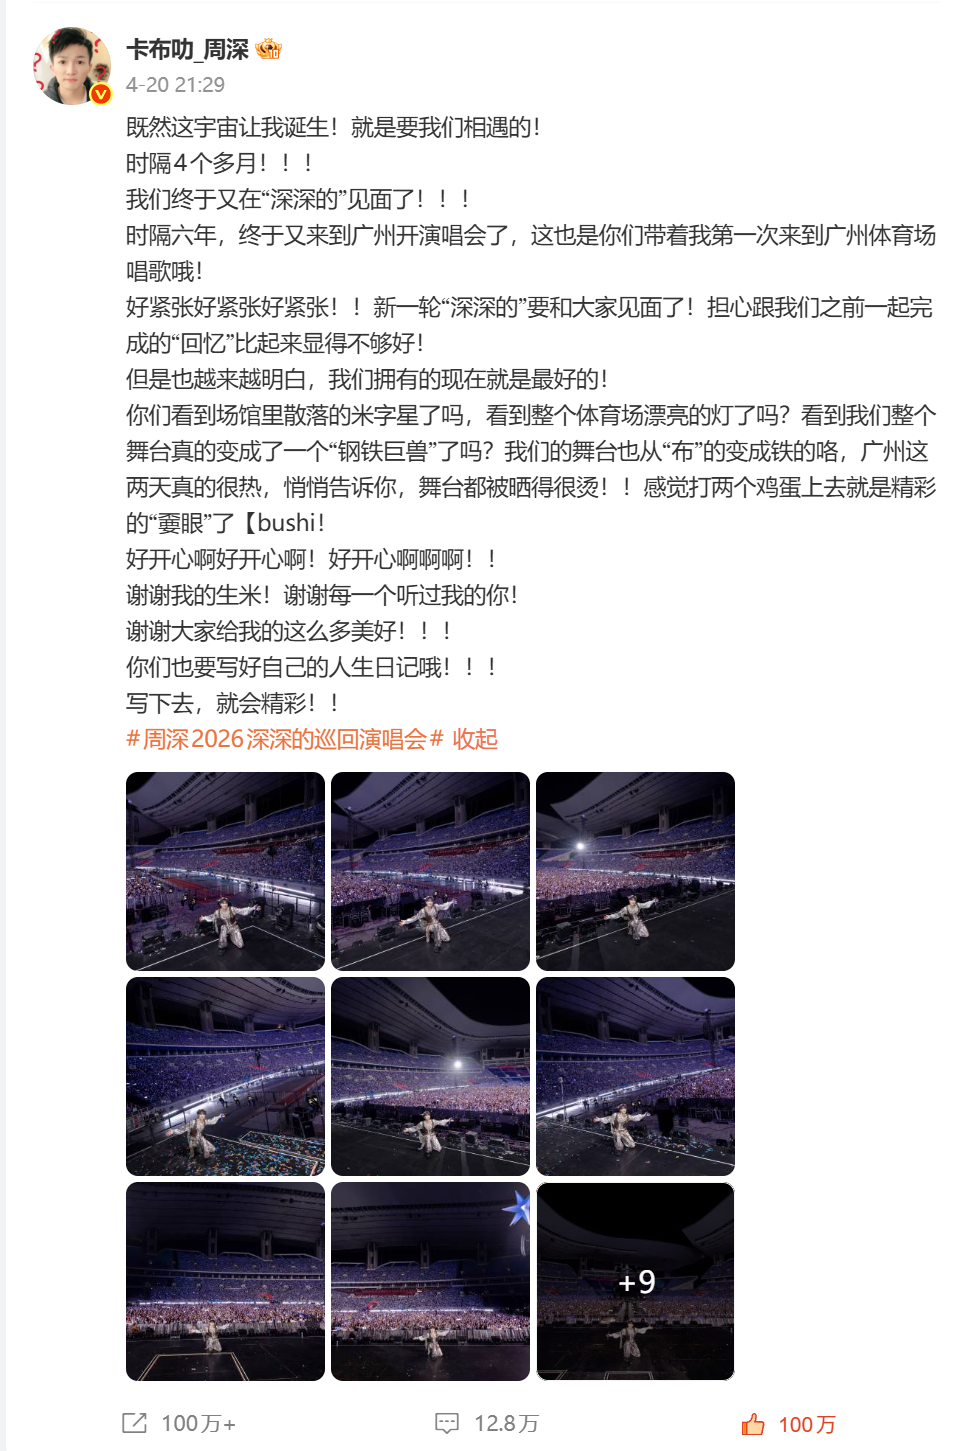
\includegraphics[width=280pt]{img/weibo/GuangZhou} 

}

\caption{周深2026.04.19广州场微博}\label{fig:unnamed-chunk-8}
\end{figure}

\newpage

\section{整理备注（待人工校对，终稿时删除）}\label{ux6574ux7406ux5907ux6ce8ux5f85ux4ebaux5de5ux6821ux5bf9ux7ec8ux7a3fux65f6ux5220ux9664-1}

\begin{enumerate}
\def\labelenumi{\arabic{enumi}.}
\tightlist
\item
  \textbf{录音来源}：002\_2026深深的\_广州0419\_内场1699\_合声版.mp3（约181分30秒，内场合声版）。整理方法同 SOP：37段×5分钟分段多模态转写，唱词对照《appendixG-2026歌词.Rmd》校正，口号互动逐轮记录，低置信处标〔听写待核〕；对组曲分界、串烧、末段等存疑处做了定点复核，末段（谢幕BGM）初转写内容经复核确认为幻觉已删除。
\item
  \textbf{本场定位}：2026年''深深的''巡演第2场（广州 Day2），广州城市末场（按规则在文末插入微博截图 R 块，图片待人工提供）。卷首语取小美满段''你们的出现，就是周深最好的陪伴''。本场城市限定粤语歌为《真的爱你》（Day1 为《一生所爱》，本场再现其副歌并调侃观众忘词）。广州 Day2 结构差异已落实：Part4 开场为吉量块（春雪），和光同尘块移至点歌后。
\item
  \textbf{关键时间点（按5分钟分段定位）}：开场VCR 00:00；修星星的人 约02:20；Try Everything 约06:25；问候+粤语环节 约10:20；光亮 约13:05（苏轼段约15:00）；若梦 约17:55（``提前让开''约20:40）；浮光 约21:35；借过一下 约26:10（``我找到你们了''约31:30）；机器人VCR 约31:30；请我不改 约33:50；Wala li longla口号+警报 约35:00--40:00（逐词递进教学约39:40）；来啊 约40:35；随机采访 约41:55；荧光棒游戏 约42:30；达拉崩吧 约46:30（Polo衫梗约45:30）；反深代词+蜃楼VCR 约51:35；天堂岛之歌 约52:55；记忆商店说白 约55:10；梦见你 约55:45；荒城渡 约57:45；人是\_ 约60:00；音乐动画VCR 约61:25；化身孤岛的鲸 约62:00（墙头科普约70:00）；花开忘忧 约71:15（老师感言约74:45）；粤语感想+《一生所爱》再现 约75:30；真的爱你 约77:15；小美满 约81:55（许愿约84:50）；总有美好在路上 约86:50；灯火里的中国 约88:05；我担介绍+独上西楼 约91:50；小城故事 约93:50；路边的野花不要采 约95:00；我只在乎你 约96:30；面具VCR 约99:10；吉量 约101:15；想见到气血满满的你 约103:20；春雪 约106:25；少管我 约107:45；奇迹时刻 约112:45（``昨天坏了的那个''梗约112:50；魔术约115:30，笔+红球两段，本场均成功）；好运来 约117:10；接财运 约121:00；点歌环节 约122:00（``一滴水''梗约122:50）；点歌小明 约123:30；重启 约128:10；点歌塔塔 约130:30；分分钟需要你 约133:35；和光同尘 约135:35；云裳羽衣曲 约136:30；怜悯 约138:30；望 约139:30；璀璨冒险人 约140:00；周可可/周嫑嫑 约144:20；致谢 约145:05（``靠谱''应答约149:40）；大合照 约150:00；我以渺小爱你 约153:35；交换日记VCR 约160:00；起风了 约162:55（``以爱之名''约167:00）；大鱼 约168:25；地球没有你 约174:55（告别大合唱至约180:00，谢幕BGM至录音结束约181:30）。
\item
  \textbf{点歌观众}：第一位小明（录音听作''小偶明''〔待核〕，汕尾人，B站UP主时期经九语版《Let It Go》认识周深，未出道前已听；现场清唱粤语版 Let It Go 片段；自称代表''南米群''〔待核〕点《重启》，带话''工作固然重要，但你也要好好照顾好自己''；自述I人、最大胆的事是来看演唱会、与刚认识的两位朋友同行）。第二位塔塔（录音听作''西塔/塔塔''〔待核〕，广西人，恰逢''三月三''假期专程来看演唱会；与周深山歌互动''唱山歌咧～这边唱来那边和～``；入坑曲《雪落下的声音》〔节目名听作''宫廷背包客''，待核〕；点《分分钟需要你》并称''就是想听你唱粤语歌''）。
\item
  \textbf{VCR 差异}：开场、机器人、面具、交换日记四段 VCR 与《appendixD》一致；机器人 VCR 开篇日期句''二二二五年五月十七日''与附录 D 一致；面具 VCR 开篇日期行本场为''2026年4月19日，广州''；蜃楼 VCR（天堂岛之歌前）本场听作周深配音''救我！这是哪里？``，观众齐答''你心里！``；音乐动画 VCR 结尾旁白本场听作''回忆虽然美好，但是因为有了你，我们更要继续往前行，对不对？``〔与0418场听作''如果遇到了你，我们一定可以好好享受现在。挣脱才能定义的束缚''不同，两句均待核，建议对照官方视频后择一补入附录D〕；交换日记 VCR''就会有精彩的篇章''（附录 D 作''新的彩页''，与附录 D 备注互证）。
\item
  \textbf{《地球没有你》现场改编版}：与 0418 首演改编版一致（``陪我，再走一公里，再听一首歌曲，准备这场别离''等）；本场个别句有出入待核：``害怕差一毫厘，就会错过你''（0418 作''害怕差一毫厘''同）、``爱你，是场感动又美丽的旅行''（0418 作''感动又愧对''）、``我会当成整个世界去经历''句。
\item
  \textbf{团队名单}：致谢名单与 0418 场及常州终版一致（出品周深工作室、时代立方；承办坚实文化；制作必应；总导演周佑洋、庄惟惞；音响工程南京奥斯泰；调音乐尔工作室〔本场录音听作''乐耳''，按 2026-11-17 已确认规范写法〕；服装劳伦斯许工作室、Third Studio、Windowsen；硬体北京立超舞台集团；票务大麦/猫眼/票星球）。本场特色：票务致谢时观众齐喊''靠谱！``（常州场为''倒闭！``）；金少刚老师''十件Polo衫/十个颜色/十全十美''梗；``第一次出道的舞台就是跟金少刚老师合作的''表述〔待核〕。
\item
  \textbf{听写存疑}：粤语问候段若干句（``你讲，得唔得啊''``系喔，你都系呢个人人生当中最靓嘅仔咯''``他们换衣服也这么的仓促''）；记忆商店''也就是米子和周星星''〔疑为''米子和周深深''或昵称玩笑〕；记忆商店演唱部分歌词；歌唱段间两次观众合唱句（两轮听写分别为''我说等没有等，没人记得''与''无数个没有你的季节''）；独上西楼现挂''这一颗，心的歌声，又是你的墙头''；吉量段''迎光吧''（疑为''荧光棒''）；``我的爪子穿成这样合理吗''；周嫑嫑平底锅''绵羊的衣服''句；致谢''合唱老师们/和声老师们''；接财运''我接个大舞台''合唱句；起风了''你还愿意相遇吗''；小明名字''小偶明''与''南米群''；塔塔名字''西塔''与《宫廷背包客》；粤语版 Let It Go 片段；谢幕BGM跟唱词句。另：借过一下收尾段初转写''白光隐藏\ldots\ldots``数句与已知歌词不匹配，判为识别噪声未收录。
\item
  \textbf{唱词校正说明}：正文唱词均按《appendixG-2026歌词.Rmd》校正，主要修正同 0418；本场特有：吉量''高高山上鸾鸟唱/东海浪里搅银汤/建木树下唤吉量''；璀璨冒险人Rap段''没人未梦就先懂''按附录校正；小城故事城市现挂''广州故事多/若是你到广州来/广州来做客''；路边的野花''墙头多的人听到喽''现场改词。
\item
  \textbf{待补充}：歌单图（img/playlists/GuangZhou-20260419.png）及现场图片待插入；广州城市告别微博截图（img/weibo/GuangZhou.png）待人工保存提供，R 块已按城市末场规则插入。
\end{enumerate}

\chapter{2026.05.02武汉场 (WIP)}\label{WuHan-20260502}

\begin{quote}
谢谢你们选择来跟我相遇，谢谢这个宇宙让你们诞生了。------周深
\end{quote}

\begin{figure}

{\centering 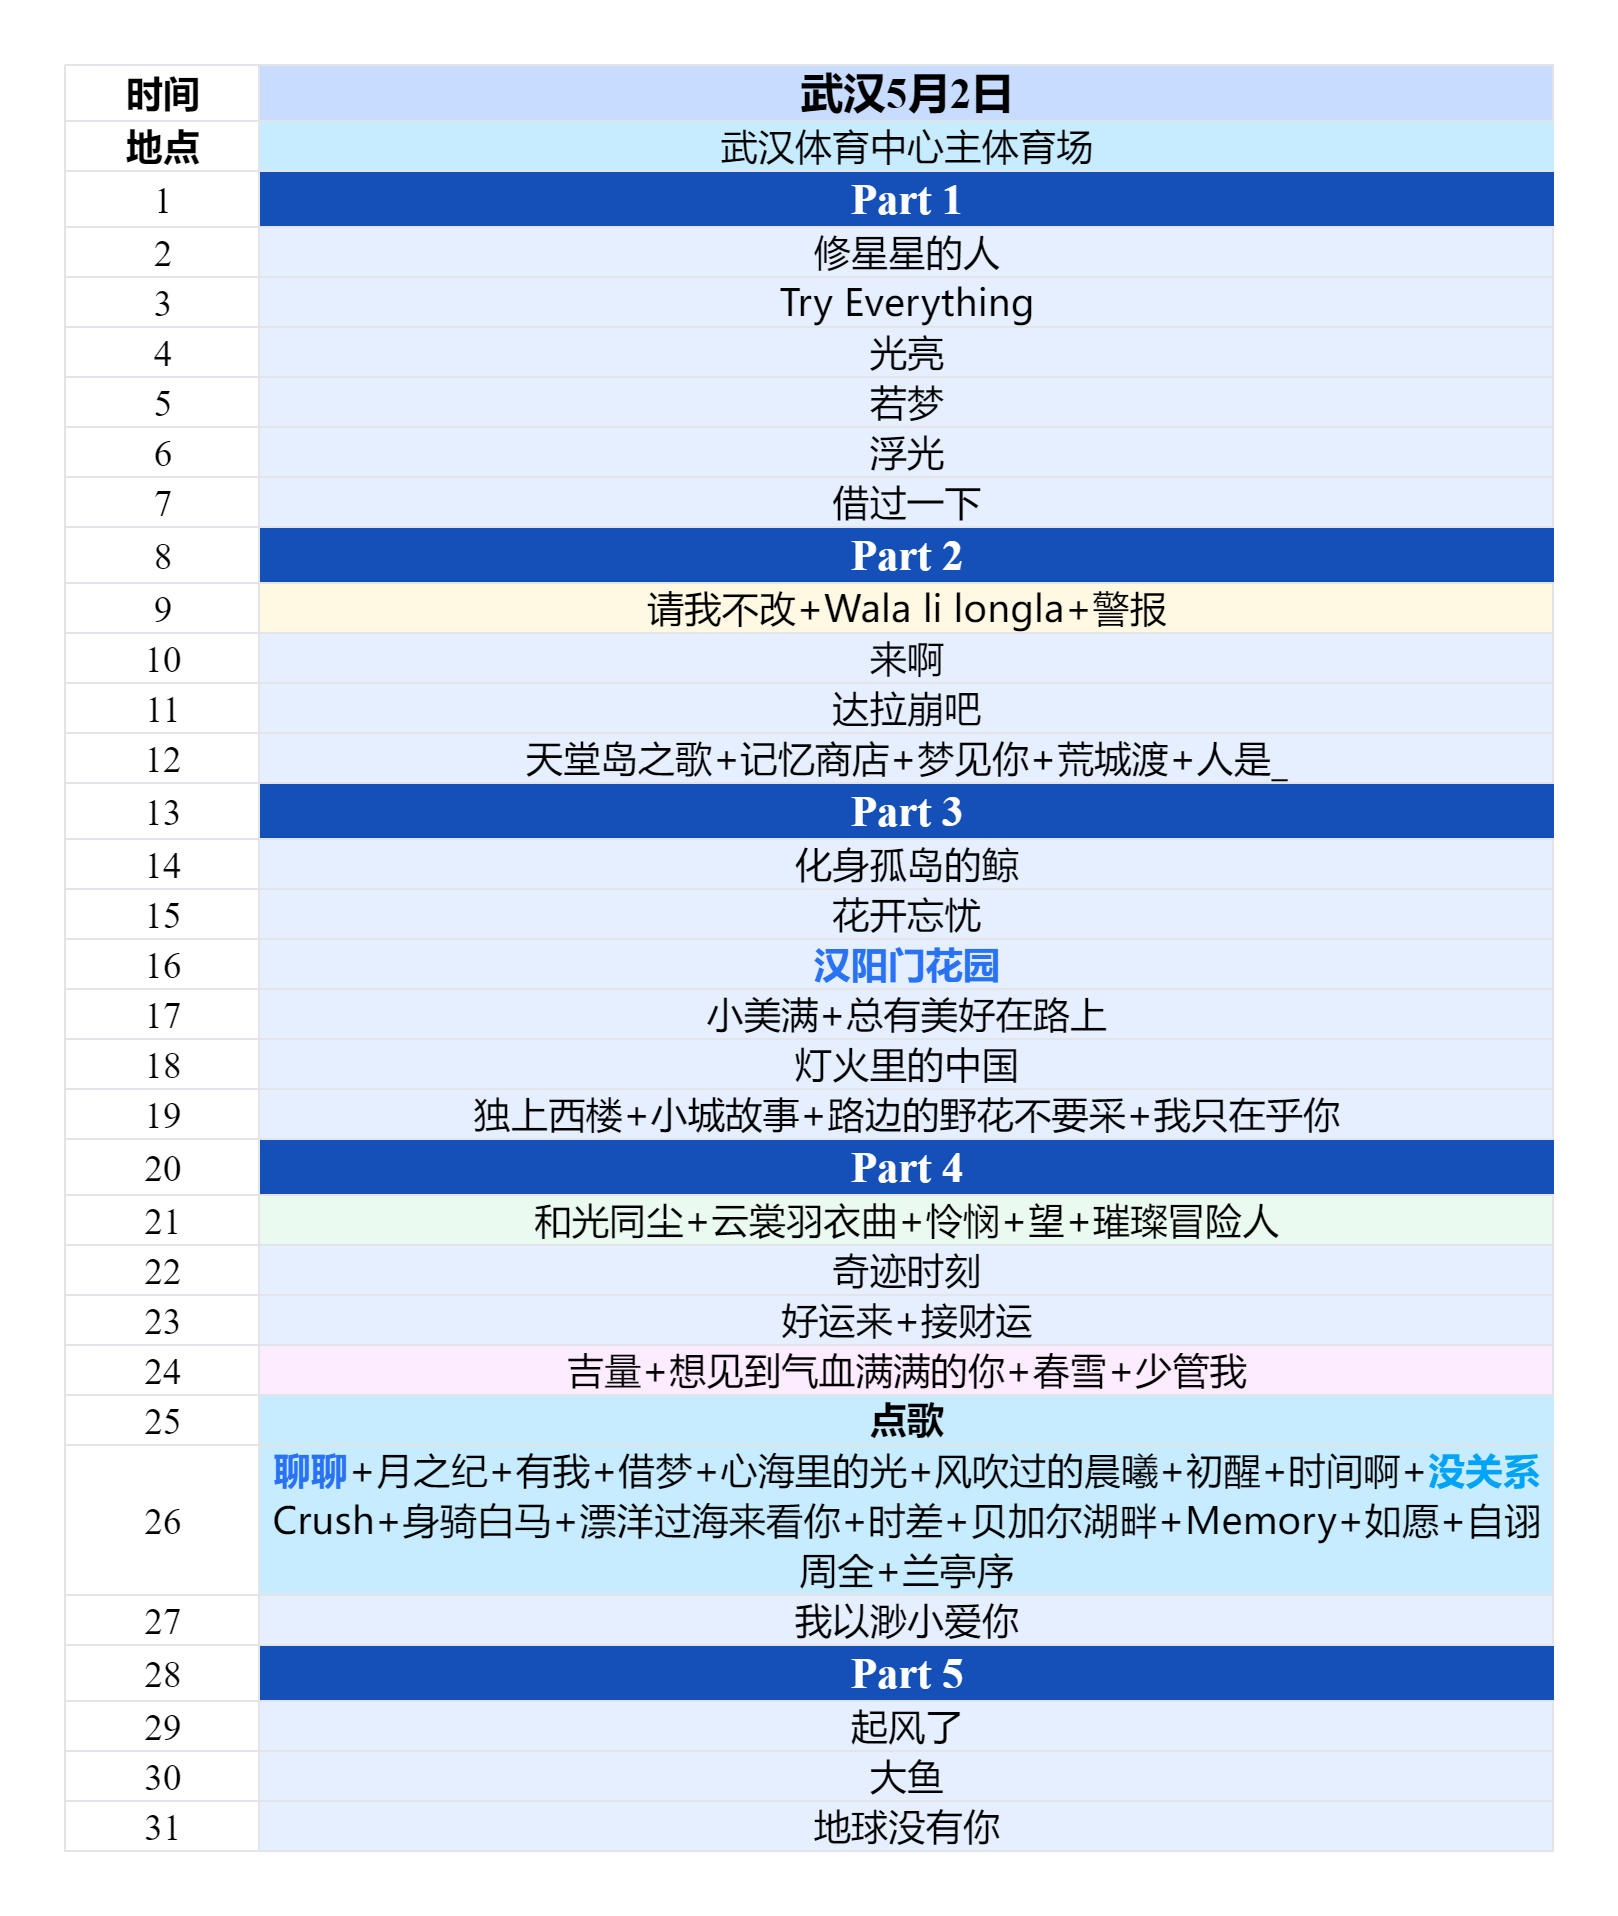
\includegraphics[width=280pt]{img/playlists/WuHan-20260502} 

}

\caption{2026周深“深深的”巡回演唱会2026.05.02武汉场歌单}\label{fig:unnamed-chunk-10}
\end{figure}

\newpage

\section{Part1}\label{WuHan-20260502-part1}

\hyperref[opening-vcr]{🎥【\textbf{开场VCR}】}

\hyperref[xiu-xing-xing-de-ren]{🎵【\textbf{修星星的人}】}（深：既然这宇宙让我诞生\ldots\ldots 我的情感和三十六度的体温，足以暖热即将熄灭的恒星\ldots\ldots 在时间的深海里，给地球道一声晚安〔或作''给武汉道一声晚安''，按1107场惯例待核〕）。武汉的朋友们，你们好吗？（米：好------！）后面的朋友！（米：欢呼声）让我听到你诞生的声音！（米：啊------！）。

\hyperref[try-everything]{🎵【\textbf{Try Everything}】}既然宇宙让我诞生了，我们就好好的相遇好不好？（米：好------！）（深：I messed up tonight, I lost another fight\ldots\ldots I wanna try even though I could fail\ldots\ldots Oh oh oh oh oh，Try everything）尖叫声！（米：啊------！）（深：你们来！）（米：Try everything）（深：你们！）（米：Try everything）（深：再大声！）（米：Try everything）你们也要记住，Try Everything好吗？（米：好！）。

  哇，武汉的朋友们，周深的巡回演唱会又来了，你们准备好了吗？（米：准备好了！）这是我\ldots\ldots 哎，第二次来武汉开体育场演唱会。这都是谁创造的奇迹呀？（米：你！周深！）这个答案是我们！（米：是的！）好不好？然后来到了武汉，肯定要说几句武汉话。武汉的朋友们，大家好！我是周深。蛮开心又在武汉跟大家见面了。你们吃了冇？（米：吃了！）有没有人没吃东西啊？（米：没有！）有的话那就散了散了。看完演唱\ldots\ldots 哎这句不会说。看完演唱会我们再回去好好吃好不好？（米：好！）后面的朋友你们好吗？（米：好！）哇，让我听一下武汉场第一场的声音有多大？（米：欢呼声）谢谢每一个修星星的你，是你们才让这一切发生，是你们才让这一切的灯光亮起。你们也千万不要忘记，你们身上一直在发光好吗？（米：好！）谢谢你们愿意来跟我们见面，好开心啊。哎，现在没有下雨哎。（米：欢呼声）那是因为你们出现了，你们知道吗？（米：因为你！）还是有点害羞不好意思大喊。（米：知道！）但是呀，请你们一定要确信，你们的出现就是我的光亮。

\hyperref[silver-linings]{🎵【\textbf{光亮}】}宝你们的头。（米：宝贝！宝贝！宝贝！）后面的朋友。（深：海上一阵风吹起，白云涌向陆地\ldots\ldots 也许你猜不透未知的宿命\ldots\ldots）可是啊我却，（米：我却愿意相信）最渺小最微弱最柔软最无畏的你。（深：用尽了全力，努力地去回应，再无边再无尽再无解总有一线生机）交给你们。（米：照亮你自己）。（深：光亮你自己）我爱你们！（米：欢呼声）（深：莫听穿林打叶声，何妨吟啸且徐行。竹杖芒鞋轻胜马，谁怕？一蓑烟雨任平生\ldots\ldots 六百年一粟，沧海一梦）谢谢你们每一个人！

\hyperref[like-a-dream]{🎵【\textbf{若梦}】}谢谢你们，美好的，就像一场梦一样。等一下大声一起唱好吗？（米：好！）（米：宝贝！宝贝！）（深：浮生若梦，为欢几何\ldots\ldots 看天地之间皆漠漠）到你们了。（米：往事流转在你眼眸）后面的朋友。（深：一边遗忘，一边拼凑）（深：如果虔诚，合十双手，唯愿你能得到拯救）被你们听见，我就得到拯救啦。（米：欢呼声）那边的朋友！（米：往事流转在你眼眸）（深：一边遗忘，一边拼凑）再大声！（米：如我虔诚，合十双手，唯愿你能得到拯救）交给你们！全场最大声！（米：往事流转在你眼眸）后面的朋友！（深：在你眼眸）（米：一边遗忘，一边拼凑）（深：一边拼凑）（米：如我虔诚，合十双手）（深：合十双手，唯愿你能，得到拯救）（深：因为你们，我才得到拯救）也有你啦。〔``也有你啦''一句听写待核〕

\hyperref[floating-light]{🎵【\textbf{浮光}】}（旁白〔疑似视频或口白，归属待核〕：人生恍惚三万天，因为遇见你，才值得留恋哦。）（深：看指尖拨响蝴蝶，扇动一场离别。我推开无声岁月，续梦一页\ldots\ldots 你的眼眸装满了时间，你的身后拥故事成篇，此生如梦愿细数流年，与你同写沧海桑田）（深：你说那月光，照过同样城墙\ldots\ldots 这是我也是你，不曾遗忘的啊）（米：浮光掠影重山彩云间，你的伏线穿越千百年，人生不过恍惚三万天，漫漫人间，留恋流连）。

\hyperref[excuse-me]{🎵【\textbf{借过一下}】}哇，好像你们不知道这一首歌在唱什么一样。〔玩笑，语境听写待核〕（深：少年扬起脸庞，前往他的月亮\ldots\ldots 你们都是对的，他说拜托，让开一下）（深：潇洒不是不怕，是愿付出代价）你们愿意吗？（米：愿意！）（深：权衡利弊后，仍守对与错，谢过赐教的话，路借过一下）武汉的朋友准备好大合唱了吗？（米：啊------）（深：让我大醉一场，殿堂之上，背闲诗两三章）后面的朋友？（米：让我穿白衣裳，过疯人巷，去泥潭捞月光）太大声了，好。〔现场反应，待核〕（深：望大人们见谅，提点的话，我懂也不想装，世人寻黄金乡，我找月亮，何必同往）（深：话谢过，路借过，你是你，我是我）\textbf{\textcolor{red}{我爱你们}}！（深：人见过明暗，若天真犹在，当披上月光，走夜晚）你们，就是我要找的月光。谢谢你们。（米：欢呼、尖叫）

\section{Part2}\label{WuHan-20260502-part2}

\hyperref[robot-vcr]{🎥【\textbf{机器人VCR}】}

\hyperref[brave-heart]{🎵【\textbf{请我不改}】}武汉的朋友们好吗？（米：好！）晚安！（米：晚安！）你们！（米：我爱你！）晚安你！（米：晚安你！）晚安你！（米：晚安你！）晚安！（米：晚安！）晚安你！（米：晚安你！）晚安你！（米：晚安你！）晚安你！（米：晚安你！）晚安你！（米：晚安你！）（深：是谁在我耳边念白\ldots\ldots 是谁模糊我的未来，恐惧淹没了期待。绝望已经大军压境，回身却没半个人影，才看清追兵与逃兵，竟都是我自己〔开场两三句听写不清，待核〕）尖叫声！（米：啊------！）（深：请我不改，我的姿态，我的爱我的痛都与生俱来\ldots\ldots 放肆盛开）（深：Brave heart）嘿！（米：嘿！）（深：我存在）嘿！（米：嘿！）\ldots\ldots{}

\hyperref[wala-li-longla]{🎵【\textbf{Wala li longla}】}（与《请我不改》《警报》连唱串烧）我此生快活呐！〔现场唱词，待核〕哇啦！（米：哇啦！）哇啦哩！（米：哇啦哩！）哇啦哩噜！（米：哇啦哩噜！）全场！（米：哇啦哩隆哒！）（深：\ldots\ldots 转身就走〔串烧段唱词听写不清，待核〕）（深：请我不改，我的姿态\ldots\ldots 坦荡痛快）哇啦！（米：哇啦！）最大声！哇啦哩！（米：哇啦哩！）哇啦哩噜！（米：哇啦哩噜！）哇啦哩隆哒！（米：哇啦哩隆哒！）（深：\ldots\ldots 我只会痛，为你而痛〔唱词待核〕）哇啦！（米：哇啦！）哇啦哩！（米：哇啦哩！）哇啦哩噜！（米：哇啦哩噜！）哇啦哩隆哒！（米：哇啦哩隆哒！）（米：啊------！）他们的舞蹈动作其实设计的不是这样的。而是因为这首歌跳完太累了。他们是发自内心加的这个动作。那我想听到全场最大声的''哇啦哩隆哒''！（米：哇啦哩隆哒！）声音很好，很大声。武汉的朋友们你们太棒了！

\hyperref[jing-bao]{🎵【\textbf{警报}】}（深：\ldots\ldots 这结果，到底有，多汹涌，到不如转身就走\ldots\ldots 为你而痛）〔本段嵌入《请我不改》串烧中，唱词整段听写待核〕

\hyperref[lai-a]{🎵【\textbf{来啊}】}那准备好唱下面这首《来啊》了吗？（米：啊------！）我教你们一下啊。（深：Don't tell me lie, lie）会了吗？（米：会了！）试一下啊。（深：Don't tell me lie, lie）这边。（深：Don't tell me lie, lie）起了吗？后面的朋友起了吗？（米：起了！）不会最后我会发现我这句话特别不标准吧。〔语境待核〕但不管怎么样，来呀。〔口头沿用''来呀''，曲名作《来啊》〕（深：我怎么就这样呆头呆脑，一不小心落入圈套\ldots\ldots 天生的怪胎\ldots\ldots 别气急败坏，别着急淘汰，一万种防备阻碍，不如就算了，靠过来。将错就错，别拖Let's go，随你操控）（深：Don't tell me lie eeeee，Lie eeee，我望眼欲穿你别闪躲）再来。（深：Don't tell me lie eeeee，Lie eeee，要爱就爱放纵吧别退缩）\textbf{\textcolor{red}{我爱你们}}！（深：Don't tell me lie eeeee，Lie eeee，我倾其所有赴汤蹈火\ldots\ldots 敢不敢直视我，Let's fall）谢谢。武汉的朋友们你们真的太棒了！好热情啊，真的欢呼声好大，是我的错觉吗？（米：不是！）后面的朋友们呢？（米：欢呼）

  谢谢。那接下来到了我们深深的巡回演唱会的小游戏环节了。每个人的荧光棒可以自己选择你喜欢的颜色，分别是蓝色、黄色、粉色和绿色。然后每个不同的颜色它都代表着不同的角色。希望大家选一下自己喜欢的颜色和想成为的角色。那无论如何你们都是自己人生\ldots\ldots 完全没有人在听我说话。同学们你们好吗？（米：好！）无论选择什么颜色，你们都是自己人生当中的------（米：角色！）好，给大家五秒钟的时间选择你们喜欢的颜色哟。蓝色代表的是达拉崩吧。黄色代表的是国王陛下。粉色是\ldots\ldots 你们过来一下，衣服稍微有点紧。〔对伴舞/工作人员，待核〕粉色是公主米娅。昨天试的时候也没有这么紧。绿色是谁？（米：恶龙！）恶龙我们今天改一下，要不你''七了冇''好不好？〔武汉话''吃了冇''，听写待核〕不了不了。这样，那相应的角色都有他们自己的台词，所以等一下我喊到谁的名字，你们就要喊出你们的台词好不好？（米：好！）试一下啊。达拉崩吧。（米：我最棒！）国王陛下。（米：再说一次！）公主米娅。（米：救我！）恶龙。（米：嗷呜！）一看就是有很多朋友不是第一次来到我们演唱会，他选择了红色。没事，红色我就喊武汉，你们喊''七了冇''〔听写待核〕，好不好？（米：好！）宝贝。你们没有其他选择，宝你们个头。试一下啊。武汉！（米：宝贝！）哦，最后这句话变成宝贝了吗？〔听写待核〕宝你们个头。达拉崩吧。（米：我最棒！）国王陛下。（米：再说一次！）公主米娅。（米：救我啊！）恶龙。（米：嗷呜！）达拉崩吧。（米：我最棒！）国王陛下。（米：再说一次！）公主米娅。（米：救我啊！）恶龙。（米：嗷呜！）达拉崩吧。（米：我最棒！）国王陛下。（米：再说一次！）国王陛下。（米：再说一次！）国王陛下。（米：再说一次！）恶龙。（米：嗷呜！）达拉崩吧。（米：我最棒！）恶龙。（米：嗷呜！）国王陛下。（米：再说一次！）公主米娅。（米：救我啊！）公主米娅。（米：救我啊！）恶龙乘以十。（米：欢呼）武汉乘以五。（米：宝贝！宝贝！宝贝！宝贝！宝贝！）把你们那个求你们的说一下〔听写不清，待核〕。武汉。（米：宝贝！）我们一起来。好过分。我们一起来演唱这首《达拉崩吧》好不好？（米：好！）

\hyperref[dalabengba]{🎵【\textbf{达拉崩吧}】}（深：很久很久以前，巨龙突然出现，带来灾难，带走了公主又消失不见\ldots\ldots 他说，陛下我叫，达拉崩吧斑得贝迪卜多比鲁翁，再说一次，达拉崩吧斑得贝迪卜多比鲁翁。是不是，达拉崩吧斑得贝迪卜多比鲁翁？对对，达拉崩吧斑得贝迪卜多比鲁翁）全场。达拉崩吧。（米：我最棒！）国王陛下。（米：再说一次！）公主米娅。（米：救我啊！）恶龙。（米：嗷呜！）达拉崩吧。（米：我最棒！）国王陛下。（米：再说一次！）公主米娅。（米：救我啊！）恶龙。（米：嗷呜！）（深：英雄达拉崩吧，骑上最快的马，带着大家的希望，从城堡里出发\ldots\ldots 巨龙说，我是昆图库塔卡提考特苏瓦西拉松，再来一次，昆图库塔卡提考特苏瓦西拉松。是不是，昆特牌提琴烤蛋挞苏打马拉松？不对是，昆图库塔卡提考特苏瓦西拉松）达拉崩吧。（米：我最棒！）国王陛下。（米：再说一次！）公主米娅。（米：救我啊！）恶龙。（米：嗷呜！）武汉。（米：宝贝！）达拉崩吧。（米：我最棒！）全场。于是。（米：达拉崩吧斑得贝迪卜多比鲁翁，他战胜了昆图库塔卡提考特苏瓦西拉松，救出了公主米娅莫拉苏娜丹妮谢莉红，回到了蒙达鲁克硫斯伯古比奇巴勒城〔合唱串词，待核〕）后面呢？（米：达拉崩吧斑得贝迪卜多比鲁翁，他战胜了\ldots\ldots）哎呀，好了。（米：达拉崩吧斑得贝迪卜多比鲁翁\ldots\ldots）后面呢？（米：最后达拉崩吧斑得贝迪卜多比鲁翁\ldots\ldots）全场。（米：从此达拉崩吧斑得贝迪卜多比鲁翁，跟达拉崩吧斑得贝迪卜多比鲁翁，还有昆图库塔卡提考特苏瓦西拉松，还有公主米娅莫拉苏娜丹妮谢莉红\ldots\ldots 还有他们生下一个\ldots\ldots〔结尾大串烧合唱，听写待核〕）达拉崩吧！（米：我最棒！）阿木。〔应答内容听写待核〕（米：为你变出小仙女，不谢儿子〔听写不清，待核〕）阿木是大制作呀！〔待核〕（米：大制作！）阿木。〔待核〕（米：大制作！）公主米娅。（米：啊！）恶龙。（米：嗷！）武汉。（米：宝贝！）宝贝！他的全名十分难念，要念你来念吧〔位置按过门归属，待核〕。武汉。（米：宝贝！）过分。

  那接下来这个串烧，让我们去看一下，我前年发的专辑叫做------（米：反身代词！〔现场应答即《反深代词》之常见误听〕）武汉。（米：宝贝！）前年没有发这张专辑。〔玩笑，听写待核〕《反深代词》世界有一栋蜃楼，在去年深深的巡回演唱会的时候，有人被困在蜃楼里出不来了。那接下来发生了什么事情呢？我们一起来看一下好不好？（米：好！）（米：宝贝！宝贝！）

\hyperref[haven-song]{🎵【\textbf{天堂岛之歌}】}（深：叮咚，我有一个秘密，悄悄告诉你，欢迎你来到天堂入口\ldots\ldots 叮咚，有人在看你的过去，我逃不出去）生米们在哪里？〔听作''小米在哪里''，按惯例校，待核〕（米：在这里！）
\hyperref[the-memory-store]{🎵【\textbf{记忆商店}】}（合唱：我可以送你回家吗\ldots\ldots〔本段唱词听写不清，待核〕）哦，这是《反深代词》世界当中的记忆商店。哦，只要拥有了这一颗米子心，我们就可以唤醒并且购买我们最喜欢的那一段回忆。〔听写含''吃螺蛳粉''一段，为误听，已按1107场惯例删除，待核〕啊，米子心。（米：哇！）
\hyperref[meng-jian-ni]{🎵【\textbf{梦见你}】}（深：看着眼前，还年少的你，恍如流年从没淌过去\ldots\ldots 若多年后还能够有幸，重逢在另一场梦境，但愿那时你在人海里，仍将我一眼认清）（米：不朽的永恒的，我们记得〔听作''无数的没有了没人记得''，按1107场BGM惯例校，待核〕）〔同句重复一轮〕非要跑那么远，跑远了也累。〔对舞台装置/演员，语境待核〕
\hyperref[huang-cheng-du]{🎵【\textbf{荒城渡}】}（深：夜色中寻觅过，当往事困住我，也盼心中生出一点萤火\ldots\ldots 断了这心魔，可原谅我，宿命中获得这解脱，重来过。眼中拂尘，手中残魂，那故事斑驳荒城\ldots\ldots 握一颗糖暖这孤身颠簸）。
\hyperref[Humans_are_]{🎵【\textbf{人是\_}】}（深：未知摊开棋局，舍弃昨日才可破，再见了我的月光，我的蓝，我的爱\ldots\ldots 让死亡觊觎我，让恐惧亲吻我，来摧毁我深爱的一切，可仍夺不走我的选择。弹指间湮灭我，但命运打不败活着。是微茫中高歌的族类，生命像烟火那就点亮，孩童的双眸，未来的瞳孔）。

  既然这宇宙让我们诞生，我们要好好珍惜彼此，好好相遇好不好？（米：好！）谢谢你。是因为遇见了你，才让我们都不再被回忆困住。我们现在才是拥有最好的东西，你们说对不对？（米：对！）（深、米：不朽的永恒的，我们记得）〔同句共三轮〕（深：高音吟唱）（米：欢呼、尖叫）〔本段后有彩带与字条落下，观众席议论未收录〕

\section{Part3}\label{WuHan-20260502-part3}

\hyperref[music-animations-vcr]{🎥【\textbf{音乐动画VCR}】}

\hyperref[The-whale-who-became-an-island]{🎵【\textbf{化身孤岛的鲸}】}武汉的朋友们！（米：在！）让我听到你们的声音好不好？（米：好！）（深：我是只化身孤岛的鲸，有着最巨大的身影\ldots\ldots 你的衣衫破旧，而歌声却温柔，陪我漫无目的的四处漂流\ldots\ldots 我想给你能奔跑的岸头）（米：没有！没有墙头！）谢谢每一个听到我、看到我最美好的你们。（米：我爱你！）但是呀，你们有多少个墙头呢？（米：没有！没有墙头！）我才不信你们没有墙头。（米：有！）你们居然还敢说你们没有墙头。（米：没有墙头！）墙头有多少？我解释一下，墙头的意思啊就是说每次问，每次哎，你们喜欢哪个歌手啊？（米：周深！）但是他们其实喜欢超级多个歌手。那我们就暂时不礼貌的把他们称为墙头。但是我又怎么样？你们都是我的国王和王后。

\hyperref[Blossoms-that-forget-sorrow]{🎵【\textbf{花开忘忧}】}我们来武汉看你咯。你有没有好好照顾好自己呀？（米：有！）声音不够大。好好照顾好自己好不好？（米：好！）（深：巷子口买了花，穿过沿街红墙青瓦\ldots\ldots 一件遗憾的事，就喝一碗汤，庭院深深，秋叶飘落）（深：若记忆被偷走了，忘了我的爱，我会说）说什么？（米：你好！）你们好吗？（米：好！）（深：这是给你的花，花的名字叫忘忧草。它说时光汹涌，如水上烟波，别走远了一起回家）我们来武汉看你们咯！谢谢每一个创造奇迹的你。（深：我们苍老的时候就回到小时候\ldots\ldots 捡了小猫名为苍狗）（深：你好啊，离开的人啊，请帮我相爱到剧终。忘忧草开着花，你在月光下不说话，一件遗憾的事就喝一杯茶，庭院深深，秋叶飘落）。

  在我们的人生当中，一定有那一个对你非常非常重要的人。但是我们也有很多很多的遗憾，跟他没有办法再一次见面。请相信我们的思念他一定听得见，对不对？（米：对！）一定要好好照顾好自己，因为他们也一定都看得见，对不对？（米：对！）花开忘忧，愿你无忧。（米：愿你无忧。）花开忘忧。（米：愿你无忧。）谢谢你们。（米：谢谢周深！）

  啊，既然我们来到了武汉，而且武汉对我来说它非常非常的特别，因为是我出道之后第一次以歌手周深，然后进行的第一场演出就是在武汉。所以武汉的朋友们，一看就是只学了''武汉的''这三个字。我，歌手周深又回来啦！（米：欢呼声）是你们为我点亮了一盏又一盏的灯，所以千万不要小瞧你们自己好吗？（米：好！）这一切都是你们为我创造的奇迹哟。上一次来武汉的时候演唱的是生日快乐歌。那这一次终于可以唱一唱我们非常有本地特色的歌曲，《汉阳门花园》有人会唱吗？（米：不会。）哦，那看来有很多外地的朋友是不是？（米：是！）那我们外地来玩的朋友喜欢武汉吗？（米：喜欢！）我们来听一首特别有乡愁、有韵味的这一首歌，《汉阳门花园》，会唱的等下跟我一起唱好不好？（米：好！）让我看到你的荧光棒。

\hyperref[han-yang-men-hua-yuan]{🎵【\textbf{汉阳门花园}】}（深：小时候的民主路冇得那多人，外地人为了看大桥才来到汉阳门。汉阳门的轮渡可以坐船去汉口，汉阳门的花园，属于我们这些住家的人。冬天腊梅花，夏天石榴花，晴天都是人，雨天都是伢\ldots\ldots 现在的民主路每天都人挨人，外地人去了户部巷就来到汉阳门\ldots\ldots 小小这座城，等你回家的人。几年冇回家，天天都想家家，家家也每天在等到我，哪一天能回家。铫子煨的藕汤总是留到我一大碗，吃了饭就在花园里头等她的外孙伢）会唱的一起！（米：冬天腊梅花，夏天石榴花，晴天都是人，雨天都是伢）全场！（米：冬天腊梅花，夏天石榴花）你们！（米：冬天腊梅花，夏天石榴花）（深：过路的看风景，住家的卖清茶）（米：过路的看风景，住家的卖清茶）（米：欢呼声）

\hyperref[simple-bliss]{🎵【\textbf{小美满}】}那这首歌愿意跟我一起大声唱吗？（米：愿意！）让我听到你的声音好不好？（米：好！）最大声哦！（深：没什么大愿望）唱！（米：没有什么事要赶\ldots\ldots 乌云还挺大胆，顶在头上吹不散，我抓在手里捏成棉花糖，什么烦恼不能忘）全场最大声！（深：你看小狗在叫，树叶会笑，风声在呢喃\ldots\ldots 不去想，不必想，不用急急忙忙说一个答案）谢谢你们的出现！（米：谢谢周深！）再来。（深：笑一笑就灿烂）怎么了？（米：唱一支歌就舒展〔或作''唱一句歌''，待核〕）收集一点一滴小美满，都是幸福的花样，没道理的开朗，唱！（米：打扮平凡的日常）\ldots\ldots 全场最大声！\ldots\ldots 谢谢武汉的朋友！（米：谢谢周深！）你们辛苦啦！

  来让我们一起在《小美满》这首歌当中许愿好不好？（米：好！）像我这样，闭上眼睛，然后想好你心中想要许的愿望。我喊321睁开眼睛，我们许的愿望就会出现在这棵许愿树上哦。请相信相信的力量，请相信你们所有人美好的力量。现场所有人闭上眼睛，想一想想要许的愿望哦。想一想每次生日的时候都想要许的愿望呢。哦，对了，在《小美满》这首歌当中的愿望有一个要求，只能够许关于自己的愿望。想一想，是不是很久没有好好照顾好自己了？是不是很久没有想一想，自己这一路走来已经非常非常棒了？想一想，是不是很久没有跟自己，或者是从来没有说过，你辛苦了。想想这个愿望，三二一，睁开眼睛。你们的愿望一定会实现的，对不对？（米：对！）（深：相信什么就把世界看成什么样\ldots\ldots 记得保管小小的光环。笑就好，哭也好，今天就是明天最好的陪伴。笑就好，哭也好，自己就是自己最好的陪伴）你们都是周深最好的陪伴。〔听作''你们都是就是最好的陪伴''，按1107场惯例校，待核〕一定一定要好好爱自己好吗？（米：好！）爱自己一定是终身浪漫的开始。你们说，对不对？（米：对！）

\hyperref[zong-you-mei-hao-zai-lu-shang]{🎵【\textbf{总有美好在路上}】}（深：花在开，云在飘，笑容在脸上，我们向前方一路向阳）全场最大声！（深：亲爱的你）（米：在路上慢慢逛，看一看太阳）（深：晚风轻轻吹拂你的脸庞）（米：今天过去，要到明天看看天气会怎样，雨或晴朗，故事都慢慢赏）抬头发现，（米：原来你就是光芒）（米：欢呼声）

\hyperref[deng-huo-li-de-zhong-guo]{🎵【\textbf{灯火里的中国}】}准备好一起唱出最美的《灯火里的中国》了吗？（米：准备好了！）是你们组成的哟。（深：都市的街巷已灯影婆娑\ldots\ldots 灯火里的中国青春婀娜，灯火里的中国胸怀辽阔，灯火漫卷的万里山河，初心换回了百年承诺）你们好啊！等一下让我听到你们最大的声音好不好？（米：好！）全场！（米：灯火里的中国，青春婀娜）再大声！（米：灯火里的中国，胸怀辽阔）太好听了！（米：灯火漫卷的万里山河，初心换回了百年承诺，灯火荡漾着心中的歌）（深：高音吟唱）全场！（米：灯火里的中国，青春婀娜）再大声！（米：灯火里的中国，胸怀辽阔。灯火灿烂的中国梦，灯火荡漾着心中的歌）（米：哇------）你们还有和声。〔现场对观众和声的调侃，待核〕（深：高音吟唱）（米：啊------）太好听了。真的太好听了。但是我只会这一句武汉话，吃了冇？（米：笑）我还想再听一句。〔现场互动，待核〕（深：灯火里的中国）（米：青春婀娜）（深：灯火里的中国）（米：胸怀辽阔）（深：灯火灿烂的中国梦）（米：灯火荡漾着心中的歌）（深：灯火）（米：荡漾着心中的歌）仔细听哦，居然还有和声，证明你们真的很没默契。〔``很没默契''或作''很有默契''，待核〕（深：心中）（米：的歌）朋友们，真的太好听了。谢谢你们！（米：谢谢周深！）不不不，真的是谢谢你们。谢谢你们的出现让我觉得，哇，原来有那么多人愿意来跟我见面，愿意来为我点亮那一束光。谢谢你们，千万不要忘记自己一直在发光好吗？（米：好！）请相信永远的坚信，你的存在就是最有意义的事情，好不好？（米：好！）

  那接下来呢又到了我在我演唱会上介绍我担的时刻了。我担的名字很多人应该都不陌生，邓丽君女士。她的歌非常好听，可以说她的歌里面有很多人的回忆吧，就像是时间胶囊一样。所以我也希望可以努力成为像她这样的歌手，去唱好多好多歌陪伴你们，成为你们的时间胶囊的制造者，好不好？（米：好！）后面的朋友们听到了吗？（米：听到了！）那等一下会唱的歌跟我一起大声唱好不好？（米：好！）

🎵【\textbf{邓丽君组曲}】
\hyperref[du-shang-xi-lou]{🎵【\textbf{独上西楼}】}（深：无言独上西楼，月如钩，寂寞梧桐，深院锁清秋。剪不断，理还乱，是离愁〔或按1107场惯例作''是你们的墙头''，听写待核〕）（米：没有离愁！〔应答内容待核〕）（深：别有一番滋味在心头）来！
\hyperref[xiao-cheng-gu-shi]{🎵【\textbf{小城故事}】}（深：小城故事多）怎么了？（米：〔待核〕）〔现场应答听写不清，待核〕（深：若是你到武汉来，〔现场改词，后句待核〕）怎么了？（米：〔待核〕）哎，跟我说一下，怎么啦？（米：〔待核〕）再来！（米：〔待核〕）（深：人生境界真善美，武汉已包括）谈的谈，说的说，你们谁的墙头多？（米：我没有！）（深：请你的朋友一起来，武汉来做客）（米：请你的朋友一起来，武汉来做客）
\hyperref[donot-pick-the-roadside-flowers]{🎵【\textbf{路边的野花不要采}】}这首歌会唱吗？（米：会！）让我听到最大的声音！（深：送你送到小村外，有句话儿要交代，虽说已经是百花开）那些墙头多的人啊，都听好了。（深：路边的野花）他怎么了？（米：不要采！）哎呀，可不是我说的哟。全场！（米：记着我的情，记着我的爱，记着有我天天在等待）（深：我在等着你回来）千万不要把我来忘怀，（米：千万不要把我来忘怀）（深：千万不要把我来忘怀）你们会忘了我吗？（米：不会！）
\hyperref[I-only-care-about-you]{🎵【\textbf{我只在乎你}】}如果没有你的出现，我的人生一定不会这么精彩。谢谢你出现在我的生命当中。（米：哇------！）（深：如果没有遇见你，我将会是在哪里？日子过得怎么样？人生是否要珍惜？也许认识某一人，过着平凡的日子，不知道会不会也有爱情甜如蜜）全场！（米：任时光匆匆流去，我只在乎你）（深：心甘情愿感染你的气息）（米：人生几何能够得到知己）最大声！（米：失去生命的力量也不可惜）（深：所以我求求你，别让我离开你）（米：除了你，我不能感到一丝丝情意）后面的朋友！全场！（米：任时光匆匆流去，我只在乎你）（深：心甘情愿感染你的气息）（米：人生几何能够得到知己）（深：失去生命的力量也不可惜，所以我求求你，别让我离开你。除了你，我不能感到一丝丝情意）（米：除了你，我不能感到一丝丝情意）（深：除了你，我不能感到一丝丝情意）我只在乎你。（米：啊------！）

\section{Part4}\label{WuHan-20260502-part4}

\hyperref[mask-vcr]{🎥【\textbf{面具VCR}】}

（VCR：\ldots\ldots 我相信我们一定能找到属于自己的答案，你说，对吗？）（米：对！）你听到咯。（米：对！对！）因为遇到你们，一切都变得美好了。跟我一起大声唱这个串烧好不好？（米：好！）

\hyperref[stay-with-light]{🎵【\textbf{和光同尘}】}（深：和你一起歌，和你一起合，月落星沉，日出东海）你们？（米：和你走过，理想的大河，从容的，沸腾着。）（深：你看那盛放的花，来自期盼的种子\ldots\ldots 奔腾向前的大江，来自高山的哺育）（深：和光同行，跌跌撞撞的摸索）你们？（米：和光同舞，奋不顾身的坎坷。〔听作''和光同尘，奋不顾身的奔赴''，待核〕）（深：和光同尘，不为盛名而来，不为低谷而去。和光同尘，为你而来。有你，我在。）

\hyperref[Song-of-the-cloud-dress]{🎵【\textbf{云裳羽衣曲}】}我们的缘分一定会越来越深，因为我的名字叫？（米：周深！）因为我们办的演唱会的名字叫？（米：深深的！）喊''深深''好不好？（米：好！）（深：故事鲜艳，而缘分却太浅）（米：我的爱恋，竟如此的明显）（深：我不停的默念，想牢记你的容颜）（深：故事鲜艳，而结局却搁浅，这些年你又在那座红尘之间，幻化成哪张脸）（深：你轻落指尖，月下拨弄琴弦，一曲云裳羽衣恋，人世间漫天飞舞着思念〔听写作''云清露指尖，月下弄清弦''等，按附录校〕）（深：你们唱！）（米：我要画你，画你眉黛描青绿，画岁月见眼底，说爱你，借一封归期〔本句未在歌词附录中找到对应，暂按听写收录，待核〕）

\hyperref[lian-min]{🎵【\textbf{怜悯}】}（深：我要比你显得更无情，再生一场病〔听写作''我要给你写的歌，无情再生的长臂''，按1107场校，待核〕）（米：怜悯是讨来的公平〔听作''别名是偷来的公平''，待核〕）（深：我要带着爱意恨着你，逢人就美化你罪行。我要抱着余烬守伶仃，蘸着真心，隔岁月惦念你〔后半段按1107场校，听写差异大，待核〕）不！我们一定会有最好的结局对不对？（米：对！）

\hyperref[Expectation]{🎵【\textbf{望}】}无论你在哪，我在哪，我们一定会绕啊绕，绕回彼此身边对不对？（米：对！）（深：我们总会绕啊绕，绕啊绕，绕几千里路也望向归途。乘着风，想念吹拂，有夜空漂浮，抓一颗流星做礼物，愿你幸福。手中线，绕啊绕，绕啊绕，绕几千日夜也望向归途。燕归巢，迁徙之路，参与者无数，待到烟火照夜白时准备庆祝，心有所住。）最大声来！（米：我们总会绕啊绕，绕啊绕，绕几千里路也望向归途。）（深：乘着风，想念吹拂\ldots\ldots 待到烟火照夜白时准备庆祝）我们的朋友，全场的朋友，因为你们，我才心有所住。璀璨冒险人，向前冲吧，好不好？（米：好！）

\hyperref[adventurers]{🎵【\textbf{璀璨冒险人}】}（深：他们说要越过前方风沙，必须低着头；他们说要绕过蜿蜒的河，才能往前走；他们说烫要放手，太远要换个路口；如果得不到谁的认同，那就不算拥有）你们？（米：谁说站在光里的才算英雄！）〔武汉场观众以《孤勇者》句应答〕再来！（米：谁说污泥满身的不算英雄！）（深：没人未梦就先懂，只是单纯相信着。背向光的英雄，每张轮廓出自平凡的沉默）不要忘了，你们都是英雄，听到了吗？（米：听到了！）（深：沿途一身泥泞，跌撞的是我，忍痛缓行不回头的也是我。就让一路曲折，每一道伤口，洗净我的脆弱）你们？（米：原来咽回去的泪，才能淹没了脆弱。）（深：你发誓更勇敢，一生与梦相拥。还想要继续吗？要逆风不退啊，让痛苦住进你眼眸，别怕未来的模样，辜负曾经的凝望。有多少理想就有多少次传唱，那沿途的风浪也不过就这样，这一路光景有你在身旁）（米：有你们在身旁。）（深：要炙热啊，要有梦啊〔或作''要不忘啊''，待核〕）。（米：要有梦啊。）（深：起风了，呼唤了，你还在等什么？挥手了，再见了，别不舍回头啊，向心中的梦啊，去追吧）（米：去追吧。）没有什么不可能，对不对？（米：对！）（深：让大雨下吧，让雷声轰隆〔听写，待核〕，愿你记得，愿你哭过，不惧脆弱）（米：不惧脆弱）（深：不惧脆弱，不惧脆弱）不要害怕自己脆弱的一面，它也是我们组成最完美、最璀璨的一部分，对不对？（米：对！）（深：不惧脆弱）。

  既然这宇宙让我们诞生了，我们一定要勇敢的尝试，好不好？（米：好！）后面的朋友听到了吗？（米：听到了！）大家经常会说，很多东西只有失去了才是最重要的。有人说啊，以前错过的都是最好的。错！就这么简单一个答案。就是如果既然要说失去的都是最好的，那是不是证明我们现在拥有的，那才是最好的呢？（米：是！）所以珍惜我们相遇的每一分每一秒，每一次相遇我们尽情的拥抱好不好？（米：好！）因为当你们看见了我，我遇见了你们，当我们彼此有那么一瞬间相遇的时候，怎么能够说它不是奇迹时刻呢？（米：欢呼）

\hyperref[miracle-moment]{🎵【\textbf{奇迹时刻}】}（深：从银河抹去的恒星，穿梭时空的王牌，一个瞬息就能将不思议解开\ldots\ldots 这世界总有太多陆离光怪，以惊喜回应期待\ldots\ldots I wanna see my way in the starlight，奇迹时刻等你一起来\ldots\ldots We gonna change the fate，never deny，以无数个渺小的光彩，就能照亮无穷未来）。

  我又要开始变魔术啦！（米：欢呼）跟你们说，从上一场两个魔术都成功之后，我现在我都我都飘了。我专门跟我们的摄像老师说，请大特写我的魔术，因为非常厉害。掌声鼓励！（米：欢呼、掌声）大家有看到这是一个空的一个小台子对不对？（米：对！）没有问题哦。好，我们现在把它罩住。我会把我们可可和嫑嫑那个烘焙房的那个硬币变进去，你们信不信？为了让你们更加的觉得我厉害，拿一个橡皮，让我们帮帮我里面塞对不对？没有问题啊？看清楚了啊。然后我把它盖住。全场帮我数五个数字。稍等，先不忙数。来，五、四、三、二、一！（米：五、四、三、二、一！欢呼）厉不厉害？（米：厉害！）尖叫声！（米：尖叫）还有更厉害的。这是一个魔方对不对？（米：对！）没问题哦。这是一个盒子对不对？（米：对！）那我们现在把魔方放进盒子里没问题吧？这是一个圆柱体的一个小罐子啊，没有任何问题。我可以让它穿透魔方。来三二一，你们先摆一下pose。来，三、二、一！尖叫声不够大声，再来。三、二、一！（米：尖叫）你们不会以为就结束了吧？（米：惊呼）哇，不会以为又结束了吧？（米：欢呼）掌声在哪里？（米：欢呼、掌声）厉不厉害？（米：厉害！）更厉害的是，等一下如果大家合唱的声音越大，好运真的就来咯！（米：欢呼）好运来了接不接？（米：接！）后面的朋友接不接？（米：接！）

\hyperref[good-fortune-comes]{🎵【\textbf{好运来}】}（米：好运来祝你好运来，好运来带来喜和爱，好运来我们好运来，迎着好运兴旺发达通四海〔武汉场观众整段合唱，按听写〕）（深：叠个千纸鹤，再系个红飘带，愿善良的人们天天好运来，你勤劳生活美，你健康春常在，你一生的忙碌为了笑逐颜开。打个中国结，请春风剪个彩，愿祖国的日月年年好运来，你凤舞太平年，你龙腾新时代，你幸福的家园迎来百花盛开）你们唱！（米：好运来祝你好运来，好运来带来喜和爱，好运来我们好运来，迎着好运兴旺发达通四海）

\hyperref[jie-cai-yun]{🎵【\textbf{接财运}】}亲爱的朋友们，谢谢你们来到我们的演唱会。那让我们把每一天，每一个新的开始的好运都接起来好不好？（米：好！）等一下我喊什么你们就喊什么，我们一起接福气好不好？（米：好！）准备咯！来咯！接健康！（米：接健康！）再来！接财运！（米：接财运！）接\ldots\ldots 最好的事情接不接？（米：接！）（深：接个好运来，接个福气来，接个财神开开心心到家里来，接个财运来，小财大财，我接我接，我接金山银海）（米：好运来！）（深：我接个好运来。）（米：好运来！）（深：我接个福气来。）（米：好运来！）（深：我接个福气来。嘿嘿嘿嘿嘿，我接满一口袋〔听写，待核〕）祝所有的人，恭喜发财！（米：发发发！）接不接？（米：接！）

  我要来看一下大家到底有没有好好的接好运，所以我们要坐着我们的小车车来接你们啦。（米：啊------！）祝大家在马年吉祥，马年吉祥无量，好不好？（米：好！）准备好了吗？（米：准备好了！）会唱的跟我一起。

\hyperref[ji-liang]{🎵【\textbf{吉量}】}（深：叮当叮当）你们，（米：摇摇晃晃）你们，（米：摇摇晃晃）（深：风雪压我两三年，吉量吉量〔听作''脊梁脊梁''，按曲名校，整段唱词与1107场差异较大，待核〕）（米：风雪压我两三年，吉量吉量〔同前待核〕）（深：叮叮当当，天地叮叮当当）（深：九天之上飘来一朵雪花，原来是我那英俊的小马）哈喽！（深：金色星星在它眼里安家\ldots\ldots）让我听到你的声音！（米：啊------！）（深：我的小马一天一天长大\ldots\ldots）哈喽！（深：衔来西边石头东边的花，马蹄扬起层层层层的云沙）会唱的跟我一起！（米：小马伸手能抓它，叮当叮当〔唱词按听写，附录无对照，待核〕）（深：不如和我一脚一趟。〔同前待核〕）哈喽！（米：不如和我一脚一趟，叮当叮当〔同前待核〕）（深：铁木树下换金粮〔同前待核〕）（米：铁木树下换金粮，吉量吉量〔同前待核〕）（深、米：叮叮当当，天地叮叮当当）（深、米：吉量，我勇敢的小马，让人间需要照亮，请你追下家〔唱词按听写，待核〕）（深、米：吉量，矗立成那个太阳，在这不停绽放，都站在我身旁〔唱词按听写，待核〕）你们好吗？（米：好！）一起！（米：小马伸手能抓它，叮当叮当〔待核〕）（深：不如和我一脚一趟。）（米：不如和我一脚一趟，哈喽！〔待核〕）（深：铁木树下换金粮〔待核〕）（米：铁木树下换金粮，吉量吉量〔待核〕）（深、米：叮叮当当，天地叮叮当当）

  你们好吗，亲爱的朋友们？（米：好！）荧光棒！你是谁？（米：我是自己的宝贝！）宝贝！

\hyperref[xiang-jian-dao-qi-xue-man-man-de-ni]{🎵【\textbf{想见到气血满满的你}】}（深：有时候，感觉自己多珍贵，还会有更好的等着你，还有好多梦在飞，还要给自己一个新的机会。要早起早睡，别那么累，做好气血满满的准备。想见到你，灿烂的你，无惧也无悔。别害怕疼痛，别怕眼泪，就让我来陪着你找回，手里有暖，心里有暖，阳光的明媚）谢谢你们！要在疼痛和害怕的时候，请你一定记得，我看到你了。我永远会是你停靠的选择〔听作''停靠的悬崖''，按1107场校，待核〕。全场！（深、米：唯有梦可贵，勇气可贵，举起热情满满的奖杯〔听作''我有梦可追''\,``热情慢慢的相陪''，按1107场校〕。真实的你，灿烂的你，无惧也无悔〔唱词按听写，待核〕。无论多少岁，精神百倍〔唱词按听写，待核〕。就让我来陪着你找回，手里有暖，心里有暖，阳光的明媚）诶？请问，你是谁？（米：你是自己的宝贝！）不要忘了你们都是最好的宝贝，好不好？（米：好！）好，我们继续向未来出发吧！

\hyperref[chun-xue]{🎵【\textbf{春雪}】}让我看到荧光棒！你们好！让我听到你们的尖叫声！（米：啊------！）（深：白是无尽的迷途\ldots\ldots 白是归零的法术，洗尽染渍反复，便就中我温暖天赋，也不免再惹一身寒毒\ldots\ldots 你是雪送的礼物，却不及春来时的温度\ldots\ldots 我还在冬夜雪地里等日出，你却在早春种了一棵树。一次错过不算错误，错在来不及看清楚你的天赋，我就交出全部〔唱词按听写，附录无对照〕\ldots\ldots 雪花开在冬夜深处蔓延，蔓延到一个危险的春天\ldots\ldots 我在原地守护我的体面，春天再见，春天再见）（深、米：这个错过还没结束，在心里跳一支舞，画下爱的脚步，随你进入〔唱词按听写，待核〕）。

\hyperref[watch-ur-manners]{🎵【\textbf{少管我}】}嘿！少管我！在做自己的路上，遇到烦心的事情，在不打扰别人的前提下，也说一声，嘿！（米：少管我！）也说一声！（米：少管我！）（深：有什么关系，删掉无聊的理由，把沉重身体传送到热带气候，脑袋放空，吹吹海风。用一场远行当做逃离的方舟，做生活困兽不如去浪漫宇宙，烦恼忧愁，全部都抽空〔听写作''烦恼丢球''，按附录校〕。看霓虹长出柔软的触角，给单调的人换上缤纷躯壳，下一步向左向右看心情都不重要，以下个绿灯亮起做信号，掠过遍布人生指南的街道，不再回去城市某间禁锢灵魂的巢）三二一，嘿！（米：少管我！）会唱的一一起！（深：我想我可以，抓住风中飘散的花，不介意坠入水星或是泥巴，跟现在握手拥抱，道别出发，别停下。我想我成为阳光，蔷薇，飞鸟，盛夏，或成为昆虫，沙粒，一片雪花）谢谢你们来看我！我不在乎，把烦恼都忘掉，三二一，嘿！（米：少管我！）五四三二一，嘿！（米：少管我！）遇到不开心的事情，在不打扰别人的前提下，说一句，嘿！（米：少管我！）你们好啊，武汉的朋友们！（深、米：我想我可以，抓住风中飘散的花\ldots\ldots）Hello！把烦恼都忘掉，三二一，嘿！（米：少管我！）（深：将这段旅途，献给那些不堪重负，做礼物〔听写作''感谢你的喜怒和丰富''等，按附录校，待核〕）走一步，五四三二一，嘿！（米：少管我！）（深：用这段旅途，来结束今日的束缚，对明天毫无保留〔听写作''带着收集的月光去赴约''，按附录校，待核〕）这边，嘿！（米：少管我！）谢谢你们！掌声在哪里？

  小心哦。哇，我刚才都非常非常近距离的看到大家的脸了，真的非常非常的漂亮，非常的帅气，非常的可爱，感觉每一个人都有自己的风格哟，所以一定要记住你们都是最特别的好不好？（米：好！）大家注意安全啊，不知道以为大家要退场了。大家注意安全哦。那接下来要到了我们的点歌环节啦！（米：欢呼）你们准备好了吗？哎，怎么声音这么小声？全场帮我倒数五个数字好不好？（米：好！）来，五------（米：四！三！二！一！）停！会是谁呢？大家慢慢慢慢回到自己位置上哈，注意安全啊，安全第一哦。来，你好。（观众：哎，你好！）〔以下两句互相打趣，内容听写待核〕请问怎么称呼您？（小梅：小梅。）小梅，大家欢迎小梅！（米：欢呼声）（小梅：谢谢大家！）是来自哪里的朋友啊？（小梅：湖北黄冈。）黄冈？（小梅：对。）那呃，黄冈的话跟武汉的话差别会大吗？（小梅：有一点吧。）那你教我们黄冈话好不好？（小梅：可以呀。）这么勉强？教我一句，就是呃，嗯，武汉的朋友们大家好，谢谢你们来看我。

  我真的没有想到会有这一天能够站在体育场开演唱会，但是因为遇到了你们所有人，我觉得一切它居然真的发生了，在我生命当中这是不可能的事情。（小梅：太长了！〔打趣，待核〕）那嗯武汉的朋友们你们真的好棒啊。（小梅：武汉的朋友们，你们好棒哟！）听到了吗？（米：听到了！）谢谢你。那小梅你什么时候开始听我唱歌的呀？（小梅：16年的大鱼海棠的大鱼。）哦，16年。那时候你应该还在读书，还是说现在也还在读书？（小梅：对。〔应答待核〕）哦，所以你是在武汉读书不？（小梅：我现在在南昌读书。）那你是过来看演唱会的？（小梅：是的。）谢谢。谢谢每一个抽出自己生命当中非常宝贵的时间来跟我见面的你们，谢谢你们！（米：谢谢周深！）哎，是谢谢你们，不是谢谢我，谢谢我没有用。那来帮我们点出今天第一首歌好不好小梅？（小梅：好。我想点《聊聊》。）（米：哇！）好像很多人很喜欢听《聊聊》对不对？好的哟。那也就是你选完《聊聊》之后，那等一下希望你给我们写，用蓝色的笔写出你想跟我们说的话，或者对我们的祝福好不好？就会像上面一样会出现在我们的大屏哦，这样我们后面就会有好多好多的祝福，好不好？（小梅：好。）谢谢你。那看着我们的摄像机，对，然后留下你最灿烂的笑脸吧。（小梅：周深宝贝我可以跟你说一个话吗？）宝你个头，你说吧。别让你以为你的名字叫宝你的头。〔打趣，听写待核〕（小梅：我叫聊聊，就是想告诉你我们会一直陪着你。〔或作''我想说\ldots\ldots``，听写待核〕）谢谢。谢谢谢谢。谢谢小梅。你很内向对不对其实？（小梅：对，有一点。）对，谢谢你鼓起勇气来跟我说话。然后你也一定要相信自己，所有面对的挑战都不恐怖，因为你是最厉害的好不好？（小梅：好！）全场达拉崩吧的口号是？（米：我最棒！）好，那现在对着我们的摄像老师留下你最灿烂的笑脸吧。三\ldots\ldots 来我们先脸部放一个放松动作。好看前面，三二一，耶！呜，这张可以吗？可以，好，谢谢小梅，谢谢你。那让我们有空的时候都记得彼此多聊一聊哦。

\hyperref[liao-liao]{🎵【\textbf{聊聊}】}你们会唱吗？（米：会！）（深：聊从前跌倒的孩童，聊旅行时没人陪同，聊悲伤的聊喜乐的，聊到三点钟\ldots\ldots 好想能和你，聊聊宇宙和天空，聊飞鸟和鲸鱼，追过的季风。聊一万年前的火种，聊三百年前的书童，聊那天我为何会突然心动〔唱词按听写，附录无对照〕）你们呢？会唱吗？来！（深、米：好想能和你，聊聊宇宙和天空，聊飞鸟和鲸鱼，追过的季风。聊一万年前的火种，聊三百年前的书童，聊那天我为何会为你心动〔``为你/突然''两版按听写并存，待核〕）（深：谢谢你们！）（米：谢谢周深！）全场再帮我倒数五个数字。五！（米：四！）四！（米：三！）三！（米：二！）二！（米：一！）停！（米：欢呼）Hello你好！宝贝！（米：啊------！）好你个头。请问怎么称呼您？（小健：啊，叫我小健。）小什么？（小健：健。）小健。好的，是来自哪里的朋友？（小健：来自西安。）西安！（米：哇------！）西安人的城墙下是------（米：西安人的歌！）西安人的歌。（米：笑声）是西安人的火车。〔玩笑，待核〕（米：笑声）是，哎，你是在这里读书吗？还是生活？还是工作？还是？（小健：专门来看你。）（米：啊------！）谢谢谢谢谢谢。谢谢你，谢谢大家。是第几次来到武汉呀？（小健：呃，第一次。）哦，真的吗？（米：哇------！）哦，那你有来这里吃到很多好吃的吗？因为西安也非常好吃。（小健：有。）有吃了什么好吃的？（小健：和西安非常有相同之处的热干面。）（米：笑声）热干面。那你知道我们武汉的特色就是喜欢就边走边吃那个热干面。（小健：啊，是的是的。）是的。哦，所以因为武汉好吃的实在是太多了，实在是什么都想吃，对不对？（米：对！）小健什么时候听我唱歌的？（小健：呃，16年的大鱼。）（米：哇------！）这么有缘分。你也是听的大鱼。那还有谁也是第一次听我歌，听我的歌是大鱼？（米：我------！）呜！看我多幸福。好的，那帮我们点出今天的第二首歌好不好？今天是一个人来的吗？（小健：啊，我和我的朋友。）你的朋友就只配拥有我的朋友。〔玩笑，听写待核〕（米：笑声）哦，你的，Hello你好！你拿个麦克风给人家给我打个招呼嘛。（小瑞：啊，宝贝你好。）（米：笑声、欢呼声）这个招呼不打也罢。怎么称呼你啊？（小瑞：那就小瑞吧。）小瑞。哦，今天都是小字辈的啊。小瑞和小健，你们两位是？（小健/小瑞：我们是同学。）（小健：认识了十多年的同学。）哦！然后你们是一起听过我的唱歌吗？（小瑞：我们两个一起看的《大鱼》。）看的电影。哦！呜！好诶，好棒好棒。好，谢谢谢谢。好，小健来点歌吧，让小瑞一起坐下。（米：笑声）（小健：啊，我想点一首没关系。）（米：啊------！）小健你一下就点到大家的心巴上了。〔``心巴''网络用语，按听写保留〕（小健：我有一句话想说。呃，既是说给深深，也是说给在场所有的生米。无论你的人生中发生任何事情，都没关系！）（米：是的！啊------！）哇，谢谢。我感觉小健你也是非常内向的人。我听你们说话的时候都感觉非常感动，因为我知道就是你要去鼓起勇气拿出麦克风去说话是多么恐怖的一件事情。但是谢谢你们愿意为了我来到一个陌生的城市，愿意一起\ldots\ldots（小健：谢谢深深！）不会，谢谢你。谢谢你们，谢谢小健。谢谢每一个人！谢谢你们！（米：谢谢周深！）留下我们你最灿烂的笑脸好不好？看向前面的摄像老师。谢谢小健。三，二，一！这样可以吗？（小健：可以。）好，那我就期待你为我们留下的祝福哟。谢谢你。（小健：好的。）谢谢。（小健：谢谢深深。）谢谢你，谢谢您。好，那希望大家喜欢这首《没关系》。（米：啊------！）不要有太大压力，没关系，我们好好做自己，最好的一定会飞奔向你的，对不对？（米：对！）

\hyperref[mei-guan-xi]{🎵【\textbf{没关系}】}（深：这世界其实很有趣，想见你，简单的问候语总是很犹豫\ldots\ldots 其实都没有关系，我们都是谜\ldots\ldots 回答不出的问题，说不清的道理。可我，渴望，找不到也没关系〔唱词按听写，附录无对照〕）谢谢你们！（米：谢谢周深！）

  接下来，想要辛苦我们所有的观众朋友们，帮我一起感谢让我们可以开心好好见面的工作人员们好不好？（米：好！）哇，哎哟可可。时间过得好快，我们演唱会快要到尾声了。（米：不要啊！）给大家介绍一下我们的周可可。她可是一位非常著名的巧克力大师。她为什么叫周可可，是因为每个人找她帮助的时候，她都会说，可以呀可以呀可以呀可以呀。所以呢，她发现她想要照顾所有人的情绪，但是最终这是不可能的事情。所以，在她非常难受挣扎的时刻，那一口帮她做出第一锅巧克力的平底锅，嫑嫑就出现了，当当！他帮周可可说出了人生当中的第一句，不要。周嫑嫑的嫑字怎么写？上面一个不，下面一个要。所以想要告诉你，我们一定要保护好我们心中的周可可，那一颗最赤诚的心。但是，也要学会勇敢的说，不要，好不好？（米：好！）谢谢大家。哎，你这个是\ldots\ldots 你对生米们的评价是？（米：哇！）你对嫑嫑的评价是？（米：笑声）好严苛的老板。〔互动内容听写待核〕感谢武汉市委市政府文旅、公安、消防、交管、安保、场馆以及各个岗位的工作人员！（米：欢呼声）感谢武汉体育中心！（米：欢呼声）感谢本次巡演的出品方周深工作室！（米：欢呼声）感谢我们的老朋友，本次出品方时代立方！（米：欢呼声）感谢我们的承办方武汉华耀广丰文化发展有限公司！〔听写，待核〕（米：欢呼声）感谢我们的演唱会制作单位必应！〔听作''B.E.A''，待核〕（米：欢呼声）感谢总导演周佑洋！（米：欢呼声）感谢总导演庄惟惞！〔听作''庄惟星''，按热词表校〕（米：欢呼声）感谢拥有各种不同颜色的Polo衫的，最用心的，最爱我的，当然也跟我一样最爱你们的，我们的音响总监金少刚老师！（米：欢呼声）我们的口号是，金少刚老师！（米：Polo衫！）金少刚老师！（米：Polo衫！）最后一句啊，要最大声哦。金少刚老师！（米：Polo衫！）今天最大的欢呼就在这里了。非常感谢我们人生当中像少刚老师这么这么重要的，然后这么真心对待我们的每一位老师。我相信大家身边也有这样的人，所以好好的，怎么听他们的话吧，也不要听他们话，就是向他们身上一定会学习到非常非常多，对不对？（米：对！）那接下来，也要感谢就是为我们今年做了非常非常多串烧的，非常用心的也是我们上海音乐学院的教授，也是我们的老朋友，我们的音乐总监安栋老师！（米：欢呼声）终于到了适合穿小西装的温度。今天的体温，呃今天的体温，今天的温度还好吗？适合小西装吗？（米：适合！）上海有点冷。安栋老师！（米：小西装！）我真的很讨厌，好喜欢给人家取外号。但是是不是一下就记住了？来，安栋老师！（米：小西装！）谢谢大家！感谢我们今天的乐队老师们！（米：欢呼声）感谢我们的和声老师们！〔听作''合唱老师们''，按惯例校，待核〕（米：欢呼声）以及感谢我们的舞蹈团队SDT Show Pro！（米：欢呼声）感谢服装团队劳伦斯许工作室！（米：欢呼声）感谢Third Studio！（米：欢呼声）感谢Windowsen！〔听作''Windows Hello''，按热词表校〕（米：欢呼声）感谢音响工程南京奥斯泰！〔听作''南京奥斯特''，热词表注常州作''奥斯泰''，待核〕（米：欢呼声）感谢调音团队乐尔工作室！〔听作''悦耳工作室''，按热词表校〕（米：欢呼声）哇，武汉的朋友们底气好足啊。感谢硬体工程北京立超舞台集团！（米：欢呼声）感谢票务总代理大麦！（米：大麦！）〔武汉场观众齐喊''大麦''，与常州''倒闭''、广州''靠谱''不同的应答〕感谢票务代理猫眼、票星球！（米：大麦！）哇，刚才可可你的脑袋嗡嗡的。谢谢他们提供的情绪价值，也感谢他们提供的平台啦。那也要感谢现场所有台前幕后的工作人员们，感谢我们的志愿者们！（米：欢呼声）感谢武汉这一座城市！（米：欢呼声）接下来最最重要的，是要感谢让这一切发生，是发自内心的一切美好出现的每一个最可爱、最善良、最无畏、最璀璨、最勇敢、我最爱的、也最温暖的、也是最最最最最最美好的、我最喜欢的每一个都可以发散出不一样的光芒的每一个到现场的你们！（米：欢呼声）谢谢你们让这一切发生。我们来合照吧好不好？（米：好！）场灯帮我们开一下哦。来，三二一，我们在------（米：深深的！）这边的朋友！（米：欢呼声）我们在------（米：深深的！）哈喽！（米：欢呼声）我们在------（米：深深的！）那边的朋友来了！祝今天生日的朋友------（米：生日快乐！）祝前几天生日的朋友------（米：生日快乐！）祝后面几天过生日的朋友------（米：生日快乐！）我们在------（米：深深的！）你们的嗓子也好好啊。谢谢你们。哈喽！（米：欢呼声）我们在------（米：深深的！）嗨！（米：欢呼声）我们在------（米：深深的！）那边的朋友我来了！（米：欢呼声。加油！加油！加油！加油！加油！加油！加油！加油！）哎，朋友们，你们在燃什么？〔对观众连喊''加油''的反应，待核〕（米：加油！）我们在------（米：深深的！）哈喽！（米：欢呼声）我们在------（米：深深的！）哈喽！那边场灯也亮一下哟，谢谢啦。哎，我在那边，对。可拍得到对吧？我们在------（米：深深的！）谢谢大家！（米：谢谢周深！）

  谢谢你们，谢谢你们愿意去体谅我，有的时候自己的力量没有那么大。谢谢你们在这茫茫人海当中，看到了一个这么不起眼的我。谢谢你们用自己的力量，让最渺小的我感觉自己的存在非常有意义。真心的感谢每一个你的出现。感谢这个宇宙让你诞生，因为这个世界因为你变得非常非常美好。也谢谢你们愿意我以渺小爱你。（米：欢呼声）

\hyperref[loving-you-in-my-humble-way]{🎵【\textbf{我以渺小爱你}】}（深：啦啦啦啦，我以渺小爱你同行的旅程。最美丽的风景从不会关上门，天空荒原大海和人生\ldots\ldots 以渺小爱你能不能？）（米：能！）（深：请你和我交换旅途黄昏，海浪和云层，让一切发生，相遇，幸存。天上有日月和星辰，地上没有异乡人，都曾呼吸狂奔，相爱支撑，命才成为生。一路有热泪与天真，拥抱细碎的伤痕，别害怕，鲸鱼在远方吟唱，等它的歌声〔听作''灯塔的歌声''，附录两版并存，待核〕。我以渺小爱你给我的旅程）谢谢你们！（米：谢谢周深！）（深：三亿岁的石头和一百岁的城，身上落下的雪刚出生，老爷爷的眼神，大树的年轮，在时光面前皆我们。请你和我交换旅途的风，前方的可能，让一切发生，相遇，作证\ldots\ldots 我以渺小爱你同行的旅程）（米：旅程！啊！）（深、米：天上有日月和星辰，地上没有异乡人，都曾呼吸狂奔，相爱支撑，命才成为生）谢谢你们来看我，做了一场最美好的梦！（深、米：我用眼泪如眼神，把感动一寸一寸，长成了你的心上痕〔唱词按听写，附录无对应，待核〕）（米：太棒了！）谢谢你们！（米：谢谢周深！）谢谢。周深一定要憋住，后面还有歌要唱。我不知道歌手周深还会被记住多久，但是你们的出现就让我觉得非常非常值得了。我以渺小爱你，同行的旅程。（米：欢呼声）

\section{Part5}\label{WuHan-20260502-part5}

\hyperref[exchange-diaries-vcr]{🎥【\textbf{交换日记VCR}】}

（VCR 结束时观众连呼''宝贝''数十声。）

\hyperref[the-wind-rises]{🎵【\textbf{起风了}】}你好，我是歌手周深。谢谢你听到我唱歌！（米：谢谢周深！）（深：这一路上走走停停，顺着少年漂流的痕迹\ldots\ldots 我曾难自拔于世界之大，也沉溺于其中梦话，不做真假，不做挣扎，不惧笑话\ldots\ldots 我曾将青春翻涌成她，也曾指尖弹出盛夏。心之所动，就随风去了，以爱之名，你还愿意吗？）（米：愿意！）以爱之名，你还愿意吗？（米：愿意！）

\hyperref[big-fish]{🎵【\textbf{大鱼}】}（深：海浪无声将夜幕深深淹没，漫过天空尽头的角落\ldots\ldots 怕你飞远去，怕你离我而去，更怕你永远停留在这里\ldots\ldots 看你飞远去，看你离我而去，原来你生来就属于天际，每一滴泪水都向你流淌去，倒流回最初的相遇）。

  谢谢大家！（米：谢谢周深！）谢谢你们，谢谢你们每一个人！（米：谢谢周深！）谢谢你们听到了我，谢谢你们愿意选择来跟我见面。因为我始终都觉得去看一次演唱会其实是一件非常需要做很多心理准备的一件事情。还要放下你手上要做的事情，要抽出你生命当中非常宝贵的时间，然后要安排好多好多东西才能够去到一场演唱会。然后我认为啊，其实可能有无数个理由，你都会觉得哎呀今天心情不好，要不我就不去看了吧。但是可能真的，单薄的只有这么一个理由，就是我们要见面，才可以愿意去选择这一场奔赴和相遇。选择是一个非常非常需要勇气的事情。所以谢谢你们选择来跟我相遇。谢谢这个宇宙让你们诞生了！（米：谢谢周深！）一定要相信你们都是最最最最最特别的存在好不好？（米：好！）对于我来说，如果这个地球没有你，我不敢想象我的人生日记会是什么样子。所以不要忘了，因为歌手周深慢慢的去到越来越多的舞台，去到体育场，也是因为诞生了这一个最最最特别的你，你知道吗？（米：知道！）不要小瞧自己，你好好的存在就已经是最最最最有意义的事情了。这个地球不能没有你哦。（米：不能没有你！）我们要道别了。

\hyperref[di-qiu-mei-you-ni]{🎵【\textbf{地球没有你}】}（深：再走一公里）（米：再走一公里）（深：回忆我们的相遇）（米：回忆我们的相遇）（深：还怕差一毫米就会错过你）（米：还怕差一毫米就会错过你）（深：这一路走来的不容易）（米：这一路走来的不容易）（深：深深的脚印，浅浅的叹息）（米：深深的脚印，浅浅的叹息）（深：如果这地球没有你，我怎么呼吸）（米：如果这地球没有你，我怎么呼吸）（深：原来想念会耗尽所有的氧气）（米：原来想念会耗尽所有的氧气）（深：如果相遇就是别离，要怎么回忆）（米：如果相遇就是别离，要怎么回忆）（深：我会站在原地，好好祝福你）（米：我会站在原地，好好祝福你）一定要好好的哟！（米：好！）（深：爱你，是场感动又亏欠的旅行）（米：爱你，是场感动又亏欠的旅行）（深：向前的风景，深深都是你）（米：向前的风景，深深都是你）（深：如果这地球没有你，我怎么呼吸）（米：如果这地球没有你，我怎么呼吸）（深：原来想念会耗尽）（米：原来想念会耗尽）我怎么不能被你们选择！〔玩笑，听写待核〕（深：如果相遇就是别离，要怎么回忆）（米：如果相遇就是别离，要怎么回忆）（深：我会站在原地，好好祝福你）（米：我会站在原地，好好祝福你）演唱会要结束喽。（米：啊------）但是我们的故事还在继续对不对？（米：对！）当时在写这封信的时候，因为我觉得这首这首歌它对我的意义来说会更高于意首歌。〔``高于意首歌''听写待核〕因为这首歌里面所有的歌词都是我想对你们说的话。如果我们的每一次相遇，哎，好像都会到再见的那一秒钟，那我们怎么去对抗呢？后面的朋友你们在吗？（米：在！）那我们就拥抱此时我们的相遇，把每一分每一秒都当成整个世界去经历，好不好？（米：好！）（深：把这一分一秒，都当成整个世界去经历）好好照顾好自己，我会好好祝福你们。（深：我会站在原地，好好祝福你）（米：原来想念会耗尽，我怎么不能被你们选择〔位置与内容按听写，待核〕）好好照顾好自己！手机不要掉了！东西不要掉了！你们听到了吗？（米：听到了！）证件不要掉了！注意安全！好好回到家！好不好？（米：如果相遇就是别离，要怎么回忆）谢谢你们！我们一定还会再见的对不对？（米：对！）（米：我会站在原地，好好祝福你）谢谢你们听到了吗？〔``听到了吗''与''听到了''按现场听写，待核〕（米：所有的勇气〔合唱句按听写，待核〕）（观众：谢谢周深！）你们要记住，这个地球不能没有你！你们听到了吗？（米：听到了！）（米：我会站在原地，好好祝福你）要好好照顾好自己好不好？（米：如果相遇就是别离，要怎么回忆）谢谢武汉！谢谢你！（米：谢谢周深！）（米：所有的勇气〔待核〕）我们一定还会再见的对不对？（米：对！）\textbf{\textcolor{red}{我爱你们}}！（米：我们也爱你！）证件不要掉了！手机不要掉了！注意安全！我们下次见！（米：好！）（米：如果相遇就是别离，要怎么回忆。我会站在原地，好好祝福你。所有的勇气。我会站在原地，好好祝福你〔结尾合唱按听写，待核〕）

\newpage

\section{整理备注（待人工校对，终稿时删除）}\label{ux6574ux7406ux5907ux6ce8ux5f85ux4ebaux5de5ux6821ux5bf9ux7ec8ux7a3fux65f6ux5220ux9664-2}

\begin{enumerate}
\def\labelenumi{\arabic{enumi}.}
\tightlist
\item
  \textbf{录音来源}：003\_2026深深的\_武汉0502\_内场1699\_合声版.mp3（约183分40秒，自协作空间材料库下载）。整理方法：按流程 SOP 全场分段多模态转写（37段×5分钟，段间10秒重叠），唱词对照《appendixG-2026歌词.Rmd》及《27-ChangZhou-20261108.Rmd》已知版本按''同句用字从附录、整句不同从现场''分档校对，口号互动逐轮记录；交付前已按复发清单（倒闭/polo衫/墙头/宝你们个头/我生米们/点歌观众名/庄惟惞/乐尔工作室/Windowsen）自查。
\item
  \textbf{本场特征}：2026巡演第3场、武汉首日。武汉限定内容：武汉话环节（``你们吃了冇''）；城市曲《汉阳门花园》（首唱于武汉、出道后第一场演出即武汉、上次来武汉唱生日快乐歌）；Part4 以《和光同尘》串烧开场（武汉场结构，对应常州场A块的《大梦归》位置）；《春雪》《聊聊》《没关系》《地球没有你》为武汉场歌单特有曲目。卷首语取自《地球没有你》前口白。
\item
  \textbf{关键时间点（按5分钟分段定位）}：开场VCR 00:00；修星星的人 约02:00；Try Everything 约07:00；开场问候+武汉话 约10:00；光亮 约12:30（``宝你们的头''约13:30）；若梦 约20:00；浮光 约25:00；借过一下 约27:30（``我找到你们了''对应句约33:00）；机器人VCR 约35:00；晚安call约36:00；请我不改+Wala li longla+警报串烧 约36:00--41:00；来啊 约41:00；荧光棒游戏+恶龙改口''七了冇'' 约46:00；达拉崩吧 约50:00；反深代词 intro 约55:00；天堂岛之歌 约56:30；记忆商店 约57:30；梦见你 约60:00；荒城渡 约62:00；人是\_ 约64:00（``不朽的永恒的我们记得''约68:00）；化身孤岛的鲸（墙头） 约70:00--75:00；花开忘忧 约75:00（思念独白约79:00）；汉阳门花园（城市限定+intro） 约80:00--84:00；小美满+许愿 约84:00--90:00；总有美好在路上 约90:00；灯火里的中国 约91:00（武汉话''吃了冇''约96:00）；邓丽君组曲（我担） 约97:00；独上西楼 约98:00；小城故事 约99:30；路边的野花不要采 约101:30；我只在乎你 约103:00；面具VCR 约106:00；和光同尘 约107:00；云裳羽衣曲 约109:00；怜悯 约111:00；望 约112:00；璀璨冒险人（《孤勇者》应答） 约113:30--117:00；奇迹时刻+魔术（空台硬币、魔方穿透） 约118:00--123:00；好运来 约123:00；接财运 约126:00；吉量 约128:00；想见到气血满满的你 约132:00；春雪 约134:00；少管我 约136:00--140:00；点歌环节小梅（聊聊） 约142:00--147:00；小健/小瑞（没关系） 约148:00--153:00；周可可/周嫑嫑+致谢 约154:00--160:00；大合照（生日祝福在合照段） 约160:00--164:00；我以渺小爱你 约165:00；交换日记VCR+宝贝连呼 约172:00；起风了 约174:00；大鱼 约178:00；地球没有你+告别 约180:00--183:40。
\item
  \textbf{点歌观众}：第一位小梅（湖北黄冈人，在南昌读书，2016年《大鱼》入坑，点《聊聊》，留言''我们会一直陪着你''〔听写待核〕）；第二位小健（西安人，与同学小瑞〔十多年同学〕同来，第一次来武汉，2016年《大鱼》入坑，点《没关系》，留言''无论你的人生中发生任何事情，都没关系''）。
\item
  \textbf{与常州1107/1108场的差异}：①观众应答：金少刚环节''Polo衫''（同常州）、大麦环节''大麦''（常州为''倒闭''）；②《璀璨冒险人》call-and-response 观众以《孤勇者》``谁说站在光里的才算英雄/谁说污泥满身的不算英雄''应答（常州为原曲句）；③《达拉崩吧》结尾口号后有一段''阿木/大制作''互动，内容听写不清；④《吉量》唱词与常州版差异极大（``风雪压我两三年/铁木树下换金粮''等，疑为改编或误听，重点复核）；⑤魔术内容不同（本场：空台变硬币+魔方穿透盒）；⑥''晚安/晚安你''call为武汉场特有。
\item
  \textbf{听写存疑清单}：修星星的人''给地球/给武汉道一声晚安''；若梦结尾''也有你啦''；浮光前''人生恍惚三万天\ldots\ldots{}``归属（旁白或口白）；借过一下''太大声了，好''；请我不改开场两三句；警报整段唱词；来啊''来呀/特别不标准''语境；荧光棒段''七了冇''（武汉话''吃了冇''）及''变成宝贝了吗''；达拉崩吧''阿木/为你变出小仙女''段；记忆商店''我可以送你回家吗''唱段及''购买回忆''句；梦见你/人是\_``不朽的永恒的我们记得''（听作''无数的没有了没人记得''）；记忆商店后''非要跑那么远''语境；独上西楼''是离愁/是你们的墙头''及观众应答；小城故事观众应答与''若是你到武汉来''改词后句；怜悯前两句（按1107校）与''我要画你，画你眉黛描青绿''段（未找到歌词出处，疑为《云裳羽衣曲》现场新编段）；吉量整段唱词；想见到气血满满的你''停靠的选择''（听作''悬崖''）；春雪整段（无对照）；少管我两句（按附录校，听写差异大）；点歌环节小梅初次对话两句互相打趣；小梅留言句；小健''你的朋友就只配拥有我的朋友''玩笑句；致谢''武汉华耀广丰文化发展有限公司''\,``B.E.A（必应）''``南京奥斯泰''；周可可互动''好严苛的老板''；大合照''你们在燃什么''；我以渺小爱你''灯塔的歌声/等它的歌声''两版；``我用眼泪如眼神\ldots\ldots{}''句；地球没有你''高于意首歌''\,``我怎么不能被你们选择''及结尾合唱若干句。
\item
  \textbf{唱词校正说明}：正文唱词按附录G校正的主要位置：光亮''何妨吟啸且徐行''；浮光''看指尖拨响蝴蝶/续梦一页/拥故事成篇/重山彩云间''；借过一下''人怎可不一样/怎敢说不染/背闲诗两三章/疯人巷/泥潭捞月光''；请我不改''追兵与逃兵''；来啊''呆头呆脑/纷纷扰扰/要爱就爱放纵吧别退缩''；璀璨冒险人''烫要放手/认同/没人未梦就先懂/传唱/炙热''；奇迹时刻''从银河抹去的恒星/王牌/礼帽会翻出精灵/陆离光怪/my way in the starlight/change the fate/一根丝线''；和光同尘''和你一起歌/盛名而来/坎坷''；云裳羽衣曲''你轻落指尖，月下拨弄琴弦''；望''做礼物/你要幸福''；少管我''有什么关系/烦恼忧愁全部都抽空/绿灯亮起做信号''；我以渺小爱你''三亿岁的石头/老爷爷/皆我们/相爱支撑/相遇幸存与作证两段''。附录G无对照、按听写保留的曲目：修星星的人、Try Everything、警报、汉阳门花园、总有美好在路上、灯火里的中国、独上西楼、小城故事、怜悯（部分）、吉量、想见到气血满满的你（部分）、春雪、聊聊、没关系、地球没有你、达拉崩吧结尾串唱。
\item
  \textbf{VCR 文字版}：开场、机器人、面具、交换日记四段VCR转写内容与《appendixD-2026VCR文字版.Rmd》一致（面具VCR含''幺蛾子面具/背包客面具''）；音乐动画VCR纯音乐无词。
\item
  \textbf{待补充}：歌单图（img/playlists/WuHan-20260502.png）及现场图片待插入。本场为武汉首日，非城市末场（0503为末场，末场需加微博截图块 img/weibo/WuHan.png），不加微博截图。
\end{enumerate}

\chapter{2026.05.03武汉场 (WIP)}\label{WuHan-20260503}

\begin{quote}
\begin{flushright}------周深\end{flushright}
\end{quote}

\begin{figure}

{\centering 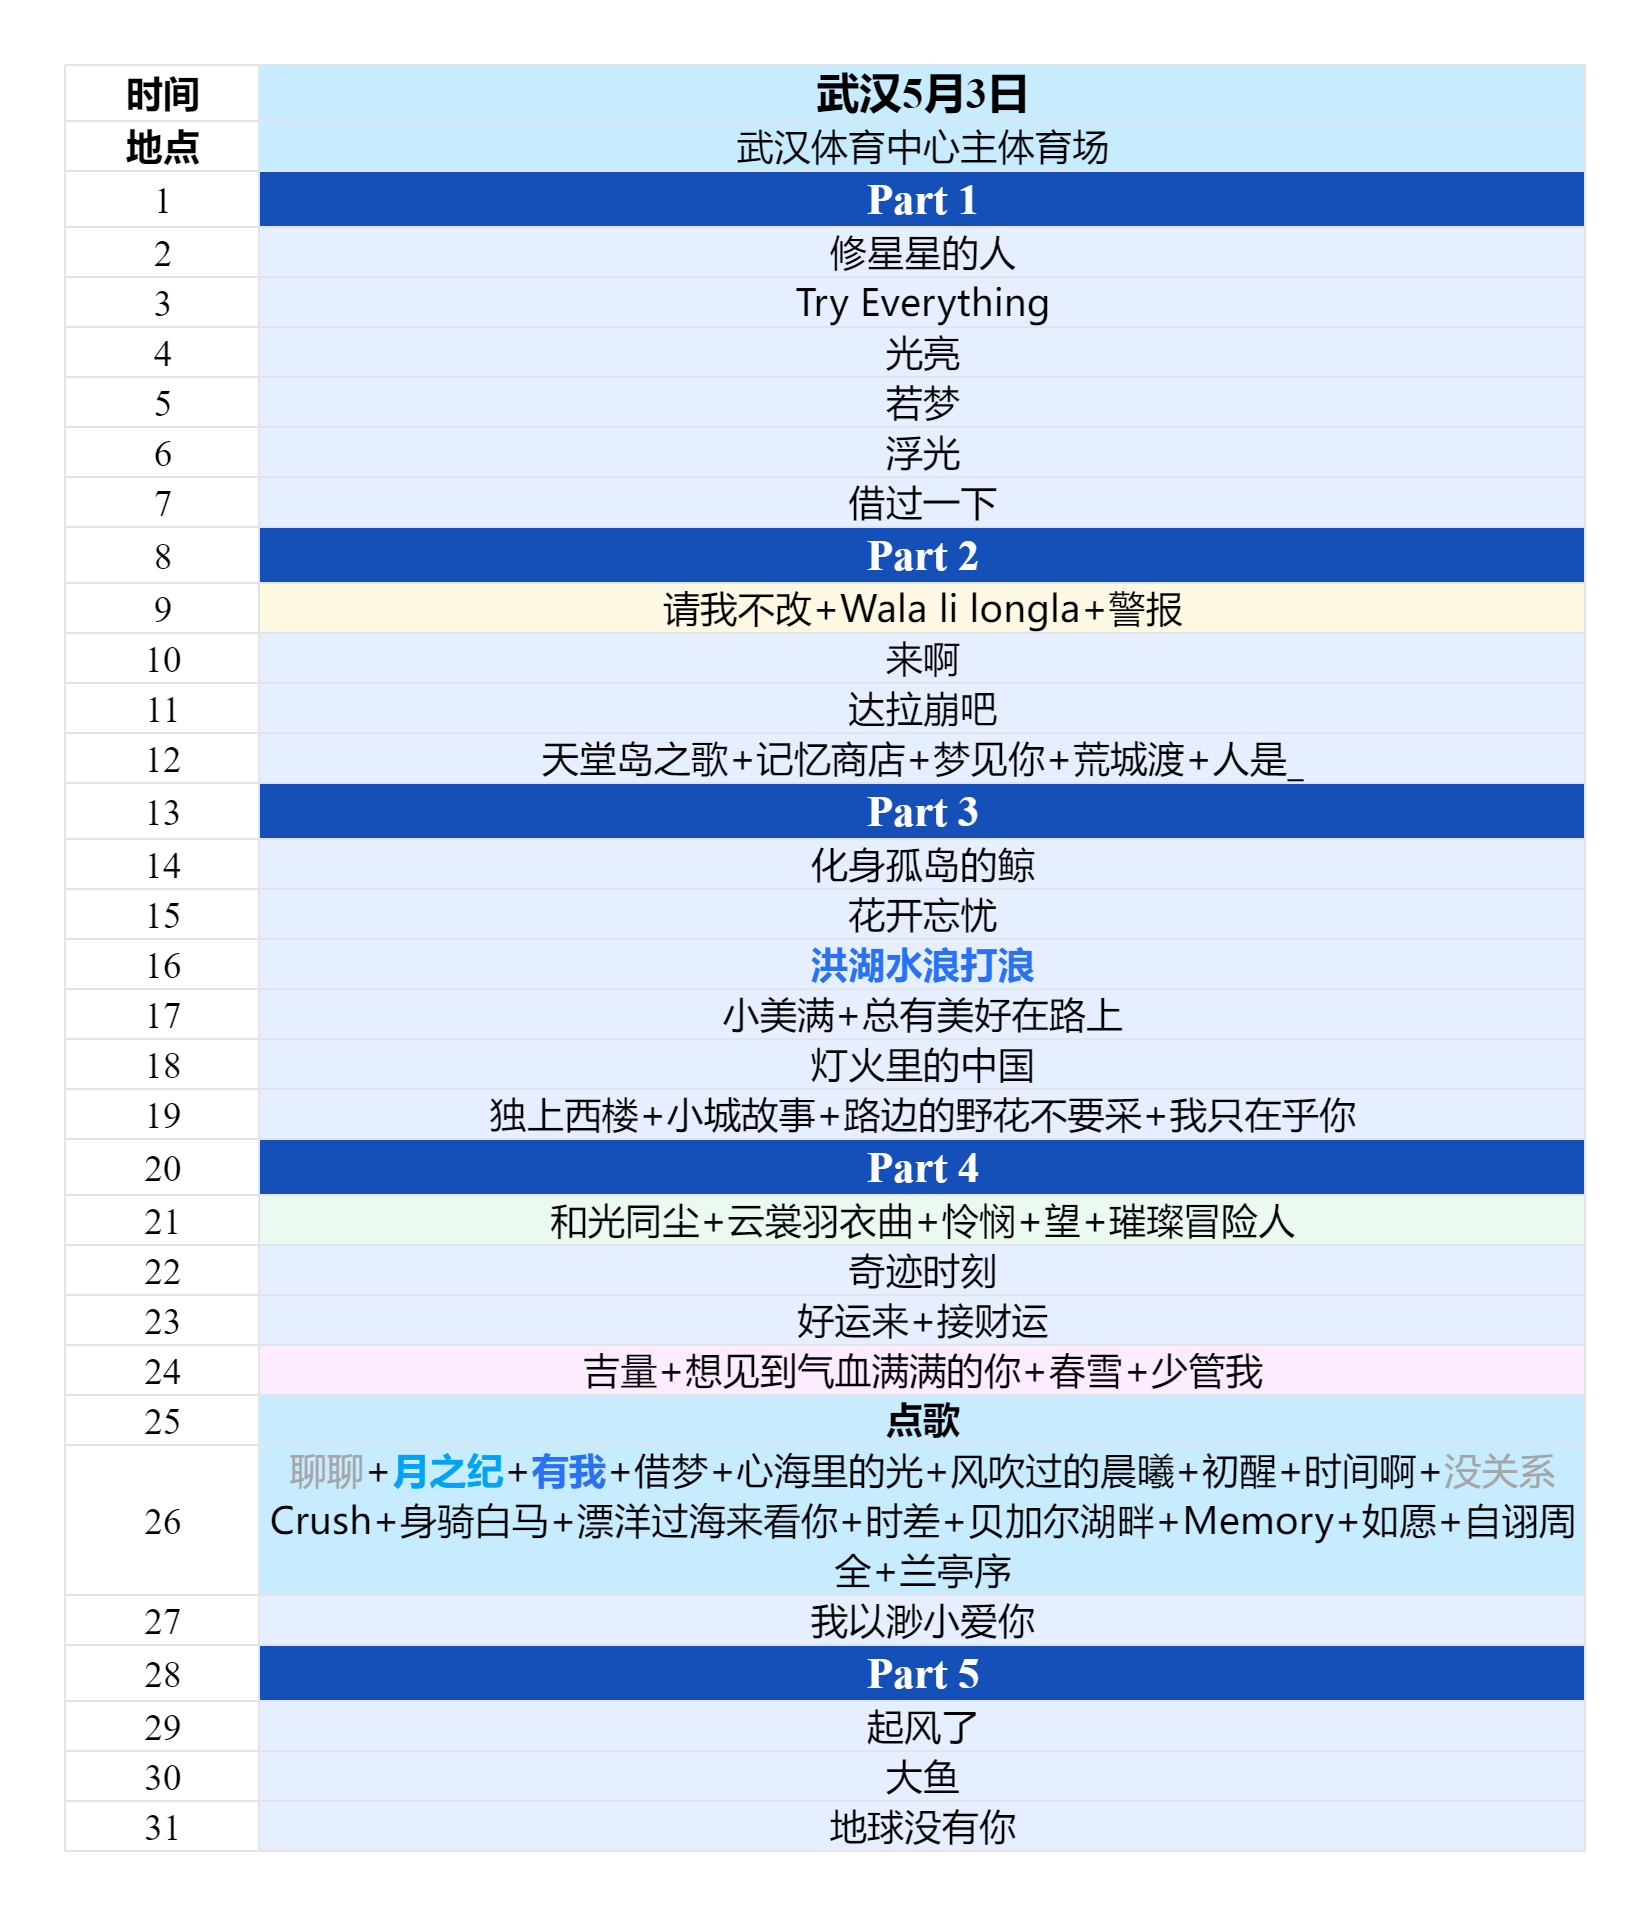
\includegraphics[width=280pt]{img/playlists/WuHan-20260503} 

}

\caption{2026周深“深深的”巡回演唱会2026.05.03武汉场歌单}\label{fig:unnamed-chunk-12}
\end{figure}

\newpage

\section{Part1}\label{WuHan-20260503-part1}

\hyperref[opening-vcr]{🎥【\textbf{开场VCR}】}

\hyperref[xiu-xing-xing-de-ren]{🎵【\textbf{修星星的人}】}

\hyperref[try-everything]{🎵【\textbf{Try Everything}】}

\hyperref[silver-linings]{🎵【\textbf{光亮}】}

\hyperref[like-a-dream]{🎵【\textbf{若梦}】}

\hyperref[floating-light]{🎵【\textbf{浮光}】}

\hyperref[excuse-me]{🎵【\textbf{借过一下}】}

\section{Part2}\label{WuHan-20260503-part2}

\hyperref[robot-vcr]{🎥【\textbf{机器人VCR}】}

\hyperref[brave-heart]{🎵【\textbf{请我不改}】}

\hyperref[wala-li-longla]{🎵【\textbf{Wala li longla}】}

\hyperref[jing-bao]{🎵【\textbf{警报}】}

\hyperref[lai-a]{🎵【\textbf{来啊}】}

\hyperref[dalabengba]{🎵【\textbf{达拉崩吧}】}

\hyperref[haven-song]{🎵【\textbf{天堂岛之歌}】}

\hyperref[the-memory-store]{🎵【\textbf{记忆商店}】}

\hyperref[meng-jian-ni]{🎵【\textbf{梦见你}】}

\hyperref[huang-cheng-du]{🎵【\textbf{荒城渡}】}

\hyperref[Humans_are_]{🎵【\textbf{人是\_}】}

\section{Part3}\label{WuHan-20260503-part3}

\hyperref[music-animations-vcr]{🎥【\textbf{音乐动画VCR}】}

\hyperref[The-whale-who-became-an-island]{🎵【\textbf{化身孤岛的鲸}】}

\hyperref[Blossoms-that-forget-sorrow]{🎵【\textbf{花开忘忧}】}

\hyperref[hong-hu-shui-lang-da-lang]{🎵【\textbf{洪湖水浪打浪}】}

\hyperref[simple-bliss]{🎵【\textbf{小美满}】}

\hyperref[zong-you-mei-hao-zai-lu-shang]{🎵【\textbf{总有美好在路上}】}

\hyperref[deng-huo-li-de-zhong-guo]{🎵【\textbf{灯火里的中国}】}

🎵【\textbf{邓丽君组曲}】

\hyperref[du-shang-xi-lou]{🎵【\textbf{独上西楼}】}

\hyperref[xiao-cheng-gu-shi]{🎵【\textbf{小城故事}】}

\hyperref[donot-pick-the-roadside-flowers]{🎵【\textbf{路边的野花不要采}】}

\hyperref[I-only-care-about-you]{🎵【\textbf{我只在乎你}】}

\section{Part4}\label{WuHan-20260503-part4}

\hyperref[mask-vcr]{🎥【\textbf{面具VCR}】}

\hyperref[stay-with-light]{🎵【\textbf{和光同尘}】}

\hyperref[Song-of-the-cloud-dress]{🎵【\textbf{云裳羽衣曲}】}

\hyperref[lian-min]{🎵【\textbf{怜悯}】}

\hyperref[Expectation]{🎵【\textbf{望}】}

\hyperref[adventurers]{🎵【\textbf{璀璨冒险人}】}

\hyperref[miracle-moment]{🎵【\textbf{奇迹时刻}】}

\hyperref[good-fortune-comes]{🎵【\textbf{好运来}】}

\hyperref[jie-cai-yun]{🎵【\textbf{接财运}】}

\hyperref[ji-liang]{🎵【\textbf{吉量}】}

\hyperref[xiang-jian-dao-qi-xue-man-man-de-ni]{🎵【\textbf{想见到气血满满的你}】}

\hyperref[chun-xue]{🎵【\textbf{春雪}】}

\hyperref[watch-ur-manners]{🎵【\textbf{少管我}】}

【\textbf{点歌环节}】

\hyperref[you-wo]{🎵【\textbf{有我}】}

\hyperref[yue-zhi-ji]{🎵【\textbf{月之纪}】}

\hyperref[loving-you-in-my-humble-way]{🎵【\textbf{我以渺小爱你}】}

\section{Part5}\label{WuHan-20260503-part5}

\hyperref[exchange-diaries-vcr]{🎥【\textbf{交换日记VCR}】}

\hyperref[the-wind-rises]{🎵【\textbf{起风了}】}

\hyperref[big-fish]{🎵【\textbf{大鱼}】}

\hyperref[di-qiu-mei-you-ni]{🎵【\textbf{地球没有你}】}

\chapter{2026.05.16苏州场 (WIP)}\label{SuZhou-20260516}

\begin{quote}
\begin{flushright}------周深\end{flushright}
\end{quote}

\begin{figure}

{\centering 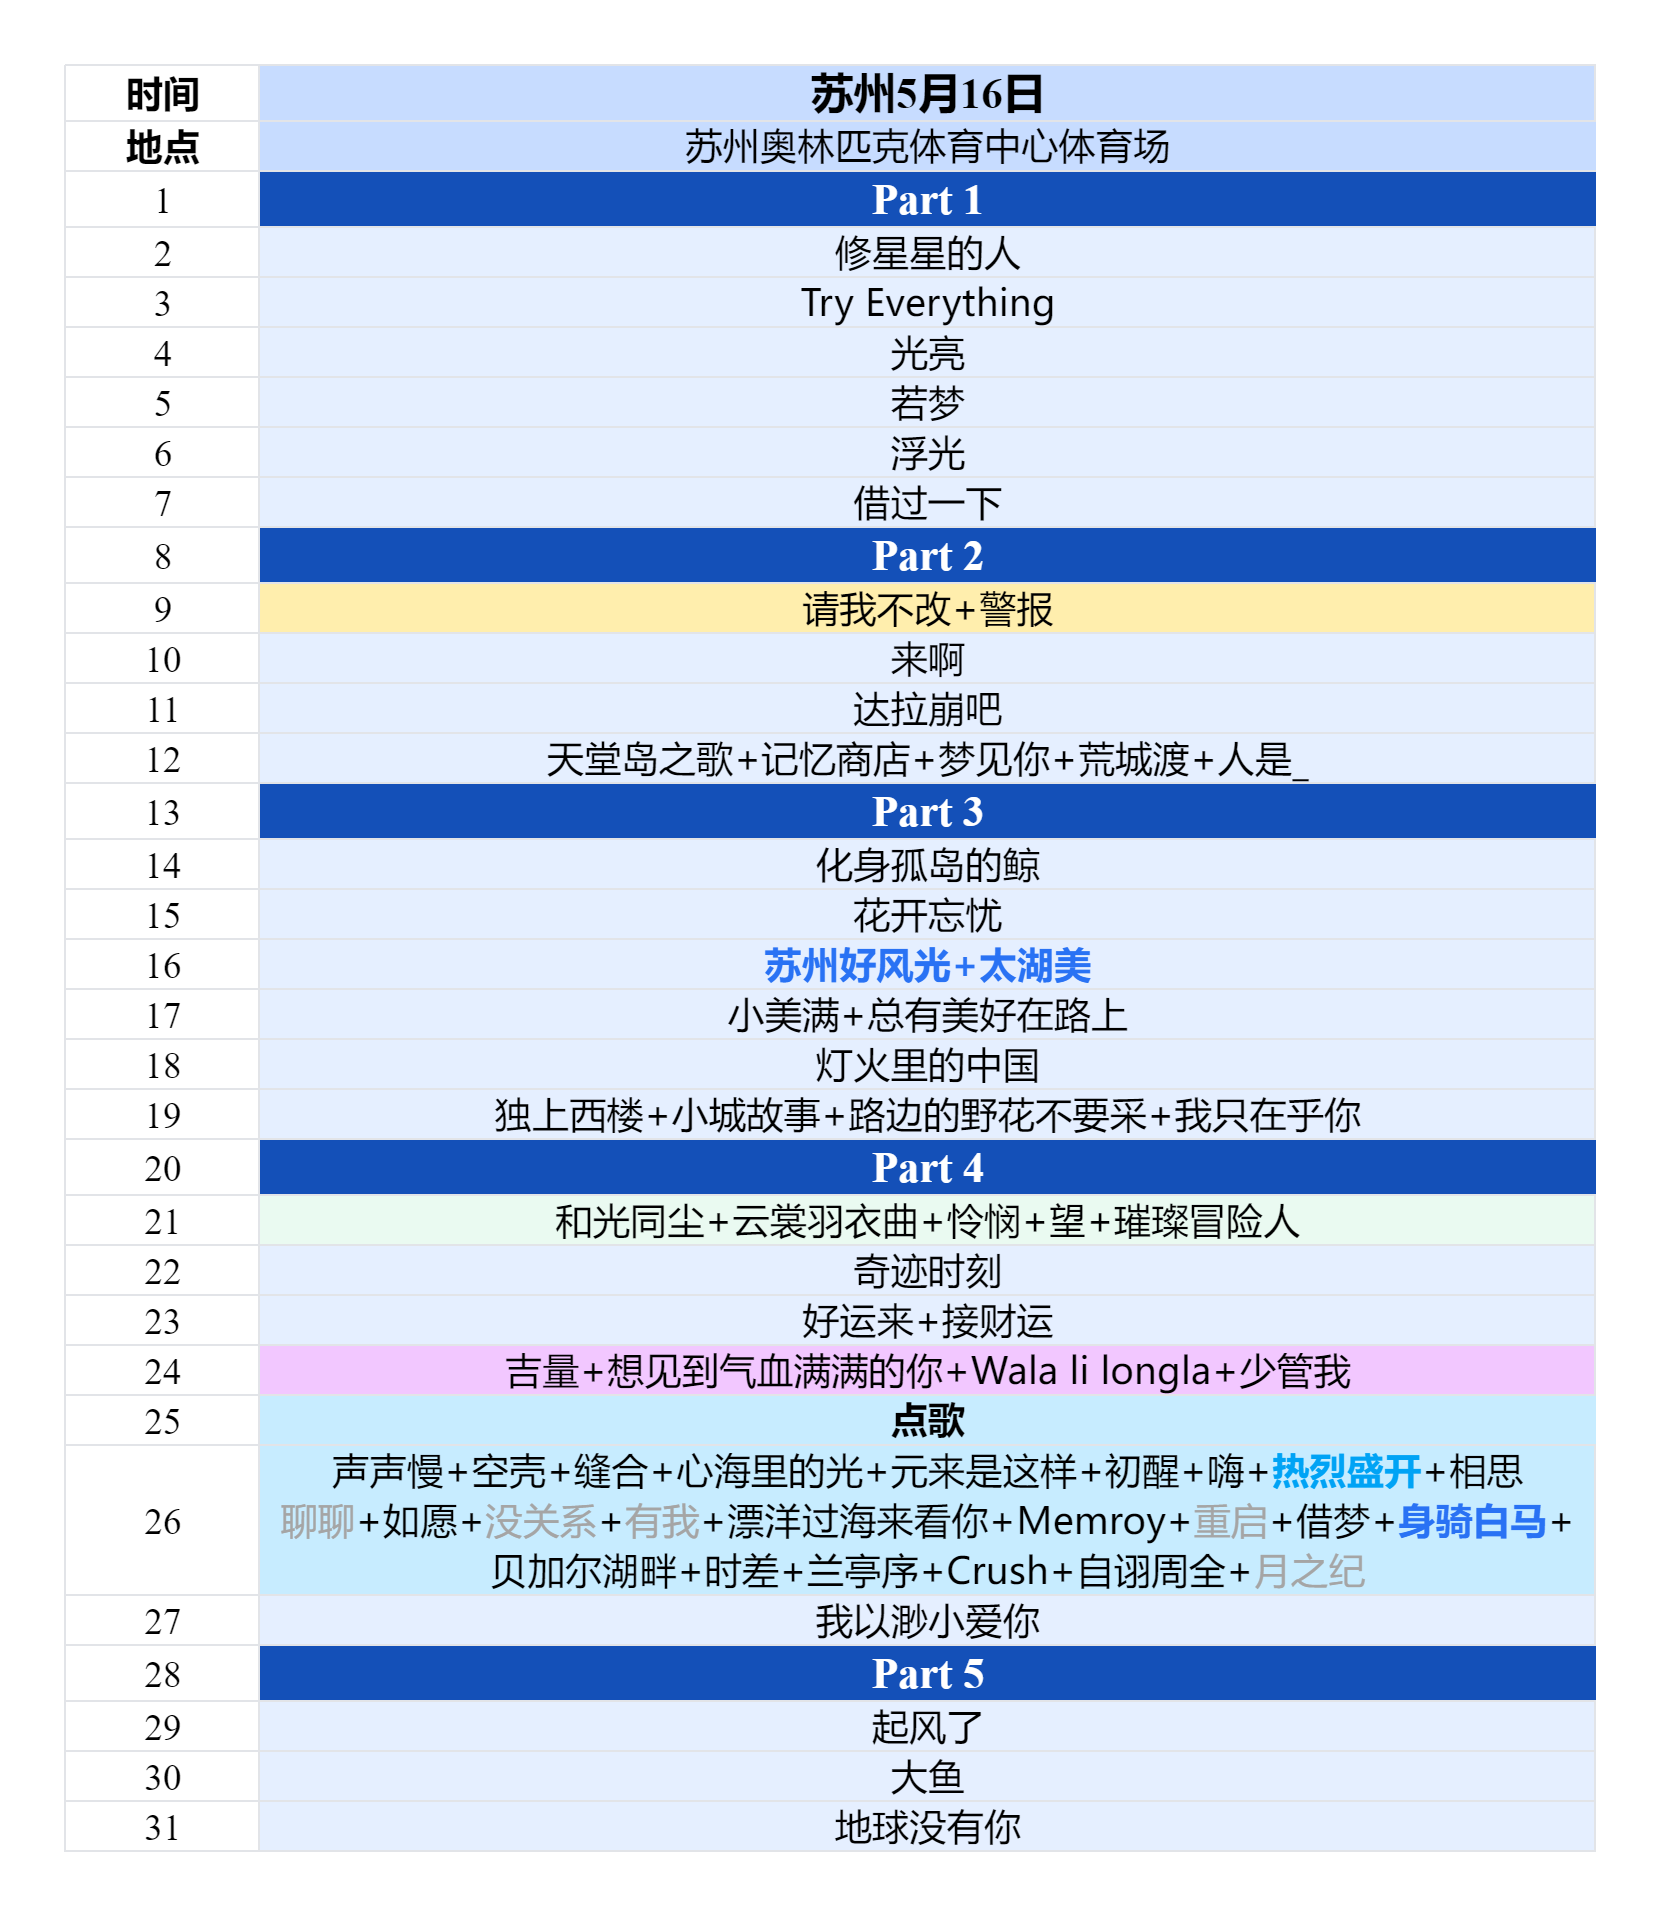
\includegraphics[width=280pt]{img/playlists/SuZhou-20260516} 

}

\caption{2026周深“深深的”巡回演唱会2026.05.16苏州场歌单}\label{fig:unnamed-chunk-14}
\end{figure}

\newpage

\section{Part1}\label{SuZhou-20260516-part1}

\hyperref[opening-vcr]{🎥【\textbf{开场VCR}】}

\hyperref[xiu-xing-xing-de-ren]{🎵【\textbf{修星星的人}】}

\hyperref[try-everything]{🎵【\textbf{Try Everything}】}

\hyperref[silver-linings]{🎵【\textbf{光亮}】}

\hyperref[like-a-dream]{🎵【\textbf{若梦}】}

\hyperref[floating-light]{🎵【\textbf{浮光}】}

\hyperref[excuse-me]{🎵【\textbf{借过一下}】}

\section{Part2}\label{SuZhou-20260516-part2}

\hyperref[robot-vcr]{🎥【\textbf{机器人VCR}】}

\hyperref[brave-heart]{🎵【\textbf{请我不改}】}

\hyperref[jing-bao]{🎵【\textbf{警报}】}

\hyperref[lai-a]{🎵【\textbf{来啊}】}

\hyperref[dalabengba]{🎵【\textbf{达拉崩吧}】}

\hyperref[haven-song]{🎵【\textbf{天堂岛之歌}】}

\hyperref[the-memory-store]{🎵【\textbf{记忆商店}】}

\hyperref[meng-jian-ni]{🎵【\textbf{梦见你}】}

\hyperref[huang-cheng-du]{🎵【\textbf{荒城渡}】}

\hyperref[Humans_are_]{🎵【\textbf{人是\_}】}

\section{Part3}\label{SuZhou-20260516-part3}

\hyperref[music-animations-vcr]{🎥【\textbf{音乐动画VCR}】}

\hyperref[The-whale-who-became-an-island]{🎵【\textbf{化身孤岛的鲸}】}

\hyperref[Blossoms-that-forget-sorrow]{🎵【\textbf{花开忘忧}】}

\hyperref[su-zhou-hao-feng-guang]{🎵【\textbf{苏州好风光}】}

\hyperref[tai-hu-mei]{🎵【\textbf{太湖美}】}

\hyperref[simple-bliss]{🎵【\textbf{小美满}】}

\hyperref[zong-you-mei-hao-zai-lu-shang]{🎵【\textbf{总有美好在路上}】}

\hyperref[deng-huo-li-de-zhong-guo]{🎵【\textbf{灯火里的中国}】}

🎵【\textbf{邓丽君组曲}】

\hyperref[du-shang-xi-lou]{🎵【\textbf{独上西楼}】}

\hyperref[xiao-cheng-gu-shi]{🎵【\textbf{小城故事}】}

\hyperref[donot-pick-the-roadside-flowers]{🎵【\textbf{路边的野花不要采}】}

\hyperref[I-only-care-about-you]{🎵【\textbf{我只在乎你}】}

\section{Part4}\label{SuZhou-20260516-part4}

\hyperref[mask-vcr]{🎥【\textbf{面具VCR}】}

\hyperref[stay-with-light]{🎵【\textbf{和光同尘}】}

\hyperref[Song-of-the-cloud-dress]{🎵【\textbf{云裳羽衣曲}】}

\hyperref[lian-min]{🎵【\textbf{怜悯}】}

\hyperref[Expectation]{🎵【\textbf{望}】}

\hyperref[adventurers]{🎵【\textbf{璀璨冒险人}】}

\hyperref[miracle-moment]{🎵【\textbf{奇迹时刻}】}

\hyperref[good-fortune-comes]{🎵【\textbf{好运来}】}

\hyperref[jie-cai-yun]{🎵【\textbf{接财运}】}

\hyperref[ji-liang]{🎵【\textbf{吉量}】}

\hyperref[xiang-jian-dao-qi-xue-man-man-de-ni]{🎵【\textbf{想见到气血满满的你}】}

\hyperref[wala-li-longla]{🎵【\textbf{Wala li longla}】}

\hyperref[watch-ur-manners]{🎵【\textbf{少管我}】}

【\textbf{点歌环节}】

\hyperref[shen-qi-bai-ma]{🎵【\textbf{身骑白马}】}

\hyperref[re-lie-sheng-kai]{🎵【\textbf{热烈盛开}】}

\hyperref[loving-you-in-my-humble-way]{🎵【\textbf{我以渺小爱你}】}

\section{Part5}\label{SuZhou-20260516-part5}

\hyperref[exchange-diaries-vcr]{🎥【\textbf{交换日记VCR}】}

\hyperref[the-wind-rises]{🎵【\textbf{起风了}】}

\hyperref[big-fish]{🎵【\textbf{大鱼}】}

\hyperref[di-qiu-mei-you-ni]{🎵【\textbf{地球没有你}】}

\chapter{2026.05.17苏州场 (WIP)}\label{SuZhou-20260517}

\begin{quote}
\begin{flushright}------周深\end{flushright}
\end{quote}

\begin{figure}

{\centering 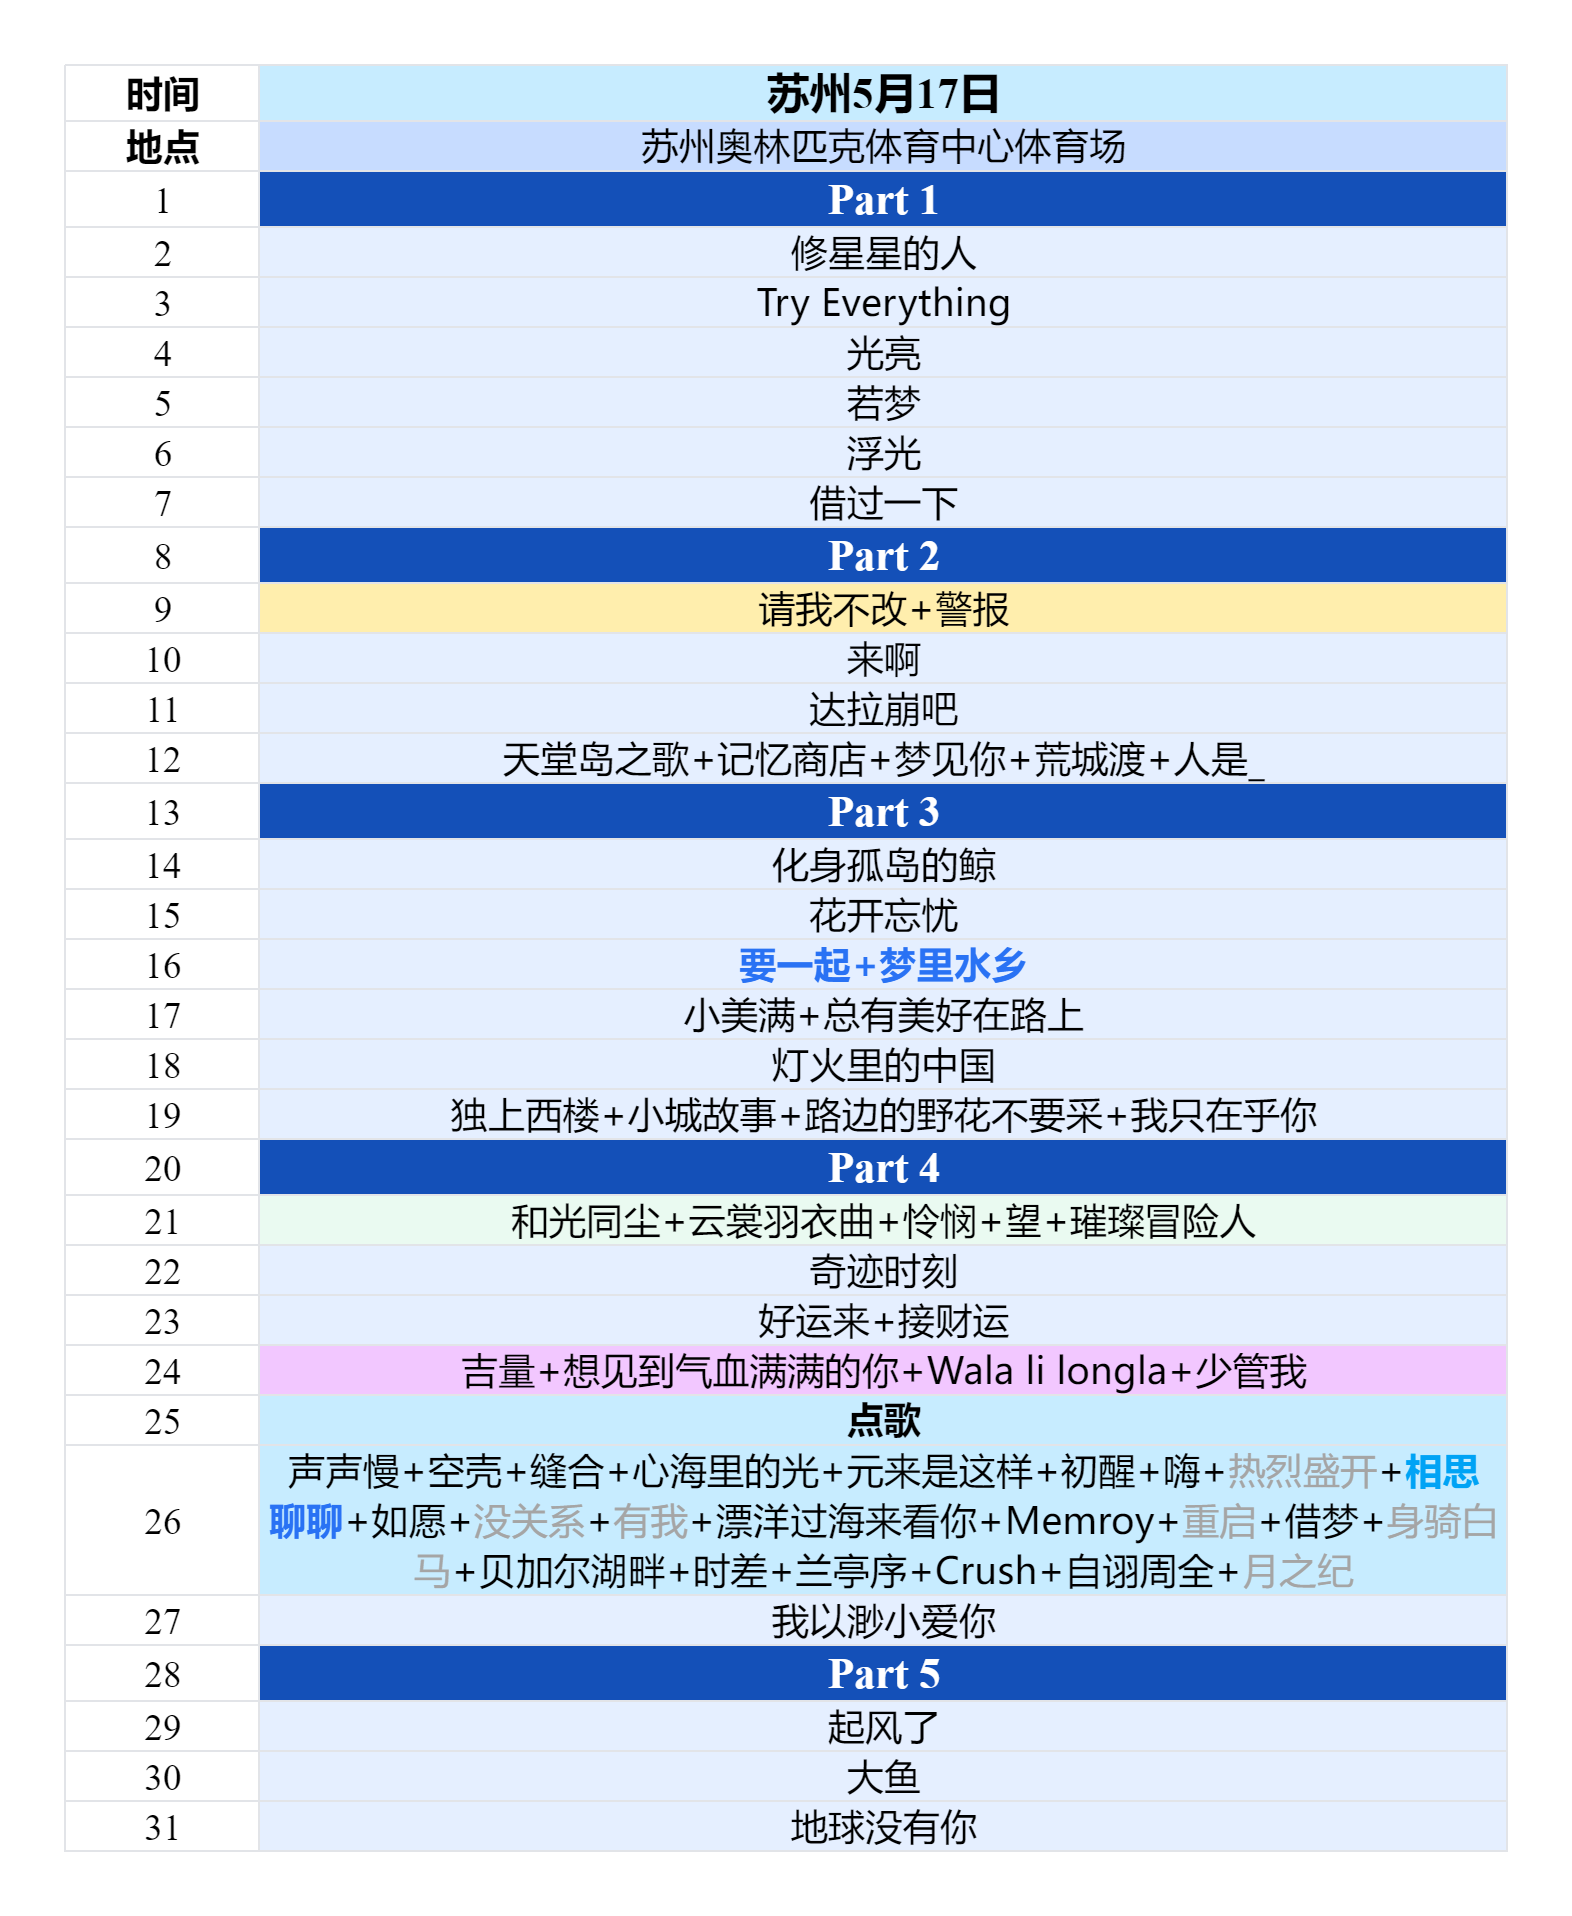
\includegraphics[width=280pt]{img/playlists/SuZhou-20260517} 

}

\caption{2026周深“深深的”巡回演唱会2026.05.17苏州场歌单}\label{fig:unnamed-chunk-16}
\end{figure}

\newpage

\section{Part1}\label{SuZhou-20260517-part1}

\hyperref[opening-vcr]{🎥【\textbf{开场VCR}】}

\hyperref[xiu-xing-xing-de-ren]{🎵【\textbf{修星星的人}】}

\hyperref[try-everything]{🎵【\textbf{Try Everything}】}

\hyperref[silver-linings]{🎵【\textbf{光亮}】}

\hyperref[like-a-dream]{🎵【\textbf{若梦}】}

\hyperref[floating-light]{🎵【\textbf{浮光}】}

\hyperref[excuse-me]{🎵【\textbf{借过一下}】}

\section{Part2}\label{SuZhou-20260517-part2}

\hyperref[robot-vcr]{🎥【\textbf{机器人VCR}】}

\hyperref[brave-heart]{🎵【\textbf{请我不改}】}

\hyperref[jing-bao]{🎵【\textbf{警报}】}

\hyperref[lai-a]{🎵【\textbf{来啊}】}

\hyperref[dalabengba]{🎵【\textbf{达拉崩吧}】}

\hyperref[haven-song]{🎵【\textbf{天堂岛之歌}】}

\hyperref[the-memory-store]{🎵【\textbf{记忆商店}】}

\hyperref[meng-jian-ni]{🎵【\textbf{梦见你}】}

\hyperref[huang-cheng-du]{🎵【\textbf{荒城渡}】}

\hyperref[Humans_are_]{🎵【\textbf{人是\_}】}

\section{Part3}\label{SuZhou-20260517-part3}

\hyperref[music-animations-vcr]{🎥【\textbf{音乐动画VCR}】}

\hyperref[The-whale-who-became-an-island]{🎵【\textbf{化身孤岛的鲸}】}

\hyperref[Blossoms-that-forget-sorrow]{🎵【\textbf{花开忘忧}】}

\hyperref[yao-yi-qi]{🎵【\textbf{要一起}】}

\hyperref[meng-li-shui-xiang]{🎵【\textbf{梦里水乡}】}

\hyperref[simple-bliss]{🎵【\textbf{小美满}】}

\hyperref[zong-you-mei-hao-zai-lu-shang]{🎵【\textbf{总有美好在路上}】}

\hyperref[deng-huo-li-de-zhong-guo]{🎵【\textbf{灯火里的中国}】}

🎵【\textbf{邓丽君组曲}】

\hyperref[du-shang-xi-lou]{🎵【\textbf{独上西楼}】}

\hyperref[xiao-cheng-gu-shi]{🎵【\textbf{小城故事}】}

\hyperref[donot-pick-the-roadside-flowers]{🎵【\textbf{路边的野花不要采}】}

\hyperref[I-only-care-about-you]{🎵【\textbf{我只在乎你}】}

\section{Part4}\label{SuZhou-20260517-part4}

\hyperref[mask-vcr]{🎥【\textbf{面具VCR}】}

\hyperref[stay-with-light]{🎵【\textbf{和光同尘}】}

\hyperref[Song-of-the-cloud-dress]{🎵【\textbf{云裳羽衣曲}】}

\hyperref[lian-min]{🎵【\textbf{怜悯}】}

\hyperref[Expectation]{🎵【\textbf{望}】}

\hyperref[adventurers]{🎵【\textbf{璀璨冒险人}】}

\hyperref[miracle-moment]{🎵【\textbf{奇迹时刻}】}

\hyperref[good-fortune-comes]{🎵【\textbf{好运来}】}

\hyperref[jie-cai-yun]{🎵【\textbf{接财运}】}

\hyperref[ji-liang]{🎵【\textbf{吉量}】}

\hyperref[xiang-jian-dao-qi-xue-man-man-de-ni]{🎵【\textbf{想见到气血满满的你}】}

\hyperref[wala-li-longla]{🎵【\textbf{Wala li longla}】}

\hyperref[watch-ur-manners]{🎵【\textbf{少管我}】}

【\textbf{点歌环节}】

\hyperref[liao-liao]{🎵【\textbf{聊聊}】}

\hyperref[xiang-si]{🎵【\textbf{相思}】}

\hyperref[loving-you-in-my-humble-way]{🎵【\textbf{我以渺小爱你}】}

\section{Part5}\label{SuZhou-20260517-part5}

\hyperref[exchange-diaries-vcr]{🎥【\textbf{交换日记VCR}】}

\hyperref[the-wind-rises]{🎵【\textbf{起风了}】}

\hyperref[big-fish]{🎵【\textbf{大鱼}】}

\hyperref[di-qiu-mei-you-ni]{🎵【\textbf{地球没有你}】}

\chapter{2026.05.30重庆场 (WIP)}\label{ChongQing-20260530}

\begin{quote}
\begin{flushright}------周深\end{flushright}
\end{quote}

\begin{figure}

{\centering 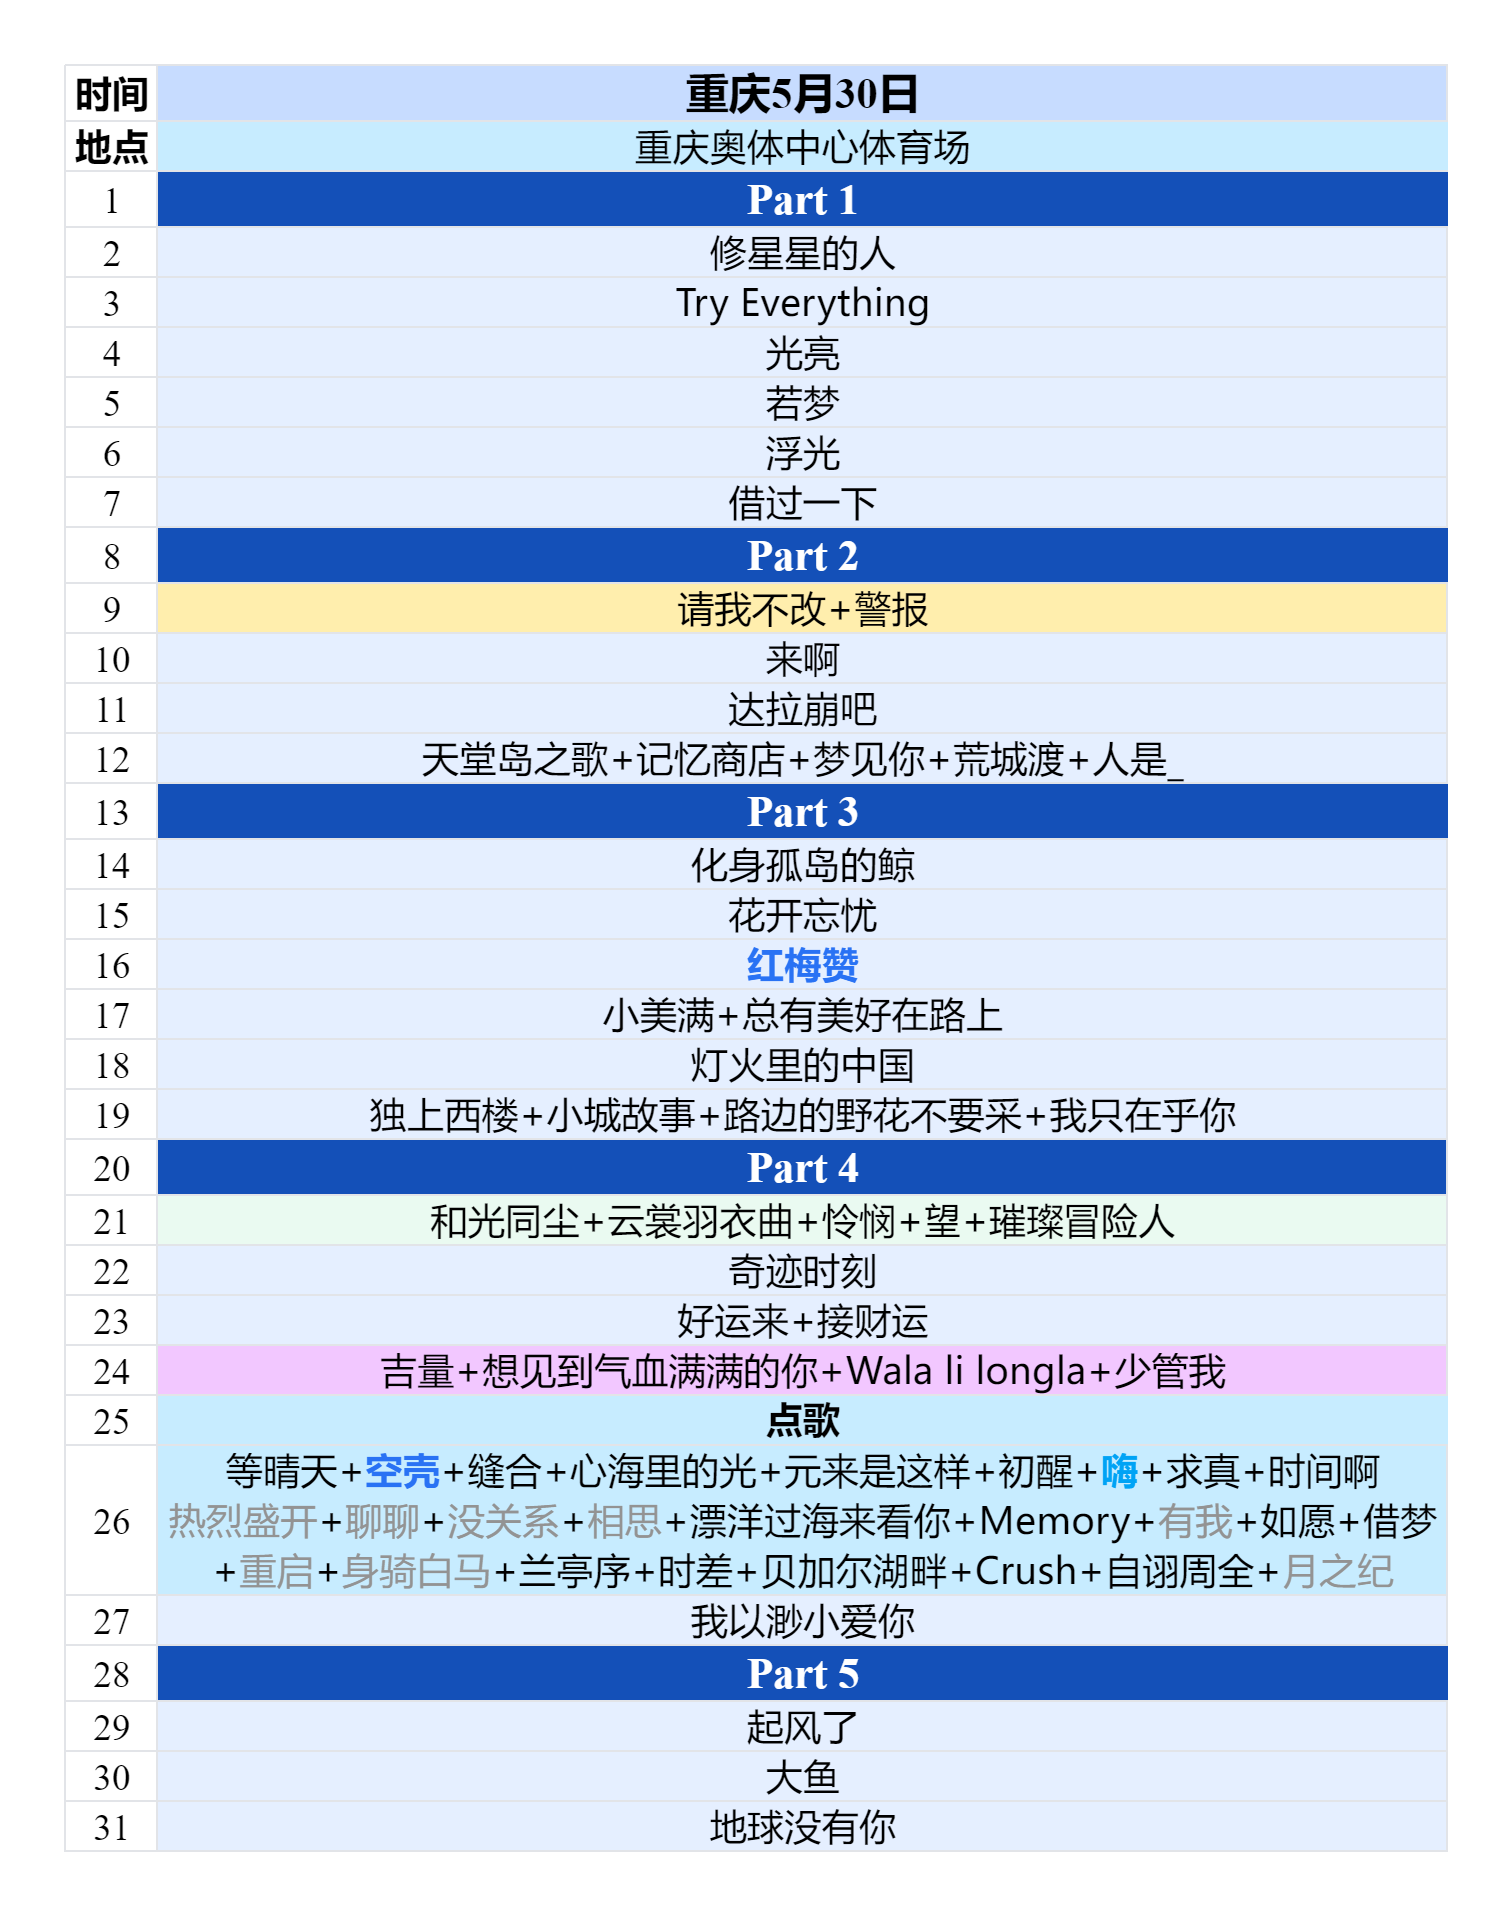
\includegraphics[width=280pt]{img/playlists/ChongQing-20260530} 

}

\caption{2026周深“深深的”巡回演唱会2026.05.30重庆场歌单}\label{fig:unnamed-chunk-18}
\end{figure}

\newpage

\section{Part1}\label{ChongQing-20260530-part1}

\hyperref[opening-vcr]{🎥【\textbf{开场VCR}】}

\hyperref[xiu-xing-xing-de-ren]{🎵【\textbf{修星星的人}】}

\hyperref[try-everything]{🎵【\textbf{Try Everything}】}

\hyperref[silver-linings]{🎵【\textbf{光亮}】}

\hyperref[like-a-dream]{🎵【\textbf{若梦}】}

\hyperref[floating-light]{🎵【\textbf{浮光}】}

\hyperref[excuse-me]{🎵【\textbf{借过一下}】}

\section{Part2}\label{ChongQing-20260530-part2}

\hyperref[robot-vcr]{🎥【\textbf{机器人VCR}】}

\hyperref[brave-heart]{🎵【\textbf{请我不改}】}

\hyperref[jing-bao]{🎵【\textbf{警报}】}

\hyperref[lai-a]{🎵【\textbf{来啊}】}

\hyperref[dalabengba]{🎵【\textbf{达拉崩吧}】}

\hyperref[haven-song]{🎵【\textbf{天堂岛之歌}】}

\hyperref[the-memory-store]{🎵【\textbf{记忆商店}】}

\hyperref[meng-jian-ni]{🎵【\textbf{梦见你}】}

\hyperref[huang-cheng-du]{🎵【\textbf{荒城渡}】}

\hyperref[Humans_are_]{🎵【\textbf{人是\_}】}

\section{Part3}\label{ChongQing-20260530-part3}

\hyperref[music-animations-vcr]{🎥【\textbf{音乐动画VCR}】}

\hyperref[The-whale-who-became-an-island]{🎵【\textbf{化身孤岛的鲸}】}

\hyperref[Blossoms-that-forget-sorrow]{🎵【\textbf{花开忘忧}】}

\hyperref[hong-mei-zan]{🎵【\textbf{红梅赞}】}

\hyperref[simple-bliss]{🎵【\textbf{小美满}】}

\hyperref[zong-you-mei-hao-zai-lu-shang]{🎵【\textbf{总有美好在路上}】}

\hyperref[deng-huo-li-de-zhong-guo]{🎵【\textbf{灯火里的中国}】}

🎵【\textbf{邓丽君组曲}】

\hyperref[du-shang-xi-lou]{🎵【\textbf{独上西楼}】}

\hyperref[xiao-cheng-gu-shi]{🎵【\textbf{小城故事}】}

\hyperref[donot-pick-the-roadside-flowers]{🎵【\textbf{路边的野花不要采}】}

\hyperref[I-only-care-about-you]{🎵【\textbf{我只在乎你}】}

\section{Part4}\label{ChongQing-20260530-part4}

\hyperref[mask-vcr]{🎥【\textbf{面具VCR}】}

\hyperref[stay-with-light]{🎵【\textbf{和光同尘}】}

\hyperref[Song-of-the-cloud-dress]{🎵【\textbf{云裳羽衣曲}】}

\hyperref[lian-min]{🎵【\textbf{怜悯}】}

\hyperref[Expectation]{🎵【\textbf{望}】}

\hyperref[adventurers]{🎵【\textbf{璀璨冒险人}】}

\hyperref[miracle-moment]{🎵【\textbf{奇迹时刻}】}

\hyperref[good-fortune-comes]{🎵【\textbf{好运来}】}

\hyperref[jie-cai-yun]{🎵【\textbf{接财运}】}

\hyperref[ji-liang]{🎵【\textbf{吉量}】}

\hyperref[xiang-jian-dao-qi-xue-man-man-de-ni]{🎵【\textbf{想见到气血满满的你}】}

\hyperref[wala-li-longla]{🎵【\textbf{Wala li longla}】}

\hyperref[watch-ur-manners]{🎵【\textbf{少管我}】}

【\textbf{点歌环节}】

\hyperref[kong-ke]{🎵【\textbf{空壳}】}

\hyperref[say-hi]{🎵【\textbf{嗨}】}

\hyperref[loving-you-in-my-humble-way]{🎵【\textbf{我以渺小爱你}】}

\section{Part5}\label{ChongQing-20260530-part5}

\hyperref[exchange-diaries-vcr]{🎥【\textbf{交换日记VCR}】}

\hyperref[the-wind-rises]{🎵【\textbf{起风了}】}

\hyperref[big-fish]{🎵【\textbf{大鱼}】}

\hyperref[di-qiu-mei-you-ni]{🎵【\textbf{地球没有你}】}

\chapter{2026.05.31重庆场 (WIP)}\label{ChongQing-20260531}

\begin{quote}
\begin{flushright}------周深\end{flushright}
\end{quote}

\begin{figure}

{\centering 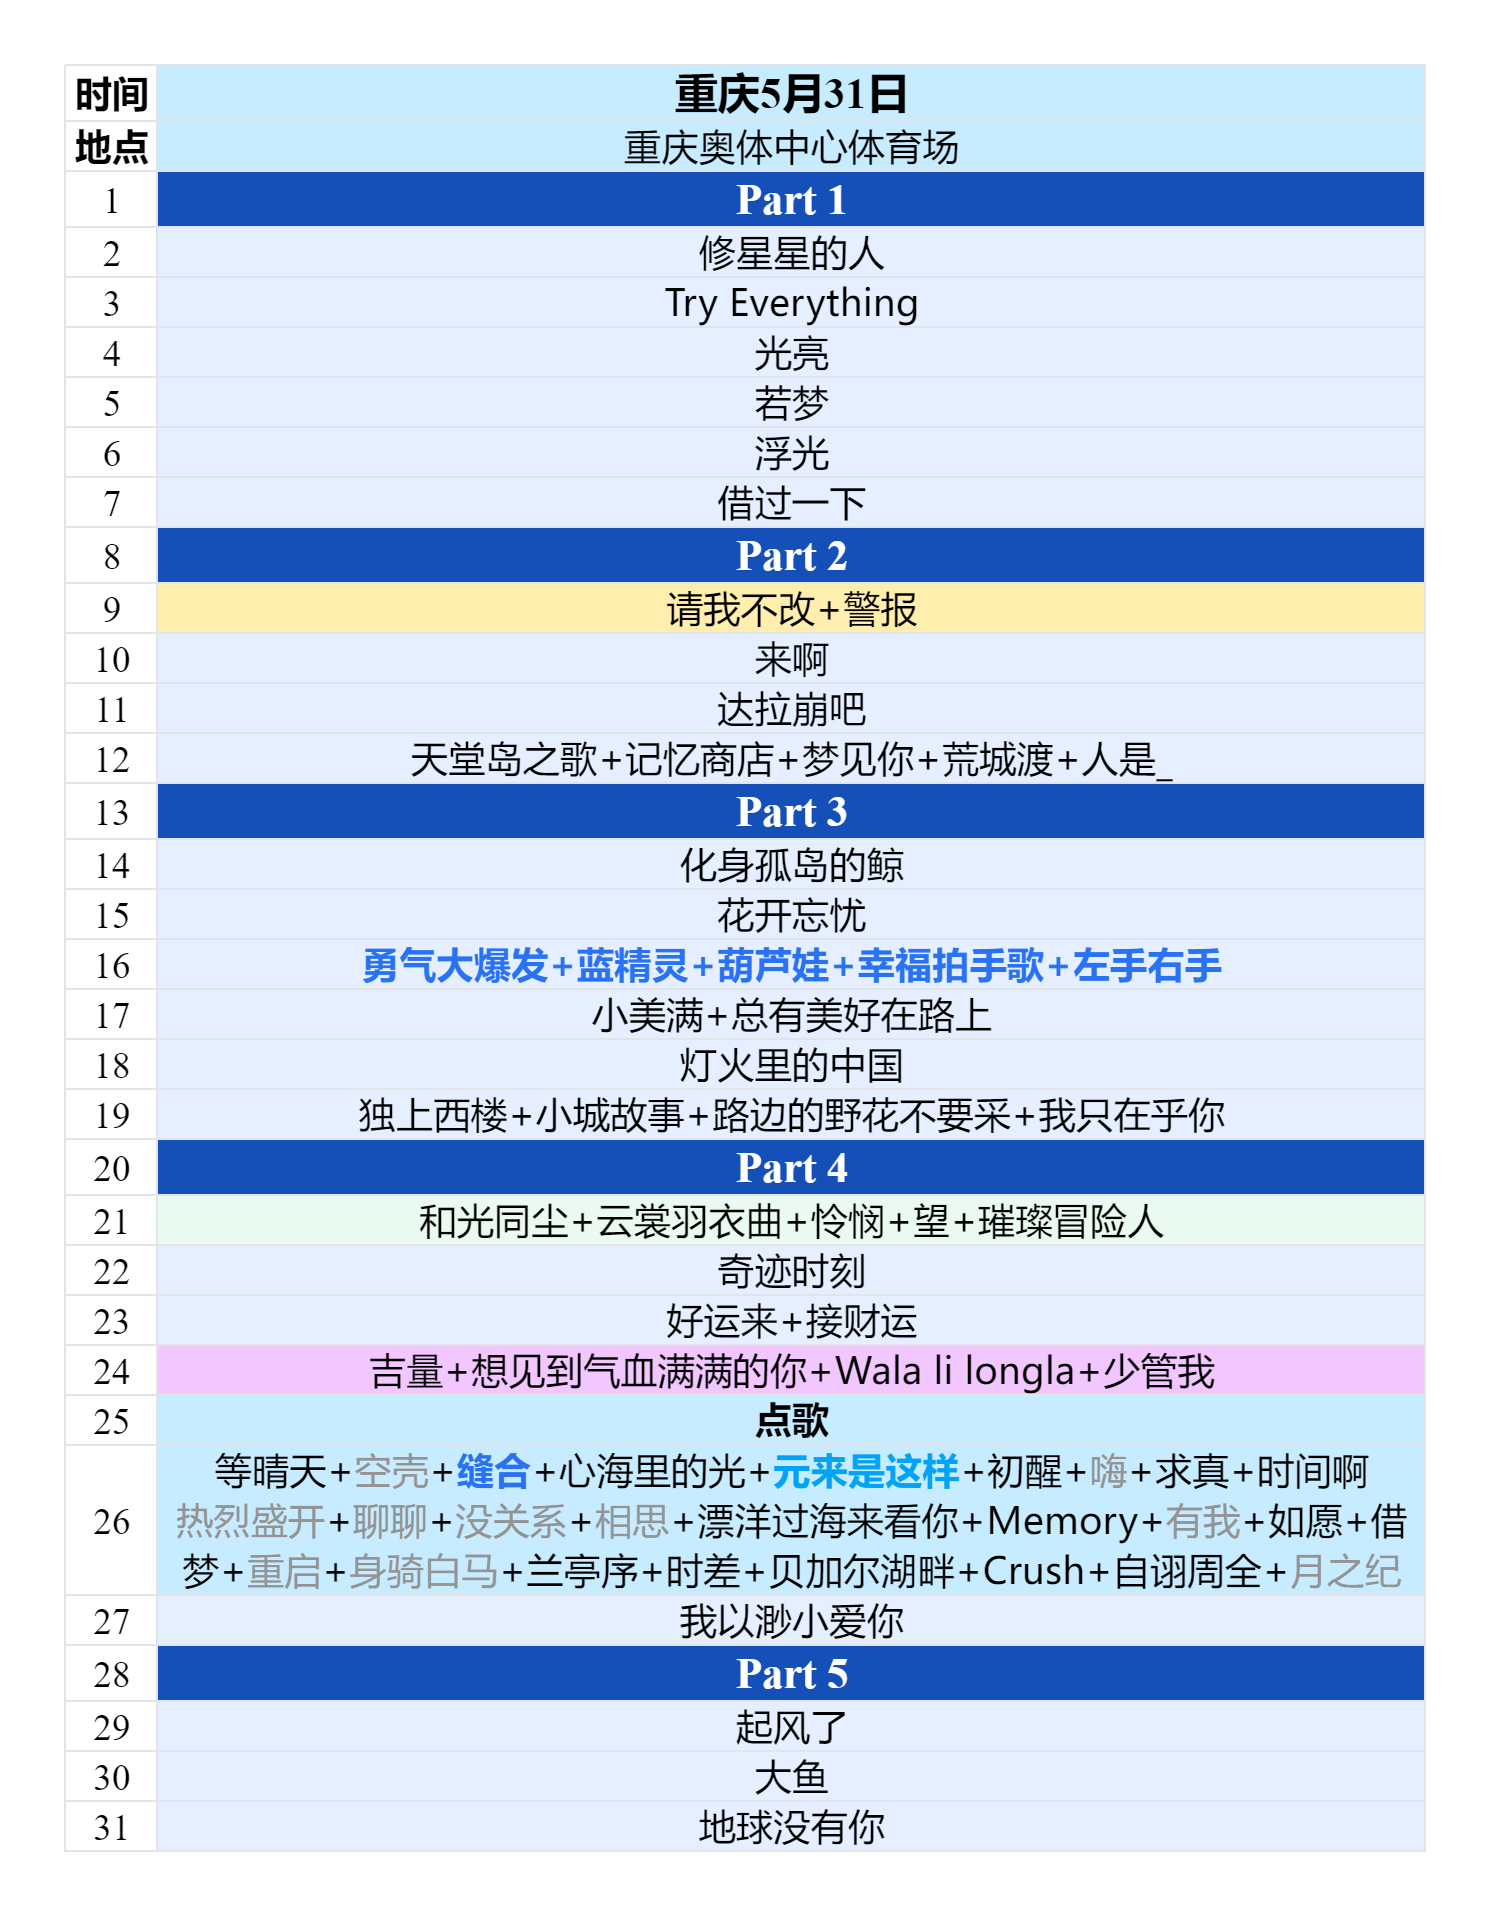
\includegraphics[width=280pt]{img/playlists/ChongQing-20260531} 

}

\caption{2026周深“深深的”巡回演唱会2026.05.31重庆场歌单}\label{fig:unnamed-chunk-20}
\end{figure}

\newpage

\section{Part1}\label{ChongQing-20260531-part1}

\hyperref[opening-vcr]{🎥【\textbf{开场VCR}】}

\hyperref[xiu-xing-xing-de-ren]{🎵【\textbf{修星星的人}】}

\hyperref[try-everything]{🎵【\textbf{Try Everything}】}

\hyperref[silver-linings]{🎵【\textbf{光亮}】}

\hyperref[like-a-dream]{🎵【\textbf{若梦}】}

\hyperref[floating-light]{🎵【\textbf{浮光}】}

\hyperref[excuse-me]{🎵【\textbf{借过一下}】}

\section{Part2}\label{ChongQing-20260531-part2}

\hyperref[robot-vcr]{🎥【\textbf{机器人VCR}】}

\hyperref[brave-heart]{🎵【\textbf{请我不改}】}

\hyperref[jing-bao]{🎵【\textbf{警报}】}

\hyperref[lai-a]{🎵【\textbf{来啊}】}

\hyperref[dalabengba]{🎵【\textbf{达拉崩吧}】}

\hyperref[haven-song]{🎵【\textbf{天堂岛之歌}】}

\hyperref[the-memory-store]{🎵【\textbf{记忆商店}】}

\hyperref[meng-jian-ni]{🎵【\textbf{梦见你}】}

\hyperref[huang-cheng-du]{🎵【\textbf{荒城渡}】}

\hyperref[Humans_are_]{🎵【\textbf{人是\_}】}

\section{Part3}\label{ChongQing-20260531-part3}

\hyperref[music-animations-vcr]{🎥【\textbf{音乐动画VCR}】}

\hyperref[The-whale-who-became-an-island]{🎵【\textbf{化身孤岛的鲸}】}

\hyperref[Blossoms-that-forget-sorrow]{🎵【\textbf{花开忘忧}】}

\hyperref[yong-qi-da-bao-fa]{🎵【\textbf{勇气大爆发}】}

\hyperref[lan-jing-ling]{🎵【\textbf{蓝精灵}】}

\hyperref[hu-lu-wa]{🎵【\textbf{葫芦娃}】}

\hyperref[xing-fu-pai-shou-ge]{🎵【\textbf{幸福拍手歌}】}

\hyperref[zuo-shou-you-shou]{🎵【\textbf{左手右手}】}

\hyperref[simple-bliss]{🎵【\textbf{小美满}】}

\hyperref[zong-you-mei-hao-zai-lu-shang]{🎵【\textbf{总有美好在路上}】}

\hyperref[deng-huo-li-de-zhong-guo]{🎵【\textbf{灯火里的中国}】}

🎵【\textbf{邓丽君组曲}】

\hyperref[du-shang-xi-lou]{🎵【\textbf{独上西楼}】}

\hyperref[xiao-cheng-gu-shi]{🎵【\textbf{小城故事}】}

\hyperref[donot-pick-the-roadside-flowers]{🎵【\textbf{路边的野花不要采}】}

\hyperref[I-only-care-about-you]{🎵【\textbf{我只在乎你}】}

\section{Part4}\label{ChongQing-20260531-part4}

\hyperref[mask-vcr]{🎥【\textbf{面具VCR}】}

\hyperref[stay-with-light]{🎵【\textbf{和光同尘}】}

\hyperref[Song-of-the-cloud-dress]{🎵【\textbf{云裳羽衣曲}】}

\hyperref[lian-min]{🎵【\textbf{怜悯}】}

\hyperref[Expectation]{🎵【\textbf{望}】}

\hyperref[adventurers]{🎵【\textbf{璀璨冒险人}】}

\hyperref[miracle-moment]{🎵【\textbf{奇迹时刻}】}

\hyperref[good-fortune-comes]{🎵【\textbf{好运来}】}

\hyperref[jie-cai-yun]{🎵【\textbf{接财运}】}

\hyperref[ji-liang]{🎵【\textbf{吉量}】}

\hyperref[xiang-jian-dao-qi-xue-man-man-de-ni]{🎵【\textbf{想见到气血满满的你}】}

\hyperref[wala-li-longla]{🎵【\textbf{Wala li longla}】}

\hyperref[watch-ur-manners]{🎵【\textbf{少管我}】}

【\textbf{点歌环节}】

\hyperref[feng-he]{🎵【\textbf{缝合}】}

\hyperref[yuan-lai-shi-zhe-yang]{🎵【\textbf{元来是这样}】}

\hyperref[loving-you-in-my-humble-way]{🎵【\textbf{我以渺小爱你}】}

\section{Part5}\label{ChongQing-20260531-part5}

\hyperref[exchange-diaries-vcr]{🎥【\textbf{交换日记VCR}】}

\hyperref[the-wind-rises]{🎵【\textbf{起风了}】}

\hyperref[big-fish]{🎵【\textbf{大鱼}】}

\hyperref[di-qiu-mei-you-ni]{🎵【\textbf{地球没有你}】}

\chapter{2026.06.27郑州场 (WIP)}\label{ZhengZhou-20260627}

\begin{quote}
\begin{flushright}------周深\end{flushright}
\end{quote}

\begin{figure}

{\centering 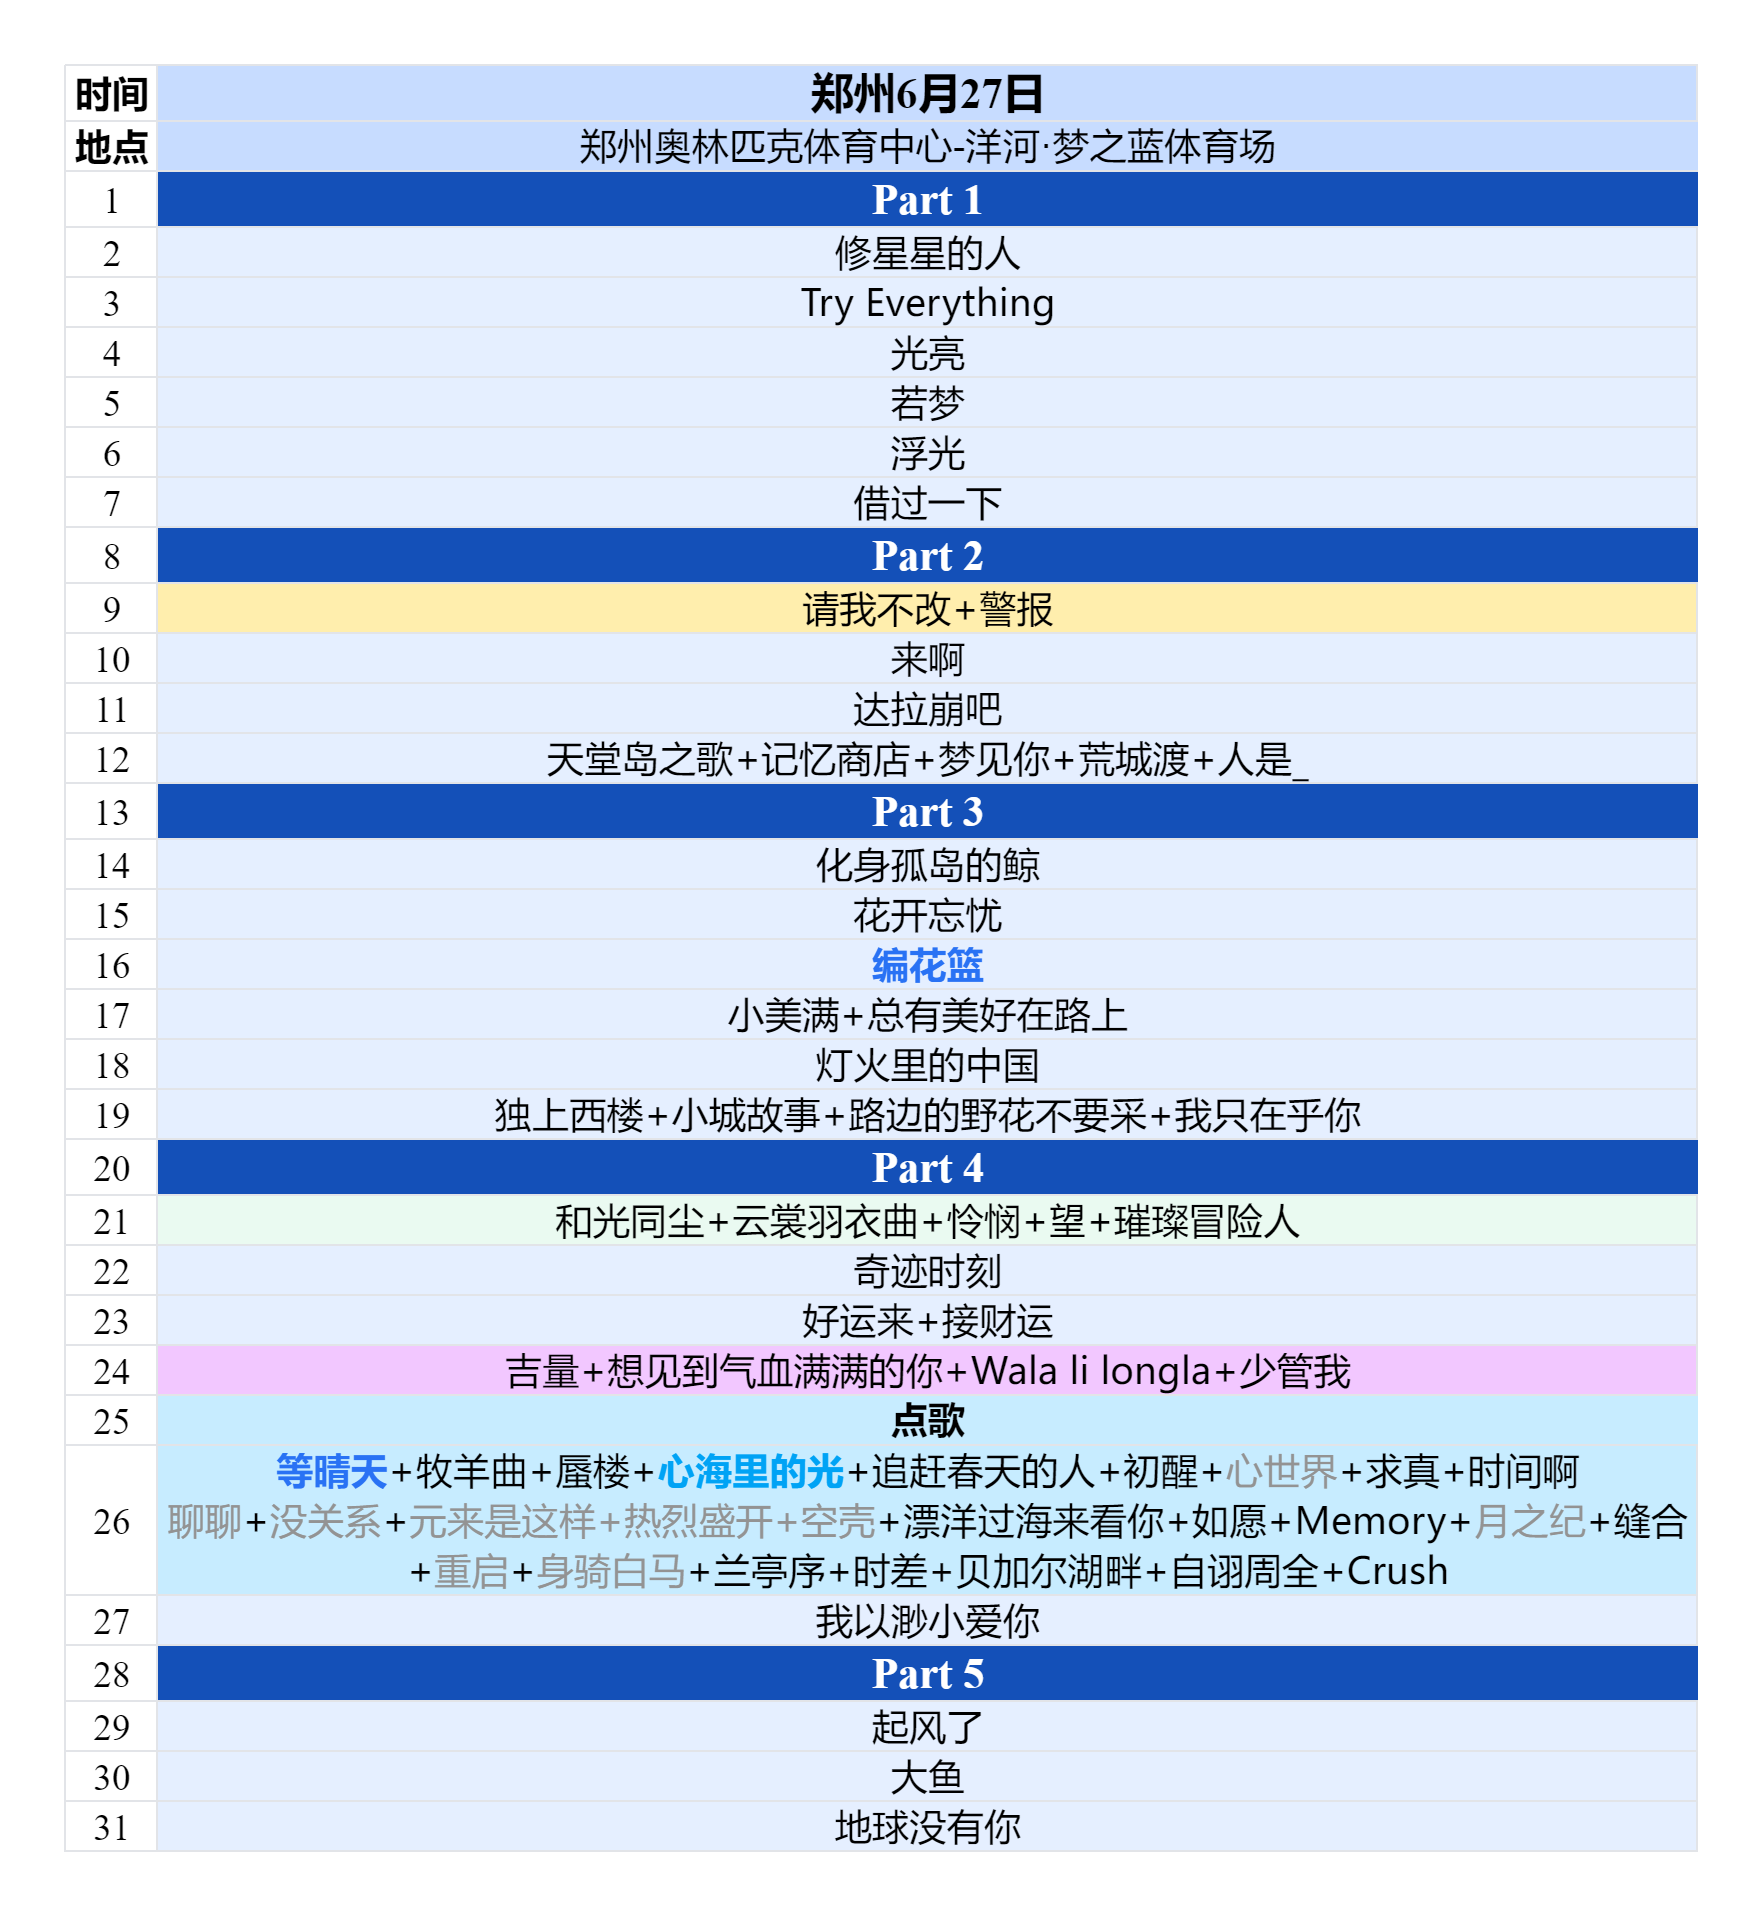
\includegraphics[width=280pt]{img/playlists/ZhengZhou-20260627} 

}

\caption{2026周深“深深的”巡回演唱会2026.06.27郑州场歌单}\label{fig:unnamed-chunk-22}
\end{figure}

\newpage

\section{Part1}\label{ZhengZhou-20260627-part1}

\hyperref[opening-vcr]{🎥【\textbf{开场VCR}】}

\hyperref[xiu-xing-xing-de-ren]{🎵【\textbf{修星星的人}】}

\hyperref[try-everything]{🎵【\textbf{Try Everything}】}

\hyperref[silver-linings]{🎵【\textbf{光亮}】}

\hyperref[like-a-dream]{🎵【\textbf{若梦}】}

\hyperref[floating-light]{🎵【\textbf{浮光}】}

\hyperref[excuse-me]{🎵【\textbf{借过一下}】}

\section{Part2}\label{ZhengZhou-20260627-part2}

\hyperref[robot-vcr]{🎥【\textbf{机器人VCR}】}

\hyperref[brave-heart]{🎵【\textbf{请我不改}】}

\hyperref[jing-bao]{🎵【\textbf{警报}】}

\hyperref[lai-a]{🎵【\textbf{来啊}】}

\hyperref[dalabengba]{🎵【\textbf{达拉崩吧}】}

\hyperref[haven-song]{🎵【\textbf{天堂岛之歌}】}

\hyperref[the-memory-store]{🎵【\textbf{记忆商店}】}

\hyperref[meng-jian-ni]{🎵【\textbf{梦见你}】}

\hyperref[huang-cheng-du]{🎵【\textbf{荒城渡}】}

\hyperref[Humans_are_]{🎵【\textbf{人是\_}】}

\section{Part3}\label{ZhengZhou-20260627-part3}

\hyperref[music-animations-vcr]{🎥【\textbf{音乐动画VCR}】}

\hyperref[The-whale-who-became-an-island]{🎵【\textbf{化身孤岛的鲸}】}

\hyperref[Blossoms-that-forget-sorrow]{🎵【\textbf{花开忘忧}】}

\hyperref[bian-hua-lan]{🎵【\textbf{编花篮}】}

\hyperref[simple-bliss]{🎵【\textbf{小美满}】}

\hyperref[zong-you-mei-hao-zai-lu-shang]{🎵【\textbf{总有美好在路上}】}

\hyperref[deng-huo-li-de-zhong-guo]{🎵【\textbf{灯火里的中国}】}

🎵【\textbf{邓丽君组曲}】

\hyperref[du-shang-xi-lou]{🎵【\textbf{独上西楼}】}

\hyperref[xiao-cheng-gu-shi]{🎵【\textbf{小城故事}】}

\hyperref[donot-pick-the-roadside-flowers]{🎵【\textbf{路边的野花不要采}】}

\hyperref[I-only-care-about-you]{🎵【\textbf{我只在乎你}】}

\section{Part4}\label{ZhengZhou-20260627-part4}

\hyperref[mask-vcr]{🎥【\textbf{面具VCR}】}

\hyperref[stay-with-light]{🎵【\textbf{和光同尘}】}

\hyperref[Song-of-the-cloud-dress]{🎵【\textbf{云裳羽衣曲}】}

\hyperref[lian-min]{🎵【\textbf{怜悯}】}

\hyperref[Expectation]{🎵【\textbf{望}】}

\hyperref[adventurers]{🎵【\textbf{璀璨冒险人}】}

\hyperref[miracle-moment]{🎵【\textbf{奇迹时刻}】}

\hyperref[good-fortune-comes]{🎵【\textbf{好运来}】}

\hyperref[jie-cai-yun]{🎵【\textbf{接财运}】}

\hyperref[ji-liang]{🎵【\textbf{吉量}】}

\hyperref[xiang-jian-dao-qi-xue-man-man-de-ni]{🎵【\textbf{想见到气血满满的你}】}

\hyperref[wala-li-longla]{🎵【\textbf{Wala li longla}】}

\hyperref[watch-ur-manners]{🎵【\textbf{少管我}】}

【\textbf{点歌环节}】

\hyperref[deng-qing-tian]{🎵【\textbf{等晴天}】}

\hyperref[xin-hai-li-de-guang]{🎵【\textbf{心海里的光}】}

\hyperref[loving-you-in-my-humble-way]{🎵【\textbf{我以渺小爱你}】}

\section{Part5}\label{ZhengZhou-20260627-part5}

\hyperref[exchange-diaries-vcr]{🎥【\textbf{交换日记VCR}】}

\hyperref[the-wind-rises]{🎵【\textbf{起风了}】}

\hyperref[big-fish]{🎵【\textbf{大鱼}】}

\hyperref[di-qiu-mei-you-ni]{🎵【\textbf{地球没有你}】}

\chapter{2026.06.28郑州场 (WIP)}\label{ZhengZhou-20260628}

\begin{quote}
\begin{flushright}------周深\end{flushright}
\end{quote}

\begin{figure}

{\centering 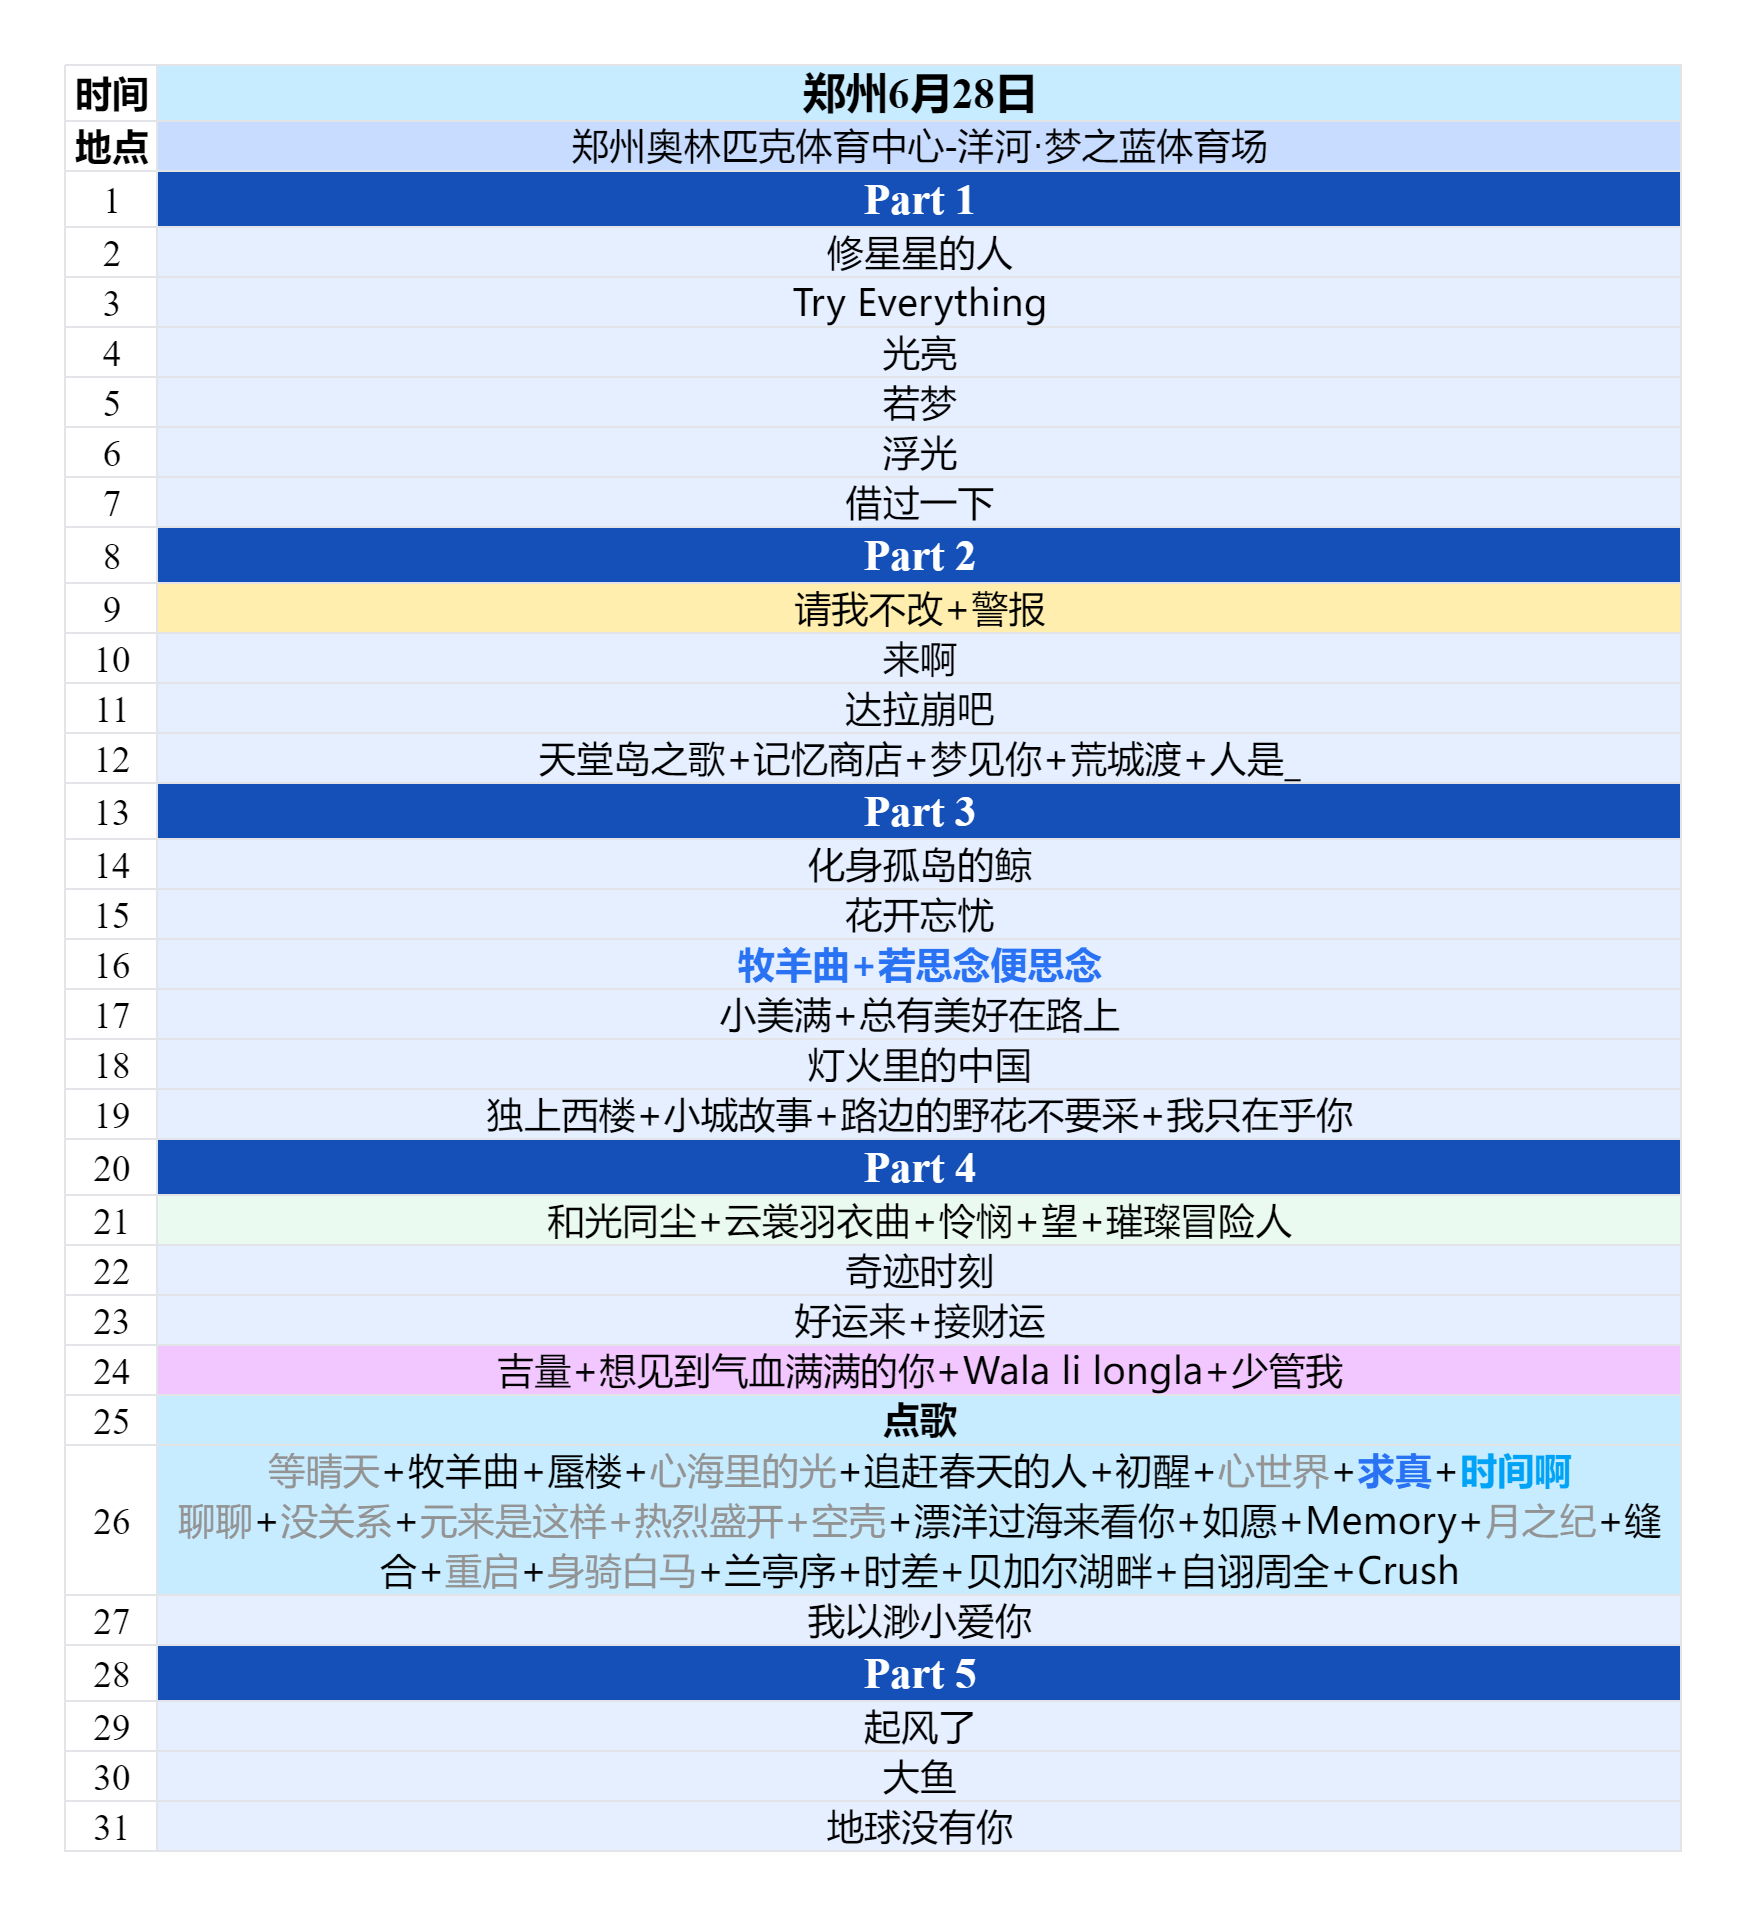
\includegraphics[width=280pt]{img/playlists/ZhengZhou-20260628} 

}

\caption{2026周深“深深的”巡回演唱会2026.06.28郑州场歌单}\label{fig:unnamed-chunk-24}
\end{figure}

\newpage

\section{Part1}\label{ZhengZhou-20260628-part1}

\hyperref[opening-vcr]{🎥【\textbf{开场VCR}】}

\hyperref[xiu-xing-xing-de-ren]{🎵【\textbf{修星星的人}】}

\hyperref[try-everything]{🎵【\textbf{Try Everything}】}

\hyperref[silver-linings]{🎵【\textbf{光亮}】}

\hyperref[like-a-dream]{🎵【\textbf{若梦}】}

\hyperref[floating-light]{🎵【\textbf{浮光}】}

\hyperref[excuse-me]{🎵【\textbf{借过一下}】}

\section{Part2}\label{ZhengZhou-20260628-part2}

\hyperref[robot-vcr]{🎥【\textbf{机器人VCR}】}

\hyperref[brave-heart]{🎵【\textbf{请我不改}】}

\hyperref[jing-bao]{🎵【\textbf{警报}】}

\hyperref[lai-a]{🎵【\textbf{来啊}】}

\hyperref[dalabengba]{🎵【\textbf{达拉崩吧}】}

\hyperref[haven-song]{🎵【\textbf{天堂岛之歌}】}

\hyperref[the-memory-store]{🎵【\textbf{记忆商店}】}

\hyperref[meng-jian-ni]{🎵【\textbf{梦见你}】}

\hyperref[huang-cheng-du]{🎵【\textbf{荒城渡}】}

\hyperref[Humans_are_]{🎵【\textbf{人是\_}】}

\section{Part3}\label{ZhengZhou-20260628-part3}

\hyperref[music-animations-vcr]{🎥【\textbf{音乐动画VCR}】}

\hyperref[The-whale-who-became-an-island]{🎵【\textbf{化身孤岛的鲸}】}

\hyperref[Blossoms-that-forget-sorrow]{🎵【\textbf{花开忘忧}】}

\hyperref[mu-yang-qu]{🎵【\textbf{牧羊曲}】}

\hyperref[ruo-si-nian-bian-si-nian]{🎵【\textbf{若思念便思念}】}

\hyperref[simple-bliss]{🎵【\textbf{小美满}】}

\hyperref[zong-you-mei-hao-zai-lu-shang]{🎵【\textbf{总有美好在路上}】}

\hyperref[deng-huo-li-de-zhong-guo]{🎵【\textbf{灯火里的中国}】}

🎵【\textbf{邓丽君组曲}】

\hyperref[du-shang-xi-lou]{🎵【\textbf{独上西楼}】}

\hyperref[xiao-cheng-gu-shi]{🎵【\textbf{小城故事}】}

\hyperref[donot-pick-the-roadside-flowers]{🎵【\textbf{路边的野花不要采}】}

\hyperref[I-only-care-about-you]{🎵【\textbf{我只在乎你}】}

\section{Part4}\label{ZhengZhou-20260628-part4}

\hyperref[mask-vcr]{🎥【\textbf{面具VCR}】}

\hyperref[stay-with-light]{🎵【\textbf{和光同尘}】}

\hyperref[Song-of-the-cloud-dress]{🎵【\textbf{云裳羽衣曲}】}

\hyperref[lian-min]{🎵【\textbf{怜悯}】}

\hyperref[Expectation]{🎵【\textbf{望}】}

\hyperref[adventurers]{🎵【\textbf{璀璨冒险人}】}

\hyperref[miracle-moment]{🎵【\textbf{奇迹时刻}】}

\hyperref[good-fortune-comes]{🎵【\textbf{好运来}】}

\hyperref[jie-cai-yun]{🎵【\textbf{接财运}】}

\hyperref[ji-liang]{🎵【\textbf{吉量}】}

\hyperref[xiang-jian-dao-qi-xue-man-man-de-ni]{🎵【\textbf{想见到气血满满的你}】}

\hyperref[wala-li-longla]{🎵【\textbf{Wala li longla}】}

\hyperref[watch-ur-manners]{🎵【\textbf{少管我}】}

【\textbf{点歌环节}】

\hyperref[qiu-zhen]{🎵【\textbf{求真}】}

\hyperref[shi-jian-a]{🎵【\textbf{时间啊}】}

\hyperref[loving-you-in-my-humble-way]{🎵【\textbf{我以渺小爱你}】}

\section{Part5}\label{ZhengZhou-20260628-part5}

\hyperref[exchange-diaries-vcr]{🎥【\textbf{交换日记VCR}】}

\hyperref[the-wind-rises]{🎵【\textbf{起风了}】}

\hyperref[big-fish]{🎵【\textbf{大鱼}】}

\hyperref[di-qiu-mei-you-ni]{🎵【\textbf{地球没有你}】}

\chapter{2026.07.11呼和浩特场 (WIP)}\label{HuHeHaoTe-20260711}

\begin{quote}
\begin{flushright}------周深\end{flushright}
\end{quote}

\begin{figure}

{\centering 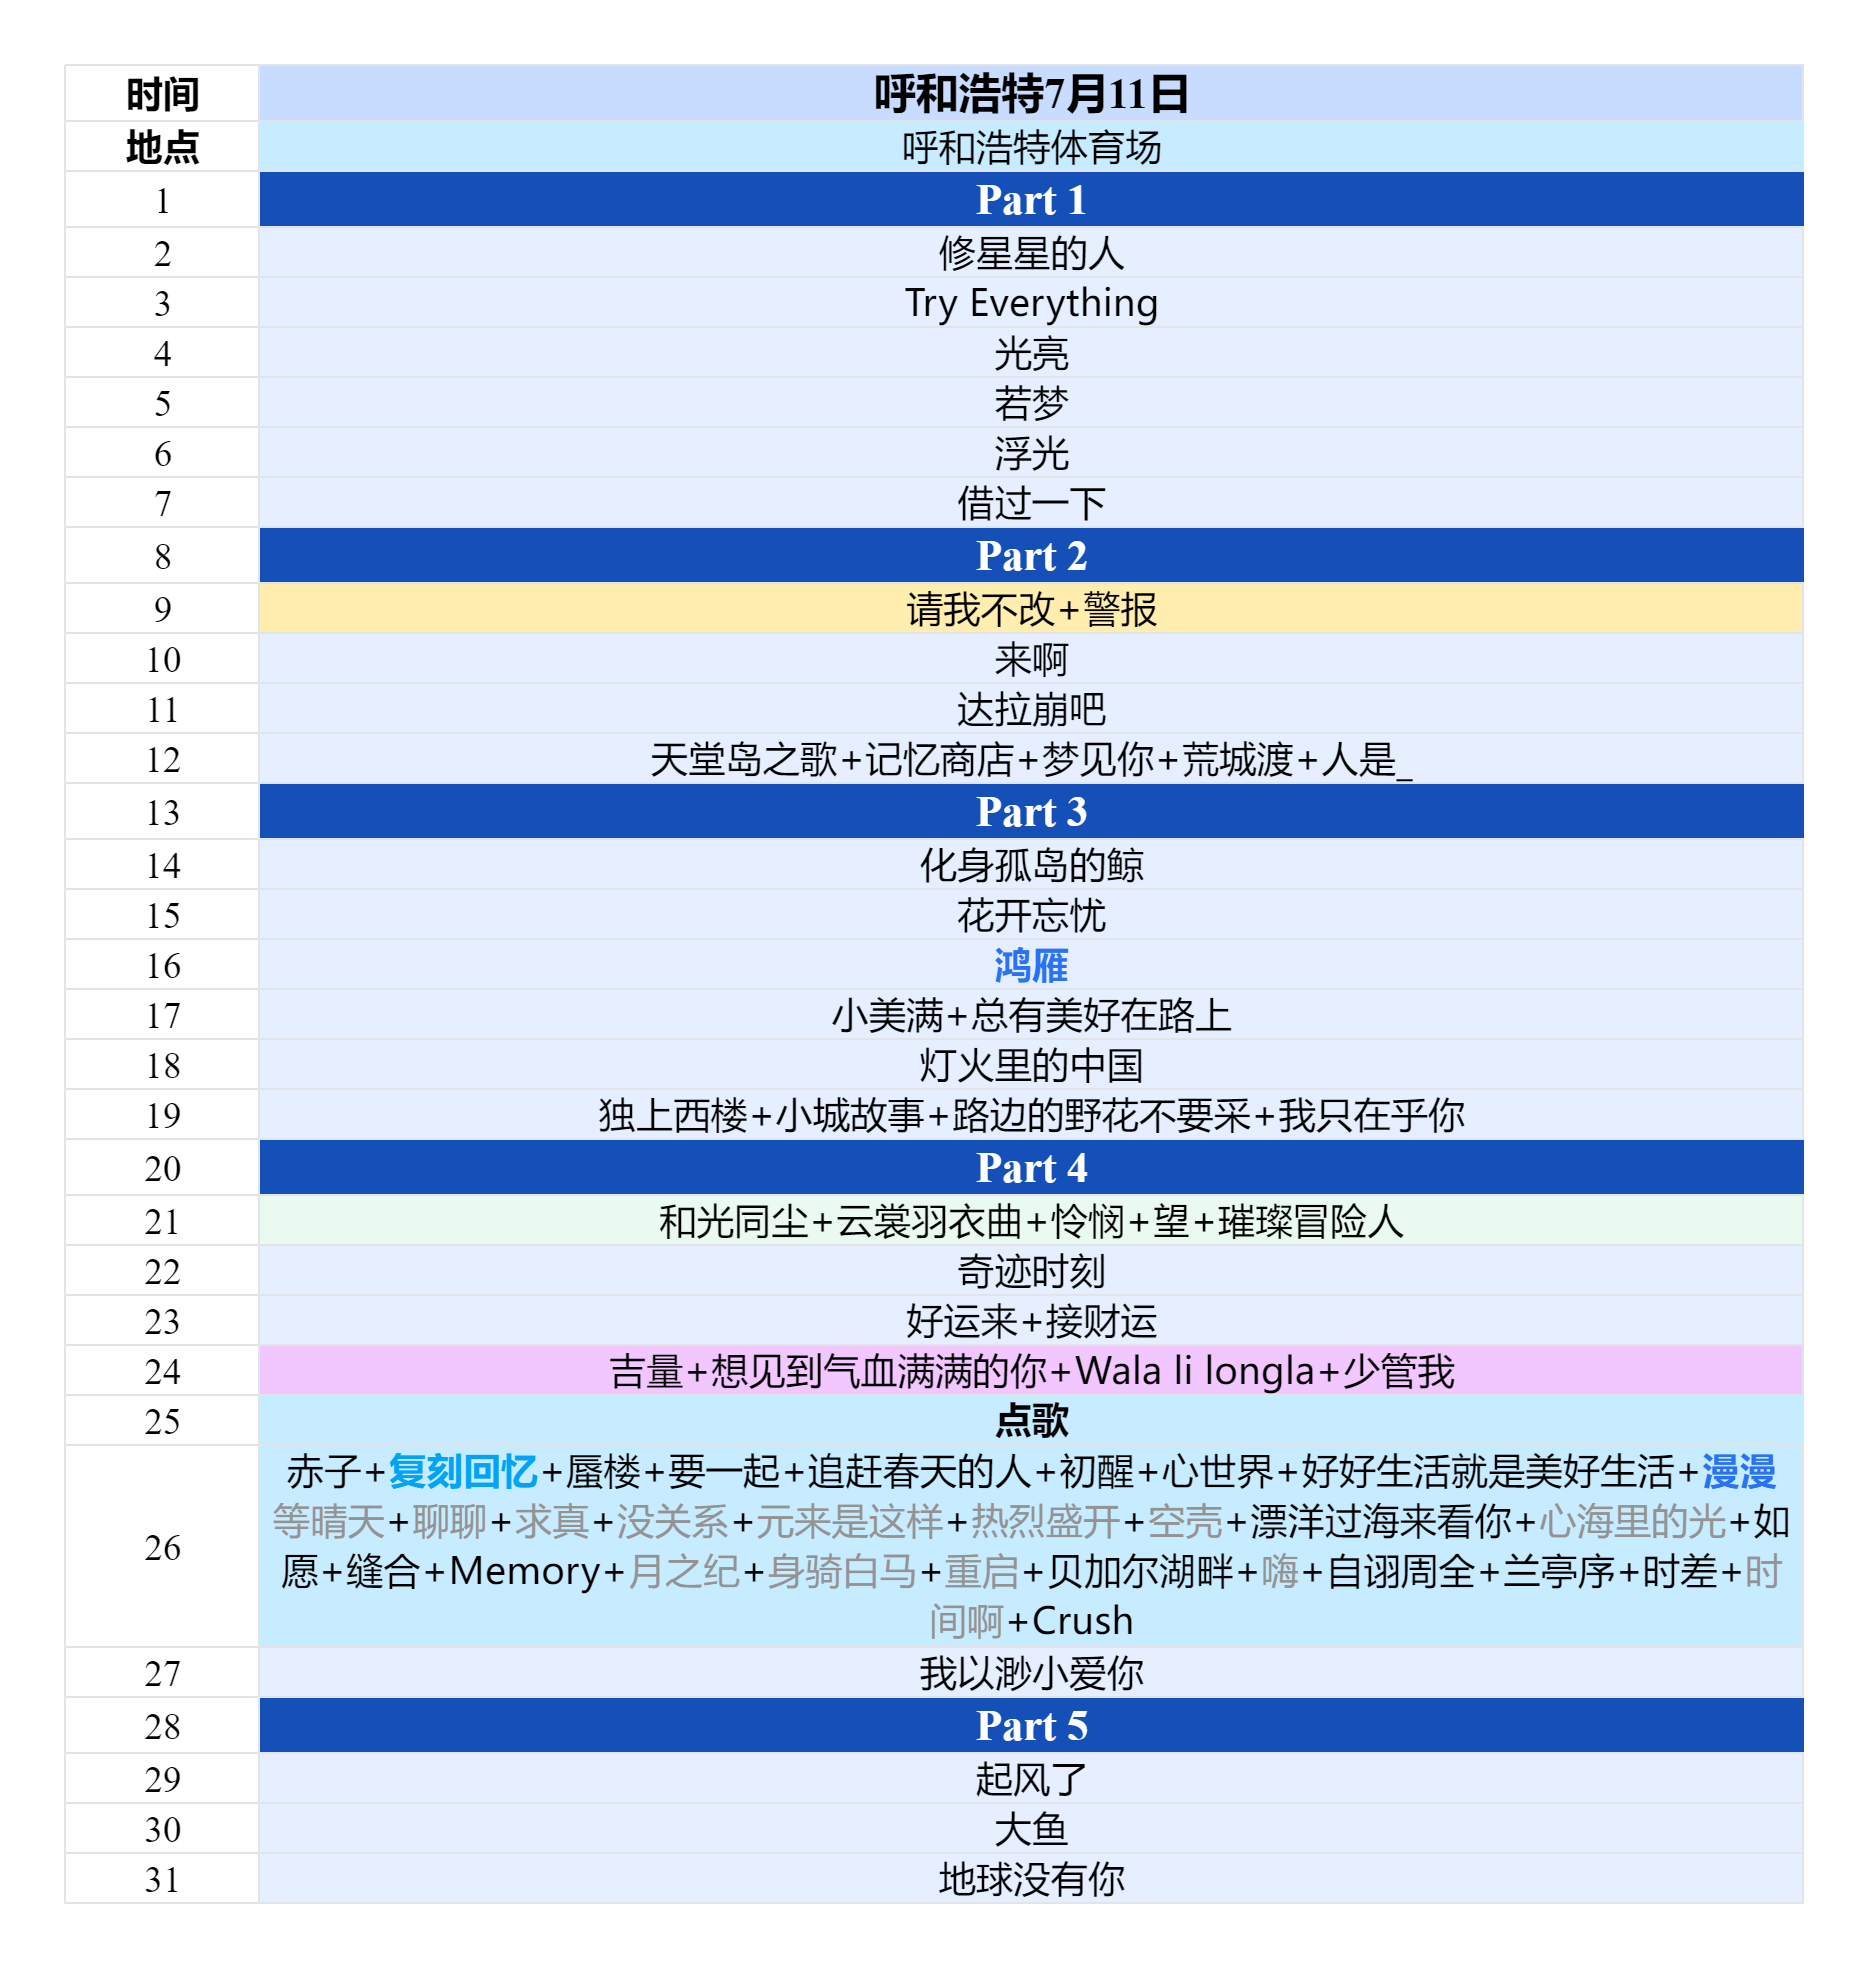
\includegraphics[width=280pt]{img/playlists/HuHeHaoTe-20260711} 

}

\caption{2026周深“深深的”巡回演唱会2026.07.11呼和浩特场歌单}\label{fig:unnamed-chunk-26}
\end{figure}

\newpage

\section{Part1}\label{HuHeHaoTe-20260711-part1}

\hyperref[opening-vcr]{🎥【\textbf{开场VCR}】}

\hyperref[xiu-xing-xing-de-ren]{🎵【\textbf{修星星的人}】}

\hyperref[try-everything]{🎵【\textbf{Try Everything}】}

\hyperref[silver-linings]{🎵【\textbf{光亮}】}

\hyperref[like-a-dream]{🎵【\textbf{若梦}】}

\hyperref[floating-light]{🎵【\textbf{浮光}】}

\hyperref[excuse-me]{🎵【\textbf{借过一下}】}

\section{Part2}\label{HuHeHaoTe-20260711-part2}

\hyperref[robot-vcr]{🎥【\textbf{机器人VCR}】}

\hyperref[brave-heart]{🎵【\textbf{请我不改}】}

\hyperref[jing-bao]{🎵【\textbf{警报}】}

\hyperref[lai-a]{🎵【\textbf{来啊}】}

\hyperref[dalabengba]{🎵【\textbf{达拉崩吧}】}

\hyperref[haven-song]{🎵【\textbf{天堂岛之歌}】}

\hyperref[the-memory-store]{🎵【\textbf{记忆商店}】}

\hyperref[meng-jian-ni]{🎵【\textbf{梦见你}】}

\hyperref[huang-cheng-du]{🎵【\textbf{荒城渡}】}

\hyperref[Humans_are_]{🎵【\textbf{人是\_}】}

\section{Part3}\label{HuHeHaoTe-20260711-part3}

\hyperref[music-animations-vcr]{🎥【\textbf{音乐动画VCR}】}

\hyperref[The-whale-who-became-an-island]{🎵【\textbf{化身孤岛的鲸}】}

\hyperref[Blossoms-that-forget-sorrow]{🎵【\textbf{花开忘忧}】}

\hyperref[hong-yan]{🎵【\textbf{鸿雁}】}

\hyperref[simple-bliss]{🎵【\textbf{小美满}】}

\hyperref[zong-you-mei-hao-zai-lu-shang]{🎵【\textbf{总有美好在路上}】}

\hyperref[deng-huo-li-de-zhong-guo]{🎵【\textbf{灯火里的中国}】}

🎵【\textbf{邓丽君组曲}】

\hyperref[du-shang-xi-lou]{🎵【\textbf{独上西楼}】}

\hyperref[xiao-cheng-gu-shi]{🎵【\textbf{小城故事}】}

\hyperref[donot-pick-the-roadside-flowers]{🎵【\textbf{路边的野花不要采}】}

\hyperref[I-only-care-about-you]{🎵【\textbf{我只在乎你}】}

\section{Part4}\label{HuHeHaoTe-20260711-part4}

\hyperref[mask-vcr]{🎥【\textbf{面具VCR}】}

\hyperref[stay-with-light]{🎵【\textbf{和光同尘}】}

\hyperref[Song-of-the-cloud-dress]{🎵【\textbf{云裳羽衣曲}】}

\hyperref[lian-min]{🎵【\textbf{怜悯}】}

\hyperref[Expectation]{🎵【\textbf{望}】}

\hyperref[adventurers]{🎵【\textbf{璀璨冒险人}】}

\hyperref[miracle-moment]{🎵【\textbf{奇迹时刻}】}

\hyperref[good-fortune-comes]{🎵【\textbf{好运来}】}

\hyperref[jie-cai-yun]{🎵【\textbf{接财运}】}

\hyperref[ji-liang]{🎵【\textbf{吉量}】}

\hyperref[xiang-jian-dao-qi-xue-man-man-de-ni]{🎵【\textbf{想见到气血满满的你}】}

\hyperref[wala-li-longla]{🎵【\textbf{Wala li longla}】}

\hyperref[watch-ur-manners]{🎵【\textbf{少管我}】}

【\textbf{点歌环节}】

\hyperref[man-man]{🎵【\textbf{漫漫}】}

\hyperref[fu-ke-hui-yi]{🎵【\textbf{复刻回忆}】}

\hyperref[loving-you-in-my-humble-way]{🎵【\textbf{我以渺小爱你}】}

\section{Part5}\label{HuHeHaoTe-20260711-part5}

\hyperref[exchange-diaries-vcr]{🎥【\textbf{交换日记VCR}】}

\hyperref[the-wind-rises]{🎵【\textbf{起风了}】}

\hyperref[big-fish]{🎵【\textbf{大鱼}】}

\hyperref[di-qiu-mei-you-ni]{🎵【\textbf{地球没有你}】}

\chapter{2026.07.12呼和浩特场 (WIP)}\label{HuHeHaoTe-20260712}

\begin{quote}
\begin{flushright}------周深\end{flushright}
\end{quote}

\begin{figure}

{\centering 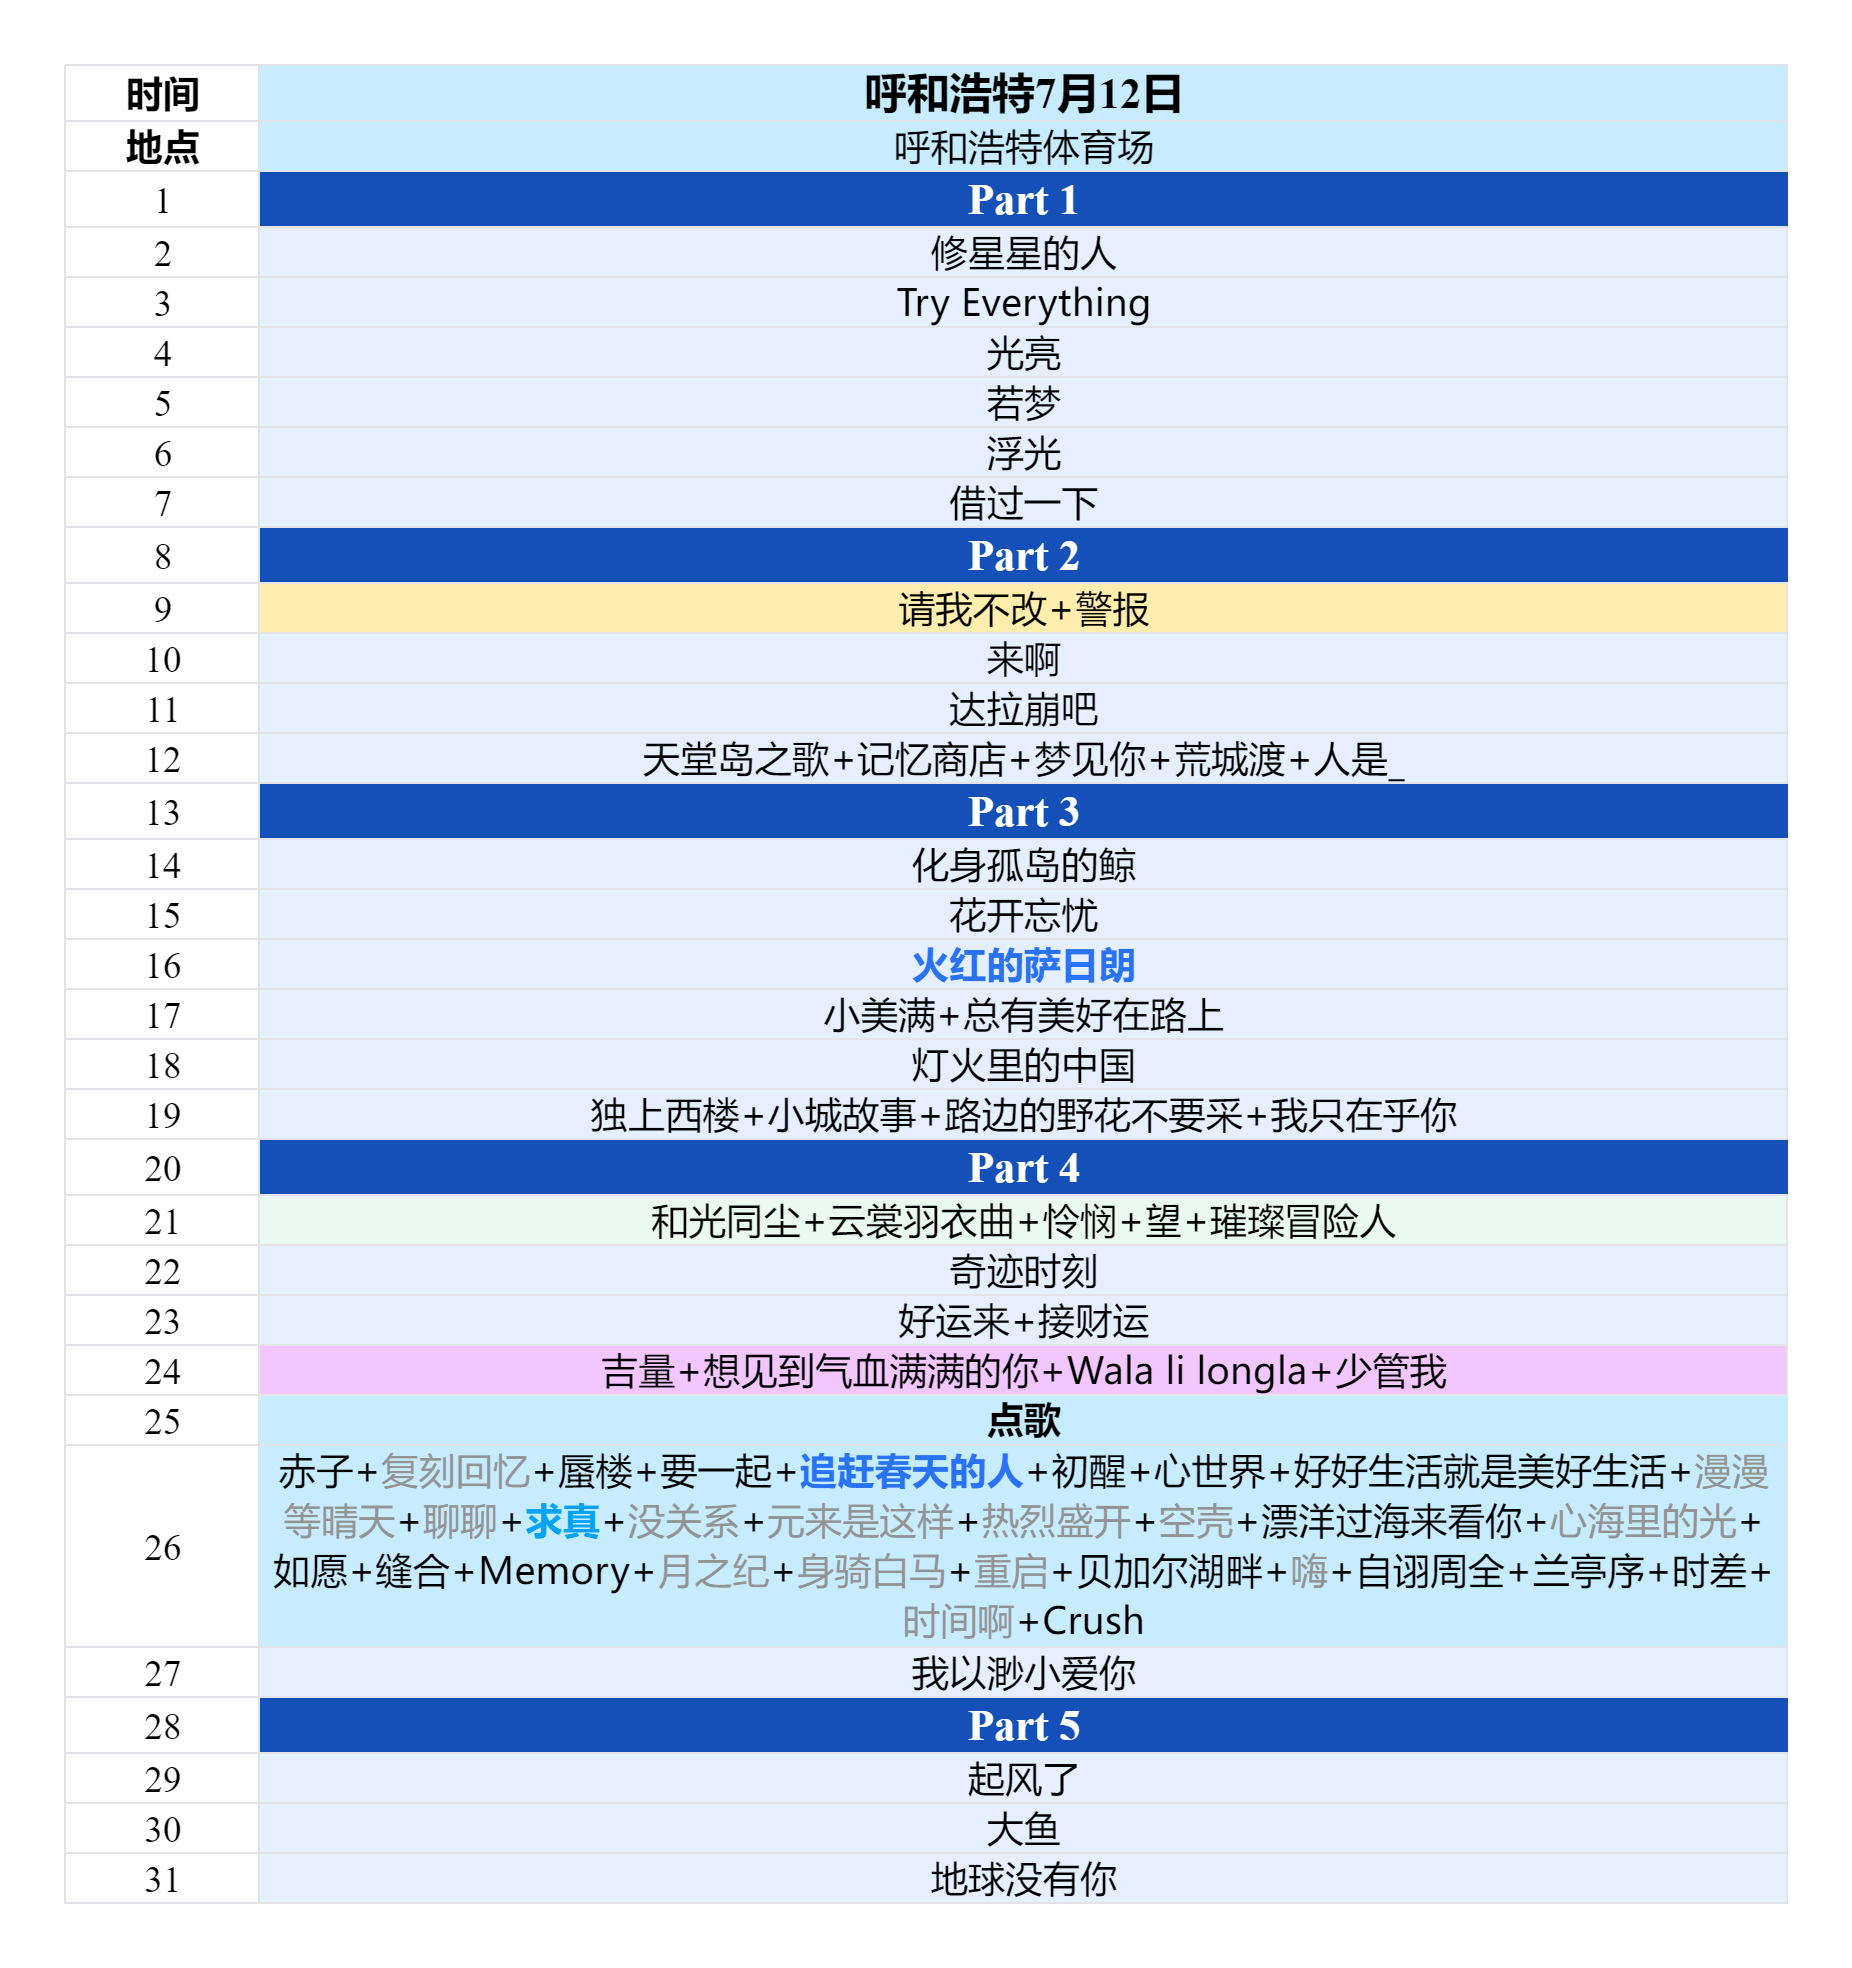
\includegraphics[width=280pt]{img/playlists/HuHeHaoTe-20260712} 

}

\caption{2026周深“深深的”巡回演唱会2026.07.12呼和浩特场歌单}\label{fig:unnamed-chunk-28}
\end{figure}

\newpage

\section{Part1}\label{HuHeHaoTe-20260712-part1}

\hyperref[opening-vcr]{🎥【\textbf{开场VCR}】}

\hyperref[xiu-xing-xing-de-ren]{🎵【\textbf{修星星的人}】}

\hyperref[try-everything]{🎵【\textbf{Try Everything}】}

\hyperref[silver-linings]{🎵【\textbf{光亮}】}

\hyperref[like-a-dream]{🎵【\textbf{若梦}】}

\hyperref[floating-light]{🎵【\textbf{浮光}】}

\hyperref[excuse-me]{🎵【\textbf{借过一下}】}

\section{Part2}\label{HuHeHaoTe-20260712-part2}

\hyperref[robot-vcr]{🎥【\textbf{机器人VCR}】}

\hyperref[brave-heart]{🎵【\textbf{请我不改}】}

\hyperref[jing-bao]{🎵【\textbf{警报}】}

\hyperref[lai-a]{🎵【\textbf{来啊}】}

\hyperref[dalabengba]{🎵【\textbf{达拉崩吧}】}

\hyperref[haven-song]{🎵【\textbf{天堂岛之歌}】}

\hyperref[the-memory-store]{🎵【\textbf{记忆商店}】}

\hyperref[meng-jian-ni]{🎵【\textbf{梦见你}】}

\hyperref[huang-cheng-du]{🎵【\textbf{荒城渡}】}

\hyperref[Humans_are_]{🎵【\textbf{人是\_}】}

\section{Part3}\label{HuHeHaoTe-20260712-part3}

\hyperref[music-animations-vcr]{🎥【\textbf{音乐动画VCR}】}

\hyperref[The-whale-who-became-an-island]{🎵【\textbf{化身孤岛的鲸}】}

\hyperref[Blossoms-that-forget-sorrow]{🎵【\textbf{花开忘忧}】}

\hyperref[huo-hong-de-sa-ri-lang]{🎵【\textbf{火红的萨日朗}】}

\hyperref[simple-bliss]{🎵【\textbf{小美满}】}

\hyperref[zong-you-mei-hao-zai-lu-shang]{🎵【\textbf{总有美好在路上}】}

\hyperref[deng-huo-li-de-zhong-guo]{🎵【\textbf{灯火里的中国}】}

🎵【\textbf{邓丽君组曲}】

\hyperref[du-shang-xi-lou]{🎵【\textbf{独上西楼}】}

\hyperref[xiao-cheng-gu-shi]{🎵【\textbf{小城故事}】}

\hyperref[donot-pick-the-roadside-flowers]{🎵【\textbf{路边的野花不要采}】}

\hyperref[I-only-care-about-you]{🎵【\textbf{我只在乎你}】}

\section{Part4}\label{HuHeHaoTe-20260712-part4}

\hyperref[mask-vcr]{🎥【\textbf{面具VCR}】}

\hyperref[stay-with-light]{🎵【\textbf{和光同尘}】}

\hyperref[Song-of-the-cloud-dress]{🎵【\textbf{云裳羽衣曲}】}

\hyperref[lian-min]{🎵【\textbf{怜悯}】}

\hyperref[Expectation]{🎵【\textbf{望}】}

\hyperref[adventurers]{🎵【\textbf{璀璨冒险人}】}

\hyperref[miracle-moment]{🎵【\textbf{奇迹时刻}】}

\hyperref[good-fortune-comes]{🎵【\textbf{好运来}】}

\hyperref[jie-cai-yun]{🎵【\textbf{接财运}】}

\hyperref[ji-liang]{🎵【\textbf{吉量}】}

\hyperref[xiang-jian-dao-qi-xue-man-man-de-ni]{🎵【\textbf{想见到气血满满的你}】}

\hyperref[wala-li-longla]{🎵【\textbf{Wala li longla}】}

\hyperref[watch-ur-manners]{🎵【\textbf{少管我}】}

【\textbf{点歌环节}】

\hyperref[zhui-gan-chun-tian-de-ren]{🎵【\textbf{追赶春天的人}】}

\hyperref[qiu-zhen]{🎵【\textbf{求真}】}

\hyperref[loving-you-in-my-humble-way]{🎵【\textbf{我以渺小爱你}】}

\section{Part5}\label{HuHeHaoTe-20260712-part5}

\hyperref[exchange-diaries-vcr]{🎥【\textbf{交换日记VCR}】}

\hyperref[the-wind-rises]{🎵【\textbf{起风了}】}

\hyperref[big-fish]{🎵【\textbf{大鱼}】}

\hyperref[di-qiu-mei-you-ni]{🎵【\textbf{地球没有你}】}

\chapter{2026.07.25沈阳场 (WIP)}\label{ShenYang-20260725}

\begin{quote}
\begin{flushright}------周深\end{flushright}
\end{quote}

\begin{figure}

{\centering 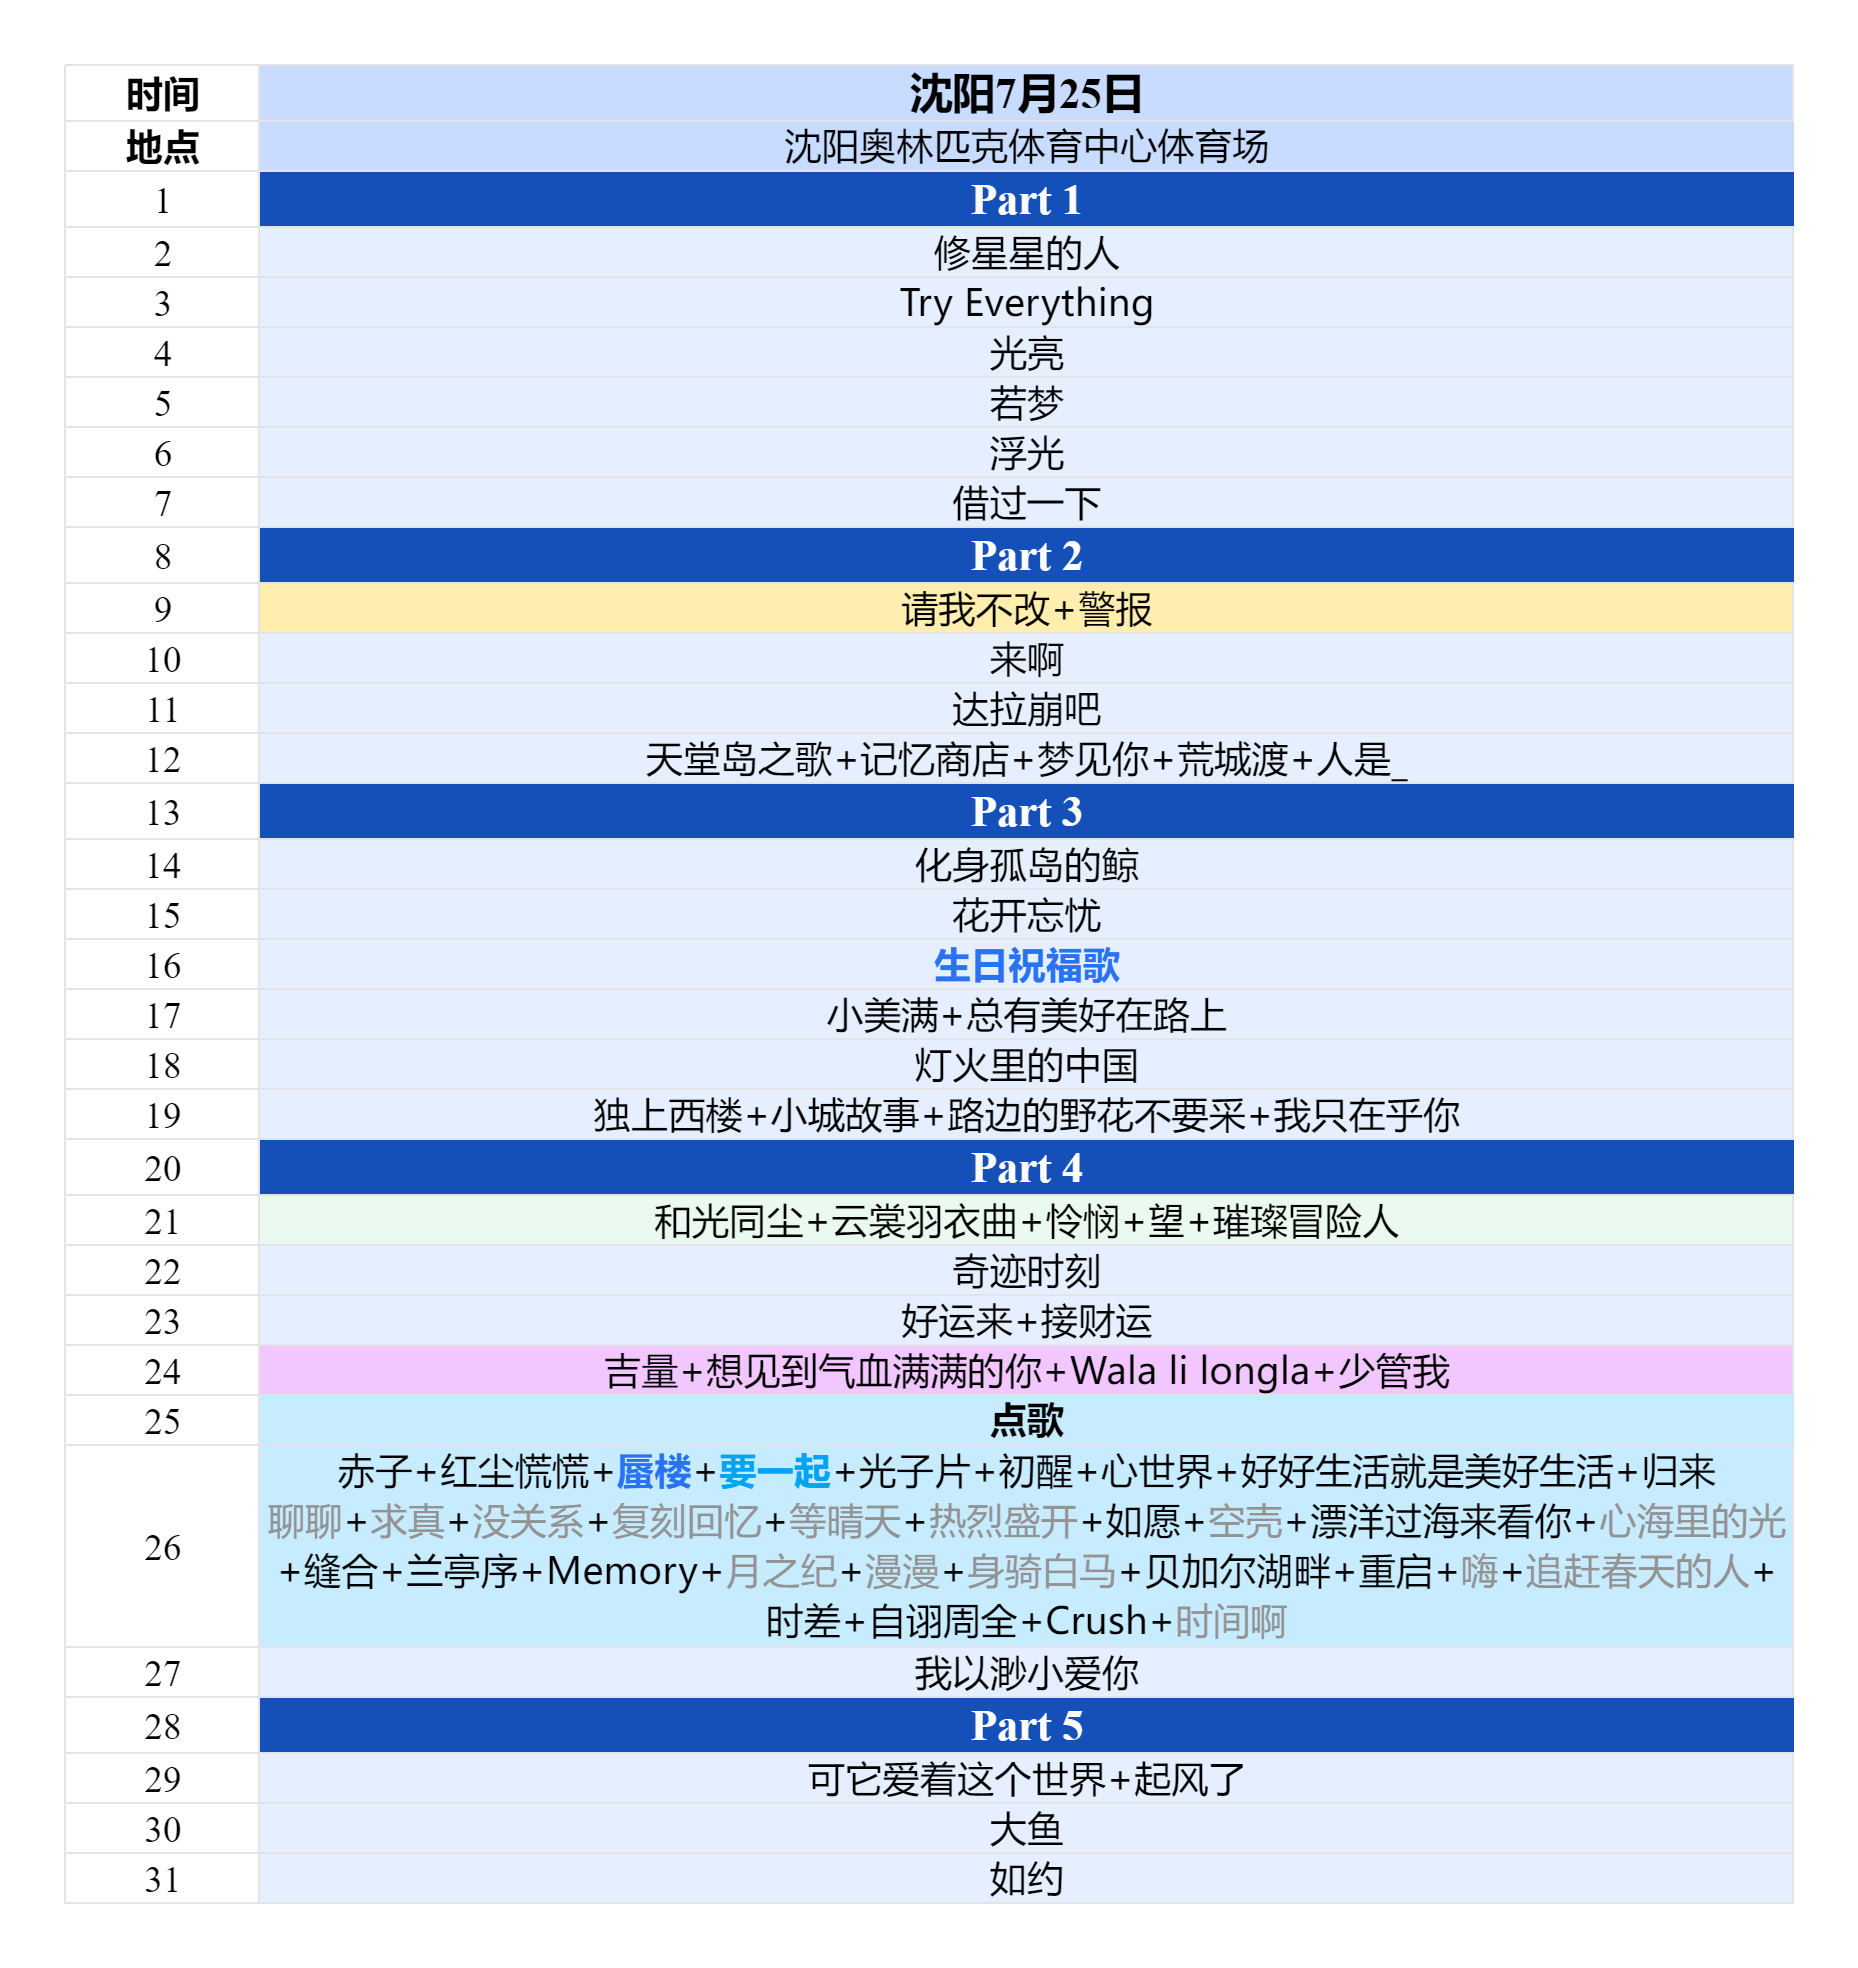
\includegraphics[width=280pt]{img/playlists/ShenYang-20260725} 

}

\caption{2026周深“深深的”巡回演唱会2026.07.25沈阳场歌单}\label{fig:unnamed-chunk-30}
\end{figure}

\newpage

\section{Part1}\label{ShenYang-20260725-part1}

\hyperref[opening-vcr]{🎥【\textbf{开场VCR}】}

\hyperref[xiu-xing-xing-de-ren]{🎵【\textbf{修星星的人}】}

\hyperref[try-everything]{🎵【\textbf{Try Everything}】}

\hyperref[silver-linings]{🎵【\textbf{光亮}】}

\hyperref[like-a-dream]{🎵【\textbf{若梦}】}

\hyperref[floating-light]{🎵【\textbf{浮光}】}

\hyperref[excuse-me]{🎵【\textbf{借过一下}】}

\section{Part2}\label{ShenYang-20260725-part2}

\hyperref[robot-vcr]{🎥【\textbf{机器人VCR}】}

\hyperref[brave-heart]{🎵【\textbf{请我不改}】}

\hyperref[jing-bao]{🎵【\textbf{警报}】}

\hyperref[lai-a]{🎵【\textbf{来啊}】}

\hyperref[dalabengba]{🎵【\textbf{达拉崩吧}】}

\hyperref[haven-song]{🎵【\textbf{天堂岛之歌}】}

\hyperref[the-memory-store]{🎵【\textbf{记忆商店}】}

\hyperref[meng-jian-ni]{🎵【\textbf{梦见你}】}

\hyperref[huang-cheng-du]{🎵【\textbf{荒城渡}】}

\hyperref[Humans_are_]{🎵【\textbf{人是\_}】}

\section{Part3}\label{ShenYang-20260725-part3}

\hyperref[music-animations-vcr]{🎥【\textbf{音乐动画VCR}】}

\hyperref[The-whale-who-became-an-island]{🎵【\textbf{化身孤岛的鲸}】}

\hyperref[Blossoms-that-forget-sorrow]{🎵【\textbf{花开忘忧}】}

\hyperref[happy-birthday]{🎵【\textbf{生日祝福歌}】}

\hyperref[simple-bliss]{🎵【\textbf{小美满}】}

\hyperref[zong-you-mei-hao-zai-lu-shang]{🎵【\textbf{总有美好在路上}】}

\hyperref[deng-huo-li-de-zhong-guo]{🎵【\textbf{灯火里的中国}】}

🎵【\textbf{邓丽君组曲}】

\hyperref[du-shang-xi-lou]{🎵【\textbf{独上西楼}】}

\hyperref[xiao-cheng-gu-shi]{🎵【\textbf{小城故事}】}

\hyperref[donot-pick-the-roadside-flowers]{🎵【\textbf{路边的野花不要采}】}

\hyperref[I-only-care-about-you]{🎵【\textbf{我只在乎你}】}

\section{Part4}\label{ShenYang-20260725-part4}

\hyperref[mask-vcr]{🎥【\textbf{面具VCR}】}

\hyperref[stay-with-light]{🎵【\textbf{和光同尘}】}

\hyperref[Song-of-the-cloud-dress]{🎵【\textbf{云裳羽衣曲}】}

\hyperref[lian-min]{🎵【\textbf{怜悯}】}

\hyperref[Expectation]{🎵【\textbf{望}】}

\hyperref[adventurers]{🎵【\textbf{璀璨冒险人}】}

\hyperref[miracle-moment]{🎵【\textbf{奇迹时刻}】}

\hyperref[good-fortune-comes]{🎵【\textbf{好运来}】}

\hyperref[jie-cai-yun]{🎵【\textbf{接财运}】}

\hyperref[ji-liang]{🎵【\textbf{吉量}】}

\hyperref[xiang-jian-dao-qi-xue-man-man-de-ni]{🎵【\textbf{想见到气血满满的你}】}

\hyperref[wala-li-longla]{🎵【\textbf{Wala li longla}】}

\hyperref[watch-ur-manners]{🎵【\textbf{少管我}】}

【\textbf{点歌环节}】

\hyperref[mirage]{🎵【\textbf{蜃楼}】}

\hyperref[yao-yi-qi]{🎵【\textbf{要一起}】}

\hyperref[loving-you-in-my-humble-way]{🎵【\textbf{我以渺小爱你}】}

\section{Part5}\label{ShenYang-20260725-part5}

\hyperref[exchange-diaries-vcr]{🎥【\textbf{交换日记VCR}】}

\hyperref[ke-ta-ai-zhe-zhe-ge-shi-jie]{🎵【\textbf{可它爱着这个世界}】}

\hyperref[the-wind-rises]{🎵【\textbf{起风了}】}

\hyperref[big-fish]{🎵【\textbf{大鱼}】}

\hyperref[ru-yue]{🎵【\textbf{如约}】}

\chapter{2026.07.26沈阳场 (WIP)}\label{ShenYang-20260726}

\begin{quote}
\begin{flushright}------周深\end{flushright}
\end{quote}

\begin{figure}

{\centering 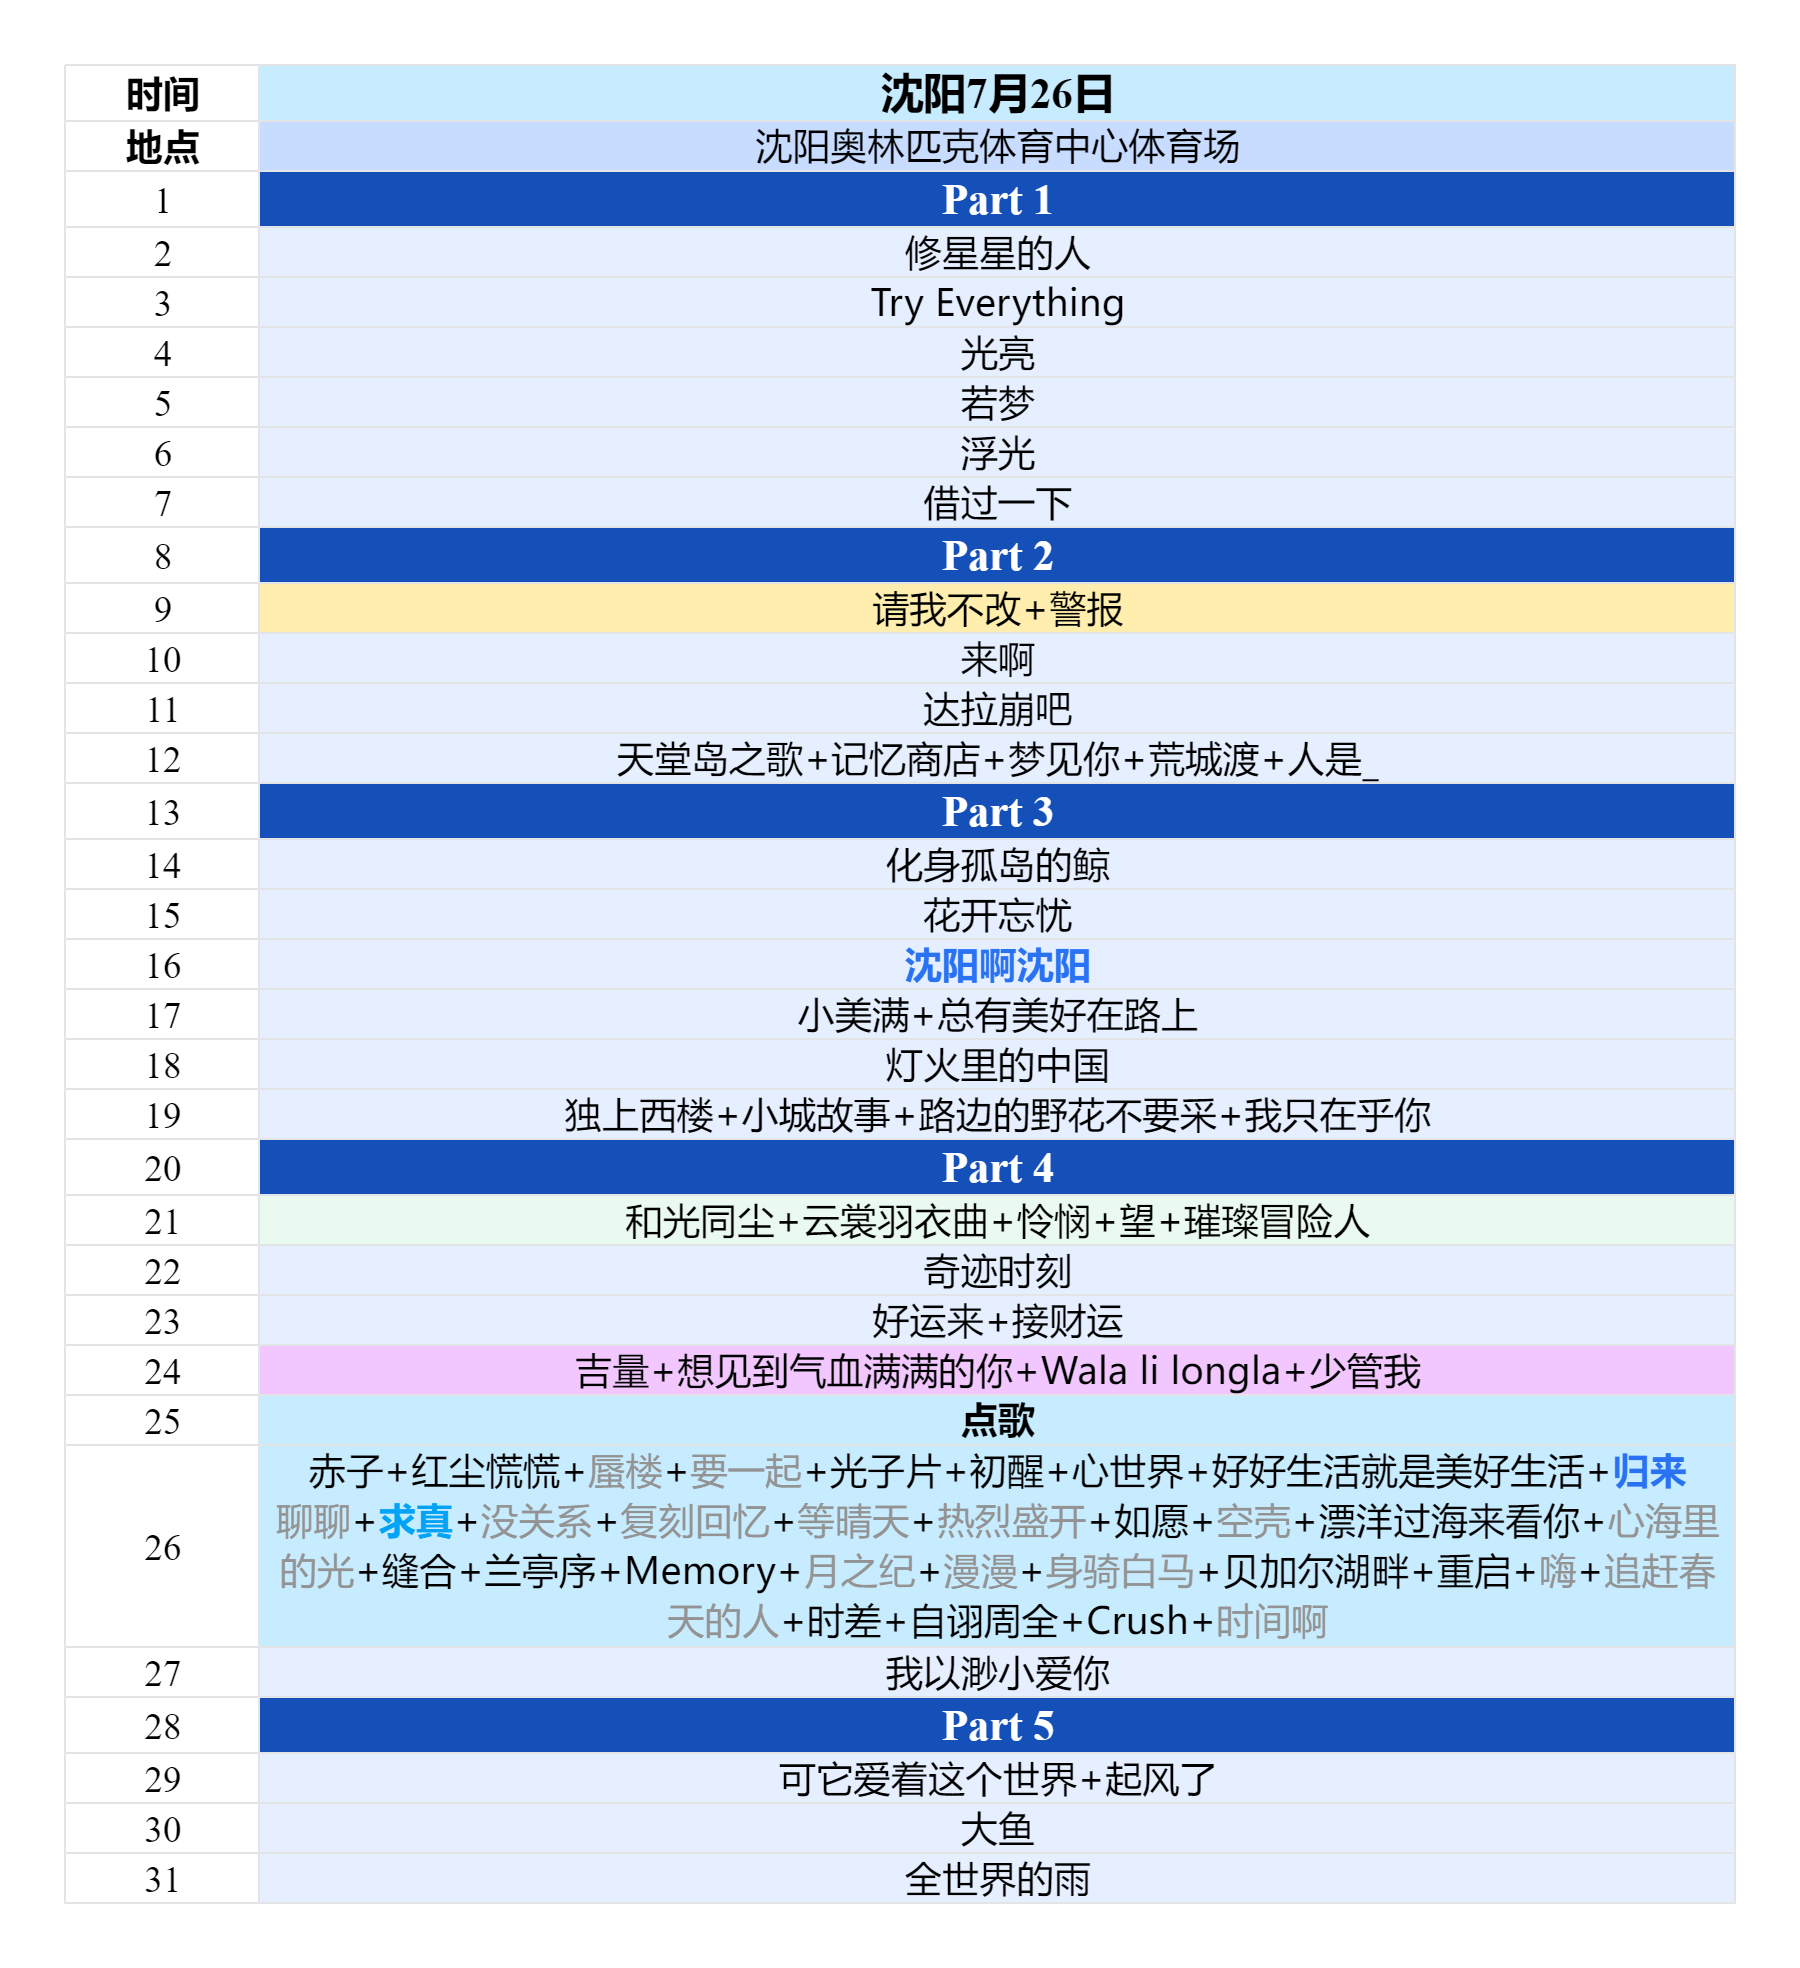
\includegraphics[width=280pt]{img/playlists/ShenYang-20260726} 

}

\caption{2026周深“深深的”巡回演唱会2026.07.26沈阳场歌单}\label{fig:unnamed-chunk-32}
\end{figure}

\newpage

\section{Part1}\label{ShenYang-20260726-part1}

\hyperref[opening-vcr]{🎥【\textbf{开场VCR}】}

\hyperref[xiu-xing-xing-de-ren]{🎵【\textbf{修星星的人}】}

\hyperref[try-everything]{🎵【\textbf{Try Everything}】}

\hyperref[silver-linings]{🎵【\textbf{光亮}】}

\hyperref[like-a-dream]{🎵【\textbf{若梦}】}

\hyperref[floating-light]{🎵【\textbf{浮光}】}

\hyperref[excuse-me]{🎵【\textbf{借过一下}】}

\section{Part2}\label{ShenYang-20260726-part2}

\hyperref[robot-vcr]{🎥【\textbf{机器人VCR}】}

\hyperref[brave-heart]{🎵【\textbf{请我不改}】}

\hyperref[jing-bao]{🎵【\textbf{警报}】}

\hyperref[lai-a]{🎵【\textbf{来啊}】}

\hyperref[dalabengba]{🎵【\textbf{达拉崩吧}】}

\hyperref[haven-song]{🎵【\textbf{天堂岛之歌}】}

\hyperref[the-memory-store]{🎵【\textbf{记忆商店}】}

\hyperref[meng-jian-ni]{🎵【\textbf{梦见你}】}

\hyperref[huang-cheng-du]{🎵【\textbf{荒城渡}】}

\hyperref[Humans_are_]{🎵【\textbf{人是\_}】}

\section{Part3}\label{ShenYang-20260726-part3}

\hyperref[music-animations-vcr]{🎥【\textbf{音乐动画VCR}】}

\hyperref[The-whale-who-became-an-island]{🎵【\textbf{化身孤岛的鲸}】}

\hyperref[Blossoms-that-forget-sorrow]{🎵【\textbf{花开忘忧}】}

\hyperref[shen-yang-a-shen-yang]{🎵【\textbf{沈阳啊沈阳}】}

\hyperref[simple-bliss]{🎵【\textbf{小美满}】}

\hyperref[zong-you-mei-hao-zai-lu-shang]{🎵【\textbf{总有美好在路上}】}

\hyperref[deng-huo-li-de-zhong-guo]{🎵【\textbf{灯火里的中国}】}

🎵【\textbf{邓丽君组曲}】

\hyperref[du-shang-xi-lou]{🎵【\textbf{独上西楼}】}

\hyperref[xiao-cheng-gu-shi]{🎵【\textbf{小城故事}】}

\hyperref[donot-pick-the-roadside-flowers]{🎵【\textbf{路边的野花不要采}】}

\hyperref[I-only-care-about-you]{🎵【\textbf{我只在乎你}】}

\section{Part4}\label{ShenYang-20260726-part4}

\hyperref[mask-vcr]{🎥【\textbf{面具VCR}】}

\hyperref[stay-with-light]{🎵【\textbf{和光同尘}】}

\hyperref[Song-of-the-cloud-dress]{🎵【\textbf{云裳羽衣曲}】}

\hyperref[lian-min]{🎵【\textbf{怜悯}】}

\hyperref[Expectation]{🎵【\textbf{望}】}

\hyperref[adventurers]{🎵【\textbf{璀璨冒险人}】}

\hyperref[miracle-moment]{🎵【\textbf{奇迹时刻}】}

\hyperref[good-fortune-comes]{🎵【\textbf{好运来}】}

\hyperref[jie-cai-yun]{🎵【\textbf{接财运}】}

\hyperref[ji-liang]{🎵【\textbf{吉量}】}

\hyperref[xiang-jian-dao-qi-xue-man-man-de-ni]{🎵【\textbf{想见到气血满满的你}】}

\hyperref[wala-li-longla]{🎵【\textbf{Wala li longla}】}

\hyperref[watch-ur-manners]{🎵【\textbf{少管我}】}

【\textbf{点歌环节}】

\hyperref[gui-lai]{🎵【\textbf{归来}】}

\hyperref[qiu-zhen]{🎵【\textbf{求真}】}

\hyperref[loving-you-in-my-humble-way]{🎵【\textbf{我以渺小爱你}】}

\section{Part5}\label{ShenYang-20260726-part5}

\hyperref[exchange-diaries-vcr]{🎥【\textbf{交换日记VCR}】}

\hyperref[ke-ta-ai-zhe-zhe-ge-shi-jie]{🎵【\textbf{可它爱着这个世界}】}

\hyperref[the-wind-rises]{🎵【\textbf{起风了}】}

\hyperref[big-fish]{🎵【\textbf{大鱼}】}

\hyperref[quan-shi-jie-de-yu]{🎵【\textbf{全世界的雨}】}

\chapter{2026.08.08贵阳场 (WIP)}\label{GuiYang-20260808}

\begin{quote}
\begin{flushright}------周深\end{flushright}
\end{quote}

\begin{figure}

{\centering 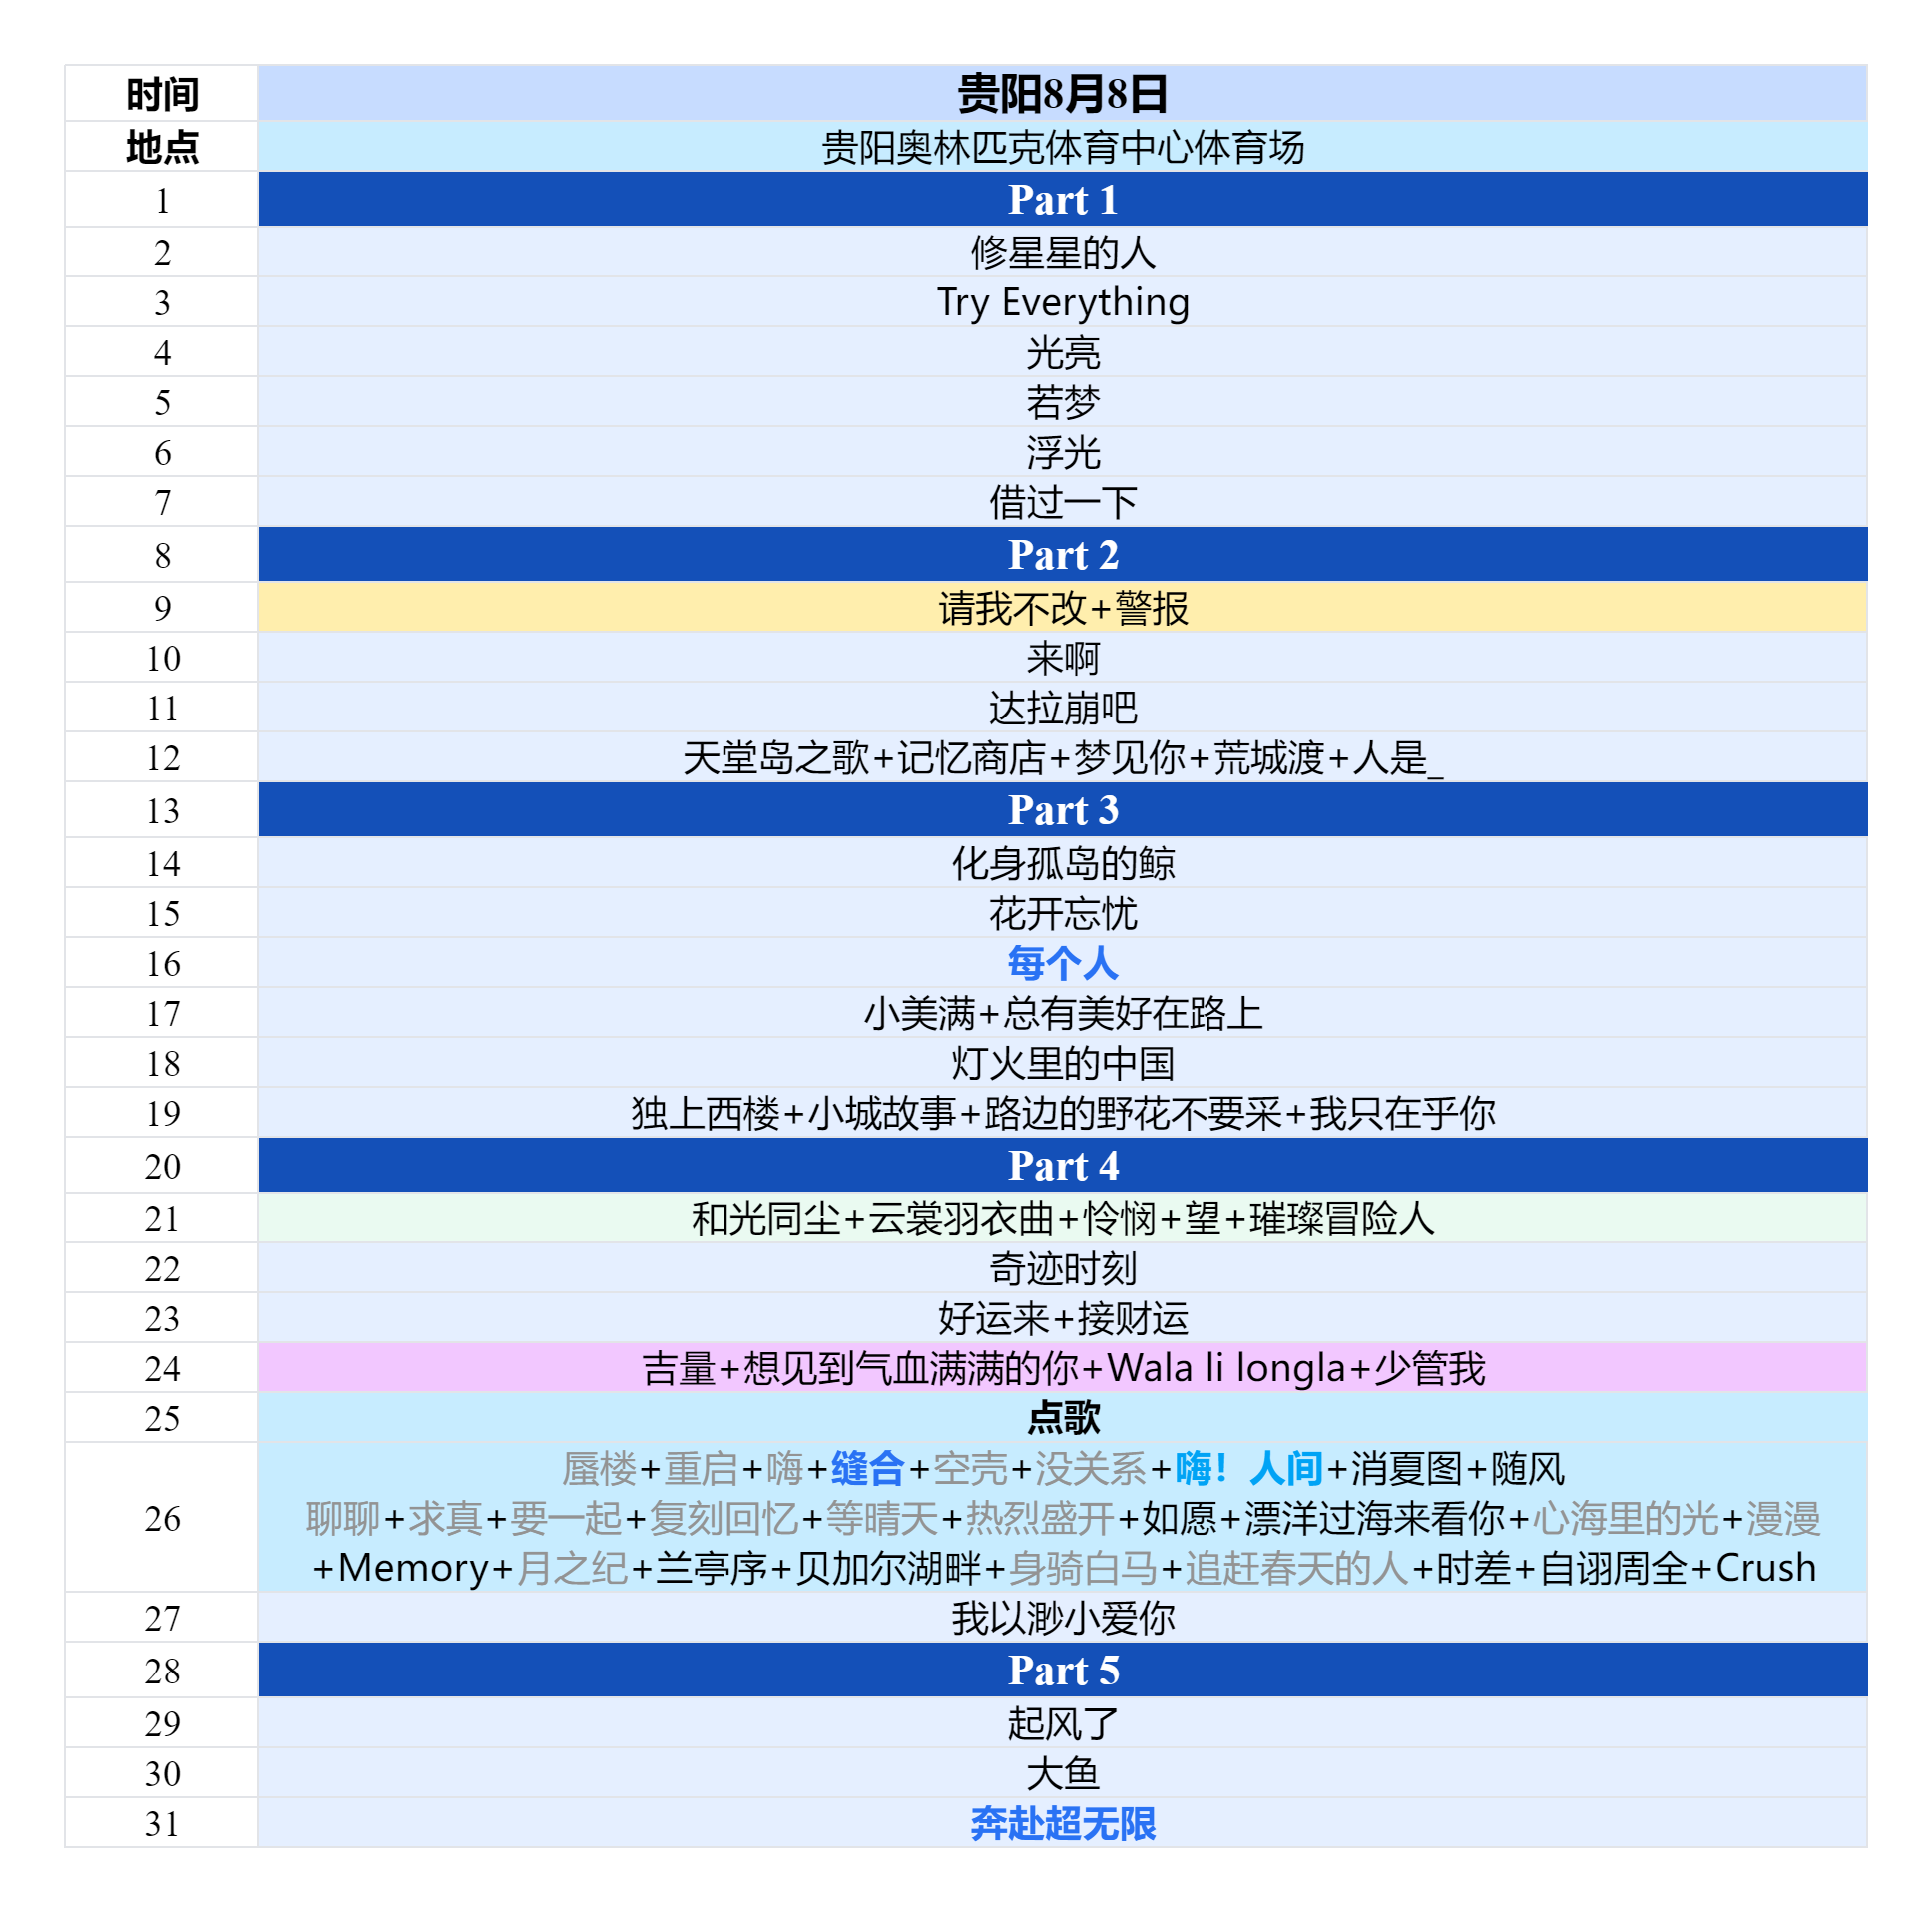
\includegraphics[width=280pt]{img/playlists/GuiYang-20260808} 

}

\caption{2026周深“深深的”巡回演唱会2026.08.08贵阳场歌单}\label{fig:unnamed-chunk-34}
\end{figure}

\newpage

\section{Part1}\label{GuiYang-20260808-part1}

\hyperref[opening-vcr]{🎥【\textbf{开场VCR}】}

\hyperref[xiu-xing-xing-de-ren]{🎵【\textbf{修星星的人}】}

\hyperref[try-everything]{🎵【\textbf{Try Everything}】}

\hyperref[silver-linings]{🎵【\textbf{光亮}】}

\hyperref[like-a-dream]{🎵【\textbf{若梦}】}

\hyperref[floating-light]{🎵【\textbf{浮光}】}

\hyperref[excuse-me]{🎵【\textbf{借过一下}】}

\section{Part2}\label{GuiYang-20260808-part2}

\hyperref[robot-vcr]{🎥【\textbf{机器人VCR}】}

\hyperref[brave-heart]{🎵【\textbf{请我不改}】}

\hyperref[jing-bao]{🎵【\textbf{警报}】}

\hyperref[lai-a]{🎵【\textbf{来啊}】}

\hyperref[dalabengba]{🎵【\textbf{达拉崩吧}】}

\hyperref[haven-song]{🎵【\textbf{天堂岛之歌}】}

\hyperref[the-memory-store]{🎵【\textbf{记忆商店}】}

\hyperref[meng-jian-ni]{🎵【\textbf{梦见你}】}

\hyperref[huang-cheng-du]{🎵【\textbf{荒城渡}】}

\hyperref[Humans_are_]{🎵【\textbf{人是\_}】}

\section{Part3}\label{GuiYang-20260808-part3}

\hyperref[music-animations-vcr]{🎥【\textbf{音乐动画VCR}】}

\hyperref[The-whale-who-became-an-island]{🎵【\textbf{化身孤岛的鲸}】}

\hyperref[Blossoms-that-forget-sorrow]{🎵【\textbf{花开忘忧}】}

\hyperref[mei-ge-ren]{🎵【\textbf{每个人}】}

\hyperref[simple-bliss]{🎵【\textbf{小美满}】}

\hyperref[zong-you-mei-hao-zai-lu-shang]{🎵【\textbf{总有美好在路上}】}

\hyperref[deng-huo-li-de-zhong-guo]{🎵【\textbf{灯火里的中国}】}

🎵【\textbf{邓丽君组曲}】

\hyperref[du-shang-xi-lou]{🎵【\textbf{独上西楼}】}

\hyperref[xiao-cheng-gu-shi]{🎵【\textbf{小城故事}】}

\hyperref[donot-pick-the-roadside-flowers]{🎵【\textbf{路边的野花不要采}】}

\hyperref[I-only-care-about-you]{🎵【\textbf{我只在乎你}】}

\section{Part4}\label{GuiYang-20260808-part4}

\hyperref[mask-vcr]{🎥【\textbf{面具VCR}】}

\hyperref[stay-with-light]{🎵【\textbf{和光同尘}】}

\hyperref[Song-of-the-cloud-dress]{🎵【\textbf{云裳羽衣曲}】}

\hyperref[lian-min]{🎵【\textbf{怜悯}】}

\hyperref[Expectation]{🎵【\textbf{望}】}

\hyperref[adventurers]{🎵【\textbf{璀璨冒险人}】}

\hyperref[miracle-moment]{🎵【\textbf{奇迹时刻}】}

\hyperref[good-fortune-comes]{🎵【\textbf{好运来}】}

\hyperref[jie-cai-yun]{🎵【\textbf{接财运}】}

\hyperref[ji-liang]{🎵【\textbf{吉量}】}

\hyperref[xiang-jian-dao-qi-xue-man-man-de-ni]{🎵【\textbf{想见到气血满满的你}】}

\hyperref[wala-li-longla]{🎵【\textbf{Wala li longla}】}

\hyperref[watch-ur-manners]{🎵【\textbf{少管我}】}

【\textbf{点歌环节}】

\hyperref[feng-he]{🎵【\textbf{缝合}】}

\hyperref[hello-world]{🎵【\textbf{嗨！人间}】}

\hyperref[loving-you-in-my-humble-way]{🎵【\textbf{我以渺小爱你}】}

\section{Part5}\label{GuiYang-20260808-part5}

\hyperref[exchange-diaries-vcr]{🎥【\textbf{交换日记VCR}】}

\hyperref[the-wind-rises]{🎵【\textbf{起风了}】}

\hyperref[big-fish]{🎵【\textbf{大鱼}】}

\hyperref[ben-fu-chao-wu-xian]{🎵【\textbf{奔赴超无限}】}

\chapter{2026.08.09贵阳场 (WIP)}\label{GuiYang-20260809}

\begin{quote}
\begin{flushright}------周深\end{flushright}
\end{quote}

\begin{figure}

{\centering 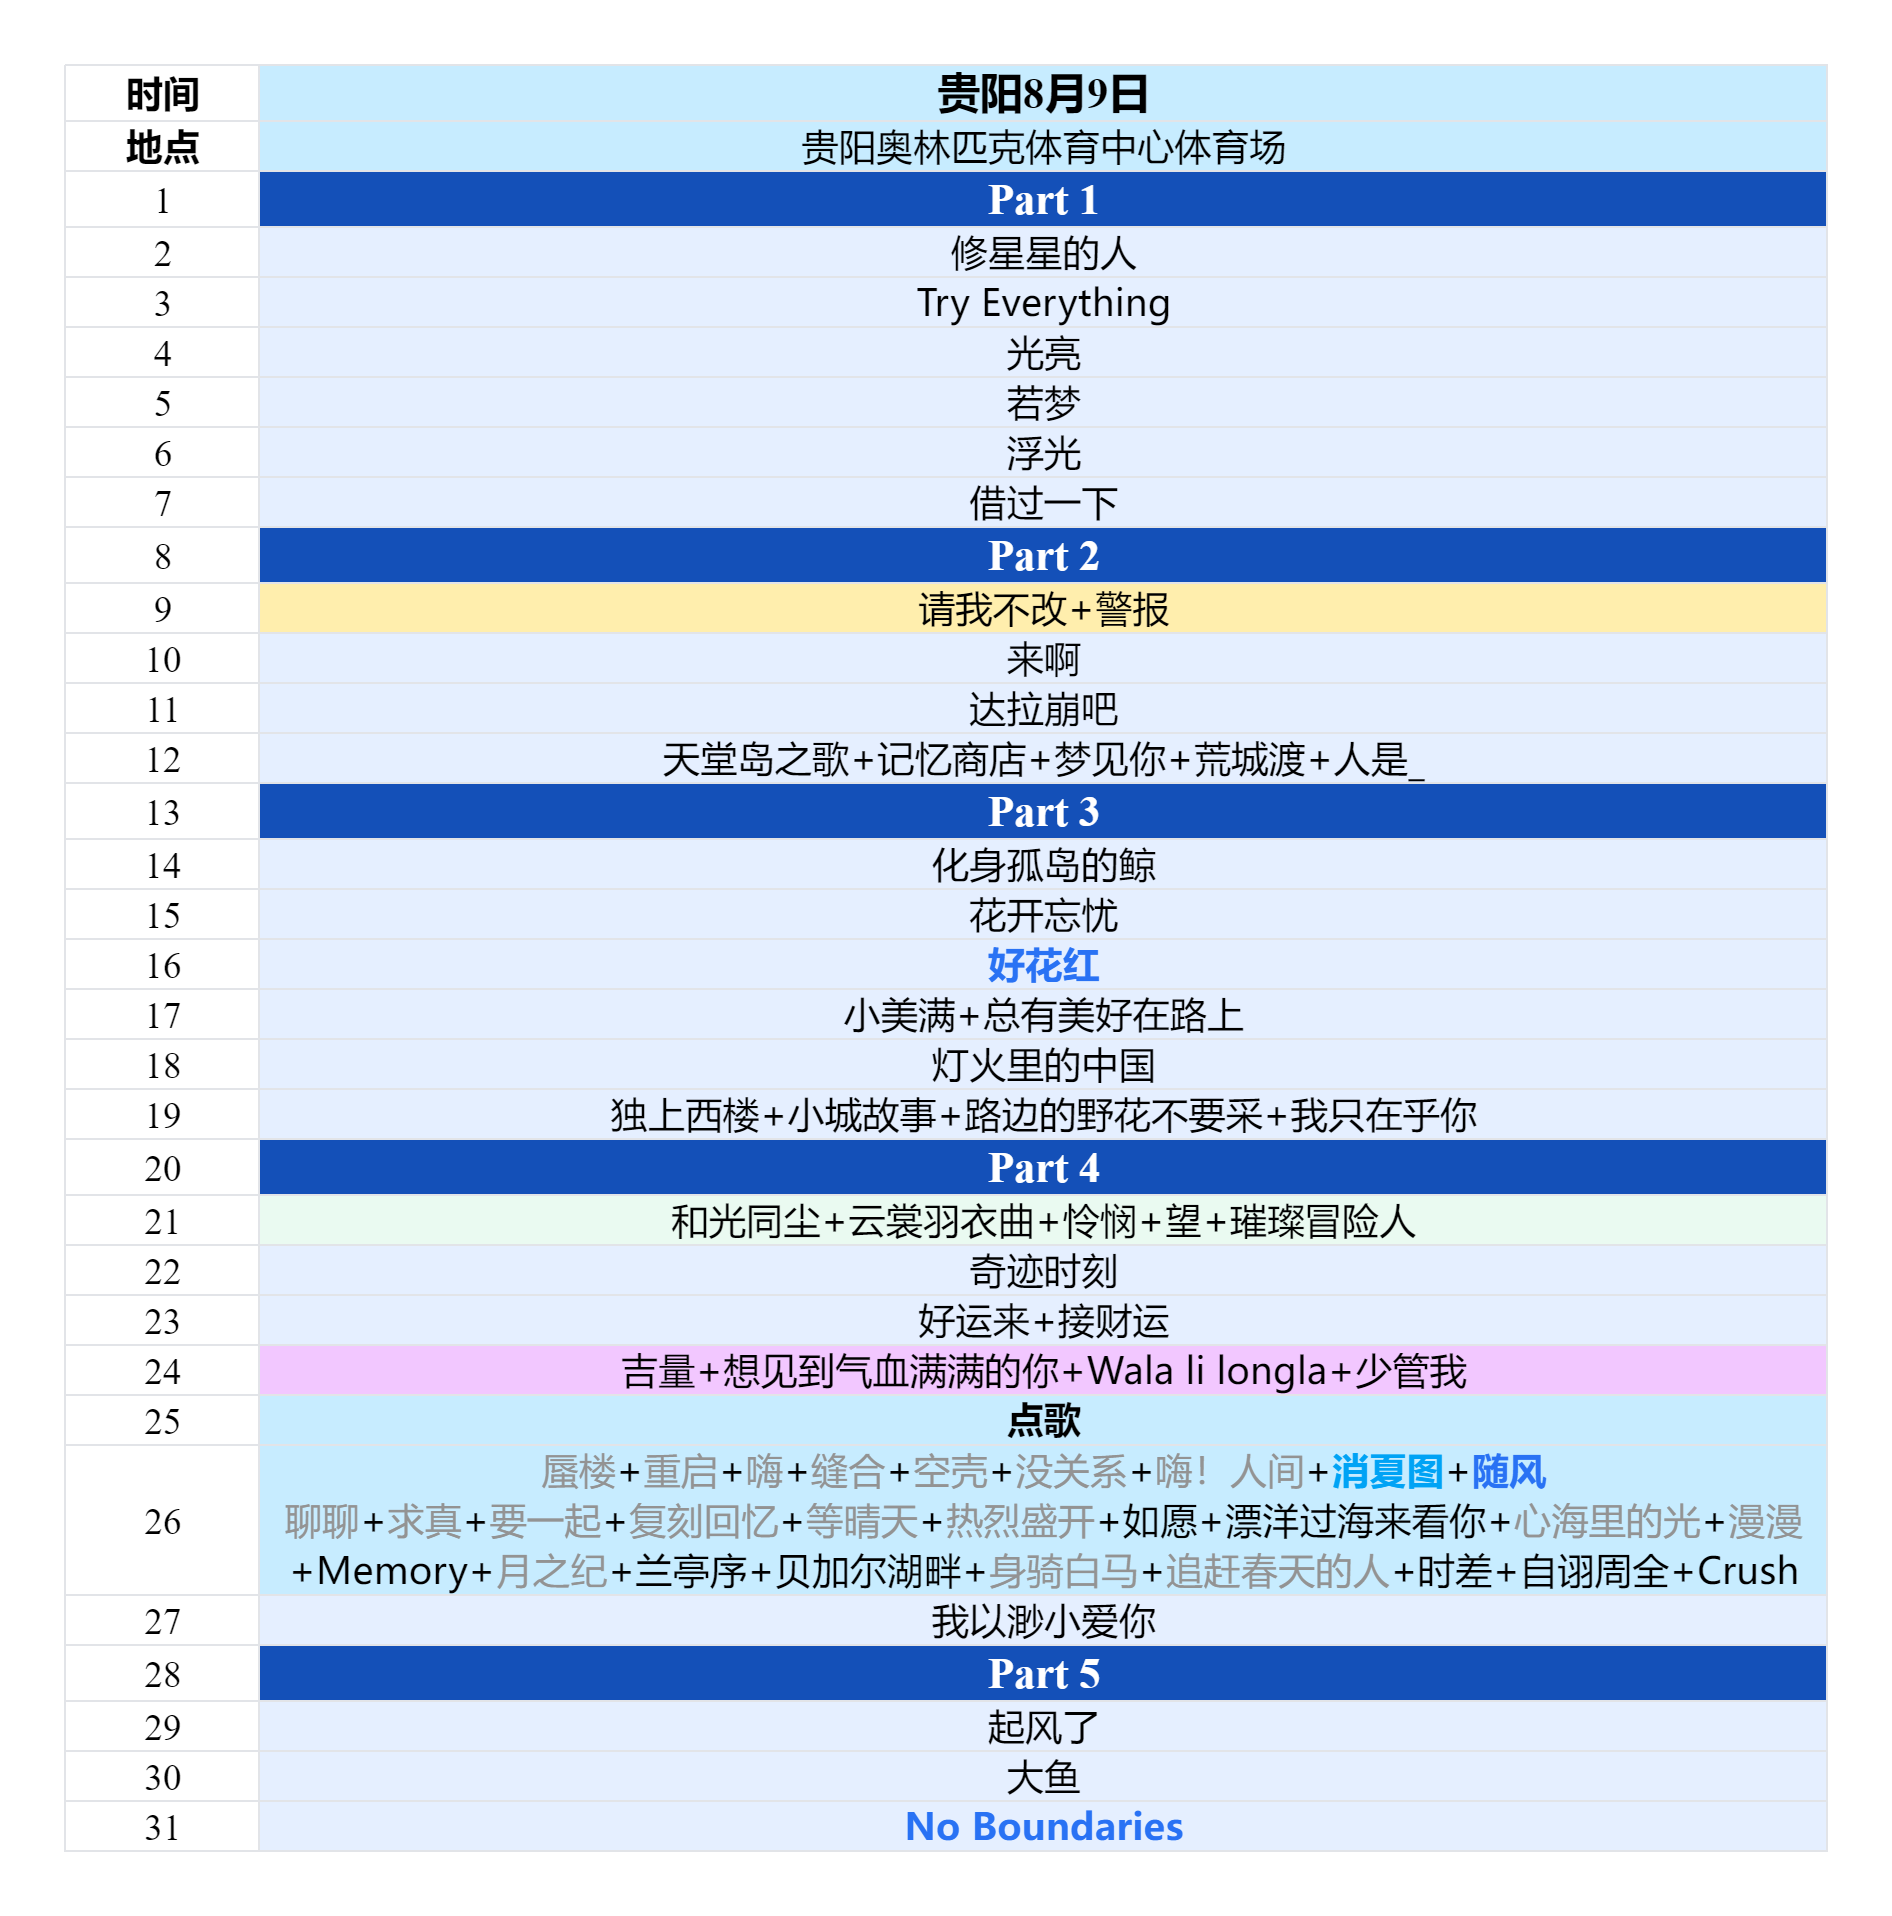
\includegraphics[width=280pt]{img/playlists/GuiYang-20260809} 

}

\caption{2026周深“深深的”巡回演唱会2026.08.09贵阳场歌单}\label{fig:unnamed-chunk-36}
\end{figure}

\newpage

\section{Part1}\label{GuiYang-20260809-part1}

\hyperref[opening-vcr]{🎥【\textbf{开场VCR}】}

\hyperref[xiu-xing-xing-de-ren]{🎵【\textbf{修星星的人}】}

\hyperref[try-everything]{🎵【\textbf{Try Everything}】}

\hyperref[silver-linings]{🎵【\textbf{光亮}】}

\hyperref[like-a-dream]{🎵【\textbf{若梦}】}

\hyperref[floating-light]{🎵【\textbf{浮光}】}

\hyperref[excuse-me]{🎵【\textbf{借过一下}】}

\section{Part2}\label{GuiYang-20260809-part2}

\hyperref[robot-vcr]{🎥【\textbf{机器人VCR}】}

\hyperref[brave-heart]{🎵【\textbf{请我不改}】}

\hyperref[jing-bao]{🎵【\textbf{警报}】}

\hyperref[lai-a]{🎵【\textbf{来啊}】}

\hyperref[dalabengba]{🎵【\textbf{达拉崩吧}】}

\hyperref[haven-song]{🎵【\textbf{天堂岛之歌}】}

\hyperref[the-memory-store]{🎵【\textbf{记忆商店}】}

\hyperref[meng-jian-ni]{🎵【\textbf{梦见你}】}

\hyperref[huang-cheng-du]{🎵【\textbf{荒城渡}】}

\hyperref[Humans_are_]{🎵【\textbf{人是\_}】}

\section{Part3}\label{GuiYang-20260809-part3}

\hyperref[music-animations-vcr]{🎥【\textbf{音乐动画VCR}】}

\hyperref[The-whale-who-became-an-island]{🎵【\textbf{化身孤岛的鲸}】}

\hyperref[Blossoms-that-forget-sorrow]{🎵【\textbf{花开忘忧}】}

\hyperref[hao-hua-hong]{🎵【\textbf{好花红}】}

\hyperref[simple-bliss]{🎵【\textbf{小美满}】}

\hyperref[zong-you-mei-hao-zai-lu-shang]{🎵【\textbf{总有美好在路上}】}

\hyperref[deng-huo-li-de-zhong-guo]{🎵【\textbf{灯火里的中国}】}

🎵【\textbf{邓丽君组曲}】

\hyperref[du-shang-xi-lou]{🎵【\textbf{独上西楼}】}

\hyperref[xiao-cheng-gu-shi]{🎵【\textbf{小城故事}】}

\hyperref[donot-pick-the-roadside-flowers]{🎵【\textbf{路边的野花不要采}】}

\hyperref[I-only-care-about-you]{🎵【\textbf{我只在乎你}】}

\section{Part4}\label{GuiYang-20260809-part4}

\hyperref[mask-vcr]{🎥【\textbf{面具VCR}】}

\hyperref[stay-with-light]{🎵【\textbf{和光同尘}】}

\hyperref[Song-of-the-cloud-dress]{🎵【\textbf{云裳羽衣曲}】}

\hyperref[lian-min]{🎵【\textbf{怜悯}】}

\hyperref[Expectation]{🎵【\textbf{望}】}

\hyperref[adventurers]{🎵【\textbf{璀璨冒险人}】}

\hyperref[miracle-moment]{🎵【\textbf{奇迹时刻}】}

\hyperref[good-fortune-comes]{🎵【\textbf{好运来}】}

\hyperref[jie-cai-yun]{🎵【\textbf{接财运}】}

\hyperref[ji-liang]{🎵【\textbf{吉量}】}

\hyperref[xiang-jian-dao-qi-xue-man-man-de-ni]{🎵【\textbf{想见到气血满满的你}】}

\hyperref[wala-li-longla]{🎵【\textbf{Wala li longla}】}

\hyperref[watch-ur-manners]{🎵【\textbf{少管我}】}

【\textbf{点歌环节}】

\hyperref[sui-feng]{🎵【\textbf{随风}】}

\hyperref[xiao-xia-tu]{🎵【\textbf{消夏图}】}

\hyperref[loving-you-in-my-humble-way]{🎵【\textbf{我以渺小爱你}】}

\section{Part5}\label{GuiYang-20260809-part5}

\hyperref[exchange-diaries-vcr]{🎥【\textbf{交换日记VCR}】}

\hyperref[the-wind-rises]{🎵【\textbf{起风了}】}

\hyperref[big-fish]{🎵【\textbf{大鱼}】}

\hyperref[no-boundaries]{🎵【\textbf{No Boundaries}】}

\chapter{2026.08.22济南场 (WIP)}\label{JiNan-20260822}

\begin{quote}
\begin{flushright}------周深\end{flushright}
\end{quote}

\begin{figure}

{\centering 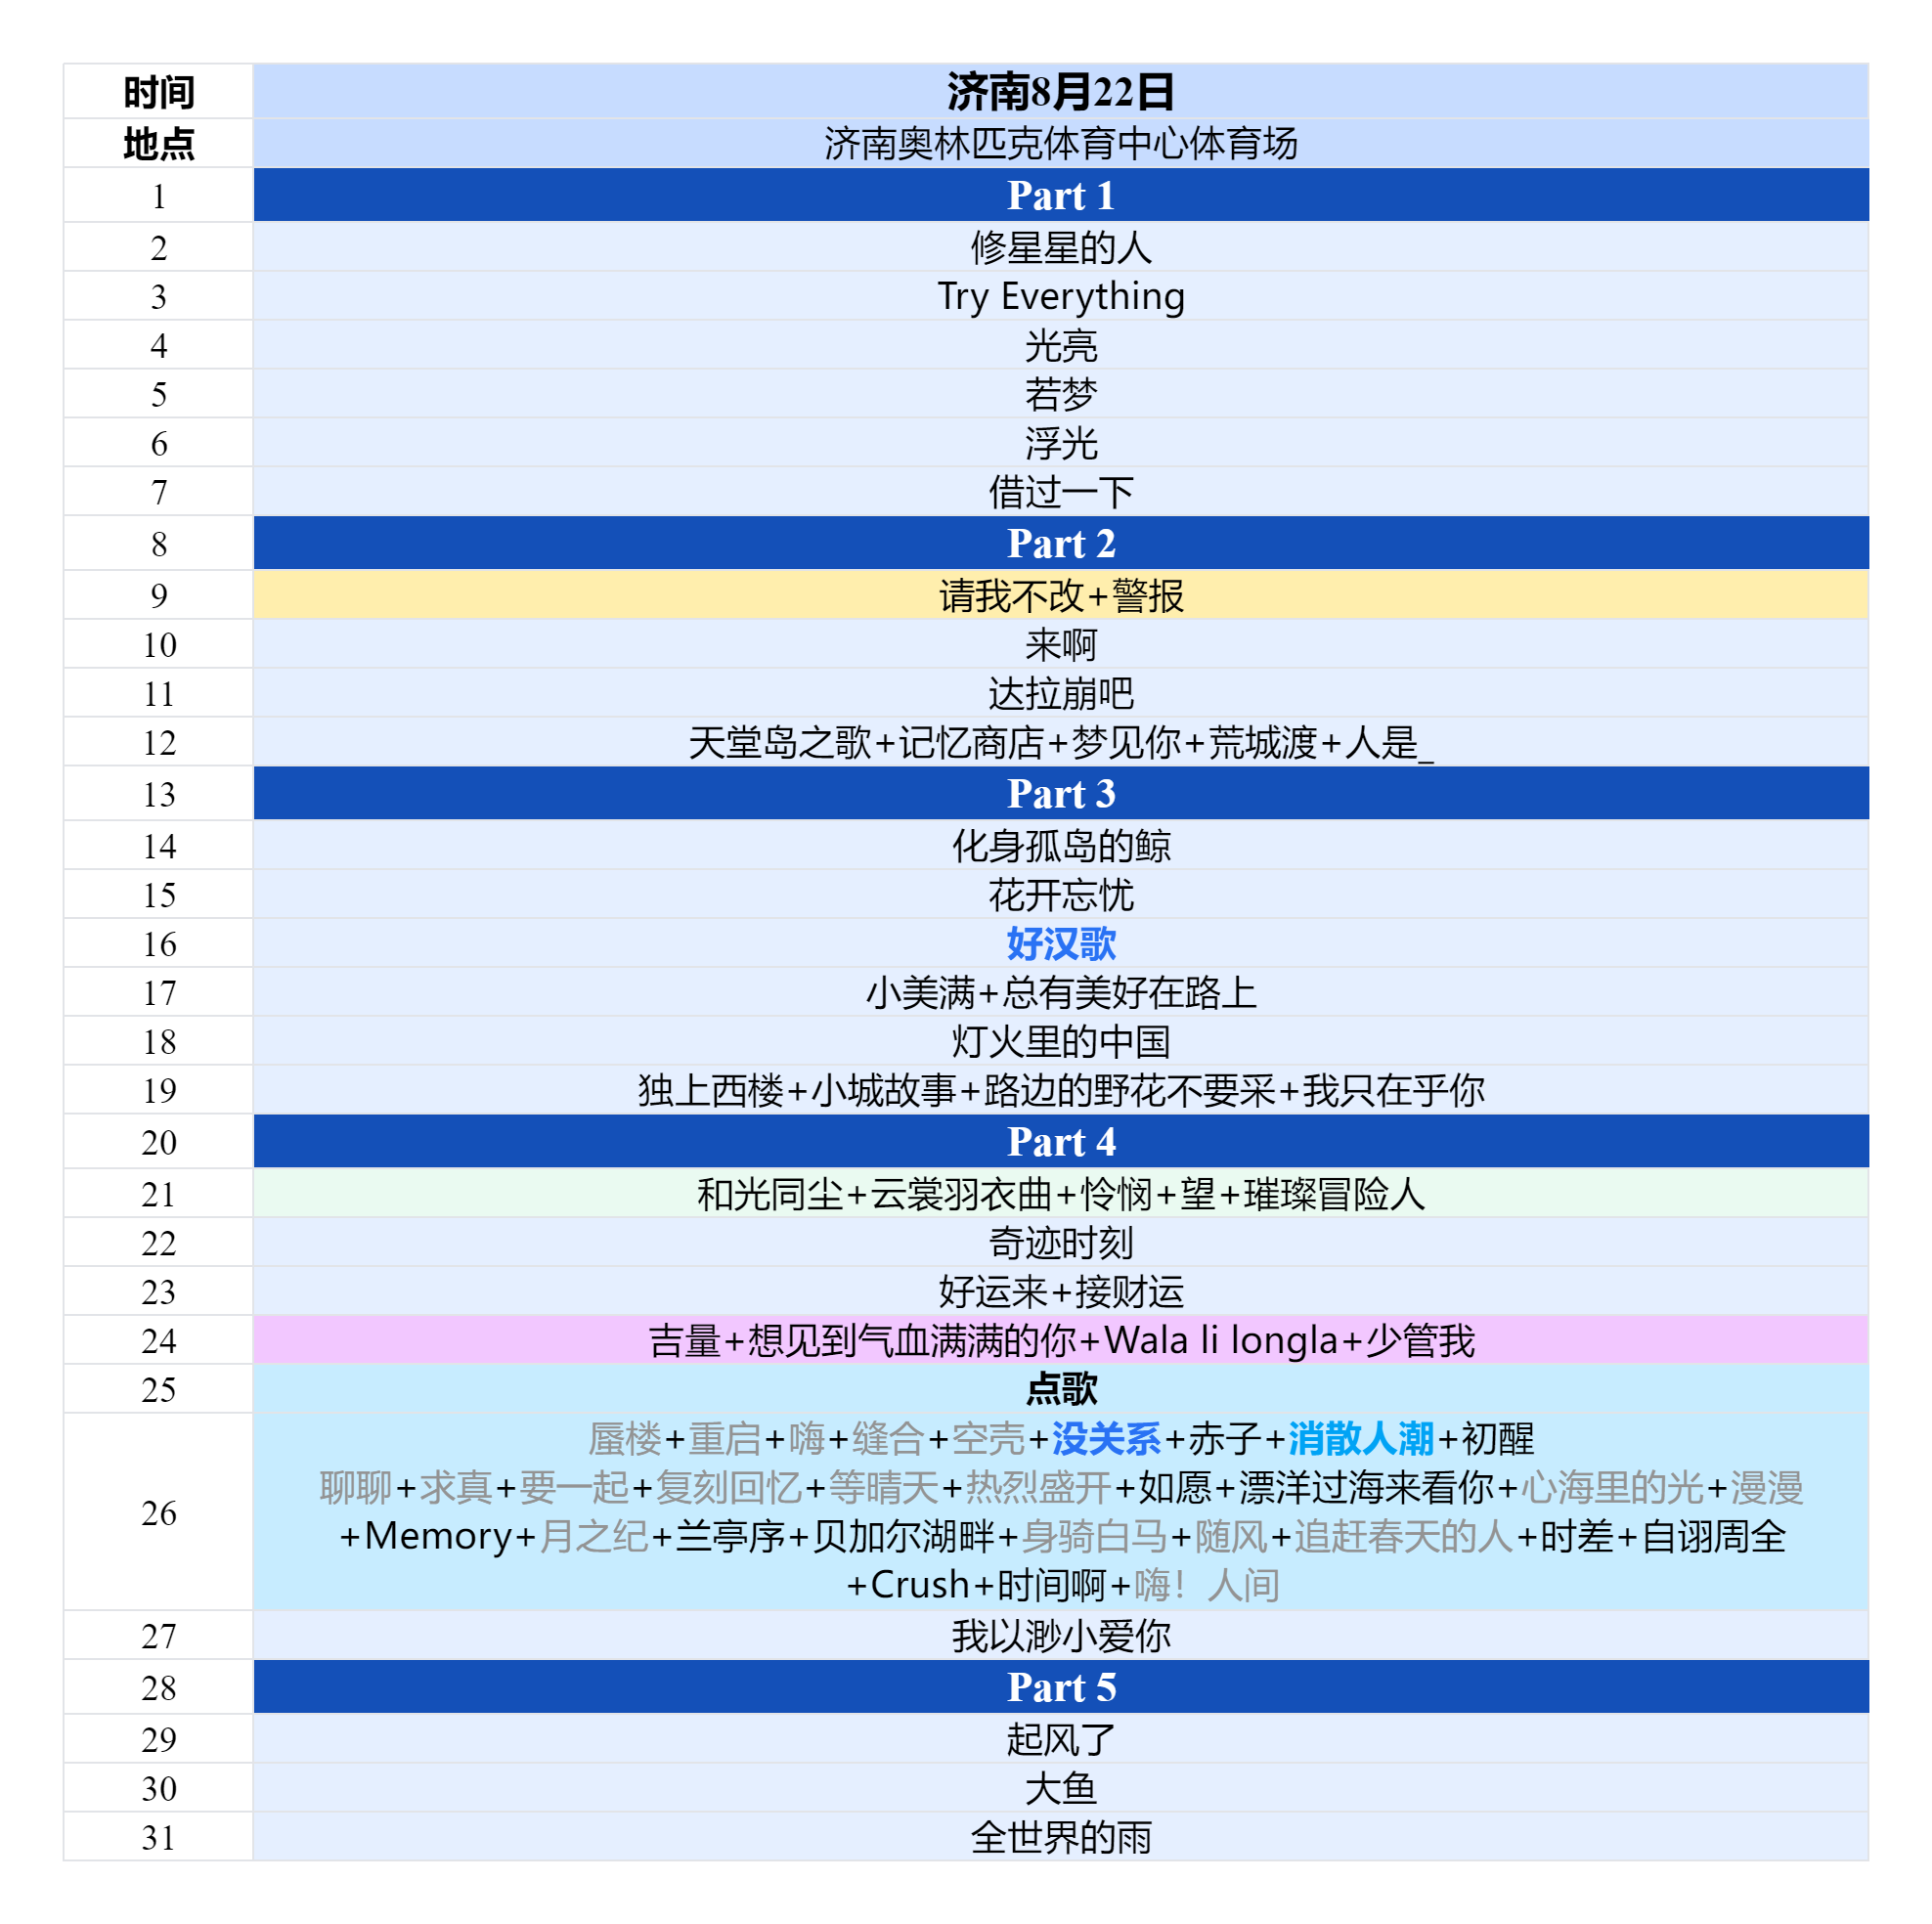
\includegraphics[width=280pt]{img/playlists/JiNan-20260822} 

}

\caption{2026周深“深深的”巡回演唱会2026.08.22济南场歌单}\label{fig:unnamed-chunk-38}
\end{figure}

\newpage

\section{Part1}\label{JiNan-20260822-part1}

\hyperref[opening-vcr]{🎥【\textbf{开场VCR}】}

\hyperref[xiu-xing-xing-de-ren]{🎵【\textbf{修星星的人}】}

\hyperref[try-everything]{🎵【\textbf{Try Everything}】}

\hyperref[silver-linings]{🎵【\textbf{光亮}】}

\hyperref[like-a-dream]{🎵【\textbf{若梦}】}

\hyperref[floating-light]{🎵【\textbf{浮光}】}

\hyperref[excuse-me]{🎵【\textbf{借过一下}】}

\section{Part2}\label{JiNan-20260822-part2}

\hyperref[robot-vcr]{🎥【\textbf{机器人VCR}】}

\hyperref[brave-heart]{🎵【\textbf{请我不改}】}

\hyperref[jing-bao]{🎵【\textbf{警报}】}

\hyperref[lai-a]{🎵【\textbf{来啊}】}

\hyperref[dalabengba]{🎵【\textbf{达拉崩吧}】}

\hyperref[haven-song]{🎵【\textbf{天堂岛之歌}】}

\hyperref[the-memory-store]{🎵【\textbf{记忆商店}】}

\hyperref[meng-jian-ni]{🎵【\textbf{梦见你}】}

\hyperref[huang-cheng-du]{🎵【\textbf{荒城渡}】}

\hyperref[Humans_are_]{🎵【\textbf{人是\_}】}

\section{Part3}\label{JiNan-20260822-part3}

\hyperref[music-animations-vcr]{🎥【\textbf{音乐动画VCR}】}

\hyperref[The-whale-who-became-an-island]{🎵【\textbf{化身孤岛的鲸}】}

\hyperref[Blossoms-that-forget-sorrow]{🎵【\textbf{花开忘忧}】}

\hyperref[hao-han-ge]{🎵【\textbf{好汉歌}】}

\hyperref[simple-bliss]{🎵【\textbf{小美满}】}

\hyperref[zong-you-mei-hao-zai-lu-shang]{🎵【\textbf{总有美好在路上}】}

\hyperref[deng-huo-li-de-zhong-guo]{🎵【\textbf{灯火里的中国}】}

🎵【\textbf{邓丽君组曲}】

\hyperref[du-shang-xi-lou]{🎵【\textbf{独上西楼}】}

\hyperref[xiao-cheng-gu-shi]{🎵【\textbf{小城故事}】}

\hyperref[donot-pick-the-roadside-flowers]{🎵【\textbf{路边的野花不要采}】}

\hyperref[I-only-care-about-you]{🎵【\textbf{我只在乎你}】}

\section{Part4}\label{JiNan-20260822-part4}

\hyperref[mask-vcr]{🎥【\textbf{面具VCR}】}

\hyperref[stay-with-light]{🎵【\textbf{和光同尘}】}

\hyperref[Song-of-the-cloud-dress]{🎵【\textbf{云裳羽衣曲}】}

\hyperref[lian-min]{🎵【\textbf{怜悯}】}

\hyperref[Expectation]{🎵【\textbf{望}】}

\hyperref[adventurers]{🎵【\textbf{璀璨冒险人}】}

\hyperref[miracle-moment]{🎵【\textbf{奇迹时刻}】}

\hyperref[good-fortune-comes]{🎵【\textbf{好运来}】}

\hyperref[jie-cai-yun]{🎵【\textbf{接财运}】}

\hyperref[ji-liang]{🎵【\textbf{吉量}】}

\hyperref[xiang-jian-dao-qi-xue-man-man-de-ni]{🎵【\textbf{想见到气血满满的你}】}

\hyperref[wala-li-longla]{🎵【\textbf{Wala li longla}】}

\hyperref[watch-ur-manners]{🎵【\textbf{少管我}】}

【\textbf{点歌环节}】

\hyperref[mei-guan-xi]{🎵【\textbf{没关系}】}

\hyperref[xiao-san-ren-chao]{🎵【\textbf{消散人潮}】}

\hyperref[loving-you-in-my-humble-way]{🎵【\textbf{我以渺小爱你}】}

\section{Part5}\label{JiNan-20260822-part5}

\hyperref[exchange-diaries-vcr]{🎥【\textbf{交换日记VCR}】}

\hyperref[the-wind-rises]{🎵【\textbf{起风了}】}

\hyperref[big-fish]{🎵【\textbf{大鱼}】}

\hyperref[quan-shi-jie-de-yu]{🎵【\textbf{全世界的雨}】}

\chapter{2026.08.23济南场 (WIP)}\label{JiNan-20260823}

\begin{quote}
\begin{flushright}------周深\end{flushright}
\end{quote}

\begin{figure}

{\centering 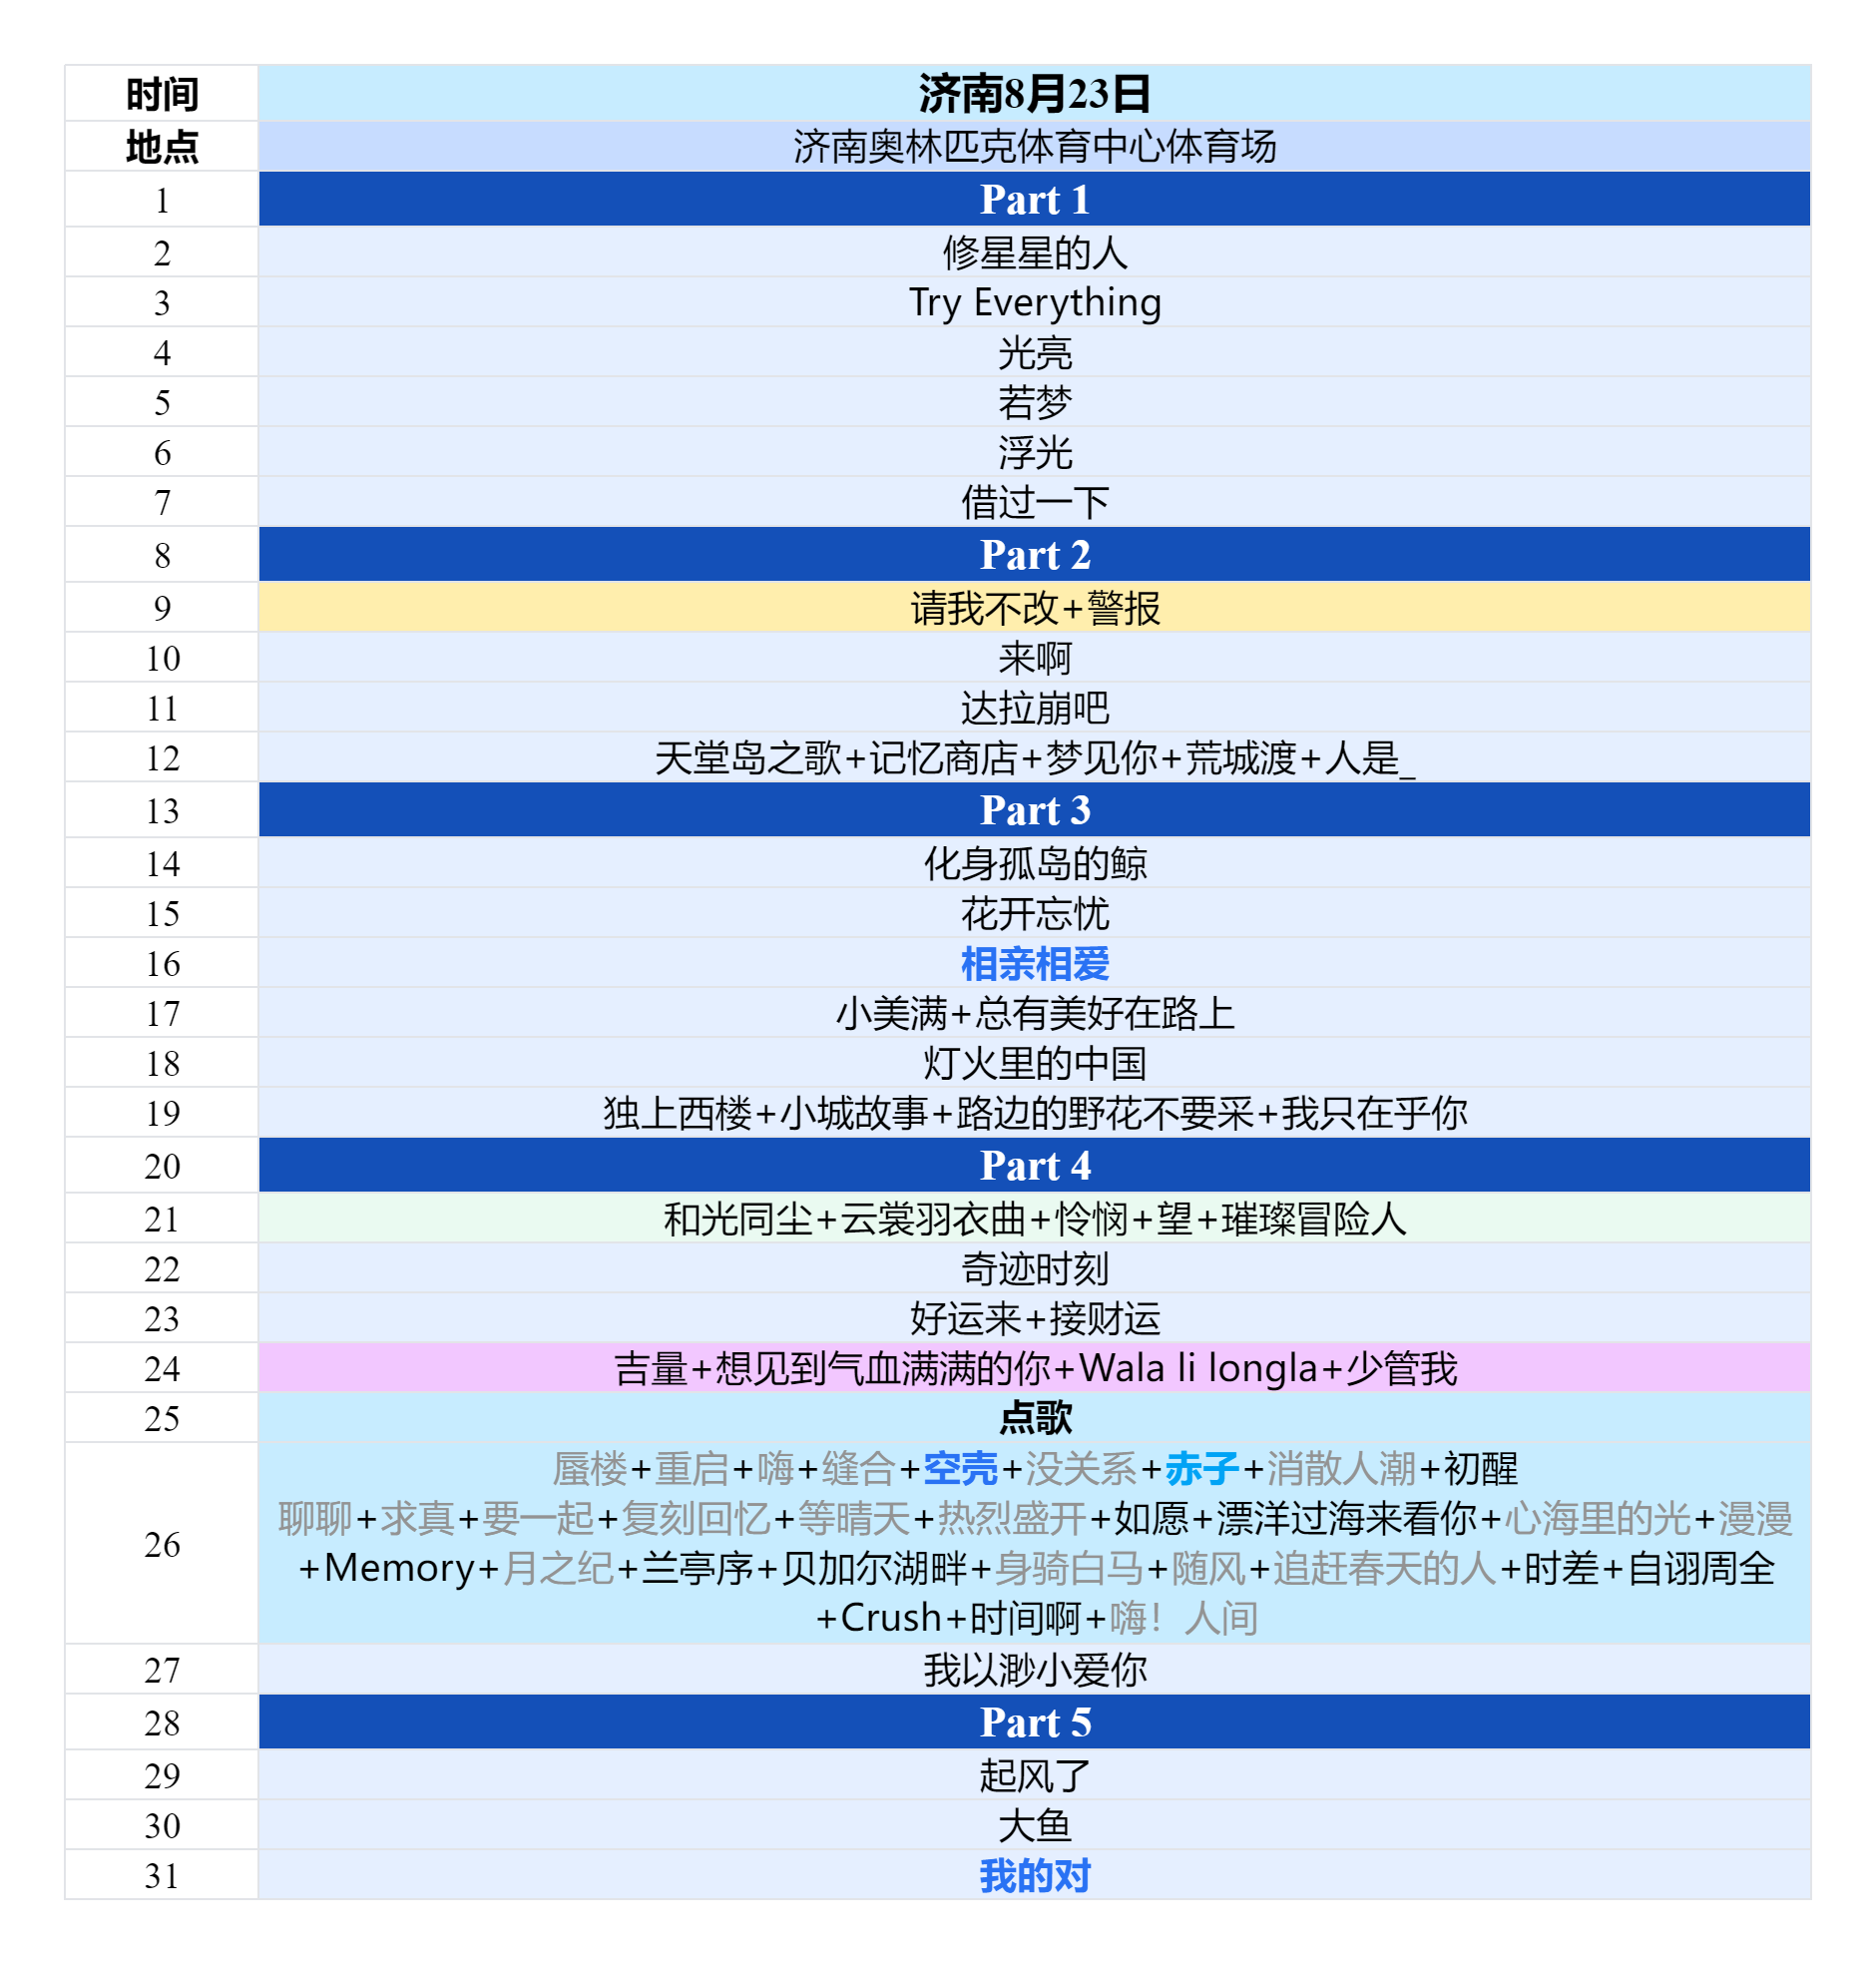
\includegraphics[width=280pt]{img/playlists/JiNan-20260823} 

}

\caption{2026周深“深深的”巡回演唱会2026.08.23济南场歌单}\label{fig:unnamed-chunk-40}
\end{figure}

\newpage

\section{Part1}\label{JiNan-20260823-part1}

\hyperref[opening-vcr]{🎥【\textbf{开场VCR}】}

\hyperref[xiu-xing-xing-de-ren]{🎵【\textbf{修星星的人}】}

\hyperref[try-everything]{🎵【\textbf{Try Everything}】}

\hyperref[silver-linings]{🎵【\textbf{光亮}】}

\hyperref[like-a-dream]{🎵【\textbf{若梦}】}

\hyperref[floating-light]{🎵【\textbf{浮光}】}

\hyperref[excuse-me]{🎵【\textbf{借过一下}】}

\section{Part2}\label{JiNan-20260823-part2}

\hyperref[robot-vcr]{🎥【\textbf{机器人VCR}】}

\hyperref[brave-heart]{🎵【\textbf{请我不改}】}

\hyperref[jing-bao]{🎵【\textbf{警报}】}

\hyperref[lai-a]{🎵【\textbf{来啊}】}

\hyperref[dalabengba]{🎵【\textbf{达拉崩吧}】}

\hyperref[haven-song]{🎵【\textbf{天堂岛之歌}】}

\hyperref[the-memory-store]{🎵【\textbf{记忆商店}】}

\hyperref[meng-jian-ni]{🎵【\textbf{梦见你}】}

\hyperref[huang-cheng-du]{🎵【\textbf{荒城渡}】}

\hyperref[Humans_are_]{🎵【\textbf{人是\_}】}

\section{Part3}\label{JiNan-20260823-part3}

\hyperref[music-animations-vcr]{🎥【\textbf{音乐动画VCR}】}

\hyperref[The-whale-who-became-an-island]{🎵【\textbf{化身孤岛的鲸}】}

\hyperref[Blossoms-that-forget-sorrow]{🎵【\textbf{花开忘忧}】}

\hyperref[xiang-qin-xiang-ai]{🎵【\textbf{相亲相爱}】}

\hyperref[simple-bliss]{🎵【\textbf{小美满}】}

\hyperref[zong-you-mei-hao-zai-lu-shang]{🎵【\textbf{总有美好在路上}】}

\hyperref[deng-huo-li-de-zhong-guo]{🎵【\textbf{灯火里的中国}】}

🎵【\textbf{邓丽君组曲}】

\hyperref[du-shang-xi-lou]{🎵【\textbf{独上西楼}】}

\hyperref[xiao-cheng-gu-shi]{🎵【\textbf{小城故事}】}

\hyperref[donot-pick-the-roadside-flowers]{🎵【\textbf{路边的野花不要采}】}

\hyperref[I-only-care-about-you]{🎵【\textbf{我只在乎你}】}

\section{Part4}\label{JiNan-20260823-part4}

\hyperref[mask-vcr]{🎥【\textbf{面具VCR}】}

\hyperref[stay-with-light]{🎵【\textbf{和光同尘}】}

\hyperref[Song-of-the-cloud-dress]{🎵【\textbf{云裳羽衣曲}】}

\hyperref[lian-min]{🎵【\textbf{怜悯}】}

\hyperref[Expectation]{🎵【\textbf{望}】}

\hyperref[adventurers]{🎵【\textbf{璀璨冒险人}】}

\hyperref[miracle-moment]{🎵【\textbf{奇迹时刻}】}

\hyperref[good-fortune-comes]{🎵【\textbf{好运来}】}

\hyperref[jie-cai-yun]{🎵【\textbf{接财运}】}

\hyperref[ji-liang]{🎵【\textbf{吉量}】}

\hyperref[xiang-jian-dao-qi-xue-man-man-de-ni]{🎵【\textbf{想见到气血满满的你}】}

\hyperref[wala-li-longla]{🎵【\textbf{Wala li longla}】}

\hyperref[watch-ur-manners]{🎵【\textbf{少管我}】}

【\textbf{点歌环节}】

\hyperref[kong-ke]{🎵【\textbf{空壳}】}

\hyperref[chi-zi]{🎵【\textbf{赤子}】}

\hyperref[loving-you-in-my-humble-way]{🎵【\textbf{我以渺小爱你}】}

\section{Part5}\label{JiNan-20260823-part5}

\hyperref[exchange-diaries-vcr]{🎥【\textbf{交换日记VCR}】}

\hyperref[the-wind-rises]{🎵【\textbf{起风了}】}

\hyperref[big-fish]{🎵【\textbf{大鱼}】}

\hyperref[wo-de-dui]{🎵【\textbf{我的对}】}

\chapter{2026.09.12台州场 (WIP)}\label{TaiZhou-20260912}

\begin{quote}
\begin{flushright}------周深\end{flushright}
\end{quote}

\begin{figure}

{\centering 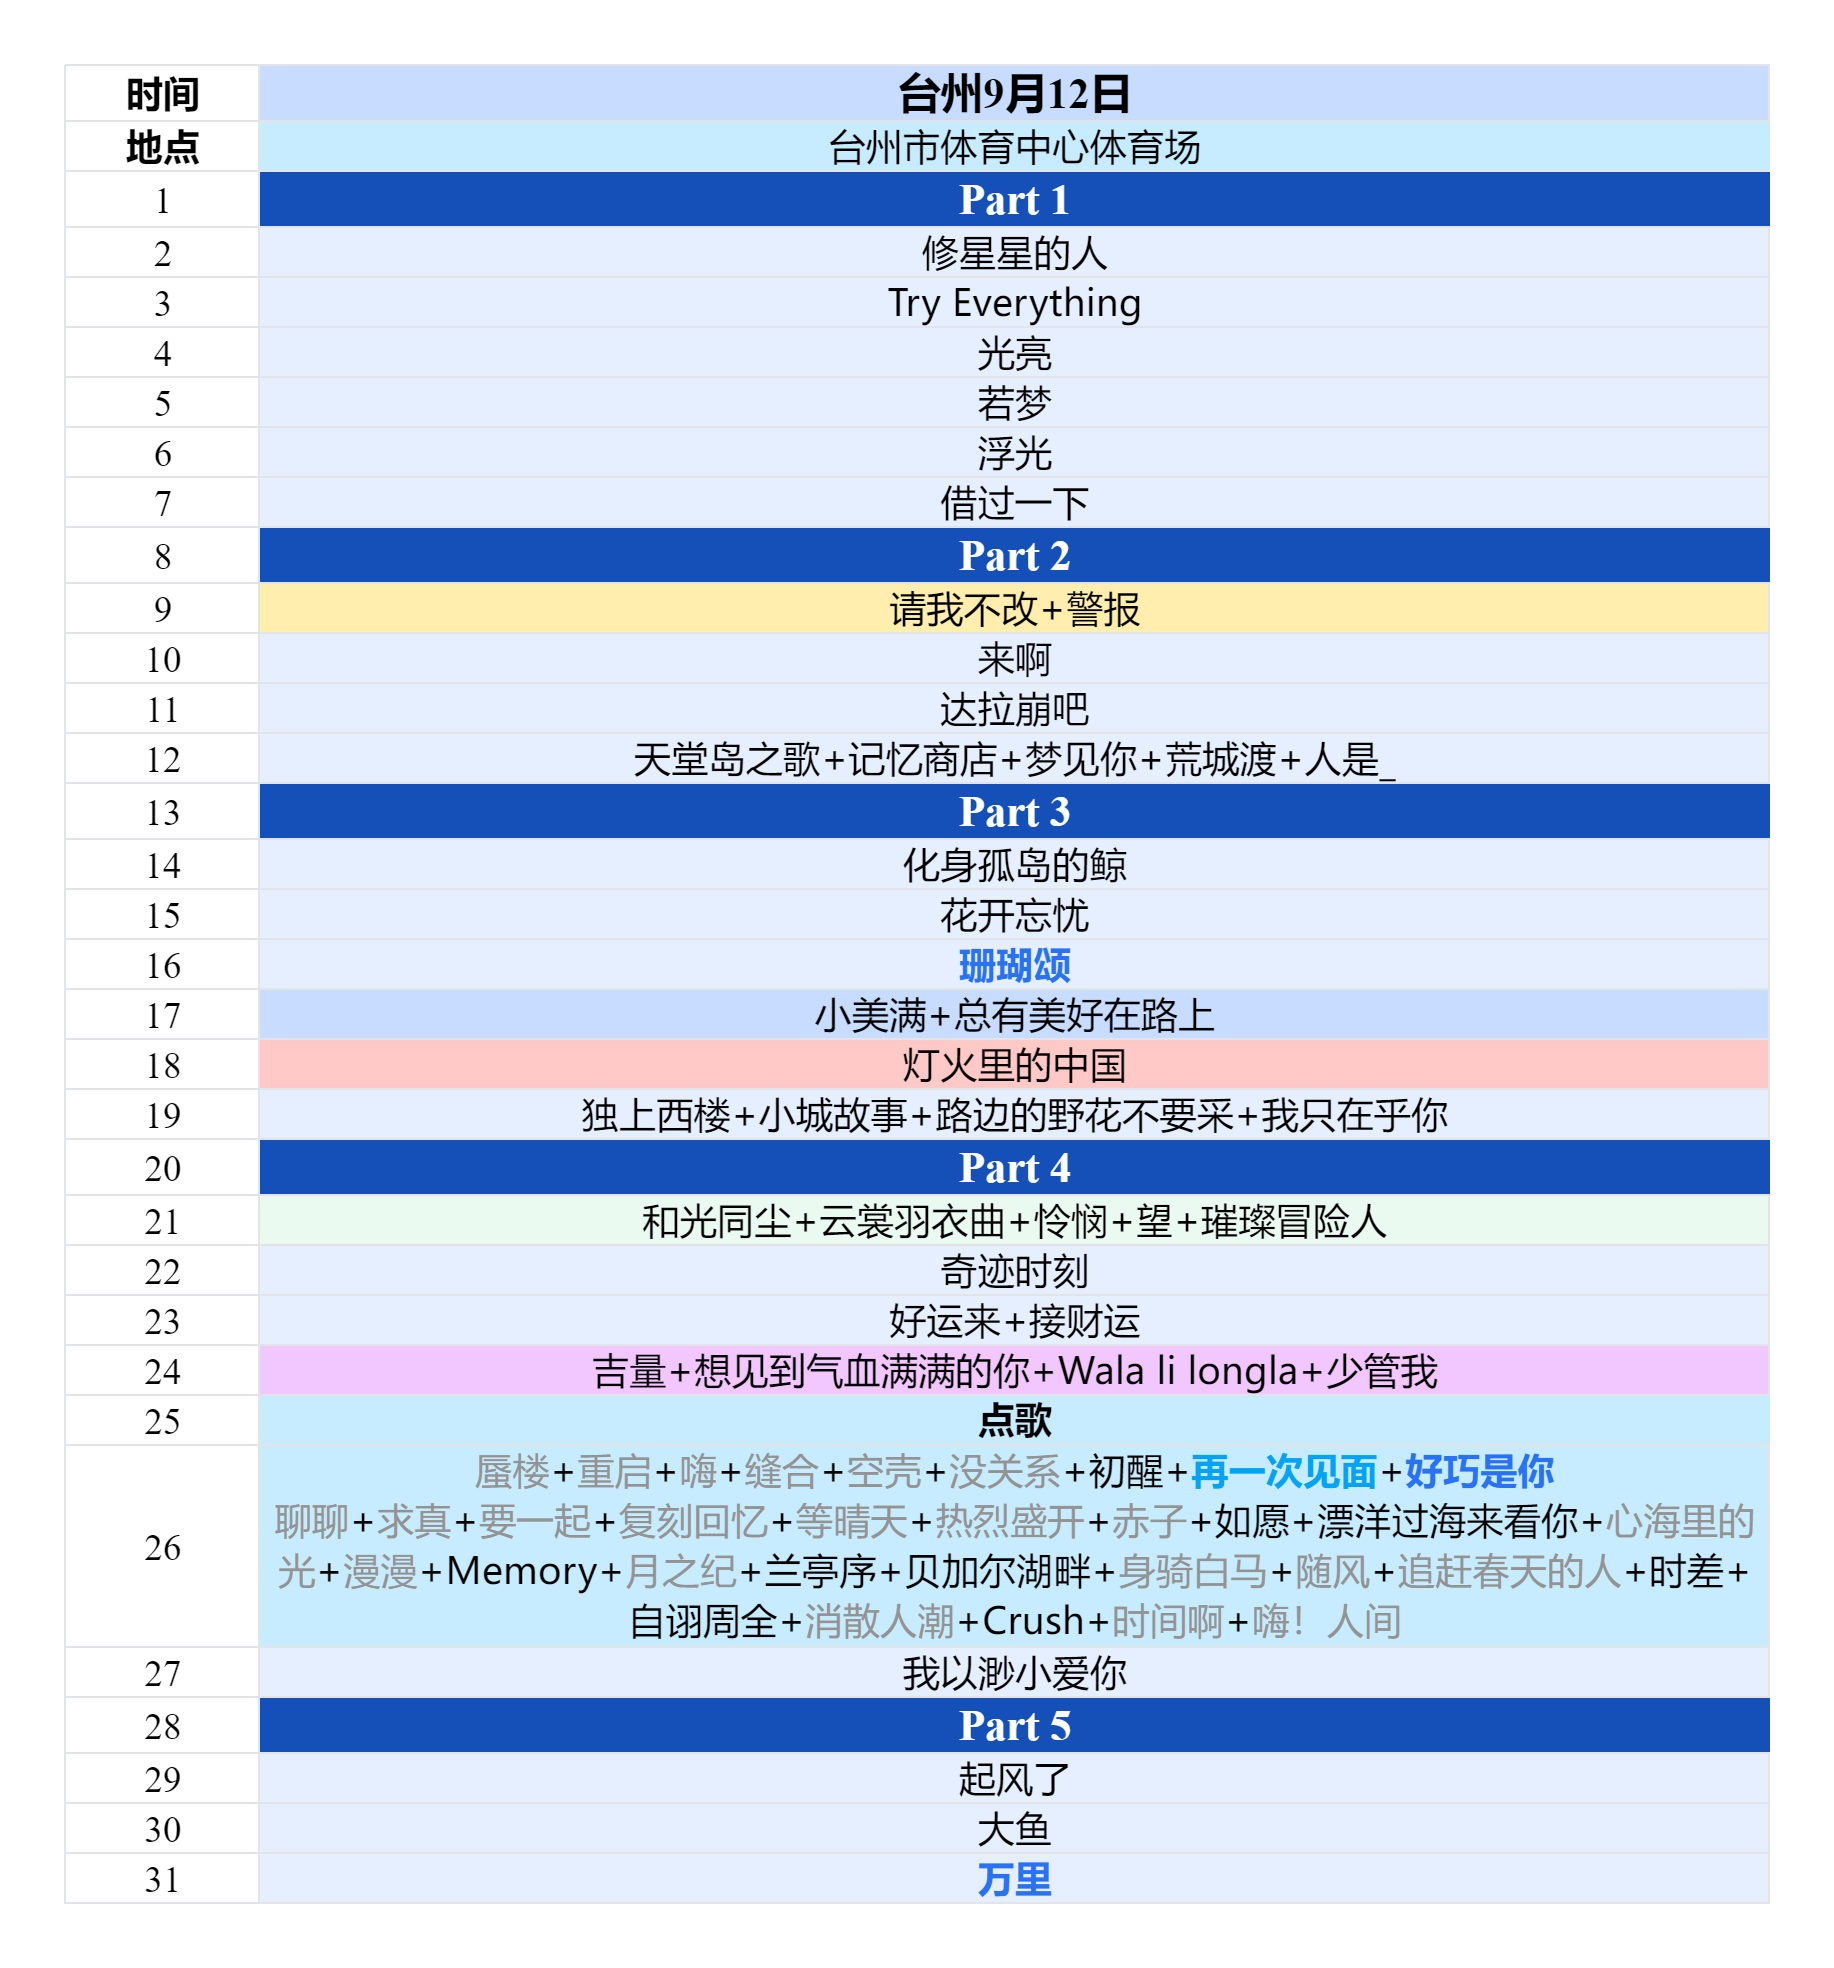
\includegraphics[width=280pt]{img/playlists/TaiZhou-20260912} 

}

\caption{2026周深“深深的”巡回演唱会2026.09.12台州场歌单}\label{fig:unnamed-chunk-42}
\end{figure}

\newpage

\section{Part1}\label{TaiZhou-20260912-part1}

\hyperref[opening-vcr]{🎥【\textbf{开场VCR}】}

\hyperref[xiu-xing-xing-de-ren]{🎵【\textbf{修星星的人}】}

\hyperref[try-everything]{🎵【\textbf{Try Everything}】}

\hyperref[silver-linings]{🎵【\textbf{光亮}】}

\hyperref[like-a-dream]{🎵【\textbf{若梦}】}

\hyperref[floating-light]{🎵【\textbf{浮光}】}

\hyperref[excuse-me]{🎵【\textbf{借过一下}】}

\section{Part2}\label{TaiZhou-20260912-part2}

\hyperref[robot-vcr]{🎥【\textbf{机器人VCR}】}

\hyperref[brave-heart]{🎵【\textbf{请我不改}】}

\hyperref[jing-bao]{🎵【\textbf{警报}】}

\hyperref[lai-a]{🎵【\textbf{来啊}】}

\hyperref[dalabengba]{🎵【\textbf{达拉崩吧}】}

\hyperref[haven-song]{🎵【\textbf{天堂岛之歌}】}

\hyperref[the-memory-store]{🎵【\textbf{记忆商店}】}

\hyperref[meng-jian-ni]{🎵【\textbf{梦见你}】}

\hyperref[huang-cheng-du]{🎵【\textbf{荒城渡}】}

\hyperref[Humans_are_]{🎵【\textbf{人是\_}】}

\section{Part3}\label{TaiZhou-20260912-part3}

\hyperref[music-animations-vcr]{🎥【\textbf{音乐动画VCR}】}

\hyperref[The-whale-who-became-an-island]{🎵【\textbf{化身孤岛的鲸}】}

\hyperref[Blossoms-that-forget-sorrow]{🎵【\textbf{花开忘忧}】}

\hyperref[shan-hu-song]{🎵【\textbf{珊瑚颂}】}

\hyperref[simple-bliss]{🎵【\textbf{小美满}】}

\hyperref[zong-you-mei-hao-zai-lu-shang]{🎵【\textbf{总有美好在路上}】}

\hyperref[deng-huo-li-de-zhong-guo]{🎵【\textbf{灯火里的中国}】}

🎵【\textbf{邓丽君组曲}】

\hyperref[du-shang-xi-lou]{🎵【\textbf{独上西楼}】}

\hyperref[xiao-cheng-gu-shi]{🎵【\textbf{小城故事}】}

\hyperref[donot-pick-the-roadside-flowers]{🎵【\textbf{路边的野花不要采}】}

\hyperref[I-only-care-about-you]{🎵【\textbf{我只在乎你}】}

\section{Part4}\label{TaiZhou-20260912-part4}

\hyperref[mask-vcr]{🎥【\textbf{面具VCR}】}

\hyperref[stay-with-light]{🎵【\textbf{和光同尘}】}

\hyperref[Song-of-the-cloud-dress]{🎵【\textbf{云裳羽衣曲}】}

\hyperref[lian-min]{🎵【\textbf{怜悯}】}

\hyperref[Expectation]{🎵【\textbf{望}】}

\hyperref[adventurers]{🎵【\textbf{璀璨冒险人}】}

\hyperref[miracle-moment]{🎵【\textbf{奇迹时刻}】}

\hyperref[good-fortune-comes]{🎵【\textbf{好运来}】}

\hyperref[jie-cai-yun]{🎵【\textbf{接财运}】}

\hyperref[ji-liang]{🎵【\textbf{吉量}】}

\hyperref[xiang-jian-dao-qi-xue-man-man-de-ni]{🎵【\textbf{想见到气血满满的你}】}

\hyperref[wala-li-longla]{🎵【\textbf{Wala li longla}】}

\hyperref[watch-ur-manners]{🎵【\textbf{少管我}】}

【\textbf{点歌环节}】

\hyperref[hao-qiao-shi-ni]{🎵【\textbf{好巧是你}】}

\hyperref[zai-yi-ci-jian-mian]{🎵【\textbf{再一次见面}】}

\hyperref[loving-you-in-my-humble-way]{🎵【\textbf{我以渺小爱你}】}

\section{Part5}\label{TaiZhou-20260912-part5}

\hyperref[exchange-diaries-vcr]{🎥【\textbf{交换日记VCR}】}

\hyperref[the-wind-rises]{🎵【\textbf{起风了}】}

\hyperref[big-fish]{🎵【\textbf{大鱼}】}

\hyperref[wan-li]{🎵【\textbf{万里}】}

\chapter{2026.09.13台州场 (WIP)}\label{TaiZhou-20260913}

\begin{quote}
\begin{flushright}------周深\end{flushright}
\end{quote}

\begin{figure}

{\centering 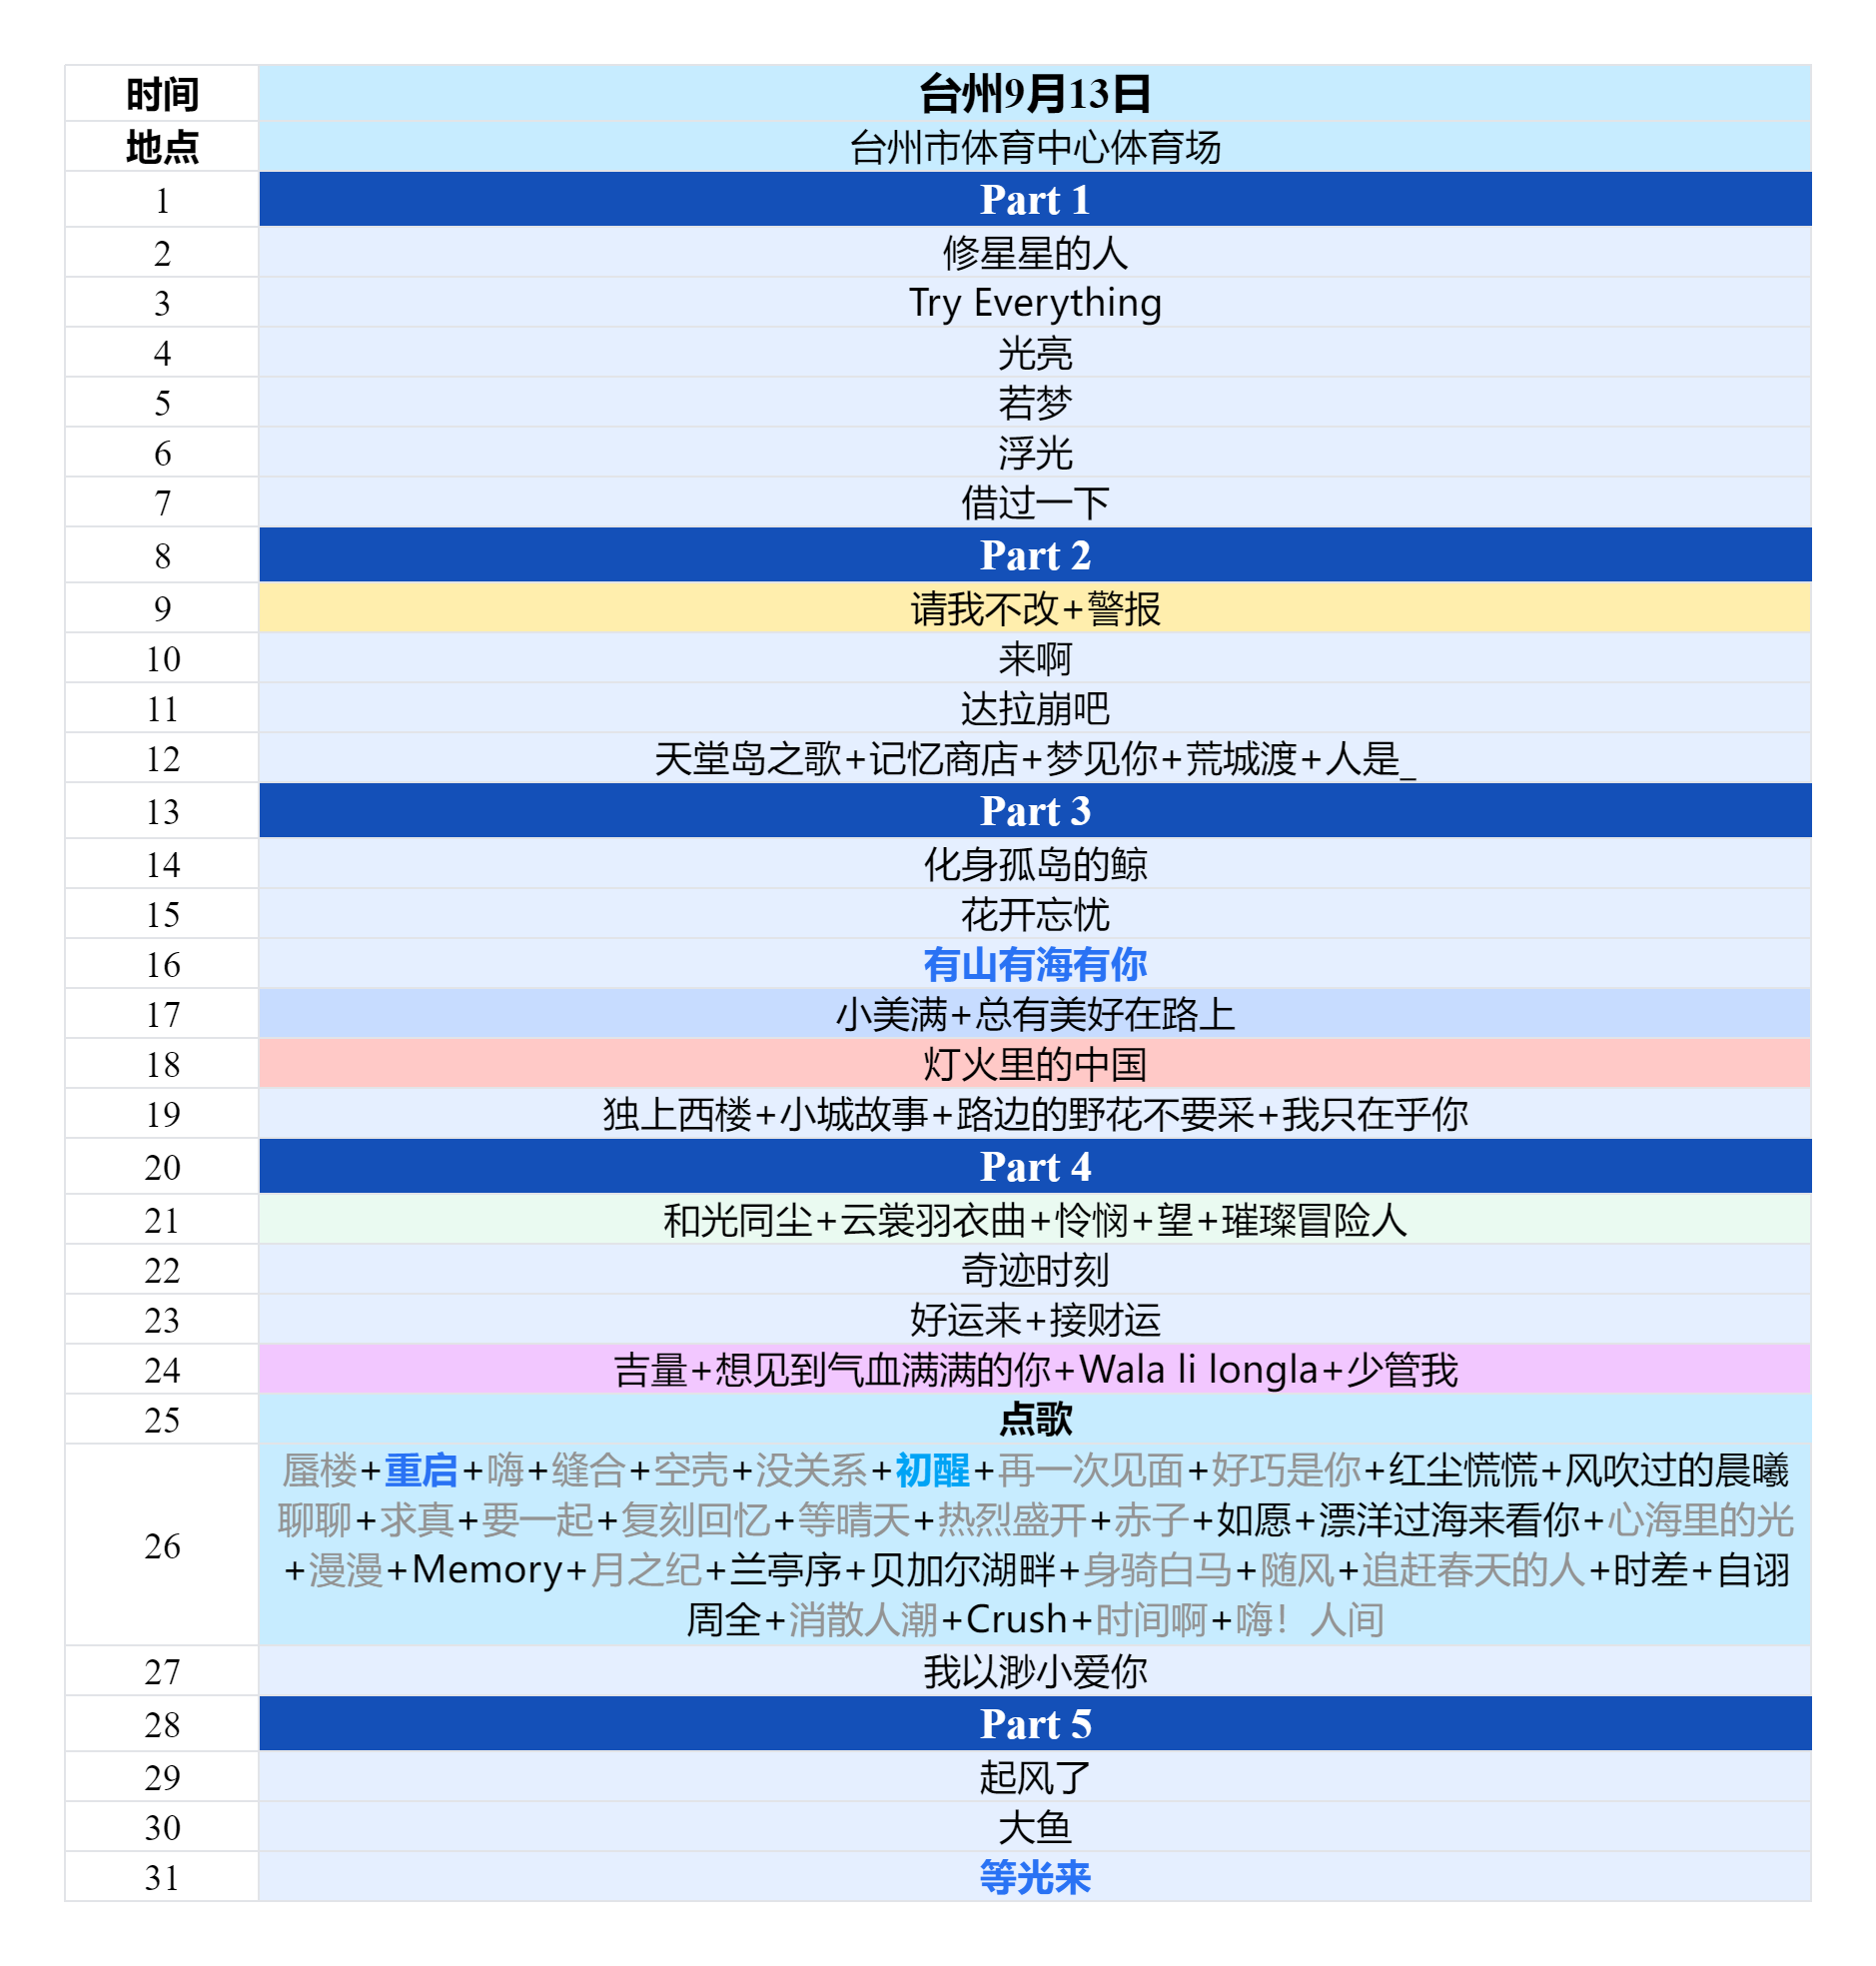
\includegraphics[width=280pt]{img/playlists/TaiZhou-20260913} 

}

\caption{2026周深“深深的”巡回演唱会2026.09.13台州场歌单}\label{fig:unnamed-chunk-44}
\end{figure}

\newpage

\section{Part1}\label{TaiZhou-20260913-part1}

\hyperref[opening-vcr]{🎥【\textbf{开场VCR}】}

\hyperref[xiu-xing-xing-de-ren]{🎵【\textbf{修星星的人}】}

\hyperref[try-everything]{🎵【\textbf{Try Everything}】}

\hyperref[silver-linings]{🎵【\textbf{光亮}】}

\hyperref[like-a-dream]{🎵【\textbf{若梦}】}

\hyperref[floating-light]{🎵【\textbf{浮光}】}

\hyperref[excuse-me]{🎵【\textbf{借过一下}】}

\section{Part2}\label{TaiZhou-20260913-part2}

\hyperref[robot-vcr]{🎥【\textbf{机器人VCR}】}

\hyperref[brave-heart]{🎵【\textbf{请我不改}】}

\hyperref[jing-bao]{🎵【\textbf{警报}】}

\hyperref[lai-a]{🎵【\textbf{来啊}】}

\hyperref[dalabengba]{🎵【\textbf{达拉崩吧}】}

\hyperref[haven-song]{🎵【\textbf{天堂岛之歌}】}

\hyperref[the-memory-store]{🎵【\textbf{记忆商店}】}

\hyperref[meng-jian-ni]{🎵【\textbf{梦见你}】}

\hyperref[huang-cheng-du]{🎵【\textbf{荒城渡}】}

\hyperref[Humans_are_]{🎵【\textbf{人是\_}】}

\section{Part3}\label{TaiZhou-20260913-part3}

\hyperref[music-animations-vcr]{🎥【\textbf{音乐动画VCR}】}

\hyperref[The-whale-who-became-an-island]{🎵【\textbf{化身孤岛的鲸}】}

\hyperref[Blossoms-that-forget-sorrow]{🎵【\textbf{花开忘忧}】}

\hyperref[you-shan-you-hai-you-ni]{🎵【\textbf{有山有海有你}】}

\hyperref[simple-bliss]{🎵【\textbf{小美满}】}

\hyperref[zong-you-mei-hao-zai-lu-shang]{🎵【\textbf{总有美好在路上}】}

\hyperref[deng-huo-li-de-zhong-guo]{🎵【\textbf{灯火里的中国}】}

🎵【\textbf{邓丽君组曲}】

\hyperref[du-shang-xi-lou]{🎵【\textbf{独上西楼}】}

\hyperref[xiao-cheng-gu-shi]{🎵【\textbf{小城故事}】}

\hyperref[donot-pick-the-roadside-flowers]{🎵【\textbf{路边的野花不要采}】}

\hyperref[I-only-care-about-you]{🎵【\textbf{我只在乎你}】}

\section{Part4}\label{TaiZhou-20260913-part4}

\hyperref[mask-vcr]{🎥【\textbf{面具VCR}】}

\hyperref[stay-with-light]{🎵【\textbf{和光同尘}】}

\hyperref[Song-of-the-cloud-dress]{🎵【\textbf{云裳羽衣曲}】}

\hyperref[lian-min]{🎵【\textbf{怜悯}】}

\hyperref[Expectation]{🎵【\textbf{望}】}

\hyperref[adventurers]{🎵【\textbf{璀璨冒险人}】}

\hyperref[miracle-moment]{🎵【\textbf{奇迹时刻}】}

\hyperref[good-fortune-comes]{🎵【\textbf{好运来}】}

\hyperref[jie-cai-yun]{🎵【\textbf{接财运}】}

\hyperref[ji-liang]{🎵【\textbf{吉量}】}

\hyperref[xiang-jian-dao-qi-xue-man-man-de-ni]{🎵【\textbf{想见到气血满满的你}】}

\hyperref[wala-li-longla]{🎵【\textbf{Wala li longla}】}

\hyperref[watch-ur-manners]{🎵【\textbf{少管我}】}

【\textbf{点歌环节}】

\hyperref[chong-qi]{🎵【\textbf{重启}】}

\hyperref[chu-xing]{🎵【\textbf{初醒}】}

\hyperref[loving-you-in-my-humble-way]{🎵【\textbf{我以渺小爱你}】}

\section{Part5}\label{TaiZhou-20260913-part5}

\hyperref[exchange-diaries-vcr]{🎥【\textbf{交换日记VCR}】}

\hyperref[the-wind-rises]{🎵【\textbf{起风了}】}

\hyperref[big-fish]{🎵【\textbf{大鱼}】}

\hyperref[deng-guang-lai]{🎵【\textbf{等光来}】}

\chapter{2026.09.25北京场 (WIP)}\label{BeiJing-20260925}

\begin{quote}
``这可是鸟巢啊！朋友们，我们做到了啦！''------周深
\end{quote}

\begin{figure}

{\centering 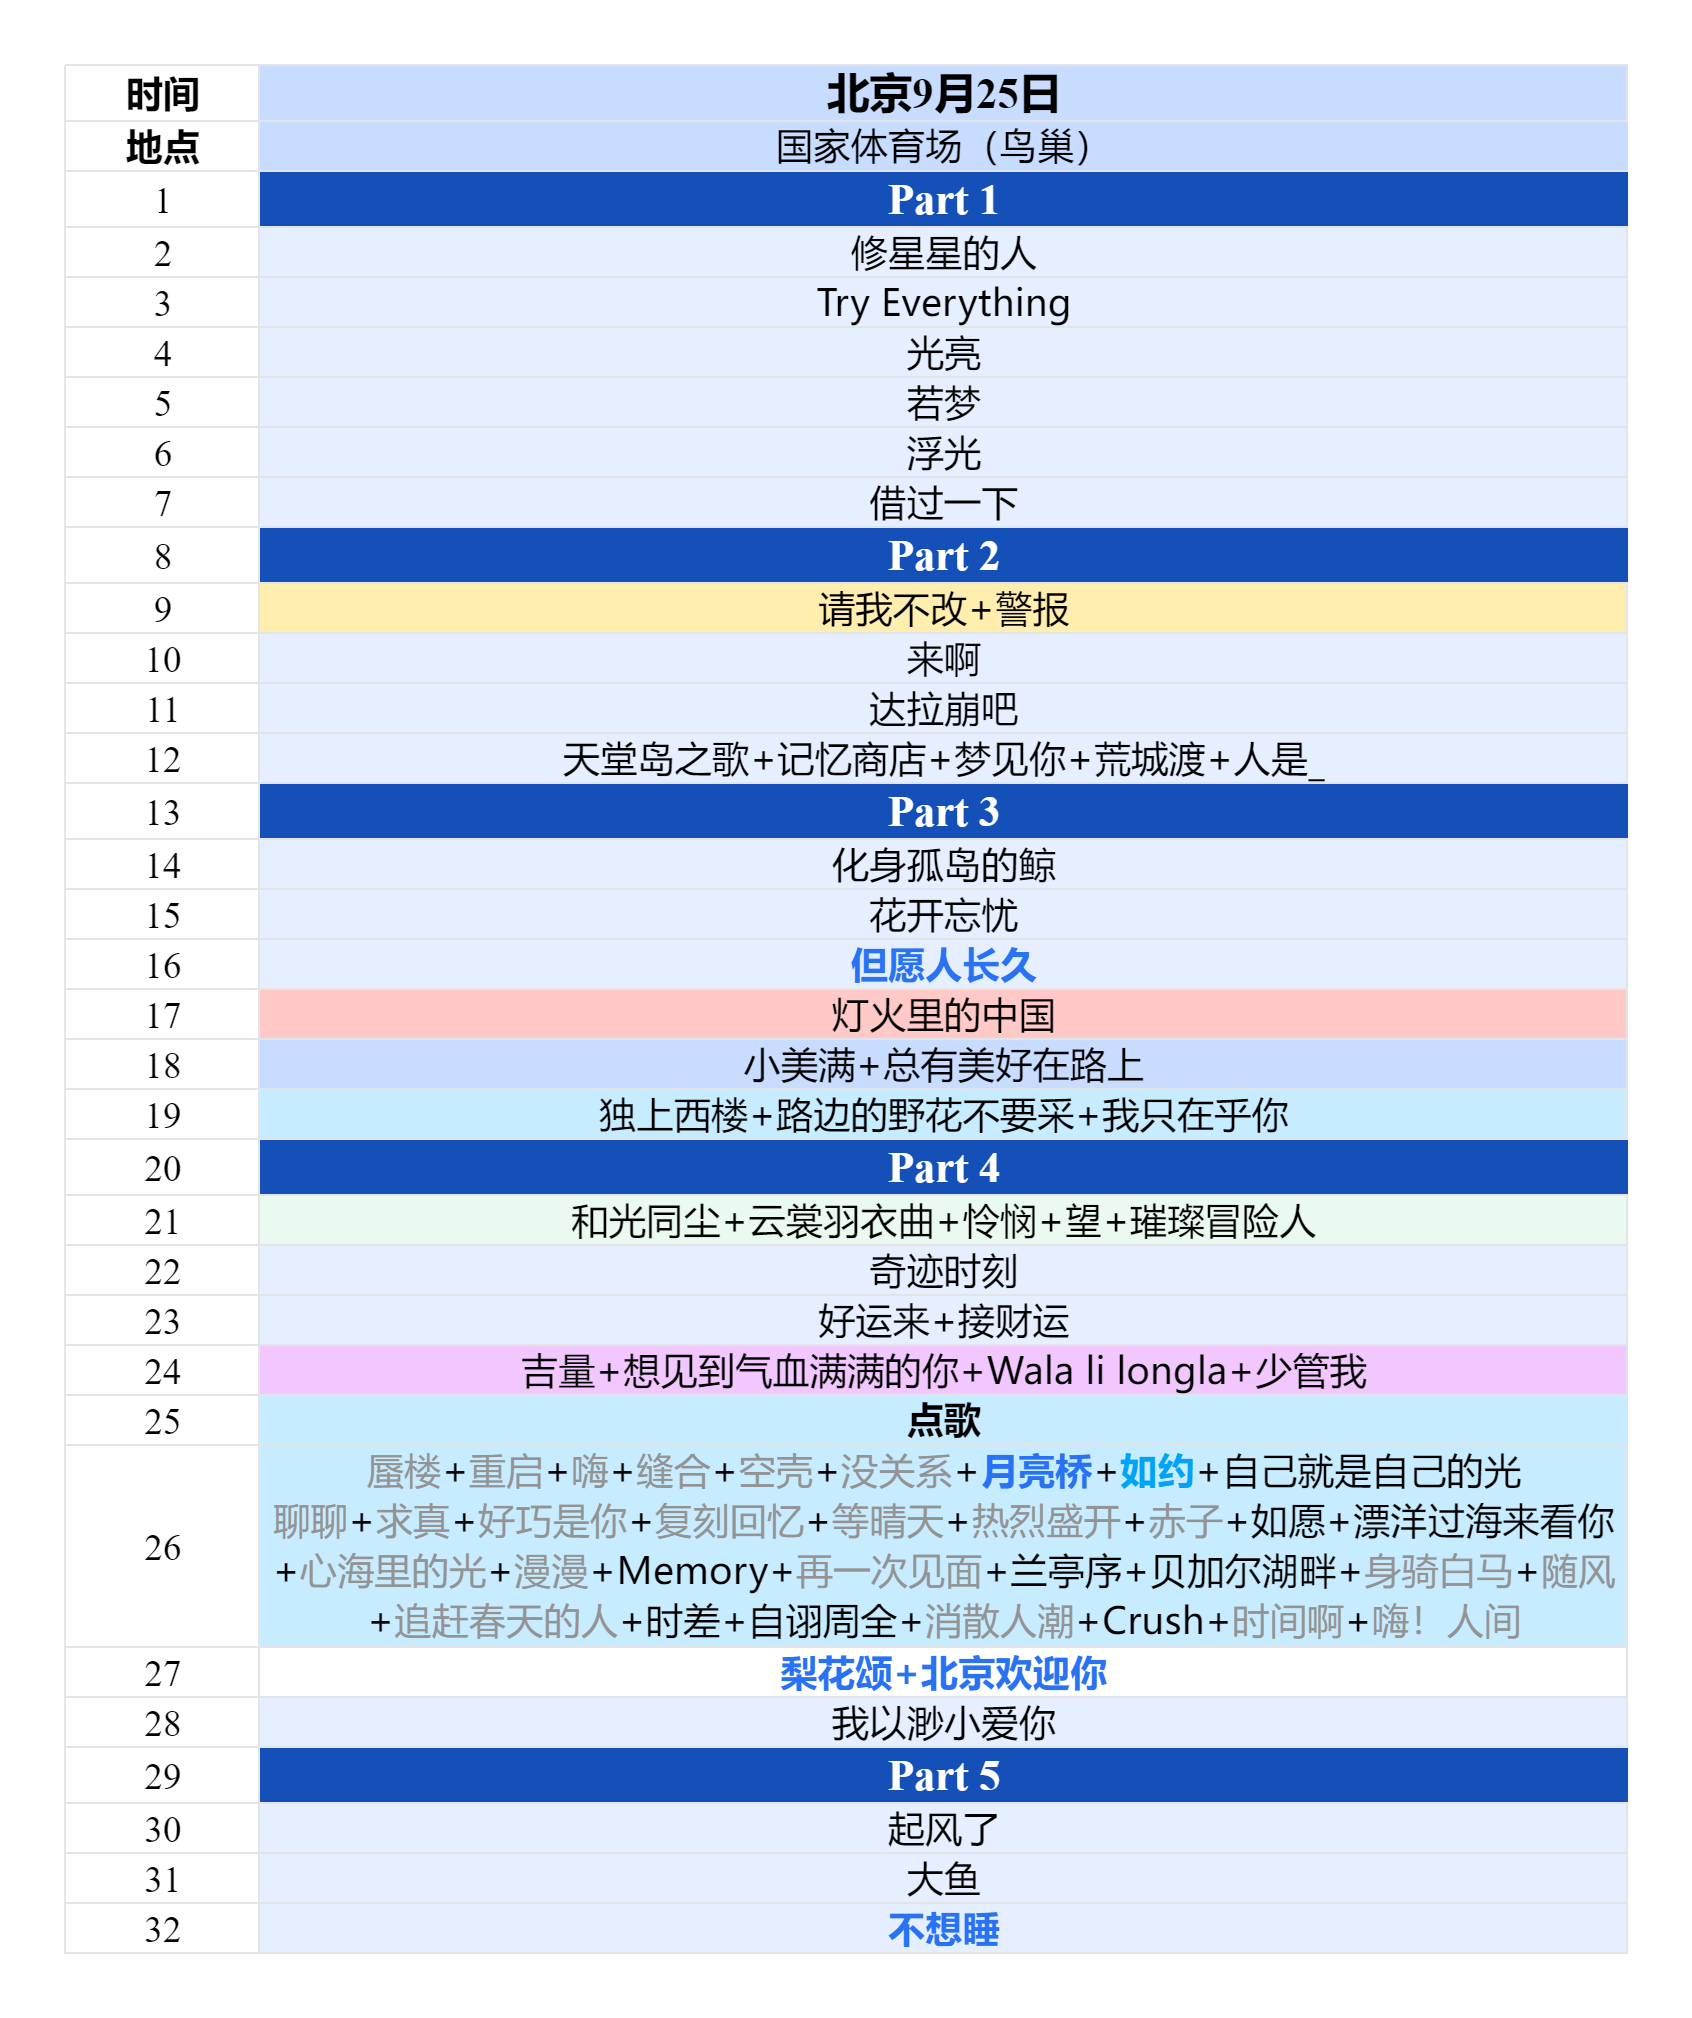
\includegraphics[width=280pt]{img/playlists/BeiJing-20260925} 

}

\caption{2026周深“深深的”巡回演唱会2026.11.07常州场歌单}\label{fig:unnamed-chunk-46}
\end{figure}

\newpage

\section{Part1}\label{BeiJing-20260925-part1}

\hyperref[opening-vcr]{🎥【\textbf{开场VCR}】}（VCR 正文见附录 D。VCR 结束后《修星星的人》前奏直接响起。）

\hyperref[xiu-xing-xing-de-ren]{🎵【\textbf{修星星的人}】}（米：先声合唱：既然这宇宙让我诞生------）（深：是我在故乡的旷野，仰望银河的夏夜；是我在宇宙的风暴，朝着天仓五飘曳；我的孤独我的热烈，源自137亿年前，几粒星尘的蝴蝶；在噬星的幻灭里，为太阳撑一把雨伞；在时间的深海里，给地球道一声晚安〔首句现场听作''是我在无尽的光年''，``给地球''或作''给北京''，待核〕）北京的朋友们你们好吗！（米：好------！）（深：既然这宇宙让我诞生，想必它是要以我为证；我的情感和三十六度的体温，足以暖热即将熄灭的恒星\ldots\ldots 许我以造物的碎屑，重塑文明的边界；许我以渺小的羞怯，挽留物种的毁灭〔第二段主歌现场听作''是我们在破碎后重塑文明的边界，是屋顶渺小的锈迹挽留雾中的归燕''，现场版唱词待核〕）（深：既然这宇宙予我重生，想必它是要让我看懂，我的基因和闪闪发光的记忆，足以照亮所有星际的永恒）（高音吟唱）鸟巢的朋友们你们好吗！（米：好！）

\hyperref[try-everything]{🎵【\textbf{Try Everything}】}既然宇宙让我们诞生，就勇敢地 Try Everything 好不好？（米：好！）（深：I messed up tonight, I lost another fight / I still mess up but I'll just start again\ldots\ldots No I won't leave, I wanna try everything / I wanna try even though I could fail）（深：Oh oh oh oh oh------到你们！）（米：Try everything!）（深：Oh oh oh oh oh------）（米：Try everything!）（深：Oh oh oh oh oh------）（米：Try everything!）（深：Oh oh oh oh oh------）（深：你们好吗？）（深：I won't give up, no I won't give in\ldots\ldots Look how far you've come, you filled your heart with love / Baby you've done enough, take a deep breath\ldots\ldots I'll keep on making those new mistakes / I'll keep on making them every day / Those new mistakes）全场的朋友！（米：Try everything!）再大声！（米：Try everything!）最大声！（米：Try everything!）

\hyperref[silver-linings]{🎵【\textbf{光亮}】}哇！北京的朋友们，你们好吗？（米：好------！）后面的朋友你们好吗？（米：好------！）这边的朋友你们好吗？（米：好------！）哇，我们深深的巡回演唱会终于来到鸟巢了。让我再听一下鸟巢的朋友们的声音，你们好吗？（米：好------！）太开心了。非常开心的是来到鸟巢再一次开演唱会。还有一项就是来到北京学北京话，相当来说其实没有那么难，但是感觉我这样学可能会被我北京的朋友们说一顿。他们说：``周深你什么意思呀？''总之，北京我们来啦！（米：啊------！）特别特别开心，哇，好开心。也非常感谢每一个朋友来到深深的巡回演唱会。突如其来的尖叫声是什么意思？欢迎大家来到深深的人生日记，也一定要记得写好你们自己的人生日记好不好？（米：好------！）其实呢虽然已经出道了十二年，但是我依然还是那个非常内向的自己。因为你们的出现，我觉得这个世界它都，就对我来说风雨它都不算什么。因为有你们的出现，到任何地方都永远都是发着光的。而这些光一定要记得是来自于你们身上，好吗？（米：好------！）你们一直都在发光，谢谢你们愿意照亮我的路，我的每一个角落。也一定要好好照顾好自己。这首《光亮》跟我一起唱好不好？（米：好------！）鸟巢的朋友们你们好吗？（米：好------！）这可是鸟巢啊朋友们！（深：海上一阵风吹起，白云涌向陆地，季风带走沙粒；四季冷暖的交替，多鲜活的生命，有枯萎的痕迹；是奔跑中突然袭来的风雨，是黑暗中一根火柴燃烧的光明；也许你猜不透未知的宿命，像流星飞翔着它却不知目的；可是啊我却\ldots\ldots 最渺小最微弱最柔软最无畏的你，用尽了全力努力地去回应，再无边再无尽再无解总有一线生机，光亮你自己）啊\ldots\ldots 我爱你。（戏曲念白＋唱腔两遍：莫听穿林打叶声，一蓑烟雨任平生；多情总被无情恼〔待核，附录G无此句，或为现场增唱〕；畅音阁里终一叙〔听作''唱尽歌女，终须别''，已按附录G校正〕，六百年一粟，沧海一梦\ldots\ldots 最无畏的你）谢谢你们的出现。（米：啊------最无畏的你〔合唱尾音〕）

\hyperref[like-a-dream]{🎵【\textbf{若梦}】}（旁白〔疑似视频或口白，归属待核，本场合并在《光亮》与《若梦》之间出现〕：人生恍惚三万天，因为遇到了你们，才值得留恋。）宝你个头啊！〔对观众喊''宝贝''的回应〕跟你们相遇，美好的就像一场梦境。等下用最大的声音，一起唱若梦好不好？后面的朋友你们好吗？（深：浮生若梦，为欢几何；风摇雨落，此心何处停泊；剑起刀割，却斩不断这因果，看天地之间皆漠漠；尘缘萧索，宿命奈何；日升月落，此生依旧难舍；铁马金戈，也踏不碎这心火；忆前尘旧梦，任岁月消磨）全场！（米：往事流转在你眼眸，一边遗忘一边拼凑；如我虔诚合十双手，唯愿你能得到拯救）谢谢你们。（米：谢谢周深！）到你们！（米：往事流转在你眼眸，一边遗忘一边拼凑）再来！最大声！全场最大声！（米：如我虔诚合十双手，唯愿你能得到拯救\ldots\ldots 唯愿你能得到拯救）你们得到拯救！〔收束句听写待核〕

\hyperref[floating-light]{🎵【\textbf{浮光}】}（深：看指尖拨响蝴蝶，扇动一场离别；我推开无声岁月，续梦一页；你我只是打个照面，可曾有过誓约，走进熟悉却陌生的思念）啊\ldots\ldots（深：你的眼眸装满了时间，你的身后拥故事成篇，此生如梦愿细数流年，与你同写沧海桑田；浮光掠影重山彩云间，你的伏线穿越千百年，人生不过恍惚三万天，漫漫人间，留恋流连）你说那月光照过同样城墙，永恒的刹那此刻沉默无话，想问你这星空是否不曾变化，是啊是啊，我们望着它。〔唱词已按附录G校正；本段与《若梦》在转写稿中时间戳交错，两曲先后按歌单锚点排序，实际顺序建议人工复核〕

\hyperref[excuse-me]{🎵【\textbf{借过一下}】}（深：少年扬起脸庞，前往他的月亮，人们笑他狂妄，人怎可不一样；白衣过泥潭，怎敢说不染，但凡银两有价，谁能真潇洒；少年爬上城墙，去见他的月亮，破碎几次心脏，得来几句真相；市井或朝堂，四方皆如框，若你生来有刺，磨掉再入场）你们都是对的，他说拜托，让开一下。（深：让我大醉一场，殿堂之上，背闲诗两三章；让我穿白衣裳，过疯人巷，去泥潭捞月光；望大人们见谅，提点的话，我懂也不想装；世人寻黄金乡，我找月亮，何必同往；话谢过，路借过，你是你，我是我）（深：诚如先生所说，每颗心都有瑕；潇洒不是不怕，是愿付出代价；权衡利弊后，仍守对与错，谢过赐教的话，路借过一下）鸟巢的朋友们，让我听到你们的声音！（米：欢呼声、尖叫声）来，大声唱！（深：让我大醉一场，殿堂之上，背闲诗两三章\ldots\ldots）再大声！（深：让我穿白衣裳\ldots\ldots）你们就是我要找的月光。我找到你们了。（米：欢呼声、尖叫声）（米：周深！周深！〔齐呼两轮，接机器人VCR〕）

\section{Part2}\label{BeiJing-20260925-part2}

\hyperref[robot-vcr]{🎥【\textbf{机器人VCR}】}（VCR 正文见附录 D。VCR 开篇日期句本场听作''2225年5月17日。今天是我被选中执行任务的第200天。系统维持正常运转的73000天''〔数字听写待核〕，其余与附录 D 一致。）

\hyperref[brave-heart]{🎵【\textbf{请我不改}】}（VCR 结束后）你们好吗？跟我一起说，请我不改！（米：请我不改！）（深：请我不改，我的姿态，我的爱我的痛都与生俱来；请我看开，我的存在，我的明我的暗都不必躲开；我原谅我自己，捡起遗憾拥抱无奈；我允许我放手，让我勇敢活在现在；我不等待，我不徘徊，我的笑我的泪都不再苍白，放肆盛开）（深：是谁不断日夜合围向我追来，痛击我最脆弱短板；是谁模糊我的未来，恐惧淹没了期待；绝望已经大军压境，回身却没半个人影，才看清追兵与逃兵，竟都是我自己）（深：请我不改，我的姿态\ldots\ldots 我的命我的爱都不必更改〔听作''命/爱''，或为''明/暗''，待核〕\ldots\ldots 我的笑我的泪都不再苍白，坦荡痛快）〔歌中快节奏说唱段与''Brave heart''和声听写不清，待核〕

\hyperref[jing-bao]{🎵【\textbf{警报}】}〔与《请我不改》连唱串烧〕（深：我发送警报声，血红色惊叹号，提醒你自救；被遥控被耗空，快失控快断送，我替你看透；从借用到利用，到享受到滥用，转身就走，他们绝不为你而痛）〔《警报》独立唱段并入上条串烧，详见附录G〕

\hyperref[lai-a]{🎵【\textbf{来啊}】}接下来这首歌我们一起唱好不好？我先教你们哟。大家欢不欢迎我们的演唱会来到北京？当然因为你们都来跟我们见面了，所以再一次非常感谢每一位最可爱的观众朋友们。接下来这首歌叫《来啊》，你们可以帮我唱一段。我就说哎，你们欢不欢迎周深来，你们就''来啊啊啊啊啊''好不好？好烂的谐音梗。你们欢不欢迎深深的巡回演唱会来到鸟巢吗？对，没有听过这首歌的朋友也就大概学这一段就好了，比较简单。``来啊啊啊啊啊，来啊啊啊啊啊''。来！你们会跟我一起来吗？（米：会！）（深：我，我怎么就这样呆头呆脑，一不小心落入圈套，沉迷的神魂颠倒，Pass off，这灵魂乱七八糟；我，瞳孔里都是你迷人的笑，越靠越近我越浮躁，神涣散虚无缥缈，Cut stop，躁动太纷纷扰扰；天生的怪胎，装不出个乖乖，太嘈杂的时代，1v1较量打乱了节拍；别气急败坏，别着急淘汰，一万种防备阻碍，不如就算了，靠过来；将错就错，别拖Let's go，随你操控）（现场口号版副歌）（深：来啊！都跳起来！）（深、米：来------啊啊啊啊）（深：我望眼欲穿你别闪躲）（深：来啊！都跳起来！）（深、米：来------啊啊啊啊）（深：开启这狂欢从头到脚别退缩）（深：来啊！都跳起来！）（深、米：来------啊啊啊啊）（深：快倾尽所有赴汤蹈火）（深：来啊！都跳起来！）（深、米：来------啊啊啊啊）（深：不肯只是我，That's all）〔副歌两轮；``Don't tell me lie eeeee''现场以教唱口号''来------啊啊啊啊''代替，合唱逐轮记录〕

\hyperref[dalabengba]{🎵【\textbf{达拉崩吧}】}谢谢大家。那接下来到了我们深深的巡回演唱会的小游戏环节了。大家可以有五秒钟的时间去换你自己特别喜欢的颜色，就是用我们的荧光棒可以自行选择颜色哟。分别是蓝色、黄色、粉色和绿色。哇，好多红色。无论你选择什么样的颜色，你都是人生当中最美的。哎，角色，说到角色，每个颜色它都代表着不同的角色。蓝色代表的是达拉崩吧，黄色代表的是国王陛下，粉色代表的是公主米娅，绿色代表的是恶龙。不同的角色都有他们自己的台词，所以等一下如果喊到你选择的角色，要喊出相对应的台词好不好？大家选好颜色了吗？来哦，试一下。达拉崩吧！（米：欧嘞！）国王陛下！（米：在下在此！）公主米娅！（米：救我啊！）恶龙！（米：吼------！）达拉崩吧！（米：欧嘞！）国王陛下！（米：在下在此！）公主米娅！（米：救我啊！）恶龙！（米：吼------！）〔北京场角色应答与常州''我最棒/再说一次''不同，``欧嘞/在下在此''听写待核〕红色的朋友们。这一次再祈求你们帮我，再不帮我就有点过分了。我想说，红色的朋友们，我喊''大家''，你们喊''中秋快乐''。是不是很有意义的台词？是不是发自内心想要喊出这四个字？没错，由于发自内心，无论什么颜色我们都可以喊。大家！（米：好！）你们是发自我的内心呀。求你们了，试一下，后面的朋友们，后面的朋友们。前面的朋友们，左边的朋友们，右边的朋友们。唯独中间的朋友们，只有我们金少刚老师。来喽。大家------（米：好！）那我们试一下这样，祝大家------（米：好！）这次有百分之三十的人跟我一起了啊。〔改为《达拉崩吧》人名接龙〕达拉崩吧！（米：斑得贝迪！）国王陛下！（米：赛班！）公主米娅！（米：莫瓦！）国王陛下！（米：赛班！）恶龙！（米：昆图库塔！）恶龙！（米：卡提考特！）恶龙！（米：苏瓦西拉松！）恶龙！（米：昆图库塔！）祝大家------（米：好！）真热闹，希望大家的人生也这么的热闹。那我们先回顾一下《达拉崩吧》这个童话故事好不好？（米：好！）差点说成''了''。〔口播听写待核〕（深：很久很久以前，巨龙突然出现，带来灾难，带走了公主又消失不见；王国十分危险，世间谁最勇敢，一位勇者赶来大声喊：我要带上最好的剑，翻过最高的山，闯进最深的森林，把公主带回到面前；国王非常高兴，忙问他的姓名，年轻人想了想，他说：陛下我叫，达拉崩吧斑得贝迪卜多比鲁翁；再说一次，达拉崩吧斑得贝迪卜多比鲁翁；是不是，达拉崩吧斑得贝迪卜多比鲁翁；对对，达拉崩吧斑得贝迪卜多比鲁翁）全场朋友！达拉崩吧！（米：斑得贝迪！）国王陛下！（米：赛班！）公主米娅！（米：莫瓦！）恶龙！（米：昆图库塔！）达拉崩吧！（米：斑得贝迪！）国王陛下！（米：赛班！）公主米娅！（米：莫瓦！）（深：英雄达拉崩吧，骑上最快的马，带着大家的希望，从城堡里出发；战胜怪兽来袭，获得十二金币，无数伤痕见证，他慢慢升级；偏远美丽村庄，打开所有宝箱，一路风霜伴随，指引前路的圣月光；闯入一座山洞，公主和可怕的巨龙，英雄拔出宝剑，巨龙说：我是昆图库塔卡提考特苏瓦西拉松；再来一次，昆图库塔卡提考特苏瓦西拉松；是不是，昆特牌提琴烤蛋挞苏打马拉松；不对是，昆图库塔卡提考特苏瓦西拉松）达拉崩吧！（米：斑得贝迪！）国王陛下！（米：赛班！）公主米娅！（米：莫瓦！）恶龙！（米：昆图库塔！）大家------（米：好！）祝大家------（米：好！）全场！于是------（米：达拉崩吧斑得贝迪卜多比鲁翁）再大声！砍向------（米：昆图库塔卡提考特苏瓦西拉松）后面的朋友！然后------（米：昆图库塔卡提考特苏瓦西拉松）啊咬了------（米：达拉崩吧斑得贝迪卜多比鲁翁）最后------（米：达拉崩吧斑得贝迪卜多比鲁翁）旁边的朋友！（米：昆图库塔卡提考特苏瓦西拉松）从此------（米：公主米娅莫拉苏娜丹妮谢莉红）回到了（米：蒙达鲁克硫斯伯古比奇巴勒城）国王听说（米：达拉崩吧斑得贝迪卜多比鲁翁）他打败了（米：昆图库塔卡提考特苏瓦西拉松）就把（米：公主米娅莫拉苏娜丹妮谢莉红）嫁给了（米：达拉崩吧斑得贝迪卜多比鲁翁）啦啦，达拉崩吧公主米娅，幸福得像个童话；他们生下一个孩子，也在天天渐渐长大；为了避免以后麻烦，孩子称作王浩然；他的全名十分难念，我不想说一遍〔附录G作''要念你来念吧''，现场改词待核〕达拉崩吧！（米：斑得贝迪！）国王陛下！（米：赛班！）公主米娅！（米：莫瓦！）恶龙！（米：嗷------！）恶龙！（米：嗷------！）恶龙乘以十！（米：嗷------！）大家！（米：好！）祝大家！（米：好！）真好。要跟你来点吧！〔口播听写待核〕

在前年〔听作''前天''，待核〕我发了一张专辑，叫做《反身代词》。《反身代词》说的是在两百年后的世界，这个世界叫反身代词。然后周深一共有十二个不同的情绪碎片，所以你在听这张专辑的时候，如果你发现某一首歌跟你的经历、跟你的情绪简直一模一样的，证明我们在反身代词这个两百年后的世界彼此相互拥抱啦。所以求求大家去听一下这张专辑好不好？（米：好！）也在今年它的实体专辑终于跟大家见面了。还有很多朋友们在跟我一起等待，也辛苦大家，可以稍微的谅解一下好不好？（米：好！）哟，有人收到了哦。（米：哇------！）气人，我还没有收到。诶，去年周深被困在了反身代词这个世界里。让我们去看一下都发生了什么好不好？（米：好！）

〔蜃楼VCR〕（叮咚，有人在门口。别回头，身后。有人说故事，爱没出口。一个小朋友，走开。〔《天堂岛之歌》前置VCR片段，附录D未收录，建议补录；完整文字待核〕）

\hyperref[haven-song]{🎵【\textbf{天堂岛之歌}】}（深：叮咚，我有一个秘密，悄悄告诉你，欢迎你来到天堂入口；叮咚，有人在按门铃，是谁在外面？〔听作''做曲糖一直流星''，或按附录G作''把恶作剧当一种游戏''，待核〕；听那谁在哭泣，看那谁在窃窃私语，窗外有双眼睛，它在时刻注视着你；叮咚，有人在看你的过去\ldots\ldots 我逃不出去）生米们你们在哪儿？（米：我打破沉默！〔应答听写待核，或作''我们在这里''〕）听过歌手唱歌的人们，听过周深唱歌的你们在哪儿？（米：我们打破沉默！〔应答内容待核〕）

\hyperref[the-memory-store]{🎵【\textbf{记忆商店}】}你们好吗？（米：好！）哇这是哪儿？哦，这是鸟巢对吗？（米：对！）你们太厉害了，你们把我带到鸟巢开演唱会了对吗？（米：对！）那愿那愿意跟我一起对一下我们的暗号吗？（米：愿意！）大家！（米：好！）你们还真是不忘初心啊。哦，这是反身代词里面的记忆商店。他们说只要拥有这一颗米子心，就可以唤醒我们最喜欢的那份回忆。但是跟你们相遇的每一分每一秒，都是我最最最最\ldots\ldots 甜蜜的回忆，那让我们一起来看一下好不好？祝大家\ldots\ldots（米：好！）〔唱段听写不清，唱词见附录G《记忆商店》，待人工补录〕（米：有个人从远方来，爱恨苦辣都平淡，亲爱的我很抱歉；不说了没有了没有期待〔观众合唱段，曲目与归属待核〕）

\hyperref[meng-jian-ni]{🎵【\textbf{梦见你}】}（深：看着眼前还年少的你，恍如流年从未淌过去；时光飞逝就算我也已老去，你却仍有着初见时那双清澈的眼睛；当再一次听你唤出我姓名，我已将一生都历尽，明白有些事情早注定；我们都站在时间的河里，离别是相遇的倒影；从初吻后的那天起，就有了再见的伏笔；我望着你远去的背影，渐行渐远直到看不清；时间会改变一切，却再也无法改变你；若多年后还能够有幸，和你重逢在另一场梦境，但愿那时你在人海里，仍将我一眼认清）〔唱词已按附录G校正〕（米：Wu la wu la wu la see that〔合唱拟声，听写不清〕×2轮）我输了。既然大家拿了这么大一个气球来到鸟巢开演唱会，开不开心？（米：开心！〔另有''北京！``应答，听写待核〕）那我就变个魔法，可以把它变到气球里。输得好彻底啊。竟然怎么想都想不出来回\ldots\ldots 就是回击他的办法。〔对气球互动，听写待核〕那我们就一起把它看看里面的回忆好不好？不可以是吗？这么大声？哦不行，只能用手，只能用手。大家给他一点鼓励。哦不行，再换一个，只能用脚，只能用脚。哦不行不行，只能用手肘。哦不行，只能用膝盖。大家想不想看他用膝盖把气球弄破？（米：想！）小朋友们，这个叫膝盖。哎这是什么我看一下。哦这个好厉害，那你继续。三、二、一。三、二、一，没事。〔气球互动环节，听写待核〕

\hyperref[huang-cheng-du]{🎵【\textbf{荒城渡}】}（深：夜色中寻觅过，当往事困住我，也盼心中生出一点萤火；孤城的传说有谁来过，将因果赠与我；我在等这因果，渡魂渡魄渡我；纵然已是执着难舍，断了这心魔可原谅我，宿命中获得这解脱，重来过）（深：眼中拂尘，手中残魂，那故事斑驳荒城；修炼天真，拨开心门，握一颗糖暖这孤身颠簸）〔唱词已按附录G校正〕（米：天黑请闭眼！〔应答×4轮，位置按听写归属，待核〕）（高音吟唱）

\hyperref[Humans_are_]{🎵【\textbf{人是\_}】}（深：未知摊开棋局，舍弃昨日才可破；再见了我的月光我的蓝我的爱；钢铁的巨兽在轰鸣，我们拒绝走入夜晚；破碎是新生的约定，我便愿为尘埃；让死亡觊觎我，让恐惧亲吻我，来摧毁我深爱的一切，可仍夺不走我的选择；弹指间湮灭我，但命运打不败活着；让生命如剧烈的烟火，璀璨熄灭前也将点亮，孩童的双眸；若巨浪已淹没了来路，我是帆亦是舟；虽微渺却敢与风暴相斗，我们一路前进没有回头〔末段现场唱词与附录G''是微渺的希望，我们依然前行，没有光指引，往前吧失去吧不要停留''不同，待核〕\ldots\ldots 是微茫中高歌的族类，生命像烟火那就点亮，孩童的双眸，未来的瞳孔）在遇到你们之前，我也认为，那些我们错过的失去的，才是最珍贵的。但因为听到了你们的唱歌，我才明白，我们现在相遇的每一分每一秒，就是最好的、最值得珍惜的。你们说，对吗？（米：对！）（尾奏）（米：合唱：天黑请闭眼〔×3轮，归属待核〕）

\section{Part3}\label{BeiJing-20260925-part3}

\hyperref[music-animations-vcr]{🎥【\textbf{音乐动画VCR}】}（VCR 正文见附录 D，本段为纯音乐动画，无旁白歌词。VCR 后为纯音乐过场，无 talking。）

\hyperref[The-whale-who-became-an-island]{🎵【\textbf{化身孤岛的鲸}】}（米：周深！〔齐呼约30轮，前后近1分钟〕）谢谢你们的出现。让我这一只化身孤岛的鲸，不再孤单了。你们也不要孤单好不好？（米：好！）（深：我是只化身孤岛的蓝鲸，有着最巨大的身影，鱼虾在身侧穿行，也有飞鸟在背上停；我路过太多太美的奇景，如同伊甸般的仙境，而大海太平太静，多少故事无人倾听；我爱地中海的天晴，爱西伯利亚的雪景，爱万丈高空的鹰，爱肚皮下的藻荇，我在尽心尽力地多情，直到那一天）到你们！（米：你的衣衫破旧，而歌声却温柔，陪我漫无目的的四处漂流）（深：我的背脊如荒丘，而你却微笑摆首，把它当成整个宇宙）（米：你与太阳挥手，也同海鸥问候，陪我爱天爱地的四处风流）（深：只是遗憾你终究，无法躺在我胸口，欣赏夜空最辽阔的不朽，把星子放入眸）全场！（米：我有着太冷太清的天性）后面的朋友！（米：对天上的她动过情）再来！（米：你的衣衫破旧，而歌声却温柔，陪我漫无目的的四处漂流）（深：你的指尖轻柔，抚摸过我所有，风浪冲撞出的丑陋疮口；你眼中有春与秋，胜过我见过爱过的一切山川与河流；曾以为我肩头是那么的宽厚，足够撑起海底那座琼楼，而在你到来之后，它显得如此清瘦，我想给你能奔跑的岸头）后面发现岸头上面站满了你们的墙头！〔玩笑〕小小的介绍一下，就是我刚才跟他们喊口号，我想说大家------（米：好！）他们喜欢喊我宝贝，我就会说宝你们个头。然后呢我就问你们喜欢哪个歌手唱歌呀？（米：周深！）我会问他们你们还喜欢其他歌手唱歌吗？（米：没有！）他们会骗我说没有，其实哎呦可多啦。所以呢我就非常不礼貌地把他们喜欢的其他的歌手称为墙头。所以我就会说，你们到底有多少个墙头？（米：没有！）无论如何，你们都是我的国王和王后。\textbf{\textcolor{red}{我爱你们}}。（米：我们来北京看你咯〔观众喊话/横幅，听写待核〕）（深：你有好好照顾好自己吗？一定要做到好不好？）

\hyperref[Blossoms-that-forget-sorrow]{🎵【\textbf{花开忘忧}】}（深：巷子口买了花，穿过沿街红墙青瓦，夕阳慢慢亲吻着我的白发；推开旧木门回到家，把时光都炖香，而你只是笑不说话；一件遗憾的事就喝一碗汤；庭院深深秋叶飘落，我们苍老的时候就回到小时候，采青梅用来酿酒你不许偷着喝；穿朴素的衣裳牵着那衣袖，捡了小猫名为苍狗，我们睡去的时候像孩子无忧愁；反正也很难上锁这岁月如小偷，若记忆被偷走了忘了我的爱，我会说------）说什么？（米：你好啊！）你们好吗？（深：这是给你的花，花的名字叫忘忧草，它说时光汹涌如水上烟波，别走远了一起回家）我们一起回家好不好？有你的地方就是家。（深：忘忧草，开着花，你在月光下不说话，一件遗憾的事就喝一杯茶，庭院深深秋叶飘落）在我们的人生当中，一定有那么非常非常重要的一个人。可能也伴随着一份遗憾，我们没有机会再次见到他。但是我相信，只要我们的思念够大声，他一定听得到，对吗？（米：对！）所以，一定要好好照顾好自己，因为他也一定感受得到，对不对？（米：对！）花开忘忧，愿你无忧。花开忘忧！（米：愿你无忧！）谢谢你们。（米：谢谢周深！）每次唱《花开忘忧》都非常非常感动。\ldots\ldots 因为我会想到就是自己一个人其实度过了很多很多个节日，无论是在任何地方，都会觉得好像节日跟自己没有关系。但是很幸福的是现在，有你们陪我一起过中秋节。祝你们中秋节快乐！我们祝大家------（米：中秋快乐！）没错。也因为你们的出现，每一天都非常非常重要。所以我们祝今天生日的朋友------（米：生日快乐！）祝昨天或者是前一段时间过生日的朋友------（米：生日快乐！）祝明天或者是过几天跟我一样要过生日的朋友------（米：生日快乐！）谢谢你们。谢谢你们愿意抽出人生当中非常宝贵的时间来跟我们见面。谢谢你们陪我度过了每一天，每一天都非常非常重要。无论你现在是在现场还是在线上，还是在观看我们总台的中秋晚会。周深无处不在。希望可以做到，周深想要继续好好唱歌陪伴你们度过每一天。那这首歌我想要听到你们跟我一起唱好不好？（米：好！）

\hyperref[dan-yuan-ren-chang-jiu]{🎵【\textbf{但愿人长久}】}《但愿人长久》你们会唱吗？（米：会！）无论你在哪儿，是不是一个人，都要好好照顾好自己。也许你现在在面对很多挑战，但是，加油，加油，加油。我们一定会做到，一定会越来越好的，对不对？（米：对！）（深：明月几时有？把酒问青天。不知天上宫阙，今夕是何年\ldots\ldots 我欲乘风归去\ldots\ldots 转朱阁，低绮户，照无眠；不应有恨，何事长向别时圆？别时圆）你们！人有悲欢离合！最大声！（米：月有阴晴圆缺，此事古难全，但愿人长久，千里共婵娟）（深：但愿人长久，千里共婵娟）亲爱的朋友们，你们好吗？（米：好------！）后面的朋友们你们好吗？（米：好------！）谢谢你们让这一切发生。祝你们中秋节快乐！\textbf{\textcolor{red}{我爱你们}}！（米：我们也爱你------！）

\hyperref[deng-huo-li-de-zhong-guo]{🎵【\textbf{灯火里的中国}】}跟我一起再一次在鸟巢唱响《灯火里的中国》好不好？（米：好------！）灯火里的中国，因为有最美好的你，也会越来越美好的！（深：都市的街巷已灯影婆娑，社区暖暖流淌的欢乐；远山的村落火苗闪烁，渐渐明亮小康的思索；归港的船帆从灯塔掠过，追梦脚步月下交错；广场焰火在节日诉说，星空升腾时代的巍峨；灯火里的中国青春婀娜，灯火里的中国胸怀辽阔，灯火漫卷的万里山河，初心换回了百年承诺；灯火灿烂的中国梦，灯火荡漾着心中的歌）大家跟我一起唱好不好？（米：好！）大声唱！后面的朋友！你们！〔合唱逐轮：``全场''``再大声''等口令下，米按附录G句式合唱''灯火里的中国，青春婀娜''等，多轮记录；呼喊与合唱内容已按附录G校正〕

\hyperref[simple-bliss]{🎵【\textbf{小美满}】}那这首，你会唱吗？（米：会！）让我听到鸟巢最大声的版本，好不好？（米：好！）（深、米：没什么大愿望，没有什么事要赶）〔首段现场另听作''就想着日子简单；我看见clouds在天上飘，阳光透进云层来''，与附录G不同，待核〕（深：乌云还挺大胆，顶在头上吹不散，我抓在手里捏成棉花糖，什么烦恼不能忘；既然是路一定有转弯，哪个风景都漂亮，揉揉疲惫的眼睛，停下来看一看，美好简单）你们好吗？全场！（米：好！）（深、米：你看小狗在叫，树叶会笑，风声在呢喃；不如好好欣赏一秒，迷迷糊糊的浪漫；只要一觉醒来，床单洒满阳光的温暖；不去想不必想，不用急急忙忙说一个答案）鱼灯后面的朋友们你们好吗？（米：好！）再大声！（深、米：笑一笑就灿烂，唱一支歌就舒展〔或作''唱一句歌''，待核〕，收集一点一滴小美满，都是幸福的花样；没道理的开朗，打扮平凡的日常，找到自己最合身的衣裳，只要自己够喜欢，至少还有温柔的眼光，还在夜里看月亮，心情铺得再满也要留一扇天窗，岁月很长）我们一起！（深、米：你看小狗在叫，树叶会笑，风声在呢喃\ldots\ldots 阳光的温暖；不去想不必想，不用急急忙忙说一个答案）〔多轮合唱逐轮记录〕

（许愿环节）让我们一起在小美满这首歌当中许愿吧好不好？（米：好！）所有的朋友像我这样闭上眼睛，想好你要许的愿望。然后我会数三二一睁开眼睛，我们的愿望就会出现在这棵许愿树上。现场无论什么年龄段，无论什么职业的人，现在闭上眼睛，相信相信的力量，相信美好的力量。许个愿吧，想想生日的时候第一时间蹦出来的愿望是什么呢？想想你一直想要实现的愿望是什么呢？哦对了，小美满的愿望有一个要求，只能够许关于自己的愿望哟。因为啊请你相信，爱自己一定是终身浪漫的开始。你有多久没有拥抱过自己，看到过自己，问自己一声，你还过得好吗？你有多久没有好好爱自己了呢？三二一，睁开眼睛，我们的愿望一定会实现的对不对？（米：对！）（深：你愿相信什么，就把世界看成什么样，偶尔难题加点重量，也要轻轻地旋转；所以无论如何，记得保管小小的光环；笑就好，哭也好，今天就是明天最好的陪伴）到你们唱，笑就好，哭也好。怎么唱？（米：今天就是明天最好的陪伴。）（深：你们都是周深最好的陪伴〔听作''就是最好的陪伴''，按惯例校，待核〕）谢谢你们出现在这个世界上！因为遇到你们，我才看得见。

\hyperref[zong-you-mei-hao-zai-lu-shang]{🎵【\textbf{总有美好在路上}】}（深：花在开，云在飘，笑容在脸上，我们向前方一路向阳）到你们，亲爱的你。（米：亲爱的你，还好吗？）（深：让风轻轻，吹拂你的脸庞，今天过去要到明天看看天气会怎样；阴或晴朗，故事都慢慢赏\ldots\ldots 抬头发现，光一直在身上〔末句现场合唱另听作''你们都是光芒''，待核〕）哇，听你们唱歌真的太好听了，真的太好听了！当然了，你们想要让这一刻让我更开心吗？（米：想！）我居然敢这么说，那真的就是大家。（米：好！）心口不一啊你们。谢谢你们，我也希望自己可以成为一个像我非常喜欢的歌手邓丽君女士这样的歌手，有好多好多歌，然后都是大家的时间胶囊。我会继续好好唱歌的，那你也要好好的去写好自己的人生日记，好好的成为自己好不好？（米：好！）后面的朋友听到了吗？（米：听到了！）听到你会唱的歌跟我一起大声唱好不好？（米：好！）

🎵【\textbf{邓丽君组曲}】

\hyperref[du-shang-xi-lou]{🎵【\textbf{独上西楼}】}（深：无言独上西楼，月如钩，寂寞梧桐深院锁清秋；剪不断，理还乱，是离愁〔现场或现挂''是你们的墙头''，听写不清，待核〕\ldots\ldots 别有一番滋味在心头）

\hyperref[donot-pick-the-roadside-flowers]{🎵【\textbf{路边的野花不要采}】}还在。鸟巢说没有。（米：没有！）没有吗？（米：没有！）没有你们个头！〔``墙头''互动，开头句听写待核〕这首歌会唱吗？（米：会！）啊！（深：送你送到小村外）再大声！（深：虽然已经是百花开）路边的野花。它怎么了？（米：不要采！）墙头多的人听到了吗？大声唱！（深：记着我的情，记着我的爱）（米：记着我的情）（深：记着我的爱）（米：记着我的爱）（深：我在等着你回来）（米：我在等着你回来）（深：千万不要把我来忘怀）（米：千万不要把我来忘怀）（深：千万不要把我，我来忘怀）〔合唱逐轮记录〕

\hyperref[I-only-care-about-you]{🎵【\textbf{我只在乎你}】}我不敢想，如果没有被你们听到，被你们看到，我现在在干什么呢？谢谢你们，出现了！（深：如果没有遇见你，我将会是在哪里；日子过得怎么样，人生是否要珍惜）到你们。（米：也许认识某一人，过着平凡的日子）（深：不知道为何）（米：也有爱情甜如蜜）（深：任时光匆匆流去，我只在乎你）（米：心甘情愿感染你的气息）（深：人生几何，能够得到知己；失去生命的力量也不可惜）大声唱！（深：所以我求求你，别让我离开你）（米：除了你，我不能感到一丝丝情意）再大声！（深：任时光匆匆流去，我只在乎你）（米：心甘情愿感染你的气息）（深：人生几何，怎么啦？）（米：能够得到知己〔应答〕）（深：失去生命的力量也不可惜。所以我求求你，别让我离开你）（米：除了你，我不能感到一丝丝情意）（深：除了你，我不能感到一丝丝情意）谢谢你们来跟我们见面。没有你们，我真的做不到。我只在乎你！

\section{Part4}\label{BeiJing-20260925-part4}

\hyperref[mask-vcr]{🎥【\textbf{面具VCR}】}（VCR 正文见附录 D。开篇日期行本场为''2026年9月25日，北京''，其余与附录 D 一致；VCR 结尾''你说，对吗？``之后，本场另有一句''祝大家中秋节快乐！``〔北京中秋场特有，建议附录D注明场次差异〕。）

（米：对！）〔回应 VCR 结尾''你说，对吗？``〕没听到哦。（米：对！）那你会跟我一起大声合唱，对吗？（米：对！）

\hyperref[stay-with-light]{🎵【\textbf{和光同尘}】}（深、米：和你一起歌，和你一起合，月落星沉，日出东海）到你们！（米：和你走过天南地北，和你走过四季变换〔现场唱词，附录G作''和你走过理想的大河，从容的，沸腾着''，待核〕）（深：你看那盛放的花，来自期盼的种子；你看那丰硕果实，来自耕耘的浪漫；宽广的大河，来自八方汇聚的小溪；奔腾向前的大江，来自高山的哺育）（深、米：和光同行，跌跌撞撞的摸索；和光同舞，奋不顾身的坎坷；和光同尘，不为盛名而来，不为低谷而去；和光同尘，为你而来，有你，我在）

\hyperref[Song-of-the-cloud-dress]{🎵【\textbf{云裳羽衣曲}】}我们的缘分一定不会太浅，因为我的名字叫做------（米：周深！）我们巡回演唱会的名字叫做------（米：反深代词！〔口播听作''巡回演唱会的名字''，或为''专辑的名字''，待核〕）大声唱好吗？（深、米：故事鲜艳，而缘分却太浅〔听作''共赏斜阳，把爱留恋''，已按附录G校正〕）（深：我的爱恋，竟如此的明显，我不停地默念〔听作''不禁的挂念''，已按附录G校正〕，想牢记你的容颜）大声唱！（深、米：这天涯我走遍，紧握住手中线，只求来世相见〔听作''是谁在呼唤，穿越这天涯，莫搁浅''，已按附录G校正〕）〔唱段已按附录G校正；粤剧唱段等未完整收录，待人工补录〕

\hyperref[lian-min]{🎵【\textbf{怜悯}】}我们不要祈求怜悯，我们都值得好好的被爱着，我们都不要生病对不对！（米：对！）〔口播〕〔唱段听写不清，唱词见附录G《怜悯》，待人工补录〕我们一定会绕啊绕，绕回彼此身边。〔口播，接《望》〕

\hyperref[Expectation]{🎵【\textbf{望}】}（深、米：我们总会绕啊绕，绕啊绕，绕几千里路也望向归途；乘着风想念吹拂，游夜空漂浮，抓一颗流星做礼物，愿你幸福；手中线绕啊绕，绕啊绕，绕几千日夜也望向归途；燕归巢迁徙之路，参与者无数，待到烟火照夜白时准备庆祝）大声唱！（深、米：我们总会绕啊绕，绕啊绕，绕几千里路也望向归途；乘着风想念吹拂，游夜空漂浮，抓一颗流星做礼物，愿你幸福；手中线绕啊绕，绕啊绕，绕几千日夜也望向归途；燕归巢迁徙之路，参与者无数，待到烟火照夜白时准备庆祝，我们心有所住）谢谢你们来跟我见面，你们辛苦啦！〔多轮合唱逐轮记录〕

\hyperref[adventurers]{🎵【\textbf{璀璨冒险人}】}每一位璀璨冒险人你准备好了吗？（米：准备好了！）让我听到你的声音，你们准备好了吗？（米：准备好了！）（深、米：他们说要越过前方风沙必须低着头，他们说要绕过蜿蜒的河才能往前走；他们说烫要放手，太阳要换个路口，如果得不到谁的认同那就不算拥有；没人能决定谁的一生应该怎么活，没人能定义谁的天空是什么颜色；没人未梦就先懂，只是单纯相信着，背向光的英雄，每张轮廓出自平凡的沉默）你们都是我的英雄！（米：啊------！）（深、米：沿途一身泥泞跌撞的是我，忍痛缓行不回头的也是我；就让一路曲折，每一道伤口，洗净我的脆弱）大声唱！（深、米：原来咽回去的泪，才能淹没了脆弱，你发誓更勇敢一生与梦相拥；还想要继续吗？要逆风不退啊，让痛苦住进你眼眸；别怕未来的模样，辜负曾经的凝望，有多少理想就有多少传唱；那沿途的风浪，也不过就这样，这一路光景有你在身旁；要炙热啊，要不忘啊，要勇往啊；起风了，呼唤了，你还在等什么；挥手了，再见了，别不舍回头啊，向心中的梦啊去追吧）〔Rap段已按附录G校正〕（深：愿你记得，愿你哭过，不惧脆弱）希望你不要害怕看到自己脆弱的一面，它们也是组成最完美的我们的一部分。你们说对吗？（米：对！）愿你永远有力量，永远无畏挑战，永远有重新站起来的勇气，向前跑的勇气好不好？（米：好！）耶！

\hyperref[miracle-moment]{🎵【\textbf{奇迹时刻}】}如果不是因为你这么好，就不会出现歌手周深了。因为我们相遇的每一分每一秒，都叫做奇迹时刻。（米：欢呼声）（深：从银河抹去的恒星，穿梭时空的王牌，一个瞬息就能将不思议解开；礼帽会翻出精灵，还是一整片星海，那悬念在左手或右手，never know；这世界总有太多陆离光怪，以惊喜回应期待，We can dream, we can fly；若相信谁都可以重塑现在，不需要等待，Show time，此刻就无限精彩；I wanna see my way in the starlight，奇迹时刻等你一起来，开启夺目现在；We gonna change the fate never deny，以无数颗渺小的光彩，就能照亮无穷未来\ldots\ldots 无论要去的宇宙，here we go）你们好吗？〔副歌两轮，唱词已按附录G校正〕掌声鼓励我，我又要开始变魔术啦！（米：欢呼声）怎么还有我学得会的魔术？我时常在想，为什么自己没有在鸟巢连开十多场？可能是因为没有那么多魔术够用。哎，那如果开的话，你们愿意干嘛？跟我见面吗？（米：愿意！）【魔术环节】这是一个框，没有问题对不对？这是一根线，没有问题对不对？没有问题吧？现在，我把这个线剪断\ldots\ldots 我就可以直\ldots\ldots 先复原它，你们信不信？来了哟。帮我倒数三个数字。（米：三！二！一！）掌声在哪里！特写。上次有一个魔术没有变成功。这四颗骰子，这四颗子没有问题对不对？没有问题对不对？倒数三个数字，三！〔骰子道具互动段，听写待核〕你们看得开心吗？（米：开心！）我的魔术变得怎么样？（米：好！）人生真的是充满很多惊喜，因为我害怕我变不好这个魔术，我准备了小抄。结果我的魔术道具坏了。小抄都没有用上。但是，只要你们开心，就是我最大的好运。

\hyperref[good-fortune-comes]{🎵【\textbf{好运来}】}那好运来了你们接不接？（米：接！）祝你们天天开心，接不接？（米：接！）恭喜发财，接不接？（米：接！）（深、米：好运来，祝你好运来，好运带来了喜和爱；好运来，我们好运来，迎着好运兴旺发达通四海）（深、米：叠个千纸鹤，再系个红飘带，愿善良的人们天天好运来；你勤劳生活美，你健康春常在，你一生的忙碌为了笑逐颜开；打个中国结，请春风剪个彩，愿祖国的日月年年好运来；你凤舞太平年，你龙腾新时代，你幸福的家园迎来百花盛开）大声唱！（深、米：好运来，祝你好运来，好运带来了喜和爱\ldots\ldots）北京的朋友，身体健康，接不接？（米：接！）恭喜发财，接不接？（米：接！）（深、米：叠个千纸鹤，再系个红飘带\ldots\ldots）尖叫声！（深、米：你凤舞太平年，你龙腾新时代，你幸福的家园迎来百花盛开）大声唱！再来！（深、米：好运来，祝你好运来\ldots\ldots）事事顺心，接不接？（米：接！）〔合唱逐轮记录〕等一下用最大的声音跟我一起，大声接所有的美好，好不好？这边的朋友准备好了吗？来咯！

\hyperref[jie-cai-yun]{🎵【\textbf{接财运}】}接平安！（米：接平安！）接福气！（米：接福气！）接健康！（米：接健康！）好运到了你们，接不接？（米：接！）（深、米：接个好运来，接个福气来，接个财神开开心心到我家里来；接个财运来，小财大财，我接我接，我接金山银海）〔另有''好运来，我接个好运财\ldots\ldots 哎嗨，我接了一口袋''等合唱句听写不清，待核〕祝我们北京的朋友，恭喜发财！（米：恭喜发财！）接不接？（米：接！）那我就要坐着我们的小车车，来看一下有谁没有好好的接好运了哟，好不好？（米：好！）

\hyperref[ji-liang]{🎵【\textbf{吉量}】}吉量这首歌你们会唱吗？（米：会！）哦，那试一下。（米：羲和车上金铃铛，叮当叮当）哇，不愧是我们北京的朋友，你们唱的很大声。也祝大家在马年拥有无量的吉祥，好不好？（米：好！）等下让我听到你们的声音哟。我们来啦！（米：啊------！）（深、米：羲和车上金铃铛，叮当叮当；望舒驾后银尾巴，摇摇晃晃；弱水岸边唤吉量，吉量吉量，叮叮当当，天地叮叮当当）〔``羲和''听作''谁和''、``望舒驾后''听作''我数家后''、``吉量''多听作''脊量/脊梁''，均已按附录G校正；观众合唱段逐轮记录〕（深：九天之上飘来一朵雪花，原来是我那英俊的小马；金色星星在它眼里安家，祝融手持火种编织了它的发〔听作''初春手指风中编织了他的发''，已按附录G校正〕）你们好吗？（米：好！）（深：我的小马一天一天长大，穿过凛冬和最沸腾的夏〔听作''穿过云朵''，已按附录G校正〕；衔来西边石头东边的花，马蹄扬起层层层层的云沙〔听作''把记忆又记一层层层的雨纱''，已按附录G校正〕）你们好吗？（米：好！）尖叫声！（米：啊------！）（深、米：高高山上鸾鸟唱，叮当叮当；东海浪里搅银汤，汤汤荡荡；建木树下唤吉量，吉量吉量，叮叮当当，天地叮叮当当）〔``东海龙宫敲一敲响响当当''``千户树下''等听写已按附录G校正〕（深、米：吉量，我勇敢的小马，当人间需要桥梁，请你垂下缰〔听作''垂下肩膀''，已按附录G校正〕；吉量，树顶上那颗太阳，在晨雾里张望，驮它来我身旁〔听作''落在我身旁''，已按附录G校正〕）你们好吗？（米：好！）你是谁呀？（米：我是周深！）你是自己的宝贝。（米：宝贝！）〔互动应答，听写待核〕

\hyperref[xiang-jian-dao-qi-xue-man-man-de-ni]{🎵【\textbf{想见到气血满满的你}】}（深：有时候感觉自己多珍贵，还会有更好的等着你，还有好多梦在飞，还要给自己一个新的机会）你们好吗？（米：好！）（深：要早起早睡，别那么累，做好气血满满的准备；想见到你，灿烂的你，无惧也无畏；别害怕疼痛，别怕眼泪，就让我来陪着你找回，手里有暖，心里有暖，阳光的明媚）〔唱词已按附录G校正〕\textbf{\textcolor{red}{我爱你们}}！全场，你是谁？你是自己的------（米：宝贝！）哦，你们也是周深的宝贝！谢谢你们。在前年〔听作''前天''，待核〕发的专辑《反深代词》当中，有一首叫做《快乐密码》的歌。然后快乐密码是''Wala li longla''，谁喊得越大声，哦，就会快乐来得最快哟。上面的朋友你们好吗？（米：好！）

\hyperref[wala-li-longla]{🎵【\textbf{Wala li longla}】}跟我一起来，Wala li longla！（米：Wala li longla！）这边的朋友，Wala li longla！（米：Wala li longla！）全场最大声，Wala li longla！（米：Wala li longla！）（深：把蜗牛都放大，把汽泡堆成塔，口味自由混搭，用沙砾提炼火花；无所谓章法，无所谓多伟大，一默念就触发，Wala li longla，咒语就一瞬间生效吧〔现场版唱词，与附录G''从月球一瞬移转场罗马''等不同，待核〕；心里有花那，心跳会接管整片晚霞；恋爱的芒果玛格丽特〔或按附录G作''变爱德华或玛格丽塔''，待核〕，甜美或辛辣；Wala li shengzha〔咒语变体听写待核〕，Wala li longla；我读取浪花，不只是浪花，面包和陨石同等无价〔听作''物价''，已按附录G校正〕；Wala li dongna〔待核〕，快乐最伟大；我看的永恒都是一刹那，虚拟与现实无缝融洽）你们好吗？（米：好！）内场的朋友们你们好吗？（米：好！）全场，跟我一起喊起这个快乐密码，好不好？（米：好！）Wala！（米：Wala！）上面的，Wala li！（米：Wala li！）Wala li lu！（米：Wala li lu！）Wala li longla！（米：Wala li longla！）再来，Wala！（米：Wala！）上面的，Wala li！（米：Wala li！）Wala li lu！（米：Wala li lu！）Wala li longla！（米：Wala li longla！）Wala！（米：Wala！）Wala li！（米：Wala li！）Wala li lu！（米：Wala li lu！）Wala li longla！Hello！（米：Wala li longla！）Wala！（米：Wala！）Wala li！（米：Wala li！）Wala li lu！（米：Wala li lu！）Wala li longla！（米：Wala li longla！）〔逐词递进教学，三轮以上逐轮记录〕（深、米：Wala li longla，被爱给找到心要几分傻〔现场唱词待核〕；心里有花那，全世界随心意解锁密码，管它是情话还是没想法，快让我萌芽）全场最大声，Wala li longla！（米：Wala li longla！）

\hyperref[watch-ur-manners]{🎵【\textbf{少管我}】}跟我一起喊少管我，三二一，嘿！（米：嘿！少管我！）全场最大声，嘿！（米：嘿！少管我！）荧光棒摇起来！（米：嘿！少管我！）（米：嘿！少管我！）（米：嘿！少管我！）（深：有什么关系，删掉无聊的理由，把沉重身体传送到热带气候；脑袋放空，吹吹海风，用一场远行当做逃离的方舟；做生活困兽，不如去浪漫宇宙〔听作''把紧绷神经趁此找个借口''\,``用冥想远行当做逃离的方舟''，已按附录G校正〕）（深：我想我可以抓住风中飘散的花，不介意坠入水星或是泥巴；跟现在握手拥抱道别出发，别停下；我想我成为阳光蔷薇飞鸟盛夏，或成为昆虫砂砾一片雪花，我不在乎，将烦恼都忘掉）三二一，到你们！（米：嘿！）前面的朋友！三二一，嘿！（米：嘿！）再来，嘿！（米：嘿！）嘿！（米：嘿！）\textbf{\textcolor{red}{我爱你们}}！（深：我想我可以抓住风中飘散的花\ldots\ldots 别停下）三二一，嘿！（米：嘿！）三二一，嘿！（米：嘿！）哇，五四三二一，嘿！（米：嘿！）注意安全哦！大家注意安全，我爱你们！（深：谢谢所有的祝福，做美梦〔听写待核〕）三二一，嘿！（米：嘿！）〔口播〕我这首歌是一首轻松活泼的歌〔口播开头听写不清，待核〕，是不要让你去争执或怎么样，而是想告诉你，在追寻或者是寻找更好的自己的路上，如果出现一些杂音，就要轻轻松松，然后跟他说一句，嘿！（米：嘿！）没错，因为只有你知道怎么去成为更好的自己，好不好？（米：好！）

【\textbf{点歌环节}】那大家一起帮我们来倒数五个数字，我们一起点歌吧。（米：好！）来咯，五\ldots\ldots（米：四！三！二！一！停！）您好。（晨晨：你好深深。）您好，怎么称呼您？（晨晨：北京的朋友大家好。）你倒是挺会张罗自己的啊。怎么称呼您？（晨晨：可以叫我晨晨。）晨晨，前鼻音是吧，晨晨。（晨晨：对。）好的好的。是来自哪里的朋友？（晨晨：天津。）哦！带快板了吗？（米：笑声/欢呼）我有去过天津开演唱会哦。（晨晨：我去年就在。）去年天津开的时候就是也是中秋节哦。（晨晨：对。）哇谢谢你晨晨。那你有带快板吗？（晨晨：入乡随俗，没有带。）哎呦嚯哎呦嘿还真会聊天。那用最地道的天津话给祝大家中秋节快乐会怎么样？就是最有特色的你觉得。晨晨。（晨晨：呃很抱歉我不会说天津话，但是我还是想祝大家中秋节快乐！）（米：欢呼/掌声）这么会聊天这么有情商这么有礼貌的人，赶紧让他点歌，我聊不过他。第一次听我的歌是哪首歌呀晨晨？（晨晨：呃是大鱼。）啊！一定会唱吧。您记词儿吗？（晨晨：不太记。）不太记那我们就唱后面那段不记词儿的。（深：喔\textsubscript{〔《大鱼》吟唱〕晨晨你来}）（米：欢呼/尖叫）（晨晨：深深你好\textsubscript{）（米：欢呼/尖叫）（深：也不管}〔示范〕）啊，天津这个地方还是太复杂了。（晨晨：真的唱不上去了。）这个演唱会你来开。（晨晨：谢谢。）今天是一个人来的吗？（晨晨：呃，和父母一起来的。）有坐在一起吗？（晨晨：在那边看台。）好有爱的一家呀。谢谢啦，要打个招呼吗？尽在不言中是吧？一句话不说了，帮我们点出今天的第一首歌好不好？（晨晨：好的。）哎，晨晨你好厉害呀，那么会这么会聊天，都聊不过你了。作业写完了吗？点歌吧。〔对学生观众的玩笑，听写待核〕（晨晨：我想听《月亮桥》。）谢谢晨晨。（晨晨：还有深深，我还有一句话。）我是要做好防备去回应这句话吗？来吧。（晨晨：不用。预祝你生日快乐！）晨晨的爸爸妈妈，晨晨真的太棒了，就是哇他整个心态都特别好。我觉得晨晨就是我小时候最想成为的那种小朋友，就是因为小时候我是那种就是上课举手回答问题我都要铺垫很久，已经铺垫铺垫到下一个题目了我还没有铺垫好上一个题目的那个心态的人。所以希望我们每个人都能够像他这样的从容的好好的去让找到自己最舒服的状态好不好？那晨晨在我们深深的巡回演唱会留下你灿烂的笑脸好不好？（晨晨：好。）看前面的摄像老师。三、二、一，耶！这张可以吗？（晨晨：OK OK。）哦，这个衣服感觉好像背了个包，感觉很有很有知识的感觉。好哟，谢谢晨晨。（晨晨：谢谢各位，谢谢周深。）谢谢你，然后也祝晨晨中秋节快乐，也祝每一个朋友。谢谢大家，希望大家喜欢这首《月亮桥》。哇，在北京唱粤语歌，很神奇的一种体验。荧光棒！

\hyperref[yue-liang-qiao]{🎵【\textbf{月亮桥}】}（深：逛尽眼前闹市街巷，会自远步近；沿着这路径，望灼烧烟花，留人间缤纷；这夜晚聚满天星光，你便更动人；藏着那份爱慕，未说出口，盼携手红尘。似一首诗，举笔牵引两心相印，字句中你我是如此相衬；丝丝点点清风吹起，心意寄于这片朗月里边；兜兜转转终于可找到你，人与水波倒映邂逅相恋；点起花灯碰见在这月亮桥，能寻获那温暖；求月老牵线，只想与你长驻身边，此生执两手不会变）（深：月光照洒这桥边，挽晚星万里一线牵；吻秋风诉尽眷恋，愿似湾情共相连〔粤剧唱段已按附录G校正，现场唱词个别句与附录G差异待核〕）（深：匆匆一生清风吹起，将爱寄光阴与岁月里边；纷纷扰扰终于可找到你，愿破茧一双可化蝶相恋；紧紧相依与你在这月亮桥，犹如梦里缱绻）好紧张啊，刚才唱错词儿了。还好在北京，大家应该也听不太出来吧。那就谢谢我亲爱的北京的朋友们。帮我一起倒数五个数字吧。五！（米：四！三！二！一！）九！〔倒计时口播，听写待核〕（米：哇------！）哈喽，您好。（鹅鹅：周深好。）你好，怎么称呼您？（鹅鹅：呃，我叫鹅鹅，鹅鹅鹅的。）鹅鹅鹅鹅鹅鹅。鹅鹅你好，是来自哪里的朋友？（鹅鹅：我是贵阳来的。）（米：哇------！）你是贵阳来的啊？（鹅鹅：我是贵阳来的。）那北京多累呀，你来北京干什么？（鹅鹅：专门来看你。）专门来看演唱会来的北京？（鹅鹅：是的是的。）是第几次来到北京啊？（鹅鹅：呃，很多次，因为我大学是在北京上。）哦，哇，好厉害呀。（鹅鹅：我二零年鸟巢也在。）哇，真厉害，那第几次来鸟巢看演唱会呀？（鹅鹅：呃\ldots\ldots）数不清，你的墙头数不清。〔玩笑〕没事的鹅鹅，你不用回答，我们就假装这个话题过去了。很多次了，就是来看演唱会的吧。没错啊，鸟巢就是个很有意义的地方，谁不想来鸟巢看演唱会呢？欢迎大家来鸟巢看演唱会！（米：哇------！）好了好了，开玩笑的。谢谢你哦，谢谢你专门来北京。（鹅鹅：今天是我最开心的第二次。）很会回答问题。我就不敢问那句，前面那些是谁。（鹅鹅：第一次是你，第二次也是你。）好，谢谢。嘘。好的，第一次听我的歌是哪首歌？（鹅鹅：呃，《大鱼》。）记词儿还是不记词儿？（鹅鹅：应该记词儿吧。）记词儿是吧？那我们就唱一段不记词儿的。啊\ldots\ldots 你在清嗓啊，我看到了。啊\ldots\ldots 哎呦，谢谢。啊\ldots\ldots（鹅鹅：我不行了。）晨晨你看看人家。没有说你唱的不好的意思。只是说你唱的不走心。啊\ldots\ldots 不要让我白夸你。（鹅鹅：我也不行啦。）晨晨对不起。好，那帮我们点个今天的第二首歌好不好？（鹅鹅：好。）也辛苦你帮我祝我们所有的朋友\ldots\ldots（鹅鹅：中秋快乐！祝大家圆圆满满，一切顺利。）你看看多厉害。来帮我们，今天是一个人来的吗？（鹅鹅：呃，我和我朋友一起来，他也在那边的看台。）那边是家属区是吧？家属们你们好！哎哟我的妈，我们这边还有评委区。给我们今天的演唱会亮分吧！谢谢，来帮我们点出今天的第二首歌。（鹅鹅：我想点《如愿》。）（米：哇------！）谢谢鹅鹅，也谢谢大家让我明白如约而至是最美好的词。谢谢你们来跟我们见面。什么？你说。（鹅鹅：好的好的，祝周深生日快乐，记得好好吃饭，好好睡觉，要记得有这么多人喜欢你。）最后，因为你，我收获了很多很幸福很开心很美好。哎呀别别别别，谢谢谢谢。（鹅鹅：谢谢周深。）谢谢谢谢你们。还是那句话，是因为你们的出现这一切才发生，没有你们我真的做不了，谢谢每一个最可爱的朋友！谢谢你们。来，鹅鹅来，留下你最灿烂的笑脸，看前面的摄像老师，对的哈。来咯，三、二、一，耶！怎么了是可可的脸就完全不顾他是吧？哎这样我们再来一张，要不要再来一张？（鹅鹅：好。）好的，其实这样可可也很特别啊。来咯，三、二、一，耶！这张可以吗？（鹅鹅：可以。）可以，谢谢鹅鹅，谢谢你。谢谢每一个朋友，谢谢每一个如约而至的美好。谢谢你们。如果你们在面对一些挑战，你觉得啊好难熬的时候，请你坚持下去，好好做好当下该做的事情。请相信那些美好一定会如约而至。就像我在自己迷茫的时候，也没有想过会被你听到，会被你看到一样。相信自己，好吗？（米：好！）

\hyperref[ru-yue]{🎵【\textbf{如约}】}（深：这世界从来不完美，才需要你来陪；心中别放太多期待，才不害怕遗憾。有你的从前，我们心照不宣，像身处同一片乐园；下一次相逢，或许不期而遇，又或许只此一别〔现场听作''至此一别''，已按附录G校正〕；还没来得及预设相见，就要学会如何告别；当你出现在梦的那一边，我会说这相逢如约〔现场听作''我会说着相逢如约''，已按附录G校正〕）谢谢你们！（米：欢呼声）（深：还没来得及说出感谢，就已经和你们擦肩；当我来到这条路的终点，才明白你早已如约，原来你早已如约，我们终于如约）〔点歌备注：鹅鹅点《如愿》，现场演唱《如约》，周深以''如约而至是最美好的词''回应，见点歌环节；``如愿/如约''之别建议人工复核〕

\hyperref[li-hua-song]{🎵【\textbf{梨花颂}】}说到点歌嘛，咱们要说这首歌。（深：梨花开春带雨，梨花落春入泥，此生只为一人去，道他君王情也痴，情也痴）〔京剧唱段仅此数句，其余部分未完整收录，待人工补录〕

\hyperref[bei-jing-huan-ying-ni]{🎵【\textbf{北京欢迎你}】}让我们一起说，北京欢迎你！（米：北京欢迎你！）会唱吗？（米：会！）让我听到你的声音。（深：迎接另一个晨曦，带来全新空气；气息改变情味不变，茶香飘满情谊；我家大门常打开，开放怀抱等你）你们？（米：拥抱过就有了默契，你会爱上这里）（深：不管远近都是客人，请不用客气；相约好了在一起，我们欢迎你；我家种着万年青，开放每段传奇，为传统的土壤播种，为你留下回忆）陌生熟悉都是客人，请不用拘礼。第几次来没关系，有太多话题。全场！（深、米：北京欢迎你，为你开天辟地；流动中的魅力充满着朝气）再大声！（深、米：北京欢迎你，在太阳下分享呼吸，在黄土地刷新成绩）在这一片我们创造了无数成绩的土地上，请要继续相信自己好吗？（米：好！）后面的朋友，让我听到你的声音！请继续为自己创造更多的奇迹，好不好？（深、米：我家大门常打开，开怀容纳天地；岁月绽放青春笑容，迎接这个日期；天大地大都是朋友，请不用客气；画意诗情带笑意，只为等待你；北京欢迎你，像音乐感动你）再大声！（深、米：让我们都加油去超越自己）再大声！（深、米：北京欢迎你，有梦想谁都了不起，有勇气就会有奇迹）最后一句大声！（深、米：北京欢迎你，为你开天辟地\ldots\ldots 有勇气就会有奇迹）〔合唱逐轮记录〕哇\ldots\ldots 在鸟巢听到这首歌真的太感动了。所以一定要相信自己好不好？（米：好！）

（周可可/周嫑嫑环节）那就辛苦大家掌声欢迎我们的周可可和周嫑嫑。周可可是一位非常厉害的巧克力大师，但他为什么叫周可可，不是因为他做巧克力很厉害。那么旁边的玉兔们、嫦娥们\ldots\ldots 谢谢你们哟，辛苦。哎。他是因为他不会拒绝别人，任何人找他帮忙，他都会说：可以啊、可以啊、可以啊、可以啊、可以啊。对，他想要照顾所有人的情绪，这是他的善良，但他发现这是一个不可能的事情，绝对不可能让每一个人开心，哪怕他倾尽全力地去照顾大家，最后发现别人也没有多开心，反而自己很痛苦。所以希望你一定要保持好自己心中的善良。善良！保持好心中的善良，保护好它。在他非常痛苦的时候，帮他做出第一锅巧克力的平底锅------嫑嫑他就出现啦！他的''嫑''字就是上面一个''不''，下面一个''要''，就是想要告诉你，在你非常非常痛苦的时候、很难受的时候，一定要说出那一句：``不要！''嫑嫑帮可可说出了第一句''不要''。你们也要保护好心中的周可可，好不好？（米：好！）好的，也辛苦我们的观众朋友们帮我一起感谢一下让我们开心欢聚在这里的所有的工作人员们好不好？演唱会，哇，马上就要到尾声了，好快啊。是不是很快？感谢时刻都想要提醒你\ldots\ldots{}

（致谢）早起早睡，好好照顾好自己的我们这一次本站演唱会的独家冠名云南白药。（米：欢呼声）爱在时刻提醒你，你是谁？你是自己的\ldots\ldots（米：王！）没错。感谢北京市所有职能部门的大力支持。（米：欢呼声）感谢场地方国家体育场鸟巢！（米：欢呼声）哇，真有气派。感谢本次巡演的出品方周深工作室。（米：欢呼声）请大家我们会继续加油的，周深工作室朋友们也祝大家中秋快乐。感谢本次巡演的出品方时代立方！（米：欢呼声）哇，月亮！（米：欢呼声）你们看不到对不对？我们摄像老师拍一下，好圆好好看。（深唱：月亮出来亮汪\ldots\ldots〔小调哼唱，曲名待核〕）没拍到是吧？（深唱：亮汪\ldots\ldots）我们先感谢我们摄像老师再找一找。感谢我们的演唱会制作单位必应！（米：欢呼声）感谢我们的总导演周佑洋。（米：欢呼声）感谢我们总导演庄惟惞。〔听作''庄惟''，全名按常州终版待核〕（米：欢呼声）感谢我们最可爱也最可敬的，因为时常我就在想，鸟巢是得多么厉害的百灵鸟才能够住在鸟巢。（米：欢呼声）当然不是我。我要说的是一定就是我们的音响设计，我们的音响总监金少刚老师，掌声感谢他！（米：欢呼声）对。哎，今天把Polo衫穿里面了啊。因为在鸟巢开演唱会每个人都希望金少刚老师可以来帮他把他的声音去传递到大家的身边。所以呢我想要说就是真的\ldots\ldots（深唱：你究竟有多少件Polo衫\ldots\ldots〔现挂小调，待核〕）希望大家像我们金少刚老师一样好好的根据天气，根据天气去添加衣物好不好？金少刚老师！（米：好！好！）金少刚老师！（米：好！好！）金少刚老师！（米：好！好！）我是不会说就是当当时我们零二零零八年奥运会的时候，我们金少刚老师也是这里的音响设计总监，哇。（米：欢呼声）好厉害呀金少刚老师！（米：好！好！）接下来要感谢我们的音乐总监，非常爱穿小西装，也是我们上海音乐学院的教授，我们的安栋老师！（米：欢呼声）哇，这件小西装不错哟。而且也偷偷的说一下，就当时我们奥运会的时候就是点火炬的那个音乐是我们安栋老师创作的。（米：欢呼声）行行行，零八年奥运会的时候就我没有出现在这里，是吧？但是好幸福，因为有机会可以跟你们一起在这里唱《北京欢迎你》。（米：欢呼声）感谢我们安栋老师，安栋老师！（米：好！好！）安栋老师！（米：好！好！）以及感谢我们今天的乐队老师们！（米：欢呼声）感谢我们合唱老师们！（米：欢呼声）感谢我们的舞蹈团队SDT Show Pro！（米：欢呼声）感谢服装团队劳伦斯许工作室、Third Studio。（米：笑声/欢呼声）感谢Windowsen！（米：欢呼声）感谢音响工程南京奥斯泰！（米：欢呼声）感谢调音团队乐尔工作室！（米：欢呼声）感谢硬体工程北京立超舞台集团！（米：欢呼声）感谢票务总代理大麦！（米：欢呼声）今天过节呀朋友们。感谢票务代理猫眼、票星球。（米：欢呼声）过节呀朋友们。感谢现场所有台前幕后的工作人员们！（米：欢呼声）感谢为我们就是好好创造氛围让大家开开心心相聚在这里的所有的我们的服务的工作人员们！（米：欢呼声）感谢北京这座城市！（米：欢呼声）最重要的是，要感谢让这一切发生，让所有的美好发生，所有的灯亮起，所有的舞台完善，所有的一切一切发生的每一个到达我们北京鸟巢的现场的每一个最可爱、最温暖、最完美、最帅气、最美丽、我最爱的也是最有力量、最有爱的每一个到达现场的你你你你你你你你你你你你你你你你你你你你你们！（米：欢呼声）

（大合照）让我们来看一下今天的月亮吧。（米：欢呼声）漂不漂亮？（米：漂亮！）哎怎么，再看一眼嘛。给人家一点时间拍一下，哇好漂亮啊。哦！十五的月亮就这么圆了，十六得圆成啥样？那我们一起来合个照好不好？（米：好！）来咯。站在中间那个位置拍，不太好拍吧，我们先拍这里。来啦，你们好！你要拍到这边哦。我说我们在，你们说深深的好不好？我们在------（米：深深好！）我们在------（米：深深好！）我们在------（米：深深好！）谢谢大家。Hello！我们在------（米：深深好！）我们在------（米：深深好！）你们好吗？谢谢大家。我们在------（米：深深好！）我们在------（米：深深好！）Hello！我们在------我拍到那边咯。我们在------（米：深深好！）谢谢大家！（米：谢谢周深！）（深唱：北京欢迎你）（米：像音乐感动你）（深唱：流动中的美丽充满着朝气）（深唱：北京欢迎你）大声唱！（米：在太阳下分享呼吸，在黄土地刷新成绩）谢谢你们为我创造的奇迹，也一定要为自己创造奇迹好不好？（米：好！）我们在------（米：深深好！）你们好。我们在------（米：深深好！）Hello！我们在------我拍到那边咯。我们在------（米：深深好！）谢谢大家！谢谢你们。哇，我在彩排的时候，就在彩到这一首《北京欢迎你》的时候就特别特别感动。就回想到了很多很多时光，自己在拼搏的时光，自己遇到挑战然后感觉好像受挫的时光，然后会想到那些孤单的时刻。所以我其实一直都这么渺小，没有你们我真的做不到站到那么多舞台上，我也不可能会出现在春晚上唱歌，来鸟巢开演唱会。谢谢每一个听到我以及看到我的你。被你们听见真的是非常非常幸福的事情。我可能一直这么渺小，但是因为遇到了你，我们创造了很多很多非常非常伟大的事情对不对？（米：对！）所以你们为我创造了那么多奇迹，也一定要为自己创造更多的奇迹好吗？（米：好！）谢谢你们给我这一段旅程，也谢谢你们愿意让我以渺小，爱你。〔接《我以渺小爱你》〕

\section{Part5}\label{BeiJing-20260925-part5}

\hyperref[loving-you-in-my-humble-way]{🎵【\textbf{我以渺小爱你}】}（米：周深！周深！周深！〔齐呼〕）（深：啦啦啦啦，啦啦啦啦。我以渺小爱你，同行的旅程）（深：最美丽的风景从不会关上门，天空、荒原、大海和人生；路上做个孩子，又明亮又单纯，如小鹿一样看星辰；海风送给岛屿几亿万年的吻，大雨落山川像心跳声；世界那么大，我是短短的一瞬，以渺小爱你能不能？）（米：能！能！能！）（深：请你和我交换旅途黄昏、海浪和云层，让一切发生，相遇幸存；天上有日月和星辰，地上没有异乡人，都曾呼吸狂奔，相爱支撑，命才成为生；一路有热泪与天真，拥抱细碎的伤痕，别害怕，鲸鱼在远方吟唱灯塔的歌声）谢谢你们给我作为歌手的这一段旅程，谢谢你们！（米：我们爱你！我们爱你！）（深：三亿岁的石头和一百岁的城〔听作''三一岁''，已按附录G校正〕，身上落下的雪刚出生〔听作''山上落下的雪刚初生''，已按附录G校正〕；老爷爷的眼神，大树的年轮，在时光面前皆我们；请你和我交换旅途的风，前方的可能，让一切发生，相遇作证；天上有日月和星辰，地上没有异乡人\ldots\ldots 我以渺小爱你，同行的旅程）（米：合唱：天上有日月和星辰，地上没有异乡人，都曾呼吸狂奔，相爱支撑，命才成为生；世上有温柔的灵魂，像萤火飞舞夜深，哪怕空无一人，山谷有灯，寻着光相认）谢谢你们谅解我的不完美，也谢谢你们愿意体谅我的有的时候力量没有那么大。但是你们的出现为我创造了不朽的爱，永恒的爱。我被你们听见，被你们这样好好的对待着，我何德何能啊？（米：你值得！你值得！）我以渺小爱你，同行的旅程。好好的去成为自己，好吗？（米：好！好！）后面的朋友，好好的成为自己，你听到了吗？（米：听到了------！）我以短暂爱你，不朽的旅程。谢谢你们的出现！（米：欢呼声、掌声）

\hyperref[exchange-diaries-vcr]{🎥【\textbf{交换日记VCR}】}（VCR 正文见附录 D。本场''只要写下去，就会有精彩''一句，附录 D 作''就会有新的彩页''〔听写待核〕；其余与附录 D 一致。）〔VCR 结束后、下一首前，周深清唱《光亮》戏腔片段''莫听穿林打叶声，一蓑烟雨任平生；回首向来萧瑟处，归去，也无风雨也无晴''〔待核，或为衔接演出〕，随后观众齐呼''周深！``多轮，周深：''你们好吗？``（米：好------！）〕

\hyperref[the-wind-rises]{🎵【\textbf{起风了}】}后面的朋友你们好吗？（米：好------！）（深：这一路上走走停停，顺着少年漂流的痕迹，迈出车站的前一刻，竟有些犹豫；不禁笑这近乡情怯，仍无法避免，而长野的天，依旧那么暖，风吹起了从前）（深：从前初识这世间，万般流连，看着天边似在眼前，也甘愿赴汤蹈火去走它一遍；如今走过这世间，万般流连，翻过岁月不同侧脸，措不及防闯入你的笑颜；我曾难自拔于世界之大，也沉溺于其中梦话，不得真假，不做挣扎，不惧笑话；我曾将青春翻涌成她，也曾指尖弹出盛夏，心之所动，且就随缘去吧，逆着光行走任风吹雨打）谢谢你们！（米：欢呼、合唱跟唱）（深：短短的路走走停停，也有了几分的距离\ldots\ldots 再次见到你，微凉晨光里，笑得很甜蜜\ldots\ldots 不做真假，不做挣扎，不惧笑话〔第二遍主歌已按附录G校正〕）谢谢你们的出现！谢谢你们！（米：欢呼、大合唱）（深：晚风吹起你鬓间的白发，抚平回忆留下的疤，你的眼中明暗交杂，一笑生花；暮色遮住你蹒跚的步伐，走进床头藏起的画，画中的你低着头说话；我仍感叹于世界之大，也沉醉于儿时情话，不剩真假，不做挣扎，无谓笑话；我终将青春还给了她，连同指尖弹出的盛夏，心之所动，就随风去了，以爱之名，你还愿意吗）〔合唱尾声〕如果提前你知道我没有那么完美，你还愿意来跟我见面吗？（米：愿意！）谢谢每一个听到歌手周深的你！（米：欢呼、尖叫、掌声）

\hyperref[big-fish]{🎵【\textbf{大鱼}】}（深：海浪无声将夜幕深深淹没，漫过天空尽头的角落；大鱼在梦境的缝隙里游过，凝望你沉睡的轮廓；看海天一色，听风起雨落，执子手吹散苍茫茫烟波；大鱼的翅膀已经太辽阔，我松开时间的绳索；怕你飞远去，怕你离我而去，更怕你永远停留在这里；每一滴泪水都向你流淌去，倒流进天空的海底\ldots\ldots 看你飞远去，看你离我而去，原来你生来就属于天际；每一滴泪水都向你流淌去，倒流回最初的相遇）〔两遍主歌，高音吟唱与尾声吟唱，唱词按附录G〕

\hyperref[bu-xiang-shui]{🎵【\textbf{不想睡}】}哇！（米：欢呼）这可是鸟巢啊！朋友们，我们做到了啦！也不要忘记你心中那束点燃的光亮好吗？要继续向前冲好不好？谢谢你们把我的人生日记写得这么精彩。也一定要记得好好的写好自己的人生日记，好不好？没有你们，我真的做不到。那这一首歌，你会唱，跟我们一起唱哦。听一下吧。（深：宇宙中默默自转的星球，冥冥之中你要现在遇见我）你们还记得哎！（深：我看过瞬间燃烧的花火，昙花一现之后悄悄的坠落；我醉过真夏冰酿的梅酒〔听作''斟下冰凉的美酒''，已按附录G校正〕，醒来以后还有你在陪着我；那种微酸的滋味，有点微醺的感觉〔一处听作''有点微的感觉''，已按附录G校正〕；梦做一半比较美，爱我的人还没睡）来，我们一起唱！（深、米：不想睡，我要陪你一整夜，我要幸福的催眠，天旋地转的晕眩；不想睡，我要陪你一整夜，我要今天的完美，不要明天的幻觉）谢谢你们陪我从这个在网上唱歌的卡布，变成现在的歌手周深。谢谢你们还记得我们相遇的每一分每一秒！（深：雪花盛开在风中，是你紧紧抱着我，泪光在闪动，一闪一道彩虹）你们最大声！（深、米：不想睡，我要陪你一整夜\ldots\ldots 不要明天的幻觉）（米：啦啦啦\ldots\ldots〔大合唱多轮〕）（深：你们？）（米：啊------！）嗯哒\ldots\ldots 这是第一次我自己在鸟巢唱《不想睡》。大家把手电筒关一下吧，给自己留一点电打车！（米：欢笑）也像我们生活当中一样，你们给了我很多很多力量，很多很多爱。也一定要给自己留很多很多力量和很多很多爱，给自己好吗？（米：好------！）谢谢你们的出现。我的地球不能没有你！（米：尖叫欢呼）谢谢你们来跟我们见面！手机不要掉了，证件不要掉了，好好回到家好吗？好好照顾好你们自己，就是给我最好的礼物，要记得好不好？（米：好------！）你们送我这一份礼物，好不好？（米：好------！）后面的朋友听到了吗？

（谢幕）〔谢幕BGM《地球没有你》起，全场大合唱〕（米：如果这地球没有你，我怎么呼吸；变得像一堆废弃〔听写不清，或为''原来想念会耗尽''，观众跟唱待核〕，所有的氧气；我怎能相信，是你要离去；让我能够呼吸）〔循环多轮，周深穿插口播〕再见！谢谢你们来跟我们见面！你们会忘了我吗？（米：合唱继续）谢谢每一个来跟我们见面的你！要去写好自己的人生日记，去好好的成为自己，好不好？（米：好------！）后面的朋友，谢谢你们！你们会记得我吗？我们一定还会再见的对不对？在下次见面之前，替我好好的照顾好你自己。再见！谢谢你！平平安安回到家！谢谢！再来给你们看一下这一轮月亮！（米：欢呼/掌声）〔乐器独奏及欢呼声至录音结束〕

\newpage

\section{整理备注（待人工校对，终稿时删除）}\label{ux6574ux7406ux5907ux6ce8ux5f85ux4ebaux5de5ux6821ux5bf9ux7ec8ux7a3fux65f6ux5220ux9664-3}

\begin{enumerate}
\def\labelenumi{\arabic{enumi}.}
\tightlist
\item
  \textbf{录音来源}：021\_2026深深的\_北京0925\_内场\_合声版.mp3（约194分53秒，内场合声版）。整理方法：按流程 SOP 全场分段多模态转写（39段×5分钟），唱词对照《appendixG-2026歌词.Rmd》校正，口号互动逐轮记录，低置信处标〔听写待核〕。
\item
  \textbf{本场定位}：2026年''深深的''巡演第21场（北京 Day1，国家体育场''鸟巢''），巡演首次进京；恰逢中秋节（2026.9.25 农历八月十五），全场多次中秋互动（红色荧光棒口号''中秋快乐''、中秋/生日集体祝福、``十五的月亮''、玉兔嫦娥伴舞服装、``总台的中秋晚会/周深无处不在''口播）；周深生日（9.29）前夕，两位点歌观众均预祝生日快乐。卷首语取自《不想睡》前口播''这可是鸟巢啊！朋友们，我们做到了啦！``。另：周深口播''第一次我自己在鸟巢唱《不想睡》``\,``从在网上唱歌的卡布，变成现在的歌手周深''；金少刚曾为2008年北京奥运会（鸟巢）音响设计总监、安栋创作奥运点火炬音乐（周深口播）。
\item
  \textbf{关键时间点（按5分钟分段定位，录音全长约194分53秒）}：开场VCR 00:00；修星星的人 约02:30（观众先声合唱首句）；Try Everything 约07:05；问候+``终于来到鸟巢/学北京话'' 约10:15；光亮 约12:10（戏曲段约15:05）；若梦/浮光 约16:50--22:00（两曲唱词在转写稿中时间戳交错，先后按歌单锚点排为若梦→浮光，实际顺序建议人工复核）；借过一下 约22:00（``我找到你们了''约31:10）；机器人VCR 约26:40；请我不改+警报 约29:35--39:50；来啊 约34:00（``好烂的谐音梗''约38:35）；荧光棒游戏+角色应答 约37:30；金少刚应答+人名接龙 约40:00；达拉崩吧 约41:00；反深代词口播+实体专辑 约45:50；蜃楼VCR+天堂岛之歌 约46:50；记忆商店 约49:05（``你们把我带到鸟巢开演唱会了''）；梦见你 约50:30（气球互动约53:00）；荒城渡 约53:55（``天黑请闭眼''应答）；人是\_ 约56:20（``在遇到你们之前\ldots\ldots{}''独白约59:30）；音乐动画VCR 约60:00；化身孤岛的鲸 约62:30（墙头梗约66:30--67:30）；花开忘忧 约68:15；中秋+生日祝福 约70:40；但愿人长久 约74:25；灯火里的中国 约78:15；小美满 约82:40（鱼灯区互动约85:45）；许愿 约85:10；总有美好在路上 约87:15；邓丽君组曲导语 约88:30；独上西楼 约89:20；路边的野花不要采 约90:30；我只在乎你 约91:45；面具VCR 约94:20；和光同尘 约97:30；云裳羽衣曲 约99:10；怜悯 约100:00--101:45；望 约101:55；璀璨冒险人 约103:15；奇迹时刻 约106:25；魔术（框与线、四颗骰子、小抄与道具） 约109:10--111:50；好运来 约112:05；接财运 约115:00；吉量 约115:30（``祝大家在马年拥有无量的吉祥''）；想见到气血满满的你 约117:00（``快乐密码''导语约122:05）；Wala li longla 约122:25（逐词递进教学）；少管我 约125:35（口播约127:20）；点歌晨晨 约126:30；月亮桥 约132:30（``刚才唱错词儿了''约133:00）；点歌鹅鹅 约135:20；如约 约141:00；梨花颂 约143:05；北京欢迎你 约143:45；周可可/周嫑嫑 约148:15；致谢 约149:40（云南白药、金少刚08奥运、安栋）；大合照+月亮 约158:30（``十五的月亮就这么圆了''约158:35；《北京欢迎你》清唱返场约160:45）；我以渺小爱你 约161:00（``你值得''约164:45）；交换日记VCR 约167:25；光亮戏腔清唱片段 约169:05；起风了 约170:10（``如果提前你知道我没有那么完美''约174:40）；大鱼 约175:35；不想睡 约181:25（卡布口播约184:20）；谢幕BGM《地球没有你》大合唱 约187:00（``给自己留一点电打车''约186:40；``再看一下这一轮月亮''约189:15；录音至194:53结束）。
\item
  \textbf{点歌观众}：第一位晨晨（天津，与父母同来看台区；第一首《大鱼》，``不太记词''；周深与其对唱《大鱼》副歌''喔\textasciitilde{}``；点《月亮桥》，并''预祝你生日快乐''；周深''作业写完了吗''玩笑、``晨晨就是我小时候最想成为的那种小朋友''）；第二位鹅鹅（贵阳，专程来京，大学在北京，自称2020年鸟巢演出也在场、``第一次是你，第二次也是你''；第一首《大鱼》，``应该记词儿''；点《如愿》，现场演唱《如约》，周深以''谢谢大家让我明白如约而至是最美好的词''回应〔点曲目与实际演唱之别建议人工复核〕；并祝''周深生日快乐，记得好好吃饭好好睡觉，要记得有这么多人喜欢你''；两次拍照留影，``是可可的脸就完全不顾他''玩笑）。两位观众均为中秋送上祝福。
\item
  \textbf{VCR 差异}：开场、机器人、面具、交换日记四段 VCR 与《appendixD-2026VCR文字版.Rmd》一致；面具 VCR 开篇日期行本场为''2026年9月25日，北京''，且结尾''你说，对吗？``后另有''祝大家中秋节快乐！``（北京中秋场特有，建议附录D注明）；机器人 VCR 日期句听作''2225年5月17日/第200天/73000天''（与附录D''二二二五年五月十七日/第两百天/七万三千天''一致，数字待核）；交换日记 VCR''只要写下去，就会有精彩''（附录D作''就会有新的彩页''，待核）。《天堂岛之歌》前置蜃楼 VCR 片段（``叮咚，有人在门口\ldots\ldots{}''）附录D未收录，建议补录。交换日记 VCR 后、《起风了》前有《光亮》戏腔清唱片段（莫听穿林打叶声\ldots\ldots），或为衔接演出，待核。
\item
  \textbf{北京场结构差异}（与歌单锚点一致）：Part3 城市限定《但愿人长久》后紧接《灯火里的中国》（小美满块与其对调）、无《小城故事》（邓丽君组曲为独上西楼+路边的野花不要采+我只在乎你）；点歌后加唱《梨花颂》《北京欢迎你》；尾曲《不想睡》（周深口播为首次在鸟巢演唱）；谢幕 BGM《地球没有你》全场大合唱多轮。
\item
  \textbf{团队名单}（与常州终版一致）：制作必应、总导演周佑洋/庄惟惞（本场听作''庄惟''）、音响总监金少刚、音乐总监安栋、乐尔工作室（调音）、南京奥斯泰（音响工程）、北京立超舞台集团（硬体）、时代立方、劳伦斯许工作室/Third Studio（服装）、Windowsen、SDT ShowPro（舞蹈）、大麦（票务总代理）、猫眼/票星球（票务代理）。本场新增致谢：独家冠名''云南白药''、北京市所有职能部门、场地方国家体育场（鸟巢）、北京这座城市；另提及周深工作室出品方身份与中秋祝福。
\item
  \textbf{听写存疑}：达拉崩吧角色应答北京场听作''欧嘞/在下在此/赛班/莫瓦''（与常州''我最棒/再说一次''不同，或为北京场特色应答，待核）；修星星的人第二段主歌现场唱词与附录G不同（见正文标注）；光亮戏腔''多情总被无情恼''附录G无此句；天堂岛之歌''做曲糖一直流星''及观众应答''我们打破沉默''；记忆商店后观众合唱''有个人从远方来\ldots\ldots{}``（曲目与归属待核）；小美满首段''我看见clouds在天上飘''；少管我口播开头与''谢谢所有的祝福做美梦''；Wala li longla 咒语变体''Wala li shengzha/Wala li dongna''；反深代词''前年''听作''前天''；云裳羽衣曲粤剧唱段未完整收录；怜悯唱段听写不清待补录；谢幕合唱''变得像一堆废弃''；``要跟你来点吧''``差点说成了''等零星口播。
\item
  \textbf{唱词校正说明}：正文唱词均按《appendixG-2026歌词.Rmd》校正，主要修正：修星星的人''想必它是要以我为证/许我以造物的碎屑/几粒星尘的蝴蝶/在时间的深海里''；若梦''此心何处停泊/忆前尘旧梦/如我虔诚合十双手''；浮光''续梦一页/你我只是打个照面/你的身后拥故事成篇/留恋流连''；借过一下''少年扬起脸庞/背闲诗两三章/去泥潭捞月光/仍守对与错/话谢过路借过/诚如先生所说/每颗心都有瑕''；请我不改''请我看开/我的明我的暗都不必躲开/绝望已经大军压境''；来啊''呆头呆脑/神涣散虚无缥缈/1v1较量打乱了节拍''；达拉崩吧''要念你来念吧（现场改词除外）``；人是\_''让生命如剧烈的烟火''；花开忘忧''它说时光汹涌''；但愿人长久（按附录G全词）；和光同尘''不为盛名而来/高山的哺育''；云裳羽衣曲''故事鲜艳而缘分却太浅/不停地默念/这天涯我走遍紧握住手中线''；璀璨冒险人''烫要放手/没人未梦就先懂/忍痛缓行不回头/要炙热啊要不忘啊/多少次传唱''；奇迹时刻（英文段及''陆离光怪/九霄云外''等）；接财运''我接金山银海''；吉量''羲和车上金铃铛/望舒驾后银尾巴/弱水岸边唤吉量/建木树下唤吉量/东海浪里搅银汤/穿过凛冬和最沸腾的夏/马蹄扬起层层层层的云沙/祝融手持火种编织了它的发/请你垂下缰/驮它来我身旁''；想见到气血满满的你''有时候感觉自己多珍贵/手里有暖心里有暖''；Wala li longla''用沙砾提炼火花/同等无价''；少管我''把沉重身体传送到热带气候/做生活困兽不如去浪漫宇宙''；月亮桥（全段按附录G）；如约''又或许只此一别/我会说这相逢如约''；北京欢迎你''客气/拘礼''两处区分、``流动中的魅力''、``青春笑容''；我以渺小爱你''三亿岁的石头/相爱支撑命才成为生/在时光面前皆我们''；不想睡''真夏冰酿的梅酒/有点微醺的感觉''；地球没有你（谢幕BGM，录音室版对照）。
\item
  \textbf{待补充}：歌单图（img/playlists/BeiJing-20260925.png）及现场图片待插入。本场为北京 Day1（非城市末场），按新规则不加微博截图；北京城市告别微博截图（img/weibo/BeiJing.png）待整理第23场（2026.09.27北京 Day3）时插入该场末尾。
\end{enumerate}

\chapter{2026.09.26北京场 (WIP)}\label{BeiJing-20260926}

\begin{quote}
``一起淋过雨的人，一辈子都不会忘记的！''------周深
\end{quote}

\begin{figure}

{\centering 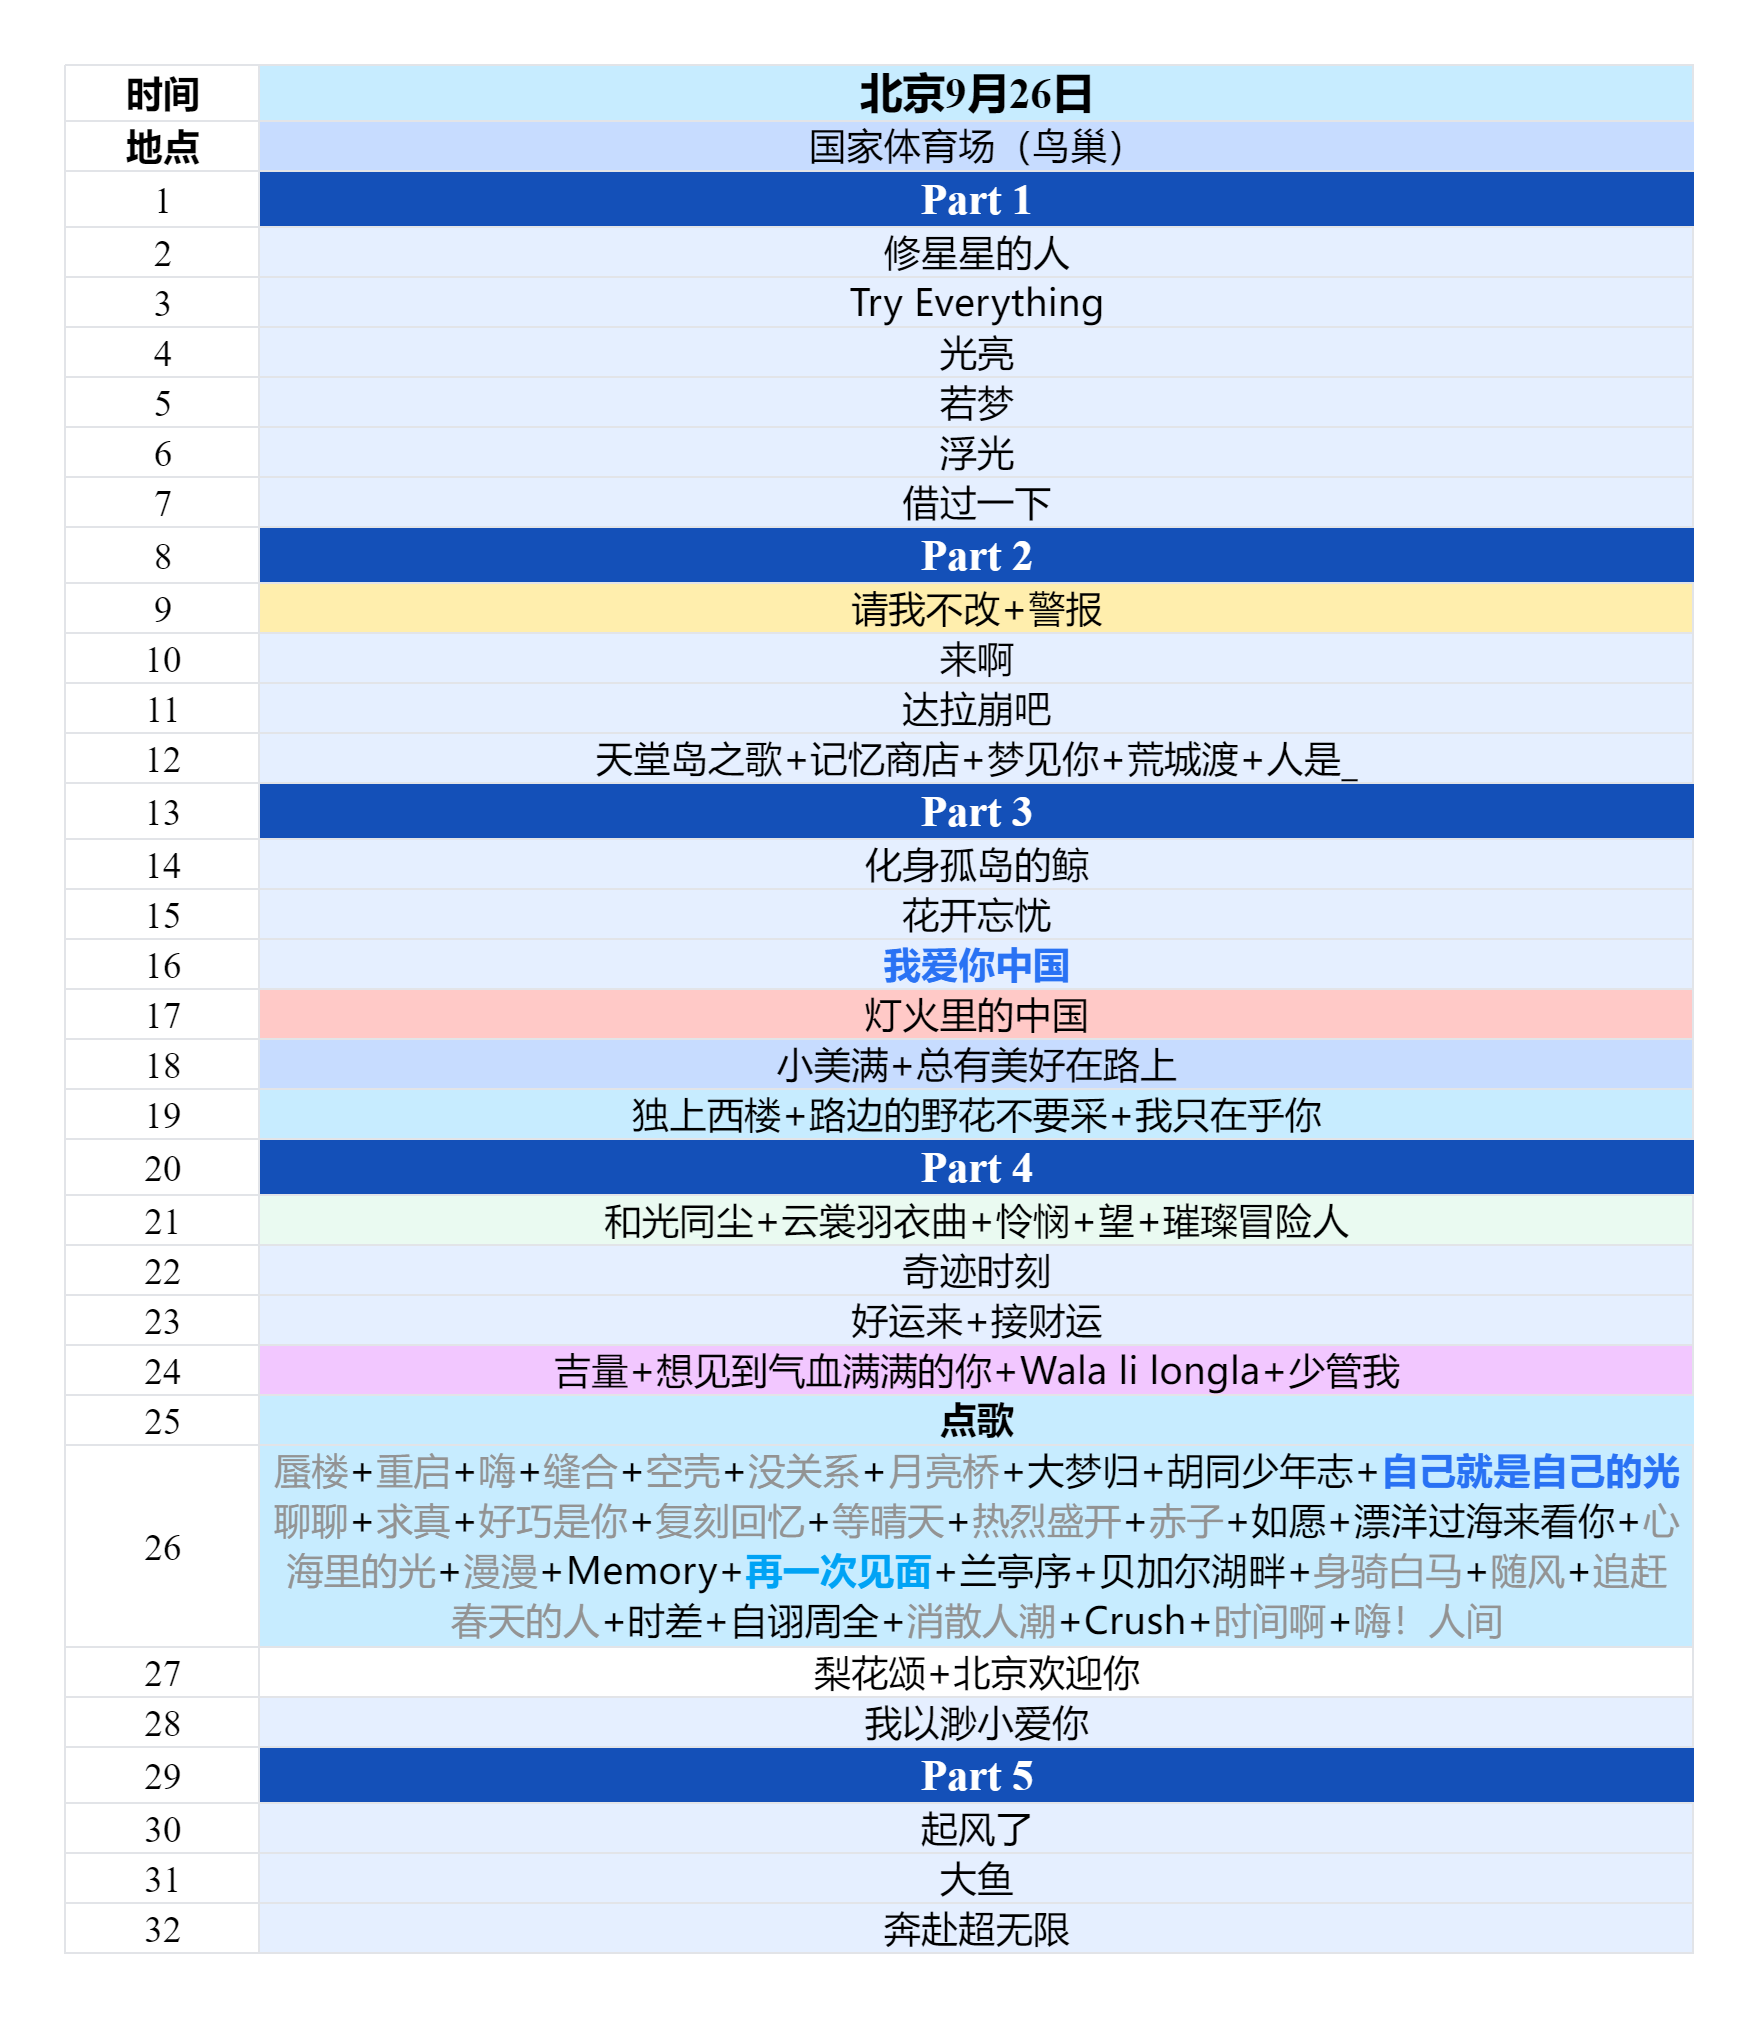
\includegraphics[width=280pt]{img/playlists/BeiJing-20260926} 

}

\caption{2026周深“深深的”巡回演唱会2026.09.26北京场歌单}\label{fig:unnamed-chunk-48}
\end{figure}

\newpage

\section{Part1}\label{BeiJing-20260926-part1}

\hyperref[opening-vcr]{🎥【\textbf{开场VCR}】}（VCR 正文见附录 D。VCR 结束后《修星星的人》前奏直接响起。）

\hyperref[xiu-xing-xing-de-ren]{🎵【\textbf{修星星的人}】}（米：先声合唱：既然这宇宙让我诞生------）（深：是我在故乡的旷野，仰望银河的夏夜；是我在宇宙的风暴，朝着天仓五飘曳；我的孤独我的热烈，源自137亿年前，几粒星尘的蝴蝶；在噬星的幻灭里，为太阳撑一把雨伞；在时间的深海里，给地球道一声晚安〔看台录音混响较大，本段唱词与附录G差异处均已照词校正，现场版个别句待核〕）北京的朋友们你们好吗！（米：好------！）（深：既然这宇宙让我诞生，想必它是要以我为证；我的情感和三十六度的体温，足以暖热即将熄灭的恒星\ldots\ldots 许我以造物的碎屑，重塑文明的边界；许我以渺小的羞怯，挽留物种的毁灭）（深：既然这宇宙予我重生，想必它是要让我看懂，我的基因和闪闪发光的记忆，足以照亮所有星际的永恒）（高音吟唱）鸟巢的朋友你们好吗？（米：好！）既然这宇宙让我们诞生，我们就勇敢的 Try Everything，好不好？（米：好！）尖叫声！（米：欢呼声）

\hyperref[try-everything]{🎵【\textbf{Try Everything}】}（深：I messed up tonight, I lost another fight\ldots\ldots No I won't leave, I wanna try everything / I wanna try even though I could fail）（深：Oh oh oh oh------）（米：Try everything）（深：Oh oh oh oh------）（米：Try everything）（深：Oh oh oh oh------）（米：Try everything）（深：Oh oh oh oh------）（深：Look how far you've come, you filled your heart with love\ldots\ldots I'll keep on making those new mistakes / I'll keep on making them every day / Those new mistakes）尖叫声！（米：欢呼声）全场！（米：Try everything!）再大声！（米：Try everything!）Try\ldots{} 鸟巢的人有多少啊？（米：欢呼声）Every try\ldots{} I try\ldots{} Every try\ldots{} Everything\ldots〔口播听写待核〕

\hyperref[silver-linings]{🎵【\textbf{光亮}】}Try\ldots{} 北京的朋友们你们好吗？（米：好------！）哇，谢谢。我们在的场馆是？（米：鸟巢！）哇，这可是鸟巢啊。是你们把一个非常非常普通的男孩带到了鸟巢开演唱会，也为自己创造的奇迹给一点欢呼声好不好？让我听到你们的声音！（米：欢呼声）没有你们这一切，我真的都做不到。后面的朋友你们好吗？（米：好------！）辛苦大家了。因为我有我有爬到过我们鸟巢后面那个位置，哇，爬到了腿酸。但是我觉得，我相信我们相遇的这一路可能比爬上那个很高的位置还要酸。所以非常非常感谢在任何时刻你们听到了我唱歌，谢谢你们！（米：谢谢周深！）来到北京，要说几句北京话。那我可就不客气了。北京豆汁儿喝了吗？（米：没喝！）没喝。到底豆汁儿是做给谁喝的呀？因为我有问我北京的朋友，我说你们爱喝豆汁儿吗？那玩意儿，爱喝不爱喝。北京烤鸭吃了吗？（米：吃了！）（观众：没有！）后面的朋友也吃了北京烤鸭吗？（米：吃了！）哦，那你们北京还有很多很多很漂亮的一些景点你们去看了吗？比如像故宫啊，有去看吗？（米：去了！）但我看过比任何景色都美丽的地方，那就是我眼前看到的你们。（米：欢呼声）谢谢你们把我的人生日记写得这么精彩。也谢谢你们在任何地方都愿意成为我的光亮。\textbf{\textcolor{red}{我爱你们}}！（米：我们也爱你！）（深：海上一阵风吹起，白云涌向陆地，季风带走沙粒；四季冷暖的交替，多鲜活的生命，有枯萎的痕迹；是奔跑中突然袭来的风雨，是黑暗中一根火柴燃烧的光明；也许你猜不透未知的宿命，像流星飞翔着它却不知目的）可是啊我却------（米：愿意相信！）最渺小最微弱最柔软最无畏的你，用尽了全力努力地回应，再无边再无尽再无解总有一线生机，光亮你自己。（戏曲念白＋唱腔两遍：莫听穿林打叶声，一蓑烟雨任平生；畅音阁里终一叙，六百年一粟，沧海一梦）谢谢你们的出现。（与观众合唱互动）后面的朋友谢谢你们。（继续合唱）最无畏的你。

\hyperref[like-a-dream]{🎵【\textbf{若梦}】}跟你们相遇美好的就像一场梦一样。你们能帮我一起大声唱若梦吗？（米：能------！）（深：浮生若梦，为欢几何；风摇雨落，此心何处停泊；剑起刀割，却斩不断这因果，看天地之间皆漠漠；尘缘萧索，宿命奈何；日升月落，此生依旧难舍；铁马金戈，也踏不碎这心火；忆前尘旧梦，任岁月消磨）到你们！（米：往事流转在你眼眸，一边遗忘一边拼凑，如我虔诚合十双手，唯愿你能得到拯救）你们唱歌太好听了！（米：欢呼声、尖叫声）（深：浮生若梦，尝尽了离合〔附录G作''长久几何''，现场唱词待核〕；一枕寒宵，饮下苦涩独酌；杯酒当歌，却绕不开这心锁；愿清欢入梦，伴此心停泊）〔合唱多轮记录〕再唱最后一次。（米：往事流转在你眼眸\ldots\ldots 唯愿你能得到拯救）你们？（米：唯愿你能得到拯救。）因为\ldots\ldots 你。你们，就是在得到拯救。（米：欢呼声、掌声）人生苦短，苦酸万甜〔口播听写待核〕。也非常开心有机会跟大家说，``宝你个头''。（米：笑声、欢呼声）因为你的出现，这世间才值得留恋哦。

\hyperref[floating-light]{🎵【\textbf{浮光}】}（深：看指尖拨响蝴蝶，扇动一场离别；我推开无声岁月，续梦一页；你我只是打个照面，可曾有过誓约，走进熟悉却陌生的思念）啊\ldots\ldots（深：你的眼眸装满了时间，你的身后拥故事成篇，此生如梦愿细数流年，与你同写沧海桑田；浮光掠影重山彩云间，你的伏线穿越千百年，人生不过恍惚三万天，漫漫人间，留恋流连）去吧\ldots\ldots 去吧\ldots\ldots 最大声！后面的朋友！〔合唱段按附录G，看台录音下应答多轮记录〕

\hyperref[excuse-me]{🎵【\textbf{借过一下}】}（深：少年扬起脸庞，前往他的月亮，人们笑他狂妄，人怎可不一样；白衣过泥潭，怎敢说不染，但凡银两有价，谁能真潇洒；少年爬上城墙，去见他的月亮，破碎几次心脏，得来几句真相；市井或朝堂，四方皆如框，若你生来有刺，磨掉再入场）你们都是对的，他说拜托，让开一下。（深、米：让我大醉一场，殿堂之上，背闲诗两三章；让我穿白衣裳，过疯人巷，去泥潭捞月光；望大人们见谅，提点的话，我懂也不想装；世人寻黄金乡，我找月亮，何必同往；话谢过，路借过，你是你，我是我）〔看台大合唱逐轮记录，``被现实凉三丈''``去你的老月光''等听写已按附录G校正〕（深：诚如先生所说，每颗心都有瑕；潇洒不是不怕，是愿付出代价；权衡利弊后，仍守对与错，谢过赐教的话，路借过一下）尖叫声！（深、米：让我大醉一场\ldots\ldots 话谢过，路借过，你是你，我是我）（高音吟唱）（深：白衣过泥潭，世故里浪漫；知心有所爱，不更改；人见过明暗，若天真犹在，当披上月光，走夜晚）你们就是我要找的月光，我找到你们啦！（米：啊------！）

\section{Part2}\label{BeiJing-20260926-part2}

\hyperref[robot-vcr]{🎥【\textbf{机器人VCR}】}（VCR 正文见附录 D。VCR 开篇日期句本场听作''2025年5月17日，今天是我被选中执行任务的第200天，系统维持正常运转的73000天''〔数字听写待核〕，其余与附录 D 一致。）

\hyperref[brave-heart]{🎵【\textbf{请我不改}】}（VCR 结束后）你们好吗？（米：好------！）尖叫声！（米：全场尖叫欢呼）〔与《警报》连唱串烧，独立条目见下〕（深：请我不改，是冒险的勇敢；请我不改，是烟火的人间；请我不改，是心跳的节拍；请我不改，是自我的独白〔现场说唱改编段，附录G无对应，听写待核〕；世界多奇怪，流言多难猜；什么是黑白，我自有安排；别想我活该，别笑我痴呆；别劝我放开，别叫我忍耐〔现场说唱段，待核〕；绝望已经大军压境，回身却没半个人影，才看清追兵与逃兵，竟都是我自己）请我不改，嘿！（米：嘿！）我的姿态，嘿！（米：嘿！）我的爱我的痛都与生俱来；请我不改，嘿！（米：嘿！）我的存在，嘿！（米：嘿！）我的明我的暗都不必躲开〔``我的命我的运哪怕无人喝彩''等现场变体待核〕；我原谅我自己，捡起遗憾拥抱无奈；我允许我放手，让我勇敢活在现在；我不等待，嘿！（米：嘿！）我不徘徊，嘿！（米：嘿！）我的笑我的泪都不再苍白，放肆盛开！Break out! Party time!（米：Hey! Hey!）High five!（深：我发送警报声，血红色惊叹号，提醒你自救\ldots\ldots 他们绝不为你而痛）〔说唱段''我把所有心酸苦涩''等与附录G差异大，待核〕（深：请我不改，我的姿态\ldots\ldots 战个痛快〔或作''坦荡痛快''，待核〕）（音乐结束，全场热烈欢呼、掌声、口哨声）哇哦！穿一下雨衣吧，不要感冒了。下雨了吗？（米：笑声、议论声）这是什么？这是我们的汗水。我们的露水，不要笑了，快穿一下雨衣。〔雨天玩笑〕欢迎大家来到深深的巡回演唱会！（米：欢呼声）

\hyperref[jing-bao]{🎵【\textbf{警报}】}〔与《请我不改》连唱串烧〕（深：我发送警报声，血红色惊叹号，提醒你自救；被遥控被耗空，快失控快断送，我替你看透；从借用到利用，到享受到滥用，转身就走，他们绝不为你而痛）〔歌中说唱段''我把所有心酸苦涩''等与附录G差异大，待核〕

\hyperref[lai-a]{🎵【\textbf{来啊}】}那接下来到了我们深深的巡回演唱会的小游戏环节。之前有一首歌，想要你们陪我一起唱。就是《来吧》〔口播作''来吧''，曲名《来啊''，待核〕，大家可以稍微学一下。在学的过程当中可以稍微穿一下雨衣，因为已经在下雨了。来啦，我唱''Don't tell me''，你们唱''来------啊''。来，Don't tell me！（米：来------啊啊啊啊啊啊！）是的是的，雨衣快来。Don't tell me！（米：来------啊啊啊啊啊啊！）也要照顾好自己哦。Don't tell me！（米：来------啊啊啊啊啊啊！）准备好了吗？（米：准备好了！）后面的朋友会唱吗？Don't tell me！（米：来------啊啊啊啊啊啊！）很重要哦，等下要靠你们了哦。那我们就一起来呀！（米：欢呼声）（深：我，我怎么就这样呆头呆脑，一不小心落入圈套，沉迷的神魂颠倒，Pass off，这灵魂乱七八糟；我，瞳孔里都是你迷人的笑，越靠越近我越浮躁，神涣散虚无缥缈，Cut stop，躁动太纷纷扰扰；天生的怪胎）（米：Yeah）（深：踌躇着徘徊）（米：Yeah）（深：太嘈杂的时代）（米：Yeah）（深：1v1较量打乱了节拍；别气急败坏，别着急淘汰，一万种防备阻碍，不如就算了，靠过来；将错就错，别拖Let's go，随你操控）Don't tell me！（米：来------啊啊啊啊啊啊！）望眼欲穿你别闪躲，再来大声！Don't tell me！（米：来------啊啊啊啊啊啊！）要爱就爱放纵吧别退缩。Don't tell me！（米：来------啊啊啊啊啊啊！）我倾尽所有赴汤蹈火。Don't tell me！（米：来------啊啊啊啊啊啊！）敢不敢直视我，Let's fall。〔两轮，One more！合唱逐轮记录〕好厉害啊！你们唱的好好。Don't tell me！（米：来------啊啊啊啊啊啊！）Don't tell me！（米：来------啊啊啊啊啊啊！）

\hyperref[dalabengba]{🎵【\textbf{达拉崩吧}】}既然这么厉害，那我们就一起来玩一下深深的巡回演唱会的小游戏好不好？（米：好！）大家可以自行选择你喜欢的颜色，用我们的荧光棒，分别是蓝色、黄色、粉色和绿色。请注意，没有红色。（米：笑声）不同的颜色代表不同的角色，分别是达拉崩吧、国王陛下、公主米娅、恶龙和倔强的人类呀。〔``倔强的人类''为红色专属玩笑，待核〕（米：笑声）不同的角色有他们相对应的台词。那等一下我喊到你们名字，你们就要喊出相应的台词好不好？（米：好！）试一下哦。达拉崩吧！（米：我最棒！）国王陛下！（米：再说一次！）公主米娅！（米：救我啊！）恶龙！（米：嗷呜嗷呜！）很棒啊。后面的朋友大声点哦。达拉崩吧！（米：我最棒！）国王陛下！（米：再说一次！）公主米娅！（米：救我啊！）恶龙！（米：嗷呜嗷呜！）这边我也看到很多红色的朋友，比如说我说北京------（米：宝贝！）（米：笑声）你们喊北京宝贝，你们不爱我了。〔玩笑〕（米：笑声、欢呼声）此题居然找到了破解的办法。〔口播听写待核〕（米：笑声）我喊北京，你们喊欢迎你，好不好？（米：好！）不好的话，那就是\ldots\ldots 是你们的宝贝吗？（米：欢呼声）解释一下啊，因为就是他们喜欢喊我宝贝，哎，已经解释不清楚了。那就北京------（米：宝贝！）你看，不用我解释了。我想让它包含着''北京欢迎你''。好来，北京------（米：宝贝！）（深：笑声）达拉崩吧------（米：我最棒！）国王陛下------（米：再说一次！）公主米娅------（米：救我啊！）恶龙------（米：嗷嗷！）〔多轮，恶龙乘以十：恶龙疼你十次------（米：嗷嗷嗷嗷嗷嗷嗷嗷嗷！）听写已校〕我们一起来回顾一下《达拉崩吧》这个童话故事吧。（深：很久很久以前，巨龙突然出现，带来灾难，带走了公主又消失不见；王国十分危险，世间谁最勇敢，一位勇者赶来大声喊：我要带上最好的剑，翻过最高的山，闯进最深的森林，把公主带回到面前；国王非常高兴，忙问他的姓名，年轻人想了想，他说：陛下我叫，达拉崩吧斑得贝迪卜多比鲁翁；再说一次，达拉崩吧斑得贝迪卜多比鲁翁；是不是，达拉崩吧斑得贝迪卜多比鲁翁；对对，达拉崩吧斑得贝迪卜多比鲁翁；英雄达拉崩吧，骑上最快的马，带着大家的希望，从城堡里出发；战胜怪兽来袭，获得十二金币，无数伤痕见证，他慢慢升级；偏远美丽村庄，打开所有宝箱，一路风霜伴随，指引前路的圣月光；闯入一座山洞，公主和可怕巨龙，英雄拔出宝剑，巨龙说：我是昆图库塔卡提考特苏瓦西拉松；再来一次，昆图库塔卡提考特苏瓦西拉松；是不是，昆图库塔卡提考特苏瓦西拉松；不对是，昆图库塔卡提考特苏瓦西拉松）〔深、米合唱穿插：于是------（米：达拉崩吧斑得贝迪卜多比鲁翁）砍向（米：昆图库塔卡提考特苏瓦西拉松）然后（米：昆图库塔卡提考特苏瓦西拉松）咬了（米：达拉崩吧斑得贝迪卜多比鲁翁）最后\ldots\ldots 救出了公主米娅莫拉苏娜丹妮谢莉红，回到了蒙达鲁克硫斯伯古比奇巴勒城；国王听说\ldots\ldots 就把公主米娅莫拉苏娜丹妮谢莉红，嫁给了达拉崩吧斑得贝迪卜多比鲁翁；啦啦，达拉崩吧公主米娅，幸福地像个童话，他们生下一个孩子，也在天天渐渐长大；为了避免以后麻烦，孩子称作王浩然，他的全名十分难念，我不想说一遍〔附录G作''要念你来念吧''，现场改词待核〕〕达拉崩吧------（米：我最棒！）国王陛下------（米：再说一次！）公主米娅------（米：救我啊！）恶龙------（米：嗷嗷！）北京------（米：宝贝！）金少刚老师------（米：Polo衫！）〔致谢预演玩笑〕安栋老师。（米：要起床！〔应答听写待核〕）和他合作。（米：我最棒！）愿意配合我说那么多离谱的话，都愿意配合我说北------京------（米：宝贝！）也是挺棒的。〔口播听写待核〕达拉崩吧的全名是？（米：达拉崩吧斑得贝迪卜多比鲁翁！）这么爱念啊。（高音吟唱）遥远彼岸天\ldots\ldots 啊\ldots\ldots〔吟唱句听写待核〕好难这一句。

在我前年〔听作''前面''，待核〕发了一张专辑叫做《反深代词》，希望大家去听一下。《反深代词》说的是两百年后的世界，有一个世界叫《反深代词》。周深呢一共有十二个不同的情绪碎片在这个世界，所以你在听这张专辑，如果你在某首歌，感觉所有的经历所有的情绪跟你一模一样的话，证明我们在《反深代词》这个世界彼此相互拥抱安慰了，所以求求大家去听一下这张专辑好吗？（米：好！）太感谢各位了。在今年呢，他的实体专辑终于跟大家见面啦！（米：欢呼声）是不是有很多朋友已经拿到啦？（米：对！）是不是有很多朋友跟我一样还在等啊？（米：笑声、附和声）如果没有听过这张，没听说过这张专辑，或者根本反什么？深什么？代什么？词？的话，求求你们听一下这张专辑。线上也可以听。那在去年，周深被困在了《反深代词》的蜃楼里面。我们来看一下，在《反深代词》这个世界又发生了什么事情好吗？（米：好！）

〔蜃楼VCR〕（叮咚，我有一个秘密，悄悄告诉你。欢迎你来到天堂入口。叮咚，有人在按门铃。是谁在外面？把恶作剧当一场游戏。听，谁在哭泣？看，谁在窃窃私语？窗外有双眼睛，他在时刻注视着你。〔低沉混响；与前两场开场口播不同，附录D未收录，建议补录〕）

\hyperref[haven-song]{🎵【\textbf{天堂岛之歌}】}（深：叮咚，我有一个秘密，悄悄告诉你。欢迎你来到天堂入口。叮咚，有人在按门铃。是谁在外面？把恶作剧当一场游戏。听，谁在哭泣？看，谁在窃窃私语？窗外有双眼睛，他在时刻注视着你。叮咚，有人在看你。叮咚，有人在看你。叮咚，有人在看你的过去。我逃不出去）生米，你在哪？（米：我们在！〔尖叫、欢呼〕）听过歌说，我在找生米，你在哪里？〔口播听写待核〕（米：在这里！〔尖叫、欢呼〕）（米：如何能分辨黑白？爱恨都要等云散。亲爱的我很抱歉。无数答案没有完美解答。〔观众合唱段，或为《记忆商店》``不朽的没有了没人记得''等句，听写待核〕）

\hyperref[the-memory-store]{🎵【\textbf{记忆商店}】}你为什么逃离你的队形？还差一点点。往左后方两步。哇！你乱得更离谱。往你的右后方两步。再来两步。再来两步。右边来一步。哇，这是\ldots\ldots 往后面走一步。哎，这是深深的巡回演唱会吗？（米：是！）哦。哦。这是《反身代词》里面的记忆商店对不对？〔听作''禁地商店''，已校〕（米：对！）他们说只要拥有这一颗米子心，就可以唤醒最喜欢的那一段回忆。跟你们相遇的每一分每一秒，都是我最爱的回忆。我曾经梦到过这样的场景，我们会对很多的暗号，比如像达拉崩吧？（米：我最棒！）北京？（米：宝贝！）哦，不是相反的是吗？哎，那这个是什么呢？〔口播听写待核〕〔唱段听写不清，唱词见附录G《记忆商店》，待人工补录〕

\hyperref[meng-jian-ni]{🎵【\textbf{梦见你}】}（深：看着眼前还年少的你，恍如流年从未淌过去；时光飞逝就算我也已老去，你却仍有着初见时那双清澈的眼睛；当再一次听你唤出我姓名，我已将一生都历尽，明白有些事情早注定；我们都站在时间的河里，离别是相遇的倒影；从初吻后的那天起，就有了再见的伏笔；我望着你远去的背影，渐行渐远直到看不清；时间会改变一切，却再也无法改变你；若多年后还能够有幸，与你重逢在另一场梦境，但愿那时你在人海里，仍将我一眼认清）〔唱词已按附录G校正〕（米：Would you love me, would you love me, sing that〔合唱拟声，听写不清〕×2轮）（观众：真会啊。〔旁人闲谈，不入正文，备注存档〕）这个是什么？很有\ldots\ldots 我也懒得接了。〔对观众席互动〕像第一次来看我演唱会的人觉得很莫名其妙。我的设定是，这是记忆商店，每个气球都代表着每个人想要唤醒的记忆。既然你这么厉害，吹两个，还可以再吹一个。鸟巢的时间很宝贵的哦。那就用一边一个膝盖，让两个气球同时做吧。〔``还在过年嘛''听写待核，或作''还在下雨嘛''〕我想想啊，那就一个膝盖和一个手肘和一个膝盖。〔口播听写待核〕来给他鼓励！（米：哇！）〔观众席吹气球互动，看台视角记录，待核〕

\hyperref[huang-cheng-du]{🎵【\textbf{荒城渡}】}（深：夜色中寻觅过，当往事困住我，也盼心中生出一点萤火；孤城的传说，有谁来过，将因果赠与我；我在等这因果，渡魂渡魄渡我；纵然已是执着难舍，断了这心魔可原谅我，宿命中获得这解脱，重来过）〔看台录音下唱词听写误差较大，已按附录G校正〕（深：眼中拂尘，手中残魂，那故事斑驳荒城；修炼天真，拨开心门，握一颗糖暖这孤身颠簸）（高音吟唱）

\hyperref[Humans_are_]{🎵【\textbf{人是\_}】}（深：未知摊开棋局，舍弃昨日才可破；再见了我的月光我的蓝我的爱；钢铁的巨兽在轰鸣，我们拒绝走入夜晚；破碎是新生的约定，我便愿为尘埃；让死亡觊觎我，让恐惧亲吻我，来摧毁我深爱的一切，可仍夺不走我的选择；弹指间湮灭我，但命运打不败活着；让生命如剧烈的烟火，璀璨熄灭前也将点亮，孩童的双眸；若巨浪已淹没了来路，我是帆亦是舟；是微渺的希望，我们依然前行，没有光指引）〔已按附录G校正〕（米：我说他们没有胆量没人记得〔合唱段，或为《记忆商店》相关，听写待核〕×2轮）（合唱/观众跟唱：让我让嘲笑笑我，我不需记得我〔与附录G''让时空消亡我，你无需记得我''对应段听写差异大，待核〕）在遇到你们之前，我也认为那些失去的才是最好的。但是听到了你们的歌声，我意识到，我们现在拥有的，我们相遇的每一分每一秒才是最值得珍惜的。你们说对吗？（米：对！）（副歌重复）（米：我说他们没有胆量把我们记得；我说他们只会用爱把我们记得〔合唱段，附录G无对应，待核〕）

\section{Part3}\label{BeiJing-20260926-part3}

\hyperref[music-animations-vcr]{🎥【\textbf{音乐动画VCR}】}（VCR 正文见附录 D，本段为纯音乐动画，无旁白歌词。VCR 前后为纯音乐过场。）

\hyperref[The-whale-who-became-an-island]{🎵【\textbf{化身孤岛的鲸}】}是因为遇到了你们，这只化身孤岛的鲸才不再孤单了。（深：我是只化身孤岛的蓝鲸，有着最巨大的身影，鱼虾在身侧穿行，也有飞鸟在背上停；我路过太多太美的奇景，如同伊甸般的仙境，而大海太平太静，多少故事无人倾听；我爱地中海的天晴，爱西伯利亚的雪景，爱万丈高空的鹰，爱肚皮下的藻荇，我在尽心尽力地多情，直到那一天）你的衣衫破旧，而歌声却温柔。（米：合唱：陪我漫无目的的四处漂流）（深：我的背脊如荒丘，而你却微笑摆首）（米：合唱：把它当成整个宇宙）（深：你与太阳挥手，也同海鸥问候）（米：合唱：陪我爱天爱地的四处风流；只是遗憾你终究，无法躺在我胸口，欣赏夜空最辽阔的不朽，把星子放入眸）（深：我是只化身孤岛的蓝鲸\ldots\ldots 我有着太冷太清的天性，对天上的她动过情；而云朵太远太轻，辗转之后各安天命；我未入过繁华之境，未听过喧嚣的声音，未见过太多生灵，未有过滚烫心情，所以也未觉大洋正中，有多么安静）哎，说不说这风是不是有点大？（米：笑声、欢呼声）你看，都把我吹成斜刘海了。〔雨天大风玩笑〕你们到底有多少个墙头？（米：没有！）很多人会好奇啊，哎，``墙头''是什么意思？就是我在问我的生米啊，你们喜欢哪些歌手啊？（米：周深！）他们会说周深。然后我说你们还喜欢其他歌手吗？（米：没有！）他们都会跟我说没有。其实有，所以我就非常不礼貌地把他们喜欢的其他歌手称为''墙头''。所以这首歌也非常好押韵，所以就问，你们到底有多少个墙头？（米：没有！）哦，无论你们有多少墙头，你们都是我的国王和王后。〔听作''国宝和\ldots\ldots{}``，按惯例校，待核〕亲爱的朋友们，我们来北京看你们哟！（米：欢呼声）我们要好好照顾好自己吗？（米：好！）要记得好好照顾好自己好不好？（米：好！）〔另有现场清唱《后来》片段''栀子花，白花瓣，落在我蓝色百褶裙上\ldots\ldots 后来，我总算学会了如何去爱''及''最炫的民族风''一句，归属与场景听写待核，疑为转场插曲，未入正文，见备注〕

\hyperref[Blossoms-that-forget-sorrow]{🎵【\textbf{花开忘忧}】}（深：巷子口买了花，穿过沿街红墙青瓦，夕阳慢慢亲吻着我的白发；推开旧木门回到家，把时光都炖香，而你只是笑不说话；一件遗憾的事就喝一碗汤；庭院深深秋叶飘落，我们苍老的时候就回到小时候\ldots\ldots 若记忆被偷走了忘了我的爱，我会说------）说什么？（米：你好吗！〔或作''你好啊''，待核〕）你们好吗？（米：好！）谢谢。〔唱词主体看台录音下听写零散，已按附录G校正〕（深：忘忧草，开着花，你在月光下不说话，一件遗憾的事就喝一杯茶，庭院深深秋叶飘落）（米：宝贝打伞！〔观众喊话，雨天〕）现场的朋友们，你们好吗？（米：好------！）在人生当中，朋友还是非常非常重要的。给自己一个拥抱，虽然大家不能相见，但是我相信，只要我们的思念够大声，他们一定听得到，你们说对吗？（米：对！）所以，希望你一定要好好照顾好自己。花开忘忧，愿你无忧。花开忘忧！（米：愿你无忧！）大家一定要注意安全，好好照顾好自己，好不好？（米：好！）大家要注意安全哦，雨衣穿好哦。

\hyperref[wo-ai-ni-zhong-guo]{🎵【\textbf{我爱你中国}】}那到北京，有太多太多太适合的歌了。哎，你们第一首会想到哪首歌？（米：北京欢迎你！）此时此刻无人在意我在说什么。〔玩笑〕那我们这首歌跟我一起唱好不好？（米：好！）因为我们现在美好的今天，我们现在拥有的一切，就是在这些风雨当中闯出来、拼搏出来的。等一下我们要唱的歌，也是我第一次站在鸟巢上唱的歌。我爱你中国。（米：啊------！）（深：百灵鸟从蓝天飞过，我爱你中国。我爱你春天蓬勃的秧苗，我爱你秋日金黄的硕果；我爱你青松气质，我爱你红梅品格）那一刻真的不敢想自己会来到鸟巢开演唱会。要唱的越大声好不好？（米：好！）（深：我爱你中国）你们？（米：合唱：我爱你中国）（深：我爱你春天蓬勃的秧苗，我爱你秋日金黄的硕果）大声唱！（米：合唱：我爱你青松气质，我爱你红梅品格）（深：我爱你家乡的甜蔗，好像乳汁滋润着我的心窝）到你们。（米：合唱：我爱你中国）再大声！（米：合唱：我爱你中国）（深：我要把最美的歌儿献给你，我的母亲，我的祖国）（深、米：我爱你中国；我爱你碧波滚滚的南海，我爱你白雪飘飘的北国；我爱你森林无边，我爱你群山巍峨，我爱你淙淙的小河，荡着清波从我的梦中流过；我要把美好的青春献给你，我的母亲，我的祖国）辛苦你们啦！（米：啊------！！）谢谢你们！（米：谢谢周深！！）〔多轮合唱逐轮记录；本曲为周深口播''第一次站在鸟巢上唱的歌''〕

\hyperref[deng-huo-li-de-zhong-guo]{🎵【\textbf{灯火里的中国}】}（米：好好听呀！）灯火里的中国，愿意跟我一起唱吗？（米：愿意！！！）辛苦你们了，谢谢你们。谢谢你们。保护好自己安全哦。（深、米：都市的街巷已灯影婆娑，社区暖暖流淌的欢乐；远山的村落火苗闪烁，渐渐明亮小康的思索；归港的船帆从灯塔掠过，追梦脚步月下交错；广场焰火在节日诉说，星空升腾时代的巍峨；灯火里的中国青春婀娜，灯火里的中国胸怀辽阔，灯火漫卷的万里山河，初心换回了百年承诺；灯火灿烂的中国梦，灯火荡漾着心中的歌）〔多轮合唱逐轮记录〕（米：哇------！！）如果风雨多，你还愿意来跟我见面吗？（米：愿意！！！）谢谢你。\textbf{一起淋过雨的人，一辈子都不会忘记的！}（米：啊------！！）（深、米：归港的船帆从灯塔掠起\ldots\ldots 灯火荡漾着心中的歌）〔合唱继续〕哇，你们还在陪我！

\hyperref[simple-bliss]{🎵【\textbf{小美满}】}啊这首，你会唱吗？（米：会！）一起大声唱好不好？（米：好！）（深、米：没什么大愿望，没有什么事要赶；看见路口红灯一直闪，它像眨眼的小太阳；乌云还挺大胆，顶在头上吹不散，我抓在手里捏成棉花糖，什么烦恼不能忘；既然是路一定有转弯，哪个风景都漂亮，揉揉疲惫的眼睛停下来看一看，美好简单）一起唱。（深、米：你看小狗在叫，树叶会笑，风声在呢喃，不如好好欣赏一秒，迷迷糊糊的浪漫；只要一觉醒来，床单洒满阳光的温暖，不去想，不必想，不用急急忙忙说一个答案）辛苦你们啦！亲爱的朋友，辛苦你啦。跟着我们继续大声歌唱好不好？（米：好！）（深、米：笑一笑就灿烂，唱一句歌就舒展，收集一点一滴小美满，都是幸福的花样；没道理的开朗，打扮平凡的日常，找到自己最合身的衣裳，只要自己够喜欢；至少还有温柔的眼光，还在夜里看月亮，心情铺得再满，也要留一扇天窗，岁月很长）最大声。（深、米：你看小狗在叫\ldots\ldots 不用急急忙忙说一个答案）我最最亲爱的你，谢谢你的出现！

（许愿环节）让我们一起在《小美满》这一首歌当中许愿吧好不好？（米：好！）像我这样，闭上眼睛，想好你的愿望。我们倒数三、二、一，睁开眼睛，你的愿望就会出现在这棵许愿树上。现场的每一个朋友，闭上眼睛，无论什么年龄段，无论什么职业，想想你想许的愿望吧。想想生日的时候，你第一个蹦出来的愿望是什么呢？闭上眼睛，想好愿望哟。要相信相信的力量，相信美好的力量，相信你们的力量。哦对了，《小美满》这首歌当中的愿望有一个要求，只能够许关于自己的愿望。想一想，是不是很久没有转过身看一下自己了？是不是很久没有感谢过自己这么的努力？是不是很久没有拥抱过自己，跟自己说一声，你真的很好，我真的应该好好的爱你。想好愿望，三、二、一，睁开眼睛。愿望都会实现的对不对？（米：对！）（深、米：你愿相信什么就把世界看成什么样，偶尔难题加点重量，也要轻轻的旋转；所以无论如何记得保管小小的光环，笑就好，哭也好，今天就是明天最好的陪伴；笑就好，哭也好，自己就是自己最好的陪伴）（深、米：你们都是周深最好的陪伴）（米：欢呼声、掌声）就算在风雨当中，我们也要祝今天生日的朋友------（米：生日快乐！）祝昨天或者前段时间生日的朋友------（米：生日快乐！）祝明天或者过段时间后面过生日的朋友------（米：生日快乐！）因为你们的出现，我才看得到\ldots\ldots{}

\hyperref[zong-you-mei-hao-zai-lu-shang]{🎵【\textbf{总有美好在路上}】}（深、米：花在开，云在飘，笑容在脸上，我们向前方一路向阳）亲爱的你，在路上慢慢逛，看太阳，让风轻轻吹拂你的脸庞。今天过去，要到明天看看结局会怎样〔附录G作''天气会怎样''，现场或为雨天改词，待核〕，雨过晴朗，故事都慢慢讲〔附录G作''阴或晴朗''，现场雨天改词〕。抬头发现，你们都是光亮〔附录G作''光一直在身上''，现场合唱改词，待核〕。（米：欢呼声、尖叫声）哎，我们现在每个人稍微搓一下手啊，辛苦大家啦，手有点冷对不对？大家一定要多多的照顾好自己好不好？身体健康是第一件事好不好？（米：好！）我们走到现在，到过很多无人知晓的角落，也一定经历了很多很多风雨。所以非常感谢每一个人，谢谢你走到了今天，我们会继续好好走下去的对不对？（米：对！）所以呢我一直有着这个目标，希望可以成为像歌手邓丽君女士一样，有好多好多歌，可以留存到你们很多回忆。如果你会唱，能不能等下跟我一起唱好不好？（米：好！）

🎵【\textbf{邓丽君组曲}】

\hyperref[du-shang-xi-lou]{🎵【\textbf{独上西楼}】}（深：无言独上西楼，月如钩。〔口播：好大的风声。〕寂寞梧桐深院锁清秋。剪不断，理还乱，是离愁，别有一番滋味在心头。）

\hyperref[donot-pick-the-roadside-flowers]{🎵【\textbf{路边的野花不要采}】}谢谢你们。你们会唱吗？（米：会！）（深、米：送你送到小村外，有句话儿要交代。虽然已经是百花开，路边的野花你不要采）全场最大声！走！（深、米：记着我的情，记着我的爱，记着有我天天在等待。我在等着你回来。千万不要把我来忘怀，千万不要把我来忘怀，千万不要把我来忘怀）你们会忘了我吗？（米：不会！）我不会忘记我们经历的每一年。因为我时常想不出来，如果没有被你听到和看到，我现在在干什么呢？

\hyperref[I-only-care-about-you]{🎵【\textbf{我只在乎你}】}（深、米：如果没有遇见你，我将会是在哪里？日子过得怎么样？人生是否要珍惜？也许认识某一人，过着平凡的日子，不知道会不会也有爱情甜如蜜？任时光匆匆流去，我只在乎你。心甘情愿感染你的气息）要笑哦！（深、米：人生几何能够得到知己？失去生命的力量也不可惜。所以我求求你，别让我离开你。除了你，我不能感到一丝丝情意）最大声！\textbf{\textcolor{red}{我爱你们}}！（深、米：任时光匆匆流去，我只在乎你。心甘情愿感染你的气息\ldots\ldots 除了你，我不能感到一丝丝情意。除了你，我不能感到一丝丝情意）你们会忘了我吗？（米：不会！）谢谢你们，我只在乎你呀！（米：欢呼声、尖叫声）

\section{Part4}\label{BeiJing-20260926-part4}

\hyperref[mask-vcr]{🎥【\textbf{面具VCR}】}（VCR 正文见附录 D。开篇日期行本场应为''2026年9月26日，北京''〔看台录音未完整收录，待核〕；VCR 结尾''你说，对吗？``与观众应答同前场。）

（米：对！）〔回应 VCR 结尾''你说，对吗？``〕没听到哦。（米：对！）你吗？〔口播听写待核〕（米：对！）

\hyperref[stay-with-light]{🎵【\textbf{和光同尘}】}（深、米：和你一起歌，和你一起合。月落星沉，日出东海。你们！）（深、米：和你走过理想的大河，从容地沸腾着）〔合唱句已按附录G校正〕（深、米：你看那盛放的花，来自期盼的种子。你看那丰硕果实，来自耕耘的浪漫。宽广的大河，来自八方汇聚的小溪。奔腾向前的大江，来自高山的哺育。和光同行，跌跌撞撞的摸索。和光同舞，奋不顾身的坎坷。和光同尘，不为盛名而来〔现场听作''不为生命而来''，已按附录G校正〕，不为低谷而去。和光同尘，为你而来。有你，我在。）

\hyperref[Song-of-the-cloud-dress]{🎵【\textbf{云裳羽衣曲}】}我们的缘分一定不会太浅，因为我的名字叫------（米：周深！）因为我的巡回演唱会的名字叫------（米：深深的！）（深、米：故事鲜艳，而缘分却太浅。我的爱恋，竟如此的明显。我不停地默念，想牢记你的容颜）大家请唱！（深、米：故事鲜艳，而缘分却太浅。这些年你又在那座红尘之间，幻化成哪张脸〔听作''哪场烟''，已按附录G校正〕）（深：你轻落指尖，月下拨弄琴弦，一曲云裳羽衣恋，人世间，漫天飞舞着思念〔听作''云起不知年月，下有忘情泉。一曲离殇，余音绵''，已按附录G校正〕）

\hyperref[lian-min]{🎵【\textbf{怜悯}】}〔尾声吟唱含''我要\ldots\ldots``等片段，唱段听写不清，唱词见附录G《怜悯》，待人工补录〕我们不要祈求怜悯，我们不要生病，要好好照顾好自己，我们都值得被好好的爱着，对不对？（米：对！）

\hyperref[Expectation]{🎵【\textbf{望}】}（深、米：我们总会绕啊绕，绕啊绕，绕几千里路也望向归途。乘着风，想念吹拂，游夜空漂浮，抓一颗流星做礼物，愿你幸福。手中线绕啊绕，绕啊绕，绕几千日夜也望向归途。燕归巢，迁徙之路，参与者无数，待到烟火照夜白时准备庆祝。我们心有所住）大声〔听作''在大山''，待核〕！（深、米：我们总会绕啊绕，绕啊绕，绕几千里路也望向归途。乘着风，思念吹拂，游夜空漂浮，抓一颗流星祝福，你要幸福\ldots\ldots 我们心有所住）〔合唱逐轮记录〕

\hyperref[adventurers]{🎵【\textbf{璀璨冒险人}】}璀璨冒险人们，你们准备好了吗？（米：准备好了！）我们一起放声高歌好不好？（米：好！）（深、米：他们说要越过前方风沙必须低着头，他们说要绕过蜿蜒的河才能往前走。他们说烫要放手，太阳要换个路口。如果得不到谁的认同那就不算拥有。没人能决定谁的一生应该怎么活，没人能定义谁的天空是什么颜色。没人未梦就先懂，只管相信就\ldots\ldots 背向光的英雄，每张轮廓，出自平凡的沉默）你们的出现，你们就是我的英雄！（米：欢呼声）（深、米：沿途一身泥泞跌撞的是我，忍痛缓行不回头的也是我。就让一路曲折每一道伤口，洗净我的脆弱。原来咽回去的泪，才能淹没了脆弱。你发誓更勇敢一生与梦相拥，还想要继续吗？要逆风不退啊〔听作''有你风不退啊''，已按附录G校正〕，让痛苦住进你眼眸。别怕未来的模样，辜负曾经的凝望。有多少理想就有多少次传唱〔听作''穿肠''，已按附录G校正〕，那沿途的风浪也不过就这样，这一路光景有你在身旁）〔合唱高音：要炙热啊，要不枉啊，要有梦啊〔``就知道啊\ldots\ldots 永不枉啊\ldots\ldots 要有梦啊''听写已按附录G校正〕〕（深、米：起风了，呼唤了，你还在等什么？挥手了，再见了，别不舍回头啊。向心中的梦啊，去追吧）（合唱高音吟唱：呜\ldots\ldots 愿你哭过，不惧脆弱〔听作''愿此去''，已按附录G校正〕）再次发自内心的感谢那么多人愿意看我的条形码刘海。〔雨天发型玩笑〕（观众笑声）希望大家不要害怕看到自己脆弱的一面好吗？（米：好！）它们也是组成最完美的我们的非常重要的一部分对不对？（米：对！）希望你勇敢、无畏、温暖、有爱，耶！（清唱：不惧脆弱\ldots\ldots）哇，好神奇。刚才我在我在唱歌的时候，就有一句歌词什么''嗯嗯，起风起风了''，然后就看见自己的嘴巴有一串水珠，起风了\ldots\ldots 我已经分不清是雨水还是我的泪水。我在想什么啊？是太感动了流出的泪水或者是雨水。但是你们一定要好好照顾好自己好不好？雨衣穿好。因为被你们听见的我，哦，每一分每一秒都是奇迹时刻。（米：欢呼声）

\hyperref[miracle-moment]{🎵【\textbf{奇迹时刻}】}（深：从银河抹去的恒星，穿梭时空的王牌，一个瞬息就能将不思议解开〔现场听写与附录G差异大，已照词校正；看台录音下本曲唱词多为现场变体，待核〕\ldots\ldots 这世界总有太多陆离光怪，以惊喜回应期待，We can dream, we can fly；若相信谁都可以重塑现在，不需要等待，Show time，此刻就无限精彩；I wanna see my way in starlight，奇迹时刻等你一起来；We gonna change the fate never deny，以无数颗渺小的光彩，就能照亮无穷未来）〔两轮，含现场增唱段''这一刻这一秒这一瞬间，只有我们自己才懂得\ldots\ldots``等，附录G无对应，待核〕我要开始变魔术了你们准备好了吗？（米：准备好了！）我这个魔术一定会成功。鼓励我的掌声在哪里？（米：欢呼掌声）【魔术环节】这是一个非常普通的丝巾对不对？很真实的丝巾对不对？（米：对！）这是一个没有任何问题的圆柱体对不对？它是没有毛病的对不对？没有问题吧？这边穿不过去对不对？（米：对！）那你们看这条牌，特写。我现在把这个丝巾把它塞进这个孔里，没有问题吧？把它穿过去哦，没看到没问题对不对？来看咯。给我倒数三个数字。三！（米：二！一！）啊！耶！三、二、一！没有啦！还有，过来看。提前穿帮了！〔魔术失败自嘲〕（歌曲《好运来》前奏起）

\hyperref[good-fortune-comes]{🎵【\textbf{好运来}】}（深：叠个千纸鹤，再系个红飘带，愿善良的人们天天好运来。你勤劳生活美，你健康春常在，你一生的忙碌为了笑逐颜开\ldots\ldots）（高音吟唱）（米：欢呼声、掌声）暂时用我的高音掩盖一下自己收到这个\ldots\ldots 怎么回事？到底怎么回事？而且，我就是前面两次变失败那个魔术还在这里。我们尝试一下变这个好不好？一个魔术总不能失败三次吧，来特写。大家看哦，哎哟，差点直接\ldots\ldots 哎鼓手不要击鼓了仿佛在阴阳怪气我。〔玩笑〕啊，现在四个骰子，四个骰子没有任何问题对不对？没有问题啊。你看，现在是看不出来问题的，看不出来问题是吧？掌声在哪里？（米：掌声、欢呼声）看咯，三、二\ldots\ldots 好紧张。是这里吗？（米：哇------！）可是我要变的是这边多出一个呀。刚刚已经看过是不是？那个时候我就错了是不是？大家看，大家看，现在是不是还剩三个了？大家看哦，等我三个数字，三、二、一。（米：笑声）等一下，别说话，我在弄心法。〔玩笑〕那三、二、一。（米：笑声）谢谢大家！好运来了，大家接不接？（米：接！）（深、米：好运来祝你好运来，好运带来了喜和爱，好运来我们好运来，迎着好运兴旺发达通四海）（深：叠个千纸鹤，再系个红飘带，愿善良的人们天天好运来。你勤劳生活美，你健康春常在，你一生的忙碌为了笑逐颜开。打个中国结，请春风剪个彩，愿祖国的日月年年好运来。你凤舞太平年，你龙腾新时代，你幸福的家园迎来百花盛开）身体健康，接不接？（米：接！）恭喜发财，接不接？（米：接！）（深、米：叠个千纸鹤\ldots\ldots 迎来百花盛开）现场的朋友们！好运来了接不接？（米：接！！！）大家一起用最大的声音，接所有的美好，好不好？（米：好！！！）准备好了吗？（米：准备好了！！！）一起，接平安！（米：接平安！）接幸福！（米：接幸福！）接健康！（米：接健康！）接财运！（米：接财运！）

\hyperref[jie-cai-yun]{🎵【\textbf{接财运}】}（深、米：接个好运来，接个福气来，接个财神开开心心到家里来。接个财运来，小财大财，我接我接，我接金山银海）〔合唱：好运来，我接个好运来\ldots\ldots 我接个满堂彩〔后段听写待核〕〕祝鸟巢的朋友，恭喜发财！接不接？（米：接！！！）哦，谢谢你们！（米：欢呼声）哦，因为天气的原因，我没有办法去看到我们后面的朋友，你们好吗？（米：好！！！）所以我想要听到你们的声音，后面的朋友你们好吗？（米：好！！！）所以可能很多很多事情，真的没有办法所谓的完美，或者是怎么样，但是有的时候顺顺利利的过去就非常非常幸福。然后我也觉得自己是个非常幸福的人，因为有那么多人愿意陪我一起去面对。谢谢每一个最可爱的观众朋友！（米：欢呼声）也希望你们要知道哟，身体健康，平平安安，照顾好自己永远是最最最最最重要的事情，好不好？（米：好！！！）那等一下，用最大的声音跟我接，马年无量的吉祥，好不好？（米：好！！！）

\hyperref[ji-liang]{🎵【\textbf{吉量}】}（深、米：羲和车上金铃铛〔看台录音听作''河水洋洋，万顷凉''等，已按附录G校正〕，叮当叮当；望舒驾后银尾巴，摇摇晃晃；弱水岸边唤吉量，吉量吉量，叮叮当当，天地叮叮当当）（深：九天之上飘来一朵雪花，原来是我那英俊的小马；金色星星在它眼里安家，祝融手持火种编织了它的发；我的小马一天一天长大，穿过凛冬和最沸腾的夏；衔来西边石头东边的花，马蹄扬起层层层层的云沙）你们好！（深、米：吉量，我勇敢的小马〔合唱段听写误差大，已按附录G校正；完整逐轮记录待人工补核〕\ldots\ldots 吉量，树顶上那颗太阳，在晨雾里张望，驮它来我身旁）〔看台录音下本曲合唱段听写误差较大，正文已按附录G骨架整理，建议人工补核〕

\hyperref[xiang-jian-dao-qi-xue-man-man-de-ni]{🎵【\textbf{想见到气血满满的你}】}〔唱段与《吉量》在转写稿中交叠，已按附录G校正〕（深：有时候感觉自己多珍贵，还会有更好的等着你，还有好多梦在飞，还要给自己一个新的机会。要早起早睡，别那么累，做好气血满满的准备；想见到你，灿烂的你，无惧也无畏；别害怕疼痛，别怕眼泪，就让我来陪着你找回，手里有暖，心里有暖，阳光的明媚）全场朋友！〔与观众''你是谁？你是自己的------宝贝！``互动，看台录音记录不全，待核〕

\hyperref[wala-li-longla]{🎵【\textbf{Wala li longla}】}全场的宝贝你们好吗？（米：好------！）后面的宝贝们你们好吗？（米：好------！）三楼的宝贝们你们好吗？（米：好------！）我也是突破自我了，真的。鼓起勇气喊你们，宝贝！（米：啊------！）你是谁？你们是周深的------（米：宝贝！）我有这么多宝贝，我是怎么好意思说人家有很多墙头的。〔玩笑〕在我的专辑有个快乐密码，你们跟我一起念哦。Wala li longla!（米：Wala li longla!）后面的宝贝们。Wala li longla!（米：Wala li longla!）全场最大声，Wala li longla!（米：Wala li longla!）（深：把蜗牛都放大，把汽泡堆成塔，口味自由混搭，用沙砾提炼火花；无所谓章法，无所谓多伟大，一默念就触发，Wala li longla）〔现场版唱词与附录G差异大：``把梦境都放大，把寂寞对折''``终点注定是谜团成麻，稀里哗啦''``全世界追着给节奏加码''``让云擦肩飞过希腊''``哪怕我只是浪花，也包裹进时空的无价''等，待核〕你们好吗？（米：好------！）我来啦！Hello!全场的宝贝你们好吗？（米：好------！）周深，我真的受不了你啦！〔口播自嘲〕跟我一起大喊这个快乐密码好不好？（米：好------！）全场，Wala!（米：Wala!）Wala li!（米：Wala li!）Wala li long!（米：Wala li long!）Wala li longla!（米：Wala li longla!）〔逐词递进教学多轮；对喊交替：深：Wala li longla! 米：Wala li longla! ×10余轮，含''宝贝！``\,``上面的朋友！''``全场！''口令〕（合唱：Wala li longla，快乐在脚下，心里有花啦〔现场版唱词，待核〕；全世界随你节奏变化，管他开心吧还是悲伤吧，反正都一样〔现场版唱词，待核〕；心里有花啦）你们好吗？全场的宝贝，最后一遍，Wala li longla！（米：Wala li longla!）

\hyperref[watch-ur-manners]{🎵【\textbf{少管我}】}我们还有一个暗号哦。三、二、一，嘿！（米：少管我！）少管我！嘿！（米：少管我！）全场最大声，三、二、一，嘿！（米：少管我！）（合唱：嘿，少管我。嘿，少管我。嘿，少管我）〔现场版听作''别来烦我''，已按附录G校正〕（合唱：有什么关系，删掉无聊的理由〔听作''你说的那些无聊的理由''，已按附录G校正〕；把沉重身体传送到热带气候〔听作''画成圆点圈住那个借口''，已按附录G校正〕，脑袋放空，吹吹海风；用一场远行当做逃离的方舟〔听作''摆脱透明的困兽''，已按附录G校正〕；做生活困兽不如去浪漫宇宙，烦恼忧愁，全部都清空）宝贝们你们好吗？（米：好！）（合唱：看霓虹长出柔软的触角，给单调的人换上缤纷躯壳〔听作''哪怕此刻感到无助，也要让生命更倔强''，已按附录G校正〕；下一步向左向右，看心情都不重要；下个绿灯亮起做信号，越过人山人海直奔那街道〔听写与附录G差异大，待核〕）我们一起！（合唱：我想我可以抓住风中飘散的花，不介意坠入水星或是泥巴；跟现在握手拥抱，道别出发，别停下）再来！（合唱：我想我成为阳光、蔷薇、飞鸟、盛夏，或成为昆虫、沙砾、一片雪花，我不在乎，将烦恼都忘掉）宝贝们，三、二、一，嘿！（米：少管我！）三、二、一，嘿！（米：少管我！）后面的宝贝们，三、二、一，嘿！（米：少管我！）全场，三、二、一，嘿！（米：少管我！）最大声，三、二、一，嘿！（米：少管我！）（合唱：找最真的自己\ldots\ldots〔结尾段听写与附录G''将这段旅途，献给那些不堪重负做礼物''差异大，待核〕）（高音吟唱）三、二、一，嘿！（米：少管我！）让我用我的气泡音。（气泡音）不愧是我的老粉。〔自嘲〕谁来管管这个周深啊。〔口播〕真的好\ldots\ldots 呃\ldots\ldots 行。掌声给我们的舞者们！

【\textbf{点歌环节}】接下来到了我们的点歌环节。我们一起倒数五个数字好不好？好，全场，五！（米：五！）四！（米：四！）三！（米：三！）二！（米：二！）一！（米：一！）耶！哦？（米：哇------！）哦，在哪里呀？哇！你好。（婷婷：你好，周深老师。）您的头发是平时就这样梳的，还是因为打湿了这样梳的？（婷婷：打湿的。）也变成条条吗？谢谢你啊。你这条条扫过去有我这个精准吗？〔``条形码刘海''梗，口播听写待核〕请问怎么称呼您？（婷婷：嗯，叫我婷婷就好。）婷婷。（婷婷：对，婷。）哦，往这边站一下，让我看清楚一点。来自哪里的朋友？（婷婷：呃，来自山东济南。）（米：欢呼声）验证一下。（深哼唱：鲁A济南车\ldots\ldots）鲁B青岛的。她这个''青岛''很标准。哦，应该经常来到北京吧？离得很近。（婷婷：嗯，对，是的。）那有去看我在济南的时候的演唱会吗？（婷婷：嗯，有的有的。）哇，真的有啊？（米：合唱：天下相亲与相爱\ldots\ldots〔观众以济南场曲目《相亲相爱》应答〕）刚才是替我在唱是吧？谢谢你。哎，你是婷婷对吧？那你第一次听到我的歌是哪首歌？（婷婷：呃，《大鱼》。）哦！现在有记，就是已经有非常有标准的两个问题，记词儿还是不记词儿？（婷婷：呃，记词儿吧。）记词儿。记词儿，那我们\ldots\ldots 记词儿八，对不对？为什么记词儿八呢？比如说不记词的那段。（示范高音吟唱：啊\textasciitilde\textasciitilde\textasciitilde\textasciitilde\textasciitilde\textasciitilde\textasciitilde）婷婷你唱。（婷婷尝试高音：啊\textasciitilde\textasciitilde\textasciitilde\textasciitilde\textasciitilde\textasciitilde\textasciitilde）（米：观众欢呼喝彩）你是来踢馆的吗？你刚听那个麦克的时候，我听见了非常清楚的两个字，``哎呀''。那就不要往心里去了。〔口播听写待核〕（示范高音：啊\textasciitilde\textasciitilde\textasciitilde\textasciitilde\textasciitilde\textasciitilde\textasciitilde）（婷婷：这个我真的唱不上去。）真的唱不上去，清嗓都白清了。〔玩笑〕（示范更高音：啊\textasciitilde\textasciitilde\textasciitilde\textasciitilde\textasciitilde\textasciitilde\textasciitilde）那就是你要来吃好吃的。多吃点好吃的好不好？今天是一个人来的吗？（婷婷：一个人。）谢谢你。那第几次来到北京？应该经常来吧？是吗？（婷婷：很多次了。）哦，哇！很多次都是看别人演唱会吗？（婷婷：没有。）第几次来到鸟巢啊？（婷婷：第一次来到鸟巢。）第一次来鸟巢看演唱会吗？（婷婷：对。）哇！谢谢她！这里有多少是第一次来到鸟巢看我们演唱会的？（米：全场热烈欢呼）哎，有首歌说得好啊。（深、米：合唱：第几次来没关系，有太多话题\ldots\ldots〔《北京欢迎你》现挂〕）不管是第几次来看演唱会，都谢谢你来跟我们见面，谢谢大家！那婷婷帮我们点出今天的第一首歌好不好？（婷婷：嗯\ldots\ldots《自己就是自己的光》。）（米：全场欢呼）谢谢。也希望大家一定要照顾好自己好不好？一定要记住你们一直在发光发亮好不好？（米：好！）你们好不好？好不好宝贝们？（米：好！）终于还是迈出了这一步。〔口播待核〕谢谢婷婷，那在深深的这片海洋里〔口播待核〕留下你灿烂的笑脸好不好？（婷婷：还有最后一句话。）哎，你好。（婷婷：祝周深宝贝生日快乐！）（米：全场欢呼祝福）谢谢。然后我的妆被顶到这里都快像没有了，你们也不愿意听我唱歌吗？〔雨天妆容玩笑〕（米：愿意！）那我问的什么问题啊？你们是来听唱歌的还是来看我的妆容的是吗？来，留下你的灿烂笑脸哦。三\ldots\ldots 呃，可可的脸，你要决定把它露出来吗？〔``可可''梗〕好，三、二、一，耶！（婷婷：呜呼！）这张可以吗？谢谢婷婷，谢谢你。也谢谢跟婷婷一样的这么多的好朋友跟我们见面，这一切的一切都是因为你们才能够发生。谢谢你们！一定要记住，你们是自己的光，好不好？（米：好！）好不好宝贝？（米：好！）

\hyperref[zi-ji-jiu-shi-zi-ji-de-guang]{🎵【\textbf{自己就是自己的光}】}（深：嘿，去有山的地方，别让心四处流浪；嘿，看海角的风光〔听作''看海角的疯狂''，已按附录G校正〕，别放弃向远眺望〔听作''别放弃少年骄傲''，已按附录G校正〕；我们都曾经历过至深至暗的荒凉，嘲笑如蜃楼迷墙〔听作''迷障''，已按附录G校正〕，连同狂风和骤雨，也不能阻止飞翔）〔唱段主体看台录音下听写不完整，已按附录G校正，待人工补录〕

（第二位点歌）我也没穿这身，不好意思，你好。请问怎么称呼您？（新桥：呃，叫我新桥吧。）新桥？（新桥：嗯。）新桥你好，是来自哪里的朋友？（新桥：天津。）天津啊，哎呦，这么远。带课吧？〔听作''带课''或为''带快板了吗''，待核〕（新桥：没有。）没有，那带了一段贯口吗？（新桥：啊。）啊啊，不知道。哦，跟你们聊天特别厉害你知道吗？〔口播听写待核〕那那你用最地道的天津话给大家打个招呼，欢迎大家来到深深的巡演演唱会好不好？（新桥：欢迎大家来天来北京。）本来是想让你欢迎大家来北京的，骗你的，开玩笑的。好啦，今天是一个人来的吗？（新桥：呃，还有我妈妈和我好朋友。）她们在哪里？（新桥：呃，我妈妈在我旁边，然后我好朋友在看台上。）好朋友，加油。（米：加油！）你们好漂亮哦。（童颜：你好。）怎么称呼您？（童颜：主持人好。你好。我我叫童颜。）童颜？哇，人如其名啊，哇。好的，谢谢您的支持。今天是我们新桥的点歌机会，你第一次听的歌是哪首歌呀？（新桥：大鱼。）应该很熟悉吧？（新桥：都可以。）那咱就看你来唱。（新桥清唱《大鱼》片段：海浪无声将夜幕深深淹没，漫过天空尽头的角落\ldots\ldots）什么意思？什么意思？（米：抢了饭碗。〔观众玩笑〕）我刚才有听到为你的欢呼声，听到了吗？（新桥：谢谢大家。）你唱的真的很好听，大家再给新桥一点鼓励！真棒，那我们点今天的第二首歌好不好？（新桥：呃，可以跟你说两句话吗？）可以可以可以。（新桥：呃，就是首先祝你生日快乐。）我想用我想要天津口音听后面所有的话。说吧，人家天津话不这么说的。你说吧，可以用天津话吗？（新桥：不要。）好来吧。（新桥：呃，首先祝你生日快乐。然后祝你能唱到反身代词世界的那个时候。）你祝我唱两百年啊？那我要是唱两百年，我也要求求你们一起跟我听我唱两百年好不好？（米：好！）新桥你好会说话哦，谢谢。（新桥：然后我是艺考生，我是因为你选择这条路，然后希望你能不能祝我艺考顺利。）哇什么时候考？（新桥：嗯明年十二月。）你就把这一段寄给老师。大家说我们新桥唱得好不好？（米：好！）当然还是要看你到时候考得好不好，然后但是我们的观众朋友们都会为你加油打气的对不对？（米：对！）我们一起祝我们新桥艺考------（米：顺利！）好不好？加油！好好展现自己哦，所有一切都是最好最好最好的安排。帮我们点出今天的第二首歌吧。（新桥：呃我想听再一次见面。）（米：哇------！）谢谢你。（米：我们会如约再一次见面的！〔观众齐喊〕）（米：哇------！）现在的艺考生都这么会说话，我又说不过了，唱也唱不过真的是。那让我们留下你灿烂的笑脸好不好？对，哦好棒啊，还有爸爸妈妈。问我们的童颜女士要不要一起合照？看我们前面的摄像老师哟。童颜女士我们看前面啊，那个摄像摄像机。对对对对就在你面前。来咯，三二一，耶！这张可以吗？可以啊，好谢谢你！谢谢新桥，谢谢你，谢谢童颜女士。我也不知道刚才那一段片段能不能拿去艺考有用啊，大概率应该是没什么帮助。但是你要知道哟，那么多人都说你唱歌很好听，要继续好好的去找到自己好不好？哇全程埋头不敢看你说这种话。〔口播待核〕大家再给我们新桥鼓励让她加油，三二一新桥！（米：加油！）最重要的是也要为每一个你们自己加油，和每一个最可爱的自己！（米：加油！）

\hyperref[zai-yi-ci-jian-mian]{🎵【\textbf{再一次见面}】}（深：喜欢你已经很久很久，久到习惯在你身后；爱消失了以后〔听作''爱像是个迷宫''，已按附录G校正〕，我都没想过回头；或许分开有很多理由，只是却不曾在乎我的感受，那句挽留我始终开不了口；再一次再见，再说一句再见，在我没反悔之前〔听作''没防备之前''，已按附录G校正〕；再一次失眠，再无法停止对你的思念；再一次划清作为普通朋友界限，当你退出那天；再一次见面，再说好久不见，再坐下来聊聊天；在你的身边，再一次习惯回避你视线〔听作''把你的身影再一次希望回忆里实现''，已按附录G校正〕；再最后我不得不对你说一句谎言，我会忘了你，一直到永远）你们会忘了我吗？（米：不会！）（深：再一次再见\ldots\ldots 我会忘了你，一直到永远）你们会忘了我吗？（米：不会！）真的谁来管一下这个场面。〔口播〕一直到永远。

\hyperref[li-hua-song]{🎵【\textbf{梨花颂}】}那要说到点歌，有一首歌来到鸟巢的时候，大家在网上点了无数遍。等一下如果你们会唱跟我一起唱好不好？（米：好！）（深：梨花开，春带雨；梨花落，春入泥；此生只为一人去；道他君王\ldots\ldots）

\hyperref[bei-jing-huan-ying-ni]{🎵【\textbf{北京欢迎你}】}你们愿意跟我一起大声唱出《北京欢迎你》吗？（米：愿意！！！）一！（米：二！三！）大家跟我一起大声唱好不好？（深：迎接另一个晨曦，带来全新空气；气息改变情味不变，茶香飘满情谊；我家大门常打开，开放怀抱等你）你们！（米：拥抱过就有了默契，你会爱上这里）再大声！（米：不管远近都是客人，请不用客气）大声！（米：相约好了在一起，我们欢迎你）（深：我家种着万年青，开放每段传奇；为传统的土壤播种，为你留下回忆；陌生熟悉都是客人，请不用拘礼；第几次来没关系，有太多话题）准备咯！（米：北京欢迎你，为你开天辟地；流动中的美丽充满着朝气）再大声！（米：北京欢迎你，在太阳下分享呼吸）好，挥动那里！〔口播待核〕（米：在黄土地刷新成绩）谢谢大家把我的生日季写得这么精彩，也一定要写好自己的人生日记好不好？（米：好！！！）谢谢你们为我创造的奇迹，也一定要继续为自己创造更多奇迹好不好？（米：好！！！）在这片刷新无数奇迹的黄土地，喊出加油！三、二、一！（米：加油！！！）（深：我家大门常打开，开怀容纳天地；岁月绽放青春笑脸，迎接这个日期；天大地大都是朋友，请不用客气；画意诗情带笑意，只为等待你）（米：北京欢迎你，像音乐感动你，让我们都加油去超越自己）我听不到！（米：北京欢迎你，有梦想谁都了不起，有勇气就会有奇迹）全场！（米：北京欢迎你，为你开天辟地\ldots\ldots）再来！（米：北京欢迎你，像音乐感动你\ldots\ldots 有勇气就会有奇迹）那口气破得有点太长了。〔口播玩笑〕谢谢我们亲爱的\ldots\ldots 宝贝。真是受不了，豁出去了就是这个样子的，真的，开心就好，你们玩得开心吗？（米：开心！）

（周可可/周嫑嫑环节）掌声欢迎我们的周可可和周嫑嫑。然后这个周可可，他是一位非常厉害的巧克力大师，厉害到完全不正眼看我一眼。〔玩笑〕明白吗？但是他叫周可可不是因为他巧克力做得很厉害，而是因为他不会拒绝别人。任何人找他帮忙，任何人哦，就路过的一个陌生人，哎，周可可帮个忙，他会说，可以啊，可以啊，可以啊，可以啊，可以啊。他想让所有人都开心，去满足所有人的情绪，就是想让他们大家都开心。那怎么可能呢对不对？哪怕他用尽全力啊，倾尽全力，别人还是会不开心，甚至可能都没有看到他的付出。所以在他非常非常难受，已经将自己撕裂的那个过程当中呢，帮他做出第一锅巧克力的平底锅，周嫑嫑就出现了。这有多得瑟了现在已经。〔玩笑〕周嫑嫑的''嫑''字怎么写呢？上面一个不，下面一个要。所以在周可可非常难受，整个崩溃的状态，周嫑嫑帮他说出了人生当中的第一个------（米：不要！）所以想告诉你们，我们心中都有那个非常善良、可爱，然后天真，非常非常无畏的周可可，但是我们也一定要让我们心中的周嫑嫑保护好她，好不好？（米：好！）一定要做有牙齿的温柔好不好？（米：好！）也辛苦我们所有的观众朋友，包括今天我们可以开心欢聚在这里的所有的人们。

（致谢）首先感谢，想让大家一直提醒大家，一定要记住你们是自己最珍贵的宝贝的我们今天晚上的独家冠名的云南白药！（米：哇！）（深唱：云南白药提醒您，要早起早睡，别那么累，做好气血满满的准备。）好不好？（米：好！）感谢北京市所有职能部门的大力支持。（米：哇！）感谢我们的场地方，国家体育场，鸟巢！（米：哇！）心想，你也在鸟巢唱过歌哟。〔口播听写待核〕感谢本次巡演的出品方周深工作室。（米：哇！）谢谢大家。也感谢本次巡演的出品方时代立方！（米：倒闭！〔反讽应答，同常州场''倒闭''梗〕）感谢演唱会制作单位必应！（米：必应！）感谢总导演周佑洋。（米：哇！）感谢我们的总导演庄惟惞。（米：哇！）接下来要感谢这个人呢是当年零八年奥运会的时候的音响师，也是我们演唱会的音响总设计，然后我们的音响总监。你们知道吗？鸟巢近几年开了非常非常多的演唱会对不对？（米：对！）他才是来鸟巢来最多场的那位艺人。〔玩笑〕因为鸟巢\ldots\ldots 它能够把我们的声音传递很清楚，但是如果没有非常优秀的音响总监的话，传递过去的声音可能也没有那么好听对不对？所以让我们掌声感谢我们的音响总监金少刚老师！（米：哇！）时常在想啊，叫，这个地方叫鸟巢，它一定住了一只非常厉害的百灵鸟，哦，原来是金少刚老师啊，哦，金少刚老师。（米：Polo衫！）金少刚老师。（米：Polo衫！）金少刚老师。（米：Polo衫！）谢谢啦。那接下来感谢的是我们的音乐总监，也是上海音乐学院的教授，也非常非常厉害的是当年零八年奥运会这个点亮火炬的时候的那个音乐是他创作的哟。（米：哇！）感谢我们的音乐总监安栋老师。（米：哇！）安栋老师你怎么在小西装外面穿一件雨衣呀？安栋老师你答应我们的军大衣什么时候？哦，是说明天是吗？（米：〔听写待核〕）六，六十六，什么意思？啦啦，哦，是说啦啦啦啦啦啦，我听不清楚你在说什么啦。〔口播听写待核〕好的，感谢我们的音乐总监安栋老师。（米：哇！）安栋老师。（米：小西装！）安栋老师。（米：小西装！）安栋老师。（米：小西装！）谢谢你愿意陪我玩这些内部梗啊，谢谢。也掌声感谢我们的乐队老师们！（米：欢呼声）他们跟我一样非常的热爱我们每一位观众朋友。感谢我们的和声老师们！（米：欢呼声）谢谢，感谢我们的舞蹈团队SDT Show Pro！（米：欢呼声）感谢我们的服装团队劳伦斯许工作室、Third Studio、Windowsen！（米：欢呼声）感谢音响工程南京奥斯泰！（米：欢呼声）感谢\ldots\ldots 你们在蓄力。（米：笑声）你们这些人。〔预判''倒闭''应答的玩笑〕感谢我们的调音团队乐尔工作室！〔听作''乐耳''，已校〕（米：欢呼声）还在蓄力。感谢我们的硬体工程北京立超舞台集团！（米：欢呼声）感谢票务总代理大麦！（米：倒闭！）感谢票务代理猫眼、票星球！（米：倒闭！）感谢社交媒体微博、微博音乐、微博演出！（米：倒闭！）求你们了。〔口播〕也感谢他们提供的情绪价值，然后让我们可以开开心心见面。然后演出结束后大家也可以就是到微博我的微博超话当中去实况热聊里一起分享一下你的人生日记好不好？（米：好！）北京的雨冷不冷？（米：不冷！）辛苦大家了，谢谢你们。感谢所有现场台前幕后的工作人员们！（米：欢呼声）以及感谢我们现场服务我们帮我们去引导然后让我们好好见面的所有的工作人员们！（米：欢呼声）感谢北京！（米：巨大欢呼声）最重要的是要感谢每一个让这一奇迹全部发生，灯光亮起，舞台搭起来的每一个到达我们北京现场的每一个最可爱、最善良、最温暖、最帅气、最美丽、最无畏、最完美、最最勇往直前、我最爱的也是最有力量的最有爱的每一个到达现场的------你你你你你你你你你你你你你你你你你你你你你你你们！（米：尖叫欢呼声）

（大合照）嘿，宝贝。（米：尖叫声）感受到了我的愧疚感了是吧？那我们一起来大合照好不好？（米：好！）谢谢你们。哦对了，我们先看这里啊。哇，好厉害。来我喊我们在，你们说深深的，好不好？怎么没有人笑？〔口播待核〕我们在------（米：深深的！）Hello！（米：欢呼声）大家不要生病了哟。我们在------（米：深深的！）Hello！宝你个头！我们在------（米：深深的！）谢谢你们，谢谢你们一直陪着我。我在------〔口播待核〕（米：热烈的盛开！开在荒野开在小小角落与人海！）〔与观众对唱《热烈盛开》〕闪耀起未来------（米：我有我姿态！）〔《热烈盛开》合唱，``闪耀起未来''句听写待核〕好了，拍照了拍照了啊。我们在------（米：深深的！）嗨！（米：欢呼声）你们好！我们在------（米：深深的！）（米：欢呼声）你们好！我们在------（米：深深的！）鸟巢的朋友，我们来咯！（米：欢呼声）我会热烈的------（米：热烈的盛开！开在荒野开在小小角落与人海！）闪耀起未来------（米：我有我姿态！）（米：想要海上会有光为我而来！〔听写待核〕）我来啦！（米：欢呼声）谢谢你们，谢谢你们在。我们在------（米：深深的！）Hello！（米：欢呼声）谢谢你们。我们在------（米：深深的！）Hello！（米：欢呼声）我们在------（米：深深的！）谢谢每一个最可爱的你！

\section{Part5}\label{BeiJing-20260926-part5}

\hyperref[loving-you-in-my-humble-way]{🎵【\textbf{我以渺小爱你}】}谢谢你们，看到了渺小的我。也许你也会觉得自己渺小，不要害怕。我们这么多人聚在一起，我们已经做了非常非常多非常伟大的事情。比如，你们把一个非常普通、非常普通的男孩，送到那么多舞台去唱歌，让大家听到。我站上的每个舞台，都是你创造的奇迹。所以一定要知道，你的出现，就已经有了最大最大的意义好吗？（米：好------！）谢谢你们给我作为歌手这一段旅程。也谢谢你们愿意谅解我的力量有的时候没那么强大。也谢谢你们愿意谅解我们的不完美。但是请相信，我们一直在用心，感谢着你们，爱着你们。谢谢你们！（米：欢呼声）也谢谢你，愿意让我以渺小爱你。（米：欢呼声）（深：我以渺小爱你，同行的旅程）（深：最美丽的风景，从不会关上门，天空荒原大海和人生；路上做个孩子，又明亮又单纯，如小鹿一样看星辰；海风送给岛屿，几亿万年的吻，大雨落山川，像心跳声；世界那么大，我是短短的一瞬，以渺小爱你能不能？）（米：能------！）（深：请你和我交换，旅途黄昏，海浪和云层，让一切发生，相遇幸存；天上有日月和星辰，地上没有异乡人，都曾呼吸狂奔，相爱支撑，命才成为生；一路有热泪与天真，拥抱细碎的伤痕，别害怕，鲸鱼在远方吟唱，等它的歌声〔现场改词，待核〕。我以渺小爱你，给我的旅程）谢谢你们出现在这个世界上。（深：三亿岁的石头，和一百岁的城，身上落下的雪刚出生〔听作''山上落下的雪，探出云身''，已按附录G校正〕；老爷爷的眼神，大树的年轮，在时光面前皆我们；请你和我交换，旅途的风，前方的可能，让一切发生，相遇作证；\ldots\ldots 我以渺小爱你，同行的旅程）谢谢你们！谢谢你们陪我一起面对风雨。谢谢你们！鸟巢的朋友们你们好吗！（米：好------！）（深、米：天上有日月和星辰\ldots\ldots）（米：合唱：世上有温柔的灵魂，像萤火飞舞夜深，哪怕空无一人，山谷有灯，寻着光相认〔前句听写与附录G差异大，待核〕）谢谢你们。谢谢你们。谢谢你们！（米：谢谢周深！）我不知道，我还能够唱多少首歌被你听到。也许是一张专辑，也许是一首歌，当然我希望是永远！（米：欢呼/尖叫）怎么可能？但或许哪怕只是一个副歌，被你听到，我就已经非常非常幸福了。谢谢你们，用不朽，用永恒的爱，来回应我短暂的存在。（清唱：我以渺小爱你，同行的旅程。）（米：欢呼/掌声）每一个声音，每一个听过我的你，要记住每一个都非常非常珍贵，一个也不能少！（米：欢呼/尖叫）（清唱：我以短暂爱你，不朽的旅程。）谢谢你们！（米：欢呼/尖叫声持续，音乐起）

\hyperref[exchange-diaries-vcr]{🎥【\textbf{交换日记VCR}】}（VCR 正文见附录 D。本场 VCR 前另有一句''这个世界因为有你的出现，真的真的好美丽啊！``〔开场句，前两场未闻，待核〕；背景歌声较清晰，与附录D''背景音乐为《嗨！人间》``一致；''在演完这么多场演唱会之后，在写完这么多篇日记之后，我发现我好像穿越了那么多迷茫的路''等句与前两场措辞略有差异，待核；``只要写下去，就会有精彩''同前两场（附录D作''新的彩页''）。）

\hyperref[the-wind-rises]{🎵【\textbf{起风了}】}（米：宝贝！周深！〔齐呼多轮〕）这一路上走走停停，顺着少年漂流的痕迹。迈出车站的前一刻，竟有些犹豫。不禁笑这近乡情怯，仍无法避免。而长野的天，依旧那么暖，风吹起了从前。从前初识这世间，万般流连。看着天边似在眼前，也甘愿赴汤蹈火去走它一遍。如今走过这世间，万般流连。翻过岁月不同侧脸，措不及防闯入你的笑颜。我曾难自拔于世界之大，也沉溺于其中梦话。不得真假，不做挣扎，不惧笑话。我曾将青春翻涌成她，也曾指尖弹出盛夏。心之所动，且就随缘去吧。逆着光行走，任风吹雨打。谢谢你！（米：不客气------！）〔观众应答〕短短的路走走停停，也有了几分的距离。不知抚摸的是故事，还是段心情。也许期待的不过是与时间为敌，再次见到你，微凉晨光里，笑得很甜蜜。\ldots\ldots 谢谢你们！（米：啊------！）晚风吹起你鬓间的白发，抚平回忆留下的疤。你的眼中，明暗交杂，一笑生花。暮色遮住你蹒跚的步伐，走进床头藏起的画，画中的你，低着头说话。我仍感叹于世界之大，也沉醉于儿时情话。不剩真假，不做挣扎，无谓笑话。我终将青春还给了她，连同指尖弹出的盛夏。心之所动，就随风去了。以爱之名，你还愿意吗？

\hyperref[big-fish]{🎵【\textbf{大鱼}】}海浪无声将夜幕深深淹没，漫过天空尽头的角落。大鱼在梦境的缝隙里游过，凝望你沉睡的轮廓。看海天一色，听风起雨落，执子手吹散苍茫茫烟波。大鱼的翅膀已经太辽阔，我松开时间的绳索。怕你飞远去，怕你离我而去，更怕你永远停留在这里。每一滴泪水都向你流淌去，倒流进天空的海底。\ldots\ldots 看你飞远去，看你离我而去，原来你生来就属于天际。每一滴泪水都向你流淌去，倒流回最初的相遇。谢谢你们！（米：谢谢周深！）谢谢你们。谢谢宝贝们！后面的宝贝们你们好吗？大家今天玩得开心吗？（米：开心！）谢谢你们。我真的太感动了，因为说实话在中间有一段雨特别大的时候，我哪怕只是唱了一段，我的嘴巴一半就已经装满了很多的雨水。我其实心里担心，哎呀会不会就是大家会\ldots\ldots 就是\ldots\ldots 直接说了好了，就会觉得哎呀后悔来。所以我希望你们不要后悔来跟我见面好吗？（米：不后悔！）谢谢你们。你看，所以你看拥有\ldots\ldots 拥有跟你们见面的机会，你说我怎么能够不是最幸运的那个人呢？谢谢你们让我成为了最幸运的那个歌手！谢谢你们。那今天呢，也有我们北京的其他的一些好朋友想跟大家见面哦，他们是来自于我们环球影城的朋友们。会有很多你们非常熟悉的小伙伴们，大家掌声欢迎他们！让我们作为深深的巡回演唱会的主人，用最热烈的掌声欢迎这一群''奔赴超无限''的伙伴们！〔听作''奔现超无限''，谐音玩笑，待核〕哎，后面的朋友欢呼声再大一点，欢迎他们！呜，大家开不开心？（米：开心！）大家最近都可以去北京环球影城玩哦，有很多特别特殊的主题。然后为什么他们会出现在这里呢？就是想要提醒你，好好写好你们自己的人生日记，我们每一个人都是拥有超无限可能的自己。你们听到了吗？（米：听到了！）好，那听到我们深深的巡回演唱会所有的朋友再帮我喊一句欢迎，三二一！（米：欢迎！）

\hyperref[ben-fu-chao-wu-xian]{🎵【\textbf{奔赴超无限}】}（深：All the noise，每个疑虑都慢慢坠落〔听作''All at once，每个引力''，已按附录G校正〕；那束光，过去我和未来我交错〔听作''别束缚，过去往后会太过交错''，已按附录G校正〕；不需要再问太多，我能感受这炽热〔听作''炙热''，已按附录G校正〕。No boundaries tonight，I'm crossing every line〔听作''I'm pushing every line''，已按附录G校正〕；每一刻自己，拥抱未来；Infinite growth everywhere I go，奔向无限别等候〔听作''Every miracle 奔向无限别的我''，已按附录G校正〕。Now I know\ldots\ldots All at once，没有什么能把我阻挡；我突破，内心想象的每道枷锁\ldots\ldots Now I know）〔本曲与北京环球影城伙伴共同呈现；副歌多轮，唱词已按附录G校正〕大家今天玩得开心吗？（米：开心！）No boundaries tonight!（米：欢呼声）让我听到你们的声音！一定要记住这一刻！好的一个，我们一起面对风雨的一刻，我们一起熬过风雨的一刻，好不好？（米：好！）希望你们照顾好自己，不要生病，手机不要掉了，证件不要掉了。我们深深的巡回演唱会的主人们，再一次最热烈的欢呼声，感谢我们北京环球影城的小伙伴们！（米：欢呼声）亲爱的你，再见！（米：欢呼声、哭声）谢谢你们的出现！谢谢你们的出现！要记住，我的地球不能没有你！（米：欢呼声、尖叫声）

（谢幕）〔谢幕合唱段起〕（米、深：如果世界会变小，如果人会变老，如果时间会跑，我也不会忘掉；如果回忆会少，如果思念会老，如果眼泪会掉，我也不会逃跑；我会站在原地，等你回来拥抱，无论你在哪里，我都会找到）〔谢幕合唱曲目待核，附录G未收录；周深穿插口播：谢谢你们！后面的宝贝，谢谢你们！内场的宝贝，谢谢你们！你们会忘了我吗？（米：不会！）放心，我们一定还会再见面的，对不对？（米：对！）好好照顾自己，不要生病，好不好？（米：好！）我们一起，再一次辛苦大家，帮我们跟北京环球影城的伙伴们说声谢谢，三、二、一！（米：谢谢！）当然，也不要忘记感谢最最最最重要、最美好的你！谢谢你的出现！再见！我们下次见！（米：欢呼声、尖叫声、哭声）\textbf{\textcolor{red}{我爱你们}}！〕〔合唱循环至录音结束〕

\newpage

\section{整理备注（待人工校对，终稿时删除）}\label{ux6574ux7406ux5907ux6ce8ux5f85ux4ebaux5de5ux6821ux5bf9ux7ec8ux7a3fux65f6ux5220ux9664-4}

\begin{enumerate}
\def\labelenumi{\arabic{enumi}.}
\tightlist
\item
  \textbf{录音来源}：022\_2026深深的\_北京0926\_看台.m4a（约195分54秒，看台观众录音，含观众席环境声与风雨声，人声混响较大）。整理方法：按流程 SOP 全场分段多模态转写（40段×5分钟），唱词对照《appendixG-2026歌词.Rmd》校正，口号互动逐轮记录，低置信处标〔听写待核〕。因看台录音质量所限，本场唱词听写误差整体高于内场录音，多处已按附录G骨架整理并标注待人工补核。
\item
  \textbf{本场定位}：2026年''深深的''巡演第22场（北京 Day2，国家体育场''鸟巢''）；\textbf{雨天场}------全场多次雨中互动（穿雨衣口播、``我们的汗水/我们的露水''玩笑、``宝贝打伞''观众喊话、``条形码刘海''自嘲、``分不清是雨水还是我的泪水''、安栋老师雨衣、``一起淋过雨的人，一辈子都不会忘记的''）；卷首语即取此句。周深生日（9.29）前夕，多处生日祝福（含''谢谢大家把我的生日季写得这么精彩''）。北京场特色：问候段''豆汁儿/北京烤鸭/故宫''北京话互动；我爱你中国前口播''也是我第一次站在鸟巢上唱的歌''；观众以《相亲相爱》应答济南场；致谢环节观众以''倒闭''反讽应答（同常州场，大麦/猫眼/票星球/微博均被喊''倒闭''，周深''求你们了''）；点歌观众以''祝你能唱到反身代词世界的那个时候''祝寿（周深：``你祝我唱两百年啊？''）；尾曲《奔赴超无限》与北京环球影城伙伴（小黄人等）同台。
\item
  \textbf{关键时间点（按5分钟分段定位，录音全长约195分54秒）}：开场VCR 00:00；修星星的人 约02:37（观众先声合唱首句；``北京的朋友们你们好吗''约04:16）；Try Everything 约07:14；问候（场馆问答/豆汁儿烤鸭故宫）约10:40--13:15；光亮 约13:21（戏曲段约15:00）；若梦 约18:27（合唱轮至约22:00；``宝你个头''约22:35）；浮光 约22:56；借过一下 约27:19（看台大合唱）；机器人VCR 约31:59；请我不改+警报 约35:00--39:10（含现场说唱段）；来啊教学 约39:42（``来------啊''口号版）；荧光棒游戏 约43:00（``没有红色''玩笑）；达拉崩吧 约45:50；金少刚/安栋致谢预演 约49:55；反深代词口播 约50:48；蜃楼VCR+天堂岛之歌 约51:50；记忆商店（气球互动小剧）约54:10--55:45；梦见你 约55:45（观众席吹气球互动约57:40）；荒城渡 约58:45；人是\_ 约60:00（独白约63:20）；音乐动画VCR 约64:00--67:00；化身孤岛的鲸 约67:00（风大/斜刘海/墙头梗约68:50--70:00）；花开忘忧 约70:00（``宝贝打伞''约71:05）；我爱你中国 约77:20（``第一次站在鸟巢上唱的歌''约78:50）；灯火里的中国 约82:45（``一起淋过雨的人''约84:45）；小美满 约87:25（许愿约90:00）；总有美好在路上 约92:15（``雨过晴朗''现场改词约92:45）；邓丽君组曲 约93:35；独上西楼 约93:50（``好大的风声''约94:05）；路边的野花不要采 约95:00；我只在乎你 约96:10；面具VCR 约99:00；和光同尘 约102:10；云裳羽衣曲 约103:45（``深深的''应答）；怜悯 约105:00--106:00；望 约106:10；璀璨冒险人 约107:50（条形码刘海约110:20；雨水泪水口播约111:00）；奇迹时刻 约112:10；魔术（丝巾穿帮、四骰子''心法''）约113:15--118:00；好运来（清唱救场）约115:55；接财运 约121:25；天气原因口播 约122:10；吉量+想见到气血满满的你 约123:00--126:00；Wala li longla 约127:30（``宝贝''系列口播、对喊多轮）；少管我 约131:10（气泡音自嘲约134:25）；点歌婷婷 约135:00；自己就是自己的光 约139:25；点歌新桥（艺考生）约142:00；再一次见面 约147:35；梨花颂 约152:35；北京欢迎你 约153:15；周可可/周嫑嫑（``有牙齿的温柔''）约159:30；致谢 约161:35（云南白药唱段、倒闭应答、安栋雨衣）；大合照 约172:25（《热烈盛开》对唱约173:25）；我以渺小爱你 约176:30（``用不朽，用永恒的爱，来回应我短暂的存在''约183:55）；交换日记VCR 约184:45；起风了 约186:20；大鱼 约192:00；雨水口播+环球影城伙伴 约193:40；奔赴超无限 约194:00；谢幕合唱（曲目待核）至录音结束。〔看台录音分段与时间戳误差较大，以上为估算，建议人工复核〕
\item
  \textbf{点歌观众}：第一位婷婷（山东济南，鲁A；曾看济南场；第一首《大鱼》，``记词儿''；高音挑战''这个我真的唱不上去''；第一次来鸟巢；一个人来；点《自己就是自己的光》并''祝周深宝贝生日快乐''；周深雨天妆容玩笑''我的妆被顶到这里都快像没有了''；与全场''第几次来没关系''《北京欢迎你》现挂）。第二位新桥（天津，与妈妈童颜同来、好友在看台；妈妈名''童颜''，周深''人如其名''；艺考生，明年十二月艺考，``我是艺考生，我是因为你选择这条路''，全场齐祝''新桥艺考顺利''；清唱《大鱼》片段获全场欢呼，周深''你唱的真的很好听''\,``抢了饭碗''〔观众玩笑〕；祝''周深生日快乐''并''祝你能唱到反身代词世界的那个时候''；点《再一次见面》；观众齐喊''我们会如约再一次见面的！``）。
\item
  \textbf{VCR 差异}：开场、机器人、面具、交换日记四段 VCR 与《appendixD-2026VCR文字版.Rmd》基本一致；机器人 VCR 日期句本场听作''2025年5月17日/第200天/73000天''（前两场听作''2225年''，数字待核）；面具 VCR 开篇日期行应为''2026年9月26日，北京''（看台录音未完整收录，待核）；交换日记 VCR 开场句''这个世界因为有你的出现，真的真的好美丽啊！``为前两场未闻（待核），背景歌声（《嗨！人间》）可辨，''只要写下去，就会有精彩''同前两场。蜃楼 VCR（天堂岛之歌前）本场为''叮咚''开场独白（附录D未收录，建议补录）。
\item
  \textbf{北京场结构差异}（与歌单锚点一致）：Part3 城市限定《我爱你中国》后紧接《灯火里的中国》、无《小城故事》（邓丽君组曲为独上西楼+路边的野花不要采+我只在乎你）；点歌后加唱《梨花颂》《北京欢迎你》；尾曲《奔赴超无限》（与北京环球影城伙伴同台）；本场非城市末场，不加微博截图。
\item
  \textbf{团队名单}（与常州终版一致）：制作必应、总导演周佑洋/庄惟惞、音响总监金少刚、音乐总监安栋、乐尔工作室（调音，听作''乐耳''）、南京奥斯泰（音响工程）、北京立超舞台集团（硬体）、时代立方、劳伦斯许工作室/Third Studio/Windowsen（服装）、SDT ShowPro（舞蹈）、大麦（票务总代理）、猫眼/票星球（票务代理）、微博/微博音乐/微博演出（社交媒体）；独家冠名云南白药（含''云南白药提醒您''唱段）、北京市所有职能部门、国家体育场（鸟巢）、北京这座城市；金少刚（08奥运音响师、``来鸟巢最多场的艺人''玩笑）与安栋（08奥运点火炬音乐、``小西装外面穿雨衣''``答应的军大衣''梗）互动。
\item
  \textbf{听写存疑}：看台录音整体唱词误差较大，主要待核处：请我不改现场说唱段（``请我不改，是冒险的勇敢''等，附录G无对应）；来啊口播''来吧''；``倔强的人类''红色角色玩笑；达拉崩吧''安栋老师------要起床''等致谢预演段；天堂岛之歌后观众合唱''如何能分辨黑白\ldots\ldots{}``与记忆商店导语''不是相反的是吗''；观众席吹气球互动（``还在过年嘛''或作''还在下雨嘛''）；人是\_尾段合唱''我说他们没有胆量把我们记得''；化身孤岛后《后来》片段与''最炫的民族风''句（疑为现场插曲或转写误差，未入正文）；``国宝和''（国王和王后）；我自己就是自己的光''看海角的风光/向远眺望''；若梦''尝尽了离合''；想念见与吉量交叠段；Wala li longla 现场版唱词（梦境/寂寞对折/谜团成麻/希腊等）；少管我''越过人山人海直奔那街道''段；点歌''深深的这片海洋''（或作''深深的''）；自己就是自己的光唱段不完整待补录；奔赴超无限前口播''奔现超无限的伙伴们''（或作''奔赴''）；谢幕合唱''如果世界会变小\ldots\ldots``曲目与归属待核（附录G未收录）。
\item
  \textbf{唱词校正说明}：正文唱词均按《appendixG-2026歌词.Rmd》校正，主要修正同前两场外，另含：借过一下全段（白衣过泥潭/银两有价/背闲诗两三章/泥潭捞月光/何必同往/每颗心都有瑕/仍守对与错等）；请我不改''我的明我的暗''；若梦''一枕寒宵''；来啊全段；达拉崩吧全段；天堂岛之歌''把恶作剧当一场游戏''；荒城渡、人是\_全段；我爱你中国（``最美的歌儿/美好的青春''两处区分）；总有美好在路上''天气会怎样/阴或晴朗/光一直在身上''（现场雨天改词另注）；和光同尘''不为盛名而来''；云裳羽衣曲''你轻落指尖\ldots\ldots 一曲云裳羽衣恋''；璀璨冒险人（逆风不退/传唱/要炙热啊要不枉啊/愿你哭过不惧脆弱）；吉量全段；想见到气血满满的你全段；少管我全段（删掉无聊的理由/传送到热带气候/做生活困兽不如去浪漫宇宙）；自己就是自己的光（看海角的风光/向远眺望/蜃楼迷墙）；再一次见面（爱消失了以后/没反悔之前/习惯回避你视线）；北京欢迎你''客气/拘礼''区分；我以渺小爱你（身上落下的雪刚出生/在时光面前皆我们）；起风了、大鱼按附录G；奔赴超无限全段（All the noise/那束光/crossing every line/奔向无限别等候等）。
\item
  \textbf{待补充}：歌单图（img/playlists/BeiJing-20260926.png）及现场图片待插入。本场为北京 Day2（非城市末场），按新规则不加微博截图。本场为看台录音，建议如有人工内场/官方音源可对照复核后再进终稿。
\end{enumerate}

\chapter{2026.09.27北京场 (WIP)}\label{BeiJing-20260927}

\begin{quote}
``谢谢你们陪我从街边的舞台，走到Live house，再走到剧场，走到体育馆，再走到体育场，再来到鸟巢！''------周深
\end{quote}

\begin{figure}

{\centering 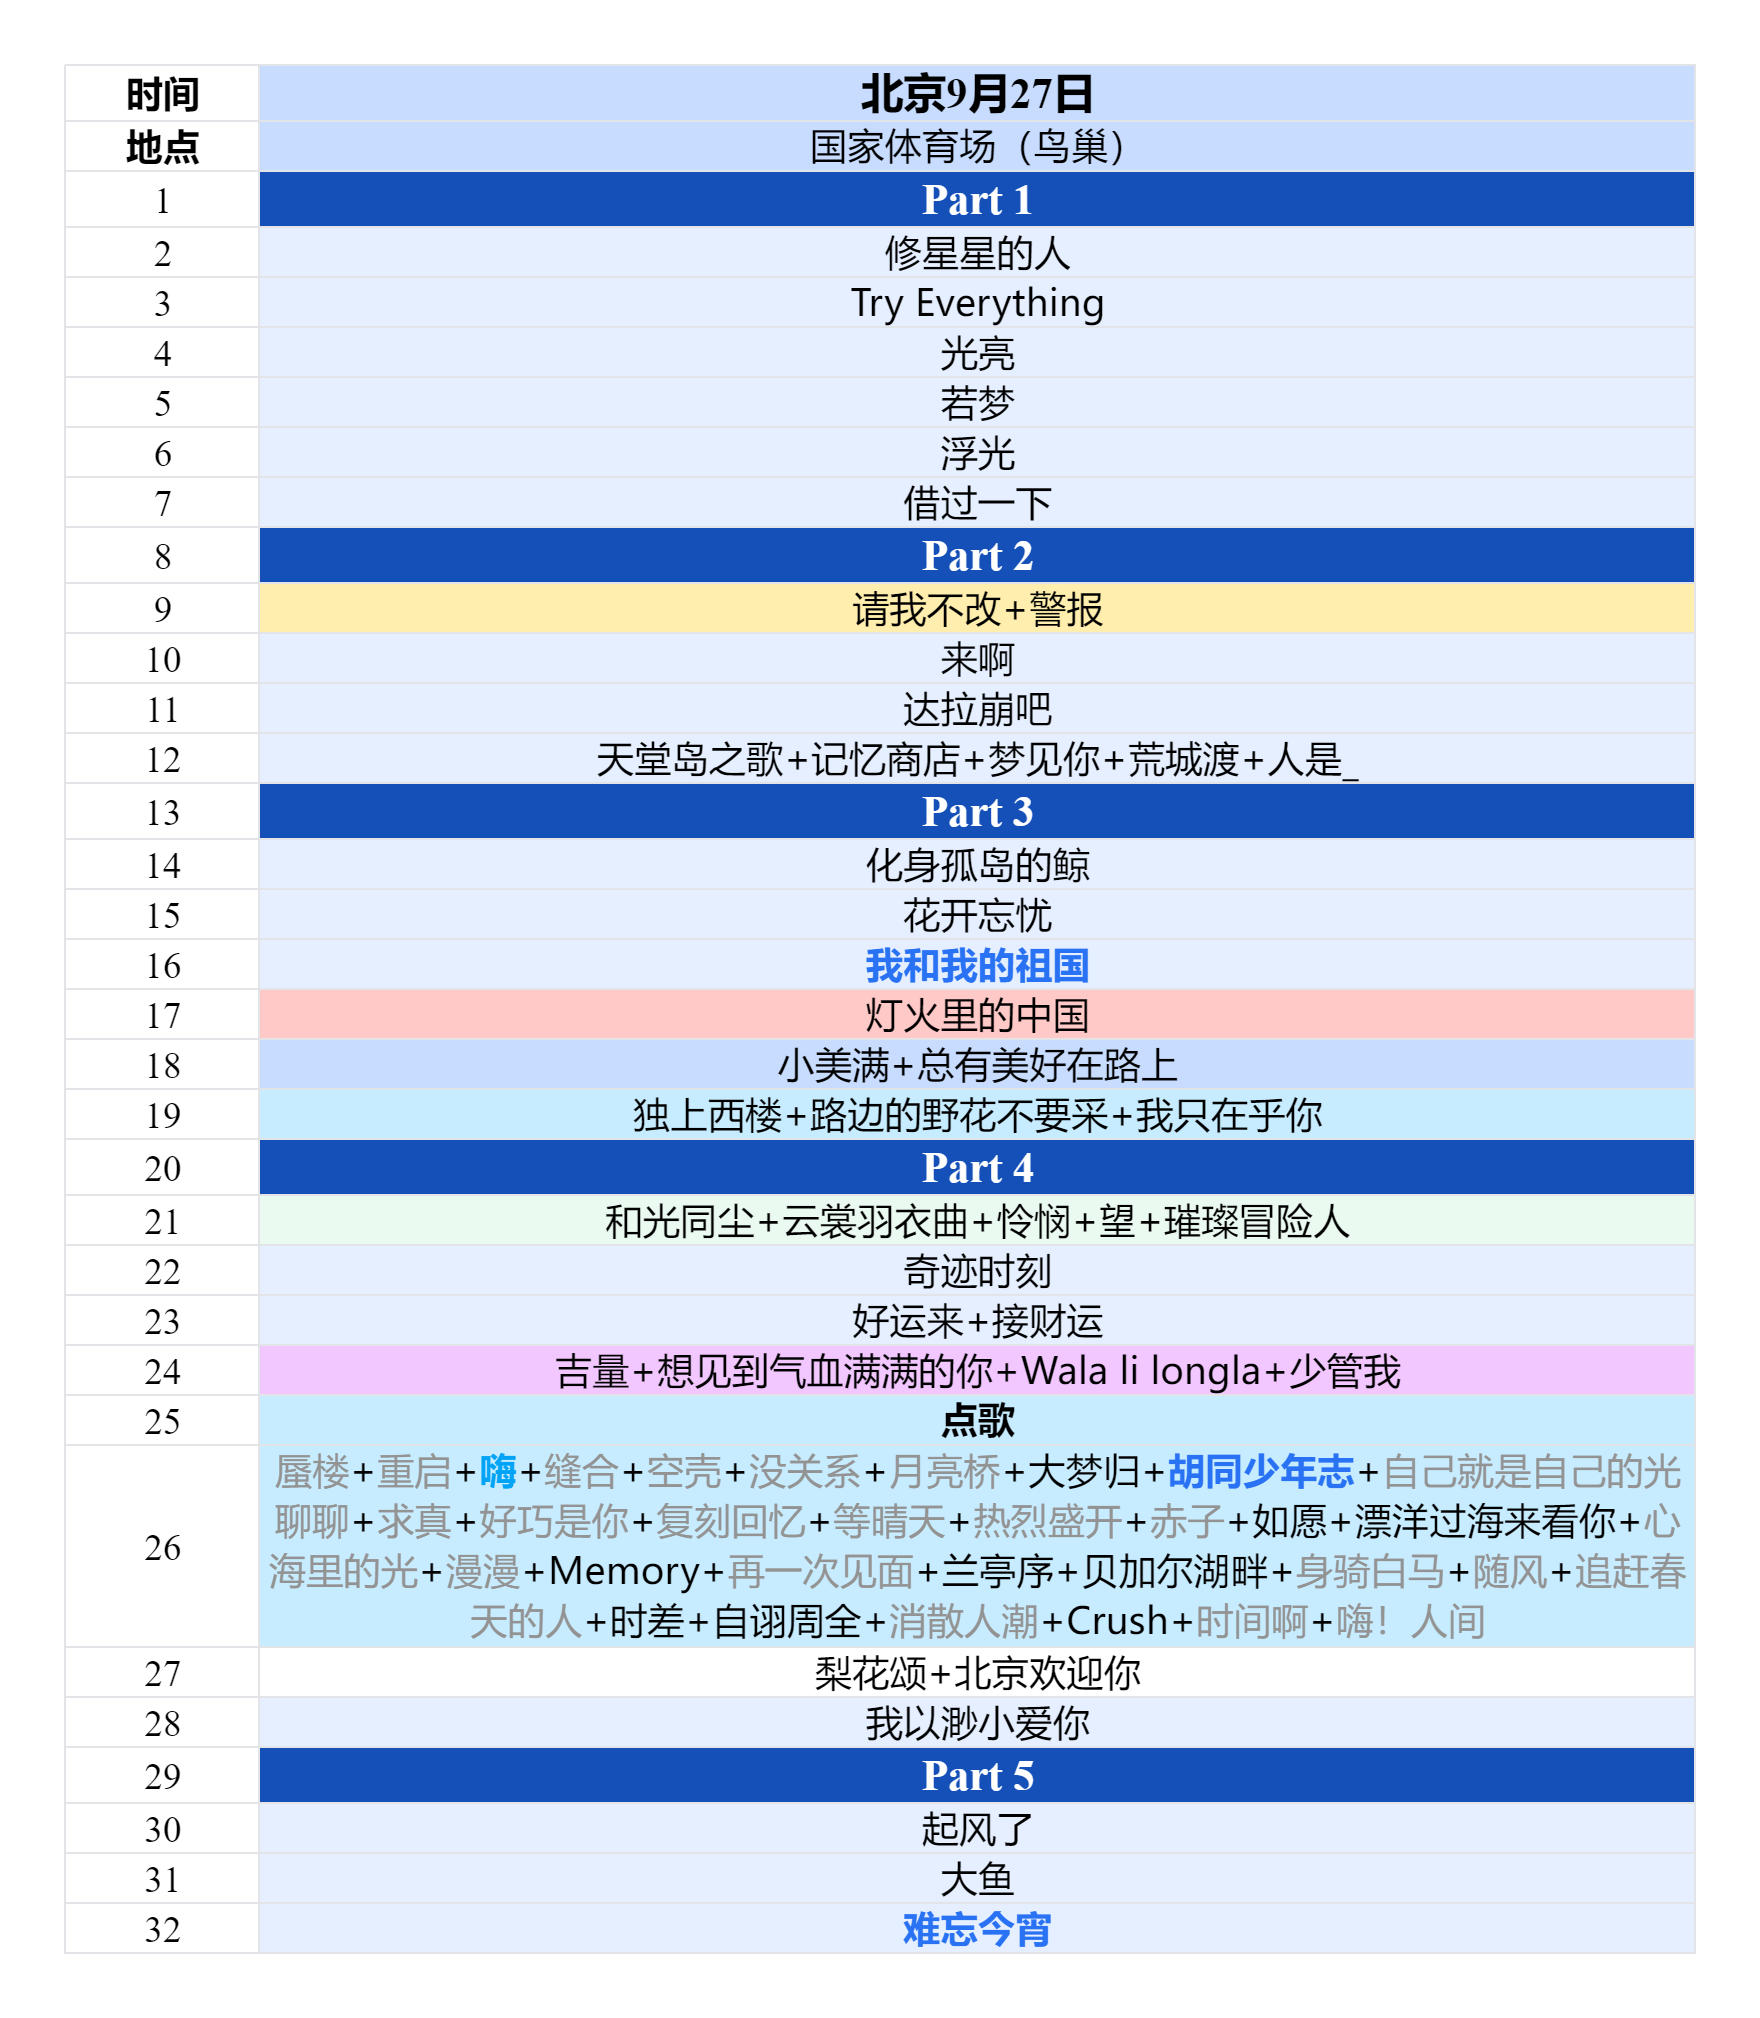
\includegraphics[width=280pt]{img/playlists/BeiJing-20260927} 

}

\caption{2026周深“深深的”巡回演唱会2026.09.27北京场歌单}\label{fig:unnamed-chunk-50}
\end{figure}

\newpage

\section{Part1}\label{BeiJing-20260927-part1}

\hyperref[opening-vcr]{🎥【\textbf{开场VCR}】}（VCR 正文见附录 D，含首句''我们都是来自于一次宇宙大爆炸''。VCR 结束后《修星星的人》前奏直接响起。）

\hyperref[xiu-xing-xing-de-ren]{🎵【\textbf{修星星的人}】}（米：先声合唱：既然这宇宙让我诞生------）（深：是我在故乡的旷野，仰望银河的夏夜；是我在宇宙的风暴，朝着天仓五飘曳；我的孤独我的热烈，源自137亿年前，几粒星尘的蝴蝶；在噬星的幻灭里，为太阳撑一把雨伞；在时间的深海里，给地球道一声晚安〔首句现场听作''是我在呼啸的光年''，待核〕）北京站第三场的朋友们你们好吗！（米：欢呼声）（深：既然这宇宙让我诞生，想必它是要以我为证〔现场听作''上帝的诗由你我完成''，待核〕；我的情感和三十六度的体温，足以暖热即将熄灭的恒星\ldots\ldots 许我以造物的碎屑，重塑文明的边界；许我以渺小的羞怯，挽留物种的毁灭〔第二段主歌现场听作''是我在古老的碎石追溯文明的边界，是我以渺小的修剪挽留无终的\ldots\ldots``，现场版唱词待核〕）（深：既然这宇宙予我重生，想必它是要让我看懂，我的基因和闪闪发光的记忆，足以照亮所有星际的永恒）（高音吟唱）鸟巢的朋友们你们好吗！（米：好------！）

\hyperref[try-everything]{🎵【\textbf{Try Everything}】}既然这个世界让我们诞生，我们就勇敢地 Try Everything 好不好？（米：好------！）（深：I messed up tonight, I lost another fight\ldots\ldots No I won't leave, I wanna try everything / I wanna try even though I could fail）（深：Oh oh oh oh------）（米：Try everything）（深：Oh oh oh oh------）（米：Try everything）（深：Oh oh oh oh------）（米：Try everything）（深：Oh oh oh oh------）（深：Look how far you've come, you filled your heart with love\ldots\ldots I'll keep on making those new mistakes / I'll keep on making them every day / Those new mistakes）全场！（米：Try everything!）再大声！（米：Try everything!）最大声！（米：Try everything!）尖叫声。（米：尖叫声）Every try\ldots{} Every try\ldots〔口播听写待核〕Try everything.（米：欢呼声、掌声）

\hyperref[silver-linings]{🎵【\textbf{光亮}】}哇！大家好，我是歌手周深，谢谢你们来到深深的巡回演唱会！（米：欢呼声、掌声）哇！这是第一次连续三天开演唱会哦。我们真的连续三天相聚在鸟巢了吗？（米：欢呼声）后面的朋友你们好！（米：欢呼声）太开心了。哇，这真的是我完全不敢想的一件事情，但是因为你们的出现，所有一切的一切都发生了。再一次希望你们帮我感谢一下最美好的你们，欢呼声给自己！（米：欢呼声）来到北京要说北京话。让我再听一下你们最大的声音！（米：欢呼声）够噪的。就算算不算地道的一句啊？应该还算的对。〔北京话''够噪的''，听写待核〕大家来北京有没有去吃好吃的呀？（米：有！）也要继续就是去很多很多很漂亮的地方玩好不好？（米：好！）那来到北京啊，就是每一次北京故宫雪景的时候，我的有一首歌中间有个片段会经常出现，你们会唱吗？（米：会！）（深清唱：莫听穿林打叶声）（米合唱：一蓑烟雨任平生〔听作''一烟雨任平生''，已按附录G校正〕）（深清唱：畅音阁里终一叙〔听作''畅饮过离愁应许''，已按附录G校正〕）（米合唱：回首向来萧瑟处，也无风雨也无晴）谢谢你们愿意成为我的光亮，\textbf{\textcolor{red}{我爱你们}}！（米：欢呼声）（深：海上一阵风吹起，白云涌向陆地，季风带走沙粒；四季冷暖的交替，多鲜活的生命，有枯萎的痕迹；是奔跑中突然袭来的风雨，是黑暗中一根火柴燃烧的光明；也许你猜不透未知的宿命，像流星飞翔着它却不知目的；可是啊我却\ldots\ldots 最渺小最微弱最柔软最无畏的你，用尽了全力努力地去回应，再无边再无尽再无解总有一线生机，光亮你自己）（戏曲念白＋唱腔两遍：莫听穿林打叶声，一蓑烟雨任平生；畅音阁里终一叙，六百年一粟，沧海一梦\ldots\ldots 最无畏的你）谢谢你们愿意出现成为我的光亮，谢谢你们！（米：欢呼声）后面的朋友，谢谢你们！（米：合唱高音部分）最无畏的你。

\hyperref[like-a-dream]{🎵【\textbf{若梦}】}跟你们相遇这件事情，美好的跟做梦一样。等一下，能不能用最大的声音一起唱《若梦》啊？（米：能------！）（深：浮生若梦，为欢几何；风摇雨落，此心何处停泊；剑起刀割，却斩不断这因果，看天地之间皆漠漠；尘缘萧索，宿命奈何；日升月落，此生依旧难舍；铁马金戈，也踏不碎这心火；忆前尘旧梦，任岁月消磨）到你们！（米：往事流转，在你眼眸）（深：再大声！）（深：往事流转，在你眼眸）（米：一边遗忘，一边拼凑）（深：如我虔诚，合十双手）（米：如我虔诚，合十双手）最大声！后面呢？全场最大声！（米：往事流转在你眼眸，一边遗忘一边拼凑，如我虔诚合十双手，唯愿你能得到拯救\ldots\ldots 在你眼眸〔逐轮应答〕、一边拼凑、合十双手、得到拯救〔逐轮应答〕）因为你们------你你你你你\ldots\ldots〔对观众的逐个点名致意，听写待核〕

\hyperref[floating-light]{🎵【\textbf{浮光}】}（深：看指尖拨响蝴蝶，扇动一场离别；我推开无声岁月，续梦一页；你我只是打个照面，可曾有过誓约，走进熟悉却陌生的思念）啊\ldots\ldots（深：你的眼眸装满了时间，你的身后拥故事成篇，此生如梦愿细数流年，与你同写沧海桑田；浮光掠影重山彩云间，你的伏线穿越千百年，人生不过恍惚三万天，漫漫人间，留恋流连〔``你的身后永不是终点''``多少重逢也是久别见面''等听写已按附录G校正〕）〔无词吟唱〕（米：欢呼声）〔本段与《若梦》在转写稿中时间戳交错，两曲先后按歌单锚点排序，实际顺序建议人工复核〕

\hyperref[excuse-me]{🎵【\textbf{借过一下}】}（深：少年扬起脸庞，前往他的月亮，人们笑他狂妄，人怎可不一样；白衣过泥潭，怎敢说不染，但凡银两有价，谁能真潇洒；少年爬上城墙，去见他的月亮，破碎几次心脏，得来几句真相；市井或朝堂，四方皆如框，若你生来有刺，磨掉再入场）你们都是对的，他说拜托，让开一下。（深：让我大醉一场，殿堂之上，背闲诗两三章；让我穿白衣裳，过疯人巷，去泥潭捞月光；望大人们见谅，提点的话，我懂也不想装；世人寻黄金乡，我找月亮，何必同往；话谢过，路借过，你是你，我是我）（米：让我大醉一场，殿堂之上，背闲诗两三章；让我穿白衣裳，过风人巷〔``过疯人巷''两读，待核〕，去泥潭捞月光；望大人们见谅，提点的话，我懂也不想装；世人寻黄金乡，我找月亮，何必同往；话谢过，路借过，你是你，我是我）〔合唱逐轮记录〕（深：诚如先生所说，每颗心都有瑕；潇洒不是不怕，是愿付出代价；权衡利弊后，仍守对与错，谢过赐教的话，路借过一下）（米：白日光年外，是故里楼外〔合唱句听写待核〕；知心有所爱，不更改；人间多阴霾，若天真犹在，当披上月光，走夜晚）你们就是我要找的月光，对吗？（米：欢呼声）我找到你了。（米：欢呼声、尖叫声）

\section{Part2}\label{BeiJing-20260927-part2}

\hyperref[robot-vcr]{🎥【\textbf{机器人VCR}】}（VCR 正文见附录 D。VCR 开篇日期句本场听作''2225年5月17日。今天是我被选中执行任务的第200天。系统维持正常运转的73000天''〔数字听写待核〕，其余与附录 D 一致。）

\hyperref[brave-heart]{🎵【\textbf{请我不改}】}（VCR 结束后）鸟巢的朋友们你们好吗？（米：好------！）让我再一次听到你们的声音！（米：啊------！）（深：是谁在我耳边念白，说我不配，我不够好，我必失败；是谁将我双眼遮盖，惩罚我坠入百无一用的黑暗；是谁不断日夜合围向我追来，痛击我最脆弱短板；是谁模糊我的未来，恐惧淹没了期待；绝望已经大军压境，回身却没半个人影，才看清追兵与逃兵，竟都是我自己）〔听写''原因败/我不失败/追逐太过自由的悲哀''等已按附录G校正〕（深：请我不改，我的姿态）（米：嘿！）（深：我的爱我的痛都与生俱来；请我看开，我的存在）（米：嘿！）（深：我的明我的暗都不必躲开；我原谅我自己，捡起遗憾拥抱无奈；我允许我放手，让我勇敢活在现在；我不等待，我不徘徊）（米：嘿！）（深：我的笑我的泪都不再苍白，放肆盛开）到你们！（米：Break out!〔现场应答，或作''Brave heart''，待核〕）Break out!到你们！（米：Break out!）〔与《警报》连唱串烧〕（深：我发送警报声，血红色惊叹号，提醒你自救；被遥控被耗空，快失控快断送，我替你看透；从借用到利用，到享受到滥用，转身就走，他们绝不为你而痛）〔听写''却不算惊叹号惊醒你自救''\,``从剧痛到遗忘到相拥''等已按附录G校正〕（深：请我不改，我的姿态\ldots\ldots 坦荡痛快）（深：我不怕这一生因为你不知还能撑多久；对世界曾宽容，对自己最苛求，顺位排最后；你心口从伤口到决口不开口，笑容始终；我学会痛，为你而痛）〔《警报》尾段唱词按附录G校正〕（米：啊------！呜------！）再一次欢迎大家来到深深的巡回演唱会！（米：啊------！）后面的朋友，让我听到你的声音！（米：啊------！）接下来这首歌，希望你能够跟我一起完成，它叫《来啊》。有人听过吗？（米：有------！）没有听过的我教你们一下很简单的，我就说''Don't tell me''，你们就\ldots\ldots Lie, lie. 好不好？（米：好------！）

\hyperref[jing-bao]{🎵【\textbf{警报}】}〔与《请我不改》连唱串烧〕（深：我发送警报声，血红色惊叹号，提醒你自救；被遥控被耗空，快失控快断送，我替你看透；从借用到利用，到享受到滥用，转身就走，他们绝不为你而痛）〔看台/内场录音下说唱段听写误差大，已按附录G校正，待核〕

\hyperref[lai-a]{🎵【\textbf{来啊}】}（深：Don't tell me）（米：Lie lie lie lie lie lie lie lie）（深：再大声点哟。Don't tell me）（米：Lie lie lie lie lie lie lie lie）（深：这边的朋友。Don't tell me）（米：Lie lie lie lie lie lie lie lie）（深：下次希望我们还可以在更多的见面好不好？〔口播待核〕）（米：好！）（深：那就来呀。我，我怎么就这样呆头呆脑，一不小心落入圈套，沉迷的神魂颠倒，Pass off，这灵魂乱七八糟；我，瞳孔里都是你迷人的笑，越靠越近我越浮躁，神涣散虚无缥缈，Cut stop，躁动太纷纷扰扰；天生的怪胎）（米：Yeah）（深：踌躇着徘徊）（米：Yeah）（深：太嘈杂的时代）（米：Yeah）（深：1v1较量打乱了节拍）（米：Yeah）（深：别气急败坏）（米：Yeah）（深：别着急淘汰）（米：Yeah）（深：一万种防备阻碍，不如就算了，靠过来；将错就错，别拖Let's go，随你操控）（深：Don't tell me）（米：Lie lie lie lie lie lie lie lie）（深：我望眼欲穿你别闪躲）（深：Don't tell me）（米：Lie lie lie lie lie lie lie lie）（深：要爱就爱放纵吧别退缩〔听作''爱就爱吧痛就别退缩''，已按附录G校正〕）（深：Don't tell me）（米：Lie lie lie lie lie lie lie lie）（深：我倾尽所有赴汤蹈火）（深：Don't tell me）（米：Lie lie lie lie lie lie lie lie）（深：敢不敢直视我，Let's fall）〔两轮，合唱逐轮记录〕\textbf{\textcolor{red}{我爱你们}}！（深：Don't tell me）（米：Lie lie lie lie lie lie lie lie）\ldots\ldots（深：你们唱的好好听。Don't tell me）（米：Lie lie lie lie lie lie lie lie）毕竟秋天的风有点凉飕飕，大家要注意添加衣服好不好？（米：好！）

\hyperref[dalabengba]{🎵【\textbf{达拉崩吧}】}那接下来到了我们深深的巡回演唱会的小游戏环节咯。我们可以自行选择你喜欢的颜色，用你的荧光棒给大家十秒钟选择的时间。分别是蓝色、粉色、黄色和绿色。红色是不想跟我互动吗？（米：宝贝！）红色是不是因为你们墙头太多了？（米：没有！）这个每每一个颜色都在闪一下的是什么意思？选择不同的颜色呢代表了你选择了扮演不同的角色。分别蓝色是达拉崩吧，黄色是国王陛下，粉色是公主米娅，那绿色就是恶龙。红色就是\ldots\ldots（米：宝你个头！）突然现在觉得红色感觉是少管我〔玩笑〕。我们商量一下，红色我喊北京，你们喊\ldots\ldots（米：宝贝！）商量是两个人的事情。你们有跟我商量过吗？（米：没有！）没有吧？我们商量一下，我喊北京，你们说\ldots\ldots（米：宝贝！）看来有的时候商量，人和人之间的沟通很难〔口播听写待核〕。我喊北京，你们欢迎你好不好？北京！（米：宝贝！）哇，好整齐啊。哎，达拉崩吧！（米：我最棒！）国王陛下！（米：再说一次！）公主米娅！（米：救我啊！〔听作''要我爱''，按惯例校，待核〕）恶龙！（米：嗷------！）达拉崩吧！（米：我最棒！）国王陛下！（米：再说一次！）公主米娅！（米：救我啊！）恶龙！（米：嗷------！）达拉崩吧！（米：我最棒！）国王陛下！（米：再说一次！）公主米娅！（米：救我啊！）恶龙！（米：嗷嗷！）恶龙！（米：嗷嗷！）恶龙！（米：嗷嗷！）恶龙！（米：嗷嗷！）恶龙！（米：嗷嗷！）恶龙乘以十，走！（米：嗷嗷！嗷嗷！嗷嗷！嗷嗷！嗷嗷！嗷嗷！嗷嗷！嗷嗷！嗷嗷！嗷！）用公主米娅的声音喊恶龙的台词。三二一，走，公主米娅版恶龙！（米：嗷！）哇你们好厉害，你们比我还会唱《达拉崩吧》这首歌。因为我听到有朋友就是前面是''嗷''，后面是''嗷呜''。（米：笑声）那我们一起来回顾一下《达拉崩吧》这个故事吧。（米：好！）（深：很久很久以前，巨龙突然出现，带来灾难，带走了公主又消失不见\ldots\ldots 我说，陛下我叫，达拉崩吧斑得贝迪卜多比鲁翁；再说一次，达拉崩吧斑得贝迪卜多比鲁翁；是不是，达拉崩吧斑得贝迪卜多比鲁翁；对对，达拉崩吧斑得贝迪卜多比鲁翁；英雄达拉崩吧，骑上最快的马\ldots\ldots 巨龙说：我是昆图库塔卡提考特苏瓦西拉松；再来一次，昆图库塔卡提考特苏瓦西拉松；是不是，昆特牌提琴烤蛋挞苏打马拉松；不对是，昆图库塔卡提考特苏瓦西拉松；于是，达拉崩吧斑得贝迪卜多比鲁翁，砍向昆图库塔卡提考特苏瓦西拉松；然后昆图库塔卡提考特苏瓦西拉松，咬了达拉崩吧斑得贝迪卜多比鲁翁；最后达拉崩吧斑得贝迪卜多比鲁翁，他战胜了昆图库塔卡提考特苏瓦西拉松，救出了公主米娅莫拉苏娜丹妮谢莉红，回到了蒙达鲁克硫斯伯古比奇巴勒城）达拉崩吧！（米：我最棒！）国王陛下！（米：再说一次！）公主米娅！（米：救我啊！）恶龙！（米：嗷嗷！）北京！（米：宝贝！）达拉崩吧！（米：我最棒！）你们真棒。（深：国王听说，达拉崩吧斑得贝迪卜多比鲁翁，他打败了昆图库塔卡提考特苏瓦西拉松，就把公主米娅莫拉苏娜丹妮谢莉红，嫁给了达拉崩吧斑得贝迪卜多比鲁翁；啦啦，达拉崩吧公主米娅，幸福得像个童话，他们生下一个孩子，也在天天渐渐长大；为了避免以后麻烦，孩子称作王浩然，他的全名十分难念，我不想念一遍〔附录G作''要念你来念吧''，现场改词待核〕）求你们了。求你们了好不好？（米：好------！）北京！（米：宝贝------！）我都这么卑微了吗？〔玩笑〕达拉崩吧！（米：我最棒！）的全名是？（米：达拉崩吧斑得贝迪卜多比鲁翁！）阿木的全名是？（米：〔观众齐答，听写不清，待核〕）（米：宝贝！）〔``阿木''环节应答内容听写待核〕（高音吟唱）尖叫声！

在前年我发了一张专辑，专辑的名字叫做《反深代词》。说的是在两百年后的世界有这样一个世界叫做反深代词，周深一共有十二个不同的情绪碎片，如果你在听这张专辑，你发现某首歌跟你的经历、跟你的那个感想、跟你的情绪如果是一模一样的话，那证明我们在两百年后的反深代词这个世界彼此相互拥抱安慰了。所以求求大家去听一下这张专辑好不好？（米：好------！）也在今年的这张专辑的实体专辑终于跟大家见面啦。谢谢你们，谢谢大家愿意来跟我们一起走进反深代词这个世界。那如果不知道这张专辑的，求求你去线上也去听一下好不好？也可以听到哦。谢谢大家。（米：好------！）后面的朋友有听到吗？（米：有------！）北京！（米：宝贝------！）很明显上一个问题没有很多人听到。〔玩笑〕那让我们来看一下，在反深代词，就是他有一次走进了蜃楼里，里面发生了什么样的故事，好不好？（米：好------！）

〔蜃楼VCR〕（一、二、三、四、五、六、七、八、九、十\ldots\ldots〔数字倒数声，伴随机械音效；本段与前场不同，附录D未收录，建议补录；完整文字待核〕）

\hyperref[haven-song]{🎵【\textbf{天堂岛之歌}】}（深：叮咚，我有一个秘密，悄悄告诉你，欢迎你来到天堂入口；叮咚，有人在按门铃，是谁在外面？把恶作剧当一种游戏〔听作''是谁在问也''，已按附录G校正〕；听那谁在哭泣，看那谁在窃窃私语，窗外有双眼睛，它在时刻注视着你；叮咚，有人在看你的过去\ldots\ldots 叮咚，有人在看你的未来〔``看你的未来''为现场演唱变体，附录G作''看你的秘密''，待核〕）生米们，你在哪？（米：在这------！〔应答听写待核〕）听过歌手唱歌的朋友，你在哪？（米：在这------！〔应答听写待核〕）（米：有个人从远方来，来自很古老的年代；亲爱的我很抱歉，不说了没有了被替代〔观众合唱段，或为《记忆商店》相关曲目，听写待核〕）〔接记忆商店前互动小剧〕又是哪个在玩花里胡哨的东西掉了一个地球？地球。掉了一个气球的舞者。你心虚吗？你不觉得你有一只手空着？这是不是你存放的一段记忆？记忆。噢，想起来了。这里是反，有人在笑我的演技。重新来。你不觉得你有一只手有点空吗？你是说\ldots\ldots 不要笑我。你是说这个气球里装了一段记忆？记忆？哦！这是《反深代词》当中的''记忆商店''对不对？（米：对！）我在梦里梦到过相同的场景，这是深深的巡回演唱会，对不对？（米：对！）但是跟我梦见的当中不太一样。我梦里好像周深没有连续开过三场演唱会。（米：哇！）而且这可是\ldots\ldots（米：鸟巢！）梦里也没有那么多花里胡哨的东西。哦我知道了。你感觉让我一直拿着哎。我知道，就我们拥有这颗米子心，我们就可以唤醒我们最喜欢的那段回忆，对不对？（米：对！）一起来看一下吧。

\hyperref[the-memory-store]{🎵【\textbf{记忆商店}】}〔唱段听写不清，唱词见附录G《记忆商店》，待人工补录〕

\hyperref[meng-jian-ni]{🎵【\textbf{梦见你}】}（深：看着眼前还年少的你，恍如流年从未淌过去；时光飞逝就算我已经老去，你却仍有着初见时那双清澈的眼睛；当再一次听你唤出我姓名，我已将一生都历尽，明白有些事情早注定；我们都站在时间的河里，离别是相遇的倒影；从初吻后的那天起，就有了再见的伏笔〔现场听作''从触碰后的那天起''，待核〕；我望着你远去的背影，渐行渐远直到看不清；时间会改变一切，却再也无法改变你；若多年后还能够有幸，与你重逢在另一场梦境〔现场听作''凌晨梦境''，待核〕，但愿那时你在人海里，仍将我一眼认清）〔唱词已按附录G校正〕（米：不说了没有了没关系的〔合唱句，听写待核〕×2轮）那就都这样吧，那就祝今天生日的朋友\ldots\ldots（米：生日快乐！）祝昨天或者是前几天生日的朋友\ldots\ldots（米：生日快乐！）祝明天或者跟我一样过几天再过生日的朋友\ldots\ldots（米：生日快乐！）哇你们这一群黑竹荪，也跟太阳变得谄媚。〔``黑竹荪''梗，句意听写待核〕过生日送我的气球对不对？这个寓意是扎心吗？〔``扎心''与气球谐音玩笑〕捏爆它。捏爆这个不捏爆这个。哦，我想想啊，哎呀，你都送我生日祝福了，我怎么肯定会很好的对它，对不对？（米：对！）那就用膝盖捏爆这个。然后用耳朵或者肩膀夹爆这个。加油，大家鼓励他。小心小心，不行不行，这样好像耳朵不太行。那你就嗯用这儿吧。〔气球互动，动作提示听写待核〕这个我们就先不扎心了吧。祝每一个人无论哪一天，都生日快乐！（米：周深生日快乐！）什么？（米：生日快\ldots\ldots〔口播听写不清〕）

\hyperref[huang-cheng-du]{🎵【\textbf{荒城渡}】}你这样让我怎么唱接下来这首很感伤的歌？夜色中寻觅过\ldots\ldots 我的笑嘻嘻，重来。〔被生日应答逗笑，口播听写待核〕（深：夜色中寻觅过，当往事困住我，也盼心中生出一点萤火；孤城的传说有谁来过，将因果赠与我〔听作''将因果都湮没''，已按附录G校正〕；我在等这因果，渡魂渡魄渡我〔现场听作''渡我渡我渡我''〕；纵然已是执着难舍，断了这心魔可原谅我，宿命中获得这解脱）祝你们生日快乐！〔歌中现挂〕（深：眼中拂尘，手中残魂，那故事斑驳荒城〔听作''黄泉下''，已按附录G校正〕；修炼天真，拨开心门，握一颗糖暖这孤身颠簸〔听作''捧一颗烫暖这孤身''，已按附录G校正〕）（米：无数的没有了没人记得〔合唱句，或作''不朽的没有了没人记得''，听写待核〕×2轮）（高音吟唱）

\hyperref[Humans_are_]{🎵【\textbf{人是\_}】}（深：未知摊开棋局，舍弃昨日才可破〔现场听作''舍弃昨日再割破''，待核〕；再见了我的月光我的蓝我的爱；钢铁的巨兽在轰鸣，我们拒绝走入夜晚；破碎是新生的约定，我便愿为尘埃；让死亡觊觎我，让恐惧亲吻我，来摧毁我深爱的一切，可仍夺不走我的选择；弹指间湮灭我，但命运打不败活着；让生命如剧烈的烟火，璀璨熄灭前也将点亮，孩童的双眸；若巨浪已淹没了来路，我是帆亦是舟；是微渺的希望，我们依然前行，没有光指引）〔已按附录G校正〕（深：开始的卑微的勇敢的痛的我〔与附录G''让时空消亡我，你无需记得我''对应段听写差异大，待核〕\ldots\ldots 是微茫中高歌的族类，生命像烟火那就点亮，孩童的双眸，未来的瞳孔）在遇到你们之前我也认为\ldots\ldots 也许我们失去的，过去的美好的记忆才是最好的。但是因为听到了你们大声的陪我一起唱歌，用力的奔向我来跟我们相遇，我才明白我们现在拥有的每一分每一秒才是最宝贵的。你说对吗？（米：对！）（米：合唱：不朽的，永恒的，我们记得〔或作''无数的没有了没人记得''，听写待核〕×4轮）\textbf{\textcolor{red}{我爱你们}}！（米：欢呼声、尖叫声）

\section{Part3}\label{BeiJing-20260927-part3}

\hyperref[music-animations-vcr]{🎥【\textbf{音乐动画VCR}】}（VCR 正文见附录 D，本段为纯音乐动画，无旁白歌词。VCR 前后为纯音乐过场。）

\hyperref[The-whale-who-became-an-island]{🎵【\textbf{化身孤岛的鲸}】}因为知道要跟你相见，于是我出发啦。〔过门导语〕（米：欢呼声、尖叫声）（深：我是只化身孤岛的蓝鲸，有着最巨大的身影，鱼虾在身侧穿行，也有飞鸟在背上停；我路过太多太美的奇景，如同伊甸般的仙境，而大海太平太静，多少故事无人倾听；我爱地中海的天晴，爱西伯利亚的雪景，爱万丈高空的鹰，爱肚皮下的藻荇，我在尽心尽力地多情，直到那一天）最大声！（米：你的衣衫破旧，而歌声却温柔，陪我漫无目的地四处漂流）（深：我的背脊如荒丘，而你却微笑摆首，把它当成整个宇宙）（米：你与太阳挥手，也同海鸥问候，陪我爱天爱地的四处风流；只是遗憾你终究，无法躺在我胸口，欣赏夜空最辽阔的不朽，把星子放入眸）（深：我是只化身孤岛的蓝鲸\ldots\ldots 我有着太冷太清的天性，对天上的她动过情，而云朵太远太轻，辗转之后各安天命；我未入过繁华之境，未听过喧嚣的声音，未见过太多生灵，未有过滚烫心情，所以也未觉大洋正中有多么安静）（深：你的指尖轻柔，抚摸过我所有风浪冲撞出的丑陋疮口；你眼中有春与秋，胜过我见过爱过的一切山川与河流；曾以为我肩头是那么的宽厚，足够撑起海底那座琼楼，而在你到来之后，它显得如此清瘦，我想给你能奔跑的岸头）（米：没有墙头！〔应答提前，接墙头梗〕）你们到底有\ldots\ldots（米：没有！）多少个墙头？（米：没有墙头！）大概意思介绍一下，就是我问，我问我的生米啊，就问你们喜欢哪个歌手呀？他们会说\ldots\ldots（米：周深！）我就会问他们，你们还喜欢哪个歌手啊？他们会说\ldots\ldots（米：没有！）他们会说没有，会说周深。其实哎呦，他们喜欢很多歌手的啊。那我就非常非常真的是非常不礼貌，把其他的歌手的外号吧称为''墙头''，所以我问他们，你们到底有多少个墙头？（米：没有！）但是你们要好好照顾好自己，因为你们是我的过往和往后。〔或作''国王和王后''，按1107/1108场惯例待核〕北京的朋友们你们好，我们来北京看你们了哟。你有好好照顾好自己吗？（米：有！）一定要做到好不好？（米：好！）

\hyperref[Blossoms-that-forget-sorrow]{🎵【\textbf{花开忘忧}】}（深：巷子口买了花，穿过沿街红墙青瓦，夕阳慢慢亲吻着我的白发；推开旧木门回到家；把时光都炖香，而你只是笑不说话；一件遗憾的事就喝一碗汤；庭院深深秋叶飘落；我们苍老的时候就回到小时候，采青梅用来酿酒你不许偷着喝；穿朴素的衣裳牵着那衣袖，捡了小猫名为苍狗，我们睡去的时候像孩子无忧愁；反正也很难上锁这岁月如小偷，若记忆被偷走了忘了我的爱，我会说------）说什么？（米：你好啊！）你们好吗？（米：好------！）（深：这是给你的花，花的名字叫忘忧草，它说时光汹涌如水上烟波，别走远了一起回家）我们一起回家好不好？（米：好------！）（高音吟唱）北京的朋友你们好！我们一起唱吧！（深、米：我们苍老的时候就回到小时候\ldots\ldots 岁月如小偷，若记忆被偷走了忘了我的爱，我会说你好啊）〔到你们！逐轮合唱记录〕（米：离开的人啊，请帮我相爱到剧终〔合唱句，见附录G〕）（高音吟唱）（深：忘忧草开着花，你在月光下不说话，一件遗憾的事就喝一杯茶，庭院深深秋叶飘落）在我们的人生当中，一定有那么一个非常非常重要的人。也住着那一份遗憾，再没有机会见到他。但是我相信，只要我们的思念喊得越大声，他一定听得到。你说，对吗？（米：对------！）所以一定要好好照顾好自己，因为他也一定感受得到。你们说，对吗？（米：对------！）

\hyperref[wo-ai-ni-zhong-guo]{🎵【\textbf{我和我的祖国}】}也很厉害哦。那今天这首歌，我也想听到你们最大的合唱声音。因为有了你们，这一切将会变得越来越好。我和我的祖国！（米：欢呼声）提前祝大家国庆节快乐！大声唱出来好吗？（米：好！）（深：我和我的祖国，一刻也不能分割；无论我走到哪里，都流出一首赞歌）（米：我歌唱每一座高山，我歌唱每一条河）（深：袅袅炊烟，小小村落，路上一道辙。全场！我最亲爱的祖国，我永远紧依着你的心窝，你用你那母亲的脉搏和我诉说）谢谢你们的出现！（米：欢呼声、掌声）一定要好好的去成为自己，好不好？（米：好！）祝我们和我们亲爱的祖国越来越好，好不好？（米：好！）（深：我的祖国和我，像海和浪花一朵；浪是那海的赤子，海是那浪的依托。大声唱！每当大海在微笑，我就是笑的旋涡；我分担着海的忧愁，分享海的欢乐；大声！我最亲爱的祖国，你是大海永不干涸，永远给我碧浪清波，心中的歌。再来！后面的朋友！啦啦啦啦啦啦\ldots\ldots 永远给我碧浪清波，心中的歌）〔多轮合唱逐轮记录；本曲伴随大屏伴奏演唱〕

\hyperref[deng-huo-li-de-zhong-guo]{🎵【\textbf{灯火里的中国}】}你们唱的真好听。灯火里的中国美不美？（米：美！）那也是因为你的出现，它才那么美，也会越来越美，对不对？（米：对！）（深：都市的街巷已灯影婆娑，社区暖暖流淌的欢乐；远山的村落火苗闪烁，渐渐明亮小康的思索）等一下跟我一起大声唱好不好？（米：好！）北京！（米：宝贝！〔惯性应答，笑点〕）（深：归港的船帆从灯塔掠过，追梦脚步月下交错；广场焰火在节日诉说，星空升腾时代的巍峨）到你们！（米：灯火里的中国，青春婀娜）再大声！后面的朋友！（米：灯火里的中国，胸怀辽阔）（米：灯火漫卷的万里山河，初心换回了百年承诺）最大声！（米：灯火里的中国，青春婀娜；灯火里的中国，胸怀辽阔；灯火灿烂的中国梦，灯火荡漾着心中的歌）〔合唱逐轮记录〕（高音吟唱）

\hyperref[simple-bliss]{🎵【\textbf{小美满}】}那这一首，能跟我一起大合唱吗？（米：能！）因为你的出现，我收获了好多好多小美满。谢谢你！（米：谢谢周深！）（深：没什么大愿望）唱！（米：没有什么事要赶）（深：看见路口红灯一直闪，它像眨眼的小太阳；乌云还挺大胆，顶在头上吹不散，我抓在手里捏成棉花糖，什么烦恼不能忘；既然是路一定有转弯，哪个风景都漂亮，揉揉疲惫的眼睛停下来看一看，美好简单）全场一起！（米：你看小狗在叫树叶会笑风声在呢喃，不如好好欣赏一秒迷迷糊糊的浪漫；只要一觉醒来床单洒满阳光的温暖，不去想不必想不用急急忙忙说一个答案）谢谢你们！因为你们出现，我好幸福呀！（深：笑一笑就灿烂）唱！（米：唱一句歌就舒展）（深：收集一点一滴小美满，都是幸福的花样）后面的朋友，前面的朋友一起来！（米：你看小狗在叫树叶会笑风声在呢喃\ldots\ldots 不去想不必想不用急急忙忙说一个答案）大声唱！〔多轮合唱逐轮记录〕

（许愿环节）让我们一起在小美满这首歌当中许愿吧好不好？（米：好！）像我这样哦，我先做个示范。闭上眼睛，想好你的愿望。我会倒数三、二、一，然后睁开眼睛，我们的愿望就会出现在这棵许愿树上。现场无论什么年龄段，无论什么职业，请相信美好的力量，请相信相信的力量，请相信你们的力量。想一想你最想要许的愿望吧。闭上眼睛，想一想生日的时候第一个蹦出来的愿望是什么呢？想一想你一直想要实现的愿望是什么呢？哦对了，小美满的愿望有一个要求，你只能够许关于自己的愿望。想一想你是不是很久很久一直在忙碌，但是却忘记看见自己了呢？想一想你是不是很久没有拥抱过自己？有没有跟自己说一声，你辛苦了，你真的真的很棒，你真的很值得被好好爱着。三、二、一，睁开眼睛！（米：你愿相信什么就把世界看成什么样，偶尔难题加点重量越要轻轻地旋转，所以无论如何记得保管小小的光环；笑就好哭也好今天就是明天最好的陪伴，笑就好哭也好自己就是自己最好的陪伴）你们就是就是最好的陪伴。谢谢你们！（米：谢谢周深！）谢谢你们让这一切发生。因为你们的出现，我才看见\ldots\ldots{}

\hyperref[zong-you-mei-hao-zai-lu-shang]{🎵【\textbf{总有美好在路上}】}（深：花在开云在飘笑容在脸上，我们向前方一路向阳）亲爱的你\ldots\ldots（米：抬头洒满阳光看一看太阳〔合唱句，已按附录G校正〕）（深：让风轻轻\ldots\ldots）（米：吹拂你的脸庞）（深：今天过去\ldots\ldots）（米：要到明天看看天气会怎样）（深：萤火晴朗故事都慢慢讲〔或作''阴或晴朗''，已按附录G校正〕）抬头发现你们就是\ldots\ldots 宝贝！〔改口玩笑〕（米：欢呼声、尖叫声 宝贝！宝贝！）说实话有点油腻。（米：笑声、起哄声）但你们玩得开心吗？（米：开心！）谢谢你们让我成为歌手周深。我也会一直好好努力，成为像我一直以来非常非常喜欢的一位歌手邓丽君女士那样的歌手，用好多好多首歌去存放你们的美好回忆好不好？（米：好！）不过等下的歌里面有你们会唱的，那就大声跟我一起唱好不好？（米：好！）

🎵【\textbf{邓丽君组曲}】

\hyperref[du-shang-xi-lou]{🎵【\textbf{独上西楼}】}（观众：宝贝！）（深：宝你个头。〔应答〕）（深：无言\ldots\ldots 真的无言。〔玩笑〕无言独上西楼，月如钩；寂寞梧桐，深院锁清秋。剪不断理还乱，是离愁，别是一般滋味在心头。剪不断理还乱，是离愁，别是一般滋味在心头。剪不断理还乱，是离愁，别是一般滋味在心头）

\hyperref[donot-pick-the-roadside-flowers]{🎵【\textbf{路边的野花不要采}】}这首歌会唱吗？（米：会！）让我听到你们的声音！（深：送你送到小村外）（米：有句话儿要交代）（深：虽说已经是百花开）那些墙头多的男人听好了〔口播听写待核〕，路边的野花。它怎么了？（米：不要采！）大声唱！（深：记着我的情，记着我的爱）（米：记着有我天天在等待〔合唱句，已按附录G校正〕）（深：我在等着你回来，千万不要把我来忘怀）（米：千万不要把我来忘怀）〔合唱逐轮记录〕你们会忘了我吗？（米：不会！）我绝对不会忘了你们。因为我时常在想，如果没有遇见你们，我现在在干什么呢？

\hyperref[I-only-care-about-you]{🎵【\textbf{我只在乎你}】}（深：如果没有遇见你，我将会是在哪里；日子过得怎么样，人生是否要珍惜）（米：也许认识某一人，过着平凡的日子；不知道会不会，也有爱情甜如蜜）（深：任时光匆匆流去，我只在乎你；心甘情愿感染你的气息；人生几何能够得到知己，失去生命的力量也不可惜；所以我求求你，别让我离开你，除了你我不能感到一丝丝情意）全场大合唱！（深、米：任时光匆匆流去，我只在乎你）谢谢你们！（深、米：心甘情愿感染你的气息；人生几何能够得到知己，失去生命的力量也不可惜；所以我求求你，别让我离开你）你们！（米：除了你我不能感到一丝丝情意）（深：除了你我不能感到一丝丝情意）你们会忘了我吗？（米：不会！）我只在乎你！

\section{Part4}\label{BeiJing-20260927-part4}

\hyperref[mask-vcr]{🎥【\textbf{面具VCR}】}（VCR 正文见附录 D。开篇日期行本场为''2026年9月27日，北京''，其余与附录 D 一致；VCR 中''你的声音好像有点不一样哦，我觉得\ldots\ldots{}``处，现场观众接话''很好听！``，结尾''你说，对吗？``后本场口播为''你们会跟我一起大声唱歌，你们说，对吗？``。）

（米：对！）〔回应 VCR 结尾''你说，对吗？``〕没听到哦。你说，对吗？（米：对！）你们会跟我一起大声唱歌，你们说，对吗？（米：对！）

\hyperref[stay-with-light]{🎵【\textbf{和光同尘}】}（深：和你一起歌，和你一起合，月落星沉，日出东海。你们！）（米：和你走过，理想的大河，从容地，沸腾着）〔合唱句已按附录G校正〕（深：你看那盛放的花，来自期盼的种子；你看那丰硕果实，来自耕耘的浪漫；宽广的大河，来自八方汇聚的小溪；奔腾向前的大江，来自高山的哺育）（深：和光同行，跌跌撞撞的摸索；和光同舞，奋不顾身的坎坷；和光同尘，不为盛名而来〔现场听作''不为生命而来''，已按附录G校正〕，不为低谷而去；和光同尘，为你而来，有你，不再〔或作''有你，我在''，按附录G待核〕）

\hyperref[Song-of-the-cloud-dress]{🎵【\textbf{云裳羽衣曲}】}我们的缘分一定不会太浅，因为我的名字叫\ldots\ldots（米：周深！）因为我们巡回演唱会的名字叫\ldots\ldots（米：9.29赫兹！）〔观众以2024巡演名''9.29赫兹''应答，口播与应答待核〕大声陪我一起唱吧！（深：故事鲜艳）（米：而缘分却太浅）（深：我的爱恋）（米：竟如此的明显）（深：我不停地默念，想牢记你的容颜；故事鲜艳，而结局却搁浅，这些年你又在那座红尘之间，幻化成哪张脸）〔``这些年你又在那座红尘之间''或作''这些年你又在哪座红尘之间''，待核〕（深：你轻落指尖，月下拨弄琴弦〔听作''云袖之间月下拨弄琴弦''，已按附录G校正〕，一曲云裳羽衣恋〔听作''一曲吟唱月夜难眠''，已按附录G校正〕，人世间，漫天飞舞着思念）〔结尾另有''风会化作山间的风雨，在你身边''等唱句听写不清，待核〕

\hyperref[lian-min]{🎵【\textbf{怜悯}】}（深：我要比你）（米：来的勇猛，去的彻底，光明，愿你有浩海的动力〔现场应和句，听写待核〕）（深：我要带着）（米：来时的初心，走的无悔，无惧，无畏，华丽转身〔现场应和句，听写待核〕）太好听了！〔口播〕〔另有''我要望着远近疏林\ldots\ldots 天地同归寂''等唱句听写不清，待核〕〔唱段听写不清，唱词见附录G《怜悯》，待人工补录〕我们不要祈求怜悯，我们不要生病，我们都值得被好好的爱着，你们说对不对？（米：对！）

\hyperref[Expectation]{🎵【\textbf{望}】}我们总会绕啊绕（米：绕啊绕）（米：绕几千里路也望向归途）（深：乘着风，想念吹拂，游夜空漂浮，抓一颗流星做礼物，愿你幸福。手中线，绕啊绕）（米：绕啊绕）（米：绕几千日夜也望向归途〔听作''绕几千年日夜也想归途''，已按附录G校正〕）（深：燕归巢，迁徙之路，参与者无数，待到烟火照夜白时，准备庆祝。我们心有所住。再大声！）我们总会绕啊绕（米：绕啊绕）（米：绕几千里路也望向归途）我们终于见面啦！〔口播〕（深：抓一颗流星祝福你要幸福；手中线绕啊绕，绕啊绕，绕几千日夜也望向归途；燕归巢，迁徙之路，参与者无数，待到烟火照夜白时准备庆祝，我们心有所住）谢谢你们！（米：谢谢！）

\hyperref[adventurers]{🎵【\textbf{璀璨冒险人}】}璀璨冒险人们，你们准备好了吗？我们一起向前冲吧，好不好？（深：他们说要越过前方风沙必须低着头，他们说要绕过蜿蜒的河才能往前走；他们说烫要放手，太阳要换个路口，如果得不到谁的认同那就不算拥有；没人能够决定谁的一生应该怎么活）你们！（米：欢呼）（深：没人能够定义谁的天空是什么颜色）再大声！（深：没人未梦就先懂〔听作''没人能够就是梦''，已按附录G校正〕，只是单纯相信着，背向光的英雄，每张轮廓，出自平凡的沉默。你们都是我的英雄！）（米：哇！）（深：沿途一身泥泞跌撞的是我，忍痛缓行不回头的也是我〔听作''忍痛换醒不回头''，已按附录G校正〕；就让一路曲折，每一道伤口，洗净我的脆弱）（米：原来咽回去的泪，才能淹没了脆弱；你发誓更勇敢一生与梦相拥〔``一路相拥''等听写已按附录G校正〕；还想要继续吗？要逆风不退啊〔听作''高飞从不退让''，已按附录G校正〕，让痛苦住进你眼眸〔听作''感动不止于眼眶''，已按附录G校正〕；别怕未来的模样，辜负曾经的凝望，有多少理想就有多少次传唱〔听作''多少次战场''，已按附录G校正〕；那沿途的风浪，也不过就这样，这一路光景有你在身旁；要炙热啊，要不枉啊，要勇往啊；起风了，呼唤了，你还在等什么；挥手了，再见了，别不舍回头啊，向心中的梦啊，去追吧）〔Rap段已按附录G校正〕（深：要多少伤痕才算活过，愿你记得，愿你懂我，不惧脆弱）〔``愿你哭过''听作''愿你懂我''，已按附录G校正；现场重复''不惧脆弱''多轮〕谢谢你们！（米：谢谢周深！）因为你们的出现，我们真的做到了！（米：欢呼声）十二年前的周深也不敢想自己有机会能够开演唱会，而且是在鸟巢开演唱会。这都是你们创造的奇迹，所以不要小瞧你们自己好吗？（米：好！）请努力地尝试，勇敢地拥抱自己，不要害怕看到自己脆弱的一面。我不知道你现在面对，也许在面对的一些挑战，或是面对着一些自我的一些困境，但是请相信，好好地去看见自己，拥抱自己，做好现在该做的事情，我们一定、一定、一定会到达我们最想去的目的地，对不对？（米：对！）就像你们看见我一样。我们要勇敢向前冲，要无畏，也不惧脆弱。（抽泣声）其实我刚才为什么哭，是因为等下又要变魔术。〔玩笑〕

\hyperref[miracle-moment]{🎵【\textbf{奇迹时刻}】}被你们看见的这一秒，就叫做奇迹时刻。（米：欢呼声）（深：从银河抹去的恒星，穿梭时空的王牌，一个瞬息就能将不思议解开；礼帽会翻出精灵，还是一整片星海，那悬念在左手或右手，Never know；这世界总有太多陆离光怪，以惊喜回应期待，We can dream, we can fly；若相信谁都可以重塑现在，不需要等待，Show time，此刻就无限精彩；I wanna see my way in the starlight，奇迹时刻等你一起来，开启夺目现在；We gonna change the fate never deny，以无数颗渺小的光彩，就能照亮无穷未来）〔听写''唱破过去的封印''\,``魔法会翻出新意''``爱是比翼成片星海''等已按附录G校正；副歌两轮〕你们好吗？（深：这世界总有太多无理光怪〔待核〕\ldots\ldots 无论要去多远的宇宙，Here we go）掌声鼓励我，变魔术！（米：欢呼声）我还需要一点鼓励。（米：欢呼声）【魔术环节】最近周深工作室来了一个新的小朋友，他叫\ldots\ldots 他叫苍狗。〔``捡了小猫名为苍狗''梗〕可不可爱？（米：可爱！）所以呢，听说苍狗想要告诉你们，一定要把你们的钱先留给自己花，好不好？（米：好！）所以他拿出了一个硬币。大家看一下，他是怎么帮大家\ldots\ldots 哎哟哟哟哟哟，错了错了错了。哎哟哟哟哟，错了错了错了。大家有看到吗？这个硬币在这里对不对？大家有看到吗？给我倒数三个数字。三、二、一。怎么会这么安静？重来，没看清是不是？重来一下啊。来，三个数字，三、二、一！（米：欢呼声）他又来啦！大家看一下熟悉的，这里面是四个骰子对不对？特写。〔``四个头子''听写已校〕倒数三个数字，三\ldots\ldots（米：二、一！）（米：欢呼声）等我再看一会小抄，稍等。〔自嘲小抄梗〕假装没看见这个过程。倒数三\ldots\ldots 哇塞，好细节的描述啊。〔口播听写待核〕倒数三个数字！（米：三、二、一！）（米：欢呼声）怎么会多一个？好运来了大家接不接？（米：接！）后面的朋友，好运来了接不接？（米：接！）我的魔术成不成功？（米：成功！）

\hyperref[good-fortune-comes]{🎵【\textbf{好运来}】}（深、米：好运来，祝你好运来，好运带来了喜和爱）在跟我见面之前要提前先照顾好自己好不好？（米：好！）（深、米：叠个千纸鹤再系个红飘带，愿善良的人们天天好运来；你勤劳生活美，你健康春常在，你一生的忙碌为了笑逐颜开；打个中国结，请春风剪个彩，愿祖国的日月年年好运来；你凤舞太平年，你龙腾新时代，你幸福的家园迎来百花盛开）大声唱！（深、米：好运来，祝你好运来，好运带来了喜和爱）大声！（深、米：好运来，我们好运来，迎着好运兴旺发达通四海）北京的朋友，身体健康！接不接？（米：接！）恭喜发财，接不接？（深、米：叠个千纸鹤，再系个红飘带\ldots\ldots 你幸福的家园迎来百花盛开）大声唱！再大声！再一次！〔合唱逐轮记录〕鸟巢的朋友们你们好吗？（米：好------！）所有的幸福和好运来了，等下跟我一起大声的接，好不好？（米：好------！）我喊什么你们跟我一起喊哟。

\hyperref[jie-cai-yun]{🎵【\textbf{接财运}】}我们一起接平安！（米：接平安！）接幸福！（米：接幸福！）接健康！（米：接健康！）接财运！（米：接财运！）恭喜发财接不接？（深、米：接个好运来，接个福气来，接个财神开开心心到我家门来〔``到我家里来''听写已按附录G校正〕；接个财运来，小财大财，我接我接，我接金山银海；好运来，我接着好运在〔后段合唱句听写不清，待核〕\ldots\ldots 嘿！我接个一口袋〔或作''我接满亿口袋''，待核〕）北京的朋友，祝你们恭喜发财！接不接？（米：接------！）老鼠干这个东西到底是怎么流行起来的？〔口播听写待核〕（米：〔听写待核〕）好看吗？（米：不好看！）不好看但是是你们让它流行起来的呀。（米：没有！）〔玩笑〕哦，大家刚才有没有好好的接好运呀？（米：有------！）那我就要坐着我们的小车车来看一下有谁没有好好的接好运咯。（米：哇------！）

\hyperref[ji-liang]{🎵【\textbf{吉量}】}祝大家在马年拥有无量的吉祥。吉量你们会唱吗？（米：会------！）那等一下让我听到你的声音。（米：羲和车上金铃铛〔听作''西河车上叮铃铛''，已按附录G校正〕，叮当叮当）哇！哇我发现我们第三场的朋友们唱的尤其的大声，等一下就让我听到你们的声音好不好？（米：好------！）前面两场唱的也很大声啊对不起啊。〔玩笑〕（深、米：羲和车上金铃铛，叮当叮当）到你们！（米：叮当叮当）（深、米：望舒驾后银尾巴〔听作''老鼠夹后硬尾巴''，已按附录G校正〕，摇摇晃晃）（深、米：弱水岸边唤吉量〔听作''热血连环激亮''，已按附录G校正〕，吉量吉量，叮叮当当，天地叮叮当当）（深、米：九天之上飘来一朵雪花，原来是我那英俊的小马；金色星星在它眼里安家，祝融手持火种编织了它的发〔听作''朱榕树枝火种''，已按附录G校正〕；我的小马一天一天长大，穿过凛冬和最沸腾的夏；衔来西边石头东边的花，马蹄扬起层层层层的云沙〔听作''云霞''，已按附录G校正〕）跟我一起！（深、米：高高山上鸾鸟唱〔听作''高高山上看庙堂''，已按附录G校正〕，叮当叮当）（米：叮当叮当）（深、米：东海浪里搅银汤〔听作''东海浪里找明堂''，已按附录G校正〕，汤汤荡荡）（米：响响当当〔应答听写待核〕）（深、米：建木树下唤吉量〔听作''千古树下换脊梁''，已按附录G校正〕，吉量吉量，叮叮当当，天地叮叮当当）〔观众合唱段逐轮记录；``吉量''多听作''激亮/脊梁/计量''，均已按附录G校正〕（深、米：吉量，我亲爱的小马〔听作''吉量，注定像那颗太阳''，已按附录G校正〕，漫漫长夜你呀，抖一抖脊梁；吉量，当你路过他乡，最绵长的山岗，要挂我的月亮）〔第二段合唱听写与附录G差异较大，待核〕你们好吗？（米：好！）

\hyperref[xiang-jian-dao-qi-xue-man-man-de-ni]{🎵【\textbf{想见到气血满满的你}】}（深：你是谁？你是自己的------）（米：宝贝！）（深：宝贝！〔口播〕（深：有时候感觉自己多珍贵〔听作''要是怕，感觉自己多珍贵''，待核〕，还会有更好的等着你，还有好多梦在飞，还要给自己一个新的机会。要早起早睡，别那么累，做好气血满满的准备〔听作''做好积蓄满满的准备''，已按附录G校正〕；想见到你，灿烂的你，无惧也无畏；别害怕疼痛，别怕眼泪，就让我来陪着你找回，手里有暖，心里有暖，阳光更明媚）注意安全哟，谢谢你们！〔口播〕（深：若再痛再冷再怕的时候，请你一定记得。你们好！我永远会是你停靠的选择〔已按附录G校正〕；唯有梦可贵，勇气可贵，举起热情满满的奖杯；那时的你，灿烂的你，无惧也无畏；无论多少岁，精神百倍，我都会来陪着你找回，手里有暖，心里有暖，阳光的明媚）嘿，你是谁？你是自己的\ldots\ldots（米：宝贝！）这边的朋友你们好吗？（米：好！）这边的朋友你们好吗？（米：好！）在我前天发的专辑《反深代词》当中〔``前天''待核〕有个快乐密码，等一下跟我一起最大声喊出来好不好？（米：好！）拜托你们帮我大声的喊，因为喊得越大声，快乐来得越快哟。教你们哦，Wala li longla！（米：Wala li longla！）Wala li longla！（米：Wala li longla！）全场最大声，Wala li longla！（米：Wala li longla！）

\hyperref[wala-li-longla]{🎵【\textbf{Wala li longla}】}（深：把蜗牛都放大，把汽泡堆成塔，口味自由混搭，用沙砾提炼火花；无所谓章法，无所谓多伟大，一默念就触发〔听作''一默念就出发''，已按附录G校正〕，Wala li longla）〔现场版唱词与附录G差异较大：``终点就一瞬逆转成魔法''``信念会解码整片蒙娜丽莎''``恋爱的花火，玛格丽特''``我可知浪花''``面包和冰是懂的不假''等，待核〕你们好吗？（深：Wala li longla）谢谢你们！谢谢你们出现在这里！（米：谢谢周深！）全场的朋友，我喊什么，你们就喊什么，我们一起喊响这个快乐密码好不好？鸟巢的朋友！Wala！（米：Wala！）Wala li！（米：Wala li！）Wala li long！（米：Wala li long！）Wala li longla！（米：Wala li longla！）Wala！（米：Wala！）Wala li！（米：Wala li！）Wala li long！（米：Wala li long！）Wala li longla！（米：Wala li longla！）〔三轮以上逐轮记录〕（米：Wala li longla!）（深：Wala li longla!）〔交替对喊多轮〕上面的朋友！（米：Wala li longla!）全场！（合：Wala li longla!）（合：管他明天会怎样，心又起了浪。稀里又哗啦。〔现场版唱词，待核〕）（深：没事没事注意安全。）（合：全世界随心听见神秘码〔现场版唱词，待核〕）（深：没事儿。）（合：管他大西瓜还是内向瓜，反正我优雅。〔现场版唱词，待核〕）（深：Wala li longla! 大家注意安全哦。）（合：心里有花吗？〔现场版唱词，待核〕）全场最大声来一遍！（米：Wala li longla!）（深：Woo!）

\hyperref[watch-ur-manners]{🎵【\textbf{少管我}】}哎，那接下来我们还有一个暗号，就是少管我，三二一，嘿！（米：少管我！〔或作''嘿！少管我！``，待核〕）全场最大声，嘿！（米：少管我！）嘿，少管我。会唱的跟我一起哟。（合：嘿，少管我。嘿，少管我。）（深：有什么关系，删掉无聊的理由；把沉重身体传送到热带气候，脑袋放空，去吹海风；用一场远行当做逃离的方舟；做生活困兽不如去浪漫宇宙，烦恼忧愁，全部都抽空）〔''看霓虹灯初上，热闹出窍；给单调的人生换一份曲调；你像游离的流星做信号；掠过无数人生指南的街道；不在乎寻找什么，只经过灵魂的桥''等现场唱词与附录G差异较大，待核〕你们好吗？一起！（深：我想我可以抓住风中飘散的花，不介意坠入水星或是泥巴；跟现在握手拥抱道别出发，别停下；我想我成为阳光、蔷薇、飞鸟、盛夏，或成为昆虫、沙砾、一片雪花，我不在乎）三二一，嘿！（米：少管我！）全场，五四三二一，嘿！（米：少管我！）上面的朋友，嘿！（米：少管我！）三二一，嘿！（米：少管我！）你们好吗？（深：我想我可以\ldots\ldots 别停下）（深：三二一，嘿！）（米：少管我！）（深：唱着这旅途〔或作''将这段旅途''，已按附录G校正〕。嘿！）（米：少管我！）（深：三二一，嘿！）（米：少管我！）（深：唱着这旅途，在这世界的束缚。对你更好，好了五四三二一，全场，嘿！〔口播听写待核〕）（米：少管我！）谢谢你们。（米：谢谢周深！）《少管我》是一首轻松活泼愉快的歌曲，不是让你们去争执或者是去吵架。是想要告诉你啊，在寻找自己的这一条道路上，在你在寻找自己的过程当中，如果出现一些杂音的话，如果在就是在不打扰别人的前提下，就轻轻松松地说一句，嘿！（米：少管我！）只有你才能够找到更好的自己，好不好？（米：好！）哇，刚才转了一圈好开心啊，我又见到你们了，亲爱的朋友们，我们终于见面啦！（米：欢呼声）

【\textbf{点歌环节}】那让我们一起来点歌吧好不好？（米：好！）全场帮我倒数五个数字，五！（米：四！三！二！）耶！停。哇，你们真好。只有你们就是就就对我就是所有的问题都有回答。〔口播听写待核〕你们好吗？（米：好！）你们太好了。Hello，您好。（米：深深宝贝好！）经历过昨天的周深，已经不害怕这两个字了。开玩笑的，宝你个头。请问怎么称呼您？（饼饼：嗯我叫饼饼，曲奇饼的饼。）饼饼，是来自哪里的朋友？（饼饼：呃我老家是安徽，但我小时候就搬去云南昆明。）哦，所以是在云南昆明长大的安徽的朋友。（饼饼：对。）跟我很像，我是在贵州长大的湖南人。（饼饼：我们很有缘分。）是的是的。那安徽会唱黄梅戏吗你？（饼饼：不会。）用安徽话给我们北京的朋友打个招呼好不好？（饼饼：我不会安徽话，但是\ldots\ldots）（深：哦你会云南话。）（饼饼：我跟我朋友学了一句。）（深：学的一句什么？云南话还是安徽话？）（饼饼：云南话。呃\ldots\ldots）（深：你在云南应该生活了很多年对不对？）（饼饼：对。）（深：专门只找了朋友学了一句云南话。）（饼饼：对，专门为今天学的。）（深：在云南说普通话哈。）（饼饼：对。）（深：学\ldots\ldots 好，学了一句什么？）（饼饼：北京欢迎你。）（深：北京\ldots\ldots）（饼饼：欢迎你。）（深：你在贵阳长大，你这个云南话好像不是很标准。〔口播''贵阳''待核，或为口误〕）（饼饼：尽力了。）（深：尽力了，好的，谢谢你。第几次来到北京啊？）（饼饼：呃第二次。）（深：第二次。上一次是来看别人的演唱会吗？）（饼饼：不是，是小时候跟爸爸来逛故宫。）（深：我没有在压力她，我只是在问这个问题而已。你们的眼神让我感觉很可怕哎。没有就好。）（饼饼：没有墙头。）（深：谢谢。哦那你所以你是第一次来看我们演唱会吗？）（饼饼：不是。）（深：哦。）（饼饼：第一次是五月三十一号的重庆。）（深：哇，谢谢你。让我们北京的朋友欢迎我们的饼饼！（米：欢呼声）你也用最热烈的声音感谢我们北京的朋友吧。）（饼饼：谢谢大家！）（深：今天是一个人来的还是跟朋友一起来的？）（饼饼：和全国各地还有海外各地的生米老师们一起来的。）（米：欢呼声）（深：你这句话说完感觉你不是生米老师。〔玩笑〕第一首听到我的歌是哪首歌？）（饼饼：化身孤岛的鲸。）（深：哦，来喽。）（深唱：你的一身破旧〔``你的衣衫破旧''之误唱示范，待核〕）（饼饼唱：而指尖却轻柔）（深：指尖轻柔是做了软化吗这个指甲？〔玩笑〕）（深唱：你的指尖轻柔，而歌声却\ldots\ldots）（深：就这样吧，谢谢你哦。那帮我们点出今天的第一首歌好不好？）（饼饼：点歌之前我有几句话想说。）（深：可以啊，可以用云南话吗？）（饼饼：不可以。）（深：安徽话？）（饼饼：也不可以。）（深：那就北京话吧。）（饼饼：一句话儿。反身代词，深专大门儿。〔口音梗，听写待核〕）（深：我是听懂了的。我没听懂是哪里的话。反身代词？）（饼饼：深专大门儿。）（深：帮我们点出第一首歌吧。）（饼饼：还有几句话，马上很快。）（深：来吧没事。）（饼饼：第二句话是我们很珍惜和深深的每一次相遇，我们也不后悔，对不对？）（米：对！）（饼饼：所以希望深深能够好好照顾自己。）（深：一定会的。大家也要好好照顾好自己好不好？）（米：好！）（深：帮我们点出今天的第一首歌吧。）（饼饼：还有第三句话。）（深：你说你说，哎呦。）（饼饼：请生米老师和我一起预祝深深------）（米：生日快乐！）（深：不要再提醒我了，我知道我即将又要大一岁了。谢谢各位。好啦，谢谢大家的祝福，来帮我们点出今天第一首歌吧。）（饼饼：我想听有Wink和弹舌的《胡同少年志》！）（米：欢呼声）（深：我说我没有一首歌叫有Wink呀。〔玩笑〕谢谢你哦，那在深深的巡回演唱会上留下你灿烂的笑脸好不好？看前面的摄像老师。反身代词，这到底是哪儿的话呀？也不太像是云南话，不是这样讲的嘎。来吧，看前面摄像师，对。哇哦，是不让可可看全这个场景是不是？〔``可可''梗，口播待核〕哎不是啊，不要挡住你\ldots\ldots 你的脸哟，饼饼。对对，来，三二一，耶！哇，这张可以吗？可以啊，谢谢饼饼。谢谢你。谢谢你也点了一首我自己自己的〔口误〕一首歌，也非常我们觉得有一点点北京风格的一首歌啊，《胡同少年志》，希望大家喜欢。（米：欢呼声）有人听过吗？（米：有！）那等下会跟我一起唱吗？（米：会！）荧光棒哦。

\hyperref[hu-tong-shao-nian-zhi]{🎵【\textbf{胡同少年志}】}（深：啊啊啊啊啊\ldots\ldots 拐角的胡同今晚偷偷堆了一点雪；白昼的喧嚣更成卯时二刻的明月〔现场听作''更衬''，待核〕；角楼有灯火彻夜照亮着老街；匆忙是因为我感伤就要道别〔现场听作''我赶上就要道别''，已按附录G校正〕）啊啊啊啊啊\ldots\ldots（深：我眼中百岁的城墙还沐浴着晚霞；城门墩儿老人弹唱着一弦一调，也打动谁吗）三二一！（深：我又不是那个他，一别京城种兰花〔听作''一眼京城种了花''，已按附录G校正〕）（米：古道西风骑着瘦马）（深：万户灯火少离家〔听作''望胡同多少离家''，已按附录G校正〕，背把三弦走天涯〔听作''背把三尺''，已按附录G校正〕）（米：胡同少年立志闯出一番）（深：糖葫芦十颗一串儿〔听作''十个一串''，已按附录G校正〕）（米：糖葫芦十个一串）（深：胡同口捏一个面人儿）（米：胡同口捏一个面人儿）（深：家安在四合小院儿〔听作''叫安在四合小院''，已按附录G校正〕）（米：叫安在四合小院）（深：隔壁还住了个戏班儿，天不亮就练上铜锣儿〔现场听作''隔壁还住了个媳妇儿，天不亮就练声唱歌''，已按附录G校正〕）（深：我眼中百岁的城墙还沐浴着晚霞；城门墩儿老人弹唱着一弦一调，也打动谁吗）会唱的一起！（深：我又不是那个他，一别京城种兰花）（米：古道西风骑着瘦马）（深：万户灯火少离家，背把三弦走天涯）（米：胡同少年立志闯出）啊啊啊啊啊\ldots\ldots 谢谢你们。谢谢大家！（米：谢谢周深！）再帮我倒数五个数字吧。五！（米：四、三、二、一）停。诶？您好。（阿琳：你好，深深宝贝！）（深：过分。宝你个头，请问怎么称呼您？）（阿琳：我叫阿琳。）（深：阿琳？）（阿琳：对。）（深：是来自哪里的阿琳呢？）（阿琳：来自山东的阿琳。）（深：阿梨还是阿琳？）（阿琳：琳琅满目的琳。）（深：你自己回去听一下你这段介绍。琳琅满目。阿琳，你好。）（阿琳：你好，深深。）（深：鲁A济南车。）（阿琳：鲁B青岛的。）（深：好的哟。那第一次听到我的歌是哪首歌呀？）（阿琳：是《大鱼》。）（深：哦，那跟我们唱两句好不好？啊\ldots\ldots）（阿琳：啊\ldots\ldots）（深：挺好的。但是我觉得你\ldots 你的声音很嘹亮，这点我非常喜欢。就是一定要大声的表达自己好不好？阿琳。）（阿琳：好的！深深宝贝！）（深：宝你个头，这声倒是很大声。〔玩笑〕今天是一个人来的吗？）（阿琳：呃，跟我的新晋老公来的。）（深：哎呦！是刚结婚对吧？什么时候结婚的？）（阿琳：八月一号领的证。）（深：哦，我们祝他们幸福美满，来大家也祝你们------）（米：幸福美满！）（深：让他来跟我们打个招呼吧。您好，怎么称呼您？）（盼盼：Hello，深深。）（深：怎么称呼您？你好。）（盼盼：宝贝！）（米：啊------！）（深：宝你个头，此时此刻还用礼貌。〔玩笑〕请问怎么称呼您？）（阿琳：可以叫他盼盼。）（深：你看你自己说的。盼盼是吗？那你帮我唱一句。）（盼盼：啊------啊------）（深：哦，很棒哦。）（盼盼：啊------）（深：哇真好。好，好的，盼盼请坐。好，阿琳帮我们点出今天的第二首歌好不好？）（阿琳：好的。）（深：谢谢。）（阿琳：我我想点深深的二专里的嗯一首很浪漫的歌。）（深：这么长的介绍吗？）（阿琳：因为嗯看完这场演唱会我们两个就要回家办婚礼了。）（深：呜------真好。）（阿琳：嗯，我想听深深唱《反深代词》里的《嗨》。）（深：哦，对，这是一首非常非常浪漫的歌。所以你也要记得好好的照顾好自己，然后看见身边的人也好好的一起去共创你们最美好的未来好不好？）（阿琳：好的。）（深：好，在我们深深的留下你\ldots\ldots 诶你说。）（阿琳：想祝深深身体健康，少淋雨，多唱好听的歌。）（深：第二句我们放在心里祝福。〔``少淋雨''与''周深''谐音玩笑〕好，那在深深的留下你灿烂笑脸吧。要跟盼盼一起吗？阿琳。）（阿琳：好的。）（深：好的哟。盼盼你也不说谢谢。这不是谢谢我啦，是谢谢人家。看前面的摄像老师。啊，好甜啊。看前面摄像老师。对对对，看他看他，再看这里。来了哟，三二一，耶！这张可以吗？我们可以再来一张的，可以吗？谢谢你，谢谢盼盼，谢谢阿琳。希望你们好好照顾好自己，一起共创你们最美好的未来。谢谢你们。也祝每一个人，我们所有的幸福都在你转身的时候发现。嗨，他就在你身边哦。求求大家去听一下这张专辑好不好？）（米：好！）（深：这首歌你们会唱吗？）（米：会！）

\hyperref[say-hi]{🎵【\textbf{嗨}】}（深：哦说声嗨，知道你一定会来；窗帘在摆，风铃在抖落尘埃；哦我的心，是装满汽水的大海〔听作''装满汽水的脑海''，已按附录G校正〕；屏着呼吸再说声嗨，甜蜜就从全世界涌来）你们------（深、米：我像在与风相爱〔听作''我想在风向外''，已按附录G校正〕，怎样转身你都在；眼前每一粒像素都在摇摆〔听作''美丽像素''，已按附录G校正〕，融化成一片花海；让我一片片碎开〔听作''当我一片片碎开''，已按附录G校正〕，随花瓣轻轻拥向你；你会抱紧我，还是摘片云彩，托起我所有盛开）（深、米：噢 我爱你呀〔或作''噢 是你啊''，待核〕，啦啦啦啦啦）后面的朋友你们好吗？（深、米：啦啦啦）会唱的一起！（深、米：此刻全宇宙摇摆，随着我心跳开怀〔听作''随着我心跳澎湃''，已按附录G校正〕；云朵做飞船成排〔听作''云朵做飞船''，已按附录G校正〕，天空结彩〔听作''撑开天空界彩''，已按附录G校正〕，看我随着风而来）再大声！（深、米：我终于真实存在，终于对自己够坦白）谢谢你们，在我孤单的时候一转身，发现你在陪着我。我也会好好唱歌，一直陪伴你们去到更好的明天。你们要好好照顾好自己好不好？（米：好！）

\hyperref[li-hua-song]{🎵【\textbf{梨花颂}】}那接下来这首歌，要说到点歌，一说要到鸟巢开演唱会，大家很多人都点了这首歌。我相信很多人会觉得，哇，能够在鸟巢唱《北京欢迎你》是很开心的一件事。（米：欢呼声）所以等一下，用最大的声音，跟我们一起唱好不好？（米：好！）（深：梨花开，春带雨；梨花落，春入泥；此生只为一人去，道他君王〔情也痴，情也痴------附录G，现场仅唱至此〕）跟我一起喊北京欢迎你，三二一！（米：北京欢迎你！）

\hyperref[bei-jing-huan-ying-ni]{🎵【\textbf{北京欢迎你}】}（深：迎接另一个晨曦，带来全新空气；气息改变情味不变，茶香飘满情谊；我家大门常打开，开放怀抱等你）你们！（米：拥抱过就有了默契，你会爱上这里）（深：不管远近都是客人，请不用客气）大声唱！（米：相约好了在一起，我们欢迎你）（深：嘿！我家种着万年青，开放每段传奇，为传统的土壤播种，为你留下回忆；陌生熟悉都是客人，请不用拘礼；第几次来没关系，有太多话题）全场朋友！（米：北京欢迎你，为你开天辟地；流动中的魅力充满着朝气）大声唱！（米：北京欢迎你，在太阳下分享呼吸，在黄土地刷新成绩）现场的每一个朋友，给自己一点点最热烈的掌声！（米：掌声欢呼声）希望你在这片我们创造了无数奇迹的黄土地上，继续为自己创造更多奇迹好不好？（米：好！）声音不够大，好不好？（米：好！）（深：我家大门常打开，开怀容纳天地；岁月绽放青春笑脸，迎接这个日期；天大地大都是朋友，请不用客气；画意诗情带笑意，只为等待你）到你们！（米：北京欢迎你，像音乐感动你，让我们都加油去超越自己）后面的朋友！（米：北京欢迎你，有梦想谁都了不起，有勇气就会有奇迹）再大声！（米：北京欢迎你，为你开天辟地；流动中的魅力充满着朝气；北京欢迎你，在太阳下分享呼吸，在黄土地刷新成绩）再大声！（米：北京欢迎你，像音乐感动你，让我们都\ldots\ldots）最大声！（米：北京欢迎你，有梦想谁都了不起，有勇气就会有奇迹。有勇气就会有奇迹！）〔合唱逐轮记录〕请继续相信自己，为自己创造更多奇迹好不好？（米：好！）谢谢你们。

（周可可/周嫑嫑环节）让我们掌声欢迎我们的周可可和周嫑〔嫑〕。大家好，他叫周可可，他为什么叫周可可呢？不是因为他是一名非常厉害的巧克力大师，而是因为啊，他不会拒绝别人。任何人找他帮忙，哪怕是路过的陌生人找他帮忙，就是帮那种就非常麻烦的忙，他也会说：可以啊、可以啊、可以啊、可以啊、可以啊。所以他叫周可可。他非常善良，他想要让所有人开心。但是大家都知道，让所有人开心，这事就是一件不可能的事情。所以哪怕他耗尽自己啊，然后打开自己所有的那个触角去捕捉别人的情绪，别人还是没有办法最开心，而甚至可能有的时候都没有看到他的付出。所以他呢，在一次非常难受，已经在撕裂自己的状态当中，帮他做出第一锅巧克力的平底锅，周嫑嫑就出现啦！周嫑嫑，哎呦。周嫑嫑的''嫑''字怎么写呢？就是上面一个不，下面一个要。就是在可可非常难受的时候，周嫑嫑站出来帮他说出了可可人生当中的第一声------（米：不要！）不要。没错，我们的心中都有那么一个最无畏、最纯真、最善良的周可可，但是也一定要喊出心中的那个周嫑，在保护自己的时候一定要说出那一句''不要''，好不好？（米：好！）谢谢大家，也辛苦我们所有最可爱的观众朋友们，能不能辛辛苦你们帮我一起感谢让我们可以开心欢聚在这里的所有的工作人员们呢？（米：好！）你们真的太好了，谢谢，真的有求必应，谢谢大家。

（致谢）感谢一直在提醒你要好好照顾好自己，一直在提醒你------（深唱：要早起早睡，别那么累，做好气血满满的准备〔``积雪''听写已校〕）我们本站鸟巢站的独家冠名云南白药！谢谢。感谢北京市所有职能部门的大力支持！感谢我们的场地方国家体育场------鸟巢！这可是------（米：鸟巢！）谢谢你们把我带到这里唱歌。感谢本次巡演的出品方周深工作室！我们会继续加油的！谢谢你们。感谢本次巡演的出品方时代立方！感谢演唱会制作单位必应！感谢我们的总导演周佑洋！感谢我们总导演庄惟惞！也感谢我们08年奥运会的音响师，也是我最敬佩的，也是一直在告诉我一定要好好的爱好自己的生米、自己的歌迷、每一个听过我的人的，也一直在教我好好去成为一个更好的歌手或者更好的人的，我最爱的也是大家都非常喜欢的我们的音响总监、音响总设计金少刚老师！金少刚老师------（米：Polo衫！）他很喜欢穿Polo衫，所以我们说金少刚老师------（米：Polo衫！）金少刚老师------（米：Polo衫！）金少刚老师\ldots\ldots 其实老金少刚老师特别好，他会在我们需要帮助的时候一定会带着他的缤纷多彩的各种不同颜色的Polo衫来跟我们见面。（深唱：你究竟有\ldots\ldots 有多少件〔``家''听写待核〕？）谢谢金少刚老师！（米：哇------）那接下来也要感谢，是我们的音乐总监，也是上海音乐学院的教授，也是当年这个08年奥运会点火炬的时候那段背景音乐的创作者，也是我们的音乐总监，安栋老师！（米：哇------）这件衣服重复了对不对？（米：笑声）安栋老师非常喜欢穿小西装。在前面几站的时候他默默给自己定了一个目标，我乱说的啊。我一定要每一件小西装都不一样。于是后面哇连续几站他真的都穿的不一样。今天怎么重复了安栋老师？（米：笑声/议论声）三天呐。（米：哦三天了！）连续开三天演唱会您的压力是没有三件不一样的小西装是吗？〔玩笑〕（米：笑声）安栋老师！（米：小西装！）安栋老师！（米：小西装！）但是他答应我们下一次要穿军大衣。所以我们是安栋老师！（米：军大衣！）谢谢安栋老师！（米：哇------）感谢今天我们的乐队老师们！（米：哇------）感谢我们的和声老师们！（米：哇------）感谢我们的舞蹈团队SDT Show Pro！（米：哇------）感谢服装\ldots\ldots 在北京吃了好多螺蛳粉。〔口播衔接听写待核〕感谢我们的服装团队劳伦斯许工作室、Third Studio、Windowsen！（米：哇------）感谢音响工程南京奥斯泰！（米：哇------）感谢调音团队乐尔工作室！〔听作''乐耳工作室''，已按热词表校正〕（米：哇------）感谢硬体工程北京立超舞台集团！（米：哇------）感谢票务总代理大麦！（米：好耶！）感谢票务代理猫眼、票星球！（米：好耶！）感谢社交媒体微博、微博音乐、微博演出！（米：好耶！）哇，谢谢他们提供的情绪价值，也感谢他们给我们提供的平台，让我们彼此见面。也记得我们演出结束后我们可以一起到我的微博超话实况热聊里面一起去分享我们的人生日记，以及我们所有见面创造的美好回忆好不好？（米：好！）感谢现场所有台前幕后的工作人员们！（米：哇------）也感谢我们鸟巢，我们这里就是服务我们，帮我好好，帮我们好好的指路啊引导，让大家可以开开心心坐在这里见面的所有的工作人员们！（米：哇------）最重要的是，感谢北京这座城市！（米：哇------）可可、嫑嫑接下来要用最大的力气哦，因为如果没有他们这一切都不会发生，所有一切都不会有可能。那就是每一个到达现场最可爱、最帅气、最美丽、最善良、最温暖、最无畏的，我最爱的也是最可爱的也是世界上最完美的每一个到达现场的------你你你你你你你你你你你你你你你你你你你你你你你你你们！（米：哇------）

\section{Part5}\label{BeiJing-20260927-part5}

（大合照）那我们一起来合照吧好不好？（米：好！）哇，连续开三天怎么这么快就要结束了。大家玩的开心吗？（米：开心！）谢谢你们，太厉害了。我说我们在，你们说深深的好不好？（米：好！）我们在！（米：深深的！〔听作''深圳''，应答内容待核〕）这边的朋友？我们在！（米：深深的！）Hello！我们在！（米：深深的！）Hi！我\ldots\ldots 站错位置了。我们在！（米：深深的！）谢谢你们。昨天我在穿这一套衣服出现的时候，就是因为昨天也下雨嘛，别人说哎呦你看这个雨是挺冷的，周深还专门带了个抹布裹在头上。瞎说我这是造型，真的是。〔造型玩笑〕你们好！（米：哇------）我们在\ldots\ldots Hello！我们在\ldots\ldots 谢谢大家来跟我们见面，谢谢你们上面的朋友，你们好吗？我会热烈的\ldots\ldots（米：我会热烈地热切地盛开，开在荒野，开在小小角落与人海；山有其巍峨，我有我姿态，向阳而生，会有光为我而来！〔观众合唱《热烈盛开》〕）哇，你们唱的真的太好听了，比我唱的好听多了，太厉害了。你们好！我们在\ldots\ldots 哎，哈哈哈。谢谢你们！（米：谢谢周深！）谢谢你们。在这么大的宇宙当中，看见了这么渺小的存在的我。谢谢你们让一个非常普通的男孩，成为歌手周深，去到很多越来越大的舞台，去到春晚，来到鸟巢开演唱会。我出现在任何一个地方，请相信，这都是你为我创造的奇迹。所以，也请你相信自己，为自己创造更多奇迹好不好？（米：好！）谢谢你们愿意谅解我的力量没有那么强大。谢谢你们愿意谅解我没有那么完美。谢谢你们愿意让我以渺小爱你们。\textbf{\textcolor{red}{我爱你们}}！（米：我们也爱你！）

\hyperref[loving-you-in-my-humble-way]{🎵【\textbf{我以渺小爱你}】}（深：最美丽的风景，从不会关上门，天空荒原大海和人生。路上做个孩子，又明亮又单纯，如小鹿一样看星辰。海风送给岛屿，几亿万年的吻，大雨落山川像心跳声。世界那么大，我是短短的一瞬，以渺小爱你能不能？）（米：能！）（深：请你和我交换旅途黄昏，海浪和云层，让一切发生，相遇幸存。天上有日月和星辰，地上没有异乡人，都曾呼吸狂奔，相爱支撑，命才成为生〔听作''相爱至诚''，已按附录G校正〕。一路有热泪与天真，拥抱细碎的伤痕，别害怕鲸鱼在远方吟唱，等它的歌声〔现场改词，待核〕。我以渺小爱你，给我的旅程）谢谢你们给我作为歌手的这一段旅程，谢谢你们！（米：谢谢周深！）（深：三亿岁的石头，和一百岁的城，身上落下的雪刚出生〔听作''山上落下的雪碰触生''，已按附录G校正〕。老爷爷的眼神，大树的年轮，在时光面前皆我们。请你和我交换旅途的风，前方的可能，让一切发生，相遇作证。天上有日月和星辰，地上没有异乡人，都曾呼吸狂奔，相爱支撑，命才成为生〔听作''相爱真诚，命在成为神''，已按附录G校正〕；一路有热泪与天真，拥抱细碎的伤痕，别害怕鲸鱼在远方吟唱灯塔的歌声）谢谢你们看到了我！（米：合唱：天上有日月和星辰，地上没有异乡人，都曾呼吸狂奔相爱支撑，命才成为生；一路有热泪与天真，拥抱细碎的伤痕；别害怕鲸鱼在远方吟唱灯塔的歌声；我以渺小爱你同行的旅程）后面的朋友谢谢你们！哇！居然演唱会马上到尾声咯。我们居然真的在鸟巢连续开了三场。怎么感觉时间过得好快呀？你们有这样的感觉吗？（米：有------！）希望你好好地去写好你的人生日记，好不好？（米：好------！）我会努力好好唱歌，希望可以更努力地存在在你的收听歌单当中。你们会忘了我吗？（米：不会------！）被你们听过已经非常幸福了。我以渺小爱你同行的旅程。我以短暂爱你不朽的旅程。谢谢你们！

\hyperref[exchange-diaries-vcr]{🎥【\textbf{交换日记VCR}】}（VCR 正文见附录 D。本场''只要写下去，就会有精彩''一句，附录 D 作''就会有新的彩页''〔听写待核〕；``你写着你的迷茫，我也写着我的迷茫''，附录 D 作''也许你的迷茫，我也写着我的迷茫''〔待核〕；其余与附录 D 一致。）〔VCR 结束后观众齐呼''周深！宝贝！``多轮，周深：''你们好！谢谢你们，一直在听我唱歌！``（米：谢谢周深！）〕

\hyperref[the-wind-rises]{🎵【\textbf{起风了}】}后面的朋友你们好吗？（米：周深！宝贝！〔齐呼〕）这一路上走走停停，顺着少年漂流的痕迹。迈出车站的前一刻，竟有些犹豫。不禁笑这近乡情怯，仍无法避免。而长野的天，依旧那么暖，风吹起了从前。从前初识这世间，万般流连。看着天边似在眼前，也甘愿赴汤蹈火去走它一遍。如今走过这世间，万般流连。翻过岁月不同侧脸，措不及防闯入你的笑颜。我曾难自拔于世界之大，也沉溺于其中梦话。不得真假，不做挣扎，不惧笑话。我曾将青春翻涌成她，也曾指尖弹出盛夏。心之所动，且就随缘去吧。逆着光行走，任风吹雨打。谢谢你们！（米：我又回来了！〔观众喊话〕）短短的路走走停停，也有了几分的距离。不知抚摸的是故事，还是段心情。也许期待的不过是与时间为敌，再次见到你，微凉晨光里，笑得很甜蜜。\ldots\ldots 谢谢你们的出现！谢谢你们！晚风吹起你鬓间的白发，抚平回忆留下的疤。你的眼中明暗交杂一笑生花。暮色遮住你蹒跚的步伐，走进床头藏起的画，画中的你低着头说话。我仍感叹于世界之大，也沉醉于儿时情话。不剩真假，不做挣扎，无谓笑话。我终将青春还给了她，连同指尖弹出的盛夏。心之所动，就随风去了。以爱之名你还愿意吗？（米：愿意！！！）如果早知道这一路没有那么平坦，以爱之名，你还愿意来跟我见面吗？（米：愿意！！！）被你们听见，我何德何能啊！

\hyperref[big-fish]{🎵【\textbf{大鱼}】}海浪无声将夜幕深深淹没，漫过天空尽头的角落。大鱼在梦境的缝隙里游过，凝望你沉睡的轮廓。看海天一色，听风起雨落，执子手吹散苍茫茫烟波。大鱼的翅膀已经太辽阔，我松开时间的绳索。怕你飞远去，怕你离我而去，更怕你永远停留在这里。每一滴泪水都向你流淌去，倒流进天空的海底。\ldots\ldots 看你飞远去，看你离我而去，原来你生来就属于天际。每一滴泪水都向你流淌去，倒流回最初的相遇。谢谢你们！不对，不是谢谢我，是谢谢你们。我一个人真的做不到，我真的做不到。所以真心的感谢每一个生米，每一个听到我的人，每一个向我投来善意的你。谢谢你们把我的人生日记变得这么精彩！谢谢你们！（米：谢谢你！）一定要写好自己的人生日记好不好？（米：好！）因为跟你们相遇，每一天都是最好的一天。每一个明天都值得期待。一定要好好照顾好自己好不好？（米：好！）我想请你们大声的在鸟巢，在今天跟我一起唱这一首歌。跟你们唱的每一首歌都是最幸福的歌！

\hyperref[nan-wang-jin-xiao]{🎵【\textbf{难忘今宵}】}（深：难忘今宵，难忘今宵）（米：无论天涯与海角）（深：神州万里同怀抱）（米：共祝愿祖国好，祖国好）（深：共祝愿------）（米：祖国好）（深：共祝愿------）（米：祖国好）（深：共祝愿------）（米：祖国好）（深：共祝愿------）（米：祖国好）你们唱得太好听啦！给自己点掌声！哇哦！我真的太幸福了，谢谢你们的出现！（深：难忘今宵，难忘今宵）到你们！（米：告别今宵，无论天涯与海角〔附录G作''无论新友与故交''，现场唱词待核〕）再大声你们是主角！〔口播〕（米：神州万里同怀抱，共祝愿祖国好，祖国好）（深：明年春来再相邀。青山在，人未老）（米：青山在，人未老）再大声！（米：青山在，人未老）（米：青山在，人未老）再大声！大声唱！再来一遍！（米：共祝愿祖国好。共祝愿祖国好）（深：共祝愿------）（米：祖国好）（深：共祝愿------）（米：祖国好）谢谢每一个来跟我们见面的你，因为你的出现，每一天都非常非常的特别，都非常非常值得珍惜。好好的去成为自己好不好？（米：好！）只有你好好的去成为自己之后，我们的祖国也一定会越来越好对不对？（米：对！）祝大家国庆节快乐！预祝大家国庆节快乐！（米：欢呼声）也祝我们伟大的祖国生日快乐！祝我们伟大的祖国------（米：生日快乐！）我的地球不能没有你！（米：欢呼声）（米：周深！周深！）手机不要掉了，证件不要掉了。谢谢你们来跟我们见面！你们会忘了我吗？（米：不会！）谢谢你们为我创造了一段又一段难忘的回忆。谢谢你们陪我从街边的舞台，走到Live house，再走到剧场，走到体育馆，再走到体育场，再来到鸟巢！我的地球不能没有你！（米：欢呼声、哭声）好好的去成为自己，替我好好的照顾好你们人生日记的主角好不好？（米：好！）后面的朋友你听到了吗？你们会忘了我吗？（米：不会！）我们一定还会见面的对不对？（米：对！）谢谢你们来跟我见面！谢谢你们！（米：欢呼声、哭声）在下一次见面之前，好好照顾好你自己好不好？（米：好！）手机不要忘了，证件不要忘了，平平安安回到家。答应我好不好？（米：好！）再见！（米：欢呼声、尖叫声）

（谢幕）〔谢幕BGM《地球没有你》（演唱会改编版）起〕（深：\ldots\ldots 的相遇\ldots\ldots 会忘记\ldots\ldots 所有\ldots\ldots 是注定\ldots\ldots 又怎么回忆\ldots\ldots 我会站在\ldots\ldots 你\ldots\ldots〔改编版唱词听写低置信，``我会站在原地，好好祝福你''等句按广州场备注待核〕）（音乐间奏，观众欢呼）（音乐结束，观众掌声、欢呼声）

\begin{figure}

{\centering 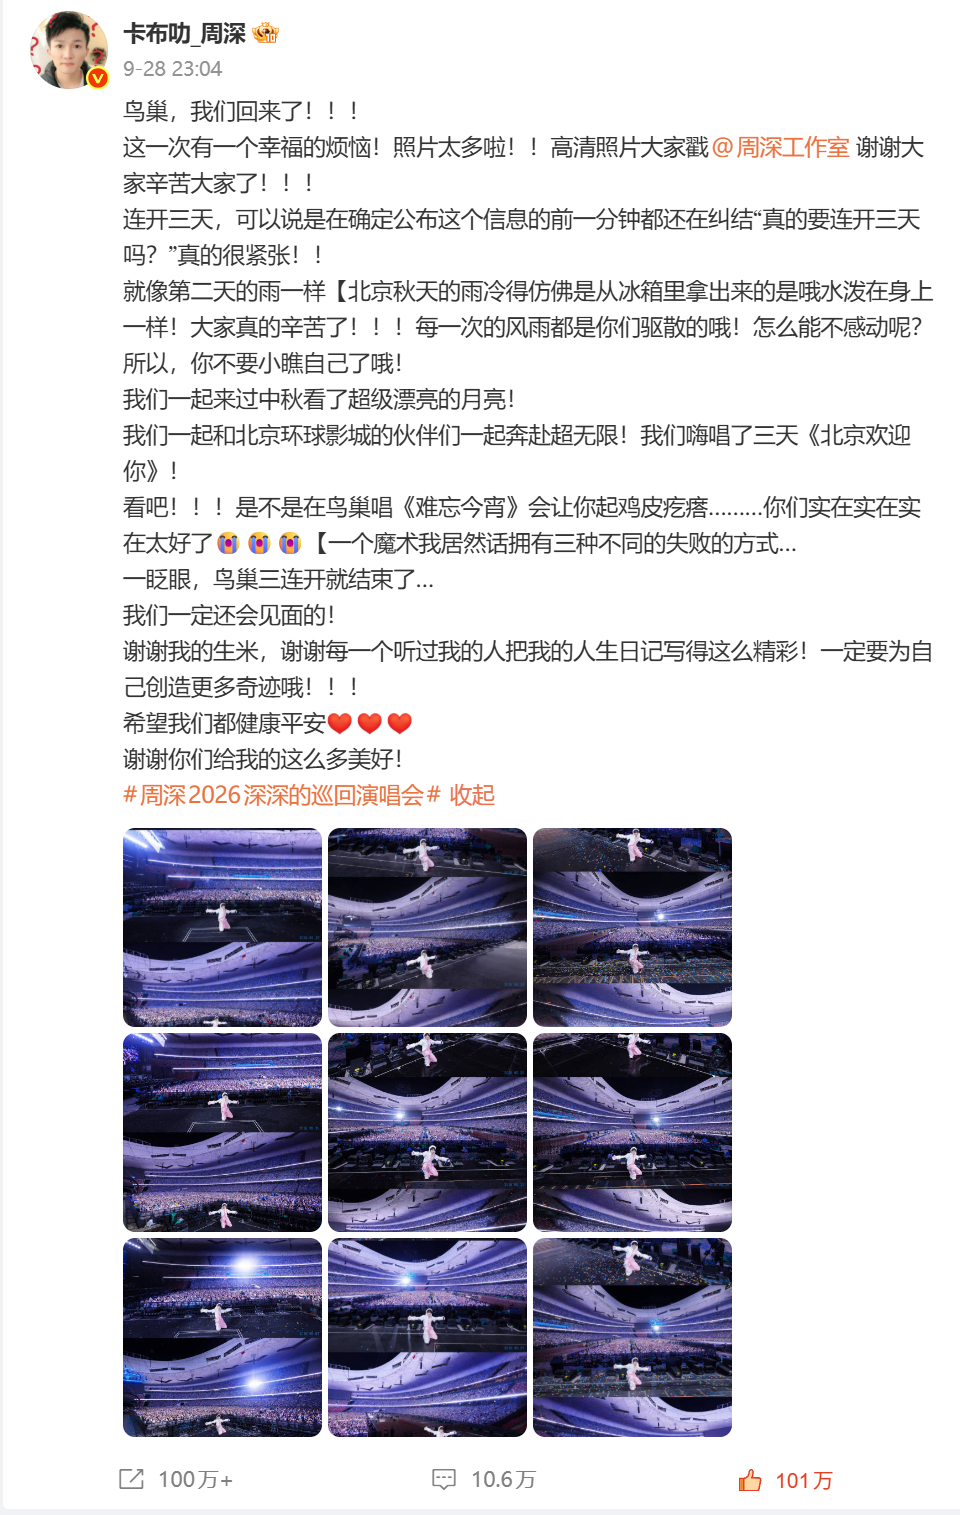
\includegraphics[width=280pt]{img/weibo/BeiJing} 

}

\caption{周深“深深的”巡演2026.09.27北京场告别微博}\label{fig:unnamed-chunk-51}
\end{figure}

\newpage

\section{整理备注（待人工校对，终稿时删除）}\label{ux6574ux7406ux5907ux6ce8ux5f85ux4ebaux5de5ux6821ux5bf9ux7ec8ux7a3fux65f6ux5220ux9664-5}

\begin{enumerate}
\def\labelenumi{\arabic{enumi}.}
\tightlist
\item
  \textbf{录音来源}：023\_2026深深的\_北京0927\_内场1699\_合声版.mp3（约195分53秒，内场1699合声版）。整理方法：按流程 SOP 全场分段多模态转写（40段×5分钟），唱词对照《appendixG-2026歌词.Rmd》校正，口号互动逐轮记录，低置信处标〔听写待核〕。
\item
  \textbf{本场定位}：2026年''深深的''巡演第23场（北京 Day3、城市末场，国家体育场''鸟巢''），巡演首次进京且连续三场（周深口播''第一次连续三天开演唱会''\,``我们居然真的在鸟巢连续开了三场''）；国庆前夕（周深口播''预祝大家国庆节快乐''\,``祝我们伟大的祖国生日快乐''）；周深生日（9.29）前两天，全场多次生日祝福。卷首语取自谢幕口播''谢谢你们陪我从街边的舞台，走到Live house，再走到剧场，走到体育馆，再走到体育场，再来到鸟巢！``。北京场特色：问候段教观众清唱《光亮》''莫听穿林打叶声''段（故宫雪景梗，观众接唱''回首向来萧瑟处，也无风雨也无晴''）；达拉崩吧''公主米娅版恶龙''玩笑；记忆商店前气球互动小剧（``有人在笑我的演技，重新来''）；荒城渡歌中现挂''祝你们生日快乐''；大合照时观众合唱《热烈盛开》完整副歌；尾曲《难忘今宵》全场大合唱（周深口播''我想请你们大声的在鸟巢，在今天跟我一起唱这一首歌''）；谢幕BGM《地球没有你》改编版。
\item
  \textbf{关键时间点（按5分钟分段定位，录音全长约195分53秒）}：开场VCR 00:01；修星星的人 约02:39（观众先声合唱首句；``北京站第三场''约04:22）；Try Everything 约07:16；问候+``连续三天/北京话'够噪的'/光亮教学'' 约10:30--12:00；光亮 约13:25（戏曲段约15:20）；若梦 约18:30；浮光/借过一下 约20:25--26:50（两曲与《若梦》在转写稿中时间戳交错，先后按歌单锚点排序，建议人工复核）；机器人VCR 约27:05；请我不改+警报 约30:15--34:00；来啊（``Don't tell me/Lie lie''教学）约34:25--37:57；荧光棒游戏 约38:15（红色=宝贝、恶龙乘以十、公主米娅版恶龙）；达拉崩吧 约41:25；阿木/全名问答 约45:15；反深代词口播 约46:00；蜃楼VCR（数字倒数）约47:15；天堂岛之歌 约47:40；气球小剧+记忆商店导语 约49:30--51:20；梦见你 约51:30（生日祝福、黑竹荪、气球''扎心''互动约53:30--55:00）；荒城渡 约55:00（``祝你们生日快乐''现挂约56:25）；人是\_ 约57:40；音乐动画VCR 约61:00--64:00；化身孤岛的鲸 约64:05（墙头梗约67:55--68:55）；花开忘忧 约69:45；我和我的祖国 约74:00--78:40（国庆口播约74:15）；灯火里的中国 约79:05--82:55；小美满 约83:30（许愿约87:00--88:20）；总有美好在路上 约89:15；邓丽君组曲导语 约90:25；独上西楼 约90:00--91:10（``宝你个头''应答约90:00）；路边的野花不要采 约91:15；我只在乎你 约92:15--94:55；面具VCR 约95:10（``很好听''插话、结尾口播变体）；和光同尘 约98:30；云裳羽衣曲 约100:00（``9.29赫兹''应答）；怜悯 约101:45--102:30；望 约102:30--103:45；璀璨冒险人 约103:50--106:00（``十二年前的周深也不敢想''约106:00；周深哽咽与变魔术玩笑约107:00）；奇迹时刻 约108:45；魔术（苍狗、硬币、四颗骰子、小抄）约110:45--113:35；好运来 约113:40；接财运 约118:30（``老鼠干''口播约119:30，待核）；吉量 约119:55--123:00（马年祝福、第三场唱得尤其大声）；想见到气血满满的你 约123:00--123:45；Wala li longla 约123:45--126:00（逐词递进含''Wala li long''）；少管我 约126:00--129:40（绕场口播''转了一圈好开心''约129:35）；点歌饼饼 约130:00；胡同少年志 约135:45；点歌阿琳/盼盼 约143:30；嗨 约148:05；梨花颂 约154:45；北京欢迎你 约155:15--160:00；周可可/周嫑嫑 约160:50；致谢 约162:35（云南白药、金少刚Polo衫应答、安栋小西装/军大衣、螺蛳粉口播、微博/微博音乐/微博演出、超话热聊）；大合照 约173:45（抹布造型玩笑约174:40；观众合唱《热烈盛开》约175:40）；我以渺小爱你 约177:20；交换日记VCR 约184:15（周深宝贝齐呼约186:10）；起风了 约186:55（``以爱之名你还愿意吗''约191:10）；大鱼 约192:20；难忘今宵 约194:35--195:00（国庆祝福、告别长口播）；谢幕BGM《地球没有你》 约195:10（录音至195:53结束）〔后段时间点为5分钟分段估算，建议人工复核〕。
\item
  \textbf{点歌观众}：第一位饼饼（安徽人，幼时迁居云南昆明；自述第一场是2026.05.31重庆场；第一首《化身孤岛的鲸》，与周深对唱''你的衣衫破旧''段；带来''反身代词，深专大门儿''口音梗〔听写待核〕；三句感言+全场预祝周深生日快乐；点《胡同少年志》并要求''有Wink和弹舌''〔周深玩笑''我没有一首歌叫有Wink呀''〕；与全国各地及海外生米同来）。第二位阿琳（山东青岛，鲁B；新婚，2026.08.01领证，与盼盼同来，看完本场回家办婚礼；第一首《大鱼》并清唱；点《反深代词》中的《嗨》，祝''深深身体健康，少淋雨，多唱好听的歌''；周深以''所有的幸福都在你转身的时候发现。嗨，他就在你身边哦''作结；两人合照两张）。
\item
  \textbf{VCR 差异}：开场、机器人、面具、交换日记四段 VCR 与《appendixD-2026VCR文字版.Rmd》一致；面具 VCR 开篇日期行本场为''2026年9月27日，北京''，VCR 中''你的声音好像有点不一样哦，我觉得\ldots\ldots{}``处现场观众插话''很好听！``，结尾口播为''你们会跟我一起大声唱歌，你们说，对吗？``；机器人 VCR 日期句同前两场（''2225年5月17日/第200天/73000天''，数字待核）；交换日记 VCR''只要写下去，就会有精彩''（附录D作''新的彩页''）、``你写着你的迷茫''（附录D作''也许你的迷茫''），均待核。蜃楼 VCR（天堂岛之歌前）本场为数字倒数+机械音效（与前两场''叮咚，有人在门口''不同），附录D未收录，建议补录。音乐动画 VCR 纯音乐无词。
\item
  \textbf{北京场结构差异}（与歌单锚点一致）：Part3 城市限定《我和我的祖国》后紧接《灯火里的中国》、无《小城故事》（邓丽君组曲为独上西楼+路边的野花不要采+我只在乎你）；点歌后加唱《梨花颂》《北京欢迎你》；尾曲《难忘今宵》（国庆前夕全场大合唱）；本场为北京城市末场，正文末尾已按体例加入城市告别微博截图 R 块（img/weibo/BeiJing.png，截图素材由人工保存提供）。
\item
  \textbf{团队名单}（与常州终版一致）：制作必应、总导演周佑洋/庄惟惞、音响总监金少刚、音乐总监安栋、乐尔工作室（调音，现场听作''乐耳''）、南京奥斯泰（音响工程）、北京立超舞台集团（硬体）、时代立方、劳伦斯许工作室/Third Studio/Windowsen（服装）、SDT ShowPro（舞蹈）、大麦（票务总代理）、猫眼/票星球（票务代理）。本场新增致谢：独家冠名云南白药（``本站鸟巢站''）、北京市所有职能部门、场地方国家体育场（鸟巢）、社交媒体微博/微博音乐/微博演出及微博超话、北京这座城市；金少刚（08奥运音响师）与安栋（08奥运点火炬音乐创作者）以奥运梗互动；``安栋老师答应下一次穿军大衣''。
\item
  \textbf{听写存疑}：达拉崩吧公主米娅应答听作''要我爱''（按惯例作''救我啊''，待核）；``阿木''环节观众齐答全名听写不清（转写稿中''梅塔特隆·路西法·奥丁''等长串名疑为模型幻觉，已标注待核，未采用）；修星星的人首句''呼啸的光年''\,``上帝的诗由你我完成''等现场唱词与附录G差异大；若梦/浮光/借过一下三段时间戳交错；记忆商店、怜悯唱段听写不清待补录；云裳羽衣曲''9.29赫兹''应答、结尾唱句与附录G差异；璀璨冒险人''要炙热啊''段听写作''有炙热有不枉''；吉量观众合唱段大面积听写误差已按附录G校正（西河/老鼠夹/激亮/千古树/看庙堂/找明堂/云霞等）；想见到气血满满的你''做好积蓄满满的准备''已校；Wala li longla 现场版唱词（蒙娜丽莎/大西瓜/内向瓜/心里有花吗等）与附录G差异大；少管我''霓虹灯初上热闹出窍''等段差异；``老鼠干''口播；大合照''深深的''应听听作''深圳''；难忘今宵''告别今宵，无论天涯与海角''（附录G作''无论新友与故交''）；谢幕BGM改编版唱词低置信；若干口播（``够噪的''``商量沟通''``在压力她''等）。
\item
  \textbf{唱词校正说明}：正文唱词均按《appendixG-2026歌词.Rmd》校正，主要修正同前两场外，另含：光亮''畅音阁里终一叙''；请我不改/警报串烧段按附录G全词；来啊''要爱就爱放纵吧别退缩''；胡同少年志''更成卯时二刻/匆忙是因为我感伤就要道别/一别京城种兰花/万户灯火少离家/背把三弦走天涯/糖葫芦十颗一串儿/家安在四合小院儿/戏班儿/铜锣儿''；嗨''装满汽水的大海/我像在与风相爱/每一粒像素/让我一片片碎开/随着我心跳开怀/云朵做飞船成排/天空结彩/看我随着风而来/终于对自己够坦白''；我和我的祖国、难忘今宵、热烈盛开（观众合唱段）按附录G；望''绕几千日夜也望向归途''；璀璨冒险人''没人未梦就先懂/忍痛缓行不回头/要逆风不退啊/让痛苦住进你眼眸/多少次传唱''；奇迹时刻全段；吉量全段（羲和/望舒/弱水/祝融/云沙/鸾鸟唱/搅银汤/建木树）；我以渺小爱你''相爱支撑，命才成为生/在时光面前皆我们''；地球没有你（谢幕BGM，录音室版对照，改编版另注）。
\item
  \textbf{待补充}：歌单图（img/playlists/BeiJing-20260927.png）、城市告别微博截图（img/weibo/BeiJing.png）及现场图片待插入。北京三场结构差异（灯火里的中国前移、无小城故事、点歌后加唱梨花颂+北京欢迎你）已按歌单锚点落实。
\end{enumerate}

\chapter{2026.10.17长沙场 (WIP)}\label{ChangSha-20261017}

\begin{quote}
``虽然我已经出道第十二年，但这是第一次来到长沙开演唱会。''------周深
\end{quote}

\begin{figure}

{\centering 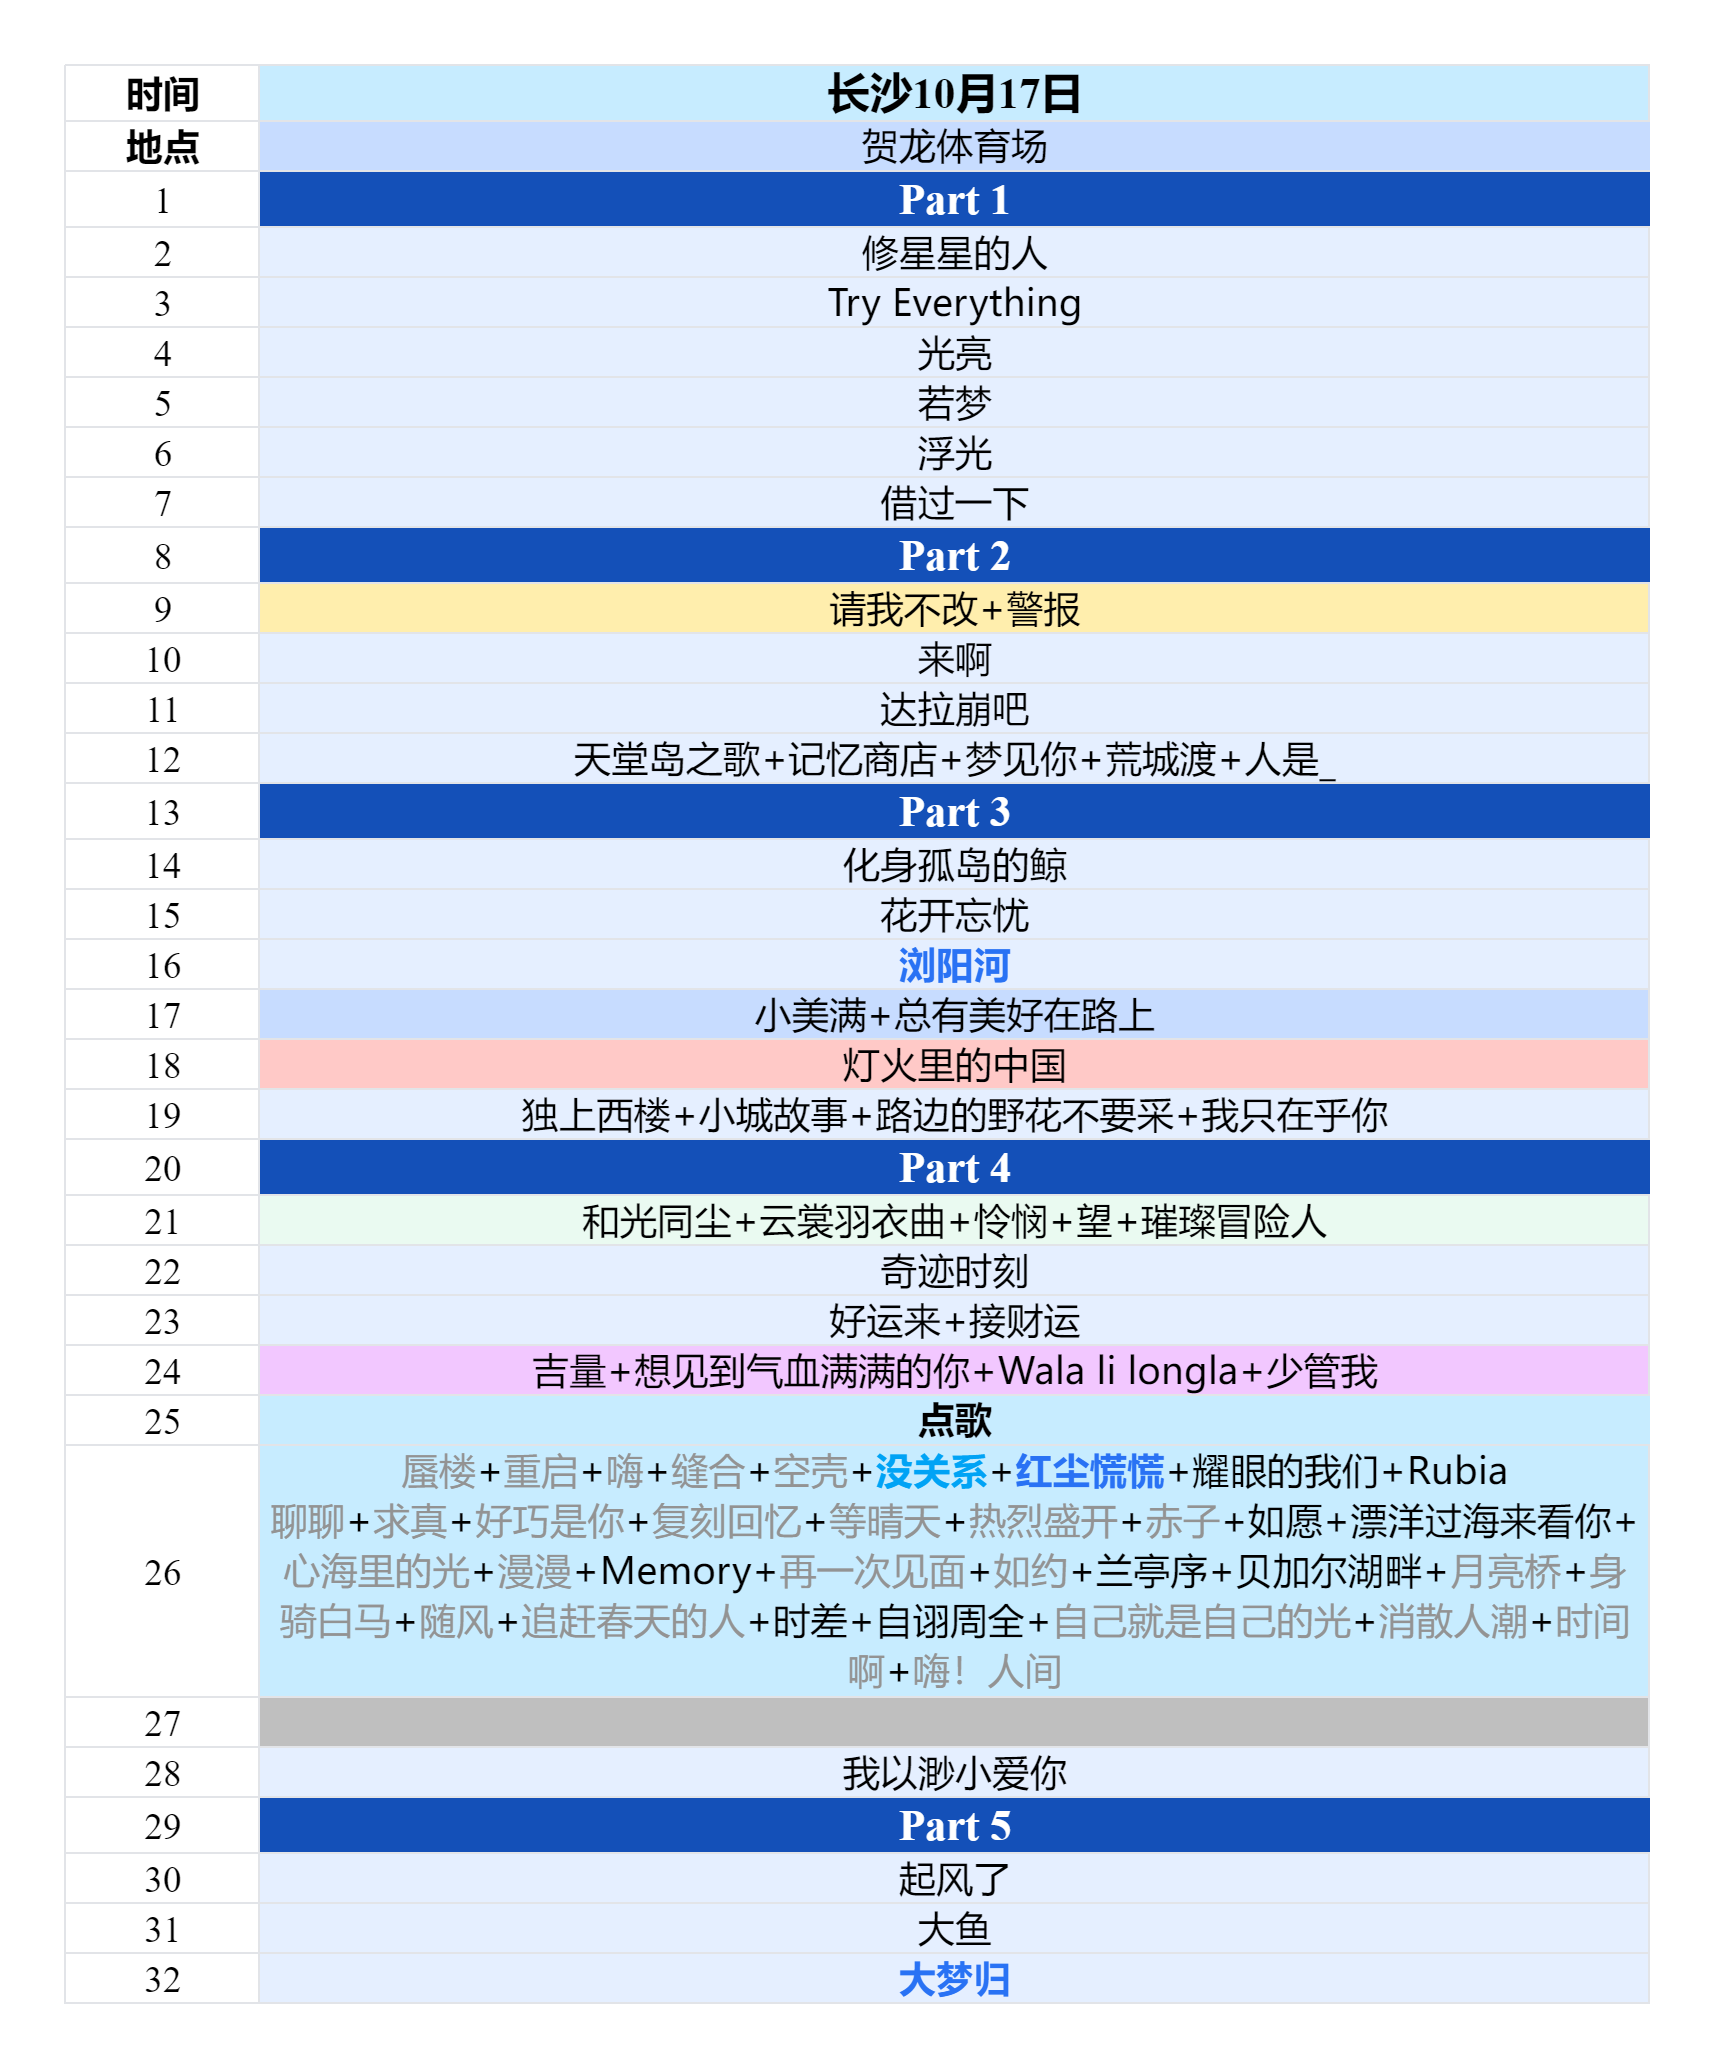
\includegraphics[width=280pt]{img/playlists/ChangSha-20261017} 

}

\caption{2026周深“深深的”巡回演唱会2026.10.17长沙场歌单}\label{fig:unnamed-chunk-53}
\end{figure}

\newpage

\section{Part1}\label{ChangSha-20261017-part1}

\hyperref[opening-vcr]{🎥【\textbf{开场VCR}】}（VCR 正文见附录 D。VCR 结束后《修星星的人》前奏直接响起。）

\hyperref[xiu-xing-xing-de-ren]{🎵【\textbf{修星星的人}】}（米：先声合唱：既然这宇宙让我诞生------）（深：是我在故乡的旷野，仰望银河的夏夜；是我在宇宙的风暴，朝着天仓五飘曳；我的孤独我的热烈，源自137亿年前，几粒星尘的蝴蝶；在噬星的幻灭里，为太阳撑一把雨伞；在时间的深海里，给地球道一声晚安〔首句现场听作''是我在湖上的光影''\,``在失序的光年里''等，已按附录G校正，现场版个别句待核〕）长沙的朋友们你们好吗！（米：好------！）（深：既然这宇宙让我诞生，想必它是要以我为证；我的情感和三十六度的体温，足以暖热即将熄灭的恒星\ldots\ldots 许我以造物的碎屑，重塑文明的边界；许我以渺小的羞怯，挽留物种的毁灭〔第二段主歌现场听作''是我也曾目睹瞬息重塑文明的边界''等，待核〕）（深：既然这宇宙予我重生，想必它是要让我看懂，我的基因和闪闪发光的记忆，足以照亮所有星际的永恒〔现场听作''我的晶莹''\,``星际的流浪''，已按附录G校正〕）（高音吟唱）

\hyperref[try-everything]{🎵【\textbf{Try Everything}】}既然这个宇宙让我们诞生了，那就要勇敢地 Try Everything，好不好？（米：好！）长沙的朋友们，准备好了吗？（米：准备好了！）（深：I messed up tonight, I lost another fight\ldots\ldots No I won't leave, I wanna try everything / I wanna try even though I could fail）（深：Oh oh oh oh oh------）（米：Try everything）（深：Oh oh oh oh oh------）（米：Try everything）（深：Oh oh oh oh oh------）（米：Try everything）（深：Oh oh oh oh oh------）尖叫声！（米：尖叫欢呼声）（深：Look how far you've come, you filled your heart with love\ldots\ldots I'll keep on making those new mistakes / I'll keep on making them every day / Those new mistakes）到你们！（米：Try everything!）再来！（米：Try everything!）再大声！（米：Try everything, oh oh oh oh oh）Try\ldots{}

\hyperref[silver-linings]{🎵【\textbf{光亮}】}长沙的妹陀满哥！〔长沙话''妹子/小伙''称呼〕（米：欢呼声）Try everything. 谢谢你们！（米：欢呼声、尖叫声）哇\ldots\ldots 长沙的朋友们你们好吗？（米：好------！）第一次来到长沙开演唱会。作\ldots\ldots 作为一个湖南人来说，自己也没有想到这么久才来开演唱会的。可能之前想的是因为我们湖南这边来的歌手们实在太多了，不知道大家想不想听歌手周深唱歌嘞？（米：想------！）后面的朋友也想听周深唱歌的不？（米：想------！）谁说这个塑料普通话不是湖南话的一种？我是湖南邵阳的，但是长沙话我真的不太会说。我学了两句，我试一下，大家给我一下鼓励。（米：欢呼声、掌声）长沙的朋友们，大家好，我是周深。谢谢你们来听我的演唱会。长沙的满哥、妹陀都蛮塞嘞！〔长沙话''都很好''之意，听写待核〕（米：欢呼声）要说再多，真的没有学会嘞。但是就想问你们，来听演唱会，你们开心不咯？（米：开心------！）如果大家能玩得开心，那我就是最最最最幸福的人了。因为你们的出现，所以哪怕天色再暗，也永远都是亮着的。因为你们就是光亮。谢谢你们！（米：欢呼声）第一次来长沙开演唱会，才知道这么热的。〔口播听写待核〕你们好吗？（米：好------！）（深：海上一阵风吹起，白云涌向陆地，季风带走沙粒；四季冷暖的交替，多鲜活的生命，有枯萎的痕迹；是奔跑中突然袭来的风雨，是黑暗中一根火柴燃烧的光明；也许你猜不透未知的宿命，像流星飞翔着它却不知目的）可是啊我却------（米：愿意相信）最渺小最微弱最柔软最无畏的你，用尽了全力，努力地回应，再无边再无尽再无解总有一线生机，光亮你自己。我爱你。（米：欢呼声、尖叫声）（戏曲念白＋唱腔两遍：莫听穿林打叶声，一蓑烟雨任平生；畅音阁里终一叙〔听作''畅饮九曲黄河水之水''\,``不管年岁沧海已荒''，已按附录G校正〕，六百年一粟，沧海一梦）谢谢你们的光亮温暖着我。谢谢你们。最无畏的你。（米：欢呼）

\hyperref[like-a-dream]{🎵【\textbf{若梦}】}跟你们的相遇美好的就像一场梦一样。场上的朋友们跟我一起大声唱若梦好不好？（米：好！）（深：浮生若梦，为欢几何；风摇雨落，此心何处停泊；剑起刀割，却斩不断这因果，看天地之间皆漠漠；尘缘萧索，宿命奈何；日升月落，此生依旧难舍；铁马金戈，也踏不碎这心火；忆前尘旧梦，任岁月消磨）全场！（米：往事流转在你眼眸，一边遗忘一边拼凑，如我虔诚合十双手，唯愿你能得到拯救）谢谢你们。（米：我们也爱你！）最大声！（米：往事流转在你眼眸）在哪里？（深唱：一边遗忘一边拼凑）（米：如我虔诚合十双手，唯愿你能得到拯救）长沙的朋友跟我最大声唱！（米：往事流转在你眼眸，一边遗忘一边拼凑，如我虔诚合十双手，唯愿你能得到拯救）〔逐轮记录〕因为\ldots\ldots 你\ldots\ldots 你们\ldots\ldots 就是才得到拯救。〔收束口播听写待核〕

\hyperref[floating-light]{🎵【\textbf{浮光}】}〔本段前另有一段旁白：人生不过三万天，因为遇见了你，才值得留恋。要知道，你的存在非常非常重要，好不好？（米：好！）------与广州场备注''人生恍惚三万天''旁白同源，归属待核〕（深：看指尖拨响蝴蝶，扇动一场离别；我推开无声岁月，续梦一页；你我只是打个照面，可曾有过誓约，走进熟悉却陌生的思念）啊\ldots\ldots（深：你的眼眸装满了时间，你的身后拥故事成篇，此生如梦愿细数流年，与你同写沧海桑田；浮光掠影重山彩云间，你的伏线穿越千百年，人生不过恍惚三万天，漫漫人间，留恋留连〔``你的身后涌动着长篇''``如果来世还能再遇见''等听写已按附录G校正〕）你说那月光照过同样城墙，永恒的刹那此刻沉默无话，想问你这星空是否不曾变化，是啊是啊，我们望着它。〔后段现场唱词听写与附录G差异较大，已按附录G骨架整理〕（米：全场、再大声口令下多轮合唱）〔本段与《若梦》时间戳交错，实际顺序建议人工复核〕

\hyperref[excuse-me]{🎵【\textbf{借过一下}】}（深：少年扬起脸庞，前往他的月亮，人们笑他狂妄，人怎可不一样；白衣过泥潭，怎敢说不染，但凡银两有价，谁能真潇洒；少年爬上城墙，去见他的月亮，破碎几次心脏，得来几句真相；市井或朝堂，四方皆如框，若你生来有刺，磨掉再入场）你们都是对的，他说拜托，让开一下。（深：让我大醉一场，殿堂之上，背闲诗两三章；让我穿白衣裳，过疯人巷，去泥潭捞月光；望大人们见谅，提点的话，我懂也不想装；世人寻黄金乡，我找月亮，何必同往；话谢过，路借过，你是你，我是我）（深：正如先生所说，每颗心都有瑕；潇洒不是不怕，是愿付出代价；权衡利弊后，仍守对与错，谢过赐教的话，路借过一下）你们愿意吗？（米：愿意！）长沙的朋友们你们好吗？（米：好------！）让我听到长沙的朋友们最大声的合唱声。一起！（米合唱：让我大醉一场，殿堂之上，背闲诗两三章；让我穿白衣裳，过风人巷，去你探老月光；望大人们见谅，提点的话，我懂也不想装）再来！（米合唱：人去黄金乡，我找月亮，何必同往。花谢过，路结果，你是你，我是我。〔听写已按附录G校正〕）（米合唱/哼鸣：Wu\ldots{} Wu\ldots）（米合唱：白骨的纠缠，是宿命浪漫〔附录G作''白衣过泥潭，世故里浪漫''等，本段为观众合唱，听写误差大，已按附录G校正骨架〕\ldots\ldots 知心有所爱，不更改；人间多阴霾，若天真犹在，当披上月光，走夜晚）你们，就是我要找的月光。我找到你们了！（米：欢呼声、尖叫声）

\section{Part2}\label{ChangSha-20261017-part2}

\hyperref[robot-vcr]{🎥【\textbf{机器人VCR}】}（VCR 正文见附录 D。VCR 开篇日期句本场听作''2025年5月17日。今天是我被选中执行任务的第200天，系统维持正常运转的73000天''〔数字听写待核〕，其余与附录 D 一致。）

\hyperref[brave-heart]{🎵【\textbf{请我不改}】}长沙！（米：欢呼声、尖叫声）你们在吗？（米：欢呼声、尖叫声）摇起荧光棒！〔VCR 后导语〕（米合唱：是谁在狂？Hey! 还拼命摆？Hey! 说不配我不乖我不失败\ldots\ldots〔现场口号版开场，附录G无对应，听写待核〕）〔与《警报》连唱串烧，独立条目见下〕（深：是谁不断日夜合围向我追来，痛击我最脆弱短板；是谁模糊我的未来，恐惧淹没了期待；绝望已经大军压境，回身却没半个人影，才看清追兵与逃兵，竟都是我自己）请我不改！（米：嘿！）我的姿态！（米：嘿！）我的爱我的痛都与生俱来；请我滚开！〔现场演唱变体，附录G作''请我看开''，待核〕（米：嘿！）我的存在！（米：嘿！）我的明我的暗都不必躲开；我原谅我自己，捡起遗憾拥抱无奈；我允许我放手，让我勇敢活在现在；我不等待！（米：嘿！）我不徘徊！（米：嘿！）我的笑我的泪都不再苍白，放肆盛开。到你们！（米：哈！〔应答听写待核〕）到你们！〔歌中《警报》说唱段听写与附录G差异大（``马拉松尽头是血色惊叹号''等），已按附录G骨架整理，待核〕（深：我发送警报声，血红色惊叹号，提醒你自救；被遥控被耗空，快失控快断送，我替你看透；从借用到利用，到享受到滥用，转身就走，他们绝不为你而痛）〔``我不懂这一生一回抵过一生还能撑多久''等尾段听写与附录G差异大，待核〕请我不改\ldots\ldots 坦荡痛快！（米：嘿！×4轮）〔副歌多轮、合唱逐轮记录〕

\hyperref[jing-bao]{🎵【\textbf{警报}】}〔与《请我不改》连唱串烧〕（深：我发送警报声，血红色惊叹号，提醒你自救；被遥控被耗空，快失控快断送，我替你看透；从借用到利用，到享受到滥用，转身就走，他们绝不为你而痛）〔歌中说唱段''马拉松尽头是血色惊叹号''\,``我不懂这一生一回抵过一生还能撑多久''等听写与附录G差异大，已按附录G骨架整理，待核〕

\hyperref[lai-a]{🎵【\textbf{来啊}】}接下来这首歌，我想让你们帮我一起唱好不好？（米：好！）不会唱的朋友们我教你们一下啊。这首歌叫《来啊》。（米：哦！）就当我唱 Don't tell me（米：来------啊啊啊啊啊）对，就像他们唱的一样，你们要唱''来------啊啊啊啊啊''好不好？（米：好！）试一下啊。Don't tell me（米：来------啊啊啊啊啊）嗯哼，再来一遍哦。Don't tell me（米：来------啊啊啊啊啊）后面的朋友，Don't tell me（米：来------啊啊啊啊啊）等一下就会靠你们咯，求求你们帮帮我好不好？（米：好！）那就，来呀！（观众欢呼声）（深：我，我怎么就这样呆头呆脑，一不小心落入圈套，沉迷的神魂颠倒，Pass off，这灵魂乱七八糟；我，瞳孔里都是你迷人的笑，越靠越近我越浮躁，神涣散虚无缥缈，Cut stop，躁动太纷纷扰扰；天生的怪胎，冲出这阴霾〔现场演唱变体，附录G作''装不出个乖乖''，待核〕；太嘈杂的时代，1v1较量打乱了节拍；别气急败坏，别着急淘汰，一万种防备阻碍，不如就算了，靠过来；将错就错，别拖Let's go，随你操控）全场！Don't tell me lie------我望眼欲穿你别闪躲。Don't tell me lie------那就认怂都别退缩〔现场演唱变体，附录G作''要爱就爱放纵吧别退缩''，待核〕。Don't tell me lie------我倾尽所有赴汤蹈火。Don't tell me lie------如果这就是生活，Let's fall。〔两轮，Why not? 等口令〕我踩到了你的脚。〔对伴舞口播〕谢谢你们！长沙的朋友让我再一次听到你们的尖叫声！太嗨了！后面的朋友你们好吗？

\hyperref[dalabengba]{🎵【\textbf{达拉崩吧}】}好哟，那我们现在又来到了我们深深的巡回演唱会的小游戏环节。这个游戏环节，你可以自行选择你喜欢的颜色，荧光棒可以自己选，选择颜色。分别是四种颜色。我压力已经够大了为什么要吃螺蛳。〔口播玩笑，听写待核〕分别是蓝色、黄色、粉色和绿色。每一个不同的颜色都代表着不同的角色。蓝色代表的是达拉崩吧。黄色代表的是国王陛下。粉色代表的是公主米娅。那绿色代表的是恶龙。这首达拉崩吧应该也是很多朋友们第一次听到歌手周深唱歌对不对？（米：对！）哦，也是在我们湖南卫视参加的节目被大家认知到的对吧？（米：对！）〔``声入人心''湖南卫视梗〕那我们就一起来玩游戏吧。哎呦。我决定，在我们长沙站给大家展示，我到底是否有腹肌。〔玩笑〕看得清吗？看不清是不是？但是你们别忘了我会变魔术哦。给我倒数三个数字。（米：三！二！一！）厉不厉害？（米：厉害！）惊不惊喜？掌声鼓励。那等一下跟我一起来大声的回顾一下这个童话故事好不好？（米：好！）但是别忘了哟，你们不同角色都有相对应的台词，我们试一下啊。当我们喊到\ldots\ldots 达拉崩吧（米：我最棒！）国王陛下（米：再说一次！）公主米娅（米：救我啊！）恶龙（米：嗷呜嗷呜！）〔三轮记录〕有很多长沙的朋友\ldots\ldots 那我们就，我喊长沙你们喊哦该咯。〔长沙话''哦该（搞什么）``，待核〕（米：啊？）好不好？（米：好！）试一下。长沙！（米：哦该！）每到一个城市我还要问这种问题，我真的是哦该咯。为什么嘞？我们试一下好不？求你们咯，好不？（米：好！）因为长沙的朋友们是不是最好啦？（米：是！）怎么说夸你们最好了，下面的朋友说我们不是最好的。〔口播听写待核〕达拉崩吧！（米：我最棒！）国王陛下！（米：再说一次！）公主米娅！（米：救我啊！）恶龙！（米：嗷呜嗷呜！）长沙！（米：哦该！）沙！（米：哦该！）恶龙乘以十，走！（米：嗷呜嗷呜！×10）恶龙来长沙没吃饱。〔玩笑〕恶龙！（米：嗷呜嗷呜！）长沙！（米：哦该！）伤心了。哦该咯你，就是\ldots\ldots 那就一起来唱，达拉崩吧吧！你怕不怕？〔口播〕（深：很久很久以前，巨龙突然出现，带来灾难，带走了公主又消失不见；王国十分危险，世间谁最勇敢，一位勇者赶来大声喊：我要带上最好的剑，翻过最高的山，闯进最深的森林，把公主带回到面前；国王非常高兴，忙问他的姓名，年轻人想了想，他说：陛下我叫，达拉崩吧斑得贝迪卜多比鲁翁；再说一次，达拉崩吧斑得贝迪卜多比鲁翁；是不是，达拉崩吧斑得贝迪卜多比鲁翁；对对，达拉崩吧斑得贝迪卜多比鲁翁）全场！达拉崩吧！（米：我最棒！）国王陛下！（米：再说一次！）公主米娅！（米：救我啊！）恶龙！（米：嗷呜呜！）达拉崩吧！（米：我最棒！）长沙！（米：哦该！）沙！（米：哦该！）达拉崩吧！（米：我最棒！）（深：英雄达拉崩吧，骑上最快的马，带着大家的希望，从城堡里出发；战胜怪兽来袭，获得十二金币，无数伤痕见证，他慢慢升级；偏远美丽村庄，打开所有宝箱，一路风霜伴随，指引前路的圣月光；闯入一座山洞，公主和可怕巨龙，英雄拔出宝剑，巨龙说：我是昆图库塔卡提考特苏瓦西拉松；再来一次，昆图库塔卡提考特苏瓦西拉松；什么是昆特牌提琴烤蛋挞苏打马拉松；不对是昆图库塔卡提考特苏瓦西拉松〔''什么是''已按附录G校正〕）小朋友们！达拉崩吧！（米：我最棒！）国王陛下！（米：再说一次！）公主米娅！（米：救我啊！）恶龙！（米：嗷呜呜！）全场！于是------（深、米：达拉崩吧斑得贝迪卜多比鲁翁，砍向昆图库塔卡提考特苏瓦西拉松；然后昆图库塔卡提考特苏瓦西拉松，咬了达拉崩吧斑得贝迪卜多比鲁翁；最后达拉崩吧斑得贝迪卜多比鲁翁，战胜了昆图库塔卡提考特苏瓦西拉松，救出了公主米娅莫拉苏娜丹妮谢莉红，回到了蒙达鲁克硫斯伯古比奇巴勒城；国王听说达拉崩吧斑得贝迪卜多比鲁翁，打败了昆图库塔卡提考特苏瓦西拉松，就把公主米娅莫拉苏娜丹妮谢莉红，嫁给了达拉崩吧斑得贝迪卜多比鲁翁；啦啦，达拉崩吧公主米娅，幸福得像个童话，他们生下一个孩子，也在天天渐渐长大；为了避免以后麻烦，孩子称作王浩然〔``他的全名十分难念''段录音至此〕）达拉崩吧！（米：我最棒！）国王陛下。（米：再说一次！）公主米娅。（米：救我啊！）恶龙。（米：跑啊！〔应答听写待核，或为''嗷''〕）求你们了。后面的朋友你们会配合我吗？（米：会！）长沙。（米：宝贝！）达拉崩吧的全名是？（米：达拉崩吧斑得贝迪卜多比鲁翁！）十三个字你们都愿意说。欧该咯。三个音节，好不好？长沙。（米：宝贝！）谢谢你们。（演唱）永远依赖你。〔吟唱句听写待核〕尖叫声！我教你们一句长沙话你们都不学吗？欧该咯。（米：宝贝！）这是不是有点过分了我说实话。〔玩笑〕

在前年我发了一张专辑，它叫做\ldots（米：反深代词！）《反深代词》。《反深代词》说的是在两百年后的世界有一个这样一个世界叫做《反深代词》，然后周深一共有十二个不同的情绪碎片，也就是这张专辑当中有十二首不同的歌，如果你在听这张专辑的时候你发现某一首歌跟你的情绪、跟你经历过的故事简直一模一样的，证明我们在两百年后的这个《反深代词》的世界我们彼此相互拥抱了对不对？（米：对！）那在今年，这张专辑终于有实体专辑跟大家见面啦！有没有朋友们跟我一样也已经收到啦？（米：有！）是不是还有朋友们在等？是不是还有朋友们还没有到货？（米：对！）求你们了。长沙。（米：宝贝！）没有一个人配合的。〔玩笑〕好的，那我们来一起看一下在《反深代词》的蜃楼当中，接下来会发生一些什么样的故事呢。

〔蜃楼VCR〕（一个小孩，他生活在梦里。一个故事，还没说出口。一个伤口，正在愈合。〔《天堂岛之歌》前置VCR片段，附录D未收录，建议补录；完整文字待核〕）

\hyperref[haven-song]{🎵【\textbf{天堂岛之歌}】}（深：叮咚，我有一个秘密，悄悄告诉你，欢迎你来到天堂入口。叮咚，有人在按门铃，是谁在外面，把恶作剧当一场游戏。听啊谁在哭泣，看啊谁在窃窃私语，窗外有双眼睛，他在时刻注视着你。叮咚，有人在看你的过去。叮咚，有人在看你的秘密。叮咚，有人在看你的过去。我逃不出去）生米们，你们在哪？（米：在这！〔应答听写待核〕）听过周深唱歌的歌迷朋友们你们在哪？（米：在这！〔应答听写待核〕）（米合唱：有个人从未来，来很古老的年代。醒来的我，很抱歉。〔观众合唱段，或为《记忆商店》``有客人从夜里来，买很古老的年代；亲爱的，我很抱歉''等句，听写待核〕）（米：不说了没有了没有下一站。〔合唱句，或为''不说了没有了没人记得''，听写待核〕×2轮）

\hyperref[the-memory-store]{🎵【\textbf{记忆商店}】}哎？哎？哎这是哪？哦，我是在深深的巡回演唱会对吗？（米：对！）我记得我们有好多好多的暗号，比如像达拉崩吧。（米：我最棒！）唯独有一个暗号绝对不可忘，说对，那就是\ldots\ldots 国王陛下！（米：再说一次！）哦我知道了，就是反身代词〔口播沿误，即《反深代词》〕当中的记忆商店。我们只要拥有这一颗米子心\ldots\ldots（观众笑声）我拿错了，这是我的六块腹肌。〔玩笑〕（观众笑声）只要拥有这一颗米子心，就可以唤醒我们最喜欢、最甜蜜的那段回忆对不对？（米：对！）遇到你们的每一分每一秒，都是我最想要唤醒的记忆。那让我们来看看吧。哎呦哎呦，自己吓到。〔唱段听写不清，唱词见附录G《记忆商店》，待人工补录〕

\hyperref[meng-jian-ni]{🎵【\textbf{梦见你}】}（深：看着眼前还年少的你，恍若流年从未淌过去；时光飞逝就算我也已老去，你却仍有着初见时那双清澈的眼睛；当再一次听你唤出我姓名，我已将一生都历经，明白有些事情早注定；我们都站在时间的河里，离别是相遇的倒影；从初吻后的那天起，就有了再见的含义〔已按附录G校正〕；我望着你远去的背影，渐行渐远直到看不清；时间会改变一切，却再也无法改变你；若多年后还能够有幸，与你重逢在凌晨梦境〔或作''另一场梦境''，待核〕，但愿那时你在人海里，仍将我一眼认清）（米：不说了没有了没有下一站。〔合唱句待核〕×2轮）就这么普通的走过来了？今天没戏啊。哎今天没戏啊。〔对气球互动演员口播〕我有腹肌。（观众：我也有！）你又有个气球。哦，你要同时吹这么多个气球。来给我一个，给我个蓝色的。诶？哇这么多气球唯独没有一个蓝色的。那我们一起来吹，来给我们点鼓励。（观众：欢呼声/掌声、哇！）〔观众席吹气球互动〕时间很紧张哦。来，那让我们来看一下这段回忆是什么样的呢好不好？一起。（观众：欢呼声/掌声）

\hyperref[huang-cheng-du]{🎵【\textbf{荒城渡}】}（深：夜色中寻觅过，当往事困住我，也盼心中生出一点萤火；孤城的传说，有谁来过，将因果赠与我；我在等这因果，渡魂渡魄渡我；纵然已是执着难舍，断了这心魔可原谅我，宿命中获得这解脱，重来过）〔``夜半心中生出''``古城的传说''等听写已按附录G校正〕（深：眼中拂尘，手中残魂，那故事斑驳荒城；修炼天真，拨开心门，握一颗糖暖这孤身颠簸）（米：我说这没有人没人记得〔合唱句，或为''不朽的没有了没人记得''，听写待核〕×2轮）（高音吟唱）

\hyperref[Humans_are_]{🎵【\textbf{人是\_}】}（深：未知摊开棋局，舍弃昨日才可破；再见了我的月光我的蓝我的爱；钢铁的巨兽在轰鸣，我们拒绝走入夜晚；破碎是新生的约定，我便愿为尘埃；让死亡觊觎我，让恐惧亲吻我，来摧毁我深爱的一切，可仍夺不走我的选择；弹指间湮灭我，但命运打不败活着；让生命如剧烈的烟火，璀璨熄灭前也将点亮，孩童的双眸；若巨浪已淹没了来路，我是帆亦是舟；是微渺的希望，我们依然前行，没有放弃〔或作''没有光指引''，已按附录G校正〕，往前吧，失去的，不要停留〔已按附录G校正〕）全场都动起来！（深：让死亡觊觎我\ldots\ldots 孩童的双眸）到你们了！（米：未来的瞳孔〔应答〕）未来的瞳孔。（米：欢呼）以前我也认为那些失去的，没有得到的才是最珍贵的。但是当我遇见了你，听到你唱歌，我才知道我们现在拥有的每一分每一秒才是最宝贵、最值得去好好珍藏的。你们说对吗？（米：对！）（米：有苦痛有欢乐我们记得〔合唱段，附录G无对应，听写待核〕×3轮）是你们创造了不朽的永恒的爱。〔口播〕

\section{Part3}\label{ChangSha-20261017-part3}

\hyperref[music-animations-vcr]{🎥【\textbf{音乐动画VCR}】}（VCR 正文见附录 D，本段为纯音乐动画，无旁白歌词。VCR 前后为纯音乐过场。）

\hyperref[The-whale-who-became-an-island]{🎵【\textbf{化身孤岛的鲸}】}谢谢你们，让我这个化身孤岛的鲸不再孤单。（米：欢呼声）你们找到我了吗？（米：找到了！）（深：我是只化身孤岛的蓝鲸，有着最巨大的身影，鱼虾在身侧穿行，也有飞鸟在背上停；我路过太多太美的奇景，如同伊甸般的仙境，而大海太平太静，多少故事无人倾听；我爱地中海的天晴，爱西伯利亚的雪景，爱万丈高空的鹰，爱肚皮下的藻荇，我在尽心尽力地多情，直到那一天）你的衣衫破旧，而歌声却温柔。（米合唱：陪我漫无目的的四处漂流）（深：我的背脊如荒丘，而你却微笑摆首）（米合唱：把它当成整个宇宙）（深：你与太阳挥手，也同海鸥问候）（米合唱：陪我爱天爱地的四处风流；只是遗憾你终究，无法躺在我胸口，欣赏夜空最辽阔的不朽，把星子放入眸）谢谢你们。（米：欢呼声、掌声）（深：我是只化身孤岛的蓝鲸\ldots\ldots 我有着太冷太清的天性，对天上的她动过情；而云朵太远太轻，辗转之后各安天命；我未入过繁华之境，未听过喧嚣的声音，未见过太多生灵，未有过滚烫心情，所以也未觉大洋正中，有多么安静）当你们\ldots\ldots（米合唱：你的衣衫破旧，而歌声却温柔，陪我漫无目的的四处漂流；我的背脊如荒丘，而你却微笑摆首，把它当成整个宇宙；你与太阳挥手，也同海鸥问候，陪我爱天爱地的四处风流；只是遗憾你终究，无法躺在我胸口，欣赏夜空最辽阔的不朽，把星子放入眸）（深：你的指尖轻柔，抚摸过我所有，风浪冲撞出的丑陋疮口；你眼中有春与秋，胜过我见过爱过的一切山川与河流；曾以为我肩头是那么的宽厚，足够撑起海底那座琼楼，而在你到来之后，它显得如此清瘦，我想给你能奔跑的岸头）（米：没有墙头！〔应答提前，接墙头梗〕）你们到底有多少个\ldots\ldots 墙头？（米：〔听写待核〕（观众喊：大补丸了/太滑了〔旁人喊话，不入正文〕））没有！我稍微解释一下什么叫做墙头呢，就是当我问生米们，你们最喜欢的歌手是谁呀？（米：周深！）他们会说周深，那我就会问他们，你们是不是还喜欢其他的歌手呀？（米：没有！）下面居然有人在回答喜欢。〔玩笑〕没错，我们就是把他们喜欢的其他的歌手，我非常不礼貌地把他们称为''墙头''。所以，长沙的朋友啊，你们到底有多少个墙头嘞？（米：没有！）但是无论怎么样，只要你好好地照顾好自己，好好成为自己，你们都是我的国王和王后。我的国王和王后，谢谢你们来到我的人生日记里。（米：谢谢周深！）长沙的朋友们你们好吗？（米：好！）我们来长沙看你了哟。

\hyperref[Blossoms-that-forget-sorrow]{🎵【\textbf{花开忘忧}】}（深：巷子口买了花，穿过沿街红墙青瓦，夕阳慢慢亲吻着我的白发，推开旧木门回到家；把时光都炖香，而你只是笑不说话；一件遗憾的事，就喝一碗汤，庭院深深，秋叶飘落；我们苍老的时候，就回到小时候，采青梅用来酿酒，你不许偷着喝；穿朴素的衣裳，牵着那衣袖，捡了小猫名为苍狗；我们睡去的时候，像孩子无忧愁，反正也很难上锁，这岁月如小偷；若记忆被偷走了，忘了我的爱，我会说\ldots\ldots）说什么？（米：你好啊！〔听写待核〕）（深：这是给你的花，花的名字叫忘忧草，他说时光汹涌，如水上烟波，别走远了，一起回家）我们一起回家好不好？（米：好！）谢谢你们，能够来到我的地方。谢谢你们！（米：谢谢周深！）（高音吟唱）（深、米：我们苍老的时候，就回到小时候\ldots\ldots 我会说你好啊；在梦里做个梦，看见你我都老了，那永恒没骗我，离散也没有，这份爱只是活在另外时空；如果每一声再见，会开启一个新的空间，每做一个梦，是时空偶尔的重叠；你好吗，离开的人啊，请帮我相爱到剧终）〔合唱逐轮记录〕（深：忘忧草，开着花，你在月光下不说话，一件遗憾的事，就喝一杯茶，庭院深深，秋叶飘落）在我们人生当中，一定有那么一个非常非常珍贵、非常非常重要的人，也藏着那么一份遗憾，再也没有办法见到他。但是我相信，只要我们的思念越大声，他就一定听得到。你们说，对吗？（米：对！）所以一定要好好的照顾好自己，因为他也一定看得到。你们说，对吗？（米：对！）花开忘忧------（米：愿你无忧！）花开忘忧------（米：愿你无忧！）谢谢你们。（米：谢谢周深！）哇，长沙，我们真的来开演唱会啦！（米：哇！）来到长沙站，不知道为什么特别特别的紧张。可能是因为自己\ldots\ldots 嗯\ldots\ldots 在出道之前，一直都在听说长沙这个城市，但是从来都没有来过。因为我一直也都像，在刚才那个动画片里面，大家记得有一个从山里面出发的孩子吗？（米：记得！）那个就是我。所以非常开心，谢谢每一位最善良、最美好的你，把我带到了长沙，带到了一个又一个城市的体育场开演唱会。谢谢你们为我创造的奇迹！（米：谢谢周深！）关于我们湖南的歌曲有很多首，那这首你们会唱吗？（米：会！）（深清唱：这里的山路十八弯，这里的水路九连环\ldots\ldots〔《山路十八弯》〕）会唱的朋友比较少数。那这首歌会唱吗？（深清唱：浏阳河，弯过了几道弯，几十里水路到湘江。）（米：浏阳河，弯过了几道弯，几十里水路到湘江。）同样都是歌曲，区别这么大。〔玩笑〕那等一下让我听到你们最大的合唱声好不好？（米：好！）谢谢你们。

\hyperref[liu-yang-he]{🎵【\textbf{浏阳河}】}你们知道答案吗？（米：知道！）我也知道啊。你们看我唱得对不对啊？（深、米：浏阳河，弯过了九道弯，五十里水路到湘江。江边有个湘潭县哪，出了个毛主席，领导人民得解放，啊依呀依子哟。）等一下让我听到你们最大的声音好不好？（米：好------！）后面的朋友们准备好了吗？三、二、一，唱！（全场大合唱：浏阳河，弯过了九道弯，五十里水路到湘江。江边有个湘潭县哪，出了个毛主席，领导人民得解放，啊依呀依子哟。）〔两轮大合唱＋``出了个毛主席，领导人民得解放''单句一轮，逐轮记录〕那这首，你们会唱不咯？（米：会------！）会唱吗？（米：会------！）让我听到你们的声音好不好？

\hyperref[simple-bliss]{🎵【\textbf{小美满}】}（深、米：没什么大愿望，没有什么事要赶；看见路口红灯一直闪，它像眨眼的小太阳；乌云还挺大胆，顶在头上吹不散，我抓在手里捏成棉花糖，什么烦恼不能忘；既然是路一定有转弯，哪个风景都漂亮，揉揉疲惫的眼睛停下来看一看，美好简单）全场一起！（全场大合唱：你看小狗在叫，树叶会笑，风声在呢喃；不如好好欣赏一秒，迷迷糊糊的浪漫；只要一觉醒来，床单洒满阳光的温暖；不去想，不必想，不用急急忙忙说一个答案）谢谢你们。（米：谢谢周深！）不是谢谢你们，不是谢谢周深哟。〔口播听写待核〕（米：谢谢周深！）（合唱：笑一笑就灿烂）长沙的朋友们你们好吗？（米：好！）

（许愿环节）让我们一起在《小美满》这首歌当中许愿吧，好不好？（米：好！）要相信，相信的力量，相信美好的力量。我们一起，像我这样，我给你举个例子哦。我们闭上眼睛，想好你的愿望。然后我会倒数三个数字，三、二、一，叫你睁开眼睛，我们的愿望就会出现在这棵许愿树上。现场的每一位朋友，无论什么年龄段，无论什么职业，请相信美好的力量，我们一起许愿吧。闭上眼睛。想一想，你生日的时候第一个蹦出来的愿望是什么呢？想一想，你一直以来都想要实现的愿望是哪一个呢？哦对了，《小美满》这首歌当中的愿望有一个要求，只能够许关于自己的愿望。想一想，是不是很久没有拥抱一下自己？是不是没有跟自己说一声，你辛苦啦，你走到今天真的真的很厉害呀。三、二、一，睁开眼睛！（合唱：你愿相信什么就把世界看成什么样，偶尔难题加点重量也要轻轻地旋转，所以无论如何记得保管小小的光环；笑就好哭也好，今天就是明天最好的陪伴；笑也好，哭也好）到你们！（合唱：自己是自己最好的陪伴）你们都是周深最好的陪伴。谢谢你们！（米：谢谢周深！）因为你们的出现，每一天都变得非常非常的特别。让我们祝今天过生日的朋友------（米：生日快乐！）让我们祝昨天或者是前一段时间过生日的朋友------（米：生日快乐！）也让我们祝明天或者过一段时间过生日的朋友------（米：生日快乐！）因为你的诞生，每一天都值得珍惜哦。也因为遇见了你，我才看见。

\hyperref[zong-you-mei-hao-zai-lu-shang]{🎵【\textbf{总有美好在路上}】}（合唱：花在开云在飘笑容在脸上，我们向前方一路向阳）亲爱的你！（合唱：亲爱的你在路上慢慢逛看一看太阳，让风轻轻吹拂你的脸庞，今天过去要到明天看看天气会怎样；抬头发现，你们就是光芒〔``雨过晴朗故事都慢慢香（长）''等听写与附录G差异大，已按附录G校正，末句现场合唱或作''你们就是光芒''，待核〕）（米：呜------！）

\hyperref[deng-huo-li-de-zhong-guo]{🎵【\textbf{灯火里的中国}】}灯火里的中国，美不美丽？（米：美丽！）那是因为由每一个最美好的你组成的哟。好好照顾好自己好不好？（米：好！）（深、米：都市的街巷已灯影婆娑，社区暖暖流淌的欢乐；远山的村落火苗闪烁，渐渐明亮小康的思索；归港的船帆从灯塔掠过，追梦脚步月下交错；广场焰火在节日诉说，星空升腾时代的巍峨；灯火里的中国青春婀娜，灯火里的中国胸怀辽阔，灯火漫卷的万里山河，初心换回了百年承诺；灯火灿烂的中国梦，灯火荡漾着心中的歌）等下跟我一起大声唱好不好？（米：好！）好不好？（米：好！）（深：归港的船帆从灯塔掠过，追梦脚步月下交错，广场焰火在节日诉说，星空升腾时代的巍峨）全场！（米合唱：灯火里的中国青春婀娜）再大声！（米合唱：灯火里的中国胸怀辽阔）（米合唱：灯火漫卷的万里山河，初心换回了百年承诺；灯火里的中国青春婀娜，灯火里的中国胸怀辽阔，灯火灿烂的中国梦，灯火荡漾着心中的歌）〔多轮逐轮记录〕哎我刚才没有听到这边的朋友唱。大家再给我唱一遍好不好？（米：好！）清一下嗓子哈。（米合唱：灯火里的中国）（深：青春婀娜！）（米合唱：青春婀娜）后面呢？（米合唱：灯火里的中国胸怀辽阔，灯火漫卷的万里山河，初心换回了百年承诺）再来一遍！（米合唱：灯火里的中国青春婀娜\ldots\ldots 灯火荡漾着心中的歌）哇，还有和声！为自己鼓掌！

🎵【\textbf{邓丽君组曲}】谢谢大家。我呢，希望自己可以成为自己的、像偶像那样的歌手的存在的歌手。〔口播听写待核〕我有一位非常非常喜欢的歌手，叫做邓丽君女士。你们会唱她的歌吗？（米：会！）我也希望能够像她一样，有好多好多首歌去存放着你们的记忆，就像一颗颗时间胶囊一样。那如果等一下有你会唱的歌，你就跟我一起唱好不好？（米：好！）

\hyperref[du-shang-xi-lou]{🎵【\textbf{独上西楼}】}（深：无言独上西楼，月如钩。寂寞梧桐，深院锁清秋。剪不断，理还乱，是离愁）（米：没有墙头！）（深：是离愁。）（米：没有！）（深：别是一般滋味在心头。）（米：没有！）（深：是不是你们的墙头？）（米：没有！不是！）不是\ldots\ldots〔玩笑〕

\hyperref[xiao-cheng-gu-shi]{🎵【\textbf{小城故事}】}（深：小城故事多，充满喜和乐。若是你到小城来，收获特别多。）我们现在在的城市是？（米：长沙！）（深唱：唱山歌嘞，这边唱来那边和。〔《刘三姐》现挂〕）（米：唱山歌，这边唱来那边和。）（深：若是你到长沙来，收获特别多。〔现场改词〕）都有些什么呀？（米：看似一幅画。）还有呢？（米：听像一首歌。）后面的朋友大声唱！（米：人生境界真善美，这里已包括。）（深：谈的谈，说的说，长沙的朋友谁的墙头多？〔现场改词〕）（米：没有！）（深：请你的朋友一起来，来哪里？）（米：长沙来做客。）来，你们大声邀请！（深：请你的朋友一起来，来哪里？）（米：长沙来做客。）

\hyperref[donot-pick-the-roadside-flowers]{🎵【\textbf{路边的野花不要采}】}这首歌会唱吗？（米：会！）一起唱！（深、米：送你送到小村外，有句话儿要交代。虽然已经是百花开，路边的野花你不要采。）那是怎么了？你们唱！（米：路边的野花你不要采！）最大声！（米：你不要采！）一起唱！（深、米：记着我的情，记着我的爱，记着有我天天在等待。我在等着你回来。千万不要把我来忘怀，千万不要把我来忘怀，千万不要把我来忘怀）

\hyperref[I-only-care-about-you]{🎵【\textbf{我只在乎你}】}（米：哇------！）我想过很多次，也没有想出来，如果没有被你听见、被你看见，我现在在干什么呢？（深、米：如果没有遇见你，我将会是在哪里？日子过得怎么样？人生是否要珍惜？也许认识某一人，过着平凡的日子，不知道会不会，也有爱情甜如蜜；任时光匆匆流去，我只在乎你，心甘情愿感染你的气息）唱！（米：人生几何能够得到知己，失去生命的力量也不可惜）大声唱！（深、米：所以我求求你，别让我离开你，除了你我不能感到一丝丝情意）全场最大声！（深、米：任时光匆匆流去，我只在乎你，心甘情愿感染你的气息；人生几何能够得到知己，失去生命的力量也不可惜；所以我求求你，别让我离开你，除了你我不能感到一丝丝情意）你们\ldots\ldots（米：除了你我不能感到一丝丝情意）你们会忘了我吗？（米：不会！！！）（深、米：除了你我不能感到一丝丝情意）

\section{Part4}\label{ChangSha-20261017-part4}

\hyperref[mask-vcr]{🎥【\textbf{面具VCR}】}（VCR 正文见附录 D。开篇日期行本场为''2026年，10月17日，长沙''，其余与附录 D 一致。）

（米：对！）〔回应 VCR 结尾''你说，对吗？``〕没听到哦。（米：对！）你说，对吗？（米：对！）你们会跟我一起唱歌，你们说，对吗？（米：对！）你们好。

\hyperref[stay-with-light]{🎵【\textbf{和光同尘}】}（深、米：和你一起歌唱，和你一起唱〔附录G作''和你一起歌，和你一起合''，现场合唱记法，待核〕。月落星辰〔附录G作''月落星沉''，待核〕，日出东方）（深、米：和你走过万水千山。〔附录G作''和你走过理想的大河''，现场合唱听写差异大，待核〕）（深：从容着，沸腾着。）（深、米：你看那盛放的花，来自期盼的种子。你看那丰硕果实，来自耕耘的浪漫。宽广的大河，来自八方汇聚的小溪。奔腾向前的大江，来自高山的哺育。和光同行，跌跌撞撞。和光同路〔附录G作''和光同舞''，现场演唱变体，待核〕，翻过山岗〔附录G作''奋不顾身的坎坷''，待核〕。和光同尘，不为盛名而来〔现场听作''不为生命而来''，已按附录G校正〕，不为低谷而去。和光同尘，为你而来，有你我在。）

\hyperref[Song-of-the-cloud-dress]{🎵【\textbf{云裳羽衣曲}】}我们的缘分一定不会太浅，因为我的名字叫\ldots\ldots（米：周深！）因为我们巡回演唱会的名字叫\ldots\ldots（米：深深感谢你！〔应答听写待核，或为''深深的''〕）（深：故事鲜艳，而缘分却太浅。）（米：我的爱恋竟如此的明显。）（深：我不停的默念，想牢记你的容颜。你们来。）（深、米：故事鲜艳，而结局却搁浅。这些年，你又在那座红尘之间，幻化成哪张脸？）（深：云起不知何时，雪落不知时节。长夜与你诀别，何日能再见？漫天飞舞的黄沙，迷了眼。曾经的光阴，在心里。〔本段为观众合唱/现场变体，与附录G''你轻落指尖，月下拨弄琴弦，一曲云裳羽衣恋，人世间，漫天飞舞着思念''差异大，待核〕）

\hyperref[lian-min]{🎵【\textbf{怜悯}】}（深：我要比你显得更无情。）（米：看这天地苍地，任你去讨来的公平。〔现场应和句，附录G无对应，听写待核〕）（深：我要带着爱恨着你。）（米：旁人就没法你再欺。〔现场应和句，听写待核〕）（深：我要唱着歌顶天立地，站成中心。）（深、米：告诉人间天地，生的意义，千里共婵娟。〔现场应和句，听写待核〕）〔唱段听写不清，唱词见附录G《怜悯》，待人工补录〕我们不要祈求怜悯。我们都值得被好好爱着，对不对？（米：对！）无论在哪儿，都会绕回彼此身边，对不对？（米：对！）

\hyperref[Expectation]{🎵【\textbf{望}】}（深、米：我们总会绕啊绕，绕啊绕，绕几千里路也望向归途。乘着风，想念吹拂。手中线绕啊绕，绕啊绕，绕几千日夜也望向归途。燕归巢迁徙之路，参与者无数，待到烟火照夜白时准备庆祝。我们心有所住〔``往向归宿''听写已按附录G校正〕。）（深、米：我们总会绕啊绕，绕啊绕，绕几千里路也望向归途。乘着风思念吹拂，游夜空漂浮，抓一颗流星做礼物，愿你幸福；手中线绕啊绕，绕啊绕，绕几千日夜也望向归途；燕归巢迁徙之路，参与者无数，待到烟火照夜白时准备庆祝，我们心有所住）〔多轮逐轮记录〕

\hyperref[adventurers]{🎵【\textbf{璀璨冒险人}】}璀璨冒险人们，你们准备好了吗？（米：准备好了！）让我听到你的声音！（深、米：他们说要越过前方风沙必须低着头，他们说要绕过蜿蜒的河才能往前走；他们说烫要放手，太远要换个路口，如果得不到谁的认同，那就不算拥有；没人能够决定谁的一生应该怎么活，没人能够定义谁的天空是什么颜色；没人未梦就先懂，只是单纯相信着，背向光的英雄，每张轮廓出自平凡的沉默）你们的存在，就是我的英雄！（米：欢呼）（深、米：沿途一身泥泞跌撞的是我，忍痛缓行不回头的也是我；就让一路曲折每一道伤口，洗净我的脆弱）全场最大声！（深、米：原来咽回去的泪，才能淹没了脆弱，我发誓更勇敢一生与梦相拥；还想要继续吗？有逆风不退啊，让痛苦住进你眼眸；别怕未来的模样，辜负曾经的凝望，有多少理想就有多少次传唱〔``穿肠''听写已按附录G校正〕；那沿途的风浪，也不过就这样，这一路光景有你在身旁；有炙热的光，有滚烫的光，有勇往的光〔``要炙热啊，要不枉啊，要勇往啊''听写已按附录G校正〕；起风了，呼唤了，你还在等什么；挥手了，再见了，别不舍回头啊，像心中的梦啊，去追吧〔``向''听写已按附录G校正〕）（深：要多渺小的人才算孤独〔附录G作''要能留下伤痕才算活过''，现场唱词待核〕；要你记得，要你懂得〔附录G作''愿你记得，愿你哭过''，待核〕，不惧脆弱。不惧脆弱。不惧脆弱。〔现场重复〕）希望你永远无畏，永远有勇气，也同样不要害怕看到自己脆弱的一面，好吗？（米：好！）因为它也是组成最完美的我们的一部分。希望你勇敢向前冲，也不惧脆弱。（米：欢呼声）是\ldots\ldots 是你们的出现\ldots\ldots（米：尖叫声）大家也会觉得很奇怪，为什么你们此处要尖叫。〔口播，接变魔术自嘲〕（米：尖叫声、笑声）是你们的出现，让曾经那个不敢唱歌的周深，变成歌手去到一个又一个的体育场开演唱会。也是你们的出现，让周深一次又一次地变魔术。（米：大笑声、欢呼声）

\hyperref[miracle-moment]{🎵【\textbf{奇迹时刻}】}被你们看到的每一秒，都叫做奇迹时刻。（深：从银河抹去的恒星，穿梭时空的王牌，一个瞬息就能将不思议解开〔现场听作''借一抹抹去的晨曦，当作时空的门牌''等，已按附录G校正〕；礼帽会翻出精灵，还是一整片星海，那悬念在左手或右手，never know；这世界总有太多陆离光怪，以惊喜回应期待，We can dream, we can fly；若相信谁都可以重塑现在，不需要等待，Show time，此刻就无限精彩；I wanna see my way in starlight，奇迹时刻等你一起来；We gonna change the fate never deny，以无数颗渺小的光彩，就能照亮无穷未来）〔``就算生活充满竞赛''等现场增唱段，附录G无对应，待核〕场上的朋友们你们好吗？（米：好！）我要开始变魔术了你们怕不怕？（米：不怕！）不怕。我跟你们说我今天的魔术很厉害，我是不怕特写的。特写机位过来。掌声在哪里？（米：欢呼声）【魔术环节】大家有看到这是一个非常普通的三个隔开的格子对不对？（米：对！）这是个非常可爱的蓝色小狗狗对不对？（米：对！）没有问题吗？现在我们把它放在中间，来跟我\ldots\ldots 什么都问没有问题啊。〔口播听写待核〕帮我倒数三个数字，来三、二、一！（米：三！二！一！）噔噔！（米：哇！）这边是两个了对不对？（米：对！）看哦，两边一样，一边放一个。再来三二一，三、二、一！（米：惊呼/欢呼声）哈哈哈哈哈。咱们喊一遍三二一，三、二、一！（米：三！二！一！）（笑声）这个魔术呢，哈哈，这个很厉害。我可以随机抽出我们等下随便选出来的一个数字你们信不信？（米：信！）我随便洗你们喊停啊，然后我们就第一张牌啊，来。比较随机性的话我们随便抓一张哦。（米：欢呼声）这是什么？方片六。大家看这是一个非常普通的牌，对不对？（米：对！）来喽。你们继续看着啊。刚才那张牌是什么？（米：方片六！）你看大家看，这是随便都是\ldots\ldots 不要吵着我变魔术啊，很容易失败的。〔玩笑〕所有的牌都没问题吧？都是正向的朝着一个方向对不对？（米：对！）对不对？大家看一下。哎！啊，方片六对不对？（米：对！）那如果\ldots\ldots 突然你看啊，大家看着看着。看着看着，这里是不是有一张是反过来的？（米：啊！）那它会是\ldots\ldots（米：哇！）（米：哦，骄傲的嘞！啊，多骄傲。〔观众议论，不入正文，备注存档〕）大家可能会觉得是不是所有的刚才反的那一面那个是不是方片六？我给你们看哦，这张，它是不是？（米：不是！）所以，掌声在哪里呀？（米：哇！）周深厉不厉害？（米：厉害！）变魔术厉不厉害？（米：厉害！）那好运来了你们接不接？（米：接！）没有想到有一天变魔术成功了，会看到你们失望的表情。〔玩笑〕

\hyperref[good-fortune-comes]{🎵【\textbf{好运来}】}（深、米：好运来祝你好运来，好运带来了喜和爱，好运来我们好运来，迎着好运兴旺发达通四海）（深：叠个千纸鹤再系个红飘带，愿善良的人们天天好运来；你勤劳生活美，你健康春常在，你一生的忙碌为了笑逐颜开；打个中国结，请春风剪个彩，愿祖国的日月年年好运来；你凤舞太平年，你龙腾新时代，你幸福的家园迎来百花盛开）大声唱！（深、米：好运来祝你好运来\ldots\ldots 通四海）身体健康，接不接？（米：接！）恭喜发财，接不接？（米：接！）（深：叠个千纸鹤\ldots\ldots 迎来百花盛开）最大声！再大声！（深、米：好运来祝你好运来\ldots\ldots 通四海）〔两轮〕长沙的朋友们你们好不好？（米：好！）后面的朋友你们好不好？（米：好！）所有朋友我们用最大的声音接最美的祝福好不好？（米：好！）跟我一起，接平安！（米：接平安！）接幸福！（米：接幸福！）接健康！（米：接健康！）接财运！（米：接财运！）

\hyperref[jie-cai-yun]{🎵【\textbf{接财运}】}（深、米：接个好运来接个好起来，接财神开开心心到家里来〔附录G作''接个财神开开心心到我家里来''，现场合唱记法，待核〕；接个财运来小财大财，都接都接都接进山与海〔附录G作''我接我接，我接金山银海''，现场合唱记法，待核〕；好运来我接个好运来\ldots\ldots 嘿！接个运到来〔或作''我接满亿口袋''，听写待核〕）祝长沙的朋友！（米：恭喜发财！）恭喜发财，接不接？（米：接！）这三只青蛙你们等一会儿。四只，居然有四只这样奇怪的青蛙。葫芦娃的即视感。〔口播玩笑，听写待核〕数还是太少了。要不然他们也应该很难出现在这里。〔口播听写待核〕但无论怎么样都是想要祝福每一个人身体都顶呱呱，你们接不接？（米：接！）那我希望坐着我们的小车车来看一下有谁没有好好的接好运哦。祝大家在马年拥有无量的吉祥，你们准备好了吗？（米：准备好了！）我们来咯。

\hyperref[ji-liang]{🎵【\textbf{吉量}】}（米：谁在车上系铃铛〔``羲和车上金铃铛''听写，已按附录G校正〕，叮当叮当，叮当叮当。魔术家后一尾巴〔``望舒驾后银尾巴''听写，已按附录G校正〕，摇摇晃晃，摇摇晃晃。河水岸边换吉量〔``弱水岸边唤吉量''听写，已按附录G校正〕，吉量吉量，叮叮当当，叮叮叮叮当当。）（深：九天之上飘来一朵雪花，原来是我那英俊的小马；金色星星在它眼里安家，祝融手持火种编织了它的发〔``初生树枝不多''听写已按附录G校正〕）你们好吗？（米：好！）（深：我的小马一天一天长大，穿过凛冬和最沸腾的夏，驮来西边石头东边的花〔``衔来''听写已按附录G校正〕，马蹄扬起层层层层的冰沙〔``云沙''听写已按附录G校正〕）会唱的跟我一起。（米：翻过山川和鸟唱〔``高高山上鸾鸟唱''听写，已按附录G校正〕，叮当叮当。过海浪里找樱桃〔``东海浪里搅银汤''听写，已按附录G校正〕，叮叮当当。千棵树下换吉量〔``建木树下唤吉量''听写，已按附录G校正〕，吉量吉量，叮叮当当，叮叮叮叮当当。）长沙的朋友们好吗？（米：吉量，我勇敢的小马，当人间需要桥梁，请你垂下缰；吉量，树顶上那颗太阳，在山谷里绽放〔附录G作''在晨雾里张望''〕，风带来梦盛放〔附录G作''驮它来我身旁''〕〔本段合唱听写与附录G差异大，待核〕）你们好吗？（米：谁在车上系铃铛，叮当叮当\ldots\ldots〔重复合唱〕）尖叫声！你们好吗？（米：好！）请问你是谁？你是自己的？（米：宝贝！）宝贝？（米：啊！）

\hyperref[xiang-jian-dao-qi-xue-man-man-de-ni]{🎵【\textbf{想见到气血满满的你}】}（深：感觉自己多珍贵，还会有更好的等着你，还有好多梦在飞，还要给自己一个新的机会。你要早些早睡，别那么累，做好情绪慢慢的准备〔附录G作''要早起早睡''\,``气血满满''〕〔现场唱词与附录G差异处已照词校正，``情绪''待核〕；想见到你，灿烂的你，不惧也无畏〔附录G作''无惧也无畏''〕；别害怕疼痛，别怕眼泪，就让我来陪着你找回，手里有暖，心里有暖，远方的明媚〔附录G作''阳光的明媚''，待核〕）你们好吗？（米：好！）（深：就让存在的在它的时候〔与附录G''有再疼再冷再怕的时候''对应段听写差异大，待核〕（米：清晰记得〔应和句待核〕）（米：我永远会是你依靠的身侧〔附录G作''我永远会是你停靠的选择''，听写已校正〕）唯有梦可贵，勇气可贵，藏起热情慢慢的加倍〔附录G作''举起热情满满的奖杯''，听写待核〕；那时的你，灿烂的你，不惧也无畏；无论多少岁，此生来陪〔附录G作''精神百倍''〕；我都会来陪着你找回，手里有暖，心里有暖，远方的明媚）长沙的朋友们你们好不咯？（米：好！）请问你是谁？你是自己的？（米：宝贝！）宝贝！

\hyperref[wala-li-longla]{🎵【\textbf{Wala li longla}】}前年发的专辑，里面有个快乐密码。等一下跟我一起大声喊这个快乐密码好不好？（米：好！）我教一下你们哟。哇啦哩隆啦！（米：哇啦哩隆啦！）长沙的朋友们嘞，哇啦哩隆啦！（米：哇啦哩隆啦！）全场最大声，哇啦哩隆啦！（米：哇啦哩隆啦！）（深：把蜗牛都放大，把气泡堆成塔，口味自由混搭，用沙粒提炼火花；无所谓章法，无所谓多伟大，一默念就触发）尖叫声！（米：啊------！）（深、米：哇啦哩隆啦；充电咒语是一串长代码〔现场版唱词，附录G无对应，待核〕；心里有花啦；幸运会解码成烟花喷洒〔附录G作''心愿会解码成烟花挥洒''〕；别爱讲反话，怕尴尬理他〔现场版唱词，待核〕；甜美唤醒它；烦恼没时差；哇啦哩隆啦）你们好吗？（深、米：我看那浪花不只是浪花；也不过云是风的骨架〔现场版唱词，待核〕；快乐没时差。哈喽？哇啦哩隆啦；我看到永恒都像一刹那；虚拟与现实也能融洽〔附录G作''无缝融洽''〕；哇啦哩隆啦）你们好吗？（深、米：快乐最伟大）谢谢你们来跟我们见面！（间奏欢呼）场上的朋友们你们准备好了吗？（米：准备好了！）跟我一起喊一下这个快乐密码，我喊什么你们喊什么哟。哇啦！（米：哇啦！）哇啦哩！（米：哇啦哩！）哇啦哩隆！（米：哇啦哩隆！）哇啦哩隆啦！（米：哇啦哩隆啦！）〔逐词递进三轮以上，逐轮记录〕最后一遍！（深、米：哇啦哩隆啦；把烦恼丢进垃圾车〔现场版唱词，待核〕；心里有花啦；全世界随心情解锁密码；管他奇葩还是内向吧〔现场版唱词，待核〕；快让我优雅〔附录G作''快让我萌芽''，待核〕；哇啦哩隆啦；这里有花啦）你们好吗？全场跟我一起，哇啦哩隆啦，你们呢？（米：哇啦哩隆啦！）

\hyperref[watch-ur-manners]{🎵【\textbf{少管我}】}长沙！（米：嘿！少管我！）这边的朋友，三二一！（米：嘿！少管我！）上面的朋友，三二一！（米：嘿！少管我！）这边的朋友，三二一！（米：嘿！少管我！）嘿！（米：少管我！）嘿！（米：少管我！）\textbf{\textcolor{red}{我爱你们}}！（深：我想我可以抓住风中飘散的花，不介意坠入水星或是泥巴，跟现在我手拥抱道别出发〔``握手拥抱''听写已按附录G校正〕，别停下）你们好吗？（米：好！）（深：我想我成为阳光蔷薇飞鸟盛夏，或成为昆虫沙砾一片雪花，我不在乎，统统都忘掉〔附录G作''将烦恼都忘掉''，现场演唱记法，待核〕）嘿！（米：少管我！）三二一！（米：嘿！少管我！）三二一，上面的朋友！（米：嘿！少管我！）这边的朋友！五四三二一！（米：嘿！少管我！）全场的朋友，五四三二一！（米：嘿！少管我！）谢谢大家！（米：谢谢周深！）哇，那长沙的朋友唱歌很好听的嘞。喊话也很好听。三二一！（米：嘿！少管我！）《少管我》呢，它是一首青春活泼的歌，它不是让你像字面意思一样去争执、去争吵，而是想要告诉你，在寻找自己的这条路上，如果遇到一些杂音，在不打扰别人的前提下，在已经疯狂、已经做好考量的情况下，就轻轻地对他说一声------嘿！（米：少管我！）好不好？（米：好！）

【\textbf{点歌环节}】那现在让我们来点歌吧！（米：欢呼声）全场帮我倒数五个数字哦。五！（米：四！三！二！一！）停！（米：欢呼声）您好。Hi！Hello你好！（王女士：主持人你好。）请问怎么称呼您？（王女士：我姓王。）王？王女士，我们就这样称呼您是吧？（王女士：对对对。）好正式。〔玩笑〕是来自哪里的朋友？（王女士：来自没有机场的苏州。）（深：笑声）没有机场的苏州。（王女士：是吗？对。）谢谢你啊，我第一次有点不敢接话。〔苏州机场梗玩笑，听写待核〕（王女士：没关系。）没关系，我知道，因为我在节目当中也说过很多次了。（王女士：大家都知道的。）哦，好吧，那用苏州话跟我们说一下''长沙的朋友们你们好''好不好？（王女士：长沙个朋友，大家好。）啥苏啊？（王女士：苏。）苏。（王女士：长沙个朋友，大家好。）哦！你们假装听懂了好不好？我们配合一下。来，王女士再来一遍。（王女士：长沙个朋友，大家好。）（米：欢呼声）是第几次来到长沙？应该经常来吧？（王女士：第一次。）第一次来到长沙吗？（王女士：对。）为什么？是因为你不爱吃辣所以没有来长沙吗？（王女士：因为你我才来。）（米：欢呼声）说不过朋友们，根本说不过。从现在开始你说什么都是对的。〔口播〕好，那希望你玩得开心哟。你第一次听到我的歌是哪首歌？（王女士：《欢颜》。）（米：欢呼声/惊叹声）记得了词还是记不了词？（王女士：记不了词。）也有那一部分。〔口播听写待核〕（深、王女士：哒哒哒，哒哒哒哒哒\ldots\ldots）（王女士：哒哒哒，哒哒哒\ldots\ldots）这没有词啊。（王女士：没有词。）哒哒哒也算词吗？王女士。那我告诉你们后面只有啦。〔《欢颜》无词吟唱互动〕（深、王女士：哒哒哒，哒哒哒\ldots\ldots 啦啦啦，啦啦啦啦\ldots\ldots 哒哒哒，哒哒哒哒哒，哒哒哒哒\ldots\ldots）（米：欢呼声）（深、王女士：啦啦啦啦啦啦啦\ldots\ldots 呐\textasciitilde{} 哦\textasciitilde）谢谢你哦。那帮我们今天点出第一首歌好不好？今天是一个人来的吗？（王女士：嗯，跟那个\ldots 和闺蜜一起，还有\ldots）哦！女儿在哪里？（米：在我们第一排。）那要让她跟我们打个招呼吗？她怎么称呼？Hello，你好。您好，怎么称呼您？（团子：Hello，宝贝好！）（米：欢呼声、尖叫声）好的，团子请坐。〔``请坐''口播，待核〕（米：笑声）哎呦，谢谢你来看我们演唱会，也欢迎你来到长沙，也希望你有机会多多来长沙玩好不好？这里有非常多好吃的，比如像臭豆腐呀，像各种粉面呀，然后所有所有好多好多好多都非常非常好吃，多多吃好不？你能吃辣吗？（团子：为了你，都能吃！）（米：欢呼声、哇哦声）团子，您的王女士好厉害，我根本聊不过去。〔口播''您的''听写待核〕那帮我们点出今天的一首歌好不好？（米：嘈杂议论声）就没有一首你喜欢的歌？就没有一首你看得上的歌？（团子：我都喜欢！）现在说这个已经太晚了。〔玩笑〕《红尘慌慌》。（米：欢呼声、尖叫声）有人听过这首歌吗？（米：有！）你们听的是我唱的版本还是孟子义女士唱的版本？〔《红尘慌慌》原唱梗玩笑〕（米：笑声）哎呦，那在我们深深的巡回演唱会留下你灿烂的笑脸好不好？要跟团子一起吗？好的，你也可以不跟她一起。〔玩笑〕（米：笑声）好了好了，看我们前面的摄像机老师，看前面摄像老师哦。这是谁？您朋友的照片啊？（米：笑声）你朋友。农历也才九月。〔口播听写待核〕这什么姿势啊？怎么称呼您朋友啊？他应该怎么称呼他？（团子：陈老师。）哦，陈老师啊，你这样一辈分一辈分一下上去了我就不敢说了。〔玩笑〕好，王女士、团子以及陈老师，我们在深深的巡回演唱会留下你们灿烂的笑脸好不好？看到了桌面是我自己，好尴尬。〔口播听写待核〕看前面的摄像老师哟，来，三，哎，陈老师看一下摄像机。三二一，耶！这样可以吗？这张可以吗？谢谢。啊不行是吧？再来一张是吧？哦表表没有拍好啊，好，给我们再来一张。哇这世界上有人在意表表吗？有是吗？手机屏幕灭了。我这张宣传照。〔``表表（嫑嫑）''梗，口播听写待核〕来了哟。表表表表表表。好的好的，准备好了啊，我们都准备好了，各就各位了啊，来喽，三二一，耶！这张可以吗？谢谢，谢谢王女士，谢谢团子以及友情出镜的陈女士。那希望大家喜欢这首《红尘慌慌》。（米：欢呼声）你们真的会听这首歌吗？（米：会！）

\hyperref[hong-chen-huang-huang]{🎵【\textbf{红尘慌慌}】}（深：一推就倒的墙，一笑就融的霜，怎么你好成这模样。你们最好了。〔口播插入〕我藏了好多话，舍不得对你讲，就永远不要拆穿。）（深：一吐就空的风，一点就燃的火，人可以反复坚强。我们的从前，一路多跌宕，承认我的迷茫，遮住你的遗憾，能有多难。那些一碰就倒的山，一抱就圆的光，勇敢的像笨蛋，是我。你懂我的自尊，其实跟你一样，所以尽量表现坦荡。包括回忆都\ldots\ldots〔本曲为现场演唱版，唱词与附录G对照：附录G作''一握就散的沙，一种就败的花''\,``一哄就好的伤，一抱就圆的谎''``一扑就空的风，一点就燃的光''等，现场听写误差大，已按附录G骨架整理，待核〕）〔唱段不完整，待人工补录〕

（第二位点歌）不好意思啊，带不走。〔口播听写待核〕帮我倒数五个数字，我们再来第二位点歌的朋友。五、四、三、二、一。（米：停！）您好。你好，怎么称呼您？（伊娜：呃，我叫伊娜。）伊\ldots\ldots（伊娜：伊娜。）伊娜。（伊娜：对。）好，是来自哪里的朋友？（伊娜：是来自邵阳旁边的益阳。）我以为你是邵阳的嘞。（伊娜：哦，不是，很遗憾。）那你会不会讲益阳话呢？（伊娜：呃，会一点点。）哦，她会说，她说她会益阳话。我跟你们说我们湖南就每个地方几乎所有的口音都不一样，所以长沙话我是真的不会说。（伊娜：但是我会说一句。）哎呦你了不起。（伊娜：周深嬲！〔益阳话''周深（很）厉害''〕）周深什么？（伊娜：嬲噻。）嬲噻，哦就是很厉害的意思是不是？哦你看看，那我们配合一下，我说长沙，你们说噻好不好？是嬲噻对不对？长沙！（米：嬲噻！）你们意志力这么坚定，你们做什么都会成功的，朋友们。〔玩笑，口播待核〕到这个环节了还不配合我吗？达拉崩吧！（米：我背啦！〔应答听写待核，或为''我最棒''〕）我们伊娜来配合一下，长沙！（米：嬲噻！）今天是一个人来的吗？（伊娜：今天是和朋友们来的，但是没有坐在一起。）他们在哪里？在哪里？（伊娜：他们在\ldots\ldots）那你跟他们打个招呼。（伊娜：嗨！）你是在长沙读书还是工作？（伊娜：呃，我在益阳工作。）哦你来长沙看演唱会的？（伊娜：对，就是跟着深深游全国。）哎呦天呐，谢谢谢谢，谢谢您。是想要说的是谢谢大家把我带到那么多地方。再一次谢谢每一位听到我的你！（米：谢谢！）哎呦那你第一次听我的歌是哪首歌？（伊娜：呃，应该严格来说是《无限》。）哦！有人听过《无限》吗？（米：有！）提醒我一下怎么唱来着？等风吹来，我会回来。穿梭在时空\ldots\ldots 不好意思我有点记不上。那我们再来一下。我会回来，穿梭在时空，在无限的风中，回来。〔《无限》即《奔赴超无限》原曲梗，唱词听写待核〕你这回来感觉不是很想让我回来的样子。〔玩笑〕（伊娜：因为刚刚你有说不要。〔接周嫑嫑''不要''梗〕）哦。（伊娜：但是欢迎你回家。）我很开心回来的。长沙的朋友们你们好吗？（米：好！）以及跟我一样来到长沙的朋友们你们好吗？（米：好！）那帮我们点出今天的第二首歌好不好？伊娜。（伊娜：其实我本来有一首一直很想唱听的歌。）哪首？（伊娜：《冰凌花》。）你找也找不到\ldots\ldots 啊我想，嗯嗯嗯嗯嗯嗯。最初来这\ldots\ldots 完全不及词。最初来这世界，世界是不得不来。最后选择离开，是\ldots\ldots 谢谢你啊，跑这么远来为难我。〔《冰凌花》记词玩笑，唱词听写待核〕那帮我点出今天的第二首歌好不？伊娜。（伊娜：那就《没关系》。）你是不是预判了我背不了歌词啊？〔玩笑〕（伊娜：我没\ldots\ldots 没关系。）（哼唱旋律）啊啊啊啊\ldots\ldots 没想到吧，这一段也是刚才那首歌里面的。〔《冰凌花》与《没关系》旋律梗，口播待核〕来吧，让我们深深的留下你灿烂的笑脸好不好？伊娜。（伊娜：稍等一下我\ldots\ldots）你拿下什么？（伊娜：我跟我朋友们\ldots\ldots）又有朋友！又有朋友！哦他们也在现场对不对？哦，欢迎你们。哎哟，看前面，前面的摄像老师。哎，对，就是他。可可不用看是吗？〔``可可''梗〕（观众笑声）来，三二一，耶！伊娜这张可以吗？看到你勉强的表情了，我们再来一张。看前面啊，来，怎么了？来来。哦，手机上有其他的玩偶，好的。（观众笑声）好，来，大家来，三二一，耶！这张可以吗？谢谢你，谢谢伊娜，谢谢营养的伊娜。〔``营养''听作''益阳''，口播玩笑，待核〕也谢谢每一位来到现场的朋友。如果你遇到了一些不，心情不太好的情况，也悄悄地说一声''没关系''，好不好？（米：好！）因为我们就是最美好的自己，对不对？（米：对！）嘣嘣。〔口播听写待核〕

\hyperref[mei-guan-xi]{🎵【\textbf{没关系}】}（深：世界其实很有趣，像解题。简单的问题总是更犹豫。为难了自己。哭吧，感动但是委屈；笑吧，快乐或算了；吃吧，清晨和夜里；睡吧，整颗心翻来覆去。其实都没有关系。我们都是泥，掺一点杂质也可以；压缩着呼吸，等变形的美丽；被踩在脚底，这双鞋有缝隙；回答不出的问题，说不清的道理，其实都没有关系）〔现场版唱词与附录G对照：``想见你''``痛快是委屈''``我们都是谜，在解开一个谜''等听写误差大，已按附录G骨架整理，待核〕（深：哭吧，只是下一场雨；笑吧，呵呵或嘻嘻；吃吧，让甜蜜具体；睡吧，让夜晚抹去意义；其实都没有关系）〔后段''想哭就哭，想笑就笑''等现场变体待核；``走吧，走吧。找不到也没关系''收尾待核〕谢谢你们！（米：谢谢周深！）

（周可可/周嫑嫑环节）演唱会马上就要到尾声了，你们玩得开心吗？（米：开心！）希望大家能够玩得开心。那接下来让我介绍一下我们的周可可和周嫑嫑。（观众欢呼声）周可可是一位非常非常厉害的巧克力大师。那为什么他的名字叫周可可？不是因为他做巧克力非常厉害，而是因为他不会拒绝别人。任何人找他帮忙，哪怕是路过的任何一个人，任何一个人找他帮忙，他都会说：``可以啊，可以啊，可以啊，可以啊，可以啊。''所以周可可他是一个非常善良的一个小朋友，他想让世界所有的人都开心，但是大家都知道这是不可能的。哪怕你竭尽全力去照顾每一个人，别人也不一定会开心。甚至，周可可付出多了，他们有的时候反而会忘记了周可可的付出。所以在周可可非常难受，在已经要就是崩溃的状态，帮他做出第一锅巧克力的平底锅，周嫑嫑就出现啦！当！（观众欢呼声）他叫周嫑〔嫑〕，他的''嫑''字怎么写？是上面一个''不''，下面一个''要''。是希望你保护好心中那个永远善良真诚的周可可，但是在自己非常难受的时候，也一定要说出那一句------（米：不要！）不要！来保护好自己，好不好？（米：好！）

（致谢）辛苦我们现场的观众朋友们帮我们一起感谢所有让我们可以开心欢聚在这里的工作人员们好不好？（米：好！）谢谢你们。感谢长沙公安、消防、文化等职能部门的大力支持。（观众欢呼声）谢谢我们的场地方长沙城发文旅集团。（观众欢呼声）感谢本次巡演的出品方周深工作室。（观众欢呼声）谢谢大家，我们会继续加油的。也感谢我们的老朋友，我们巡演的出品方时代立方！（米：欢呼声）也感谢本次巡演的承办方，汇丰天润。（米：欢呼声）感谢演唱会制作单位，比漾。（米：欢呼声）感谢总导演，周佑洋。（米：欢呼声）感谢总导演，庄惟惞。（米：欢呼声）也感谢拥有非常非常多件Polo衫，也是非常热爱我们，也是我们非常喜欢的，也一直教我怎么去成为一个更好的歌手，希望我可以好好的记住以及热爱我的每一个生米，每个歌迷的我们的音响总监，金少刚老师！（米：欢呼声）对一下口号哦，金少刚老师！（米：Polo衫！）金少刚老师！（米：Polo衫！）金少刚老师！（米：Polo衫！）那接下来这一位呢也是一直就是不穿他的那一件军大衣的老师。这是我们上海音乐学院的教授，也是大家非常熟悉的我们的音乐总监，安栋老师！（米：欢呼声）因为安栋老师非常喜欢穿小西装，所以我们喊他安栋老师！（米：小西装！）安栋老师我想问一下在在学校的时候有人会就是一不小心喊您小西装老师吗？（米：笑声）他们不敢，因为安栋老师是系主任。（米：笑声）但是我们在这里居然敢开系主任的玩笑。（米：笑声）安栋老师！（米：小西装！）（米：笑声）安老师给我们长沙的观众朋友们打多少分？满分五分的话。（米：一百分！）朋友们你们只得了1.5分。〔玩笑，口播听写待核〕（米：笑声）安栋老师！（米：小西装！）对不对？安栋老师下一站穿军大衣？（米：好！）感谢我们的乐队老师们！（米：欢呼声）感谢我们的和声老师们！（米：欢呼声）感谢我们的舞蹈团队SDT Show Pro！（米：欢呼声）感谢服装团队劳伦斯许工作室。（米：笑声）感谢服装团队劳伦斯许工作室，Third Studio，Windowsen！（米：欢呼声）感谢音响工程南京奥斯泰！（米：欢呼声）感谢调音团队乐尔工作室！（米：欢呼声）感谢硬体工程北京立超舞台集团！（米：欢呼声）感谢票务总代理大麦！（米：倒闭！）你们敢信吗？今天是最大的一声欢呼。〔口播玩笑〕感谢票务代理猫眼、票星球！（米：倒闭！）感谢我们现场所有台前幕后的工作人员们！（米：欢呼声）感谢我们辛苦辛苦的观众服务人员们！（米：欢呼声）当然最重要的是要感谢这一座城市，这里是------（米：长沙！）感谢长沙！（米：欢呼声）可可、表表，接下来要用最大的力度感谢他们哟，因为如果没有他们这一切都不会发生，也就是我们现场的每一个最美好、最善良、最帅气、最美丽、最真诚、最无畏、最勇敢、最完美，我最爱的也是最有能量的也是最美好的存在的每一个到达我们长沙现场的你你你你你你\ldots\ldots 你们！

\section{Part5}\label{ChangSha-20261017-part5}

（大合照）辛苦你们了哟。Hello，不要拍到这边哦。Hi。我们在------（米：深深呐！）Hello。我们在------（米：深深呐！）Hello。你们好吗？我们在------（米：深深呐！）那边的朋友我们来啦。（米：诶------）（深、米：浏阳河，弯过了几道弯，几十里的水路到湘江。江边有个什么县哪？〔大合照与观众对唱《浏阳河》〕）大声唱。来了哟。我们在------（米：深深呐！）你们好。我们在------（米：深深呐！）Hello。我们在------（米：深深呐！）谢谢你们来跟我们见面。（米：谢谢周深。）

\hyperref[loving-you-in-my-humble-way]{🎵【\textbf{我以渺小爱你}】}虽然我已经出道第十二年，但这是第一次来到长沙开演唱会。所以无论\ldots\ldots 我相信我站在舞台上多久，无论多久，我依然还是那一个非常没有安全感，然后也非常渺小的存在的周深。但是因为被你听见，这一切都不一样。带我去到了好多好多地方的体育场开演唱会哦。所以不要小瞧你自己，我站在任何一个地方，任何一部电影、电视剧、游戏里面听到我的歌声呢，都是你为我创造的奇迹。请你也继续为自己创造更多的奇迹好不好？（米：好！）谢谢你，也愿意谅解我的力量没有那么大。谢谢你，愿意让我以渺小爱你。\textbf{\textcolor{red}{我爱你们}}。（深、米：啦啦啦啦啦啦啦啦啦啦。我以渺小爱你，同行的旅程。）大家辛苦啦。（米：辛苦了辛苦了。）谢谢你们。（米：谢谢周深。）（深：最美丽的风景从不会关上门，天空荒原大海和你们〔附录G作''和人生''，待核〕。路上做个孩子，又明亮又单纯，如小鹿一样看星辰。海风送给岛屿，几亿万年的吻，大雨落山川像心跳声。世界那么大，我是短短的一瞬，以渺小爱你能不能？）（米：能！）（深：请你和我交换旅途黄昏，海浪和云层，让一切发生，相遇作证。天上有日月和星辰，地上每个异乡人〔附录G作''地上没有异乡人''，待核〕，都曾呼吸狂奔，相爱至诚，命才成为生〔已按附录G校正〕。一路有热泪与天真，拥抱细碎的伤痕，别害怕鲸鱼在远方吟唱，等他的歌声〔附录G作''灯塔的歌声''，现场改词，待核〕。谢谢最美的存在，最好的你们。）（米：谢谢周深。）谢谢你们的诞生。〔口播听写待核〕（米：谢谢周深。）（深：三亿岁的石头和一百岁的城，身上落下的雪刚出生。老爷爷的眼神，大树的年轮，在时光面前接我们〔附录G作''皆我们''〕。请你和我交换旅途的风，前方的可能，让一切发生，相遇作证。天上有日月和星辰，地上没有异乡人，都曾呼吸狂奔，相爱支撑，命才成为生；一路有热泪与天真，拥抱细碎的伤痕，别害怕，鲸鱼在远方吟唱，等他的我们〔附录G作''灯塔的歌声''〕。我以渺小爱你，同行的旅程。）（米：哇------！）谢谢你们！（米：谢谢周深！）谢谢你们来看我！（米：谢谢周深！）谢谢你们在人群当中看到了渺小的我！后面的朋友你们好！（米：好------！）（米合唱：天上有日月和星辰，地上没有异乡人，都曾呼吸狂奔，相爱至生命才成为生。世上有温柔的灵魂，像萤火飞舞夜深，哪怕空无一人，山谷有灯，寻着光相认。）飞过去。〔口播听写待核〕你们会忘了我吗？（米：不会！）我也不知道自己还会存在在你的歌单当中多久，我希望是永远！（米：永远！）也有可能，哎，是一张专辑，或者是一首歌，或者哪怕只是一个副歌，也已经足够了。一定要好好的去写好自己的人生日记，好不好？（米：好！）好好的去成为自己。谢谢你们愿意让我\ldots\ldots 我以渺小爱你，同行的旅程。谢谢你们给我这一段作为歌手的旅程。我以短暂爱你不朽的旅程！谢谢你们！没有你们，这一切都不会发生。没有你们，我真的真的做不到。你们就是最重要的！

\hyperref[exchange-diaries-vcr]{🎥【\textbf{交换日记VCR}】}（VCR 正文见附录 D。``你写你的迷茫''句本场同附录D差异版本，均见附录D备注；其余与附录 D 一致。）〔VCR 结束后观众齐呼''周深！宝贝！``多轮〕

\hyperref[the-wind-rises]{🎵【\textbf{起风了}】}长沙的朋友们！谢谢你们带我去到一个又一个的地方。谢谢你们！谢谢你们看见我，也一定要看见自己好不好？（米：好！）这一路上走走停停，顺着少年漂流的痕迹。迈出车站的前一刻，竟有些犹豫。不禁笑这近乡情怯，仍无法避免。而长野的天，依旧那么暖，风吹起了从前。从前初识这世间，万般流连。看着天边似在眼前，也甘愿赴汤蹈火去走它一遍。如今走过这世间，万般流连。翻过岁月不同侧脸，措不及防闯入你的笑颜。我曾难自拔于世界之大，也沉溺于其中梦话。不得真假，不做挣扎，不惧笑话。我曾将青春翻涌成她，也曾指尖弹出盛夏。心之所动，且就随缘去吧。逆着光行走，任风吹雨打。谢谢你们！（米：谢谢周深！）短短的路走走停停，也有了几分的距离。不知抚摸的是故事，还是段心情。也许期待的不过是与时间为敌。再次见到你，微凉晨光里，笑得很甜蜜。\ldots\ldots 晚风吹起你鬓间的白发，抚平回忆留下的疤。你的眼中，明暗交杂，一笑生花。暮色遮住你蹒跚的步伐，走进床头藏起的画，画中的你，低着头说话。我仍感叹于世界之大，也沉醉于儿时情话。不剩真假，不做挣扎，无谓笑话。我终将青春还给了她，连同指尖弹出的盛夏。心之所动，就随风去了。以爱之名，你还愿意吗？〔录音在本曲中段切换，副歌部分待人工补核〕

\hyperref[big-fish]{🎵【\textbf{大鱼}】}海浪无声将夜幕深深淹没，漫过天空尽头的角落。大鱼在梦境的缝隙里游过，凝望你沉睡的轮廓。看海天一色，听风起雨落，执子手吹散苍茫茫烟波。大鱼的翅膀已经太辽阔，我松开时间的绳索。怕你飞远去，怕你离我而去，更怕你永远停留在这里。每一滴泪水都向你流淌去，倒流进天空的海底。海浪无声将夜幕深深淹没\ldots\ldots〔本曲录音中断，两段主歌后接尾声，唱词按附录G〕

（尾声口播）哇，演唱会马上就要结束喽。你们玩的开心吗？（米：开心！）后面的朋友玩的开心吗？（米：开心！）听起来不是很开心的样子。大家玩的开心吗？（米：开心！）最近有一部剧，它已经要更新完了。我\ldots\ldots 我真的很多剧。你说最近嘛。〔口播玩笑，剧名待核〕一定要好好的坚持善良，然后坚持你心中最坚定的那一份爱意和善意，但是也一定要保护好自己的爱意和善意，好不好？（米：好！）在剧的片尾呢有一句话，愿爱出者爱返，福往者福来。请你坚信那个最美好的自己，那些美好一定会和你如约而至，好不好？（米：好！）如果你会唱这首歌，和我一起唱好不好？（米：好！）（米：欢呼声）风吹旧\ldots\ldots 哎呦，哎呦。重来一下。给我一点掌声。（米：欢呼声、掌声）（观众：真可爱。〔旁人议论，不入正文〕）所以就算没有那么完美，也是最好的我们，对不对？（米：对！）〔《大梦归》起唱段听写零散：``纯净枝头花在一起。花开后更香在\ldots\ldots{}''已按附录G''春尽枝头慌''骨架整理，待人工补录〕

\hyperref[da-meng-gui]{🎵【\textbf{大梦归}】}你们会唱吗？（米：会！）试一下哦。（深、米：就让冷风吹，雨纷飞，留一滴伤悲〔附录G作''留一地伤悲''，已按附录G校正〕；就让爱破碎，恨成灰，往事都作废；就让火一堆，酒一杯，送一首清辉〔附录G作''送一袖清晖''，已按附录G校正〕；就让影后退，我想追〔附录G作''果上追''，已按附录G校正〕，大梦终不归）〔主歌段''春尽枝头慌\ldots\ldots 檐下尽藏缕缕香''听写零散，已按附录G骨架整理，待人工补录〕你的付出，一定会迎来最美好、最善良的回应。善良是一种选择，请坚定我们的选择好不好？（米：好！）谢谢我的生米们，没有你们这一切都不会发生，没有你们我真的做不到。谢谢你们的出现，我的地球不能没有你！手机不要掉了，证件不要掉了，平平安安好好回到家好不好？（米：好！）我们一定还会再一次相遇的对不对？（米：对！）在相遇之前，一定要好好照顾好你自己好不好？（米：好！）一定要好好写好自己的人生日记你听到了吗？（米：听到了！）请先，优先照顾好你自己，再来跟我见面。因为那是我最想要的礼物，你一定要送给我好不好？（米：好！）证件不要掉了，手机不要掉了，平平安安回到家。我们一定还会再次相见，对不对？（米：对！）

（谢幕）〔谢幕合唱起〕（米：再见！再见！再见！再见！再见！再见！再见！再见！再见！再见！〔《大梦归》后全场''再见''大合唱〕）（深：我们不要------）（米：再见！）（米：继续合唱：再见！再见！再见！再见！再见！再见！再见！再见！再见！再见！）你们会忘记我吗？（米：不会！）谢谢你们听见我，看见我。你们一定要，看见你自己，好不好？（米：好！）跟我大声的说------再见！（米：再见！）（米：继续合唱：再见！再见！再见！\ldots\ldots）〔合唱循环多轮、渐弱；间奏观众欢呼；``周深！周深！周深！''齐呼；乐器独奏至音乐结束，热烈掌声与欢呼〕

\newpage

\section{整理备注（待人工校对，终稿时删除）}\label{ux6574ux7406ux5907ux6ce8ux5f85ux4ebaux5de5ux6821ux5bf9ux7ec8ux7a3fux65f6ux5220ux9664-6}

\begin{enumerate}
\def\labelenumi{\arabic{enumi}.}
\tightlist
\item
  \textbf{录音来源}：024\_2026深深的\_长沙1017\_内场\_合声版.mp3（约192分47秒，内场合声版；录音在《起风了》中段与《大鱼》处有切换/中断痕迹）。整理方法：按流程 SOP 全场分段多模态转写（39段×5分钟），唱词对照《appendixG-2026歌词.Rmd》校正，口号互动逐轮记录，低置信处标〔听写待核〕。
\item
  \textbf{本场定位}：2026年''深深的''巡演第24场（长沙 Day1，贺龙体育场），\textbf{周深首次来长沙开演唱会}（口播''虽然我已经出道第十二年，但这是第一次来到长沙开演唱会''\,``作为一个湖南人来说，自己也没有想到这么久才来开演唱会''``出道之前一直听说长沙这个城市但从来没有来过''）；周深湖南邵阳人，本场大量湖南/长沙元素：开场''长沙的妹陀满哥''、学长沙话''蛮塞嘞''\,``哦该咯''``嬲噻''、达拉崩吧（湖南卫视节目入行梗）、城市限定《浏阳河》（先以《山路十八弯》试探）、小城故事改词''若是你到长沙来''\,``长沙的朋友谁的墙头多''``长沙来做客''、大合照与观众对唱《浏阳河》。卷首语取''虽然我已经出道第十二年，但这是第一次来到长沙开演唱会。``本场非城市末场，不加微博截图；长沙城市告别微博截图（img/weibo/ChangSha.png）待整理第25场（2026.10.18）时插入该场末尾。
\item
  \textbf{关键时间点（按5分钟分段定位，录音全长约192分47秒）}：开场VCR 00:00；修星星的人 约02:40（观众先声合唱首句；``长沙的朋友们你们好吗''约04:19）；Try Everything 约07:55；问候+``第一次来长沙/长沙话/妹陀满哥'' 约10:40--13:00；光亮 约12:52（戏曲段约15:40）；若梦 约18:27（合唱轮至约21:50）；``人生不过三万天''旁白+浮光 约22:00--27:00（时间戳交错，建议人工复核）；借过一下 约27:45（``我找到你们了''约32:10）；机器人VCR 约33:20；请我不改+警报 约34:35--38:40；来啊 约38:50（``来------啊''口号教学）；荧光棒游戏+``腹肌''魔术 约43:20--44:15；达拉崩吧 约46:00（``哦该咯''约46:45；全名问答约50:40）；反深代词口播 约51:45；蜃楼VCR+天堂岛之歌 约53:15；记忆商店（``六块腹肌''拿错道具）约55:15--56:40；梦见你 约56:35（气球互动约59:00--60:30）；荒城渡 约60:40；人是\_ 约62:40（独白约65:15）；音乐动画VCR 约66:30--69:30；化身孤岛的鲸 约68:30（墙头梗约71:50--72:50）；花开忘忧 约74:50（``我们真的来开演唱会啦''约78:15；山路十八弯/浏阳河试探约78:55）；浏阳河 约80:20（三、二、一，唱！大合唱多轮）；小美满 约83:35（许愿约85:20）；总有美好在路上 约87:50；灯火里的中国 约88:35（``这边的朋友再唱一遍''约91:40）；邓丽君组曲导语 约92:15；独上西楼 约92:35（墙头现挂）；小城故事 约93:45；路边的野花不要采 约95:30；我只在乎你 约96:20；面具VCR 约98:30；和光同尘 约99:45；云裳羽衣曲 约101:30（``深深感谢你''应答）；怜悯 约102:45--103:40；望 约103:50；璀璨冒险人 约105:00（变魔术自嘲约107:30）；奇迹时刻 约108:45；魔术（三格蓝色小狗狗、方片六牌）约110:50--113:40；好运来 约113:05；接财运 约115:55（青蛙/葫芦娃口播约116:50）；吉量 约117:30；想见到气血满满的你 约121:00；Wala li longla 约122:35（逐词递进）；少管我 约126:30（口播约128:15）；点歌王女士/团子 约129:50（《欢颜》哒哒哒互动）；红尘慌慌 约136:30；点歌伊娜（益阳话''周深嬲噻''、《无限》《冰凌花》记词玩笑）约138:20--142:00；没关系 约143:00；周可可/周嫑嫑 约146:10；致谢 约147:40（长沙公安消防文化、城发文旅集团、汇丰天润、比漾、``倒闭''应答、安栋系主任玩笑）；大合照（``深深呐''、《浏阳河》对唱）约153:00--155:30；我以渺小爱你 约155:30；交换日记VCR 约162:30；起风了 约163:35（录音中段切换）；大鱼 约170:50（录音中断）；尾声口播+``愿爱出者爱返'' 约173:00；大梦归 约175:30（副歌合唱''再见''大合唱至录音结束约192:47）。〔后段时间点为分段估算，建议人工复核〕
\item
  \textbf{点歌观众}：第一位王女士（苏州，自称''来自没有机场的苏州''，第一次来长沙，``因为你我才来''；第一首《欢颜》，``记不了词''，与周深对唱''哒哒哒''无词吟唱段；与闺蜜及女儿团子同来，团子在第一排，``为了你，都能吃''（吃辣）；点歌时''我都喜欢''，周深定《红尘慌慌》，并问''你们听的是我唱的版本还是孟子义女士唱的版本''；三人合照，``友情出镜的陈老师/陈女士''、``表表（嫑嫑）没有拍好''梗）。第二位伊娜（益阳人，在益阳工作，``跟着深深游全国''；第一首《无限》（即《奔赴超无限》原曲），周深现场回忆歌词；先想点《冰凌花》被周深''记不上词''（``最初来这世界，世界是不得不来''），改点《没关系》；教周深益阳话''周深嬲噻''并带全场应答''嬲噻''；与朋友们同来）。
\item
  \textbf{VCR 差异}：开场、机器人、面具、交换日记四段 VCR 与《appendixD-2026VCR文字版.Rmd》一致；面具 VCR 开篇日期行本场为''2026年，10月17日，长沙''；机器人 VCR 日期句听作''2025年5月17日/第200天/73000天''（数字待核）。蜃楼 VCR（天堂岛之歌前）本场为''一个小孩，他生活在梦里。一个故事，还没说出口。一个伤口，正在愈合。``（附录D未收录，建议补录）。音乐动画 VCR 纯音乐无词。
\item
  \textbf{长沙场结构差异}（与歌单锚点一致）：Part3 城市限定《浏阳河》在《花开忘忧》后、《小美满》前；点歌两首为《红尘慌慌》《没关系》；尾曲《大梦归》，谢幕全场以''再见''大合唱收尾（呼应《大梦归》``大梦终不归''及告别主题）。
\item
  \textbf{团队名单}（与常州终版一致）：制作比漾〔本场致谢''演唱会制作单位比漾''，与前场''必应''不同，待核〕、总导演周佑洋/庄惟惞、音响总监金少刚、音乐总监安栋（上海音乐学院教授/系主任梗）、乐尔工作室（调音）、南京奥斯泰（音响工程）、北京立超舞台集团（硬体）、时代立方（出品）、汇丰天润（承办）、周深工作室（出品）、劳伦斯许工作室/Third Studio/Windowsen（服装）、SDT ShowPro（舞蹈）、大麦（票务总代理）、猫眼/票星球（票务代理，``倒闭''应答）。本场新增致谢：长沙公安/消防/文化等职能部门、场地方长沙城发文旅集团、长沙这座城市。
\item
  \textbf{听写存疑}：开场修星星的人首句与第二段主歌现场唱词；``都蛮塞嘞''``哦该咯''等长沙话写法；来啊''来------啊''教学记法；达拉崩吧''我背啦''\,``跑啊''应答；天堂岛之歌后观众合唱''有个人从未来''与''不说了没有了没有下一站''；记忆商店唱段待补录；梦见你''凌晨梦境''；气球互动''今天没戏啊''；人是\_``有苦痛有欢乐我们记得''合唱段；浮光/若梦时间戳交错；Wala li longla 现场版唱词（充电咒语/别爱讲反话/云是风的骨架/把烦恼丢进垃圾车/内向吧/快让我优雅等）；少管我''统统都忘掉''；红尘慌慌、没关系唱段为现场演唱版（听写误差大，已按附录G骨架整理）；伊娜''周深嬲噻''写法；《无限》唱词；``营养的伊娜''（益阳）；``嘣嘣''；致谢''比漾''（或为''必应''听写误）；``朋友们你们只得了1.5分''；起风了中段与《大鱼》录音切换；尾声''最近有一部剧''剧名；大梦归主歌段；多处口播（``带不走''``看到了桌面是我自己''等）。
\item
  \textbf{唱词校正说明}：正文唱词均按《appendixG-2026歌词.Rmd》校正，主要修正同北京三场外，另含：浏阳河（``弯过了九道弯/五十里水路/湘潭县/毛主席''段按附录G）；小城故事现场改词段（``若是你到长沙来''为现场改词，附录G原词''若是你到小城来''）；红尘慌慌、没关系（现场演唱版按附录G骨架校正，差异处标注）；大梦归（``留一地伤悲/送一袖清晖/果上追''）；我以渺小爱你''相爱支撑，命才成为生/灯塔的歌声（现场改词另注）/在时光面前皆我们''；璀璨冒险人''多少次传唱/要炙热啊要不枉啊/愿你哭过''段已按附录G；吉量全段（谁在车上→羲和车上/魔术家后→望舒驾后/河水岸边→弱水岸边/翻过山川和鸟唱→高高山上鸾鸟唱/过海浪里找樱桃→东海浪里搅银汤/千棵树下→建木树下/冰沙→云沙/初生树枝→祝融手持火种）；想见到气血满满的你''停靠的选择/举起热情满满的奖杯/精神百倍''；和光同尘''不为盛名而来''；接财运''金山银海（现场'山与海'待核）``。
\item
  \textbf{待补充}：歌单图（img/playlists/ChangSha-20261017.png）及现场图片待插入。本场为长沙 Day1（非城市末场），按新规则不加微博截图；长沙城市告别微博截图（img/weibo/ChangSha.png）待整理第25场（2026.10.18）时插入该场末尾。
\end{enumerate}

\chapter{2026.10.18长沙场 (WIP)}\label{ChangSha-20261018}

\begin{quote}
``谢谢你们，因为喜欢听我唱歌，把我带到了体育场开演唱会！我们做到了！''------周深
\end{quote}

\begin{figure}

{\centering 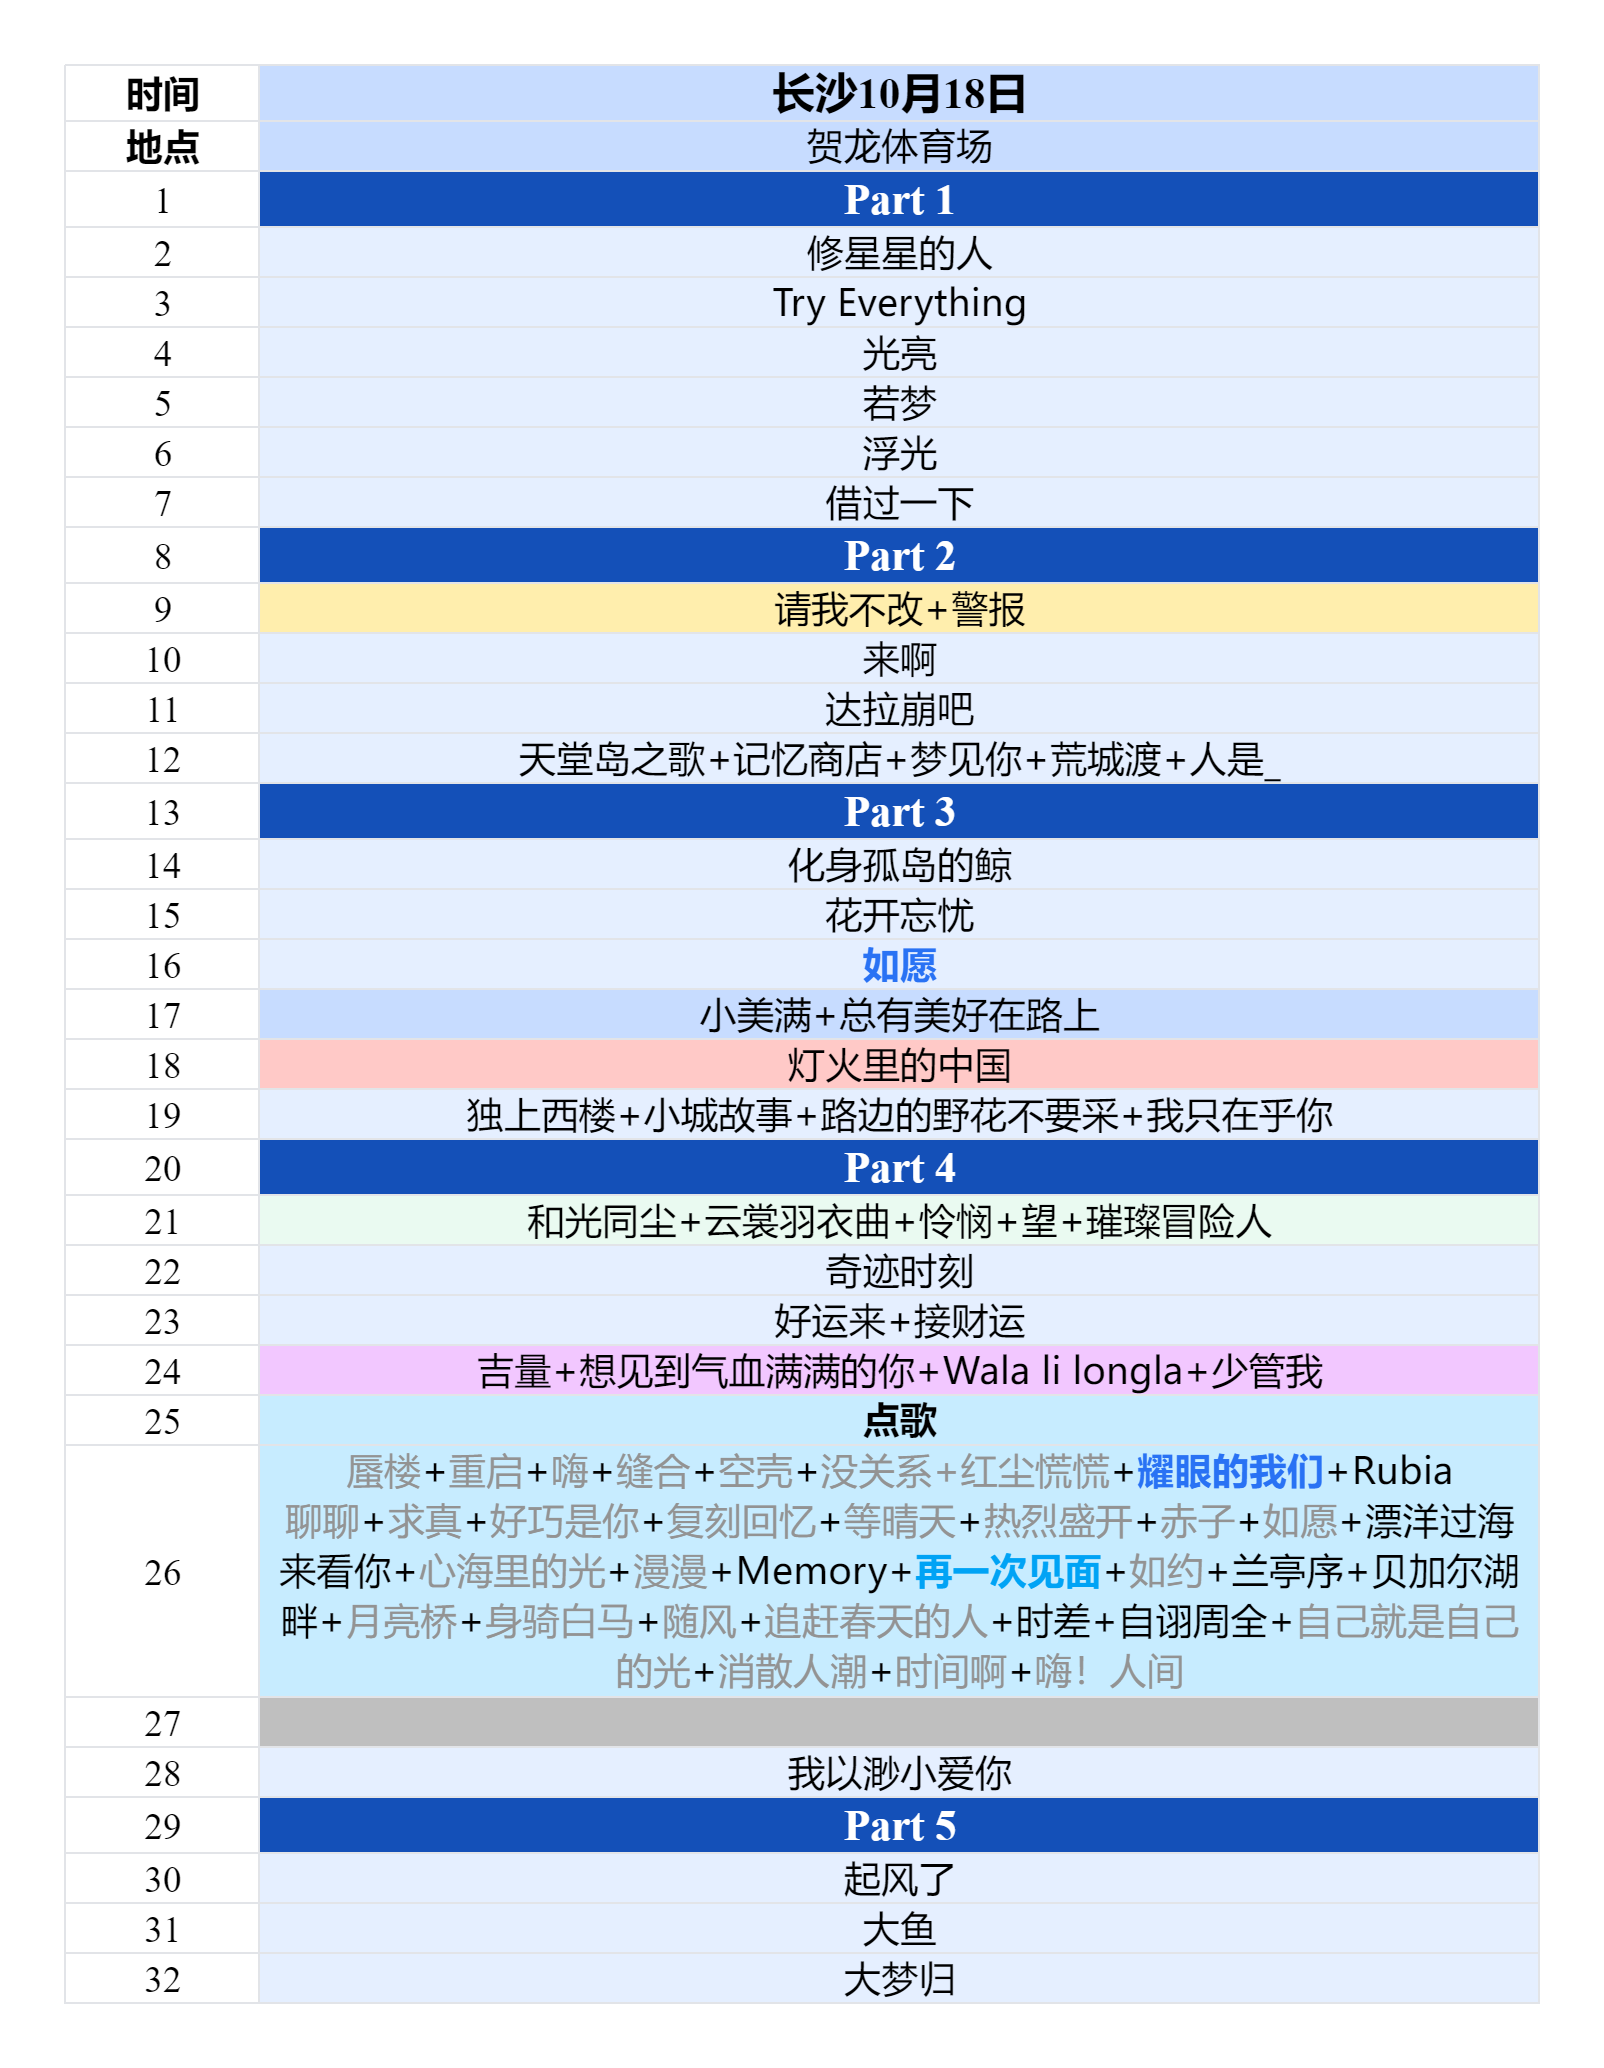
\includegraphics[width=280pt]{img/playlists/ChangSha-20261018} 

}

\caption{2026周深“深深的”巡回演唱会2026.10.18长沙场歌单}\label{fig:unnamed-chunk-55}
\end{figure}

\newpage

\section{Part1}\label{ChangSha-20261018-part1}

\hyperref[opening-vcr]{🎥【\textbf{开场VCR}】}（VCR 正文见附录 D。VCR 结束后《修星星的人》前奏直接响起。）

\hyperref[xiu-xing-xing-de-ren]{🎵【\textbf{修星星的人}】}（米：先声合唱：既然这宇宙让我诞生------）（深：是我在故乡的旷野，仰望银河的夏夜；是我在宇宙的风暴，朝着天仓五飘曳；我的孤独我的热烈，源自137亿年前，几粒星尘的蝴蝶；在噬星的幻灭里，为太阳撑一把雨伞；在时间的深海里，给地球道一声晚安〔首句现场听作''是我在故乡的光年''\,``朝着天堂的吊唁''，已按附录G校正，待核〕）长沙的朋友们你们好吗！（米：好------！）（深：既然这宇宙让我诞生，想必它是要以我为证〔现场听作''让我完整''，待核〕；我的情感和三十六度的体温，足以暖热即将熄灭的恒星；许我以造物的碎屑，重塑文明的边界；许我以渺小的羞怯，挽留物种的毁灭〔第二段主歌听写零散，已按附录G骨架整理，待核〕）（深：既然这宇宙予我重生，想必它是要让我看懂，我的基因和闪闪发光的记忆，足以照亮所有星际的永恒〔现场听作''的记忆曾闪闪发光的点滴''，待核〕）（高音吟唱）尖叫声（米：啊------！）

\hyperref[try-everything]{🎵【\textbf{Try Everything}】}长沙的朋友们，你们准备好了吗？既然宇宙让我们诞生，那就勇敢地 Try Everything，好不咯？（深：I messed up tonight, I lost another fight\ldots\ldots No I won't leave, I wanna try everything / I wanna try even though I could fail）尖叫声！（米：啊------！）（深：Look how far you've come, you filled your heart with love\ldots\ldots I'll keep on making those new mistakes / I'll keep on making them every day / Those new mistakes）你们好吗？到你们！（米：Try everything!）再大声！（米：Try everything!）再来一次！（米：Try everything!）Try everything\ldots{}

\hyperref[silver-linings]{🎵【\textbf{光亮}】}长沙的朋友们你们好吗？（米：好------！）长沙站第二场的朋友们你们好吗？（米：好------！）我都感觉我像换了一个城市开演唱会。昨天不是还热着，已经热得在冒汗了吗？怎么今天就已经\ldots\ldots 大家要记得加衣服好不好？（米：好------！）后面的朋友们你们好吗？（米：好------！）唉，虽然我是湖南人，但我是湖南邵阳的。我们湖南每个地方口音都不太一样，所以长沙话我其实真的也不太会说。但是我还是要说，给我一点鼓励好不好？（米：好------！加油！）长沙的朋友们，大家好，我是周深。好开心能够来长沙哒。谢谢你们来我的演演演演演唱会。〔口播结巴自嘲，听写待核〕长沙的宝哥、妹陀，你们好不咯？（米：好------！）长沙的\ldots\ldots 吃吃的\ldots\ldots 嗯\ldots\ldots 长沙的吃的\ldots\ldots 吃起来香喷喷，好韵味咯，是不咯？我只能用塑料普通话了。那大家一定要记得去多吃点好不咯？（米：好------！）有多少是我们长沙本地的朋友们？（米：哦------！）那有多少是跟我一样，就是从其他城市飞过来的朋友们呀？（米：哦------！）后面的朋友们呢，你们好吗？（米：好------！）一定要好好享受非常非常多的美食和美景好不好？那我就非常非常幸福了，因为我现在眼中看到的是全世界最美的风景，就是所有的光亮都汇聚在一起的模样。谢谢你们愿意成为我的光亮。（米：谢谢周深！）（深：海上一阵风吹起，白云涌向陆地，季风带走沙粒；四季冷暖的交替，多鲜活的生命，有枯萎的痕迹；是奔跑中突然袭来的风雨，是黑暗中一根火柴燃烧的光明；也许你猜不透未知的宿命，像流星飞翔着它却不知目的；可是啊，我却愿意，最渺小最微弱最柔软最无畏的你，用尽了全力，光亮你自己）我爱你。（戏曲念白＋唱腔两遍：莫听穿林打叶声，一蓑烟雨任平生；畅音阁里终一叙〔听作''畅饮过醉中离去，留半点音讯''，已按附录G校正〕，六百年一粟，沧海一梦）这边的朋友你们好吗？你们好吗？长沙的朋友们你们好吗？最无畏的你。

\hyperref[like-a-dream]{🎵【\textbf{若梦}】}等一下用最大的声音跟我一起唱若梦好不好？因为遇见你们这件事情美好的跟一场梦境一样哦。（深：浮生若梦，为欢几何；风摇雨落，此心何处停泊；剑起刀割，却斩不断这因果，看天地之间皆漠漠；尘缘萧索，宿命奈何；日升月落，此生依旧难舍〔听作''此生依旧停泊''，已按附录G校正〕；铁马金戈，也踏不碎这心火；忆前尘旧梦，任岁月消磨）到你们！（米：往事流转在你眼眸）哇！（米：一边遗忘一边拼凑；如我虔诚合十双手〔``如果前程何时相逢''听写已按附录G校正〕，唯愿你能得到拯救）长沙的朋友们唱得太好听啦！（深：情缘若梦，长久几何；一枕寒宵，饮下苦涩独酌；杯酒当歌，却绕不开这心锁；愿清欢入梦，伴此心停泊）再来！（深：往事流转，在你眼眸；一边遗忘）（米：一边拼凑）（深：如我虔诚）（米：合十双手）（深：唯愿你能）（米：得到拯救）全场最大声！（深：往事流转，在你眼眸；一边遗忘）（米：一边拼凑）（深：如我虔诚）（米：合十双手）（深：唯愿你能）（米：得到拯救）〔逐轮记录〕唯愿\ldots\ldots 长沙的满哥妹陀，能得到拯救。因为你们，周深才得到拯救。（米：欢呼声）

\hyperref[floating-light]{🎵【\textbf{浮光}】}〔本段前另有旁白：人生恍惚三万天，因为遇见了你，才值得留恋哦。一定要记得，你的存在非常非常有意义，好吗？（米：好！）〕（深：看指尖拨响蝴蝶，扇动一场离别；我推开无声岁月，续梦一页；你我只是打个照面，可曾有过誓约，走进熟悉却陌生的思念）啊\textasciitilde（深：你的眼眸装满了时间，你的身后拥故事成篇〔现场听作''永不是长夜''，已按附录G校正〕，此生如梦愿细数流年，与你同写沧海桑田；浮光掠影重山彩云间〔现场听作''重生在云间''〕，你的伏线穿越千百年〔现场听作''你的出现穿越千万年''〕，人生不过恍惚三万天，漫漫人间，留恋留连）你说那月光，吻过古渡和城墙，永恒的刹那的，此刻沉默无话可讲，想问你这星空，是否\ldots\ldots〔本曲后半现场唱词与附录G差异较大，已按附录G骨架整理，待核〕去吧去呀，总会相遇吧。一起！（米合唱：浮光掠影，转身再遇见〔现场版唱词，待核〕）再大声！（米合唱：你的出现，终结了孤单〔现场版唱词，待核〕）后面的朋友！（米合唱：感受过温暖，洒满人间〔现场版唱词，待核〕；慢慢了解，永远留恋〔现场版唱词，待核〕）（深吟唱：Ah\ldots{} Ah\ldots）（米：欢呼）（米：周深！好帅！〔旁人喊话，备注存档〕）

\hyperref[excuse-me]{🎵【\textbf{借过一下}】}（深：少年扬起脸庞，前往他的月亮，人们笑他狂妄，人怎可不一样；白衣过泥潭，怎敢说不染，但凡银两有价，谁能真潇洒；少年爬上城墙，去见他的月亮，破碎几次心脏，得来几句真相；市井或朝堂，四方皆如狂〔附录G作''如框''，已按附录G校正〕，若你生来有刺，磨掉再入场）你们都是对的，他说拜托，让开一下。（深：让我大醉一场，殿堂之上，背闲诗两三章；让我穿白衣裳，过疯人巷，去泥潭捞月光；望大人们见谅，提点的话，我懂也不想装；世人寻黄金乡，我找月亮，何必同往；话谢过，路借过，你是你，我是我）（深：正如先生所说，每颗心都有瑕；潇洒不是不怕，是愿付出代价）你们愿意吗？（米：愿意！！！）权衡利弊后，仍守对与错，谢过赐教的话，路借过一下。长沙的朋友你们好吗？（米：好！！！）（深吟唱：Oh\ldots{} Wu\ldots）长沙，最大的合唱声！（米合唱：让我大醉一场，殿堂之上，被现实凉三丈；都穿白衣裳，我逢人想，去你探老月光〔合唱听写已按附录G校正〕）再大声！（米合唱：碰打着门前梁，听见的谎，我痛也不想装〔附录G作''望大人们见谅，提点的话''，已按附录G校正〕）世人寻黄金乡，我找月亮，有你同往〔合唱听写，附录G作''何必同往''，待核〕。花谢过！你们！（米合唱：不结果。你是你，我是我。）再大声！（米合唱：花谢过，不结果。你是你，我是我。）（米合唱哼鸣：Wu\ldots{} Wu\ldots）（米合唱：拜托你一趟，是故里浪漫〔附录G作''白衣过泥潭，世故里浪漫''，已按附录G校正〕，是心有所安，不敢忘；人间多明暗，若天真犹在，当披上月光，走夜关〔``走夜晚''听写已按附录G校正〕）你们就是我要找的月光，我找到你们啦。（米：欢呼声、尖叫声）

\section{Part2}\label{ChangSha-20261018-part2}

\hyperref[robot-vcr]{🎥【\textbf{机器人VCR}】}（VCR 正文见附录 D。VCR 开篇日期句本场听作''二二二五年五月十七日。今天是我被选中执行任务的第两百天。系统维持正常运转的七万三千天''〔数字听写待核〕，其余与附录 D 一致。）

\hyperref[brave-heart]{🎵【\textbf{请我不改}】}（观众：周深！周深！〔齐呼〕）长沙第二站的朋友们你们好吗？（米：好------！）要比昨天唱得更大声好不好？（米：好------！）〔与《警报》连唱串烧，独立条目见下〕（深：请我不改）（米：嘿！）（深：我的姿态）（米：嘿！）（深：我的爱我的痛都与生俱来〔现场听作''都立正起来''，已按附录G校正〕；请我看开〔现场听作''请我摊牌''，待核〕）（米：嘿！）（深：我的存在）（米：嘿！）（深：我的明我的暗都不必躲开〔现场听作''我的命我的运''，待核〕；我原谅我自己，捡起遗憾拥抱无奈〔现场听作''也记得拥抱我无奈''〕；我允许我放手，让我勇敢活在现在〔现场听作''我必须我放手''〕；我不等待）（米：嘿！）（深：我不徘徊）（米：嘿！）（深：我的笑我的泪都不再苍白，放肆盛开）Break out!（米：Oh oh）Break out!（米：Oh oh）Break out!（米：Oh oh）（深：我发送警报声，血红色惊叹号，提醒你自救〔现场听作''摩擦声警报声''〕；被遥控，被惶恐〔附录G作''被耗空''〕，快失控，快冷冻〔附录G作''快断送''〕，我替你颤抖〔附录G作''我替你看透''〕；从激动到冰冻〔附录G作''从借用到利用，到享受到滥用''〕，转身就走，他们绝不为〔你〕回头〔附录G作''为你而痛''〕〔本段现场演唱版听写与附录G差异大，已按附录G骨架整理，待核〕）（深：是谁不断日夜合围，向我追来，痛击我最脆弱短板；是谁模糊我的未来，恐惧淹没了期待；绝望已经大军压境，回声却没办法认领〔附录G作''回身却没半个人影''〕，才看清决定与逃避〔附录G作''追兵与逃兵''〕，竟都是我自己〔本段现场版听写与附录G差异处已照词校正，待核〕）（尖叫声）（VCR：警报声〔间效〕）〔副歌多轮，``孤独的在深夜里，遗落计算，还能撑多久；越倔强越不容，越自己，最后就沦为败寇；低低头皱眉头，到最后不抬头，笑容失守''等尾段听写与附录G差异大，已按附录G骨架整理（附录G：``我不怕这一生因为你不知还能撑多久\ldots\ldots 我学会痛，为你而痛''），待核〕（深：请我不改\ldots\ldots 坦荡痛快）（音乐结束，观众欢呼）

\hyperref[jing-bao]{🎵【\textbf{警报}】}〔与《请我不改》连唱串烧〕（深：我发送警报声，血红色惊叹号，提醒你自救；被遥控被耗空，快失控快断送，我替你看透；从借用到利用，到享受到滥用，转身就走，他们绝不为你而痛）〔本曲现场演唱版听写与附录G差异大（``摩擦声警报声''``从激动到冰冻''等），已按附录G骨架整理，详见上条标注，待核〕

\hyperref[lai-a]{🎵【\textbf{来啊}】}有稍微暖和一点吗？（米：有------！）我知道很多就是可能朋友都是I人，然后或者是哪怕你很E，在平时工作的生活场景当中也很难突然''啊''大叫一声。但在演唱会可以。所以我想听一下最大的，试一下啊。试一下啊。嗯嗯。还还没开始呢。来，三二一，最大的声音！（米：全场最大分贝尖叫欢呼）真好。这样你们就不会保持着清亮的嗓音走出深圳的巡回演唱会了。〔口播''深圳''疑为口误或听写误，应为''深深''，待核〕要不然我会很没有面子哦。那接下来这首歌想要大家配合我一起唱一下，这首叫《来啊》。好不？（米：好！）你们要帮我配合唱的地方是当我唱''Don't tell me''，你们要''来啊啊啊啊啊，来啊啊啊啊啊''。试一下哦。Don't tell me（米：来啊啊啊啊啊，来啊啊啊啊啊！）还有人没学会哦。没学会没关系呢，我也不敢说什么。〔玩笑〕Don't tell me（米：Lie lie lie lie lie）还是求求你们最好学一下。行，那试一下。Don't tell me（米：Lie lie lie lie lie）那这首歌就靠你们咯。（深：我，我怎么就这样呆头呆脑，一不小心落入圈套，沉迷在神魂颠倒，Pass off，这灵魂乱七八糟〔现场听作''My soul''，已按附录G校正〕；我，瞳孔里都是你迷人的笑，越靠越近我越浮躁，神涣散虚无缥缈〔现场听作''神魂丧失多缥缈''，已按附录G校正〕，Can't stop，躁动在纷纷扰扰〔附录G作''躁动太纷纷扰扰''〕；天生的怪胎）（米：Me）（深：踌躇着徘徊〔现场听作''出场的坏''，已按附录G校正〕）（米：Me）（深：太嘈杂的时代〔现场听作''别草草的时代''，已按附录G校正〕）（米：Me）（深：1v1较量打乱了节拍〔现场听作''预备起较量打闹的节拍''〕）（米：Me）（深：别气急败坏）（米：Me）（深：别着急淘汰）（米：Me）（深：一万种防备阻碍，不如就算了靠过来；将错就错，别拖Let's go〔现场听作''别走''，已按附录G校正〕，随你操控）到你们！Don't tell me（米：Lie lie lie lie lie Lie lie lie lie lie）我望眼欲穿你别闪躲。再来！Don't tell me（米：Lie lie lie lie lie Lie lie lie lie lie）要爱就爱放纵吧别退缩。Don't tell me（米：Lie lie lie lie lie Lie lie lie lie lie）我倾尽所有赴汤蹈火。还有！Don't tell me（米：Lie lie lie lie lie Lie lie lie lie lie）敢不敢直视我，Let's go〔现场作''Let's fall''两读，附录G作''Let's fall''，待核〕。〔两轮〕\textbf{\textcolor{red}{我爱你们}}！哦好厉害你们学得好会啊。你们学得好快啊，我在说什么？〔口播听写待核〕Don't tell me（米：Lie lie lie lie lie）不准说谎哟，所以你们喜欢听歌手周深唱歌吗？（米：喜欢！）我不信，哈哈，好啦开玩笑啦。

\hyperref[dalabengba]{🎵【\textbf{达拉崩吧}】}那接下来这首歌呢是很多朋友可能第一次听到歌手周深唱歌，也是在我们湖南卫视歌手上面当打之年被大家听到的舞台叫做《达拉崩吧》。〔《歌手·当打之年》湖南卫视梗〕也是我们深深的巡回演唱会的一个小游戏环节。不要期待今天的小腹肌没有带哟。〔玩笑〕那这个游戏环节就是每个人可以根据你喜欢的颜色去变换你的荧光棒。呜，好冷啊今天。大家可以分别换你们喜欢的颜色，蓝色、黄色、粉色或者是绿色。请注意只有蓝色、黄色、粉色或者是绿色，好吗？没有红色。红色的朋友应该是想保护一下嗓子对不对？〔玩笑〕选择不同的颜色代表你们选择不同的角色，分别蓝色是达拉崩吧，黄色是国王陛下，粉色是公主米娅，那绿色就是恶龙。他们都有相对应的台词，所以当我喊到你的名字就要喊出他们的台词。我们来试一下，达拉崩吧！（米：我最棒！）国王陛下！（米：再说一次！）公主米娅！（米：救我啊！）恶龙！（米：嗷！）红色的朋友们准备办〔口播听写待核〕，怎么\ldots 红色的朋友们我们怎么办呢？（米：宝贝！）除了喊宝贝你们什么都可以。〔玩笑〕那不如我教你们一句长沙话。哇刚才说成\ldots 哎呀，我凭什么要教大家长沙话？不管了，有一句''哦该咯''，好不好？（米：好！）哦该咯。那就当我喊到''长沙''你们就喊''哦该咯''，好不好？（米：好！）就当我求你们了。（米：好！）长沙！（米：哦该咯！）你刚才不是答应我喊了''哦该咯''？你喊了''哦该咯''是吧？嗯。那只有一个人喊了''哦该咯''也不好吧。长沙！（米：哦该咯！）根本听不见''哦该咯''。达拉崩吧！（米：斑得贝迪！〔长沙场人名接龙〕）国王陛下！（米：哎呦喂！）公主米娅！（米：莫得法！）恶龙！（米：啊呜！）长沙！（米：哦该咯！）达拉崩吧！（米：斑得贝迪！）国王陛下！（米：哎呦喂！）公主米娅！（米：莫得法！）恶龙！（米：啊呜！）恶龙！（米：啊呜！）恶龙！（米：啊呜！）恶龙！（米：啊呜！）长沙！（米：哦该咯！）长沙！（米：哦该咯！）恶龙乘以十，走！（米：啊呜！×10）多了一下。〔口播听写待核〕长沙！（米：哦该咯！）求你们了，那我们一起来唱《达拉崩吧》吧。（米：好！）（深：很久很久以前，巨龙突然出现，带来灾难，带走了公主又消失不见；王国十分危险，世间谁最勇敢，一位勇者赶来大声喊：我要带上最好的剑，翻过最高的山，闯进最深的森林，把公主带回到面前；国王非常高兴，忙问他的姓名，年轻人想了想，他说：陛下我叫，达拉崩吧斑得贝迪卜多比鲁翁；再说一次，达拉崩吧斑得贝迪卜多比鲁翁；是不是，达拉崩吧斑得贝迪卜多比鲁翁；对对，达拉崩吧斑得贝迪卜多比鲁翁）还有小朋友。达拉崩吧！（米：斑得贝迪！）国王陛下！（米：哎呦喂！）公主米娅！（米：莫得法！）国王陛下！（米：哎呦喂！）恶龙！（米：啊呜！）达拉崩吧！（米：斑得贝迪！）长沙！（米：哦该咯！）（深：英雄达拉崩吧，骑上最快的马，带着大家的希望，从城堡里出发；战胜怪兽来袭，获得十二金币，无数伤痕见证，他慢慢升级；偏远美丽村庄，打开所有宝箱，一路风霜伴随，指引前路的圣月光；闯入一座山洞，公主和可怕的巨龙，英雄拔出宝剑，巨龙说：我是昆图库塔卡提考特苏瓦西拉松；再来一次，昆图库塔卡提考特苏瓦西拉松；是不是，昆特牌提琴烤蛋挞苏打马拉松；不对是，昆图库塔卡提考特苏瓦西拉松）达拉崩吧！（米：斑得贝迪！）国王陛下！（米：哎呦喂！）公主米娅！（米：莫得法！）恶龙！（米：啊呜！）长沙！（米：哦该咯！）达拉崩吧！全场一起！于是------（深、米：达拉崩吧斑得贝迪卜多比鲁翁）砍向（深、米：昆图库塔卡提考特苏瓦西拉松）然后（深、米：昆图库塔卡提考特苏瓦西拉松）咬了（深、米：达拉崩吧斑得贝迪卜多比鲁翁）最后（深、米：达拉崩吧斑得贝迪卜多比鲁翁）战胜了（深、米：昆图库塔卡提考特苏瓦西拉松）救出了（深、米：公主米娅莫拉苏娜丹妮谢莉红）回到了（深、米：蒙达鲁克硫斯伯古比奇巴勒城）（深、米：国王听说达拉崩吧斑得贝迪卜多比鲁翁，打败了昆图库塔卡提考特苏瓦西拉松，就把公主米娅莫拉苏娜丹妮谢莉红，嫁给了达拉崩吧斑得贝迪卜多比鲁翁；啦啦，达拉崩吧公主米娅，幸福得像个童话〔``他们生下一个孩子''段录音至此〕）达拉崩吧的全名是？（米：达拉崩吧斑得贝迪卜多比鲁翁！）这位男士你只张嘴一个字都没对。〔玩笑，口播待核〕那条恶龙的名字是？（米：昆图库塔卡提考特苏瓦西拉松！）你们是最好的芒果\ldots\ldots 啊，长沙！（米：噻！〔``嬲噻''省读，听写待核〕）阿木的全名是？（米：宝贝！）你们已经用''宝贝''来敷衍阿木的全名了。〔玩笑〕恶龙乘以十，走！（米：啊！×10）真棒。长沙！（米：嬲噻！）由念你来念，啊------尖叫上！〔口播听写待核〕（米：尖叫声）呜呼！

\hyperref[haven-song]{🎵【\textbf{天堂岛之歌}】}大家要记得随着天气去添加衣物哟好不好？你看我们也没有想到嘛，昨天这么热，我这今天这么冷的。好冷的，大家一定要记得加衣服哟。那在前年我发了一张专辑，那个专辑的名字叫做\ldots\ldots（米：反深代词！）《反深代词》。它是前年发的一张专辑，它说的是两百年后的事情，有个世界叫做''反深代词''。周深一共有十二个不同的情绪碎片，也就是那张专辑一共有十二首歌，所以你在听那张专辑的时候，你发现某一首歌跟你的情绪、跟你的经历简直一模一样的时候，那证明我们在''反深代词''那个世界，我们彼此相互拥抱安慰啦。俗称我们找到了彼此。所以求求大家去线上听一下这张专辑好不好？以及今年它的实体专辑也发行啦！有的朋友们跟我一样已经拿到了对不对？是不是还有朋友还在等啊？都拿到了？是不是还有很多朋友没有买啊？没事啦没事啦没事啦哈。〔口播玩笑〕那就线上也一样可以听这这张专辑好不好？后面的朋友听到了吗？听到了摇一下你们的荧光棒啊。呜呼！为什么刚才在歌里不摇啊？〔玩笑〕让我们来看一下，在《反深代词》的蜃楼当中，摇一下我看一下。谢谢大家来看我们。看一下在《反深代词》的蜃\ldots\ldots 再摇一下我看一下。看一下在《反深代词》的蜃楼当中，周深又遇到了什么样的故事吧。〔蜃楼VCR〕（有人在看着你，有人在看着你，有人在看着你。〔《天堂岛之歌》前置VCR片段，附录D未收录，建议补录；与前场不同，待核〕）（深：叮咚，我有一个秘密，悄悄告诉你，欢迎你来到天堂入口。叮咚，有人在按门铃，是谁在外面？把恶作剧当一场游戏。听啊谁在哭泣，看那谁在窃窃私语，窗外有双眼睛，他在时刻注视着你。叮咚，有人在看你的梦〔附录G作''看你的过去''，现场演唱变体，待核〕。叮咚，有人在看你的梦。叮咚，有人在看你的梦。你逃不出去）生米们，你们在哪？（米：啊------！）你逃不出去。你逃不出去。（米合唱：有客人从远方来，爱恨都落得明白〔附录G作''有客人从夜里来，买很古老的年代''，合唱听写待核〕，亲爱的我很抱歉，不说的没有了没人记得〔附录G作''不朽的没有了没人记得''〕，不说的没有了没人记得）

\hyperref[the-memory-store]{🎵【\textbf{记忆商店}】}刚才我鞋掉了就你笑得最大声。〔对伴舞互动小剧〕你也不是第一次在记忆商店打工了。是可以笑成这样的吗？这么庄严肃穆的时刻。你也笑了。哦！所以这是反身代词〔口播沿误，即《反深代词》〕里面的记忆商店对不对？（米：对！）我们现在在的是深深的巡回演唱会。我在梦里面见过这样相同非常美丽的场景。他们都说梦都是相反的。在梦里面我跟他们对暗号，怎么都对不上嘞。我相信在现实一定对得上的对不对？（米：对！）看看，你们说对的时候不心虚吗？〔玩笑〕长沙！（米：嬲噻！）梦想成真啦。（米：哇------！）哦，只要用这一颗米子心，就可以唤醒记忆商店里面你最喜欢想要购买的那一段回忆。但跟你们相遇的每一分每一秒，都是我最幸福的时刻。那就选刚才笑的\ldots\ldots 最小声的这一段回忆吧。一时间找不出来谁没有笑呢。〔气球互动小剧，听写待核〕〔唱段听写不清，唱词见附录G《记忆商店》，待人工补录〕

\hyperref[meng-jian-ni]{🎵【\textbf{梦见你}】}（深：看着眼前还年少的你，恍如流年从未淌过去；时光飞逝就算我已经老去，你却仍有着初见时那双清澈的眼睛；当再一次听你喊出我姓名，就已将一生都历经，明白有些事情早注定；我们都站在时间的河里，离别是相遇的倒影；从初问候的那天起〔附录G作''从初吻后的那天起''，待核〕，就有了再见的伏笔；我望着你远去的背影，渐行渐远直到看不清；时间会改变一切，却再也无法改变你；若多年后还能够有幸，重逢在另一场梦境，但愿那时你在人海里，仍将我一眼认清）（米：不说的没有了没人记得〔合唱句待核〕×2轮）沙------长沙！（米：嬲噻！）这个气球不写字的原因是\ldots\ldots 因为你想比划长吗？不好笑。〔冷笑话互动，听写待核〕哎，你能不能给大家说一个冷笑话，如果让大家都给你鼓掌的话，那我们就一人一起捏爆一个气球好不好？如果不可以的话，那就\ldots\ldots 你自己捏爆两个气球吧。想好一个冷笑话。来给他一点鼓励。好，你自己捏爆两个气球吧。〔冷笑话失败，听写待核〕有啊。你每天在干什么？不好好练舞。（观众：呃，鬼来到了湖南。）第一个这个字怎么播出？好。（观众：这个来到鬼是\ldots\ldots 不是。）好。来到了，来到了哪里啊？（观众：湖南。）然后呢？（观众：呃，吃什么？）我不知道。（观众：周嫑嫑。）〔冷笑话内容为''嫑''字梗，完整文本听写待核〕为什么？允许我生气三秒钟。〔玩笑，听写待核〕

\hyperref[huang-cheng-du]{🎵【\textbf{荒城渡}】}（深：夜色中寻觅过，当往事困住我，也贪心中生出一点萤火〔附录G作''也盼心中生出一点萤火''〕；孤城的传说，有谁来过，将因果葬于我〔附录G作''将因果赠与我''，已按附录G校正〕；我在等着因果，渡魂渡魄渡我；纵然一世执着难舍，断了这心魔，可原谅我〔现场听作''可原谅么''〕；宿命中获得这解脱，重来过）（深：眼中风尘，手中残破〔附录G作''手中残魂''〕，那故事斑驳荒丘〔附录G作''斑驳荒城''〕；想念天真〔附录G作''修炼天真''〕，拨开心门，我亦可同谋这不舍〔附录G作''握一颗糖暖这孤身颠簸''〕〔本曲现场演唱版听写与附录G差异大，已按附录G骨架整理，待核〕）（米：我说他没有烂尾这一摊〔合唱句，或为''不朽的没有了没人记得''，听写待核〕×2轮）哦\textasciitilde（深：为这摊牌棋局〔附录G作''未知摊开棋局''，已按附录G校正〕，舍弃昨日才可破；再见了我的月光我的蓝我的爱；钢铁的巨兽在轰鸣，我们拒绝走入夜晚；破碎是新生的约定，我便愿为尘埃；让死亡觊觎我，让恐惧亲吻我，来摧毁我深爱的一切，可仍夺不走我的选择；弹指间湮灭我，但命运打不败活着；让生命如剧烈的烟火，璀璨熄灭前也将点亮，孩童的双眸；若巨浪已淹没了来路，我是帆亦是舟；是微渺的希望，我们依然前行，没有光指引）全场帮我一起唱！让死亡消亡我〔附录G作''让时空消亡我''，已按附录G校正〕------你们！（米：无需记得我）来摧毁我深爱的一切，可仍夺不走我的选择。再来！弹指间\ldots\ldots〔本曲后段副歌重复，已按附录G〕

\hyperref[Humans_are_]{🎵【\textbf{人是\_}】}（米：合唱〔录音此处欠清晰，副歌逐轮记录待人工补核〕）曾经我也以为，那些失去的、过去的，才是最完美的。但是因为遇到了你，听到你的歌唱，我才知道，我们现在拥有的每一分每一秒，才是最好的、最值得珍惜的。你们说，对吗？（米：对！）是你们创造了不朽的、永恒的爱。\textbf{\textcolor{red}{我爱你们}}！（观众：周深！宝贝！〔零星喊话〕）你们好啊！你们找到我了吗？（米：找到了！）你们出现在这里，我就知道，谢谢你们听到了我。（米：我们也听到了！）（深：我是只化身孤岛的蓝鲸，有着最巨大的身影。鱼虾在身侧穿行，也有飞鸟在背上停。我路过太多太\ldots\ldots〔唱词按附录G〕）

\section{Part3}\label{ChangSha-20261018-part3}

\hyperref[music-animations-vcr]{🎥【\textbf{音乐动画VCR}】}（VCR 正文见附录 D，本段为纯音乐动画，无旁白歌词。VCR 前后为纯音乐过场。）

\hyperref[The-whale-who-became-an-island]{🎵【\textbf{化身孤岛的鲸}】}谢谢你们。（米：周深！）你的衣衫破旧，而歌声却温柔，陪我漫无目的的四处漂流。我的背脊如荒丘，而你却微笑摆首，把它当成整个宇宙。你与太阳挥手，也同海鸥问候，陪我爱天爱地的四处风流。只是遗憾你终究，无法躺在我胸口，欣赏夜空最辽阔的不朽，把星子放入眸。到你们！（米：你的衣衫破旧，而歌声却温柔，陪我漫无目的的四处漂流。我的背脊如荒丘，而你却微笑摆首，把它当成整个宇宙。）大声！（米：你与太阳挥手，也同海鸥问候，陪我爱天爱地的四处风流。）后面的朋友！（米：只是遗憾你终究，无法躺在我胸口，欣赏夜空最辽阔的不朽，把星子放入眸。）（深：你的指尖轻柔，抚摸过我所有风浪冲撞出的丑陋疮口。你眼中有春与秋，胜过我见过爱过的一切山川与河流。曾以为我肩头，是那么的宽厚，足够撑起海底那座琼楼。而在你到来之后，它显得如此清瘦。我想给你能奔跑的岸头。）（米：没有墙头！〔应答提前，接墙头梗〕）这个高度换一个艺人来肯定是要撞到脑子的。〔对舞台装置玩笑〕你们到底有多少个墙头？（米：没有！）可能很多人不知道''墙头''是什么意思，因为我经常会问生米啊，就问歌迷朋友们，他们说：``你们都喜欢哪个歌手啊？''他们会说\ldots\ldots（米：欢呼声）哎，那我会说：``你们只喜欢歌手周深吗？''（米：是！）他们骗人的。〔玩笑〕所以呢，我就非常不礼貌地把他们喜欢的其他歌手称为''墙头''。所以这首歌就是问他们，你们到底有多少个墙头？（米：没有！）但是只要你们好好的成为自己，看到自己，无论怎么样，你们都是我的国王和王后。亲爱的朋友们，我们来长沙看你咯！你有好好的照顾好自己吗？（米：要！）一定要做到好不好？（米：好！）

\hyperref[Blossoms-that-forget-sorrow]{🎵【\textbf{花开忘忧}】}（深：巷子口买了花，穿过沿街红墙青瓦，夕阳慢慢亲吻着我的白发，推开旧木门回到家；把时光都炖香，而你只是笑不说话；一件遗憾的事就喝一碗汤，庭院深深秋叶飘落；我们苍老的时候就回到小时候，采青梅用来酿酒你不许偷着喝；穿朴素的衣裳牵着那衣袖，捡了小猫名为苍狗；我们睡去的时候像孩子无忧愁，反正也很难上锁这岁月如小偷；若记忆被偷走了忘了我的爱，我会说------）说什么？（米：你好啊！）你们好吗？（米：好！）（深：这是给你的花，花的名字叫忘忧草，他说时光汹涌如水上烟波，别走远了一起回家）我们一起回家好不好？（米：好！）谢谢你们的出现。（米：谢谢你！）没有你们就没有我。谢谢你们！（米：谢谢周深！）啊\ldots\ldots 我们一起------（深、米：我们苍老的时候就回到小时候，采青梅用来酿酒你不许偷着喝）（米：穿朴素的衣裳牵着那衣袖）（深、米：捡了小猫名为苍狗）大声！（深、米：我们睡去的时候像孩子无忧愁）（米：反正也很难上锁这岁月如小偷；若记忆被偷走了忘了我的爱；那永恒没骗我离散也没有，这份爱只是活在另外时空）（深、米：如果每一声再见会开启一个新的空间，每做一个梦是时空偶尔的重叠；你好吗离开的人啊，请帮我相爱到剧终）啊\ldots\ldots（深：忘忧草开着花，你在月光下不说话，一件遗憾的事就喝一杯茶，庭院深深秋叶飘落）在我们的生命当中，一定有那一个非常非常重要，也再也没有机会见到的人。但是我相信，只要我们的思念够大声，他就一定听得到。你们说，对吗？（米：对！）所以一定要好好的看见自己，照顾好自己，因为他也一定感受得到。对吗？（米：对！）花开忘忧，愿你无忧。花开忘忧！（米：愿你无忧！）谢谢长沙的朋友们！（米：谢谢周深！）谢谢你们。哦，来到我们长沙，那湖南好多好多歌都很适合在这里唱。昨天有一首大家唱的特别好听。（深：浏阳河）（米：弯过了几道弯）（深：几十里水路）（米：到湘江）（深：江边有个\ldots\ldots）〔《浏阳河》引子，接城市限定《如愿》导语〕

\hyperref[As-you-wish]{🎵【\textbf{如愿}】}长沙的朋友们真的唱得好好听啊，给自己一点掌声！那还有一首歌我觉得在这里也特别特别适合唱。就是大家非常熟悉的，非常熟悉的，但是呢不是我的歌。哦？猜一猜？因为我觉得爱这一个字，它应该是一个非常立体的一个字。我们要爱我们现在的繁荣昌盛的美好，也千万不要忘了我们曾经经历的那么多那么多的苦难，好吗？也像这首歌一样，希望我们每个人都一定要记住我们的来时路，才可以更好的珍惜我们的现在。希望每个人的愿望都可以如愿。在这里是不是好适合唱？等下大声跟我一起唱好不好？（深：你是遥遥的路，山野大雾里的灯。我是孩童啊，走在你的眼眸。你是明月清风，我是你照拂的梦。见与不见都一生与你相拥。而我将爱你所爱的人间，愿你所愿的笑颜。你的手我蹒跚在牵，请带我去明天。如果说你曾苦过我的甜，我愿活成你的愿。愿不枉啊愿勇往啊，这盛世每一天）不要忘了我们那些先辈们为我们遭遇的苦难，好不好？所以要更加的珍惜我们现在的每一分每一秒，好不好？（深：你是岁月长河，星火燃起的天空。我是仰望者，就把你唱成歌。你是我之所来，也是我心之所归。世间所有路都将与你相逢。而我将爱你所爱的人间，愿你所愿的笑颜。你的手我蹒跚在牵〔听作''跚在牵''〕，请带我去明天。如果说你曾苦过我的甜，我愿活成你的愿。愿不枉啊愿勇往啊，这盛世每一天。山河无恙烟火寻常，可是你如愿的眺望。孩子们啊安睡梦乡，像你深爱的那样）一起唱！（深、米：而我将梦你所梦的团圆，愿你所愿的永远。走你所走的长路，这样的爱你啊。我也将见你未见的世界，写你未写的诗篇。天边的月心中的念，你永在我身边。与你相约一生清澈，如你年轻的脸）

\hyperref[simple-bliss]{🎵【\textbf{小美满}】}那接下来，这一首歌，你们会唱吗？（米：会！）那让我听到我的第二场更大的声音好不好？（深、米：没什么大愿望〔现场与观众对唱版，附录G''没有什么事要赶''段现场听作''就什么事都敢想''\,``看到我就觉得勉强，也能笑得像太阳''，现场版唱词待核〕）唱！（深、米：乌云还挺大胆，顶在头上吹不散；我抓在手里捏成棉花糖，什么烦恼不能忘；既然是路一定有转弯，哪个风景都漂亮；揉揉疲惫的眼睛停下来看一看，美好简单）全场一起唱！（深、米：你看小狗在叫树叶会笑风声在呢喃，不如好好欣赏一秒迷迷糊糊的浪漫；只要一觉醒来床单洒满阳光的温暖；不去想不必想，不用急急忙忙说一个答案）再大声！谢谢你们！（米：谢谢周深！）（深：笑一笑就灿烂）唱！（深、米：唱一支歌就舒展，收集一点一滴小美满，都是幸福的花样；没道理的开朗）怎么了？〔口播听写待核〕（深、米：打扮平凡的日常〔现场听作''打发平凡的日常''〕，找到自己最合身的衣裳，只要自己够喜欢；至少还有温柔的眼光，还在夜里看月亮，心情铺得再满也要留一扇天窗，岁月很长）我们慢慢走好不好？〔口播〕（深、米：你看小狗在叫\ldots\ldots 不用急急忙忙说一个答案）亲爱的朋友们你们好吗？（米：好！）后面的朋友你们好吗？（米：好！）

（许愿环节）让我们一起在你创造的小美满当中许愿好不好？请相信相信的力量，请相信美好的力量。我给大家打个样哦，就像我这样，闭上眼睛，想好你要许的愿望。我会倒数三个数字，3、2、1，睁开眼睛，我们的愿望就会出现在这棵许愿树上。请相信相信的力量，现场的所有朋友，闭上眼睛，许愿喽。无论什么年龄段，无论什么职业，闭上眼睛，想一想你生日的时候第一个蹦出来的愿望是什么呢？想一想你一直想要实现的愿望是什么呢？哦，对了，在小美满这首歌当中的愿望，有一个要求，只能够许关于自己的愿望。想一想，是不是自己在忙碌在很多的角色当中，却忘记看一眼自己呢？是不是很久没有跟自己说一声，你真的辛苦了？3、2、1，睁开眼睛！（深、米：你愿相信什么就把世界看成什么样，偶尔难题加点重量越要轻轻地旋转，所以无论如何记得保管小小的光环；笑就好哭也好，今天就是明天最好的陪伴）你们唱！（米：今天就是自己最好的陪伴！〔现场合唱改词，待核〕）你们都是终身最好的陪伴。〔口播，或作''周深最好的陪伴''，待核〕这个世界因为你的诞生变得更加美好，每一天也因为你而变得非常非常特别。让我们祝今天过生日的朋友！（米：生日快乐！）让我们祝昨天或者是前一段时间过生日的朋友！（米：生日快乐！）让我们祝明天或者过一段时间过生日的朋友！（米：生日快乐！）因为看见了你啊，我才看见\ldots\ldots{}

\hyperref[zong-you-mei-hao-zai-lu-shang]{🎵【\textbf{总有美好在路上}】}（深、米：花在开，云在飘，笑容在脸上，我们向前方一路向阳）你们！（深、米：亲爱的你，在路上呀，也在看海呀〔附录G作''在路上慢慢逛，看一看太阳''，现场版唱词待核〕。让风轻轻，吹拂你的脸庞。今天过去，还会有明天和后天呀〔附录G作''要到明天看看天气会怎样''，现场版唱词待核〕；烟火晴朗，故事都慢慢长〔附录G作''阴或晴朗，故事都慢慢赏''，现场版唱词待核〕）抬头发现，你们就是光芒。谢谢你们！（米：谢谢周深！）

\hyperref[deng-huo-li-de-zhong-guo]{🎵【\textbf{灯火里的中国}】}灯火里的中国美不美？（米：美！）那是因为最美好的你一起组成的哟。等一下跟我大声的唱好不好？（米：好！）（深、米：都市的街巷已灯影婆娑，社区暖暖流淌的欢乐。远山的村落火苗闪烁，渐渐明亮小康的思索。归港的船帆从灯塔掠过，追梦脚步月下交错。广场焰火在节日诉说，星空升腾时代的巍峨。灯火里的中国，青春婀娜。灯火里的中国，胸怀辽阔。灯火漫卷的万里山河，初心换回了百年承诺。灯火里的中国，青春婀娜。灯火里的中国，胸怀辽阔。灯火灿烂的中国梦，灯火荡漾着心中的歌）等下跟我大声唱好不好？（米：好！）（深：归港的船帆从灯塔掠过，追梦脚步月下交错。广场焰火在节日诉说，星空升腾时代的巍峨）你们唱！（米：灯火里的中国，青春婀娜。灯火里的中国，胸怀辽阔。灯火漫卷的万里山河。初心换回了百年承诺。）最大声！（米：灯火里的中国，青春婀娜。灯火里的中国，胸怀辽阔。灯火漫卷的万里山河。初心换回了百年承诺。灯火荡漾着心中的歌。灯火荡漾着心中的歌。）〔听写待核〕你们唱的太好听了，我还想再听一次哦。（米：灯火里的中国，青春婀娜。灯火里的中国，胸怀辽阔。）（深：灯火漫卷的万里山河。）（米：初心换回了百年承诺。）再来一次！（米：灯火里的中国，青春婀娜。灯火里的中国，胸怀辽阔。灯火灿烂的中国梦。灯火荡漾着心中的歌。）太棒了！灯火荡漾着心中\ldots\ldots（米：的歌。）给自己掌声！

（摄影师魔术环节）我跟你们说哟，我不仅会变魔术，你先站住。〔拦住摄像师〕我们这位摄像大哥都不去研究摄像机器和摄像技术了，有一天我发现他也会变魔术。但是我们的时间很宝贵，我给你一分钟可以变完吗？一分钟，变完你准备的魔术。那我拍你哦。讲个笑话，我不要讲笑话。太冷了，今天天气挺冷的。掌声我们看一下他的魔术。需要互动的那种类型是吗？哦你在上面一个台阶跟我一起说话礼貌吗？〔玩笑〕哦这是扑克牌我可以检查吗？我可以啊。大家看没有问题对不对？好。（摄像师：呃你帮我选一张。）那我就旋转然后你们一直停好不好？你们帮我五、四、三、二、一，我听到一我就停。五\ldots\ldots（米：五四三二一！）要抽出来吗？你不要看到对不对？你不能看到。我最珍贵的观众朋友们可以看到吗？那你先闭眼睛，你闭眼睛哦，你闭眼睛，闭眼睛啊！不要抬头了你还是睁开的，闭眼睛啊。悄悄的啊。好，怎么了？啊你们没看到？你再闭一下眼睛。说好了一分钟光聊天一分钟都已经过去了。看到了吗？好，然后嘞？（摄像师：帮我放进牌堆里面。）哈，那我们拿出来干嘛？闭眼睛闭眼睛，闭眼睛闭眼睛你闭眼睛你闭眼睛。有问题，好，一分钟过去了，好然后嘞？（摄像师：在背后可以找到你要的。）哦就卡在手指的刚才那个地方是吗？好来吧来来来。（摄像师：我会把它弹出来，有一张。）哦特写一下哦，哦唯独是我刚抽的那张对。掌声！那等一下我变的魔术如果失败了怎么办？〔口播听写待核〕我们歌手周深会继续好好唱歌的，因为我可以用歌声陪伴你们对不对？也希望我可以像邓丽君女士一样，可以唱好多好多歌，成为你们的时间胶囊，到时候你们在听到这首歌的时候我们又彼此相互\ldots\ldots 我拥抱了，对不对？（米：对！）那如果等下你会唱，跟我一起大声唱好不好？（米：好！）

🎵【\textbf{邓丽君组曲}】

\hyperref[du-shang-xi-lou]{🎵【\textbf{独上西楼}】}（深：无言独上西楼，月如钩。寂寞梧桐，深院锁清秋。剪不断理还乱，是离愁）你们的墙头\ldots\ldots（米：没有！）（深：是不是你们的墙头？）（米：没有！）（深：别有一番滋味在心头）

\hyperref[xiao-cheng-gu-shi]{🎵【\textbf{小城故事}】}我们现在在哪座城市？（米：长沙！）（深：长沙故事多〔现场改词〕）（米：唱过一支歌〔或作''充满喜和乐''，合唱听写待核〕）（深：若是你到长沙来〔现场改词〕，收获特别多）有哪些收获？（米：看似一幅画）（深：听像一首歌）后面的朋友大声唱！（深、米：人生境界真善美，这里已包括。谈的谈说的说，你们的墙头真的多〔现场改词〕）（米：没有！）（深：请你的朋友一起来）在哪里？（米：长沙来做客）你们来邀请。（深：请你的朋友一起来）来哪里？（米：长沙来做客）

\hyperref[donot-pick-the-roadside-flowers]{🎵【\textbf{路边的野花不要采}】}这首歌会唱吗？（米：会！）听到你的声音。（深：送你送到小村外）（米：有句话儿要交代）（深：虽说\ldots\ldots）（米：路边的野花\ldots\ldots）那些墙头多的人要注意了哟。〔口播〕路边的野花------它怎么啦？（米：不要采）那就大声的唱出来吧！（深：记着我的情）（米：记着我的爱）（深：记着有我天天在等待。我在等着你回来）唱！（米：千万不要把我来忘怀）（深：千万不要把我来忘怀）（深：千万不要把我\ldots\ldots）怎么了？（米：来忘怀！）谢谢你们！（米：谢谢你！周深！）我时常在想，如果没有被你听见，没有被你看见，我现在在做什么呢？谢谢你们的善意，谢谢你们的爱。

\hyperref[I-only-care-about-you]{🎵【\textbf{我只在乎你}】}（深：如果没有遇见你，我将会是在哪里。日子过得怎么样，人生是否要珍惜）唱！（米：也许认识某一人）（深：过着平凡的日子）（米：不知道会不会）（深：也有爱情甜如蜜。任时光匆匆流去，我只在乎你，心甘情愿感染你的气息）大声唱！（米：人生几何能够得到知己）（深：失去生命的力量也不可惜。所以我求求你，别让我离开你，除了你我不能感到一丝丝情意）〔合唱逐轮记录；全曲大合唱〕

\section{Part4}\label{ChangSha-20261018-part4}

\hyperref[mask-vcr]{🎥【\textbf{面具VCR}】}（VCR 正文见附录 D。开篇日期行本场为''2026年10月18日，长沙''，其余与附录 D 一致。）

（米：对！）〔回应 VCR 结尾''你说，对吗？``〕我没听到哦，你说，对吗？（米：对！）你们会大声地跟我一起合唱，对吗？（米：对！）

\hyperref[stay-with-light]{🎵【\textbf{和光同尘}】}（合唱：和你一起歌唱，和你一起唱〔附录G作''和你一起歌，和你一起合''，合唱记法待核〕。月落星沉，日出东海）（合唱：和你走过，理想的大海〔附录G作''理想的大河''，已按附录G校正〕）（合唱：汹涌的，被灌溉〔附录G作''从容的，沸腾着''，已按附录G校正〕）（深：你看那盛放的花，来自期盼的种子。你看那丰硕果实，来自耕耘的浪漫。宽广的大河，来自八方汇聚的小溪。奔腾向前的大江，来自高山的哺育。和光同行，跌跌撞撞的摸索。和光同舞，奋不顾身的坎坷。和光同尘，不为盛名而来〔现场听作''不为生命而来''，已按附录G校正〕，不为低谷而去。和光同尘，为你而来，有你，我在）

\hyperref[Song-of-the-cloud-dress]{🎵【\textbf{云裳羽衣曲}】}我们的缘分一定不会太浅，因为我的名字叫------（米：周深！）因为我们的巡演的名字叫------（米：9.29Hz！〔观众以2024巡演名应答，待核〕）大声唱好不好？（深：故事鲜艳，而缘分却太浅〔听作''不是鲜艳''，已按附录G校正〕）（米：我的爱恋，竟如此的明显）（深：摸不清的默念〔附录G作''我不停地默念''，已按附录G校正〕，想牢记你的容颜）大声唱！（米：不眠的思念，你又在〔附录G作''故事鲜艳，而结局却搁浅''，已按附录G校正〕）这些年你又在哪座红尘之间，幻化成哪张脸。（深：云袖之间月下拨弄琴弦〔附录G作''你轻落指尖''，已按附录G校正〕，一曲吟唱月夜明〔附录G作''一曲云裳羽衣恋''，已按附录G校正〕，人世间，漫天飞舞着思念）愿化作曾经的相遇，在你身边。〔现场版结尾唱词，待核〕

\hyperref[lian-min]{🎵【\textbf{怜悯}】}（深：我要比你显得更无情）（米：来生里长亭，月明时抛来的公平〔现场应和句，附录G无对应，听写待核〕）（深：我要带着恨意等着你〔附录G作''带着爱意恨着你''，已按附录G校正〕）（米：风眼中没我你最行〔现场应和句，听写待核〕）（深：我要抱着玉净树聆听，辗转掌心〔现场应和句，听写待核〕；打碎了天边云，说非你，天意从未见〔现场应和句，听写待核〕）〔唱段听写不清，唱词见附录G《怜悯》，待人工补录〕我们不要祈求怜悯，我们不要生病对不对？（米：对！）我们每个人都值得被好好的爱着，对不对？（米：对！）

\hyperref[Expectation]{🎵【\textbf{望}】}我们总会绕啊绕，绕啊绕（米：绕啊绕，绕几千里路也望向归途）（深：乘着风，想念吹拂，游夜空漂浮，抓一颗流星做礼物，愿你幸福。手中线，绕啊绕，绕啊绕）（米：绕啊绕，绕几千日夜也望向归途）（深：燕归巢，迁徙之路，参与者无数，待到烟火照夜白时，准备庆祝。我们心有所住）大声！（深：我们总会绕啊绕，绕啊绕）（米：绕啊绕，绕几千里路也望向归途）（深：乘着风，思念吹拂，游夜空漂浮，抓一颗流星祝福，你要幸福。手中线，绕啊绕，绕啊绕\ldots\ldots）〔多轮逐轮记录〕

\hyperref[adventurers]{🎵【\textbf{璀璨冒险人}】}（深、米：他们说要越过前方风沙必须低着头，他们说要绕过蜿蜒的河才能往前走。他们说烫要放手，太远要换个路口，如果得不到谁的认同，那就不算拥有。没人能够决定谁的一生应该怎么活，没人能够定义谁的天空是什么颜色。没人未梦就先懂，只是单纯相信着，背向光的英雄，每张轮廓出自平凡的沉默）你们就是我的英雄！（深、米：沿途一身泥泞跌撞的是我，忍痛缓行不回头的也是我〔听作''忍痛换醒''，已按附录G校正〕。就让一路曲折每一道伤口，洗净我的脆弱。原来咽回去的泪，才能淹没了脆弱，你发誓更勇敢一生与梦相拥〔听作''相拥着''〕。还想要继续吗？要逆风不退啊，让痛苦住进你眼眸。别怕未来的模样，辜负曾经的凝望〔听作''不负''，已按附录G校正〕。有多少理想就有多少次传唱〔听作''穿肠''，已按附录G校正〕，那沿途的风浪，也不过就这样，这一路光景有你们在身旁。要真的爱〔附录G作''要炙热啊''，现场版唱词，待核〕，要不麻木〔附录G作''要不枉啊''〕，要有锋芒〔附录G作''要勇往啊''〕；起风了，不管了〔附录G作''呼唤了''〕，你还在等什么；挥手了，再见了，别不舍回头啊，向心中的梦啊，去追吧）（深：要多少伤痕才算磨破〔附录G作''才算活过''〕，愿你记得，愿你哭过，不惧脆弱。不惧脆弱。不惧脆弱。〔现场重复〕）希望你永远无畏，也不害怕面对自己脆弱的那一面，好吗？（米：好！）因为脆弱的一部分也是组成最完美的我们的一部分，你们说对不对？（米：对！）愿你勇往直前，也------（深、米合唱：不惧脆弱）以前我都不敢开口唱歌，因为我感觉声音非常奇怪。但是因为遇见了你，每一分每一秒都叫做奇迹时刻！

\hyperref[miracle-moment]{🎵【\textbf{奇迹时刻}】}（深：若相信谁都可以重塑现在，不需要等待Show time，此刻就无限精彩。I wanna see my way in starlight，奇迹时刻等你一起来，开启夺目现在。We gonna change the fate never deny，以无数颗渺小的光彩，就能照亮无穷未来\ldots\ldots 以最单纯魔力和热爱〔听作''茉莉花的爱''，已按附录G校正〕，就能一起冲破阻碍。别管这错综的光影，现实永远有意外，一根丝线就能牵动星球离开。如果要找回自己，线索在九霄云外，无论要去多远的宇宙，Here we go。你们好吗？（米：欢呼声）这世界总有太多无理光怪〔待核〕，一起起会期待〔附录G作''以惊喜回应期待''，待核〕\ldots\ldots）〔本曲前段在转写稿中与上曲衔接，唱词已按附录G校正〕掌声欢迎我要变魔术啦！（米：欢呼声、掌声）（笑声）再给我点鼓励！（米：欢呼声）【魔术环节】大家有看到这是四个那个很普通的铆钉对不对？（米：对！）哎哟，没问题啊。这是一个非常普通的木板对不对？（米：对！）这是一张非常普通的纸对不对？（米：对！）那正常这样放过去，它是没有办法粘住的对不对？（米：对！）我现在拿一个红色的铆钉，我把它钻进去。按道理来说我这样扯的话，它可以扯开吗？（米：不能！）帮我倒数三个数字。三、二、一！（米：观众惊呼）厉不厉害？（米：厉害！）为了让你们看到没有任何问题，我们现在把红的这个拿出来，是不是没有任何问题？（米：是！）还有一个魔术哦，这是三个骰子对不对？没有任何问题吧？（米：没有！）来看一下哦。我现在随便摇一个数字。这是几？（米：五！）我把它放进去没有任何问题对不对？（米：对！）然后我现在随便再把它放一个放到这儿。（米：观众惊呼声）大家看一下，来特写。它没有\ldots\ldots 没有问题吧？这是几？（米：六！）但是只要你们给到我欢呼声之后，来，三、二、一！（米：观众欢呼）它就变成了\ldots\ldots（米：观众欢呼）这是几？（米：八！）来，三、二、一！（米：观众欢呼）〔骰子魔术〕好运来了大家接不接？（米：接！）

\hyperref[good-fortune-comes]{🎵【\textbf{好运来}】}（深：好运来祝你好运来，好运带来了喜和爱，好运来我们好运来）恭喜发财接不接？（米：接！）（深：迎着好运兴旺发达通四海）就是降幸福呀，你们接不接？〔口播听写待核〕（米：接！）（深：叠个千纸鹤再系个红飘带，愿善良的人们天天好运来；你勤劳生活美，你健康春常在\ldots\ldots）〔后段与前场体例同，多轮合唱逐轮记录〕长沙的朋友们你们好不好？（米：好！）那接下来，用最大的声音，跟我一起接所有最美好的祝福好不好？（米：好！）准备好了哟，我要听到你们的声音。我们一起接平安，你们------（米：接平安！）接幸福！（米：接幸福！）接健康！（米：接健康！）接好运！（米：接好运！）接不接？（米：接！）（深、米：好运来祝你好运来，好运带来了喜和爱；好运来我们好运来，迎着好运兴旺发达通四海；叠个千纸鹤再系个红飘带，愿善良的人们天天好运来；你勤劳生活美，你健康春常在，你一生的忙碌为了笑逐颜开；打个中国结，请春风剪个彩，愿祖国的日月年年好运来；你凤舞太平年，你龙腾新时代，你幸福的家园迎来百花盛开）〔深唱句与米合唱逐句对唱记录〕长沙的朋友，祝你们恭喜发财！（米：恭喜发财！）接不接？（米：接！）你们说我敢吃这个辣椒不？（米：敢！）你们都说我敢吃了，那我就不吃了。〔玩笑〕吃的，让我听到你们的欢呼声。（米：啊------！）好狠的心啊。不让我吃的欢呼声。（米：啊------！）居然是真的让我吃的欢呼声更大声。〔玩笑〕试一下啊，求求你别太辣啊。〔现场吃辣椒〕太辣了啵。祝大家红红火火！（米：哦------！）那在这里马年，祝大家拥有无量的吉祥。我要来看一下等一下刚才谁没有好好的接好运，好不好？哇，刚才吃完一口辣椒喝了一口热水，那可真是辣上加辣。〔口播〕祝大家生活也都是越来越红火，你们说对不对？（米：对！）

\hyperref[jie-cai-yun]{🎵【\textbf{接财运}】}〔与前场体例同：接平安/接幸福/接健康/接好运/恭喜发财接不接，副歌''接个好运来接个福气来\ldots\ldots{}``多轮〕〔本曲在转写稿中与好运来衔接，唱词按附录G；''好运来我接个好运来''等合唱句听写待核〕

\hyperref[ji-liang]{🎵【\textbf{吉量}】}吉量你们会唱吗？（米：会！）大家跟我一起大声的唱喽。（米合唱：喜乐就像金铃铛〔``羲和车上金铃铛''听写，已按附录G校正〕，叮当叮当）（深：你们！）（米合唱：叮当叮当）（米合唱：旺鼠驾后银尾巴〔``望舒驾后银尾巴''听写，已按附录G校正〕，摇摇晃晃）（深：你们！）（米合唱：摇摇晃晃）（米合唱：可是永远都吉量吉量吉量〔``弱水岸边唤吉量''听写，已按附录G校正〕，叮叮当当，天天叮叮当当）〔后段与前场体例同：九天之上飘来一朵雪花\ldots\ldots 马蹄扬起层层层层的云沙；高高山上鸾鸟唱\ldots\ldots 东海浪里搅银汤\ldots\ldots 建木树下唤吉量；观众合唱段逐轮记录，``吉量''多听作''激亮/脊梁''，已按附录G校正；本曲在转写稿中与《想见到气血满满的你》交叠，已按骨架整理，待人工补核〕

\hyperref[xiang-jian-dao-qi-xue-man-man-de-ni]{🎵【\textbf{想见到气血满满的你}】}提问，你是谁？（米：宝贝！）你是自己的------（米：宝贝！）要时刻感觉自己多珍贵。好吗？（深：还会有更好的等着你，还有好多梦在飞，还要给自己一个新的机会。要早起早睡，别那么累，做好气血满满的准备〔现场听作''积蓄满满''〕；想见到你〔现场听作''去见到你''〕，灿烂的你，无惧也无畏；管他几生来背，几世来背〔附录G作''别害怕疼痛，别怕眼泪''，现场版唱词，待核〕，我都会来陪着你找回，手里有暖，心里有暖，阳光的明媚）你们好！（深：若再存在了害怕的时候〔附录G作''有再疼再冷再怕的时候''〕，请你一定记得。我永远会是你停靠的选择。会有梦可追〔附录G作''唯有梦可贵''〕，勇气可贵，举起热情满满的奖杯。那时的你，灿烂的你，无惧也无畏；无论多少岁，几生来背〔附录G作''精神百倍''〕，我都会来陪着你找回，手里有暖，心里有暖，阳光的明媚）你们好吗？（米：好！）提问，你是谁？你是自己的------（米：宝贝！）宝贝！（米：啊！）注意安全。〔口播〕哎，在我的专辑《反深代词》当中有个快乐密码，等一下我们在下一首歌当中大声喊出来好不好？（米：好！）我教你们一下哟。Wala li longla。（米：Wala li longla！）这边的朋友，Wala li longla。（米：Wala li longla！）全场帮我最大的声音，Wala li longla！（米：Wala li longla！）

\hyperref[wala-li-longla]{🎵【\textbf{Wala li longla}】}（深：把蜗牛都放大，把汽泡堆成塔。口味自由混搭，用沙粒提炼火花。无所谓章法，无所谓多伟大。一默念就触发，Wala li longla，从月球一瞬间转场罗马〔附录G作''一瞬移''，现场版待核〕。心里有花吧。〔深、米：心愿会解码成夜光的沙〔附录G作''烟花挥洒''，现场版唱词待核〕；恋爱的花火玛格丽塔〔附录G作''变爱德华或玛格丽塔''〕，甜美或辛辣，快乐没时差〕你们好吗？Wala li longla。〔深、米：我自去浪花不自视浪花〔附录G作''我读取浪花不只是浪花''，现场版唱词，待核〕；连梦和云是同等货架〔附录G作''面包和陨石同等无价''〕，快乐没时差〕你们好。Wala li longla。尖叫声！（观众欢呼声）〔深、米：短暂的永恒都是一刹那〔附录G作''我看的永恒都是一刹那''〕，虚拟与现实无缝融洽，快乐没时差〕嘿嘿，快乐最伟大。长沙所有的朋友们你们好吗？（观众欢呼声：好！）接下来辛苦你们用最大的声音跟我一起喊响这个快乐密码好不好？（观众欢呼声：好！）来了哟！Wa la（米：Wa la）Wa la li（米：Wa la li）Wa la li lo（米：Wa la li lo）Wa la li longla（米：Wa la li longla）再来！Wa la（米：Wa la）Wa la li（米：Wa la li）Wa la li lo（米：Wa la li lo）Wa la li longla（米：Wa la li longla）Wa la，再一次！（米：Wa la）Wa la li，来！（米：Wa la li）Wa la li lo（米：Wa la li lo）Wa la li longla（米：Wa la li longla）谢谢大家！Wa la（米：Wa la）Wa la li，内场呢！（米：Wa la li）Wa la li lo（米：Wa la li lo）Wa la li longla（米：Wa la li longla）〔逐词递进多轮，含''全场最大声''口令〕（深、米：快乐别调料先邮寄玩耍〔现场版唱词，附录G无对应，待核〕，稀里又哗啦。你们好。全世界随心听解锁密码〔附录G作''随心意解锁密码''〕，管他奇葩还是没想法，快唱我优雅〔附录G作''快让我萌芽''〕。Wa la li longla，稀里又哗啦）〔间奏〕全场最大声，Wa la li longla 你们------（米：Wa la li longla）

\hyperref[watch-ur-manners]{🎵【\textbf{少管我}】}还有一个口号哟，叫嘿，少管我。3、2、1，嘿！（米：嘿，少管我）全场最大声，嘿！（米：嘿，少管我）（米：嘿，少管我）你们好吗？（米：嘿，少管我）（米：嘿，少管我）（米：嘿，少管我）（深：有什么关系，删掉无聊的理由；把沉重身体传送到热带气候，脑袋放空，吹吹海风；用一场远行当做逃离的方舟；做生活困兽不如去造反宇宙〔附录G作''浪漫宇宙''，已按附录G校正〕，烦恼忧愁）你们好吗？全部都抽空。注意安全。〔口播〕（深：在霓虹长出柔软的触角，给单调的灵魂上缤纷聚焦〔附录G作''给单调的人换上缤纷躯壳''，现场版唱词，待核〕；下一步向左向右看心情都不重要）你们好吗？（深：你说的绿灯亮起做信号〔附录G作''以下个绿灯亮起做信号''〕，越过荒谬人生制造的监牢〔附录G作''掠过遍布人生指南的街道''，现场版唱词，待核〕；不在乎剧情是否紧紧不离分毫〔附录G作''不再回去城市某间禁锢灵魂的巢''，现场版唱词，待核〕）谢谢你们来看我。（深：我想我可以抓住风中飘散的花，不介意坠入水星或是泥巴，跟现在握手拥抱道别出发，别停下）后面的朋友你们好吗？（深：我想我成为阳光蔷薇飞鸟盛夏，或成为昆虫沙砾一片雪花，我不在乎，将烦恼都忘掉）3、2、1，嘿！（米：嘿，少管我）3、2、1，嘿！（米：嘿，少管我）全场的朋友，3、2、1，嘿！（米：嘿，少管我）最大声，3、2、1，嘿！（米：嘿，少管我）Hello！〔副歌两轮〕上面的朋友，3、2、1\ldots\ldots〔多轮逐轮记录〕三二一，嘿！（米：少管我！）哇，我们长沙的朋友们实在是太热情了。再来一次，三二一，嘿！（米：少管我！）优秀，真的优秀。〔口播〕谢谢你们，我刚才看到了每一个都非常非常漂亮，非常非常帅气，非常可爱，非常非常的有能量，也是非常非常完美的你们。但也希望你们能够像《少管我》这一首青春洋溢、轻松的歌，不要被它的歌名去以为是要争执或者是争吵，而是想要告诉你在追寻更好的自己的道路上，如果遇到了一些杂音，在不打扰别人的前提下，在你自己已经考虑得非常周全的情况下，就轻轻地跟他说一声，嘿！（米：少管我！）好不好？（米：好！）

【\textbf{点歌环节}】好啦，那接下来到了我们深深的巡回演唱会点歌环节啦。帮我一起倒数五个数字。五！（米：四！三！二！一！停！）停。（丢丢：老师深你好。）您好。请问请问怎么称呼您？（丢丢：可以叫我丢丢。）丢丢是来自哪里的朋友啊？（丢丢：我从浙江宁波来。）哦！是第几次来到我们长沙？（丢丢：第一次来，就是为了来看你。）谢谢谢谢，欢迎我们来自宁波的丢丢！用宁波话说一句''长沙的朋友们你们好''应该怎么说？（丢丢：蒋所个朋友们，嗯，大哥好。）所以长沙的宁波话是''蒋所''啊？``蒋所滴朋\ldots\ldots 朋\ldots\ldots 朋友''，``蒋所滴朋友们，大哥好''。大哥好啊，大哥好。〔学宁波话玩笑〕欢迎丢丢！第一次听我的歌是哪首歌？（丢丢：是2019年的时候听了《玫瑰与小鹿》。）有人听过这首歌吗？（米：有！）真的吗？因为这是作为歌手周深意义上来说第一首自己的原创作品，对不对？呃你会唱吗？（丢丢：不会。）（深唱：穿过遥远小溪水）（丢丢唱：守着一株小玫瑰）（深唱：她说你可曾遇见那只小鹿）（丢丢唱：〔听写待核〕）哦，这场这首歌冷场到只有我们俩在对唱哎。〔玩笑〕今天是一个人来的吗？（丢丢：啊还有好多歌迷的朋友。）好多？（丢丢：呃四个。）哦他们分别在哪里？你跟他们打个招呼好不好？就大喊，你有麦克风可以大声喊一下。（丢丢：哈喽哈喽。）好敷衍啊这个招呼。〔玩笑〕好的，来长沙有没有吃很多好吃的？你能吃辣吗？因为宁波好像很厉害的是年糕是不是？哦，那你能吃辣吗？你在这里吃到目前吃最好吃是什么？（丢丢：蒜香排骨。）哎蛮地道的，为什么叫香嘞？还有什么？辣椒炒肉？（丢丢：还有小龙虾。）臭豆腐吃了吗？（丢丢：吃了。）哦。好的，那帮我们点出今天第一首歌好不好？（丢丢：老师深，还有很重要的话要说，很快。）什么什么？可以用宁波话吗？（丢丢：讲普通话。）啊可以，来吧。（丢丢：就是我想说，嗯谢谢你，遇见你之前我不知道我的生活可以这么的幸福，我很喜欢我现在的生活。也祝你健康平安，开心快乐，然后能拥有自己想要的最幸福的生活。我真的好爱你。）谢谢丢丢，谢谢你，谢谢你。也谢谢每一个就是跟丢丢一样抽出人生当中非常非常珍贵的时间来跟我们见面的人。谢谢。因为对我来说，如果没有遇到你们，我真的不知道现在在干什么，更不要说自己可以去开体育场的演唱会。还是那句话，因为被你们听见和被你们看到，我非常非常喜欢现在的生活！谢谢你们！也希望你们也一定要好好的照顾好自己，去成为自己好不好？想要跟你们要一个礼物，就是希望你们可以告诉我，你们也非常非常喜欢你们找到的自己，好不好？（米：好！）谢谢丢丢，那帮我们点歌吧。（丢丢：我想听《耀眼的我们》。）厉害。那在深深的巡回演唱会留下你灿烂的笑脸好不好？（米：我和我的朋友他们合照。）可以，可以。起初我以为只是寻常的一次合拍，到现在我已经习惯了。〔口播听写待核〕这张照片里面有你吗？没有，好严谨。〔玩笑〕好的，我们看前面的摄像老师。来喽，三、二、一，耶！这张可以吗？可以。你平时比较内向对不对？（丢丢：是的。）谢谢你，因为谢谢你刚就是能够鼓足勇气在那么多人的面前来表达刚才那段话，其实非常需要勇气的，我们给他一点点掌声！（米：掌声、欢呼声）谢谢丢丢。也谢谢每一个来跟我们见面的朋友！我们都是耀眼的我们！（米：欢呼声）荧光棒！

\hyperref[yao-yan-de-wo-men]{🎵【\textbf{耀眼的我们}】}（深：世界是无限的彩色拼图，异想天开的我总格格不入。脑海的公式〔附录G作''脑海的公式打乱又重组''，现场听作''故事打败了重组''，已按附录G校正〕\ldots\ldots 孤独，是不是唯一的天赋？躲进树荫的盛夏，什么在等我回答，微风吹过脸颊。意想不到的变量，怎么推导出最绚烂的一刹那。奔跑，待我探索的领域，未知的〔事〕如此让人着迷。年少的我踮起脚尖〔听作''起脚尖''〕，万物透明，时间太轻盈。Oh right now，答案诞生的奇迹〔附录G作''我推导答案在瞬间清晰''〕，计时器还在倒数着三、二、一。最高的墙触手可及〔附录G作''最优的解触手可及''〕，要怎么定义？你我〔，〕带走梦想，勾勒未来，颜色互换之间不同答案〔附录G作''验算万万千千不同答案''〕。人生不止遗憾，我们最耀眼的是那份勇敢）尖叫声让你越来越耀眼！（米：欢呼声）（深：奔跑，探索无数的领域，未知的〔事〕如此的让人着迷。年少的我天真以为万物透明，时间太轻盈。Oh right now，答案诞生的奇迹，计时器还在倒数着三、二、一。最高的墙触手可及，注定的奇迹，穿越极危险的距离〔附录G作''经纬线的距离''〕）荧光棒！（米：欢呼声）〔本曲现场唱词与附录G差异处已照词校正，多处现场变体待核〕

（第二位点歌）再帮我倒数五个数字。五、四、三、二、一，停。您好，请问怎么称呼您？（阿雪：啊，阿雪。）爱雪？是来\ldots\ldots 是吧？是那个\ldots\ldots 啊啊啊，阿雪，阿雪。请问是来自哪里的朋友？（阿雪：啊，来自广州。）广州的。那应该经常会来长沙不？（阿雪：呃，为了你第一次来。）（米：欢呼声）也希望大家可以为了自己去更多更多的城市，更多地方好不好？（米：好！）要谢谢大家把我带到那么多城市，再次谢谢大家！（米：谢谢周深！）阿雪，咁广东话你识唔识讲咯？（阿雪：我是在广广州的东北人。）（米：笑声）（深：你系在广东噶东北人。〔粤语〕）哦，你在那待了待了待了多久？你在那工作还是学习？（阿雪：在工作。）哦，工作多少年？七年。都还不会说广州话。（阿雪：我会。）一句都唔得咩？（阿雪：你好。）（米：笑声）我不用在广州待七年我也会这一句。〔粤语玩笑〕好，那来，那能吃辣吗？那东北姑娘也\ldots\ldots 那是来自东北哪里的？（阿雪：东北，黑龙江。）黑龙江。哦，我有去过开演唱会哟。哦，好呀，你这一句就哦。〔口播听写待核〕好的，第一次听到我的歌是哪首歌？（阿雪：呃，那个身骑白马。）〔《身骑白马》〕（米：欢呼声）是我在蒙面唱将的时候唱的舞台对不对？（阿雪：对。）我身骑白\ldots\ldots〔《身骑白马》起头〕我们骑上马唱这首歌好不好？〔玩笑〕等一下，阿雪真的很好玩。走！不行不行不行不行不行。〔与阿雪对唱中断，口播听写待核〕我们鼓励她一下，掌声。你还没唱就先谢谢人家的掌声啊。〔玩笑〕停。你为什么那么不好意思喊呢？你的哦\ldots\ldots 哦\ldots\ldots 啊\ldots\ldots 哈哈哈。谢谢阿雪！今天是一个人来的吗？（阿雪：一个人。）哦，谢谢你谢谢你。那你为什么一直在自己跟自己开玩笑啊？她就一直啊哈哈哈。（阿雪：假装开心。）你等一下，你再这样我会笑场。〔玩笑〕帮我们点出今天的第二首歌好吗？（阿雪：再一次见面。）哦！谢谢谢谢，点一首这么感人的歌啊。你还在笑啊？哈哈哈。好，那在深深的脸上你灿烂的笑脸好不好？谢谢你。哇感觉也是一个很内向的朋友。谢谢大家为我鼓足勇气去到其他的城市以及那么就是勇气的去说话。〔口播听写待核〕来看前面的摄像老师啊，三二一，耶！这张可以吗？好的，我们重来拍一张。哎，三二一。哦，这张可以吗？谢谢阿雪，谢谢你，谢谢所有的朋友。那就这一首《再一次见面》。为什么要欢呼？有人会唱吗？（米：会！）

\hyperref[zai-yi-ci-jian-mian]{🎵【\textbf{再一次见面}】}（深：喜欢你已经很久很久，久到习惯在你身后。爱消失了以后，我都没想过回头。也许分开有很多理由，只是却不曾在乎我的感受。那句挽留，我始终开不了口。再一次再见，再说一句再见，在我被反悔之前〔附录G作''没反悔之前''，已按附录G校正〕。再一次失眠，再无法停止对你的思念。再一次划清作为普通朋友界限，当你退出那天。再一次见面，再说好久不见，再坐下来聊聊天。在你的身边，再一次希望会被你实现〔附录G作''习惯回避你视线''，已按附录G校正〕。在最后我不得不对你说一句谎言，我会忘了你，一直到永远）你们会不会忘了我？（米：不会！）希望你们听我唱歌到永远。骗子！〔玩笑，口播待核〕谢谢你们！哇我们的演唱会这么快就马上要到尾声了哟。哇，大家玩得开心吗？（米：开心！）后面的朋友玩得开心吗？（米：开心！）

（周可可/周嫑嫑环节）让我用最快的时间来介绍一下我们的周可可和周嫑嫑。周可可他是一位非常厉害的巧克力大师，他为什么叫周可可，不是因为他做巧克力非常厉害，而是因为他不会拒绝别人。任何人找他帮助，是任何人哦，哪怕路过的一个朋友找他帮助，他都会说：可以啊，可以啊，可以啊，可以啊，可以啊。他完全不会拒绝别人。他想让小可\ldots\ldots 就周可可他其实是非常非常善良的存在，他想让所有人都开心，想照顾到所有人的情绪。但是大家都知道这是不可能的事情，对不对？所以在他掏空心思，已经掏空自己去照顾所有人的时候，会发现别人没有每个人都很开心，甚至很多人还忽视了他的一些付出。所以在他非常难过的时候，帮他做出第一锅巧克力的周嫑就出现了。哒哒！周嫑嫑的''嫑''字怎么写？上面一个不，下面一个要。周嫑在周可可非常难受的时候帮他说出了人生当中的第一句：不要。就是想要告诉你们，保护好心中那个永远真诚、炙热，然后善良的周可可。要在自己非常难受的时候一定要保护好自己，说出那一句------（米：不要！）不要，好不好？（米：好！）

（致谢）也辛苦我们的观众朋友们帮我们一起感谢让我们可以开心欢聚在这里的工作人员们，好不好？（米：好！）感谢长沙公安、消防、文化等职能部门的大力支持。（米：欢呼）感谢场地方长沙城发文旅集团。（米：欢呼）感谢本次巡演的出品方周深工作室。（米：欢呼）谢谢大家，我们会继续加油的。感谢我们巡演的出品方，也是我们的老朋友时代立方。（米：欢呼）感谢本次巡演的承办方汇风天润〔1017场听作''汇丰天润''，两读，待核〕。（米：欢呼）感谢演唱会制作单位必应。（米：欢呼）感谢我们的总导演周佑洋。（米：欢呼）感谢我们总导演庄惟惞。（米：欢呼）感谢我们最温暖、最专业，然后也是最可爱的，也是跟我一样非常爱每一位听众朋友、每一个生米的，也是一直在让我好好去、帮助我去好好成为一个歌手、成为一个更好的人的我们最可爱的音响总监，也是我们的音响设计金少刚老师。（米：欢呼）大家也要像我们金少刚老师一样，就是天气冷的时候也要穿一下外套，好不好？但大家都知道我们金少刚老师有各种很多件不同颜色的------（米：Polo衫！）所以我们的暗号就是：金少刚老师------（米：Polo衫！）金少刚老师------（米：Polo衫！）我们金少刚老师------（米：Polo衫！）再次感谢我们金少刚老师。接下来呢，我要感谢我们非常爱穿小西装的我们音乐总监，也是上海音乐学院的教授，我们的安栋老师。（米：欢呼）哦，真的每一次，几乎每一次的西装都不一样诶。我们安栋老师------（米：小西装！）我们安栋老师------（米：小西装！）大家知不知道我会变魔术？倒数三个数字啊。三、二、一。哎？辛苦你帮我去给到安栋老师。〔魔术传递小道具，口播待核〕我们安栋老师------（米：小西装！）安栋老师不要感冒了哈，多穿点衣服哦。感谢我们的乐队老师们。（米：欢呼）感谢我们的和声老师们。（米：欢呼）安栋老师穿好啊，等下会切你镜头。〔口播〕感谢我们舞蹈团队SDT Show Pro。（米：欢呼）感谢我们服装团队劳伦斯·许工作室、Third Studio、Windowsen。（米：欢呼）我们看一下安栋老师穿好了吗？金少刚老师，你要不要来点一个菜单啵？金少刚老师，我下次也穿一件。啊，少刚老师不敢。〔玩笑，口播待核〕感谢我们音响工程南京奥斯泰！（米：欢呼声）感谢调音团队悦耳工作室！〔听作''悦耳''，按热词表应为''乐尔工作室''，待核〕（米：欢呼声）感谢硬体工程北京立超舞台集团！（米：欢呼声）感谢票务总代理大麦！（米：倒闭！）（深：笑）求你们了。感谢票务代理猫眼、票星球！（米：倒闭！）谢谢他们提供的价值以及平台让我们可以见面。感谢现场所有台前幕后的工作人员们！（米：欢呼声）也感谢我们的观众服务人员们，谢谢他们的辛苦付出！（米：欢呼声）最重要的是要感谢长沙这座城市！（米：欢呼声）可可、嫑嫑接下来要用最大的力气感谢他们哟，因为如果没有他们这一切都不会发生，所有的灯都不会亮起，所有的奇迹都不会发生，那就是每一个到达现场最可爱、最温暖、最完美、我最爱的、也是最爱我们的、也是最善良、最无畏、最有勇气、最温暖、最完美的存在的每一个到达我们长沙现场的每一个观众朋友们就是------你你你你你你\ldots\ldots 你们！（米：耶！）

\section{Part5}\label{ChangSha-20261018-part5}

\hyperref[loving-you-in-my-humble-way]{🎵【\textbf{我以渺小爱你}】}谢谢你们，让我用渺小爱你。（米：我们也爱你！）（深：最美丽的风景从不会关上门，天空荒原大海和人生〔现场听作''和你们''，已按附录G校正〕。路上做个孩子〔现场听作''都想做个孩子''，待核〕，又明亮又单纯，如小鹿一样看星辰。海风送给岛屿几亿万年的吻，大雨落山川像心跳声〔现场听作''岛屿落山川''，已按附录G校正〕。世界那么大我是短短的一瞬，以渺小爱你能不能？）（米：能！）（深：请你和我交换旅途黄昏海浪和云层，让一切发生相遇幸存。谢谢你们！（米：谢谢周深！）天上有日月和星辰，地上没有异乡人，都曾呼吸狂奔相爱支撑，命才成为生。一路有热泪与天真，拥抱细碎的伤痕，别害怕鲸鱼在远方吟唱，灯塔的我们〔附录G作''灯塔的歌声''，现场改词，待核〕。我以渺小爱你给我的旅程）谢谢你们给我这一段成为歌手的旅程！（米：谢谢周深！）（深：三亿岁的石头和一百岁的城〔听作''像一岁''，已按附录G校正〕，身上落下的雪刚出生，老爷爷的眼神大树的年轮，在时光面前皆我们。谢谢你们！请你和我交换旅途的风前方的可能，让一切发生相遇作证。天上有日月和星辰，地上没有异乡人，都曾呼吸狂奔相爱支撑，命才成为生。一路有热泪与天真，拥抱细碎的伤痕，别害怕鲸鱼在远方吟唱，灯塔的歌声。我以渺小爱你同行的旅程）谢谢你们出现在这个世界！我们虽然都渺小，但是我们聚在一起一定会创造非常非常多的奇迹，对不对？（米：对！）所以一定要为自己也创造更多的奇迹，好不好？（米：好！）\textbf{\textcolor{red}{我爱你们}}！再次非常感谢你们！我不知道我还会出现在你们的歌单当中多久，我希望是永远。但是哪怕只是一个副歌，也已经是不朽永恒的爱。谢谢你们用不朽的永恒的爱来回应我短暂的存在。谢谢你们！（米：谢谢周深！）我以渺小爱你同行的旅程。（米：周深！）谢谢你们，让我在这一段路程上一点都不孤单。也希望你不要害怕孤单，好吗？（米：好！）我以短暂爱你，不朽的旅程。谢谢长沙的朋友们！谢谢你们！

\hyperref[exchange-diaries-vcr]{🎥【\textbf{交换日记VCR}】}（VCR 正文见附录 D。``天马行空、胡思乱想的事情''句本场与附录D''天马行空突然想到的东西''略异〔待核〕；其余与附录 D 一致。）〔VCR 结束后观众齐呼''周深！``约20轮、''宝贝！宝贝！``，周深：''你们好！（米：好！）谢谢你们！（米：谢谢周深！）后面的朋友你们好吗？``〕

\hyperref[the-wind-rises]{🎵【\textbf{起风了}】}这一路上走走停停，顺着少年漂流的痕迹。\ldots\ldots 晚风吹起你鬓间的白发，抚平回忆留下的疤。你的眼中明暗交杂，一笑生花。暮色遮住你蹒跚的步伐，走进床头藏起的画，画中的你低着头说话。我仍感叹于世界之大，也沉醉于儿时情话。不剩真假不做挣扎无谓笑话。我终将青春还给了她，连同指尖弹出的盛夏。心之所动就随风去了。以爱之名你还愿意吗？〔前两段主歌在转写稿中欠完整，已按附录G骨架整理，待人工补核〕如果你知道这一路的相遇非常非常艰辛，你还愿意来跟我见面吗？（米：愿意！）

\hyperref[big-fish]{🎵【\textbf{大鱼}】}海浪无声将夜幕深深淹没，漫过天空尽头的角落。大鱼在梦境的缝隙里游过，凝望你沉睡的轮廓。看海天一色，听风起雨落，执子手吹散苍茫茫烟波。大鱼的翅膀已经太辽阔，我松开时间的绳索。怕你飞远去，怕你离我而去，更怕你永远停留在这里。每一滴泪水都向你流淌去，倒流进天空的海底。\ldots\ldots 看你飞远去，看你离我而去，原来你生来就属于天际。每一滴泪水都向你流淌去，倒流回最初的相遇。（高音吟唱：啊\ldots\ldots）倒流回最初的相遇。

（尾声口播）谢谢你们。我们做到了！（米：欢呼声、尖叫声）谢谢你们，因为喜欢听我唱歌，把我带到了体育场开演唱会！（米：周深！周深！）谢谢你们看到了我！（米：看到了！看到了！）谢谢你们。哎，刚才肯定会有人好奇为什么我用一根绿色的辣椒祝大家红红火火？那是因为就是想要告诉你，很多时候可能你现在面对一些失望的时刻，或者是觉得你好像，哎，怎么好像我怎么努力好像都没有得到自己想要的结果。就是想要告诉你，我说实话，刚才那个辣椒，巨辣！〔现场吃辣椒后记，口播〕就是想要告诉你，很多的惊喜都藏在你可能没有在意的角落。所以一定要继续坚持自己的善良，坚持自己的美好，好不好？（米：好！）我还是非常非常喜欢那样一句话：愿爱出者爱返，福往者福来。请你相信，我们的善良，我们的美好，一定就是要\ldots\ldots 就是我们也要好好的有自己的主动的判断和主动的思考。我们的善良和美好一定也会得来同样的回声，好不好？（米：好！）好好照顾好自己，好不好？（米：好！）还是这一首《大梦归》，跟我一起大声唱，好不好？（米：好！）不要害怕挑战和困难，好不好？（米：好！）可能昨天就是冷风吹，今天有点冷。〔口播〕

\hyperref[da-meng-gui]{🎵【\textbf{大梦归}】}（深：春尽枝头花，再一期〔附录G作''春尽枝头慌，再一季，花开无人赏''〕；花开无根沙，再一去〔附录G作''花落春入泥''等〕；看人间万般皆寻常，离乱心上霜。地老与天荒，岁月斑驳熙攘〔附录G作''岁月漫过熙攘''〕。风吹旧回廊，再一夜；纸短却情长，再一眼；叹浮生悲欢皆过往，新愁又添伤。檐下静藏，缕缕香〔附录G作''檐下尽藏缕缕香''〕。就让冷风吹，雨纷飞，留一地伤悲。就让爱破碎，恨成灰，往事都作废。就让火一堆，酒一杯，送一首清辉〔附录G作''送一袖清晖''，已按附录G校正〕。就让影后退，过上追〔附录G作''果上追''，已按附录G校正〕，大梦中不归〔附录G作''大梦终不归''，已按附录G校正〕）〔本曲前段主歌现场唱词与附录G差异大，已按附录G骨架整理，待核〕一定要相信，你就是最好的存在，好不好？（米：好！）谢谢你们！（米：谢谢周深！）（深：风吹旧回廊，再一夜。纸短却情长，再一眼。叹浮生悲欢皆过往，新愁又添伤。檐下静藏，缕缕香。就让冷风吹，雨纷飞，留一地伤悲。就让爱破碎，恨成灰，往事都作废。就让火一堆，酒一杯，送一首清辉。就让影后退，过上追，大梦中不归。〔副歌多轮〕）〔副歌现场应和版：就让冷风吹（米：吹不灭！）流一滴伤悲；就让爱破碎（米：不后退！）放手都无畏；再大声！就让我面对（米：酒一杯！）所有体会，不能后退，多惭愧，大梦终归〔观众应和句，附录G无对应，听写待核〕〕因为遇见你，我发现我的坚持是对的。也希望你一定要知道，你的坚持，你最喜欢的那个你自己，也是对的，好不好？（米：好！）要记得，我是你们创造的奇迹，也请你为自己创造更多属于你自己的奇迹，好不好？（米：好！）好好的去成为你自己，好好的写好你的人生日记，好不好？（米：好！）我的地球，不能没有你！（米：欢呼声）谢谢你们！手机不要掉了，证件不要掉了，平平安安好好回到家，好不好？（米：好！）后面的朋友听到了吗？（米：听到了！）我们还会见面吗？（米：会！）在我们下一次见面之前，替我好好照顾好你自己，好不好？（米：好！）手机不要掉了，证件不要掉了，谢谢你们来看我！（米：欢呼声）谢谢你们！长沙！（米：嬲噻！）亲爱的你，再见！后面的朋友，再见！谢谢你们的出现！注意安全，好好回到家，好不好？（米：好！）我们一定一定还会再见面的，对不对？（米：对！）你们\ldots\ldots 会忘了跟我的约定吗？（米：不会！）在我们下次见面之前，替我好好的照顾好你自己，好不好？（米：好！）谢谢你们！\textbf{\textcolor{red}{我爱你们}}！（米：我们也爱你！）〔尾声：工作人员调度声（``开网！开网！''）及现场杂音至录音结束，不入正文〕

\begin{figure}

{\centering 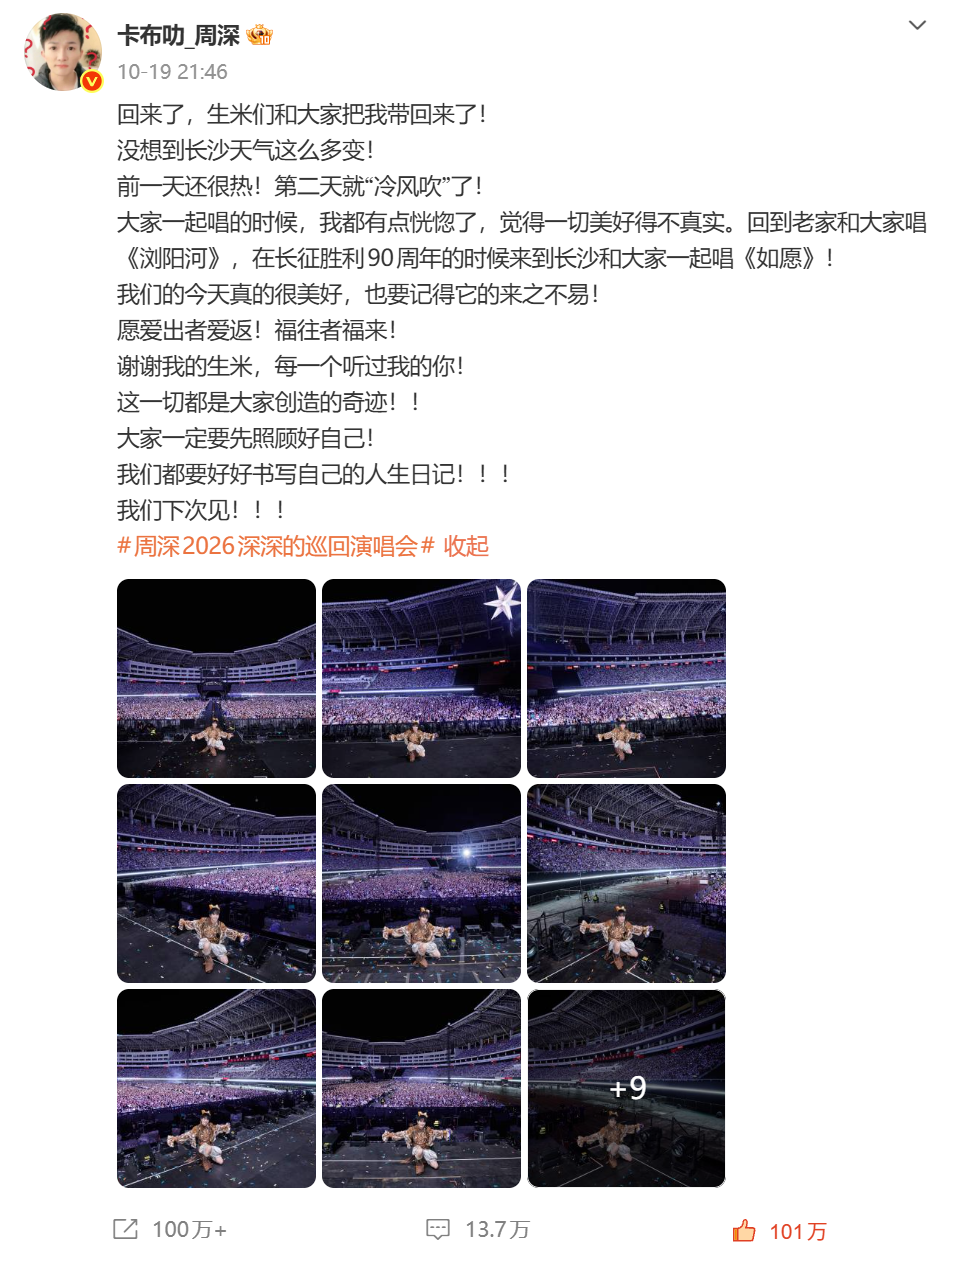
\includegraphics[width=280pt]{img/weibo/ChangSha} 

}

\caption{周深"深深的"巡演2026.10.18长沙场告别微博}\label{fig:unnamed-chunk-56}
\end{figure}

\newpage

\section{整理备注（待人工校对，终稿时删除）}\label{ux6574ux7406ux5907ux6ce8ux5f85ux4ebaux5de5ux6821ux5bf9ux7ec8ux7a3fux65f6ux5220ux9664-7}

\begin{enumerate}
\def\labelenumi{\arabic{enumi}.}
\tightlist
\item
  \textbf{录音来源}：025\_2026深深的\_长沙1018\_内场\_合声版.mp3（约194分50秒，内场合声版）。整理方法：按流程 SOP 全场分段多模态转写（39段×5分钟），唱词对照《appendixG-2026歌词.Rmd》校正，口号互动逐轮记录，低置信处标〔听写待核〕。
\item
  \textbf{本场定位}：2026年''深深的''巡演第25场（长沙 Day2、城市末场，贺龙体育场）；气温骤降场（口播''昨天这么热，今天这么冷的''\,``好冷啊今天''，多次提醒加衣服）；本场吃湖南辣椒环节（``你们说我敢吃这个辣椒不''``刚才那个辣椒，巨辣！''``祝大家红红火火''）；卷首语取自尾声''谢谢你们，因为喜欢听我唱歌，把我带到了体育场开演唱会！我们做到了！``。湖南/长沙元素：长沙话''好不咯''\,``韵味咯''``哦该咯''``嬲噻''、达拉崩吧（湖南卫视《歌手·当打之年》梗）、``长沙的宝哥妹陀''、小城故事改词''长沙故事多/若是你到长沙来/你们的墙头真的多/长沙来做客''、浏阳河引子（昨场次回味）。本场为长沙城市末场，正文末尾已按体例加入城市告别微博截图 R 块（img/weibo/ChangSha.png，截图素材由人工保存提供）。
\item
  \textbf{关键时间点（按5分钟分段定位，录音全长约194分50秒）}：开场VCR 00:00；修星星的人 约02:39（观众先声合唱首句；``长沙的朋友们你们好吗''约04:17）；Try Everything 约07:55；问候+``第二场/降温加衣/长沙话'' 约10:30--13:10；光亮 约12:45（戏曲段约16:10）；若梦 约18:55（合唱逐轮至约22:10）；``人生恍惚三万天''旁白+浮光 约22:20--27:00；借过一下 约27:30（``我找到你们啦''约29:35）；机器人VCR 约31:20；请我不改+警报 约34:35--39:30；来啊（I人尖叫口播） 约40:00--47:30；达拉崩吧 约47:40（``哦该咯''教学约49:20；全名问答约52:15）；反深代词口播+荧光棒 约53:30；蜃楼VCR+天堂岛之歌 约56:30（``有人在看着你''VCR）；记忆商店（鞋掉了互动、冷笑话） 约58:10--61:30；梦见你 约61:45（气球互动约63:50）；荒城渡 约65:00；人是\_ 约67:20（独白约69:50）；音乐动画VCR 约71:30--74:30；化身孤岛的鲸 约73:10（墙头梗约76:40--77:40）；花开忘忧 约78:00；浏阳河引子+《如愿》导语 约82:20；如愿 约83:40（``记住来时路''口播约85:30）；小美满 约87:00（许愿约89:20）；总有美好在路上 约91:30；灯火里的中国 约92:30（``再听一次''多轮）；摄影师魔术（扑克牌） 约96:40--99:10；独上西楼 约99:30（墙头现挂）；小城故事 约100:15；路边的野花不要采 约101:45；我只在乎你 约103:20；面具VCR 约105:00；和光同尘 约106:20（``9.29Hz''应答）；云裳羽衣曲 约107:50；怜悯 约109:20--110:00；望 约110:00；璀璨冒险人 约111:00；奇迹时刻+魔术（铆钉木板、骰子） 约113:50--117:40；好运来+吃辣椒 约117:00--120:40；接财运 约120:50；吉量+想见到气血满满的你 约122:10--126:00（``提问你是谁''互动）；Wala li longla 约126:10（逐词递进多轮）；少管我 约130:00（``优秀真的优秀''口播约132:00）；点歌丢丢（宁波、《玫瑰与小鹿》对唱） 约133:20；耀眼的我们 约137:30；点歌阿雪（广州东北人、《身骑白马》未遂） 约141:10；再一次见面 约145:30；周可可/周嫑嫑 约148:30；致谢 约150:00（``汇风天润/汇丰天润''两读、必应、金少刚Polo衫、安栋小西装、乐尔/悦耳两读、``倒闭''应答）；我以渺小爱你 约154:00；交换日记VCR 约158:40；起风了 约159:50（主歌段欠完整）；大鱼 约163:30；尾声口播（辣椒、愿爱出者爱返） 约166:50；大梦归 约169:20（副歌''吹不灭/不后退/酒一杯''应和版多轮）；告别至录音结束 约173:00（工作人员''开网''调度声约174:30）。〔时间点为分段估算，建议人工复核〕
\item
  \textbf{点歌观众}：第一位丢丢（浙江宁波，第一次来长沙''就是为了来看你''；第一首2019年《玫瑰与小鹿》------周深首支个人原创，与周深对唱''穿过遥远小溪水/守着一株小玫瑰''；与四位歌迷朋友同来；长沙美食蒜香排骨/小龙虾/臭豆腐；感言''遇见你之前我不知道我的生活可以这么的幸福\ldots\ldots 我真的好爱你''，周深''能够鼓足勇气在那么多人面前表达，非常需要勇气''；点《耀眼的我们》并和朋友合照）。第二位阿雪（广州工作的黑龙江东北人，工作七年；``为了你第一次来''长沙；第一首《身骑白马》（蒙面唱将舞台），对唱未遂（``不行不行不行''，周深笑场）；一个人来；点《再一次见面》；``我是在广州的东北人''``我会（粤语）------你好''粤语玩笑）。
\item
  \textbf{VCR 差异}：开场、机器人、面具、交换日记四段 VCR 与《appendixD-2026VCR文字版.Rmd》一致；面具 VCR 开篇日期行本场为''2026年10月18日，长沙''；机器人 VCR 日期句听作''二二二五年五月十七日/第两百天/七万三千天''（与前场''2025年''两读，数字待核）。蜃楼 VCR（天堂岛之歌前）本场为''有人在看着你，有人在看着你，有人在看着你。``（附录D未收录，建议补录）。音乐动画 VCR 纯音乐无词。
\item
  \textbf{长沙场结构差异}（与歌单锚点一致）：Part3 城市限定《如愿》在《花开忘忧》后、《小美满》前（本曲为周深口播''不是我的歌''，含''记住来时路''致敬先辈导语，先以《浏阳河》引子回味昨场）；点歌两首为《耀眼的我们》《再一次见面》；尾曲《大梦归》含观众应和版副歌（``吹不灭''``不后退''``酒一杯''）多轮；本场为城市末场，正文末尾已加微博截图 R 块。
\item
  \textbf{团队名单}（与常州终版一致）：制作必应（1017场听作''比漾''，两读待核）、总导演周佑洋/庄惟惞、音响总监金少刚、音乐总监安栋、乐尔工作室（调音，本场听作''悦耳''）、南京奥斯泰（音响工程）、北京立超舞台集团（硬体）、时代立方（出品）、汇丰天润/汇风天润（承办，两读待核）、周深工作室（出品）、劳伦斯许工作室/Third Studio/Windowsen（服装）、SDT ShowPro（舞蹈）、大麦（票务总代理）、猫眼/票星球（票务代理，``倒闭''应答）。本场致谢：长沙公安/消防/文化等职能部门、场地方长沙城发文旅集团、长沙这座城市；金少刚''天气冷穿外套''关怀梗。
\item
  \textbf{听写存疑}：修星星的人首句与''让我完整''等现场唱词；``演演演演演唱会''口播结巴记法；``深圳的巡回演唱会''（应为''深深的''，口误待核）；请我不改/警报现场演唱版（``摩擦声警报声''``回声却没办法认领''等与附录G差异大）；来啊''Me''应答；达拉崩吧长沙场人名接龙应答（斑得贝迪/哎呦喂/莫得法/啊呜）与''哎呦喂''\,``莫得法''写法；``你们是最好的芒果\ldots\ldots 啊，长沙------噻''口播；蜃楼VCR文字；记忆商店互动小剧（``鞋掉了''``冷笑话''段，冷笑话内容''鬼来到了湖南\ldots\ldots 周嫑嫑''待核）；荒城渡现场版唱词；人是\_副歌合唱欠清晰；浮光后半现场版；小美满现场版首段；``今天就是自己最好的陪伴''合唱改词；总有美好在路上现场版；``灯火荡漾着心中的歌''后口播〔听写待核〕；摄影师魔术段口播；小城故事''唱过一支歌''应答；怜悯应和句；璀璨冒险人''要真的爱要不麻木要有锋芒''现场版；Wala li longla 现场版唱词（夜光的沙/花火玛格丽塔/连梦和云/快乐别调料先邮寄玩耍等）；少管我现场版（造反宇宙/缤纷聚焦/监牢等）；耀眼的我们现场版多处；阿雪《身骑白马》对唱中断段；起风了主歌欠完整；大梦归前段主歌与应和版副歌；致谢''汇风天润''\,``悦耳工作室''两读；若干口播（``你先站住''``点一个菜单啵''等）。
\item
  \textbf{唱词校正说明}：正文唱词均按《appendixG-2026歌词.Rmd》校正，主要修正同1017场外，另含：如愿全段（按附录G）；耀眼的我们（孤独是不是唯一的天赋/踮起脚尖/答案在瞬间清晰/最优的解/验算万万千千/经纬线的距离等）；再一次见面（没反悔之前/习惯回避你视线）；我以渺小爱你（和人生/大雨落山川/三亿岁的石头/相爱支撑命才成为生/灯塔的歌声）；大梦归（春尽枝头慌/岁月漫过熙攘/檐下尽藏/送一袖清晖/果上追/大梦终不归）；璀璨冒险人（炙热/不枉/勇往/呼唤了/多少次传唱/多少伤痕才算活过/愿你哭过）。
\item
  \textbf{待补充}：歌单图（img/playlists/ChangSha-20261018.png）、城市告别微博截图（img/weibo/ChangSha.png）及现场图片待插入。
\end{enumerate}

\chapter{2026.11.07常州场}\label{ChangZhou-20261107}

\begin{quote}
不好意思没能为你们遮风挡雨，但是谢谢你们陪我经历了一切。------周深
\end{quote}

\begin{figure}

{\centering 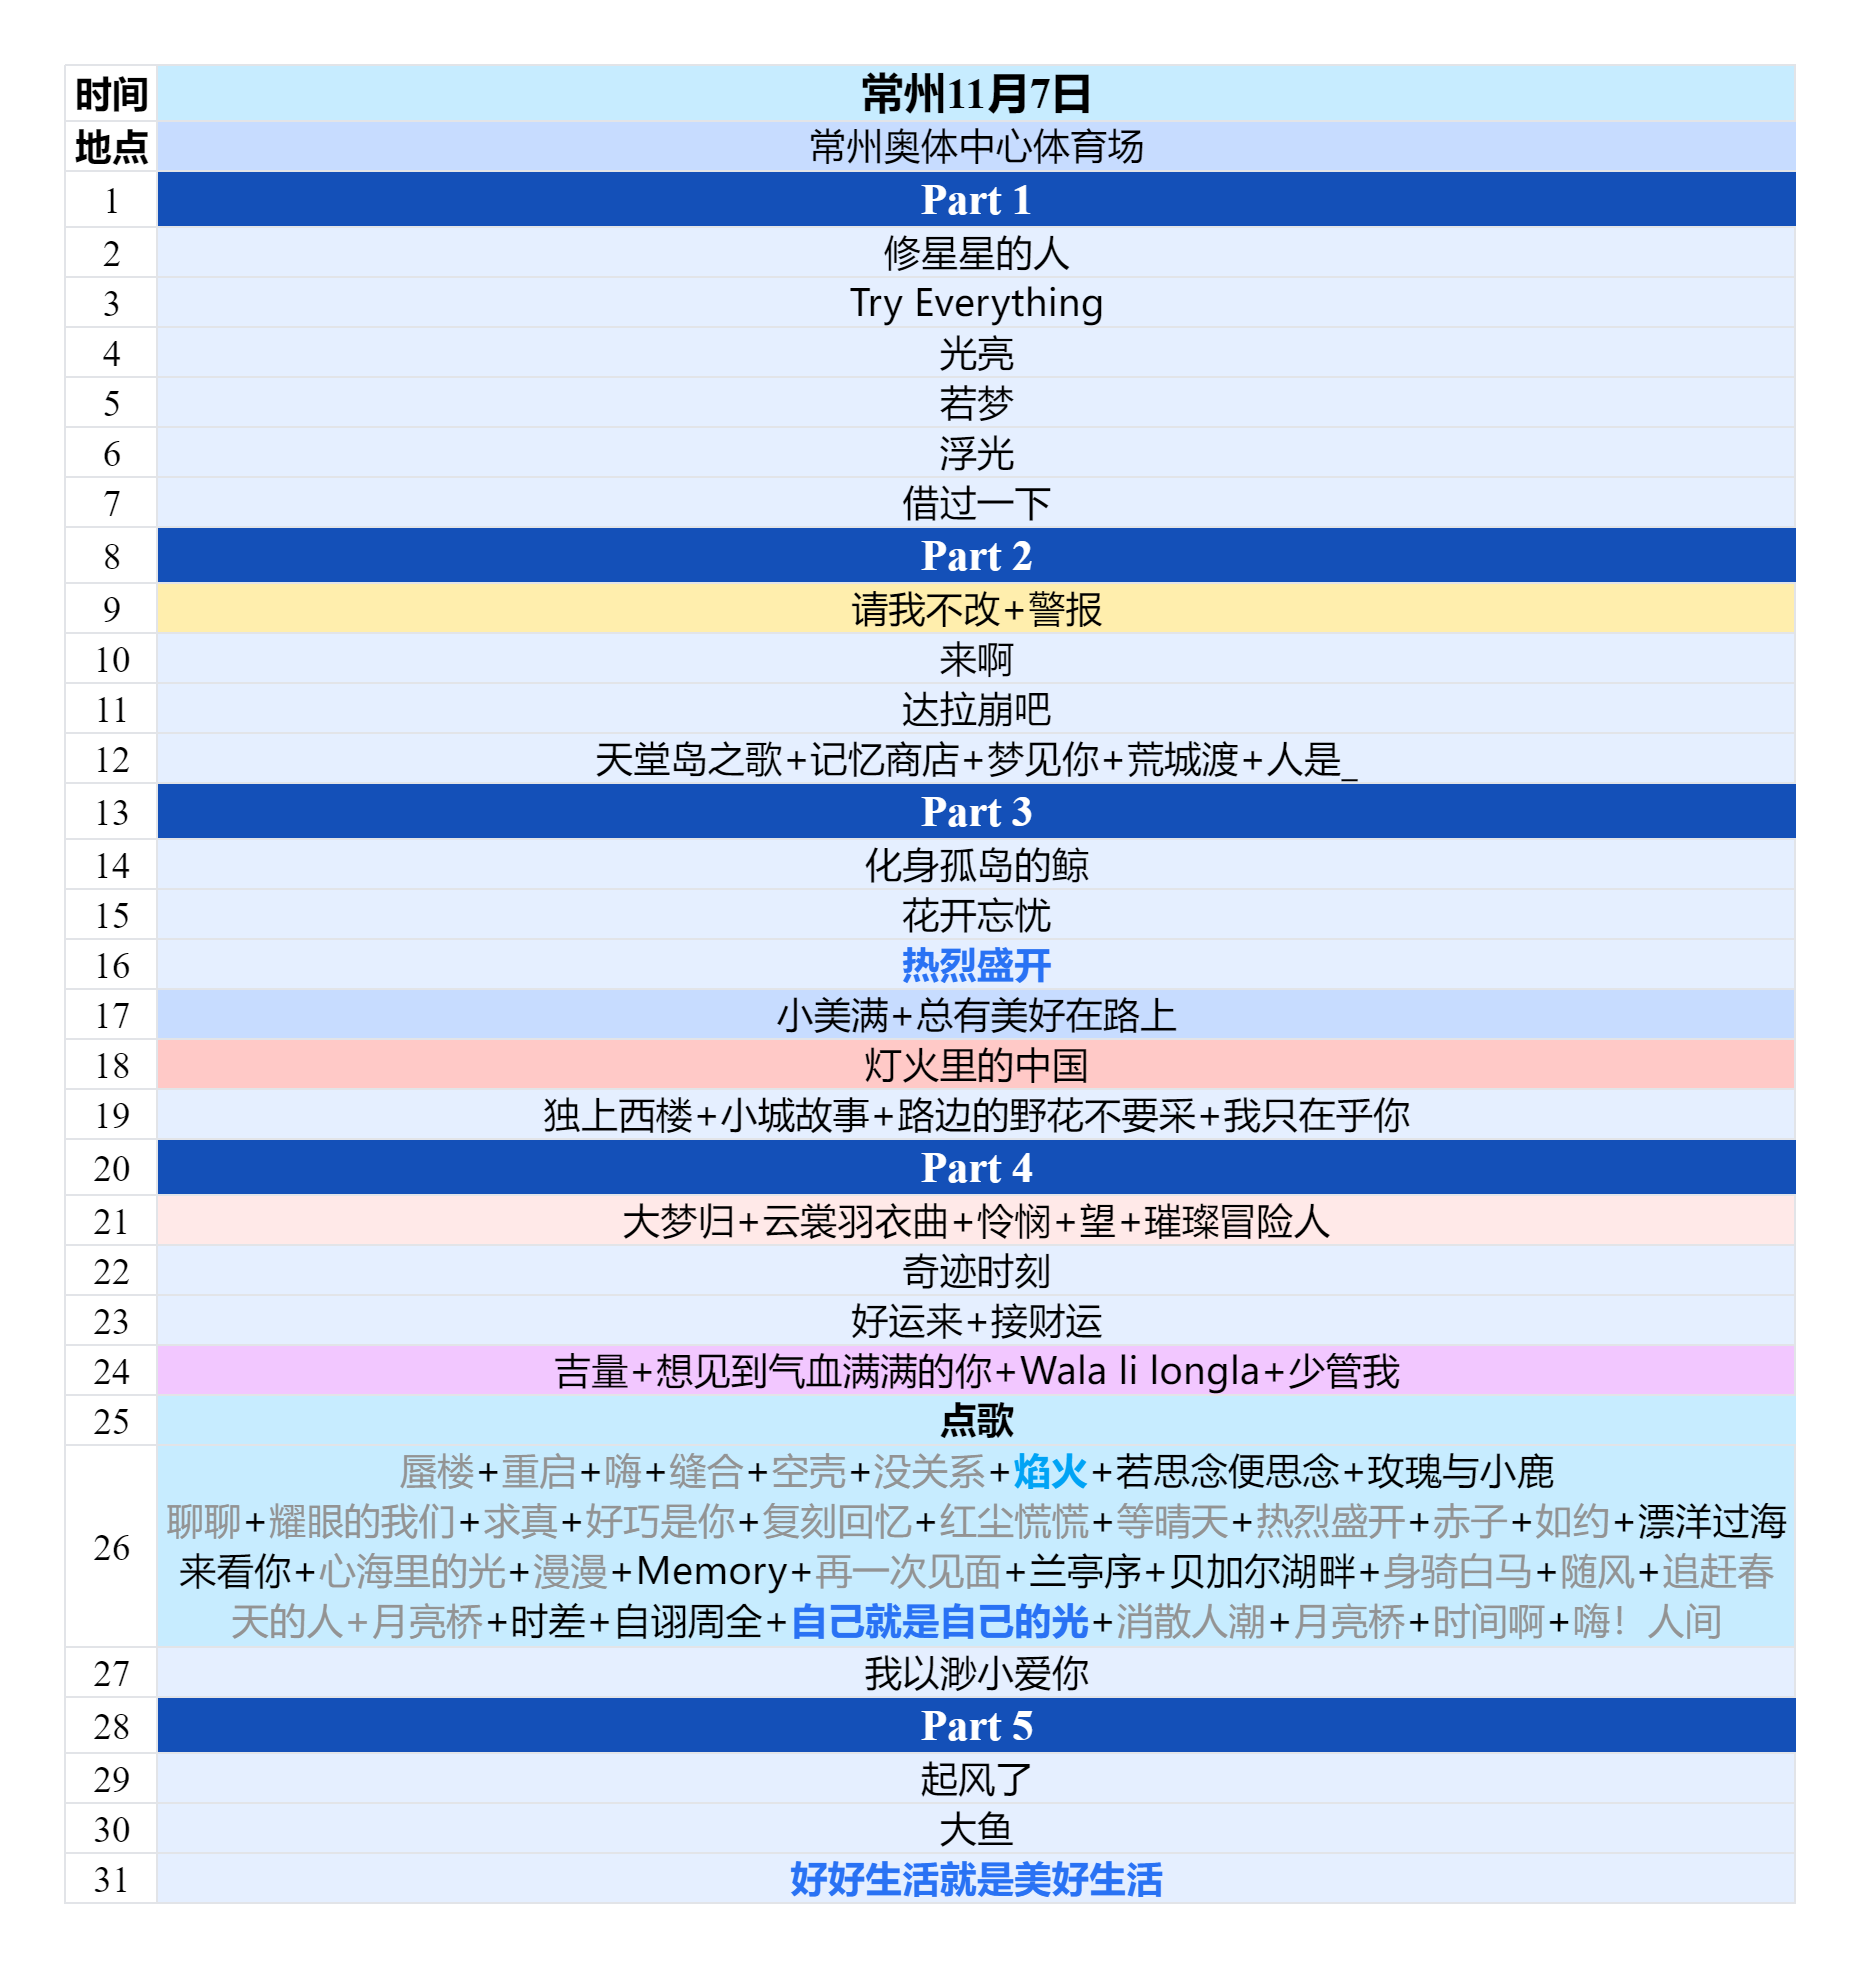
\includegraphics[width=280pt]{img/playlists/ChangZhou-20261107} 

}

\caption{2026周深“深深的”巡回演唱会2026.11.07常州场歌单}\label{fig:unnamed-chunk-58}
\end{figure}

\newpage

\section{Part1}\label{ChangZhou-20261107-part1}

\hyperref[opening-vcr]{🎥【\textbf{开场VCR}】}

\hyperref[xiu-xing-xing-de-ren]{🎵【\textbf{修星星的人}】}（深：在时间的深海里，给常州道一声晚安）。常州的朋友们，你们好吗？（米：好）尖叫声！（米：啊）

\hyperref[try-everything]{🎵【\textbf{Try Everything}】}常州的朋友们，你们好吗？（米：好！）既然宇宙让我们诞生，那就勇敢的Try Everything好不好？（米：好！）尖叫声！常州的朋友，到你们唱！（米：Try everything）再大声！（米：Try everything）最大声！（米：Try everything）。

  哇，我们终于又在深深的巡回演唱会见面了，你们好吗？（米：好）后面的朋友你们好吗？（米：好）这边的朋友你们好吗？（米：好）这边的朋友呢？（米：好）我感觉好久没有见到你们了，让我再听一下你们的声音，常州的朋友你们好吗？（米：好）谢谢大家来到深深的巡回演唱会，谢谢你们把我的人生日记变得这么精彩，谢谢你们让我成为了歌手周深，谢谢大家！大家今天有没有好好的添加衣服呀？（米：有！）有没有穿秋衣秋裤？（米：没有！）没有啊？我作为一个在舞台上要尽量保持形象好点的人，我都穿了秋裤了。一定要注意看天气的变化好不好？（米：好！）来到我们常州，要挑战一下常州话，给我点鼓励。（观众：加油！）【常州话环节】常州的朋友们，大家好，我是周深，总算到常州了。嗯，大家好啊。接下来的不会啦，但是大家欢迎我吗？（米：欢迎）大家也要在常州玩的开心好不好？（米：好！）谢谢你们的出现，让这一切发生。谢谢你们愿意在我任何时刻陪伴着我，也一定要记得，你们需要力量的时候，周深就一直在那里好不好？（米：好！）谢谢你们愿意成为我的光亮。

\hyperref[silver-linings]{🎵【\textbf{光亮}】}到你们（深：可是啊，我却，米：却愿意相信）后面的朋友，（米：最渺小最微弱最柔软最无畏的你，深：用尽了全力）。（深：光亮你自己，我爱你）。（深：六百年一粟，沧海一梦）让我听到你们的声音！（米：合唱）

\hyperref[like-a-dream]{🎵【\textbf{若梦}】}跟你们相遇这件事情，美好的跟做一场梦一样。大声的跟我一起唱若梦好不好？（米：好！）\ldots\ldots 到你们！（米：往事流转在你眼眸）好好听！再来！（米：一边遗忘一边拼凑）（深：如果虔诚，\ldots 唯愿你能得到拯救）谢谢你们的出现，（米：谢谢周深）是谢谢你们。\ldots\ldots 全场！（深：往事流转）（米：往事流转，在你眼眸）后面的朋友！（深：一边遗忘，一边拼凑）（米：一边遗忘，一边拼凑）（深：如我虔诚，合十双手）（米：如我虔诚，合十双手）（深：唯愿你能，得到拯救）全场最大声！（米：往事流转，在你眼眸，深：在你眼眸）（米：一边遗忘，一边拼凑，深：一边拼凑）（米：如我虔诚，合十双手，深：合十双手）（深、米：唯愿你能，得到拯救）到你们！（米：唯愿你能，得到拯救）（深：因为\ldots\ldots 你你你你你你\ldots\ldots 你们，周深才得到拯救------）。

\hyperref[floating-light]{🎵【\textbf{浮光}】}人生恍惚三万天，因为遇见了你，每一天都特别特别的有意义，谢谢你，出现在这个人世间，你真的很好，要记得，好不好？（米：好）\ldots\ldots 到你们！（米：浮光掠影重山彩云间）大声唱！（米：你的伏线穿越千百年）再大声！（米：人生不过恍惚三万天，漫漫人间，留恋流连）。

\hyperref[excuse-me]{🎵【\textbf{借过一下}】}谢谢你，给我力量，让我说出这一句，借过一下。（深：少年扬起脸庞，前往他的月亮\ldots\ldots 你们都是对的，他说拜托，让开一下）。（深：潇洒不是不怕，是愿付出代价）你还愿意吗？（米：愿意！）。（深：谢过赐教的话，路借过一下）尖叫声！（米：啊啊啊）全场！（深：让我大醉一场，米：殿堂之上，背闲诗两三章）再大声（深：让我穿白衣裳，米：过疯人巷，去泥潭捞月光；深：望大人们见谅，提点的话，我懂也不想装，世人寻黄金乡，我找月亮，何必同往）。到你们（米：话谢过，路借过，你是你，我是我）最大声（米：话谢过，路借过，你是你，我是我）\textbf{\textcolor{red}{我爱你们}}！（深：人见过明暗 若天真犹在，当披上月光，走夜晚）你们就是我要找的月光，我找到你们了！（米：啊啊啊）

\section{Part2}\label{ChangZhou-20261107-part2}

\hyperref[robot-vcr]{🎥【\textbf{机器人VCR}】}

\hyperref[brave-heart]{🎵【\textbf{请我不改}】}常州的朋友们！（米：啊啊）你们好吗？（米：好）（深：\ldots\ldots 才看清追兵与逃兵，竟都是我自己）尖叫声！（深：请我不改，我的姿态，我的爱我的痛都与生俱来\ldots\ldots 放肆盛开）（深：Brave heart）到你们！（米：Brave heart！）尖叫声！（深：Brave heart）到你们！（米：Brave heart！）（深：Brave heart）到你们！（米：Brave heart！）
\hyperref[jing-bao]{🎵【\textbf{警报}】}（深：我发送警报声，血红色惊叹号，提醒你自救。被遥控，被耗空，快失控，快断送\ldots\ldots 从借用到利用到滥用，转身就走\ldots\ldots）。

  接下来这首歌，想要你们跟我一起唱，这首歌叫《来啊》，肯定有很多人没有听过，那我们可以现场就立马学会。没错，谁说的周深的歌很难学？试一下啊。我喊''Don't tell me''，你们就------来！（米：来）好不好？（米：好）（深：Don't tell me）（米：Lie eeeeee lie eeeeee）哦，后面的朋友跟我们一起唱哦。（深：Don't tell me）（米：Lie eeeeee lie eeeeee）再大声点。（深：Don't tell me）（米：Lie eeeeee lie eeeeee）大家要不要来常州玩？（米：要！）所以就------来！（米：Lie eeeeee lie eeeeee）哦，好不整齐哦。

\hyperref[lai-a]{🎵【\textbf{来啊}】}全场！（深：Don't tell me）（米：Lie eeeeee lie eeeeee）（深：我望眼欲穿你别闪躲）再来（深：Don't tell me）（米：Lie eeeeee lie eeeeee）。再来。（深：随你操控）\textbf{\textcolor{red}{我爱你们}}！再来（深：Don't tell me）（米：Lie eeeeee lie eeeeee）（深：我望眼欲穿你别闪躲\ldots\ldots 敢不敢直视我，Let's fall）

  谢谢你们！（米：谢谢周深！）啊不不不，是谢谢大家。那接下来到了我们深深的巡回演唱会小游戏环节啦。每个人呢可以自行变换你喜欢的颜色，我们的荧光棒可以自己换颜色哟。好像也不是很厉害的事情哈。分别是红色、蓝色\ldots\ldots 粉红色、蓝色、黄色和绿色。不同的颜色代表着不同的角色。但是无论选择什么样的颜色，你们都是人生当中最美的------（米：角色！）没错哦。快选吧，给你们五秒钟的时间。五、四\ldots\ldots 选择不同的颜色都有不同的角色，他们分别是蓝色代表的是达拉崩吧，黄色代表的是国王陛下，粉红色代表的是公主米娅，那绿色代表的是------（米：恶龙！）我们这条龙终于来到了常州。（米：哇！）大家要记得去玩哦。（米：好！）常州恐龙\ldots\ldots 选择不同的角色有他们相对应的台词，所以当我喊出你们的名字的时候，要大声喊出他的台词好不好？（米：好！）来咯。达拉崩吧！（米：我最棒！）国王陛下！（米：再说一次！）公主米娅！（米：救我啊！）恶龙！（米：啊呜！啊呜！）那有很多红色的朋友，我相信应该是我刚才说错了，所以你们选错了对不对？那我们红色的朋友都统一按照公主米娅来处理吧。公主米娅！（米：救我啊！宝贝）诶。那红色的朋友如果我们喊常州------（米：宝贝！）我就知道会是这样，所以我甚至这一次连我们红色的对暗号那个暗号我都没有学习。常州！（米：宝贝！）哎，配合一下嘛。我喊常州你们喊''土豪''好不好？常州！（米：宝贝！）是我听错了吗？常州！（米：宝贝！）摘了耳机听得更清楚了。达拉崩吧！（米：我最棒！）国王陛下！（米：再说一次！）公主米娅！（米：救我啊！）恶龙！（米：啊呜！啊呜！）恶龙！（米：啊呜！啊呜！）达拉崩吧！（米：我最棒！）国王陛下！（米：再说一次！）公主米娅！（米：救我啊！）恶龙！（米：啊呜！啊呜！）常州！（米：宝贝！）常州！（米：宝贝！）恶龙乘以十，走！（米：啊呜！啊呜！啊呜！啊呜！啊呜！啊呜！啊呜！啊呜！啊呜！啊呜！）你们真的很愿意配合我一起喊口号。那，常州！（米：宝贝！）我们一起来重温一下《达拉崩吧》这个童话故事吧。

\hyperref[dalabengba]{🎵【\textbf{达拉崩吧}】}荧光棒！（深：很久很久以前，巨龙突然出现，带来灾难，带走了公主又消失不见\ldots\ldots 他说，陛下我叫，达拉崩吧斑得贝迪卜多比鲁翁，再说一次，达拉崩吧斑得贝迪卜多比鲁翁）全场，达拉崩吧！（米：我最棒！）国王陛下！（米：再说一次！）公主米娅！（米：救我啊！）恶龙！（米：啊呜！）恶龙！（米：啊呜！）常州！（米：宝贝！）达拉崩吧！（米：我最棒！）你可真是太棒了！（深：英雄达拉崩吧，骑上最快的马，带着大家的希望，从城堡里出发\ldots\ldots 巨龙说，我是昆图库塔卡提考特苏瓦西拉松，再来一次，昆图库塔卡提考特苏瓦西拉松，是不是，昆特牌提琴烤蛋挞苏打马拉松，不对是，昆图库塔卡提考特苏瓦西拉松）达拉崩吧！（米：我最棒！）国王陛下！（米：再说一次！）公主米娅！（米：救我啊！）恶龙！（米：啊呜！啊呜！）达拉崩吧！（米：我最棒！）国王陛下！（米：再说一次！）常州！（米：宝贝！）（深：于是，达拉崩吧斑得贝迪卜多比鲁翁，砍向，米：昆图库塔卡提考特苏瓦西拉松）后面的朋友！（深：然后，米：昆图库塔卡提考特苏瓦西拉松）咬了！（米：达拉崩吧斑得贝迪卜多比鲁翁。深：最后，达拉崩吧斑得贝迪卜多比鲁翁，战胜了，昆图库塔卡提考特苏瓦西拉松）再大声！（深：救出了，公主米娅莫拉苏娜丹妮谢莉红）后面的朋友！（深：回到了，蒙达鲁克硫斯伯古比奇巴勒城\ldots\ldots 就把，公主米娅莫拉苏娜丹妮谢莉红，嫁给了，达拉崩吧斑得贝迪卜多比鲁翁\ldots\ldots 他们生下一个孩子，也在天天渐渐长大，为了避免以后麻烦，孩子称作王浩然）他的全名是------（米：达拉崩吧斑得贝迪卜多比鲁翁！）这位大哥一个字都不帮我念吗？达拉？好高冷。那他的口号是达拉崩吧！（米：我最棒！）国王陛下！（米：再说一次！）公主米娅！（米：救我啊！）常州！（米：宝贝！）常州！（米：宝贝！）公主米娅！（米：救我啊！）再这样我要让你们喊十遍达拉崩吧的全名了。恶龙乘以十，走！（米：啊呜！啊呜！啊呜！啊呜！啊呜！啊呜！啊呜！啊呜！啊呜！啊呜！））哦？怎么来念？（深：要念你来念吧）尖叫声！（米：啊啊啊）。

  大家有吃萝卜丝炒饭吗？（观众：没有！没吃到！）哦有很多人没有吃是吗？一定要去吃，真的很好吃。我第一次来到常州吃到那个萝卜丝炒饭，我第一反应就看这个名字。（观众：萝卜干！）萝卜干炒饭。萝卜干炒\ldots\ldots 切成了萝卜丝炒的饭。萝卜干炒饭，我第一次吃到萝卜干炒饭，说实话第一次看名字，萝卜干炒饭能有多好吃？然后吃完就\ldots\ldots 哇！它为什么只是叫萝卜干炒饭？大家一定不要错过好不好？（米：好！）常州还有非常非常多好吃的东西。在前年我发了一张专辑叫做------（米：反深代词！）谢谢。叫《反深代词》，很多人肯定还不知道这张专辑。这张专辑呢说的是200年后的世界，有个这个世界叫做反深代词。周深一共化成了12个不同的情绪碎片在那个200年后的反深代词的世界。所以如果你在听这张专辑的时候，你发现某首歌跟你的情绪、跟你故事一模一样的证明，我们在200年后的这个世界彼此相互拥抱安慰了。所以求求大家去听一下这张专辑好不好？（米：好！）后面的朋友你们去听一下这张专辑好不好？（米：好！）在今年，这张专辑还发了它的实体专辑。（米：啊啊啊）应该还有一些朋友还没有收到。希望大家\ldots\ldots 就谢谢大家就是\ldots\ldots 的谅解吧，因为它制作稍微有一点点复杂。希望大家拿到这个专辑的时候也一定要像我一样，因为是遇到了你们，才给我勇气去看见自己那么多面、那么多情绪。也希望你们可以听完这张专辑之后，也可以去好好的看见自己，和保护好自己好不好？（米：好！）那让我们看一下，在反深代词的蜃楼当中，后面又发生了一些什么样的故事吧。

\hyperref[haven-song]{🎵【\textbf{天堂岛之歌}】}（一个两个三个小朋友\ldots\ldots）（深：叮咚，我有一个秘密，悄悄告诉你，欢迎你来到天堂入口\ldots\ldots 叮咚有人在看你的过去）生米们，你们在哪儿？（米：在这儿！）听过周深唱歌的你，在哪里？（米：在这里！）
\hyperref[the-memory-store]{🎵【\textbf{记忆商店}】}（BGM）诶？这是深深的巡回演唱会吗？（米：是！）这是秋衣。我上一次梦见这个场景的时候还没有穿秋衣啊。这是秋裤。这是深深的巡回演唱会吗？（米：是！）达拉崩吧！（米：我最棒！）常州！（米：宝贝！）还是那一群不愿意配合我说口号的朋友。哦，我知道了，这是《反深代词》那个世界当中的记忆商店。你们为什么没有穿秋衣？哦，只要拥有这一颗米子心，我们就可以唤醒我们最喜欢的那一段回忆。但是跟你们相遇的每一分每一秒，都是我最幸福的时刻。那让我们一起来看一下好不好？（米：好！）要好好穿好秋衣秋裤哦。（米：好！）
\hyperref[meng-jian-ni]{🎵【\textbf{梦见你}】}（深：看着眼前，还年少的你，恍如流年从未淌过去\ldots\ldots 与你重逢在另一场梦境，但愿那时你在人海里，仍将我一眼认清）全球震撼首发，我们找到了常州恐龙蛋。你们在做些什么？要如何捏爆它？下一次你会不会就是踩着一个气球出来？就像那个水上游乐\ldots\ldots 游乐项目。你有给它取名字吗？（舞蹈老师：嗯\ldots\ldots 常州！）（米：宝贝！）那就让我们来看一下这个常州恐龙蛋存放着什么样的记忆吧。哇雷声大雨点小哎。效果好差，灭掉。
\hyperref[huang-cheng-du]{🎵【\textbf{荒城渡}】}（深：夜色中寻觅过，当往事困住我，也盼心中生出一点萤火\ldots\ldots 断了这心魔，可原谅我，宿命中获得这解脱，重来过。眼中拂尘，手中残魂，那故事斑驳荒城\ldots\ldots 握一颗糖暖这孤身颠簸）。
\hyperref[Humans_are_]{🎵【\textbf{人是\_}】}（深：未知摊开棋局，舍弃昨日才可破，再见了我的月光，\ldots\ldots 让死亡觊觎我，让恐惧亲吻我，来摧毁我深爱的一切，可仍夺不走我的选择）。你们帮我！（深：让时空消亡我）唱！（米：你无需记得我）。再来（深：弹指间湮灭我）（深：弹指间湮灭我，米：但命运打不败活着）（深：是微茫中高歌的族类，生命像烟火那就点亮，孩童的双眸）到你们，（米：未来的瞳孔，深：未来的瞳孔）。

  在遇到你们之前，我也认为那些失去的过去的才是最美好的。但是因为听到了你们的大声歌唱，让我明白我们现在相遇的每一分每一秒，我们现在拥有的一切才是最珍贵的宝藏。你们说，对吗？（米：对！）【BGM：不朽的永恒的，我们记得，不朽的永恒的，我们记得】是你们创造了不朽的永恒的爱。\textbf{\textcolor{red}{我爱你们}}！

\section{Part3}\label{ChangZhou-20261107-part3}

\hyperref[music-animations-vcr]{🎥【\textbf{音乐动画VCR}】}

\hyperref[The-whale-who-became-an-island]{🎵【\textbf{化身孤岛的鲸}】}常州的朋友们你们好吗？（米：好！）（深：我是只化身孤岛的蓝鲸，有着最巨大的身影\ldots\ldots 你的衣衫破旧，而歌声却温柔）。谢谢你们的出现。（米：谢谢周深）。（深：鱼虾在身侧穿行，千万不要不穿秋衣）。你们来！（深：你的衣衫破旧，米：而歌声却温柔，陪我漫无目的的四处漂流）（深：我的背脊如荒丘\ldots\ldots 我想给你能奔跑的岸头）（米：没有墙头！）常州的朋友！（米：没有墙头！）（深：你们有多少个墙头？）（米：没有！）很多我们常州的朋友，你们不知道，啊？墙头什么意思啊？周深在干什么？好奇怪。哦，就是当我问我的生米们，我说你们喜欢哪个歌手唱歌，他们会说\ldots\ldots（观众：周深！）哎，那我又非常之不知足很讨厌的又要问啊，你们除了我还喜欢哪些歌手啊？（观众：没有！）他们就会骗我说没有。但其实他们有很多其他喜欢的歌手。我就非常非常非常的没有礼貌的，把其他的歌手老师们称为''墙头''。所以我会问，（深：你们到底有多少个墙）\ldots\ldots 然后带点哭腔，头\ldots\ldots（观众：没有！）但是无论怎么样，好好照顾好你自己，因为你是我的国王和王后。〕

\hyperref[Blossoms-that-forget-sorrow]{🎵【\textbf{花开忘忧}】}常州的朋友，你们好！我们来常州看你咯！（米：欢呼）你有没有好好照顾好自己啊？（米：有！）一定要做到好不好？（米：好！）（深：巷子口买了花，穿过沿街红墙青瓦\ldots\ldots 一件遗憾的事就喝一碗汤，庭院深深，秋叶飘落）（深：若记忆被偷走了，忘了我的爱，我会说）说什么？（米：你好啊！）你们好吗？（米：好！）（深：这是给你的花，花的名字叫忘忧草，它说时光汹涌如水上烟波，别走远了一起回家）我们一起回家好不好？（米：好！）谢谢你的到来，谢谢你的出现。\textbf{\textcolor{red}{我爱你们}}！（米：我也爱你！）一起！（深：我们苍老的时候就回到小时候，采青梅用来酿酒你不许偷着喝，穿朴素的衣裳牵着那衣袖，捡了小猫名为苍狗）到你们！（米：我们睡去的时候像孩子无忧愁，反正也很难上锁这岁月如小偷，若记忆被偷走了忘了我的爱）。（深：忘忧草开着花，你在月光下不说话，一件遗憾的事就喝一杯茶，庭院深深，秋叶飘落）。

  在我们的人生当中，一定有那么一个人，非常非常重要。也住着这样一份遗憾，再也没有机会见到他。但是我相信，只要我们的思念喊得越大声，他一定听得到，对不对？（米：对！）所以我们一定要好好照顾好自己，因为他们也一定感受得到。你们说对吗？（米：对！）花开忘忧，愿你无忧！（米：花开忘忧，愿你无忧。）花开忘忧！（米：愿你无忧！）好好照顾好自己好不好？（米：好！）你们好吗？（米：好！）后面的朋友你们好吗？（米：好！）

  没有想到，我跟我们常州非常有缘分。有一首歌跟常州非常非常有关系。这首歌的首唱也是在这个体育场唱的。（米：啊啊）你们听过吗？（米：听过！）这首歌叫？（米：热烈盛开！）你看我们常州多厉害。在上一届苏超，它获得的名次是？声音很小声。倒数第二名。诶，但是你看，《热烈盛开》就厉害在这里。今年我们常州获得的名次是？所以呀，我们就要不停的努力，好好的去成为自己。每一个努力每一次奋斗都是有用的对不对？（米：对！）我们一起去面对我们的热烈盛开，我们也一定会热烈盛开对不对？（米：对！）那等一下大家跟我一起唱。好不好？（米：好！）我们也祝我们常州越来越好，三二一，祝常州------（米：越来越好！）

\hyperref[re-lie-sheng-kai]{🎵【\textbf{热烈盛开}】}跟我一起（深、米：我会热烈的热切的盛开，开在荒野开在小小角落与人海，山有其巍峨我有我姿态，向阳而生会有风为我而来。我要绚烂的骄傲的盛开，开在山巅开在雪花飘落的窗台，我当奔赴我的热爱，邀万里长风为我喝彩）好好的去写好你的人生日记，好不好？（米：好！）我们一定热烈盛开，对不对？（米：对！）（深：所有的未来都来自现在\ldots\ldots 我的心永不改）全场唱！（深、米：我会热烈的热切的盛开\ldots\ldots）唱！后面的朋友！（深、米：我当奔赴我的热爱，邀万里长风为我喝彩）再大声，一起！（深、米：我会热烈的热切的盛开\ldots\ldots 有万里长风为我喝彩）。

\hyperref[simple-bliss]{🎵【\textbf{小美满}】}那这首歌你会唱吗？（米：会！）大声！（深：没什么大愿望）唱（米：没有什么事要赶\ldots\ldots 乌云还挺大胆，顶在头上吹不散，我抓在手里捏成棉花糖，什么烦恼不能忘）\ldots\ldots 全场一起！（深：你看小狗在叫，树叶会笑，风声在呢喃）。你们真的特别的美好，谢谢你们。（米：谢谢周深。）来！（深：笑一笑就灿烂）怎么了？（米：唱一句歌就舒展）（深：收集一点一滴小美满都是幸福的花样，没道理的开朗）唱！（米：打扮平凡的日常）。\ldots\ldots 大声唱。\ldots\ldots 谢谢你们给我这么这么幸福的小美满，谢谢你们。（米：谢谢周深。）

  让我们一起在小美满这首歌当中许愿吧。像我这样闭上眼睛想好你的愿望，我会倒数三二一，睁开眼睛，我们的愿望就会出现在这棵许愿树上。请相信你们的力量，请相信相信的力量，请相信美好的力量。现在现场每一个朋友闭上眼睛，无论什么年龄段，无论什么职业，闭上眼睛许愿吧。想想你最想要实现的愿望是什么呢？生日的时候第一个蹦出来的愿望是什么呢？哦对了，小美满这首歌当中的愿望只能够许关于你自己的愿望。想一想是不是很久没有拥抱过自己了？是不是很久没有跟自己说一声，你走到现在真的真的很棒，你真的拼尽全力而且做得非常好了？是不是很久没有跟自己说一声，你辛苦了？三二一，睁开眼睛，我们的愿望一定会实现的对不对？（米：对！）（深：笑就好，哭也好，今天就是明天最好的陪伴，笑就好，哭也好，你们都是周深最好的陪伴）到你们！（深：自己，米：就是自己最好的陪伴）因为你们的出现，每一天都非常有意义。

\hyperref[zong-you-mei-hao-zai-lu-shang]{🎵【\textbf{总有美好在路上}】}哦，让我们祝今天生日的朋友！（米：生日快乐！）你们太美好了。让我们祝昨天或者是前一段时间过生日的朋友！（米：生日快乐！）让我们祝明天或者是过一段时间才过生日的朋友！（米：生日快乐！）谢谢你们的美好，谢谢你们的善意，就是因为你的出现才让我看见。（深：花在开，云在飘，笑容在脸上，我们向前方一路向阳）到你们！（深：亲爱的你）（米：在路上慢慢逛，看一看太阳，深：让风轻轻，米：吹拂你的脸庞）后面的朋友。（深：今天过去，米：要到明天看看天气会怎样，深：阴或晴朗，故事都慢慢赏吗，抬头发现，你们就是光芒）。

\hyperref[deng-huo-li-de-zhong-guo]{🎵【\textbf{灯火里的中国}】}灯火里的中国，美不美丽？（米：美！）那也是因为有最美好的你组成的。所以一定要好好好好的看见自己，好吗？（米：好！）（深：都市的街巷已灯影婆娑\ldots\ldots 灯火里的中国青春婀娜，灯火里的中国胸怀辽阔，灯火漫卷的万里山河，初心换回了百年承诺）等下跟我一起大声唱好不好？（米：好！）后面的朋友一起唱好不好？（米：好！）大声唱！（深：灯火里的中国）（米：青春婀娜）（深：灯火里的中国）（米：胸怀辽阔）大声唱！最大声！（深：灯火里的中国，青春婀娜）唱（米：灯火里的中国，胸怀辽阔）。（深：灯火荡漾着心中，米：的歌，深：的歌）。

  你们唱的太好听了。我还想再听一遍你们唱副歌耶。再唱一遍副歌给我听好不好？（米：好！）后面的朋友再唱一遍副歌给我听好不好？（深：灯火里的中国，米：青春婀娜）（深：灯火里的中国，米：胸怀辽阔）（深：灯火漫卷的万里山河）（米：初心换回了百年承诺）再大声。（深：灯火里的中国，米：青春婀娜，深：灯火里的中国，胸怀辽阔）（米：灯火灿烂的中国梦）（深、米：灯火荡漾着心中的歌）。

  恭喜你，接受我们高音挑战。（深：啊啊啊）（摄像老师：啊！）糟糕，他准备好了。他能唱完吗？（深：啊啊啊）没人拍你是吗？我拍你。等一下，这怎么用啊？别摔坏了，我赔不起哦。好，来啊。（深：啊啊啊）你第几次来常州啊？第几次来常州？（摄像老师：第一次。）就留下刚才这样美妙的歌声。（摄像老师：永生难忘。）哦，那\ldots\ldots 我生米们很厉害的。（深：啊啊啊啊啊，米：啊啊啊）谢谢你们。（米：谢谢周深。）

🎵【\textbf{邓丽君组曲}】\\
  谢谢。我很开心成为歌手，因为我从小也是一个非常喜欢听歌的人。那就有这样一个歌手啊，我就想要成为她这样，有好多首歌陪伴大家。就是邓丽君女士。所以如果你听到她的歌，你们会唱对不对？（米：会！）那等下跟我一起大声唱好不好？（米：好！）

\hyperref[du-shang-xi-lou]{🎵【\textbf{独上西楼}】}（深：无言独上西楼）刚才我才发现整个舞台上只有你这一个摄像老师在，他们都跑得好快。（深：月如钩，寂寞梧桐，深院锁清秋，剪不断，理还乱，是你们的墙头）（米：没有！）（深：还在美丽的常州，说你们没有墙头）（米：没有！）
\hyperref[xiao-cheng-gu-shi]{🎵【\textbf{小城故事}】}我们在哪座城市？（米：常州！）跟我一起唱。（深：常州故事多）唱（米：充满喜和乐）（深：若是你到常州来，萝卜干特别多〕）大声唱！（米：看似一幅画）听呢？（米：听像一首歌）（深：人生境界真善美，常州已包括）到你们。（米：谈的谈，说的说）（深：你们墙头真的多）（米：没有！）（深：请你的朋友一起来，来哪里？）（米：常州来做客。）你们来！（米：请你的朋友一起来）后面的朋友来哪里？（米：常州来做客。）
\hyperref[donot-pick-the-roadside-flowers]{🎵【\textbf{路边的野花不要采}】}这首歌会唱吗？（米：会！）让我听到你们声音好不好？（米：好）（深：送你送到小村外，有句话儿要交代。虽然已经是百花开）你们，（深：路边的野花）它怎么啦？（米：不要采！）大声唱出来！（米：记着我的情，记着我的爱，记着有我天天在等待）（深：我在等着你回来。千万不要把我来忘怀，千万不要把我来忘怀，千万不要把我来忘怀）你们会忘了我吗？（米：不会！）
\hyperref[I-only-care-about-you]{🎵【\textbf{我只在乎你}】}谢谢你们。我经常想过很多次，如果不是你的出现，我现在在干什么呢？我真的没有找到那个答案。（深：如果没有遇见你，我将会是在哪里？日子过得怎么样？人生是否要珍惜？）（米：也许认识某一人，过着平凡的日子，不知道会不会\ldots\ldots）（米：宝贝）宝你们个头！（米：啊！宝贝！）（深：任时光匆匆流去，我只在乎你。心甘情愿感染你的气息。人生几何能够得到知己？失去生命的力量也不可惜。）到你们。（米：所以我求求你，别让我离开你。）（深：除了你，我不能感到一丝丝情意。）再大声！（深：任时光匆匆流去，我只在乎你）谢谢你们！再大声！（深：心甘情愿感染你的气息）（深：人生几何）怎么了？（米：能够得到知己？深：失去生命的力量也不可惜。所以我求求你，别让我离开你。除了你，我不能感到一丝丝情意。）到你们。（米：除了你，我不能感到一丝丝情意。）（深：除了你，我不能感到一丝丝情意。）你们会忘了我吗？（米：不会！）我！只！在！乎！你！

\section{Part4}\label{ChangZhou-20261107-part4}

\hyperref[mask-vcr]{🎥【\textbf{面具VCR}】}

（VCR：我相信我们一定能找到属于自己的答案的，你说，对吗？）（米：对！）没听到哦。你说，对吗？（米：对！）

\hyperref[da-meng-gui]{🎵【\textbf{大梦归}】}你们会唱这首歌吗？（米：会！）（深：春尽枝头慌，再一季，花开无人赏，再一句，感人间万般皆寻常\ldots\ldots 檐下尽藏缕缕香）。你们会唱吗？（米：会！）让我听到哟。（深：就让，米：冷风吹，雨纷飞，留一地伤悲，就让爱破碎，恨成灰，往事都作废）（深：就让火一堆，酒一杯，送一袖清晖，就让因后退，果上追，大梦终不归）。
\hyperref[Song-of-the-cloud-dress]{🎵【\textbf{云裳羽衣曲}】}我们的缘分一定不会太浅，因为我的名字叫------（米：周深！）因为我们的巡回演唱会的名字叫------（米：深深的！）我们继续大声歌唱好不好？（米：好！）（深：故事鲜艳，而缘分却太浅）唱！（米：我的爱恋，竟如此的明显）（深：我不停地默念，想牢记你的容颜）再大声！（深：故事鲜艳，而结局却搁浅，这些年你又在那座红尘之间，幻化成哪张脸）。\ldots\ldots 谢谢你们的出现。（观众：谢谢周深。）
\hyperref[lian-min]{🎵【\textbf{怜悯}】}（深：我要比你显得更无情，再生一场病）（米：怜悯是讨来的公平）（深：我要带着爱意恨着你，逢人就美化你罪行。我要抱着余烬守伶仃，蘸着真心，隔岁月惦念你）。\ldots\ldots 我们不要祈求怜悯，我们都值得被好好的爱着，你们说对吗？（米：对！）
\hyperref[Expectation]{🎵【\textbf{望}】}所以无论你在哪儿，我们都会绕啊绕，绕回彼此身边。（深：我们总会绕啊绕，绕啊绕，绕几千里路也望向归途）。\ldots\ldots 一起唱！（深：我们总会，米：绕啊绕，绕啊绕，绕几千里路也望向归途）我们的朋友我看到你了。（深：乘着风，想念吹拂，有夜空漂浮，抓一颗流星做礼物，愿你幸福。手中线，绕啊绕，绕啊绕，绕几千日夜也望向归途，燕归巢，迁徙之路，参与者无数，待到烟火照夜白时准备庆祝，我们心有所住）。
\hyperref[adventurers]{🎵【\textbf{璀璨冒险人}】}璀璨冒险人你准备好了吗？（米：准备好了！）我们一起向前冲吧！（深：他们说要越过前方风沙，必须低着头；他们说要绕过蜿蜒的河，才能往前走；他们说烫要放手，太远要换个路口；如果得不到谁的认同，那就不算拥有）到你们！（深：没人能够决定谁的一生应该怎么活）再来！（深：没人能够定义谁的天空是什么颜色；没人未梦就先懂，只是单纯相信着；背向光的英雄，每张轮廓出自平凡的沉默）你们都是我的英雄，谢谢你们！（米：谢谢周深）。（深：就让一路曲折，每一道伤口，洗净我的脆弱）全场一起！（深：原来咽回去的泪，才能淹没了脆弱。你发誓更勇敢，一生与梦相拥）。（深：\ldots\ldots 要炙热啊！要不忘啊！要勇往啊！起风了，呼唤了，你还在等什么？挥手了，再见了，别不舍回头啊。向心中的梦啊，去追吧。要能留下伤痕才算活过，愿你记得，愿你哭过，不惧脆弱，不惧脆弱，不惧脆弱）希望你永远都有无畏的那一颗心，永远的敢于挑战，也永远的敢于看见自己脆弱的一面，好吗？（米：好！）因为脆弱的那一面也是组成最完美的我们的一部分，你们说对吗？（米：对！）（深：不惧脆弱）。

  在被你看见的那一秒，我把它称之为奇迹时刻。（米：啊啊啊）

\hyperref[miracle-moment]{🎵【\textbf{奇迹时刻}】}（深：从银河抹去的恒星，穿梭时空的王牌\ldots\ldots I wanna see my way in the starlight，奇迹时刻等你一起来）。
  我要开始变魔术啦！（米：好！）今天的魔术很厉害，掌声在哪里？（米：啊啊啊）特写。给我一点鼓励！（米：啊啊啊）大家有没有看到这里有五张牌对不对？（米：对！）哪一张最大？（观众：五！）五最大是吗？嗯，应该是Ace最大呀。那我们就看一下啊。（米：哇------）厉不厉害？（米：厉害！）

  还有更厉害的。大家看到，这是一个平平无奇的一个小转盘对不对？（米：对！）那这里，我就是给大家展现一下我们的可可烘焙坊，他们的硬币是怎么来的。我就是一个一个在家里给它转出来的哟。你们看啊，这里什么都没有对不对？（米：对！）诶？诶？出现了一个对不对？（米：对！）哦？又出现了一个对不对？（米：对！）（米：哇）厉不厉害？（米：厉害！）你们不会以为这样就结束了吧？再看啊。还可以变颜色，又变了一个颜色。所以祝你们每天都永远开心好不好？（米：好！）尖叫声，根据大家的反应，大家很喜欢看我变魔术失败。但是不好意思啊，实力不允许啊。好运来了，接不接？（米：接！）常州的朋友们，好运来了接不接？（米：接！）

\hyperref[good-fortune-comes]{🎵【\textbf{好运来}】}（深：叠个千纸鹤，再系个红飘带，愿善良的人们天天好运来\ldots\ldots 你凤舞太平年，你龙腾新时代，你幸福的家园迎来百花盛开）你们唱！（深：好运来祝你好运来，米：好运带来了喜和爱）。常州的朋友们，顺顺利利大家接不接？（米：接！）恭喜发财接不接？（米：接！）\ldots\ldots 大声唱！（深：好运来祝你好运来），唱（米：好运带来了喜和爱）。大声唱！再大声！唱！常州的朋友们你们好吗？（米：好！）等一下我们用最大的声音，接过来所有最好的祝福好不好？（米：好！）我喊什么你们喊什么好不好？跟我一起好不好？（米：好！）

\hyperref[jie-cai-yun]{🎵【\textbf{接财运}】}我们一起，接平安！（米：接平安！）接幸福！（米：接幸福！）接健康！（米：接健康！）接财运！（米：接财运！）好运来了接不接？（米：接！）（深：接个好运来，接个福气来，接个财神开开心心到我家里来，接个财运来，小财大财，我接我接，我接金山银海）。祝我们常州的朋友，恭喜发财！接不接？（米：接！）

  你这\ldots\ldots 你这条龙的性格真的很急。这条龙一直在催我的走位。走了，快走。你看你看。你走啊。大家去常州恐龙园看到的恐龙不是这样的。我稍\ldots\ldots 稍微给他们辟谣一下，哈哈哈哈。你们玩的开心吗？（米：开心！）那我们现在就要坐着我们的小车来看一下刚才有谁没有好好的接好运了哟。祝大家依然在马年拥有无量的吉祥，祝你们健健康康，顺顺利利，暴富！接不接？（米：接！）会唱的跟我一起唱好不好？（米：好！）你们真的好奇怪。

\hyperref[ji-liang]{🎵【\textbf{吉量}】}（深：羲和车上金铃铛，叮当叮当）你们，（米：叮当，叮当）（深：望舒驾后银尾巴，摇摇晃晃）你们，（米：摇摇晃晃）。（深：九天之上飘来一朵雪花，原来是我的英俊的小马，金色星星在它眼里安家，祝融手持火种编织了它的发）你们好吗？（米：好！）（深：我的小马一天一天长大，穿过凛冬和最沸腾的夏）加油！（深：衔来西边石头东边的花，马蹄扬起层层层层的云沙）会唱的一起！（深：摇摇晃晃）（米：叮当，叮当）（深：东海浪里搅银汤）（米：汤汤荡荡）。（深：吉量，我勇敢的小马）你们好。常州的朋友。

\hyperref[xiang-jian-dao-qi-xue-man-man-de-ni]{🎵【\textbf{想见到气血满满的你}】}你们好吗？我希望每一个人都永远幸福、快乐、健康！提问！你是谁？你是自己的------（米：宝贝！）宝贝！（深：有时候感觉自己多珍贵，还会有更好的等着你，还有好多梦在飞，还要给自己一个新的机会。要早起早睡，别那么累，做好气血满满的准备。想见到你，灿烂的你，无惧也无畏。别害怕疼痛，别怕眼泪，就让我来陪着你找回，手里有暖，心里有暖，阳光的明媚）你们好！（深：有再冷再苦再痛的时候，请你一定记得，我永远会是你停靠的选择。唯有梦可贵，勇气可贵，举起热情满满的奖杯，那时的你，灿烂的你，无惧也无畏）。提问，你是谁？你是自己的------（米：宝贝！）要记住你是自己的宝贝好吗？（米：好！）常州的宝贝们你们好吗？（米：好！）

\hyperref[wala-li-longla]{🎵【\textbf{Wala li longla}】}在我的专辑《反深代词》当中有一个快乐密码叫Wala li longla。等下跟我一起大声喊出来好不好？（米：好！）我们先学一次哦。Wala li longla！（米：Wala li longla！）哇，常州的朋友好好哦，这边。Wala li longla！（米：Wala li longla！）全场一起，Wala li longla！（米：Wala li longla！）你们好！（深：我读出浪花不只是浪花，面包和云是同等物价，快乐没时差）你们好！（深：我看的永恒都是一刹那，虚拟与现实同等构架，Wala li longla，快乐最伟大）你们好！常州的朋友们，我们一起大声喊出这个快乐密码咯。你准备好了吗？（米：准备好了！）我喊什么，你们就帮我喊出什么好不好？（米：好！）一起。Wala！（米：Wala！）Wala li！（米：Wala li！）Wala li long！（米：Wala li long！）Wala li longla！（米：Wala li longla！）Wala！（米：Wala！）Wala li！（米：Wala li！）Wala li long！（米：Wala li long！）Wala li longla！（米：Wala li longla！）你们来，Wala！（米：Wala！）Wala li！（米：Wala li！）Wala li long！（米：Wala li long！）Wala li longla！（米：Wala li longla！）Wala！（米：Wala！）Wala li！（米：Wala li！）Wala li long！（米：Wala li long！）Wala li longla！（米：Wala li longla！）Wala li longla！（米：Wala li longla！）Wala li longla！（米：Wala li longla！）Wala li longla！（米：Wala li longla！）谢谢你们。（深：快乐没时差，当心有情玩耍，心里有花啦）谢谢你们。全场最后一次跟我，Wala li longla！你们！（米：Wala li longla！）

\hyperref[watch-ur-manners]{🎵【\textbf{少管我}】}你们好！我们还有一个暗号，就是三二一，嘿，少管我。我们试一下哟。嘿！（米：少管我！）这边的朋友。嘿！（米：少管我！）嘿！（米：少管我！）全场最大声。嘿！（米：少管我！）你们好，谢谢你们来看我们！（深：有什么关系，删掉无聊的理由，把沉重身体传送到热带气候\ldots\ldots 做生活困兽，不如去浪漫宇宙）你们好！（深：用一场远行当做逃离的方舟）你们好！（深：看霓虹长出柔软的触角，给单调的人换上缤纷躯壳\ldots\ldots 不再回去城市某间禁锢灵魂的巢）。你们辛苦啦（深：我想我可以，抓住风中飘散的花，不介意坠入水星或是泥巴，跟现在握手拥抱道别出发，别停下。我想我成为阳光蔷薇飞鸟盛夏，或成为昆虫砂砾一片雪花）Hello。（深：我不在乎，将烦恼都忘掉）3、2、1，嘿！（米：少管我！）3、2、1，嘿！（米：少管我！）这边的朋友再大声，3、2、1，嘿！（米：少管我！）3、2、1，嘿！（米：少管我！）谢谢你们。全场，3、2、1，嘿！（米：少管我！）（深：\ldots\ldots 将这段旅途，献给那些不堪重负，做礼物）大家穿一下雨衣咯！嘿！3、2、1，嘿！（米：少管我！）5、4、3、2、1，嘿！（米：少管我！）

  哇，好热闹呀。诶，我看到有几滴雨水飘过来，大家穿一下雨衣咯。这个天气一定一定不要生病了，好不好？（米：好------！）一定要记得穿好秋衣秋裤，好不好？（米：好------！）给你们一点点时间穿雨衣哈。刚才这首歌是轻松活泼的《少管我》，是想要告诉你啊，只有你自己才知道怎么去成为更好的自己。所以在寻找更好的自己的路上，如果听到一些杂音来烦你，那就在不打扰别人的前提下，就轻轻松松地跟他说一句：嘿！（米：少管我！）好不好？（观众：好------！）那接下来，再给你们五秒穿衣服的时间\ldots\ldots 开玩笑啦，慢慢慢慢穿，不急不急。我刚才转一圈，看到好多朋友哦。常州的朋友们，后面的朋友们，你们好吗？（观众：好------！尖叫）那接下来就到了我们深深的巡回演唱会\ldots\ldots 穿雨衣的环节。你们看语言的力量有多么的厉害。我今年发了一首歌，《全世界的雨》。我们一起穿雨衣呀！（米：啊啊啊）穿雨衣也有这么大的欢呼声吗？你们对我是不是有点太溺爱了一点点？所以，我们都要好好的照顾好自己，对不对？（观众：对------！）现在暂时\ldots\ldots 好，好，好，行。好，可以。我觉得我暂时可以暂时先不用穿了。但是你们要好好穿好，要在下面坐着，很容易很冷的。一定要照顾好自己，听到了吗？（米：听到了------！）今天还有一首歌叫\ldots\ldots（深：就让冷风吹）（米：雨纷飞）（深：雨不要再纷飞了，全世界的雨不要再下）。

【\textbf{点歌环节}】\\
  就到了我们深深的点歌的环节啦！（尖叫）帮我们一起倒数五个数字\ldots\ldots 诶？怎么了？没事。来，五！（观众：五------！）停！Hello，您好。（观众：Hello，你好。）您好，怎么称呼您？（Bessie：深深宝贝。）你先把雨衣穿好哦。（Bessie：啊，不用不用。）不要，不要倔强。（Bessie：我叫Bessie，来自香港的。）Bessie？哦！（Bessie：大家好。）你识唔识讲广东话？（Bessie：我点解唔识讲广东话？）系喎，我识听唔识讲。（Bessie：但系你讲得好好喎。）啊，他夸我广东话唱得好。（Bessie：系啊，好正喎。）她夸我长得很好看。用，用广东话\ldots\ldots 说，欢迎大家来常州玩应该怎么说？（Bessie：欢迎大家来常州玩。）欢迎大家来常州玩。常州玩。玩，玩。好，你第一次听我的歌是哪首歌呀？哎你那一区的朋友都很倔强啊，不穿雨衣。雨滴在变得越来越大咯，小朋友、大朋友、中朋友、好朋友。雨衣和帽子是两个东西哦。好啦，好，Bessie对不对？（Bessie：对。）哦，是第几次来到常州？是第一次吗？（Bessie：第一次。）哦，那你要吃那个萝卜干炒饭哦。（Bessie：还没有吃到。）一定要去吃哦，真的很好吃，真的很好吃。好，那第一次听我的歌是哪首歌啊？（Bessie：《天下有情人》。）好！哇！（深：爱怎么做怎么错怎么看怎么难怎么教人死生相随）我居然在期待你给我接的是粤语版的。好哦，你今天是一个人来的吗？（Bessie：不是。）哦，你跟朋友来的吗？他们在哪里？（Bessie：跟我老公）哦，哇哦，好甜蜜啊。怎么称呼您？怎么称呼他？（尖叫）那让他给我们打个招呼吗Bessie？不愧是一家人啊，都不穿雨衣。您好。（周先生：你好你好。）你好，点称呼你？你也你也姓周？周先生您好，Bessie女士你好，祝你们三十周年结婚快乐！（Bessie/周先生：谢谢。）我们一起祝福他们，祝他们三十周年------（米：结婚快乐！）要永远幸福哟，永远也要记得好好照顾好自己好不好？来帮我们点出今天的第一首歌好不好Bessie？哎哎，哎，哎，我没有施展魔术刚才，不好意思。来。爱怎么做\ldots\ldots 没有这首歌。你这个表情感觉像一首都不想听。（Bessie：不是，太多了。）哦不是吧。雨衣穿好。我们这个就叫云裳雨衣，不好笑。（Bessie：我想听《自己就是自己的光》。）哦？《自己就是自己的光》？哇，哇好意外会点到这首。也要记得自己就是自己的光好不好？照顾好自己。嗯。哦，您说。（Bessie：我想拜托你一件事。）什么？（Bessie：一定一定一定要好好的爱自己，照顾好自己。）我也拜托你们俩一件事，穿好雨衣。（Bessie：等一下穿，没关系。）等一下穿是不是？旁边我们的周先生，你现在没有拿麦克风你可以现在穿。好，我会好好照顾好自己的你看，是不是？因为今天天气很冷，所以大家一定要穿好雨衣保护好自己好不好？（米：好！）好，如果冷的话（伴手礼）应该应该是有暖宝宝的，大家也要记得要自己保暖好不好？（米：好！）谢谢Bessie，那让我们深深的留下你灿烂的笑脸。要不要跟周先生一起？哇，三十周年了，好棒哦，一起来看演唱会。我觉得好幸福啊这样说。看前面的摄像老师，哇，周可可。周可可又是让你幸福上了。好，三二一。这张可以吗？我们可以再重来的。呃看不清，因为你戴了帽子，Bessie。我们再来一张，哎呦。我们再看前面啊，来，三二一。这张可以吗？OK哦，谢谢你们，谢谢。再一次祝------什么？啊，（Bessie：爱你个宝贝，爱你）。祝他们结婚三十周年！也请你们记得，自己就是自己的光。谢谢你们，也愿意用你的光照亮我。穿好雨衣哦。

\hyperref[zi-ji-jiu-shi-zi-ji-de-guang]{🎵【\textbf{自己就是自己的光}】}（深：嘿，去有山的地方，别让心四处流浪；嘿，看海角的风光，别放弃向远眺望。我们都曾经历过至深至暗的荒凉，嘲笑如蜃楼迷墙，连同狂风和骤雨，也不能阻止飞翔。哪怕是再微弱的光，不惧怕，不投降。去吧，握着不灭的希望，笃信的目光，变成一颗恒星在夜里绽放，撕出个方向。哪怕是再渺小的你，别沮丧，别失望。来吧，就抓紧我的肩膀，迎着雨起航，千万孤岛汇聚后化身照亮彼此的海洋。：你就是自己的宝藏，去不同，去昂扬，心跳联结你我的光芒，如号角吹响，这同行路上的你也能发出耀眼的光亮。我终会翻越山的山，海的海，浪的浪，也曾穿过春秋和他乡，爱这个世界，也永远爱着你，是我所拥有最自然的力量）。谢谢你们愿意听我的这些新歌，谢谢你们听到了我，谢谢你们！（米：谢谢周深）求求你们一定要穿好雨衣照顾好自己。

  来，再帮我倒数五个数字，五------（米：四、三、二、一！）停！哦，Hello！您好，怎么称呼您？（小王：你好周深！）怎么称呼您？（小王：叫我小王八\ldots\ldots 哎不对。小韩。）您是三个字还是两个字？（小王：三个字，后两个字叫小韩。）肖寒？（小王：小韩。）小韩，前面小王是什么？（小王：姓王。）不是，那我们还是叫你小王。小王，呃我\ldots\ldots 呃呃\ldots\ldots 小韩你好。怎么称\ldots\ldots 哎哎刚问完。你是哪里的朋友呀？（小王：呃，扬州人，从南京来。）哦，那你会经常来常州吗？（小王：呃，会，我舍友在。）哦，那你可以用扬州话跟我们说两句打招呼吗？就''大家好，欢迎大家来到常州''。（小王：嗯\ldots\ldots 不太标准，试一下。）没事我也听\ldots\ldots 我也不会，对。（小王：Welcome to\ldots\ldots 常州！不好意思）。我该拆穿她吗家人们？你\ldots\ldots 扬\ldots\ldots 哇你\ldots\ldots 你\ldots\ldots 我\ldots\ldots 啊\ldots\ldots 你第一次听我的歌是哪首歌？这个不会说错吧？（小王：不会。第一次听是小学看好声音，14年的时候，听的《欢颜》。）小\ldots\ldots 小学的时候听我唱歌。（小王：然后入坑是《大鱼》。）哦。（深：只要你轻轻一笑，）（小王：我的心就迷醉，深：只有你的欢颜，小王：笑语，深：伴我在漫漫，小王：长路有所依）雨衣穿上去，雨越来越大。掌声给她！（尖叫）哇小王你好厉害哦，你是学唱歌的吗？（小王：就是因为看了《声入人心》，然后我去艺考了，现在已经在读研了。）鼓励她！（小王：谢谢周深，我单方面封周深为艺考之神，大家都来拜一拜。）我单方面撤销。好的，哇你从小学听到读研都听我的歌。

  来，帮我们一起点出今天的第二首歌吧。（小王：我想听焰火。）（尖叫）厉害。好的，谢谢你。这首歌我也非常喜欢。你今天一个人来的吗？（小王：呃，朋友是明天的票。）行。怎么称呼他呢？（小王：小慧。）小慧，好的。来小王看我们前面的摄像老师，留下你最灿烂的笑脸好不好？继续去好好的成为最好的你。来看前面。三、二、一。哇，你这张照片一身正气。谢谢你。（小王：谢谢周深。）好好照顾好自己哦。（小王：好的。）谢谢你们，也谢谢你们愿意成为我的光亮，也一直散发着最美的焰火。（尖叫）

\hyperref[yan-huo]{🎵【\textbf{焰火}】}（深：我经过世界，路过黑夜，阑珊的人群，你在焰火那边，是梦的直觉，冲破边界\ldots\ldots Cause I believe I love you，True love will take its course，在你身边的是我，漫长时光陪你度过\ldots\ldots 那刻炙热的焰火，一直是你为我亮着）。

  谢谢大家，大家辛苦啦，大家辛苦啦。也希望大家一定一定要好好照顾好自己。介绍一下我们的周可可。周可可是一位非常非常厉害的巧克力大师，但他为什么要叫周可可，不是因为他做巧克力非常厉害，而是因为他不会拒绝别人。比如就任何人找他帮助，哪怕是路过的一个路人，一个就是完全不认识的陌生人找他帮助，他都会说可以啊可以啊可以啊可以啊可以啊。他是一个非常善良的小朋友，他想让所有人开心，但他都知道这是不可能的事情对不对？所以哪怕他拼尽全力，最难受的往往是自己。所以呢在他非常难受的时候，帮他做出人生当中第一锅巧克力的平底锅他就出现啦，他叫周嫑嫑。哒哒！嫑字怎么写？就是上面一个不，下面一个要。所以周嫑嫑为了保护好周可可，帮周可可说出了人生当中第一句------（米：不要！）不要。所以希望你们保护好心中的周可可，也一定要在保护好自己的同时一定要说出那一句不要，好不好？（米：好！）

  谢谢你们。也辛苦我们的观众朋友们帮我们一起感谢让我们可以开心欢聚在这里的工作人员们。感谢常州公安、消防、文化等职能部门的大力支持！（米：欢呼）感谢常州公\ldots\ldots 哎呀，感谢。谢谢，再次感谢他们！（米：欢呼）感谢场地方，常州奥体中心体育场！（米：欢呼）感谢本次巡演的出品方，周深工作室！（米：尖叫）谢谢大家，我们会继续努力的。感谢我们的出品方，也是老朋友时代立方！（米：欢呼）感谢本次巡演的承办方，江苏中奥国际！（米：欢呼）感谢演唱会制作单位，必应！（米：欢呼）感谢总导演，周佑洋！（米：欢呼）感谢总导演，庄惟惞！（米：欢呼）感谢我们最可爱也是最温暖，一直在让我好好去爱好我每一个歌迷，也一直在教我怎么去成为一个好的歌手的，音响总监，金少刚老师！（米：polo衫）金少刚老师！（米：polo衫！）这个天气不能穿Polo衫。接下来也要感谢我们非常用心，用每一个音符跟我们对话的，也是我们上海音乐学院的教授，我们的音乐总监，安栋老师！（米：欢呼）这样的天气了还要穿小西装吗？哎，安栋老师上次我送你那件\ldots\ldots（米：欢呼/笑）安栋老师！（米：军大衣！）安栋老师！（米：军大衣！）安栋老师！（米：军大衣！）感谢我们的乐队老师们！（米：欢呼）感谢我们的和声老师们！（米：欢呼）感谢我们的舞蹈团队SDT Show Pro！（米：欢呼）感谢服装团队劳伦斯许工作室、Third
Studio、Windowsen！（米：欢呼）感谢音响工程南京奥斯泰！（米：欢呼）感谢调音团队乐尔工作室！（米：欢呼）感谢硬体工程北京力超舞台集团！（米：欢呼）感谢票务总代理大麦！（米：倒闭！）感谢票务代理猫眼、票星球！（米：倒闭！）感谢现场所有台前幕后的工作人员！（米：欢呼）感谢我们辛苦的观众服务人员们！（米：欢呼）感谢常州！（米：欢呼）最重要的是要感谢每一个最可爱、最善良、最温暖、最有力量，也在我心中一直认为是最辛苦的，谢谢你们一直在用你们的光、你们的爱让这个世界变得越来越好，让这些所有的舞台都搭建好，所有的灯光亮起，就是现场每一位，我最爱的最温暖的最可爱的每一个你你你你\ldots\ldots 你们！（米：欢呼）

  那就让我们一起大合照好不好？（米：好！）大家一定要穿好雨衣哟。来，我喊我们在，你们喊深深的哟，怕太久没见你们忘了。我们在！（米：深深的！）这边的朋友？一定一定照顾好自己哦。我们在！（米：深深的！）Hello！雨衣穿好啦。我们在！（米：深深的！）谢谢你们！（米：加油！）倔强。我们在！（米：深深的！）Hello！有一个非人类的耳朵真的很麻烦呢。我们在！（米：深深的！）那边的朋友你们好！辛苦你们了，谢谢你们。我们在！（米：深深的！）（深：我会热烈的）（米：热烈的盛开\ldots\ldots）你们太棒了！（米：欢呼）我们在------（米：深深的！）哈喽！（米：欢呼）我们在------（米：深深的！）你们辛苦啦！（米：欢呼）我们在------（米：深深的！）谢谢你们！（米：谢谢周深！）辛苦大家！

  谢谢你们。在这偌大的世界看到了我。谢谢你们愿意跟我见面。谢谢你们用永恒的爱回应我渺小的存在。我以渺小------（米：爱你！）爱！你！

\hyperref[loving-you-in-my-humble-way]{🎵【\textbf{我以渺小爱你}】}（深：最美丽的风景从不会关上门，天空荒原大海和人生\ldots\ldots）。谢谢你们。你们辛苦了。（深：我以渺小爱你给我的旅程。）谢谢你们！（深：三亿岁的石头和一百岁的城，身上落下的雪刚出生，老爷爷的眼神，大树的年轮，时光面前皆我们）。谢谢你们！辛苦啦！\ldots\ldots 我不知道，还会出现在你的歌单多久。（米：永远！）我许愿是一辈子。（米：好------！）但是如果只是一个副歌，我也很幸福啦。谢谢你们用永恒的爱，回应我短暂的存在。（深：我以渺小爱你，不朽的旅！程！）谢谢你们！亲爱的你，辛苦了！

\section{Part5}\label{ChangZhou-20261107-part5}

\hyperref[exchange-diaries-vcr]{🎥【\textbf{交换日记VCR}】}

\hyperref[the-wind-rises]{🎵【\textbf{起风了}】}谢谢你们还在陪我！谢谢你们！常州的朋友们，你们辛苦啦！（深：这一路上走走停停\ldots\ldots）辛苦让你跟我一起淋雨啦，谢谢你们！（深：\ldots\ldots 心之所动，就随风去了）谢谢你！你定要好好照顾好自己好不好!（深：\ldots\ldots 以爱之名，你还愿意吗？）（米：愿意）如果我们相遇的这一路，有风，有雨，有很多挑战，你还愿意来跟我见面吗？（米：愿意！）谢谢你。那你一定要记得，照顾好你自己好不好？（米：好！）

\hyperref[big-fish]{🎵【\textbf{大鱼}】}

  谢谢你们。你们真的真的好伟大，好美好呀！谢谢你们把我的人生日记写得这么精彩，谢谢你们的出现，谢谢你们陪我度过一次又一次的挑战，谢谢你们！（米：谢谢周深！）一定要去为自己创造更多更多的奇迹，好不好？（米：好！）你们已经为我创造了这么多奇迹了。谢谢你们一直陪着我。也希望你好好的照顾好自己，好好吃饭，好好睡觉，好好生活就是美好生活。你们会唱吗？（米：会！）

\hyperref[living-well-is-a-beautiful-life]{🎵【\textbf{好好生活就是美好生活}】}演唱会就要结束了，但是我们也是一样，要好好的感受每一秒哦，对不对？（米：对！）（深：想起我小时候喜欢在雨中奔跑，想要买张车票去给她一个拥抱，等铺上了地毯 也要养上一只猫，喵\ldots\ldots 狂风不停我也不会畏惧，因为有你和我一起）一起（深：人生多么美妙，米：记得保持微笑）（深：美好生活都将你拥抱\ldots\ldots 好好生活原来就是美好）遇见你就是最美好的事。不要忘记我好不好？（米：好！）不要忘记你自己好不好？（米：好！）。（深：新的一年我们一定要好好。新的一天我们一定\ldots\ldots）一定要干什么？（米：好好！）（深：好好地吃萝卜干炒饭，好好地睡一觉。新的一天我们一定\ldots\ldots）（米：好好！）（深：在夕阳下奔跑，日子扬起微笑，美好生活尽情地舞蹈\ldots\ldots 新的一天我们一定\ldots\ldots）（米：好好！）

  回去好好地泡一个热水澡，证件不要掉了，手机不要掉了，一定不要让自己生病，好好地照顾好自己好不好？（米：好！）然后也喝一杯姜汤，大家可以按序地寻找一下。好好照顾好自己好不好？（米：好！）我的地球不能没有你！\textbf{\textcolor{red}{我爱你们}}！（尖叫）辛苦了！不好意思没能为你们遮风挡雨，但是谢谢你们陪我经历了一切，谢谢你们！（米：谢谢周深！）谢谢你们给我一切的美好，我何德何能啊！（米：你值得！）再见！（米：再见！）好好穿好雨衣回到家好不好？（米：好！）再见！（米：再见！）手机不要掉了，证件不要掉了，好好回到家好不好？（米：好！）谢谢你们的善意，谢谢你们的美好，你们的存在就是最有意义的！

\chapter{2026.11.08常州场}\label{ChangZhou-20261108}

\begin{quote}
谢谢你们无论是听过我的歌，还是我在舞台上演唱的作品，因为这些都是我最美丽的Memory。------周深
\end{quote}

\begin{figure}

{\centering 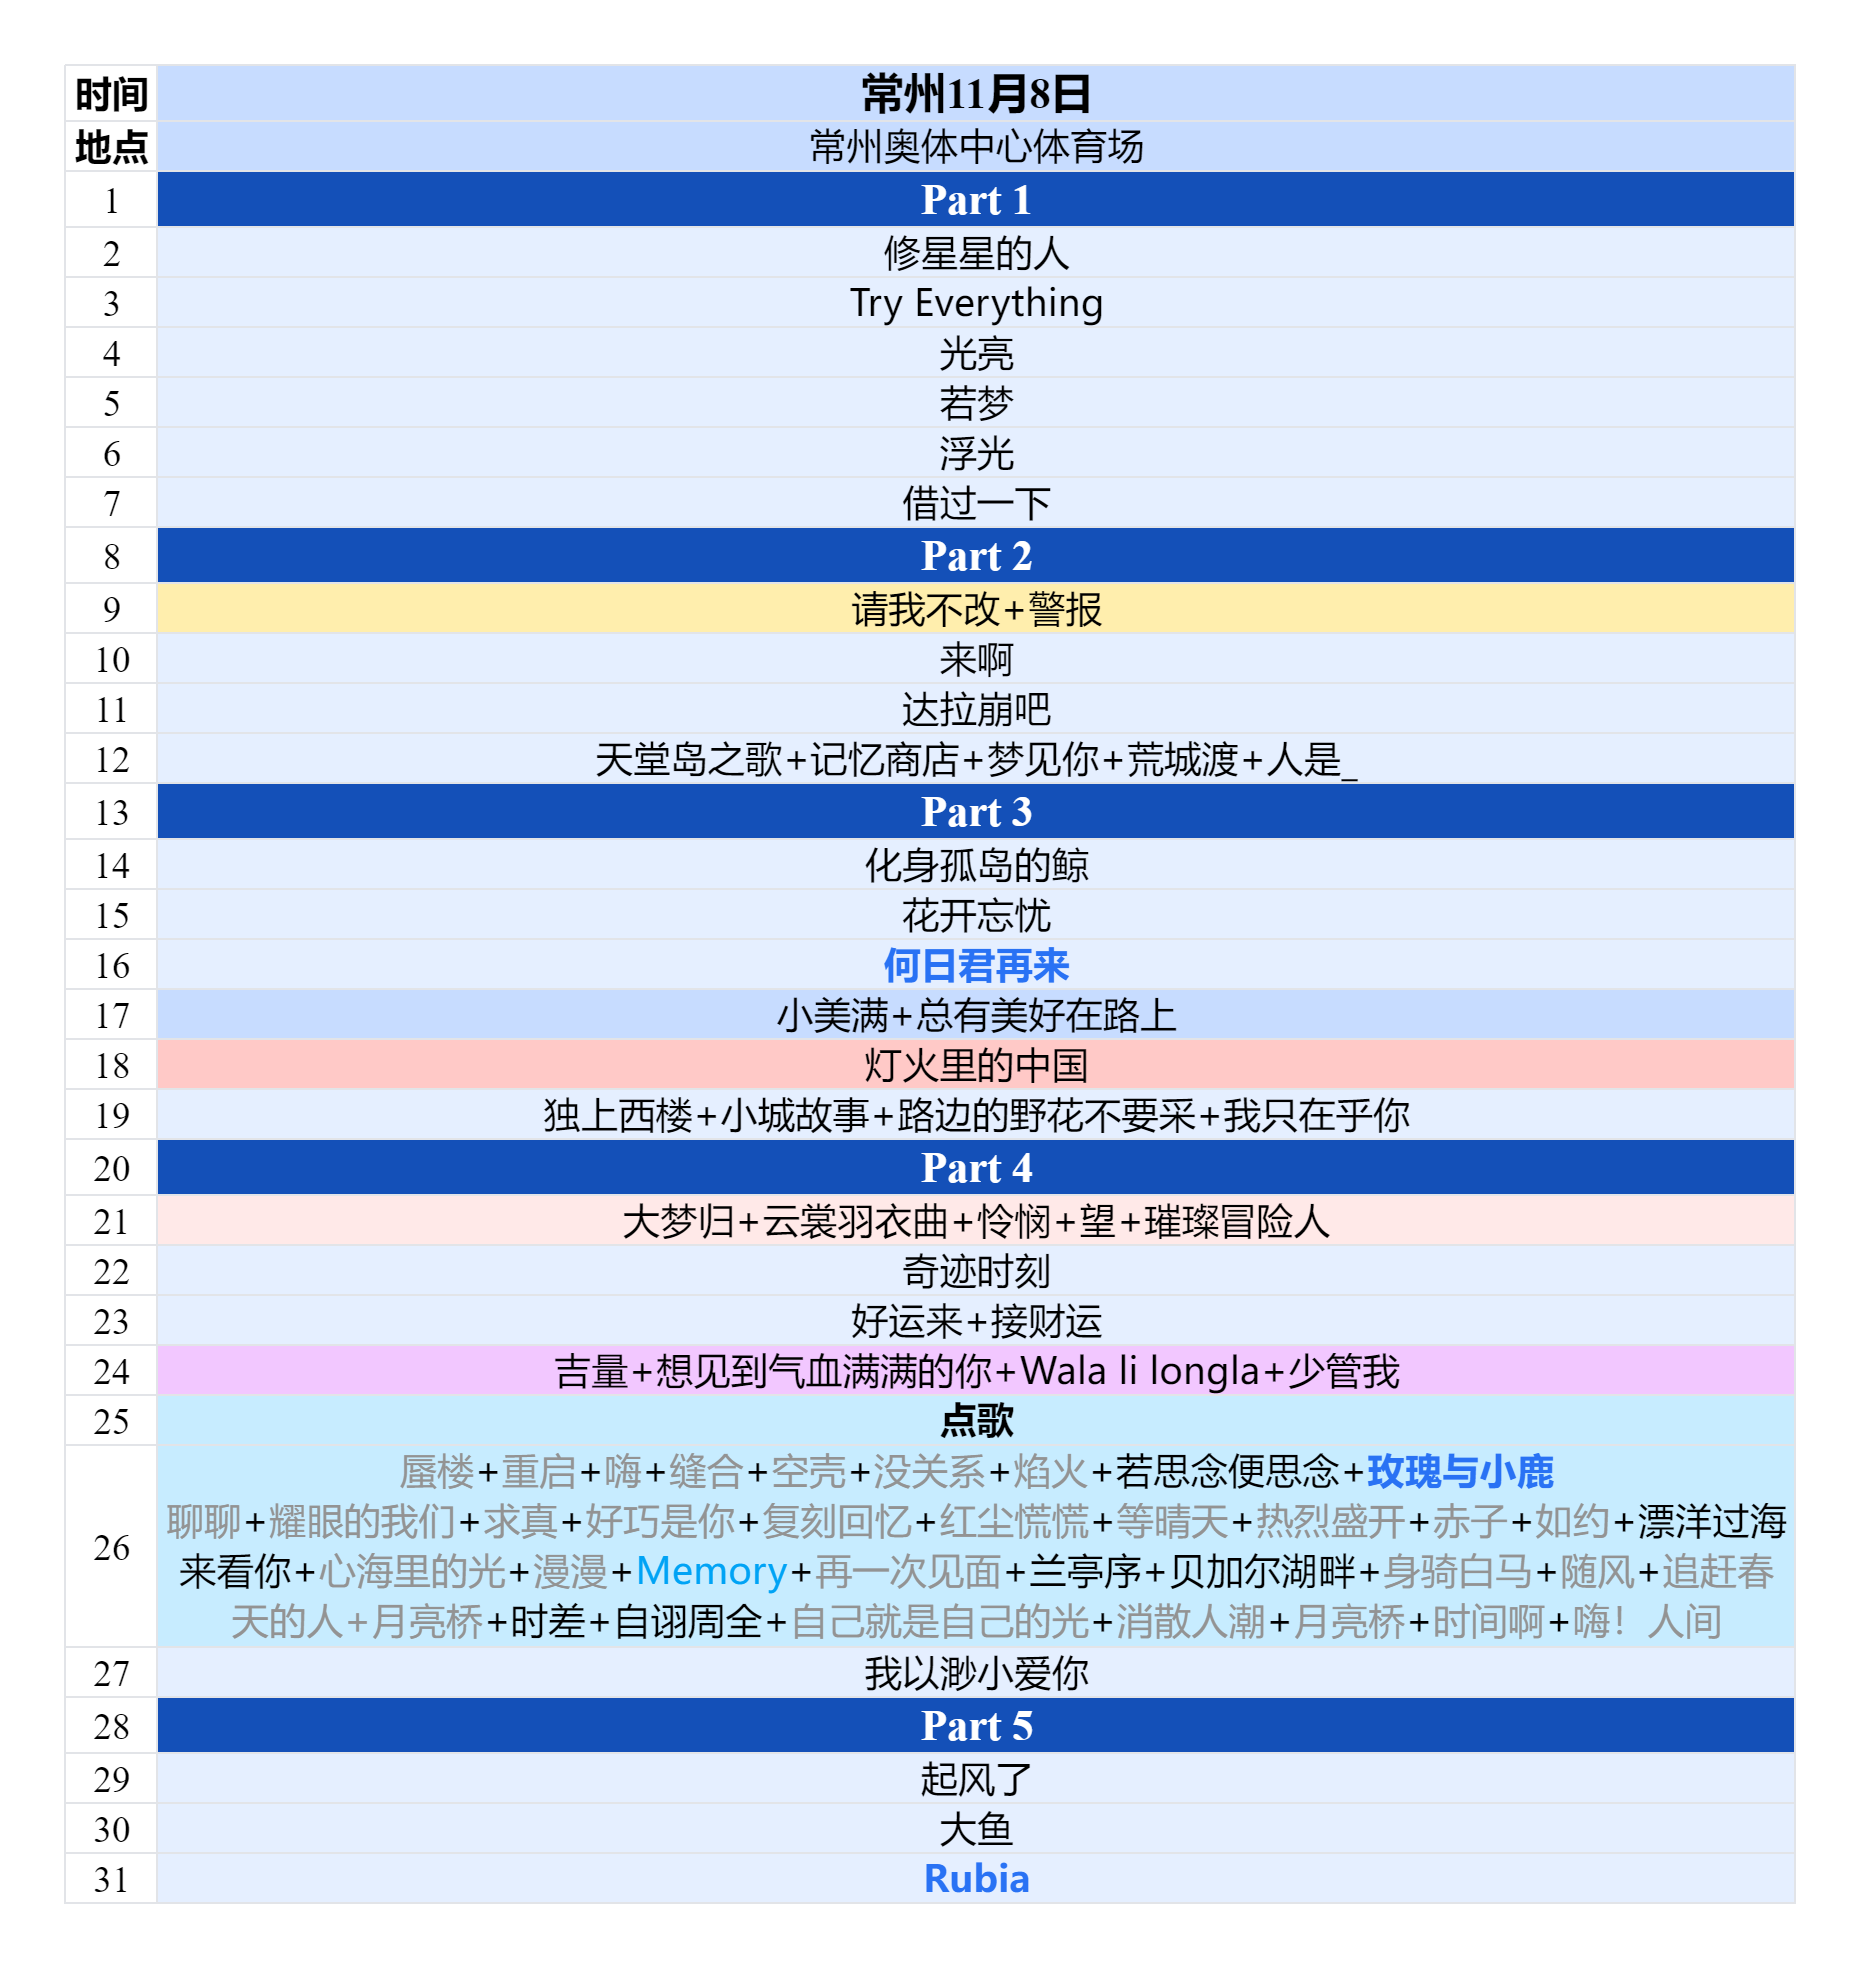
\includegraphics[width=280pt]{img/playlists/ChangZhou-20261108} 

}

\caption{2026周深“深深的”巡回演唱会2026.11.08常州场歌单}\label{fig:unnamed-chunk-60}
\end{figure}

\newpage

\section{Part1}\label{ChangZhou-20261108-part1}

\hyperref[opening-vcr]{🎥【\textbf{开场VCR}】}

\hyperref[xiu-xing-xing-de-ren]{🎵【\textbf{修星星的人}】}(深：我的情感和三十六度的体温，足以暖热即将熄灭的恒星)常州的朋友们，你们好吗？(米：啊啊啊)(深：给生命升一簇篝火)尖叫声(深：既然这宇宙让我诞生)。

\hyperref[try-everything]{🎵【\textbf{Try Everything}】}常州的朋友们你们好吗？(米：好)既然这个宇宙让我们诞生〕，我们就勇敢的try everything好不好？(米：好)让我听到你们最大的声音！后面的朋友，你们好吗？Oh oh oh oh oh，到你们(米：try everything)Oh oh oh oh oh，再大声(米：try everything)后面的朋友，(米：try everything)。

  芜湖\textasciitilde 哇\textasciitilde 太开心了，我们又见面了。常州的朋友们，你们好吗？(米：好！)谢谢你们来跟我们见面，也一定要好好照顾好自己，多穿一件衣服好不好？(米：好！)欢迎大家来到深深的巡回演唱会，这是我的一本人生日记，你会发现哇它好精彩，那为什么它那么精彩呢？就是由每一个最美好的你们帮我组成的，所以再一次非常感谢你们让我的人生变得这么的精彩，谢谢你们！(米：谢谢深深！)不对，是谢谢你们，没有你们的话我们真的做不到，再次感谢大家。

  来到常州，又要说几句常州话，如果我说的像常州话的话，给我一点点鼓励吧。(米：好！)【常州话环节】常州个朋友们，大家好，我是周深，阿拉又见面了。昨天来过个人举举手我看看呐，差点汗流啊。各位都嗨起来哦。有这么不标准吗？欢迎大家来到深深的巡回演唱会！

  哇，真的很难学，而且我们这一片的语言，它有很多地方方言它很很像，但是它又很不一样，外地人真的是被难到了。但是呢，哪怕天色有点暗，我发现我的眼前都是非常非常的刺眼的，因为你们身上的光亮实在是太耀眼了。一定要记住，在照亮我的孤单的同时，也要照亮好你们的每一个角落，好吗？(米：好！)谢谢你们愿意成为我的光亮，谢谢你们的出现。(米：谢谢周深)

\hyperref[silver-linings]{🎵【\textbf{光亮}】}到你们(深：用尽了，米：全力，努力地回应，再无边再无尽再无解总有一线生机。深：光亮你自己，\textbf{\textcolor{red}{我爱你~}})谢谢你们。(深：无论目的，最无畏的你)谢谢你们，后面的朋友，谢谢你。

\hyperref[like-a-dream]{🎵【\textbf{若梦}】}跟你们相遇这件事情美好的就像做梦一样，等一下大声的跟我一起唱若梦好不好？(米：好！)\ldots\ldots 到你们！(米：往事流转在你眼眸)再大声！(米：一边遗忘一边拼凑，如我虔诚合十双手，唯愿你能得到拯救)你们唱的太好听了！\ldots\ldots 最大声！(米：往事流转在你眼眸，一边遗忘一边拼凑，如我虔诚合十双手，唯愿你能得到拯救)全场最大声！，(米：往事流转在你眼眸)(深【和声】：在你眼眸\textasciitilde\textasciitilde\textasciitilde)(米：一边遗忘，一边拼凑)(深【和声】：一边拼凑\textasciitilde\textasciitilde\textasciitilde)(米：如我虔诚合十双手)(深【和声】：合十双手\textasciitilde)(深、米：唯愿你能得到拯救)(深：唯愿你能，得到拯救)(深：因为常州的你，你你你你你\ldots，你们，周深才得到拯救------)

\hyperref[floating-light]{🎵【\textbf{浮光}】}人生恍惚三万天！当我听到你们大合唱的时候，我脑海当中出现了个表情包：This is music！谢谢你出现在了我的生命当中，谢谢你！\ldots\ldots 最大声！(米：浮光掠影重山彩云间)再大声！(米：你的伏线穿越千百年)后面的朋友！(米：人生不过恍惚三万天)

\hyperref[excuse-me]{🎵【\textbf{借过一下}】}谢谢你们给我的力量，让我能够在寻找自己的路上说一声借过一下。(深：潇洒不是不怕，是愿付出代价)你们愿意吗？(米：愿意！)\textbf{\textcolor{red}{我爱你们}}！让我听到你们最大的合唱声(深：让我大醉一场，米：殿堂之上，背闲诗两三章)，再大声！(深、米：让我穿白衣裳，米：过疯人巷，去泥潭捞月光，深、米：望大人们见谅，)怎么了？(米：提点的话，我懂也不想装)(深米：世人寻黄金乡，米：我找月亮，何必同往。)最大声(米：话谢过，路借过，你是你，我是我)最大声(米：话谢过，路借过，你是你，我是我)。太棒了！(深：当披上月光，走夜晚)你们就是我要找的月光，我找到你了！

\section{Part2}\label{ChangZhou-20261108-part2}

\hyperref[robot-vcr]{🎥【\textbf{机器人VCR}】}

\hyperref[brave-heart]{🎵【\textbf{请我不改}】}常州的朋友们，你们好吗！(米：好！宝贝)宝你们个头啊！(米：哈哈哈)。尖叫声(深：请我不改，米：嘿！)(深：Brave heart)到你们。
\hyperref[jing-bao]{🎵【\textbf{警报}】}(深：我发送警报声，血红色惊叹号\ldots\ldots 从借用到利用到滥用\ldots\ldots)。尖叫声(深：请我不改，米：嘿！)。

  喔噢\textasciitilde 接下来这首歌是想要你们帮我一起唱，叫《来啊》，是不是有很多的朋友没有听过？(米：听过！)听过的声音很小声，那让我们来学一下，假装听过的声音很大声，哈哈哈。这首歌很很很很简单学啊，就是我唱''Don't tell me''，你们就要帮我唱``来啊啊啊啊啊，来啊啊啊啊啊''，好不好？(米：好！)后面的朋友好不好？(米：好！)试一下喽。(深：Don't tell me)(米：来啊啊啊啊啊，来啊啊啊啊爱)哎呦，有的朋友已经学会喽，我们再来一遍啊。(深：Don't tell me)(米：来啊啊啊啊啊，来啊啊啊啊啊) 哇，太棒了！那这首歌可就靠你们了哟。大家喜不喜欢来深深的巡回演唱会呀？(米：喜欢！)要不要再来常州玩呀？(米：要！)那就来啊！

\hyperref[lai-a]{🎵【\textbf{来啊}】}一起来(深：Don't tell me，米：lie eeeeeeee)，再来(深：Don't tell me，米：lie eeeeeeee)。(深：随你，操控)\textbf{\textcolor{red}{我爱你们}}。(深：我望眼欲穿你别闪躲)再来。

  接下来到了我们深深的巡回演唱会的小游戏环节。大家可以通过你们喜欢的颜色去变换我们的荧光棒，分别是粉色、黄色、蓝色和绿色，给大家五秒钟选择的时间。没有红色。(米：有！)粉红色，哈哈哈。所以有红色吗？(米：有！)行行行，你们是这里的主人，你们说了算，那我们就把红色按照粉红色来计算。不同的颜色代表着不同的角色，蓝色代表的是达拉崩巴。(米：哦！)红色代表的是国王陛下以。粉色代表的是公主米娅，那绿色代表的就是恶龙，他终于来到了我们的龙城常州。让我们一起欢迎恶龙，嗷呜嗷呜，三二一。(米：嗷呜！嗷呜！)很棒。没错，所有的角色都跟刚才恶龙一样有它相对应的台词。所以，没事不用藏我的秋衣。哈哈哈，你们有穿秋衣吗？(米：没有！)还有人摇头。大家要记得穿秋衣和\ldots\ldots(米：秋裤！)好不好？(米：好！)

  好的哟。相对应的角色有相对的台词，所以当我喊到你的角色，你就要喊出他的台词哟。达拉崩巴！(米：我最棒！)国王陛下！(米：再说一次！)公主米娅！(米：救我啊！)恶龙！(米：啊呜啊呜！)哦，我知道红色代表什么意思了。(米：宝贝！)你们知道我们工作室的名字叫什么吗？叫劲焱(``禁言'')。红色的朋友是不想浪费自己的嗓子跟我们互动是不是？你们什么意思？所以当我喊红色，我喊常州！(米：宝贝！)，我没有让你们喊宝贝这两个字，累了。常州！(米：宝贝！)人生啊，起起落落。达拉崩巴！(米：我最棒！)国王陛下！(米：再说一次！)公主米娅！(米：救我啊！)达拉崩巴！(米：我最棒！)国王陛下！(米：再说一次！)公主米娅！(米：救我啊！)公主米娅！(米：救我啊！)公主米娅！(米：救我啊！)恶龙！(米：啊呜！)恶龙！(米：啊呜！)恶龙乘以十，走！(米：啊呜！啊呜！啊呜！啊呜！啊呜！啊呜！啊呜！啊呜！啊呜！啊呜！)常州！(米：宝贝！)后面的朋友们，常州！(米：宝贝！)不知道发生什么事情了，后面莫名其妙跟着一起喊宝贝，你们不觉得奇怪吗？哈哈哈。那就跟我一起来复述一下达拉崩巴这个童话故事吧。

\hyperref[dalabengba]{🎵【\textbf{达拉崩吧}】}荧光棒！全场，达拉崩巴！(米：我最棒！)国王陛下！(米：再说一次！)公主米娅！(米：救我啊！)恶龙！(米：啊呜啊呜！)达拉崩巴！(米：我最棒！)国王陛下！(米：再说一次！)公主米娅！(米：救我啊！)常州！(米：宝贝！) 达拉崩巴！(米：我最棒！)国王陛下！(米：再说一次！)公主米娅！(米：救我啊！)恶龙！(米：啊呜啊呜！) 恶龙！(米：啊呜啊呜！) 常州！(米：宝贝！)后面的朋友。他的全名是，达拉(米：崩吧斑得贝迪卜多比鲁翁)救出了(米：公主米娅莫拉苏娜丹妮谢莉红)常州！(米：宝贝！)这么爱念，(深：要念你来念吧)尖叫声。

  哇！你们太厉害了。大家有吃萝卜干炒饭吗？(米：有！)真的很好吃，好吃到什么地步？我这几天每一顿吃的饭都是萝卜干炒饭。哈哈哈，当然会有一点其他的菜啊，但那个萝卜干炒饭真的太太好吃了，大家不要错过好不好？(米：好！)哎呦。那在前年我发了一张专辑，它叫做------(米：反深代词！)《反深代词》那个世界不经常下雨。哈哈哈，现在有点毛毛雨了，大家可以把雨衣穿一下，不要生病了，好不好？(米：好！)怎么还有不好的？哈哈哈。好，《反深代词》这张专辑说的是两百年后的世界，那个世界叫做反深代词，周深一共有十二个不同的情绪碎片，也就是说这张专辑当中有十二首不同的歌，代表着周深不同的情绪碎片。如果你在听这张专辑的时候，你发现，诶，某首歌的经历跟你的感受，跟你的情感简直一模一样的话，那证明我们在两百年后的这个反深代词世界里面彼此相互拥抱，认出彼此了，好不好？(米：好！)我喘一口气，在今年它的实体专辑也发行喽，谢谢大家的支持，也谢谢大家能够给我足够的勇气去做这样一张专辑。因为这张专辑它是非常全面的去剖析自我的一张专辑，大家也都知道，看见自我和愿意去剖析自我是需要勇气的事情，所以谢谢你们给了我这样的勇气。然后也希望没有听过的朋友可以在线上去听一下，好不好？(米：好！)那在反深代词这个世界有一栋楼，它叫做蜃楼，它是有很多执念组成的这样一栋楼。哦，那后面还发生了些什么事情呢？我们一起来看一下吧。

\hyperref[haven-song]{🎵【\textbf{天堂岛之歌}】}生米们，你们在吗？(米：在)听过周深唱歌的朋友们你们在吗？
\hyperref[the-memory-store]{🎵【\textbf{记忆商店}】}哎，这是深深的巡回演唱会吗？(米：对！)哦，这是《反深代词》当中的记忆商店。哎，我梦里梦到过这样的场面，但是记忆商店里面的人，他没有做这个颜色的美甲呀。你看大拇指露出来了。哦，做美甲为什么只做一只啊？记忆商店的人好奇怪呀。哦，我知道了，只要拥有这一颗米子心，就可以唤醒我们最喜欢的那段回忆。啊，但是记忆商店里有太多我们美好的回忆了，因为跟你们相遇的每一分每一秒都值得被收藏，那我们一起来看一下好不好？(米：好！)你们想看这个\ldots\ldots 你藏的那么深我也看见你做了美甲了，哈哈哈。你们想看只做一只美甲的那个记忆，还是全套美甲的这个记忆呢？(米：一只！)一个的是吗？(米：对！)为什么做的是绿色不是蓝色？
\hyperref[meng-jian-ni]{🎵【\textbf{梦见你}】}又是你们这群黑竹荪。(深：看着眼前，还年少的你)。居然用这么肮脏的手段，你们都是我的宝贝。谁不会啊？哦，哦，这么大！这是个真的常州恐龙蛋，我隐约看见里面有一只小恐龙？大家想不想看一下我们的黑竹荪。下面的朋友？(米：想！)准备好了吗？(米：准备好了！)你准备好，你好敬业呀。我们一起来看一下好不好？这怎么\ldots\ldots 哎呦。等等，你们是看\ldots\ldots{}
\hyperref[huang-cheng-du]{🎵【\textbf{荒城渡}】}(米：会！)嗷呜嗷呜。
\hyperref[Humans_are_]{🎵【\textbf{人是\_}】}和我一起唱，(深：让时空消亡我)唱(米：你无需记得我)(深：来摧毁我深爱的一切，可仍夺不走我的选择)再来(深、米：弹指间湮灭我，但命运打不败活着)。在遇到你们之前，我也被困在记忆商店，我认为那些失去的、过去的才是最美好的。但是因为听到了你的歌唱，``This is music''，(米：哈哈哈)我才明白，哎我这段很认真耶，我才明白我们现在拥有的每一分每一秒才是最宝贵的，你们说对吗？(米：对！)谢谢你们创造了不朽的、永恒的爱。【不朽的，永恒的，我们记得，不朽的，永恒的，我们记得。】

\section{Part3}\label{ChangZhou-20261108-part3}

\hyperref[music-animations-vcr]{🎥【\textbf{音乐动画VCR}】}

\hyperref[The-whale-who-became-an-island]{🎵【\textbf{化身孤岛的鲸}】}。(米：周深我爱你。米：哇哦)你们好啊！(米：好！)为什么会突然``哇哦''？到你们(米：你的衣衫破旧，而歌声却温柔，陪我漫无目的的四处漂流)后面的朋友。你们，(米：你与太阳挥手，也同海鸥问候)。(深：我想给你能奔跑的岸头)(米：没有墙头)。(深：欢迎大家来到了常州。你的心里却装着些你的墙头。)(米：没有)很多朋友应该很疑惑，啊？他们在说什么？我说你们心里装着你们的墙头。我解释一下什么是墙头啊，就是当我问生米们，你们喜欢哪个歌手啊？(米：周深)他们会说，周深，或者是宝你的头，啊。然后呢，我就会说，哎，我真的很讨人厌，就非要问人家，那你们还喜欢其他歌手吗？(米：没有！)你看，他们就会像现在这样骗我，说没有。其实他们，嗯\ldots\ldots 哎呦，我都不说，不好意思说。所以我就非常不礼貌地把他们喜欢的歌手称为墙头，的确非常没有礼貌，大家不要学我。但是(深：无论你们有多少个墙头)，你们都是(深：我的国王和王后)。谢谢你们看到了我。(米：谢谢周深)

\hyperref[Blossoms-that-forget-sorrow]{🎵【\textbf{花开忘忧}】}常州的朋友们，我们来常州看你咯！(米：哇！)(深：巷子口买了花，穿过沿街红墙青瓦)。(深：若记忆被偷走了，忘了我的爱，我会说)说什么？(米：你好啊)你们好吗？(米：好)(深：这是给你的花，花的名字叫忘忧草，它说时光汹涌如水上烟波，别走远了一起回家)我们一起回家好不好？(米：好)一定要好好照顾好自己，好不好？(米：好！)来，让我们一起。(深：我们苍老的时候，米：就回到小时候，采青梅用来酿酒你不许偷着喝，穿朴素的衣裳牵着那衣袖，捡了小猫名为苍狗)再大声。

  在我们的人生当中，一定有那么一个非常非常重要的人，也住着一份遗憾，我们可能再也没有机会见到他。但是我相信，只要我们的思念够大声，他一定听得到，你们说对吗？(米：对！)所以我们一定要好好的照顾好自己，因为他也一定感受得到，你们说对吗？(米：对！)花开忘忧，愿你无忧。花开忘忧！(米：愿你无忧！)谢谢你们。(米：谢谢周深)哇，太幸福了，我好开心啊！后面的朋友们，你们好吗？(米：好！)

  这是我第一次来到常州开演唱会，就是连续开两天体育场，就真的不真实的跟一场梦一样。然后关于常州的歌，我自己昨天有一首自己的歌，你们会唱吗？(米：会！)(深：我会热烈的，米：热切地盛开，开在荒野开在小小角落与人海，山有其巍峨，我有我姿态，向阳而生会有光为我而来。我用绚烂骄傲的盛开)再大声，(米：开在山巅开在山花烂漫的花海，我要奔赴我的热爱，要万里长风为我喝彩。)

  那今天要唱的这首歌呢，跟我也非常非常的有缘分，因为这首歌的原唱也姓周。这首歌很多人听过，但是听的可能会是我自己的偶像邓丽君女士的版本，这首歌叫《何日君再来》，有人听过吗？(米：听过！)那这首歌的原唱周璇是我们常州的朋友哦，所以等一下跟我一起大声的唱好不好？(米：好！)

\hyperref[he-ri-jun-zai-lai]{🎵【\textbf{何日君再来}】}这一次见面之后，你们会忘了我吗？(米：不会！)那我们还要相聚在深深的好不好？(米：好！)我们还要再相聚在常州好不好？(米：好！)后面的朋友。(深：好花不常开，好景不常在)到你们。(深：来来来，喝完这杯姜汤再说吧。〔现场把``喝完这杯再说吧''即兴改成了姜汤版〕)亲爱的朋友们，天气有点冷，希望大家就是需要的话，喝一下我们现煮的姜汤好不好？(米：好！)(深：停唱阳关叠，)到你们(米：重擎白玉杯，殷勤频致语，)照顾好自己(米：牢牢抚君怀。)再大声。哎，姜汤虽好，也不要贪杯哟。我们一定会珍藏我们创造的这一份美好的回忆对不对？(米：对！)我们一定还会再见面的对不对？(米：对！)那这一首歌你会唱吗？(米：会！)

\hyperref[simple-bliss]{🎵【\textbf{小美满}】}来来来，唱完这首小美满吧。(深：没什么大愿望)唱！(米：没有什么事要赶)后面的朋友，(米：乌云还挺大胆)怎么了？再来。全场跟我一起唱哦。大声唱。谢谢你们(米：谢谢周深)。(深：笑一笑就灿烂)唱。(米：没道理的开朗)怎么了。最大声！因为跟你们相遇，我真的真的好幸福啊！

  让我们一起在小美满这一首歌当中一起许愿吧。我给大家举个例子，像我这样闭上眼睛，然后想好你心中的愿望，我会倒数三二一，当你睁开眼睛，我们的愿望就会出现在这棵许愿树上。现场无论什么年龄段，无论什么职业的朋友，所有人闭上眼睛许愿咯。想一想生日的时候第一个蹦出来的愿望是什么呢？想一想一直想要实现的愿望是什么呢？哦对了，小美满这首歌当中的愿望只能够许关于自己的愿望。想一想是不是很久没有转身看一看一直在努力的自己了？想一想是不是从来没有跟自己说一声你真的真的很棒，你真的真的已经尽力做到非常非常好了？想一想是不是从来没有跟自己说一声我真的好爱你啊，我要好好照顾好你？三二一，睁开眼睛，我们的愿望一定会实现的对不对？(米：对！)(深：笑就好，哭也好)到你们(米：自己就是自己最好的陪伴)，(深：你们都是周深最好的陪伴)，因为你的出现，每一天都非常非常特别，我也感受到了你的善意。

  让我们一起祝今天生日的朋友！(米：生日快乐！)你们太美好了。让我们祝昨天或者是前一段时间过生日的朋友！(米：生日快乐！)让我们一起祝明天或者过一段时间生日的朋友！(米：生日快乐！)

\hyperref[zong-you-mei-hao-zai-lu-shang]{🎵【\textbf{总有美好在路上}】}。因为你的出现，我才感受到了(深：花在开，云在飘，笑容在脸上，我们向前方一路向阳)到你们，(米：亲爱的你，在路上慢慢逛)。(深：抬头发现，你们都是光芒)。

\hyperref[deng-huo-li-de-zhong-guo]{🎵【\textbf{灯火里的中国}】}灯火里的中国，美不美丽？(米：美！)那也是由最美好的你组成的，你非常重要，你要记得，好不好？(米：好！)跟我一起唱好不好？(米：好)大声唱。再大声。大声唱。

  你们唱歌太好听了。哇，你昨天高音练得怎么样？他说他，他说他有练。您作为一个很厉害的摄像老师回去练高音干嘛？想要唱给大家听。哦，我感受到了，大家想听吗？(米：想！)今天要比昨天更进步一点好不好？今天比昨天进步一点好不好？来，我来拍你啊，你看你身后空无一人，不要再找他们了，你的伙伴们已经抛弃了你。来喽。还是一样的，前面那部分还可以，你前面完成得很好。(深：啊\textasciitilde)(摄像老师：啊)，鼓励！(深：啊)加油，你肌肉练得那么大块。那他比昨天好有没有，对不对？掌声鼓励他，我的生米们很厉害的。(深：啊啊，米：啊啊啊)是不是很厉害？那就再听一遍好不好？(深：灯火里的中国，米：青春婀娜，深：灯火里的中国，米：胸怀辽阔)大声唱！(米：灯火里的中国，青春婀娜\ldots)(深：灯火荡漾着心中)唱(米：的歌)(深：This is music)给自己鼓励！(米：喔！)

🎵【\textbf{邓丽君组曲}】\\
  我会继续好好唱歌，希望可以成为像邓丽君女士这样的歌手，有好多歌去陪伴你们。很开心自己有这样一个目标，但我更幸运的是能够被你们听见和看见，陪我去寻找那个自己。谢谢你们的出现！(深：谢谢周深)。如果会唱的话，等下跟我一起大声唱好不好？(米：好！)

\hyperref[du-shang-xi-lou]{🎵【\textbf{独上西楼}】}(深：无言独上西楼，月如钩\ldots\ldots 是你们的墙头)(米：没有！)(深：还在骗我说没有，你们到底有多少个墙头？)(米：没有！)
\hyperref[xiao-cheng-gu-shi]{🎵【\textbf{小城故事}】}我们现在在的城市是------(米：常州！)一起唱！(深：常州故事多)怎么了？(米：充满喜和乐，若是你到常州来，收获特别多)大声唱！(米：看似一幅画，听像一首歌，人生境界真善美，这里已包括)。怎么说啊？(米：谈的谈，说的说，常州故事真不错，请你的朋友一起来)来哪里？(米：常州来做客)你们来邀请！(米：请你的朋友一起来)来哪里？(米：常州来做客)
\hyperref[donot-pick-the-roadside-flowers]{🎵【\textbf{路边的野花不要采}】}这首歌会唱吗？(米：会！)让我听到最大的声音哦，预备起！(深：送你)(米：送到小村外，有句话儿要交待，深：虽然已经是百花开，路边的野花)，他怎么了？(米：你不要采)。你们听到了吗？唱！(深：记着我的情记着我的爱，米：记着有我天天在等待)大声唱。(深：千万不要把我来忘怀)。
\hyperref[I-only-care-about-you]{🎵【\textbf{我只在乎你}】}谢谢你们。我经常会被问到一个问题，如果你没有当歌手，你在做什么呢？我真的也没有找到任何答案。(深：如果没有遇见你)。(深：任时光)(米：匆匆流去，我只在乎你，心甘情愿感染你的气息)大声唱！(米：人生几何)怎么了？(米：能够得到知己)。全场最大声！(米：任时光匆匆流去，我只在乎你\ldots\ldots)再大声！(米：人生几何能够得到知己)。你们(米：除了你，我不能感到一丝丝情意)再来最大声！(米：除了你，我不能感到一丝丝情意)你们会忘了我吗？(米：不会！)(深：除了你，我不能感到一丝丝情意)。我只在乎你。谢谢你们。(米：谢谢周深)。

\section{Part4}\label{ChangZhou-20261108-part4}

\hyperref[mask-vcr]{🎥【\textbf{面具VCR}】}

(VCR：我相信我们一定能找到属于自己的答案的，你说，对吗？)(米：对！)〔回应VCR结尾〕没听到哦。(米：对！)你说，对吗？(米：对！)

\hyperref[da-meng-gui]{🎵【\textbf{大梦归}】}你们会跟我一起大声唱的，对吗？(米：对！)(深：春尽枝头慌，再一季)。你们会唱吗？(米：会！)让我听到。(深：就让冷风吹，米：雨纷飞，留一地伤悲)再大声(深：就让爱破碎，米：恨成灰，往事都作废，深：就让火一堆，米：酒一杯，送一袖清晖)。
\hyperref[Song-of-the-cloud-dress]{🎵【\textbf{云裳羽衣曲}】}我们的缘分一定不会太浅，因为我的名字叫？(米：周深)我们巡回演唱会的名字叫？(米：深深的！)我们要把歌唱得越来越大声，好不好？(米：好！)(深：故事鲜艳而缘分却太浅，米：我的爱恋，竟如此的明显)。再大声。谢谢你们！(米：谢谢周深)。
\hyperref[lian-min]{🎵【\textbf{怜悯}】}我们不要祈求怜悯，我们都要好好的照顾好自己，不要生病，我们都值得被好好的爱着，对不对？(米：对！)一起唱吧。
\hyperref[Expectation]{🎵【\textbf{望}】}(深：我们总会绕啊绕，绕啊绕)唱！
\hyperref[adventurers]{🎵【\textbf{璀璨冒险人}】}璀璨冒险人们，你们准备好了吗？(米：准备好了！)跟我一起向前冲吧！好不好？(米：好！)(深：如果得不到谁的认同那就不算拥有)你们(米：没人能够决定谁的一生应该怎么活)。你们都是我的英雄！谢谢你们！(深：就让一路曲折，每一道伤口洗净我的脆弱)最大声！再大声！(深：要炙热啊！要不忘啊！要勇往啊！起风了，不安了，你还在等什么？挥手了，再见了，别不舍回头啊。向心中的梦啊，去追吧。要能留下伤痕才算活过，愿你记得，愿你哭过，不惧脆弱，不惧脆弱，不惧脆弱)。希望你永远无畏，永远有勇气，也永远要用那一份最炙热的爱，拥抱那一个敢于挑战的自己。千万不要害怕看到自己脆弱的一面，因为脆弱的那一面也是组成最完美的我们的一部分，对不对？(米：对！)希望你工作顺利，生活顺利，学业顺利，也(深：不惧脆弱)。

  当我们相遇的每一分每一秒，都叫做奇迹时刻。

\hyperref[miracle-moment]{🎵【\textbf{奇迹时刻}】}荧光棒。你们好吗？
  我要准备变魔术啦！(米：好！)我的魔术现在已经越来越厉害了，特写机位上来。大家看，这是一个很普通的一个小盒子对不对？然后里面是哎呦哎呦哎呦，非常普通对不对？现在我把这三个硬币放进去，那如果我把这张纸这样拦住，把它卡住的话，是不是等一下我把这三支铅笔穿过去是不可能的事情对不对？(米：对！)倒数三秒，三、二、一，尖叫声！(米：wow！)更神奇的是，我们还能复原，三、二、一！再来看哦，这是一个球对不对？一个皮筋，还有一个非常普通的一个铁圈圈，和一个普通的丝巾。我们现在呢把这个球放在这个丝巾中间，让这个球是逃不出来的对不对？(米：对！)然后我们再把这个丝巾穿过这个铁圈圈当中，没有问题吧？(米：没有！)厉害的是什么？厉害的是我这个魔术非常浪费时间。如果我现在把这个球放到这个杯子当中，我等一下可以直接把这个铁圈圈直接就隔空把它取出来，你们相信吗？(米：相信！)相信？相信那我就不变了。相不相信？(米：不相信！)你们最好相信我一下，不相信我会搞砸的。没有问题吧？(米：没有！)倒数五个数字，大家看好检查没有任何问题对不对？没有啊，我会隔空直接把这个圈圈就变出来，大家看好，没问题啊，来，五、(米：四、三、二、一！)(话筒)为什么卡住了？想来看周深变魔术笑话的人，让你们失望了，技术已经不允许我失误了。那好运来了你们接不接？(米：接！)我厉不厉害？(米：厉害)

\hyperref[good-fortune-comes]{🎵【\textbf{好运来}】}大声唱！唱！再大声！常州的朋友们，身体健康接不接？(米：接！)恭喜发财接不接？(米：接！)大声唱！唱！再来一次！唱！常州的朋友们，好运来了接不接？(米：接！)等一下用最大的声音跟我接所有的美好祝福好不好？(米：好！)
\hyperref[jie-cai-yun]{🎵【\textbf{接财运}】}我们一起接平安，唱！(米：接平安！)我们一起接幸福！(米：接幸福！)接健康！(米：接健康！)接财运！(米：接财运！)接不接？(米：接！)常州的朋友，祝你们恭喜发财，接不接？(米：接！)

  哦？二位是\ldots\ldots 我们帮我们常州恐龙园辟谣一下，里面不是这个样子的，大家有机会去玩一下好不好？(米：好！)那我就要坐着我们的小车车来看一下，有谁没有好好的接好运哦，好不好？(米：好！)祝大家依然在马年拥有无量的吉祥，希望你们身体健康，生活顺利，工作顺利，学业顺利，最重要的是好好照顾好自己好不好？(米：好！)

\hyperref[ji-liang]{🎵【\textbf{吉量}】}吉量你们会唱吗？(米：会！)让我听到你们的声音哟。欢迎大家来到常州！一起，(深：望舒驾后银尾巴)你们。你们好。hello。生米朋友你们好。全场！你们好吗？

\hyperref[xiang-jian-dao-qi-xue-man-man-de-ni]{🎵【\textbf{想见到气血满满的你}】}哈喽！提问(深：你是谁？你是自己的)(米：宝贝！)宝贝(深：要时刻感觉自己多珍贵)你是最珍贵的！(深：还会有更好的等着你，还有好多梦在飞，还要给自己一个新的机会)你们好！(深：要早起早睡，别那么累，做好气血满满的准备。想见到你，灿烂的你，无惧也无畏。别害怕疼痛，别怕眼泪，就让我来陪着你找回，手里有暖，心里有暖，阳光的明媚。有再疼再冷再怕的时候，请你一定记得，我永远会是你永远的选择。为有梦可贵，勇气可贵，举起热情满满的奖杯，那时的你，灿烂的你，无惧也无畏。)提问，(深：你是谁？你是自己的？)(米：宝贝！)你是自己的？(米：宝贝！)常州的宝贝们你们好吗？(米：好！)糟糕了，我居然已经开始心平气和的说出``宝贝''这两个字。宝你们个头！

\hyperref[wala-li-longla]{🎵【\textbf{Wala li longla}】}在我的专辑《反深代词》当中有一个快乐密码，喊得越大声，快乐来得越快，我们等下一起喊好不好？(米：好！)我们学一下哟，谢谢您。Wala li longla！(米：Wala li longla！)这边的朋友，Wala li longla！(米：Wala li longla！)全场，Wala li longla！(米：Wala li longla！)(深：把蜗牛都放大，把汽泡堆成塔)你们好！你们好！常州的朋友们，让我们一起喊出这个快乐密码，帮我一起喊出来好不好？(米：好！)来喽！Wala！(米：Wala！)Wala li！(米：Wala li！)这边咯，Wala li long！(米：Wala li long！)Wala li longla！(米：Wala li longla！)Wala！(米：Wala！)Wala li！(米：Wala li！)Wala li long！(米：Wala li llong！)Wala li longla！(米：Wala li longla！)Wala！(米：Wala！)Wala li！(米：Wala li！)Wala li long！(米：Wala li llong！)Wala li longla！(米：Wala li longla！)Wala！(米：Wala！)Wala li！(米：Wala li！)这边的，Wala li long！(米：Wala li llong！)Wala li longla！(米：Wala li longla！)你们好！Hello，你们好，全场最大声！(深：Wala li longla！)你们(米：Wala li longla！)

\hyperref[watch-ur-manners]{🎵【\textbf{少管我}】}我们还有一个暗号，三二一，嘿，少管我。三二一，嘿！(米：少管我！)全场最大声，三二一，嘿！(米：少管我！)你们好吗？上面的朋友！你们好！谢谢你们来看我们！谢谢你们！谢谢你！你们好！尖叫声！三二一，嘿！(米：少管我！)你们好吗？三二一，嘿！(米：少管我！)这边的朋友，三二一，嘿！(米：少管我！)你们好！三二一，嘿！(米：少管我！)三二一，嘿！(米：少管我！)五四三二一，嘿！(米：少管我！)谢谢你们！

  哇哦！谢谢你们！哇，龙爪原来长这个样子啊。《少管我》是一首非常轻松活泼的歌曲，是想要告诉你，遇到一些烦心的事情的时候，只要你想得够清楚，在不打扰别人的前提下，就轻轻松松跟他说一句，嘿！(米：少管我！)要记住哦，成为自己这件事情没有任何人做得比你更好，所以好好的去寻找自己好不好？(米：好！)这个重要的任务可是不分任何年龄段和任何职业都要去好好做好的任务哟。

【\textbf{点歌环节}】\\
  那接下来帮我们一起点歌吧！芜湖，来，全场帮我倒数五个数字，五、四、三、二、一，停！哦哦，hello！(巧克力：宝贝你好！)宝您个头\ldots\ldots 哇，眼罩是戴在帽子上的。你好，怎么称呼您？(巧克力：我叫巧克力。)巧克力？你不会是可可烘焙坊出来的巧克力吧？(巧克力：对呀对呀。)所以你是一不小心就跑出去的巧克力大门那一扇的巧克力？(巧克力：啊，是的。)好勉强的回应，是来自哪里的朋友？(巧克力：我来自有生米的南昌。)哦，你的意思是常州没有生米吗？(巧克力：有生米大桥，在南昌。)对，我知道，开玩笑，因为我有去开过演唱会哦，你有去吗？(巧克力：那个我是听你的那个第一场演唱会。)今天这一场吗？(巧克力：啊不是，南昌。)哦，南昌的是你听的第一场，谢谢您，谢谢巧克力。那你听的第一首歌是哪首歌？(巧克力：那就《花开》吧。你可以唱两句吗？)你可以点啊，我可是开了很多场演唱会的人呢，这种套路我是不会轻易地，主要是没词儿。《花开》，哎，你帮我起个头好不好？春？今？春？副歌第一个字是哪个字？今天？现在？春暖？眼前？(巧克力：春暖花开)。刚才是一副好精彩的你画我说，下面在跟你``眼前\ldots\ldots''(深：眼前春暖花开\ldots\ldots)(巧克力：唱不上去)唱不上去你也要给我唱。(深：美在不能永恒的忐忑)(巧克力：爱你)。你怎么学会这种招数？(巧克力：跟你学的啦)我没有这样教你。是自己一个人来的吗？还是跟朋友一起来的？(巧克力：哦，姐姐在那边。)哦，跟姐姐一块儿。(巧克力：她的小恐龙。)哦，这是姐姐的小恐龙可可啊。(巧克力：对。)他叫可恐可怖的。好，给姐姐打个招呼吧，(巧克力：姐姐打个招呼)我叫你跟姐姐打个招呼，(巧克力：哦，我太紧张了)不会，好，那帮我们点出今天第一首歌喽。(巧克力：我就点《玫瑰与小鹿》吧。)把《花开》给我唱完。(巧克力：啊我\ldots\ldots 爱你)(深：眼前春暖)。(巧克力：爱你。)不要用这种手段，那在我们深深地留下你灿烂的笑脸好不好？(巧克力：我还想说几句话可以吗？)歌都不唱，话倒是要说的，你说你说你说。(巧克力：就是呃我我从来没有追过星，然后你是第一个。嗯，然后我希望你可以陪我们唱到八十岁。等你可能\ldots\ldots 呃我还想拄着拐杖去看你，然后你一定要来见我们。)

  哇，谢谢，其实真的很感动，因为就是你知道，就她在说话的时候其实声音都是抖的。还有就是昨天我们不是唱着唱着就下雨了吗？啊，我不是那个意思。这其实有很多这种就心里忐忑的瞬间，包括今天，我一个人在想哎呀，感觉好像今天天气很冷，会不会有人来跟我们见面。结果发现有很多无数个这种我没有安全感很忐忑的时刻，在我非常非常不确定的时候，我一转身发现，哇，你们还在等我，你们还在等我见面。所以衷心地感谢每一位听见我和看见我的你。谢谢每一个像巧克力这样就是一直在好好地过好自己的生活，然后还要就是一直去疯狂就是让我们彼此都成为更好的自己，我觉得这个是最最最最最重要的事情。所以一定要好好照顾好你自己好不好？我们一起成为(巧克力：深深跟生米长长久久)。谢谢，所以我们都要好好地照顾好自己好不好？(米：好！)声音不够大，好不好？(米：好！)巧克力，那在深深的留下你灿烂的笑脸吧。谢谢你们给我这么多安全感。看前面，你口罩要拿下来吗？这样拍稍微不是很好看，嗯，没有多大区别。好了，看前面喽，三二一，耶！哇，你怎么都这么好看。哦这张可以吗？不可以我们可以再重来的，你不用担心。可以是吧？谢谢巧克力，谢谢你！我们也期待你给我们写的祝福语哦，大家有看到，每一个跟我们留下灿烂笑脸的都有写祝福语，祝大家平平安安，幸福平安，快快乐乐，一定要照顾好自己好不好？(米：好！)

\hyperref[the-rose-and-the-deer]{🎵【\textbf{玫瑰与小鹿}】}玫瑰与小鹿，你们会唱吗？(米：会！)我不信，真的假的？(米：真的！)到你们。谢谢你们！

  谢谢你们在我无数个非常没有安全感的时刻，一转身都让我看见了你最温柔的光亮，谢谢你们！帮我再一次倒数五个数字吧，五、(米：四、三、二、一！)用手跟我一起倒数的人越来越多了。您好！(一苇：宝贝你好。)宝你个头，怎么称呼您？(一苇：呃我叫一苇，一苇以航的一苇。)是一苇，一苇以航的一苇。哦您好，来自哪里的朋友？(一苇：我是来自浙江舟山的。)来自舟山的朋友，欢迎来舟山玩，我真是没有去过哎。对，那给我们推荐一下，哎我们在常州推荐舟山，第几次来到常州呀？(一苇：第一次。)哦，有吃萝卜干炒饭吗？不是让大家误解，就常州只有萝卜干炒饭，不是的，有很多好吃的，只是萝卜干炒饭太惊艳我了，所以就一直不停地在。有没有什么小小的推荐就是舟山呢？(一苇：嗯欢迎大家来舟山\ldots\ldots)那边有很多，啊您说。(一苇：大家来舟山吃海鲜面。)哦，没啦？啊没事，你今天一个人来的吗？(一苇：对。)哇，那你要好好地注意安全好不好？照顾好自己好不好？第一次听我的歌是哪首歌？(一苇：是我们的歌里面的《Monsters》。)哦！是我们9.29赫兹的时候的也有常驻的歌曲。(深：I see your Monsters, I see your pain, Tell me your problems, I'll chase them away)(一苇：I'll be your lighthouse,I'll make it okay)(深：When I see your monsters)(一苇：I'll stand there so brave)(深：And chase them all away)哇！哇塞你就是很内向但你唱得很好听你知不知道？你是学什么专业的？(一苇：我是影视制作的。)哦！哇那期待以后有机会的话我们可以合作哦，加油！影视专业我能合作的吧？唱歌也可以嘛对不对？是不是？好的，那我们点出今天第二首歌好不好？(一苇：我可以简短地说句话吗？)可以可以啊。(一苇：就是呃感谢\ldots\ldots)老师稍等，我们可以把他的声音稍微大一点点吗？我听不太清楚，好的，您说吧。(一苇：感谢你来到我的人生日记当中，然后呢你总是说呃我们的人生日记的主角是自己，但是我想说如果没有你，我的人生日记不会那么精彩，所以说一定要照顾好自己，我爱你。)AI你个头啊。哇你这么这么紧张这么内向的朋友居然哇，好感动。我觉得这就是演唱会它很神奇的一个一个力量，就我平时我也不太敢说这种话的，平时周深怎么可能会说出宝贝这两个字啊，是不是常州的宝贝们？但这些所有的力量是你们给我的。谢谢你，我还是那句话，你们的人生日记主角永远是你们。所以你们已经为我创造了很多奇迹，把我从一个非常普通的男孩变成歌手周深，也一定要为自己创造很多很多奇迹好不好？就像刚才我跟巧克力说的，我不是一颗什么闪亮的明星，我从来都不是这样的，我是一个非常普通的人，但是因为遇到了你们，被你们的善意照亮了，所以我可以成为歌手。我觉得我是你们身上的一小部分的碎片，所以好好地写好自己的人生日记好不好？所有的朋友们好好写好自己的人生日记好不好？帮我们点出今天的第二首歌吧，谢谢您。(一苇：我想听《Memory》。)哦！感觉你像是学音乐的一样。那我们看前面的摄像老师，留下你灿烂的笑脸。带朋友来合照，哇哇哇，这是一个朋友吗？好多，都是不同的朋友是吗？一共多少个？现数啊，数啊。好我们看前面摄像老师哦。好，我们一，好的，三二一，耶！可以吗这一张？谢谢你！谢谢您。那这首《Memory》也是我非常喜欢的歌手的歌曲，你们听过吗？听过我的版本吗？应该这么说。

\hyperref[Memory]{🎵【\textbf{Memory}】}谢谢你们无论是听过我的歌，还是我在舞台上演唱的作品，因为这些都是我最美丽的Memory。哇，你看你们创造了奇迹，我居然都在总台的中秋晚会跟莎拉布莱曼一起唱歌了耶！所以一定要为自己创造更多奇迹好不好？(米：好！)

  我们简短地介绍一下我们的周可可。周可可刚才有一块巧克力都跑出去看演唱会了，怎么回事？他为什么叫周可可？不是因为他是非常厉害的巧克力大师，而是因为他不会拒绝别人。任何人找他帮助哦，任何事情，哪怕是一个陌生人找他帮助，他都会说：可以啊，可以啊，可以啊，可以啊，可以啊。他其实是非常善良的小朋友，他想要所有人都开心，想要照顾所有人，但是这是不可能的事情。所以哪怕他用尽全力掏空心思，别人还是没有都全部开心，甚至可能都忘记了周可可的付出。所以在他非常非常崩溃的状态，他觉得自己都很难去重新再站起来的时刻，那一瞬间帮他做出第一锅巧克力的平底锅嫑嫑就出现了，噔噔！他叫周嫑嫑，嫑字怎么写呢？上面一个不，下面一个要。就是想要告诉你，在成为更好的自己、保护好自己心中的周可可的同时，在保护好自己的时候也一定要说出那一句------(米：不要！)好不好？(米：好！)只有这样才可以让你的温柔、你的善良发挥最大的作用。

  那辛苦我们所有的观众朋友们帮我一起感谢让我们可以开心欢聚在这里的工作人员们好不好？(米：好！)谢谢你们，大家辛苦啦，辛苦啦，辛苦大家。感谢常州公安、消防、文化等职能部门的大力支持，谢谢他们！(米：谢谢！)感谢场地方常州奥体中心体育场！感谢本次巡演的出品方周深工作室！(米：啊啊啊)谢谢大家，我们工作室的小伙伴们会继续努力的，会加油的。也感谢我们巡演的出品方，也是我们的老朋友了，时代立方！谢谢。感谢本次巡演的承办方江苏中奥国际！感谢演唱会制作单位必应！感谢总导演周佑洋！感谢总导演庄惟惞！感谢有非常非常多件Polo衫，也是非常用心的老师。有很多人我们在采访的时候他们会问我一个问题，就是诶，你看你唱那么多首歌，你觉得你还热爱唱歌吗？你在舞台上会不会有疲惫感？后面我发现，呃我不会。很重要的一点是因为有我非常可爱的温暖的生米们。还有一点就是我身边一直都有这样一个非常优秀的榜样，就哪怕是我们的Polo衫老师，已经从业四十多年了，但是每一场的调音，每一场的音响设计，我们的金少刚老师都是有厚厚的一本的非常专业的数据去布置每一个场地的一些\ldots\ldots 就是这样的细节你会很震惊。就是从业这一行这么多年，每个周末都飞来飞去飞来飞去，去想要跟每一个听众好好见面的金少刚老师在我们身边，所以让我永远都知道我要敬佩我的职业，也要感谢我所有的生米们、我的歌迷朋友们。所以让我们掌声感谢我们的音响总监、音响总设计金少刚老师！金少刚老师！(米：Polo衫！)穿了吗？哎，不用了，真是的。金少刚老师！(米：Polo衫！)我们金少刚老师！(米：Polo衫！)我们也要像我们金少刚老师一样找寻到自己的热爱，好好的去成为自己好不好？(米：好！)因为这样也可以温暖到很多人哟。来掌声感谢我们的小西装老师，也是上海音乐学院的教授，我们的音乐总监安栋老师！哦，西装也越来越厚了变得哦。军大衣永远就放在那让我们Q是不是？安栋老师穿一下，因为穿了之后每个人穿完都是双开门。安老师在提醒大家天气冷了要注意添加衣物好不好？让我们感谢我们的安栋老师！(米：小西装！)安栋老师(米：小西装！)安栋老师厦门怎么办？安栋老师！(米：军大衣！)感谢我们的乐队老师们！感谢我们的和声老师们！感谢我们的舞蹈团队SDT ShowPro！感谢服装团队劳伦斯许工作室、First Studio、Windowsen！感谢音响工程南京奥斯泰！感谢调音团队乐尔工作室！感谢硬体工程北京立超舞台集团！又在蓄力。感谢票务总代理大麦！(米：倒闭！)何意味？也谢谢他们提供的平台和情绪价值了。感谢票务代理猫眼、票星球！(米：倒闭！)感谢现场所有台前幕后的工作人员们！感谢我们的观众服务人员们，谢谢他们的付出！感谢常州这座城市！最重要的是，感谢你们这么美好的存在。谢谢每一个到常州现场的最温暖、最帅气、最美丽、最无畏、最有力量、最炙热、最完美、我最爱的、也是最有爱的每一个到达现场的------你你你\ldots 你们！(米：哇！)

  那我们来大合照好不好？(米：好！)我喊``我们在''，你们说``深深的''哟。我们在！(米：深深的！)Hello！我们在！(米：深深的！)Hello！大家照顾好自己。我们在！(米：深深的！)谢谢你们，来到常州(深：我会热烈的，米：热切的盛开\ldots)。我们在！(米：深深的！)Hello！谢谢你们。我们在！(米：深深的！)Hi！谢谢大家。我们在！(米：深深的！)谢谢你们！那边的朋友我来喽！要变成常州恐龙园的一个场景了。我们在！(米：深深的！)Hi！我们在！(米：深深的！)Hi！辛苦大家。我们在！(米：深深的！)谢谢你们！

  谢谢你们在偌大的世界、偌大的宇宙看到了非常渺小的我，谢谢你们给我这一段成为歌手的旅途。我知道我的力量没有那么大，我的声音也没有那么大，谢谢你们愿意让我以渺小爱你。

\hyperref[loving-you-in-my-humble-way]{🎵【\textbf{我以渺小爱你}】}(深：我以渺小爱你\ldots\ldots)谢谢你们给我这一段旅程！(米：谢谢周深！)谢谢你们看到我！谢谢你们，让我感觉到了，我好像被你们坚定地选择了耶！我不知道我这样一个普通的歌手，能够在你的歌单里还要唱多少首歌，我真的希望是永远。但是不用担心，哪怕是一个副歌，歌手周深也非常非常有意义地歌唱过了。也许我没有办法给到你们最完美的一切，但是请相信，我们已经用尽全力去珍惜每一次的相遇了。谢谢你们用永恒来回应我短暂的存在。(深：我以渺小爱你同行的旅程)谢谢你们(深：我以短暂爱你不朽的旅程)谢谢你们，后面的朋友，你们听到了吗？谢谢你们来到深深的巡回演唱会！

\section{Part5}\label{ChangZhou-20261108-part5}

\hyperref[exchange-diaries-vcr]{🎥【\textbf{交换日记VCR}】}

\hyperref[the-wind-rises]{🎵【\textbf{起风了}】}你们好！谢谢你们！谢谢你！后面的朋友，谢谢你们！谢谢你们！谢谢你！\ldots\ldots(深：以爱之名，你还愿意吗？)以爱之名，你还愿意吗？(米：愿意！)

\hyperref[big-fish]{🎵【\textbf{大鱼}】}

  谢谢你们。(米：谢谢周深)演唱会马上就要结束了，希望大家一定手机不要掉了，证件不要掉了，然后好好的回去泡一个热水澡，千万不要生病好不好？(米：好！)遇见你们是非常非常幸福的事情。我感觉我们每一次灯光亮起跟你们见面的时候，升降台升起来的时候，我都看见了花瓣满天飞的这样美丽的风景。所以这首歌很多人应该听过，但是诶，也许很多人他觉得哎呀好像没听过，但是我每次听这首歌都觉得画面非常的浪漫，这是我们相遇的时刻。Rubia，如果你会唱的话，跟我们一起唱好不好？(米：好)

\hyperref[Rubia]{🎵【\textbf{Rubia}】}谢谢你！谢谢你们让我看到花开，看到满天星，看到世上最美丽的风景，你们的出现就是最美丽的风景，谢谢你们！(米：谢谢周深)

  手机不要掉了，证件不要掉了，最美好的你一定要帮我好好的照顾好，好不好？(米：好！)后面的朋友你听见了吗？(米：听见了！)这所有的花开，所有的美丽，都是因为你们才诞生的，我一个人我们真的做不到。谢谢你的出现，谢谢你的善良，谢谢你的温暖。我们下次见！我的地球不能没有你！\textbf{\textcolor{red}{我爱你们}}！再见！我们一定还会再见面的对不对？(米：对！)拜拜！后面的朋友再见！大家辛苦了，大家不要着凉了，好好去写好自己的人生日记好不好？(米：好！)谢谢你们！好好照顾好自己，听到了吗？再见，亲爱的你！\textbf{\textcolor{red}{我爱你们}}！

\begin{figure}

{\centering 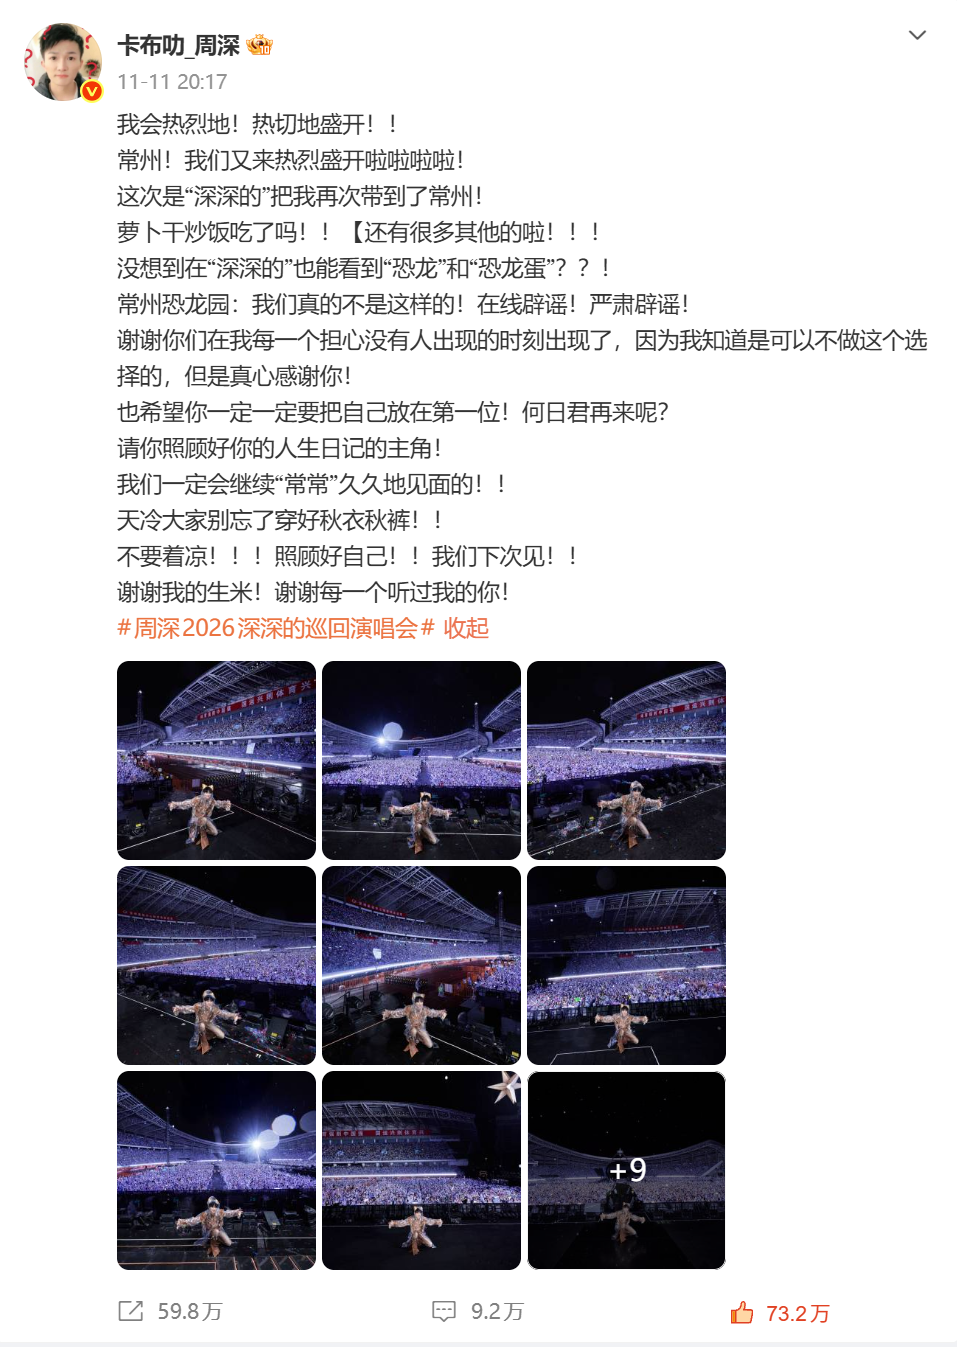
\includegraphics[width=280pt]{img/weibo/ChangZhou} 

}

\caption{周深2026.11.08常州场微博}\label{fig:unnamed-chunk-61}
\end{figure}

\chapter{2026.11.21厦门场}\label{XiaMen-20261121}

\begin{quote}
谢谢你们的出现，让非常普通的我成为了歌手周深，拥有了自己第100场演唱会，这是你们为我创造的奇迹。------周深
\end{quote}

\begin{figure}

{\centering 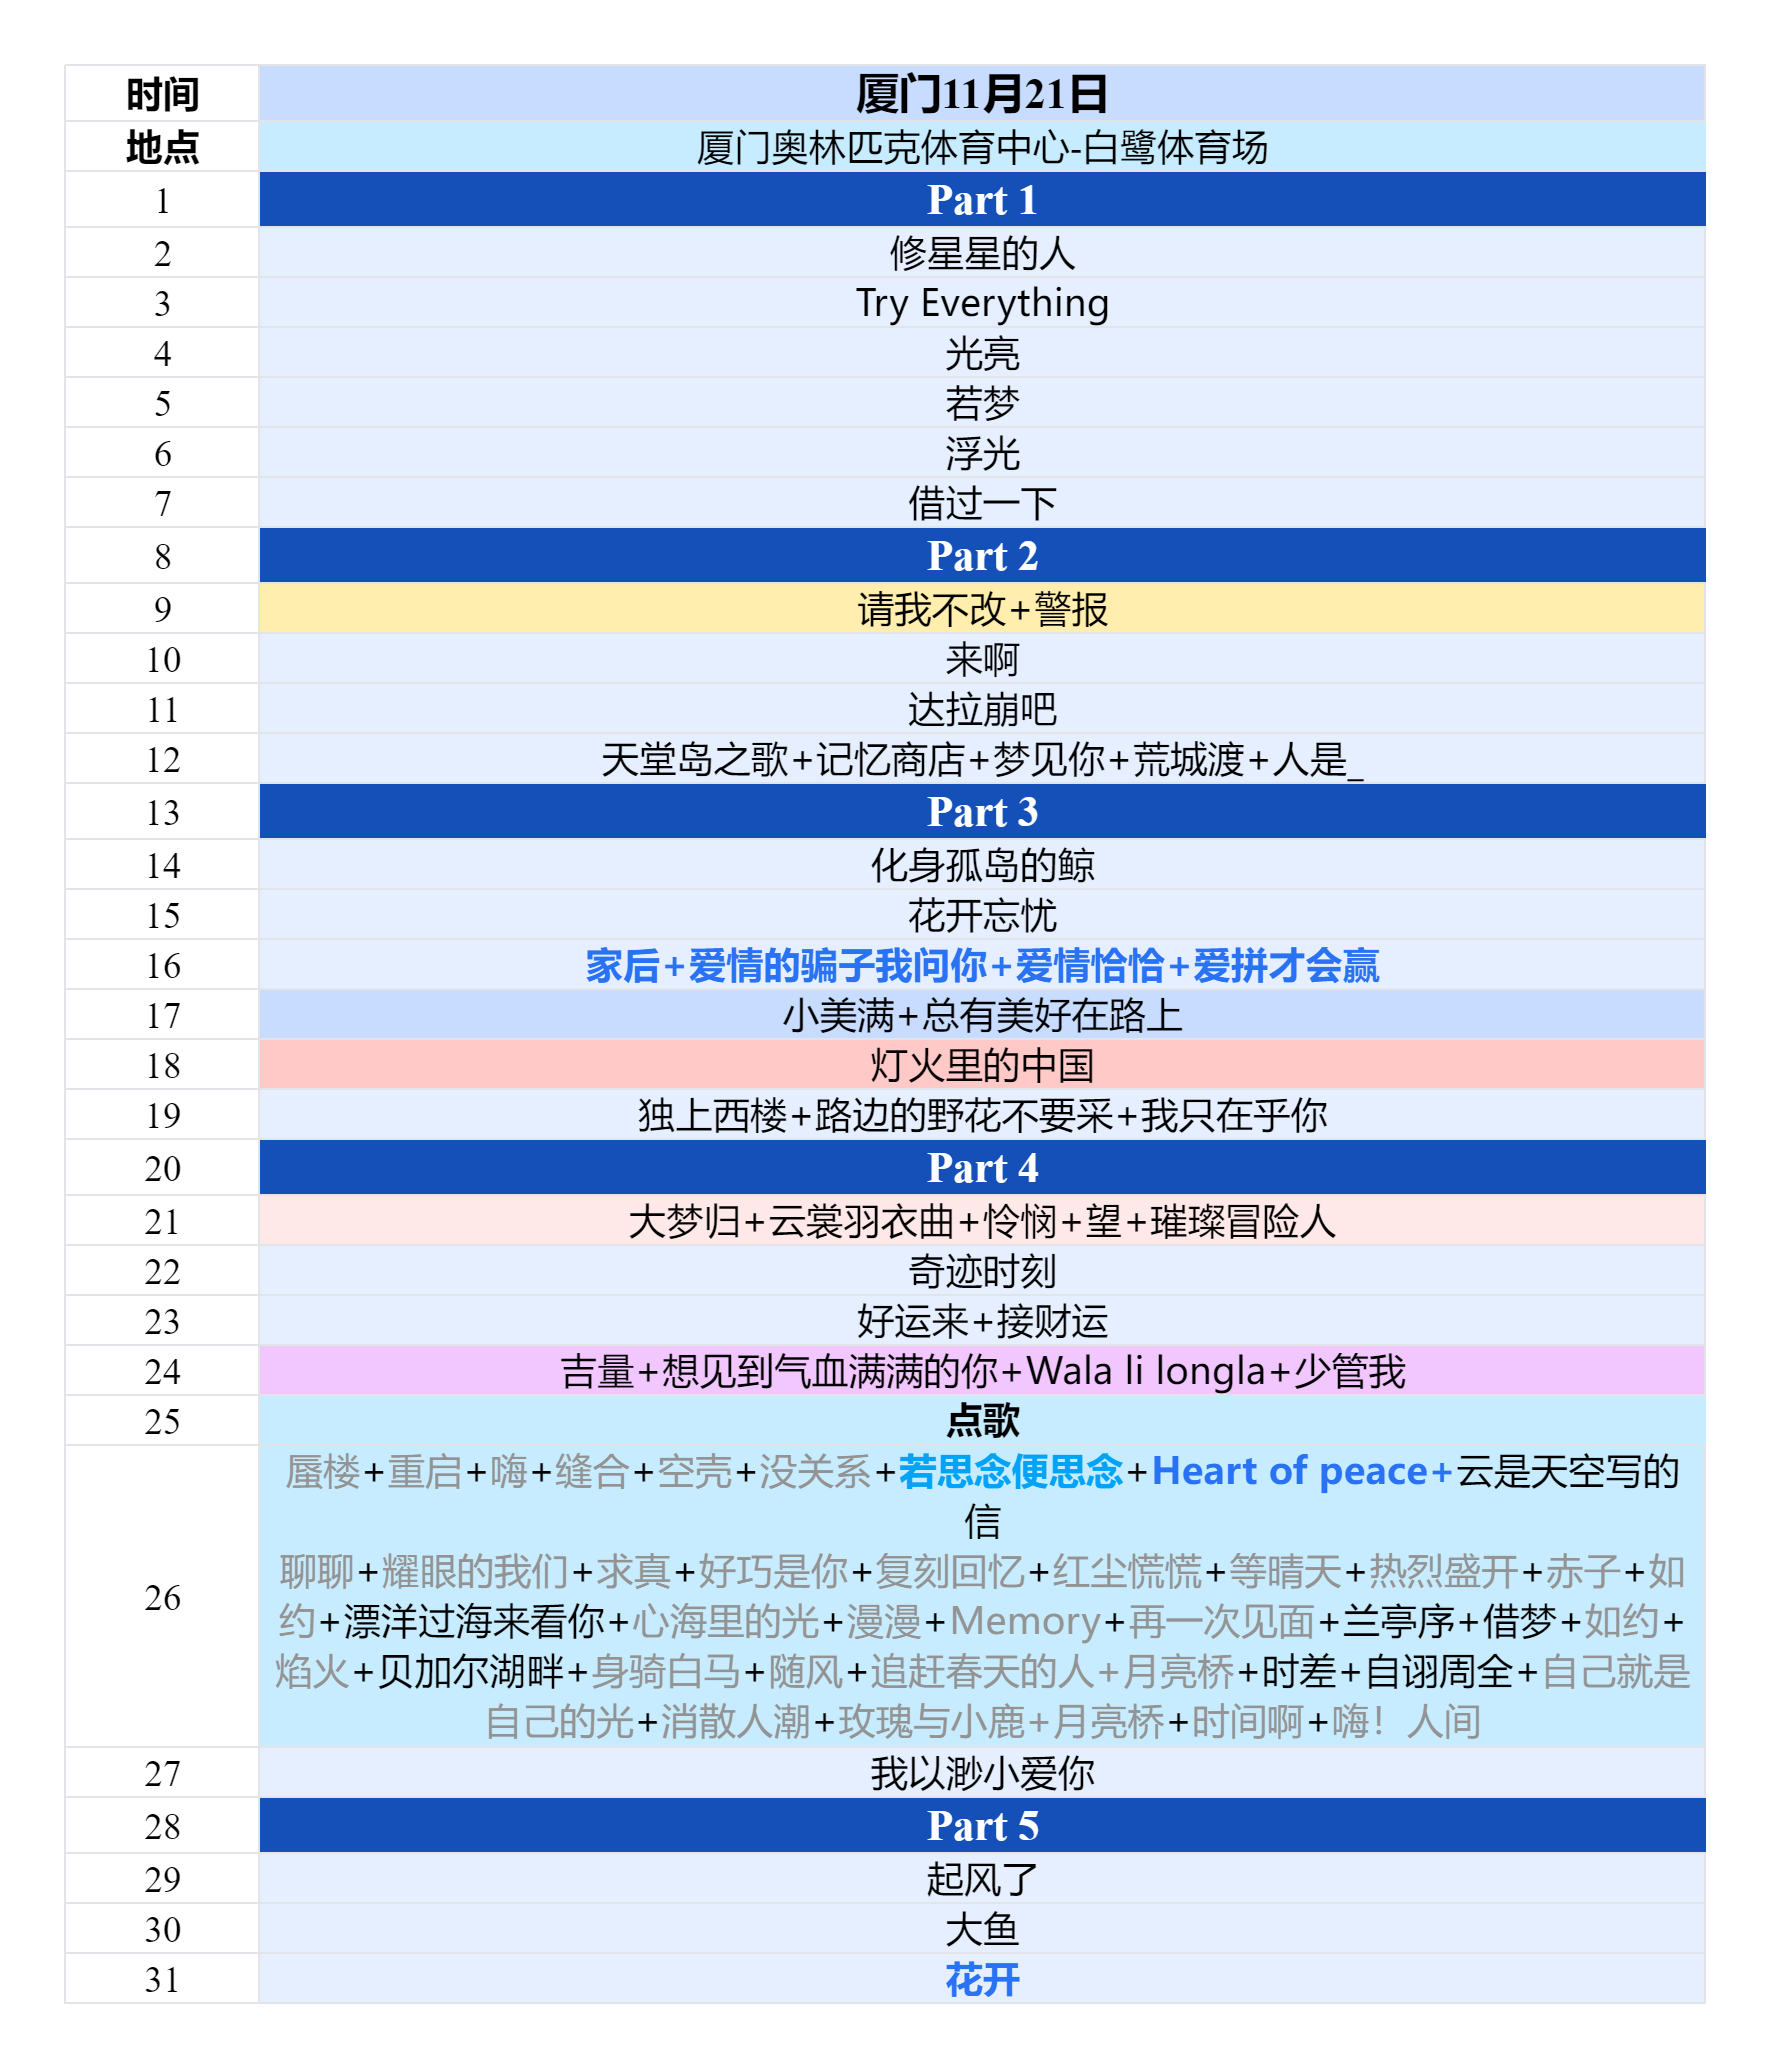
\includegraphics[width=280pt]{img/playlists/XiaMen-20261121} 

}

\caption{2026周深“深深的”巡回演唱会2026.11.21厦门场歌单（第100场）}\label{fig:unnamed-chunk-63}
\end{figure}

\newpage

\section{Part1}\label{XiaMen-20261121-part1}

\hyperref[opening-vcr]{🎥【\textbf{开场VCR}】}（VCR 正文见附录 D。VCR 结束后直接开唱。）

\hyperref[xiu-xing-xing-de-ren]{🎵【\textbf{修星星的人}】}（深：既然这宇宙让我诞生，想必它是要以我为证。我的情感和三十六度的体温，足以暖热即将熄灭的恒星）。厦门的朋友们你们好吗？（米：好------！）（欢呼）（尖叫）让我听到你们的尖叫声！（米：啊------！）（深：在时间的深海里，给地球道一声晚安）。

\hyperref[try-everything]{🎵【\textbf{Try Everything}】}既然这宇宙让我们诞生了，我们就勇敢地Try Everything好不好？（米：好！）周深第100场演唱会的观众你们好吗？（米：欢呼/尖叫）。尖叫声，（米：啊啊）。到你们，大声唱（米：Try everything）（和声：Oh oh oh oh）厦门的朋友（米：Try everything）（和声：Oh oh oh oh）（米：Try everything）。

  亲爱的朋友们你们好吗？我们又见面啦！（米：好------！）哇，居然在厦门看到我的朋友们穿毛衣。（米：欢呼/笑声）那我就放心了。厦门，上一次来的时候我还是被厦门烫到了，这次彩排的时候被冷到了。所以大家要记得添加衣物好不好？（米：好------！）这边的朋友你们好吗？（米：好------！）这边的朋友，后面的朋友你们好吗？（米：好------！）这边的朋友你们好吗？（米：好------！）来到厦门，我们闽南语肯定要说几句的。哎，说得不标准那就用唱啊。呃，稍等啊。大家好，我是周深。〔闽南语问候〕欢迎大家来我的演唱会。（欢呼）你们知道厦门最好吃的是什么吗？沙茶面。有吃吗？（米：有------！）竹笋冻。有吃吗？（米：有------！）哦，我发现厦门还有一个非常好吃的绿豆饼你们知道吗？因为只要你在地铁上你就会听到，``请对动饼，请门落车，落车请注意安全''。〔闽南语报站〕（欢呼/笑声）就厦门的朋友知道是什么意思。就是，哎好像是说车门它会开在左边对吧，然后从左边下车，下车要注意安全。但是我们外地的朋友听起来就感觉像是''掐''。（笑声）所以厦门的朋友们你们好吗？（米：好------！）谢谢你们，无论在任何时候都愿意成为我的光亮，也一定要记得好好的光亮你自己，好不好？（米：好------！）

\hyperref[silver-linings]{🎵【\textbf{光亮}】}你们好！（深：海上一阵风吹起，白云涌向陆地，季风带走沙粒\ldots\ldots 可是啊我却，愿意去相信）到你们。（深：可是啊，我却，米：却愿意相信，最渺小最微弱最柔软最无畏的你）厦门的朋友大声唱！（深：用尽了全力，努力地去回应，再无边再无尽再无解总有一线生机，光亮你自己，我爱你）。谢谢你们的出现，后面的朋友，谢谢你。

\hyperref[like-a-dream]{🎵【\textbf{若梦}】}跟你相遇这件事情，美好的就像做一场梦一样。厦门的朋友，我们一起唱这首《若梦》，好不好？（米：好------！）（深：浮生若梦，为欢几何\ldots\ldots）最大声！（米：往事流转，在你眼眸）（深：一边遗忘，米：一边拼凑！）（米：如我虔诚，合十双手）怎么了（米：唯愿你能，得到拯救）谢谢你的出现。因为你的出现，周深得到拯救啦！（米：欢呼/尖叫）再大声！（米：往事流转，在你眼眸。）好好听，（米：一边遗忘，一边拼凑。深：如我虔诚，合十双手。唯愿你能，得到拯救）全场最大声！(米：往事流转在你眼眸)(深【和声】：在你眼眸\textasciitilde\textasciitilde\textasciitilde)(米：一边遗忘，一边拼凑)(深【和声】：一边拼凑\textasciitilde\textasciitilde\textasciitilde)(米：如我虔诚合十双手)(深【和声】：合十双手\textasciitilde)(深、米：唯愿你能得到拯救)。到你们。（深：唯愿你能，米：得到拯救）（深：因为\ldots\ldots 厦门的你你\ldots\ldots 你你们，周深才得到拯救------）。

\hyperref[floating-light]{🎵【\textbf{浮光}】}人生不过三万天，因为遇见了你，每一天都值得留念。一定要知道，你的存在非常重要。好不好？（米：好------！）到你们！（米：浮光掠影重山彩云间）最大声！（米：你的伏线穿越千百年）最大声！

\hyperref[excuse-me]{🎵【\textbf{借过一下}】}（深：潇洒不是不怕，是愿付出代价）你还愿意吗？（米：愿意！）（深：谢过赐教的话，路借过一下）厦门的朋友你们好吗！（欢呼/尖叫）让我们唱，（深：让我大醉一场），唱！（米：殿堂之上，背闲诗两三章）再大声！(深、米：让我穿白衣裳，米：过疯人巷，去泥潭捞月光，深、米：望大人们见谅)。再大声（米：话谢过，路借过，你是你，我是我）全场（米：话谢过，路借过，你是你，我是我）。你们就是我要找的月光，我找到你们啦！（米：欢呼/尖叫）。

\section{Part2}\label{XiaMen-20261121-part2}

\hyperref[robot-vcr]{🎥【\textbf{机器人VCR}】}

\hyperref[brave-heart]{🎵【\textbf{请我不改}】}深：宝你个头！厦门的朋友们，让我听到你们最大声的尖叫声！（米：欢呼/尖叫）（深：是谁不断日夜合围，向我追来，痛击我最脆弱短板\ldots\ldots）尖叫声。全场（深：Brave heart）到你们（米：Brave heart！）（深：Brave heart）（米：Brave heart！）。
\hyperref[jing-bao]{🎵【\textbf{警报}】}（深：我发送警报声，血红色惊叹号，提醒你自救。被遥控，被耗空，快失控，快断送\ldots\ldots）。尖叫声！（米：尖叫）

  酷不酷？（米：酷）这么酷的一首歌，最后是用来唱错歌词。坦荡痛快！谢谢你们。那如果下一次还要邀请你们来深深的巡演，你们还愿意来吗？（米：愿意------！）问这句话是为了串下一首歌。这首歌的名字叫做《来啊》，需要你们配合跟我一起唱好不好？就有一段，如果没有听过的朋友，我们现场学一下。就是我唱''Don't tell me''，你们就唱------来啊啊啊啊啊，来啊啊啊啊啊！好不好？（米：好------）（深：Don't tell me）（米：来啊啊啊啊啊，来啊啊啊啊啊）哦，诶，后面的朋友唱大声点。（深：Don't tell me）（米：来啊啊啊啊啊，来啊啊啊啊啊）再大声点。（深：Don't tell me）（米：来啊啊啊啊啊，来啊啊啊啊啊）哎呦很厉害耶，学得很快哦。再来一遍哦，复习一遍。（深：Don't tell me）（米：来------）这首歌就靠你们了哟，求求你们了好不好？（米：好------！）那就，来呀！（欢呼/尖叫）

\hyperref[lai-a]{🎵【\textbf{来啊}】}来喽（深：Don't tell me，米：lie eeee，Lie eeee，我望眼欲穿你别闪躲）再来（深：Don't tell me，米：lie eeee，Lie eeee）。\textbf{\textcolor{red}{我爱你们}}！再大声。（深：Don't tell me lie eeee\ldots\ldots 敢不敢直视我，Let's fall）。

  接下来到了我们深深的巡回演唱会的小游戏环节喽。每个人可以自行在五秒内选择你喜欢的颜色，我们的荧光棒可以自己换颜色哦，分别是黄色、蓝色、粉色和绿色，请注意没有红色这个选择，大家不要按错喽。五、四、三、二、一，大家换好了吗？不同的颜色代表你选择了不同的角色，蓝色代表的是达拉崩吧，黄色代表的是国王陛下，粉色代表的是公主米娅，绿色代表的是恶龙。怎么会有那么多红色？怎么会每一场演唱会都要问这个问题？红色，让我想一想啊，先\ldots\ldots 先你就红色吧。不同的角色都有他们相对应的台词，那就是，当我喊到你们的时候，你们喊出对应的台词好不好？（米：好------！）这么冷的厦门还能出汗。那就是，达拉崩吧！（米：我最棒！）国王陛下！（米：再说一次！）公主米娅！（米：救我啊！）恶龙！（米：啊呜！）啊呜啊呜对不对？好。红色的朋友，高喊，厦门！（米：宝贝！）不要嘛，是不是啦，好不好？完全没人配合是吗？那，厦门！（米：宝贝！）好孤单啊。厦门！（米：宝贝！）达拉崩吧！（米：我最棒！）国王陛下！（米：再说一次！）公主米娅！（米：救我啊！）恶龙！（米：啊呜！）恶龙！（米：啊呜！）达拉崩吧！（米：我最棒！）国王陛下！（米：再说一次！）公主米娅！（米：救我啊！）恶龙！（米：啊呜！）厦门！（米：宝贝！）厦门！（米：宝贝！）（欢呼）哎。恶龙乘以十，走！（米：啊呜！啊呜！啊呜！啊呜！啊呜！啊呜！啊呜！啊呜！啊呜！啊呜！）今天这是第一百场。我们的恶龙不会要乘以一百吧？这个单你们接不接？（米：接！！！）这个也接，我不敢接。那我们一起来回顾一下这个童话故事吧。恶------龙------（米：啊呜！啊呜!）

\hyperref[dalabengba]{🎵【\textbf{达拉崩吧}】}（深：很久很久以前，巨龙突然出现，带来灾难，带走了公主又消失不见\ldots\ldots）全场，达拉崩吧！（米：我最棒！）国王陛下！（米：再说一次！）公主米娅！（米：救我啊！）恶龙！（米：啊呜！）达拉崩吧！（米：我最棒！）达拉崩吧！（米：我最棒！）厦门！（米：宝贝！）恶龙！（米：啊呜！）（米/深：达拉崩吧斑得贝迪卜多比鲁翁）（深：砍向------）（米：昆图库塔卡提考特苏瓦西拉松）（深：然后------）（米：昆图库塔卡提考特苏瓦西拉松）（深：咬了------）（米：达拉崩吧斑得贝迪卜多比鲁翁）（深：最后，达拉崩吧斑得贝迪卜多比鲁翁，战胜了，昆图库塔卡提考特苏瓦西拉松，救出了公主米娅莫拉苏娜丹妮谢莉红，回到了蒙达鲁克硫斯伯古比奇巴勒城\ldots\ldots）达拉崩吧的全名是？（米：达拉崩吧斑得贝迪卜多比鲁翁！）打败了？（米：昆图库塔卡提考特苏瓦西拉松！）厦门！（米：宝贝！）我被你们打败了。达拉崩吧的全名是？（米：达拉崩吧斑得贝迪卜多比鲁翁！）阿木的全名是？有人认识阿木吗？他只是一个导演，我配音的那个角色，他的全名我也不记得了。达拉崩吧全名是！（米：达拉崩吧斑得贝迪卜多比鲁翁！）哇，很厉害哦！尖叫声！（欢呼/尖叫）。谢谢你们。（米：谢谢周深）

  哇，太开心了，谢谢你们的出现。哇，我真的不敢想今天居然是自己的第100场演唱会。我演过台下只有三个观众的演出，也演过五个，也演过一百个都不到的，然后再到后面能够到Livehouse，再到剧场，再到体育馆，再到体育场。谢谢每一个听到我、看到我、向我投向善意的你，谢谢你们！（米：谢谢周深！）到了100场，我们应该更加的明白每一场都是非常重要的回忆啊，非常重要的一步，就像每一个你都是非常非常重要的存在。谢谢你们的出现，让一个非常普通的人成为了歌手周深，谢谢你们！（米：谢谢周深！）在前年，我发了第二张专辑叫做《反深代词》。这张专辑说的是200年的世界，这个世界叫做反深代词，一共有12个不同的情绪碎片，也就是周深化身成了12个不同的情绪碎片融合在这张专辑里。你发现某首歌跟你的经历、跟你的那个感情完全一模一样同频的话，那证明了我们在200年的世界彼此相互拥抱，我们彼此认出彼此啦。所以求求你们去听一下这张专辑好不好？（米：好！）线上也可以听哦，因为诶，它的实体也发行啦。还有朋友还在等吗？（米：没有！）大家都拿到了是吗？（米：是！）哇，你们有听懂里面的故事吗？（米：有！）有对不对？我们在线上也可以看到每首歌都有个故事。那在《反深代词》里面的蜃楼，接下来又发生了一些什么样的故事呢？我们一起去看看吧。

\hyperref[haven-song]{🎵【\textbf{天堂岛之歌}】}（深：宝你们个头\ldots\ldots 宝你们个头\ldots\ldots 宝你们个头\ldots\ldots）（深：叮咚，我有一个秘密，悄悄告诉你，欢迎你来到天堂入口\ldots\ldots）生米们，你们在哪？（米：在这里！）听过周深唱歌的你在哪里？（米：在这里！）
\hyperref[the-memory-store]{🎵【\textbf{记忆商店}】}诶，这是哪里？哦，这是深深的巡回演唱会对不对？（米：对！）我们在的城市是------（米：厦门！）哎，有点不一样。我梦到过这样的场景，那个时候他们做了美甲。有人只涂了一只。今天\ldots\ldots 好像没有这么冷啊。哦我知道了，这是《反深代词》里的记忆商店。在这里只要通过我们这一颗米子心，就可以唤醒我们最喜欢的那段回忆。哦\ldots\ldots 我盲猜，你没有做美甲。让我把手套摘下来，可以吗？猜中了！那让我们来看一下这一段回忆好不好？（米：好！）
\hyperref[meng-jian-ni]{🎵【\textbf{梦见你}】}（深：看着眼前，还年少的你，恍如流年从未淌过去\ldots\ldots 与你重逢在另一场梦境，但愿那时你在人海里，仍将我一眼认清）。你是一个坏竹荪。哦，因为我们这是周深第几场演唱会呀？（米：一百场！）三个都要捏爆吗？只捏这两个？大家要看到三个都捏爆好不好？（米：好！）开始吧。嗯？你也要负责一个哟。好的来，三二一。哇，哇这个爆出来的效果好差啊。这是我的麦克风诶。
\hyperref[huang-cheng-du]{🎵【\textbf{荒城渡}】}（深：夜色中寻觅过，当往事困住我，也盼心中生出一点萤火\ldots\ldots 眼中拂尘，手中残魂，那故事斑驳荒城\ldots\ldots 握一颗糖暖这孤身）。
\hyperref[Humans_are_]{🎵【\textbf{人是\_}】}（深：未知摊开棋局，舍弃昨日才可破\ldots\ldots）全场帮我一起唱！(深：让时空消亡我)(米：你无需记得我)(深：来摧毁我深爱的一切，可仍夺不走我的选择)再大声！（深：弹指间湮灭我）大声唱，（米：但命运打不败活着）（深：是微茫中高歌的族类，生命像烟火那就点亮，孩童的双眸）。到你们唱（米：未来的瞳孔。）（深：未来的瞳孔）。

  在遇到你们之前，我也认为那些失去的、过去的是最好的。但是听到了你们的唱歌，This is true music，让我明白，我们现在相遇的每一分每一秒，才是最值得珍惜的。我们都不要被困在记忆商店里，你们说对吗？（米：对！！！）是你们创造了不朽的永恒的爱，谢谢你们出现！

\section{Part3}\label{XiaMen-20261121-part3}

\hyperref[music-animations-vcr]{🎥【\textbf{音乐动画VCR}】}

\hyperref[The-whale-who-became-an-island]{🎵【\textbf{化身孤岛的鲸}】}你们好吗？（米：好）（深：我是只化身孤岛的蓝鲸，有着最巨大的身影\ldots\ldots）（深：我爱地中海的天晴）（米：爱西伯利亚的雪景，爱万丈高空的鹰，爱肚皮下的藻荇，我在尽心尽力地多情，直到那一天）。（深：我的背脊如荒丘，而你却微笑摆首，把它当成整个宇宙）。（深：我想给你能奔跑的岸头）（米：没有墙头）最适合带着哭腔唱的一句出现了。（深：你们究竟有多少个墙头？）（米：没有！）诶，很多人不知道''墙头''是什么意思。就是当我在问生米，诶，你们喜欢哪个歌手啊？他们会说------（米：周深！）然后我就会问呐，你们除了周深还喜欢哪些歌手啊？（米：没有！）他们就会骗我说没有。我呢就非常的不礼貌，哎呀我也确实挺不礼貌的，就把他们喜欢的其他歌手称为''墙头''。所以就会问他们，（深：你们究竟有多少个墙头？）（米：没有！）但无论如何，叫你们好好的照顾好自己。（深：你们就是我的国王和王后）。

\hyperref[Blossoms-that-forget-sorrow]{🎵【\textbf{花开忘忧}】}厦门的朋友你们好吗？（米：好！）我们来厦门看你咯！（深：忘忧草\ldots\ldots）好，我们重新来一下这首歌。不可接受。厦门的朋友你们好吗？（米：好！）我们来厦门看你们咯！后面的朋友！你们来第一句。（深：巷子口）（米：买了花，穿过沿街红墙青瓦）。（深：若记忆被偷走了，忘了我的爱，我会说）说什么？（米：你好啊！）你们好吗？（米：好！）（深：这是给你的花，花的名字叫忘忧草，它说时光汹涌如水上烟波，别走远了，一起回家）我们一起回家好不好？（米：好！）我们一起！（深、米：我们苍老的时候就回到小时候，采青梅用来酿酒你不许偷着喝，穿朴素的衣裳牵着那衣袖，捡了小猫名为苍狗）到你们！（米：我们睡去的时候像孩子无忧愁，反正也很难上锁）。（深：忘忧草开着花，你在月光下不说话，一件遗憾的事就喝一杯茶，庭院深深，秋叶飘落）。

  在我们的人生当中，一定有那样一个非常非常重要的人，也住着一份遗憾，可能再也没有机会见到他了。但是我相信，只要我们的思念越大声，他就一定听得到。你们说对吗？（米：对！）所以我们一定要好好的照顾好自己，因为他也一定感受得到。你们说对吗？（米：对！）花开忘忧，愿你无忧。花开忘忧！（米：愿你无忧！）谢谢你们！（米：谢谢周深！）

  哇，好开心来到厦门开演唱会。因为就会有很多很多非常好听的闽南语的歌曲。（欢呼）如果等一下你会唱，跟我们一起唱好不好？（米：好！）大家都知道我的歌迷叫什么名字？（米：生米！）大家也不一定都知道。介绍一下，我的歌迷他们叫''生米''。然后还有一种非常非常好吃的大米叫五常大米。那你们知道厦门有一种非常好吃的米叫什么吗？叫''公虾米''！（欢呼/笑声）周深，你在公虾米（讲什么）。那等一下如果你会唱，跟我一起大声唱好不好？（米：好！）

🎵【\textbf{闽南语金曲串烧}】

\hyperref[jia-hou]{🎵【\textbf{家后}】}

\hyperref[ai-qing-de-pian-zi-wo-wen-ni]{🎵【\textbf{爱情的骗子我问你}】}（深：讲什么，我亲像天顶的仙女\ldots\ldots）提问（深：啊～我问你，啊～我问你，你的良心到底在，你的良心到底在，你的良心到底在哪里）欸，说到qia，大家还记得刚才说的，我们在地铁上经常听的那一段吗？qia在左边，qia门打开，下qia请注意安全。那还有一种qia，也很好听，叫爱情恰恰！（米：欢呼/尖叫）

\hyperref[ai-qing-qia-qia]{🎵【\textbf{爱情恰恰}】}荧光棒 （深：\ldots\ldots 爱情的恰恰\ldots\ldots 可惜身边的人，不是不是不是你）

\hyperref[ai-pin-cai-hui-ying]{🎵【\textbf{爱拼才会赢}】}大声合唱这首歌好不好？（米：好------！）你们会唱吗？（米：会）各位来宾，请大声的一起唱好吗？（米：好------！）（深：一时失志不免怨叹，一时落魄不免胆寒。哪怕失去希望，每日醉茫茫，无魂有体亲像稻草人。人生可比是海上的波浪，有时起，有时落。）到你们（米：好运，歹运，深：总嘛要照起工来行）大声唱！（米：三分天注定），诶 ？（米：七分靠打拼）最大声！（米：爱拼才会赢！）各位来宾，第二遍可以更大声一点吗？（米：可以------！）最大声！大声唱！大声点！\ldots\ldots 大声唱！（米：好运，歹运，深：总嘛要照起工来行）全场最大声！（米：三分天注定）怎么了？（米：七分靠打拼）再来！（米：爱拼才会赢！）（深：三分天注定）怎么了？（米：七分靠打拼）（深：爱拼才会赢！爱拼，米：才会赢！深：才会赢！）

\hyperref[simple-bliss]{🎵【\textbf{小美满}】}这首也要一起大声唱哦！（欢呼/尖叫）（深：没什么大愿望），唱，（米：没有什么事要赶）\ldots\ldots（深：乌云还挺大胆），怎么了？（米：顶在头上吹不散，深：我抓在手里捏成棉花糖，什么烦恼不能忘）\ldots\ldots 大家一起唱（深：你看小狗在叫，树叶会笑，风声在呢喃\ldots\ldots）谢谢你们！（米：谢谢周深）（深：笑一笑就灿烂）唱。大声唱！（深：你看小狗在叫，树叶会笑，风声在呢喃）唱！

  遇到你们就是我人生当中最美最美的美满！让我们一起在《小美满》这首歌当中许愿吧。我来打个样哦，像我这样闭上眼睛，想好心中的愿望。我会倒数，三、二、一，喊你睁开眼睛，我们的愿望就会出现在这棵许愿树上。现场无论什么年龄段，无论什么职业的朋友，闭上眼睛，想一想想要许的愿望。请相信相信的力量，请相信美好的力量。闭上眼睛许愿喽！想想生日的时候第一个蹦出来的愿望是什么呢？哦对了，在《小美满》这首歌当中的愿望，只能够许关于自己的愿望。想一想，是不是很久很久没有看见自己了？是不是很久很久没有拥抱过自己的委屈？是不是很久很久没有跟自己说一声，你做的真的很好，你真的很棒。想一想，是不是忘了跟自己说一句，我喜欢你呢？三、二、一，睁开眼睛！（深：你愿相信什么就把世界看成什么样，偶尔难题加点重量，越要轻轻地旋转。\ldots\ldots 笑就好，哭也好，今天就是明天最好的陪伴）到你们了！（深：笑就好，哭也好），你们（米：今天就是明天最好的陪伴）（深：你们都是周深最好的陪伴！）谢谢你们！（米：谢谢周深！）

  我其实是一个不爱过生日的人，但是因为你们的出现我发现，诶，9月29日这一天好像也挺特殊的哦。那也是因为你们的出现，我发现每一天都特别特别的特别。所以让我们祝今天生日的朋友\ldots\ldots（米：生日快乐！）你们真好。让我们祝昨天或者前一段时间过生日的朋友\ldots\ldots（米：生日快乐！）让我们祝明天或者过一段时间再过生日的朋友\ldots\ldots（米：生日快乐！）谢谢你们。因为你们呐，我看见\ldots\ldots{}

\hyperref[zong-you-mei-hao-zai-lu-shang]{🎵【\textbf{总有美好在路上}】}（深：花在开，云在飘，笑容在脸上）妞们（米：我们向前方，一路向阳）亲爱的你们（深：亲爱的你，米：在路上慢慢逛，看一看太阳）（深：让风轻轻）（米：吹拂你的脸庞）（深：今天过去，要到明天看看天气会怎样。阴或晴朗，故事都慢慢赏。抬头发现，你们就是光芒）（欢呼/尖叫）。

\hyperref[deng-huo-li-de-zhong-guo]{🎵【\textbf{灯火里的中国}】}灯火里的中国，美不美丽？（米：美！）也是由你们组成的哟！（深：都市的街巷已灯影婆娑\ldots\ldots 归港的船帆从灯塔掠过，追梦脚步月下交错\ldots\ldots）等一下我们一起大声唱这首歌好不好？（米：好------！）大声唱！（米：灯火里的中国，青春婀娜）再大声！（米：灯火里的中国，胸怀辽阔。深：灯火灿烂的中国梦）大声唱！（米：灯火荡漾着心中的歌）最大声！（深：灯火里的中国，青春婀娜）唱！后面的朋友！（米：灯火里的中国，胸怀辽阔。深：灯火灿烂的中国梦，米：灯火荡漾着心中的歌）（深：灯火荡漾着心中，米：的歌，深：的歌）。

  哎，现在怎么每次唱完歌就剩下你一位声乐老师在台上？他们都不愿意接受高音挑战对不对？你想，翔克老师想要接受，但是这个高音挑战是为你准备的。试一下好不好？不要再退了。准备好了吗？你想要接受高音挑战还是给大家说一个冷笑话？有热一点的笑话吗？（摄影师：笑话好了。）啊哦，好，来咯。（摄影师：呃，这个笑话是需要大家生米老师们一起帮我。）那还有其他不是生米的老师就不用帮你了吗？（摄影师：变魔术啊。）你还有魔术？魔术是什么可以很快就会学会的东西吗？尽量不会太长对不对？试一下啊，什么魔术？（摄影师：要生米老师帮我一起变个魔术。）哦，你们愿意帮他吗？（米：愿意------！）可以可以，来吧，你变吧。魔术要用机器吗？不用。来吧，你的魔术是？（摄影师：生米老师们帮我倒数三个数字。）哦，我们帮他倒数三个数字好不好？好了，准备好，你\ldots\ldots 不会又是什么烂梗吧？好害怕哦，你也``中虾？啊。来咯，三！（米：二！一！）变\ldots\ldots 变完了？这个魔术是？（摄影师：我们变得更喜欢你了。）（米：欢呼/尖叫）你在``做虾''啊。你在讲``虾米''啊？呃\ldots\ldots 受不了。那只能大家再唱一段歌来，来让我稍微舒畅一点点。（深：灯火里的中国，米：青春婀娜，深：灯火里的中国，米：胸怀辽阔。深：灯火灿烂的万里山河，米：初心换回了百年承诺）哇，你们（唱得）好好听啊，再来，（深：灯火里的中国，米：青春婀娜，深：灯，米：火里的中国胸怀辽阔。）大声唱（米：灯火灿烂的中国梦，灯火荡漾着心中的歌，深：灯火荡漾着心中的歌，\textbf{\textcolor{red}{我会变得爱你更多！}}）哎，你这个魔术我怎么没有学啊？我看一眼。真的有点被吓到，这位老师。

🎵【\textbf{邓丽君组曲}】
  好，我一直想要成为一个什么样的歌手呢？我希望自己可以成为像我的偶像这样的歌手，邓丽君女士一样。有好多好多歌，然后好多好多歌都存放着你们的故事，你们的回忆。所以我会继续好好唱歌，加油唱歌的。那你也要好好的为自己创造更多回忆和创造更多奇迹，好吗？（米：好！）如果遇到你会唱的歌，跟我一起大声唱好不好？（米：好！）

\hyperref[du-shang-xi-lou]{🎵【\textbf{独上西楼}】}（深：无言独上西楼，月如钩，寂寞梧桐，深院锁清秋，剪不断，理还乱，是你们的墙头）（米：没有）（深：还在这里说没有）（米：没有）那我们来对一下暗号，厦门------（米：宝贝！）（深：宝你个头）。

\hyperref[donot-pick-the-roadside-flowers]{🎵【\textbf{路边的野花不要采}】}这首会唱吗？（米：会！）大声，跟我一起唱，走！（深：送你送到，米：小村外，有句话儿要交代。深：虽说已经是百花开，路边的野花）它怎么啦？（米：你不要采！）最大声！（深：记着我的情，记着我的爱，记着有我天天在等待）再大声（米：我在等着你回来。深：千万不要把我来忘怀，千万不要把我来忘怀，千万不要把我来忘怀）你们会忘了我吗？（米：不会！）

\hyperref[I-only-care-about-you]{🎵【\textbf{我只在乎你}】}我时常在想，如果没有遇到你们，我现在在做什么呢？我的人生日记会长什么样子呢？没有答案啊。（深：如果没有遇见你，我将会是在哪里？日子过得怎么样？人生是否要珍惜？）（米：也许认识某一人，过着平凡的日子，不知道会不会，也有爱情甜如蜜）后面的朋友！（深：任时光匆匆流去，我只在乎你）大声唱！（米：心甘情愿感染你的气息）（深：人生几何------）怎么啦？（米：能够得到知己！）（深：失去生命的力量也不可惜）所以呢？（米：所以我求求你，别让我离开你）（深：除了你，我不能感到一丝丝情意）全场最大声，（米：任时光匆匆流去，我只在乎你）谢谢你们，（米：心甘情愿感染你的气息）再大声！（深 ：人生几何，米：能够得到知己！深：失去生命的力量也不可惜，所以我求求你，别让我离开你，除了你，我不能感到一丝丝情意，除了你，我不能感到）什么？（米：一丝丝情意）（深：除了你，我不能感到一丝丝情意）谢谢你的出现，我！只！在！乎！你！（欢呼/尖叫）

\section{Part4}\label{XiaMen-20261121-part4}

\hyperref[mask-vcr]{🎥【\textbf{面具VCR}】}（VCR：你说，对吗？）（米：对！！！）（VCR：我没听到哦，你们说，对吗？）（米：对！！！）你们愿意跟我一起唱吗？（米：愿意！！！）

\hyperref[da-meng-gui]{🎵【\textbf{大梦归}】}（深：春尽枝头慌，再一季，花开无人赏，再一句，感人间万般皆寻常\ldots\ldots 大梦终不归）你们会唱吗？（米：会！）一起哦。（深、米：就让冷风吹）（米：雨纷飞，留一地伤悲）（深、米：就让爱破碎）（米：恨成灰，往事都作废）（深、米：就让火一堆，酒一杯）（米：送一袖清晖）（深、米：就让因后退，果上追，大梦终不归）。

\hyperref[Song-of-the-cloud-dress]{🎵【\textbf{云裳羽衣曲}】}我们的缘分一定不会太浅，因为我的名字叫------（米：周深！）我们巡演的名字叫------（米：深深的！）大声唱给我听好不好？（深：故事鲜艳，米：而缘分却太浅，深：我的爱恋，竟如此的明显，我不停地默念，想牢记你的容颜）再大声！（深：故事鲜艳，米：而结局却搁浅，深：这些年你又在那座红尘之间，幻化成哪张脸）。

\hyperref[lian-min]{🎵【\textbf{怜悯}】}（深：我要比你显得更无情，再生一场病）（米：怜悯是讨来的公平）（深：我要带着爱意恨着你，米：逢人就美化你罪行。深：我要抱着余烬守伶仃，蘸着真心，隔岁月惦念你）我们不要祈求怜悯，我们都值得被好好的爱着，对不对？（米：对！）

\hyperref[Expectation]{🎵【\textbf{望}】}所以无论你在哪儿，我们都会绕啊绕，绕回彼此身边。一起唱吧！（深：我们总会绕啊绕），唱，（米：绕啊绕，绕几千里路也望向归途）（深：乘着风，想念吹拂，有夜空漂浮，抓一颗流星做礼物，愿你幸福。手中线，绕啊绕，米：绕啊绕，深：绕几千日夜也望向归途，燕归巢，迁徙之路，参与者无数，待到烟火照夜白时准备庆祝，我们心有所住）。大声唱！（深：我们总会，米：绕啊绕，绕啊绕，绕几千里路也望向归途，深：乘着风，想念吹拂，有夜空漂浮，抓一颗流星做礼物，你要幸福。\ldots\ldots 我们心有所住）

\hyperref[adventurers]{🎵【\textbf{璀璨冒险人}】}璀璨冒险人们，你们准备好了吗？（米：好------！）我们一起继续出发吧好不好？（米：好------！）（深：他们说要越过前方风沙，必须低着头；他们说要绕过蜿蜒的河，才能往前走；他们说烫要放手，太远要换个路口；如果得不到谁的认同，那就不算拥有）到你们！（深：没人能够，米：决定谁的一生应该怎么活，深：没人能够，米：定义谁的天空是什么颜色；深：没人未梦就先懂，只是单纯相信着；背向光的英雄，每张轮廓出自平凡的沉默）你们就是我的英雄！（深：就让一路曲折，每一道伤口，洗净我的脆弱）全场一起！（深：原来咽回去的泪\ldots\ldots）到你们。（深：要炙热啊！要不忘啊！要勇往啊！起风了，呼唤了，你还在等什么？挥手了，再见了，别不舍回头啊。向心中的梦啊，去追吧。要能留下伤痕才算活过，愿你记得，愿你哭过，不惧脆弱，不惧脆弱，不惧脆弱）希望你永远不要害怕看到自己脆弱的一面。它也是组成最完美的我们的一部分。好不好？（米：好------！）希望你永远有那一颗无畏的心，赤诚的心。也同样（深：不惧脆弱）就像我变魔术那样不知脆弱，那怎么办呢？因为这就叫做奇迹时刻。

\hyperref[miracle-moment]{🎵【\textbf{奇迹时刻}】}荧光棒！（深：从银河抹去的恒星，穿梭时空的王牌，一个瞬息就能将不思议解开\ldots\ldots）你们准备好了吗？我要开始变魔术啦！（欢呼）你们准备好了吗？（米：准备好了！）我没准备好。掌声鼓励。（欢呼/尖叫）大家看啊，大家怎么看呢？这是一个非常普通的方块累积起来的一个塔，对不对？没有任何问题吧？现在红色在最上层，对不对？那等一下我就会用魔术把它变到另外一层。掌声在哪里？期不期待？（米：期待！）三、二、一！（欢呼/尖叫）你们不会以为这样就结束了吧？帮我倒数五个数字！五（米：四！三！二！一！）（欢呼/尖叫）厉不厉害？（米：厉害！）还有更厉害的，大家看，这是不是四张非常普通的扑克牌，对不对？（米：对！）好，这里有一个空白的画架，对不对？没有问题吧？（米：没有！）大家看没有问题对不对？那我们现在呢，就把这个空白的画架给它放在这里哦。好紧张。不要拍它，先不要拍它啊。你先不要这样看我。这里有个蓝色的颜料，对不对？（米：对！）那这种情况下呢，我们就是要把这个颜料全部挤进去，对不对？（米：对！）挤扁了。哎，那接下来还有一瓶绿色的颜料，对不对？也按照刚才一样的，我们直接就把它挤进去。挤完喽。还有一瓶红色的颜料，对不对？但是有一天因为我太开心了，因为跟大家见面了，所以就一不小心，哎呀，把它\ldots\ldots 把它踩碎了。那我们同样把它挤进去好不好？来给我倒数三个数字，来，三、二、一！因为你们呐，所有黑白的世界都变得彩色了哟。（欢呼/尖叫）（音效：礼炮声）迟来的特效声音非常的阴阳怪气，不知道为什么。

\hyperref[good-fortune-comes]{🎵【\textbf{好运来}】}那好运来了你们接不接？（米：接！！！）厦门的朋友，好运来了接不接？（米：接！！！）等一下大声的唱好不好？（深：叠个千纸鹤，再系个红飘带，愿善良的你们天天好运来\ldots\ldots 你凤舞太平年，你龙腾新时代，你幸福的家园迎来百花盛开）你们唱！（深：好运来祝你好运来），唱（米：好运带来了喜和爱）厦门的朋友大声接好运！（米：好运来我们好运来，迎着好运兴旺发达通四海）身体健康，接不接？（米：接！！！）恭喜发财，接不接？（米：接！！！）\ldots\ldots 厦门的朋友大声唱！唱！再大声！张嘴唱！（米：好运来祝你好运来\ldots\ldots）厦门的朋友好运来了接不接？（米：接！！！）

\hyperref[jie-cai-yun]{🎵【\textbf{接财运}】}那等一下，用你们最大的声音一起接所有最美好的事情好不好？（米：好！！！）我们一起，接平安！（米：接平安！）再来大声接，平安！（米：接平安！）来接幸福！（米：接幸福！）接健康！（米：接健康！）接财运！（米：接财运！）接不接？（米：接！！！）（深：接个好运来，接个福气来，接个财神开开心心到我家里来，接个财运来，小财大财，我接我接，我接金山银海）\ldots\ldots 祝厦门的朋友，恭喜发财，接不接？（米：接！！！）后面的朋友接不接？（米：接！！！）那我就要坐着我们的小车车来看一下，有谁没有好好的接好运的哟。祝大家依然在马年拥有无量的吉祥，接不接？（米：接！！！）

\hyperref[ji-liang]{🎵【\textbf{吉量}】}《吉量》这首歌你们会唱吗？（米：会！！！）哦试一下啊，（深：羲和车上金铃铛），你们？（米：叮当叮当\ldots\ldots）（欢呼）那等下也要一起大声唱好不好？（米：好！！！）那我们就载着无量的吉祥，出发喽！你们好！（米：好------！）（羲和车上金铃铛，叮当叮当）到你们（米：叮当，叮当）这边（望舒驾后银尾巴，深：摇摇晃晃）你们（米：摇摇晃晃）。（深：九天之上飘来一朵雪花），你们好！（深：原来是我的英俊的小马，金色星星在它眼里安家，祝融手持火种编织了它的发）你们好吗？（米：好------！）（深：我的小马一天一天长大，穿过凛冬和最沸腾的夏）你们好吗？（米：好------！）你们好吗？\ldots\ldots 全场！\ldots\ldots 全场！你们好吗！？

\hyperref[xiang-jian-dao-qi-xue-man-man-de-ni]{🎵【\textbf{想见到气血满满的你}】}上面的朋友你们好吗？看台的朋友，这边的朋友，请问（深：你是谁？你是自己的？）（米：宝贝！）（深：有时候感觉自己多珍贵）你是最珍贵的！（深：还会有更好的等着你，还有好多梦在飞，还要给自己一个新的机会）你（深：要早起早睡，别那么累，做好气血满满的准备。想见到你，灿烂的你，无惧也无畏。别害怕疼痛，别怕眼泪，就让我来陪着你找回，手里有暖，心里有暖，阳光的明媚）我爱你们！（深：有再冷再苦再痛的时候，请你一定记得，我永远会是你停靠的选择。）你们好吗（深：唯有梦可贵，勇气可贵，举起热情满满的奖杯，那时的你，灿烂的你，无惧也无畏）厦门的朋友你们好吗？（米：好）（深：你是谁？你是自己的------）（米：宝贝！）（深：你是自己的------）（米：宝贝！）谢谢你们。

\hyperref[wala-li-longla]{🎵【\textbf{Wala li longla}】}在我发的新专辑《反深代词》当中有一个快乐密码，等一下我们一起大声地喊出这个快乐密码，我们就会越来越开心好不好？（米：好------！）我教你们一下哦，Wala li longla！（米：Wala li longla！）我们看台的朋友，你们好吗？Wala li longla！（米：Wala li longla！）全场一起哦，Wala li longla！（米：Wala li longla！）（深：把蜗牛都放大，把汽泡堆成塔\ldots\ldots）你们好吗？你们好吗？（深：我看的永恒都是一刹那，虚拟与现实同等构架，Wala li longla，快乐最伟大）你们好吗？厦门的朋友，希望你跟我一起大声喊出这个快乐密码，我喊什么，你就喊什么，跟我一起好不好！（米：好！）来咯！Wala！（米：Wala！）Wala li！（米：Wala li！）Wala li long！（米：Wala li long！）Wala li longla！（米：Wala li longla！）这边的！Wala！（米：Wala！）Wala li！（米：Wala li！）Wala li long！（米：Wala li long！）Wala li longla！（米：Wala li longla！）大声！Wala！（米：Wala！）Wala li！（米：Wala li！）Wala li long！（米：Wala li long！）Wala li longla！（米：Wala li longla！）Wala！（米：Wala！）你们好吗？Wala li！（米：Wala li！）Wala li long！（米：Wala li long！）Wala li longla！（米：Wala li longla！）大声唱！（深：Wala li longla，快乐是悄悄心照不宣玩耍，心里有花吧\ldots\ldots 管他是奇葩还是没想法，快让梦发芽）。你们好吗？全场跟我最大声来一次！Wala li longla！（米：Wala li longla！）

\hyperref[watch-ur-manners]{🎵【\textbf{少管我}】}我们还有一个暗号哟，3、2、1，嘿，少管我！3、2、1，嘿！（米：少管我！）全场最大声，3、2、1，嘿！（米：少管我！）荧光棒，让我看到你！谢谢你们来跟我们见面！（深：有什么关系，删掉无聊的理由，把沉重身体传送到热带气候\ldots\ldots 做生活困兽，不如去浪漫宇宙）你们好吗？会场的一起。（深：我想我可以，抓住风中飘散的花，\ldots\ldots，或成为昆虫砂砾一片雪花）你们好吗？3、2、1，嘿！（米：少管我！）3、2、1，嘿！（米：少管我！）那边的朋友，3、2、1，嘿！（米：少管我！）这边的朋友，3、2、1，嘿！（米：少管我！）谢谢你们的出现！5、4、3、2、1，嘿！（米：少管我！）。

  厦门的朋友真的太棒了！给自己一点点掌声！（欢呼）哇！在厦门看到羽绒服了吗？好神奇。但是看到每一个人都非常的热情，非常的可爱，非常的\ldots\ldots 在我心中非常的完美、漂亮、帅气，我觉得真的真的很幸福。谢谢你们来跟我们见面。《少管我》是一首非常轻松活泼的歌，不是让你去争执，而是让你在寻找自己的路上如果听到一些杂音，在不打扰别人的前提下就轻轻松松说一句------嘿！（米：少管我！！！）做自己这件事情，没有人做得比你更好，好吗？（米：好！！！）那我们就一起来点歌吧！（欢呼）

【\textbf{点歌环节}】\\
  全场帮我倒数五个数字，五！（米：四！三！二！一！）停！您好。（小戴：周深好！宝贝！）（欢呼/笑声）宝你个头。请问怎么称呼您？（小戴：我叫小戴。）小戴。是来自哪里的朋友？（小戴：我来自福建泉州，然后现在在福州读书。）来自福建泉州的朋友在福州读书，然后我们在厦门见面。（小戴：对。）哦！大家欢迎我们的小戴！（欢呼）泉州也说，跟这边说一样的话吗？家乡话。不一样，一样？（小戴：不一样。有一些区别。）哪一些？你会唱这歌吗？（深用闽南语唱：讲什么，你亲像天顶的仙女）（小戴用闽南语接唱：讲什么，我亲像古早的西施）哦还是很像的哟。那用就是用你的家乡话跟我们打个招呼，就深深的巡回演唱会的朋友们大家好，欢迎大家来到深深的巡回演唱会。（小戴：要不你来教我吧，我只会前面这一句闽南话。）呃，我不会说闽南话。我只会说''打给厚，哇系纠清''。〔闽南语''大家好，我是周深''〕欢迎大家来我的演唱会。是不是？还可以哦。好了，你第一次听我的歌是哪首歌呀？（小戴：2021年的春晚《灯火里的中国》。）（欢呼）你记词还是不记词？我想让你给大家唱一段。记词还是不记词？歌词记得住吗？（小戴：我\ldots\ldots 我唱的没你好听，因为你是宝贝。）（欢呼/笑声）已经聊不过了。宝你个头。那我们就唱不记词的那段吧。（深演唱《灯火里的中国》高音吟唱片段：啊啊啊，小戴：啊啊啊，深：啊啊啊）好吧好吧。今天是一个人来的吗？（小戴：是。）哦一个人来的，谢谢你。那再给我们唱一句。（深：我身骑白马，小戴：走三关，深：我改换素衣，小戴：回中原）你是回湖南了吗？``喂，回湖南''。那帮我们点出今天第一首歌好不好，小戴？小戴情绪好稳定哦。（小戴：我想听一首英文歌。）（欢呼）厉害的哟。那在深深的巡回演唱会留下你灿烂的笑脸好不好？（小戴：先等一下可以吗？）可以。您有话筒，您说了算。（小戴：我想说谢谢周深。在认识周深之前呢，我并不是很开心。但是因为就认识到你，认识到了你，宝贝，我觉得\ldots\ldots）（欢呼）（小戴：我能更好的把我自己的人生日记写得更好。让我现在也过得更好。谢谢你！）哇不是，哇谢谢小戴！（欢呼/尖叫）哇好感动啊。我觉得你一定是就平时都非常内向，但是你敢就是在那么多人面前去说出这段话，虽然我有点尴尬，但是我很感动。谢谢小戴，你们每一个人的声音，每个人的存在都给了我非常非常大的力量。谢谢小戴，谢谢每一个你！（欢呼）（小戴：谢谢周深！）谢谢。那你要点的英文歌是《Heart of Peace》还是《Memory》啊？（小戴：《Heart of Peace》！）（欢呼/尖叫）希望你可以好好的看见自己，好好照顾好自己好不好？我们一起都变得越来越好好不好？（欢呼）那再深深的留下你灿烂的笑脸吧，小戴。\ldots\ldots 看前面啊，三、二\ldots\ldots 你这样刘海稍微有一点点挡，还是有一点点，可以吗？这样可以吗？要不甩一下，好，好棒，看前面，3、2、1，诶，你笑起来很好看呢，哪怕这张没有笑。谢谢小戴，谢谢你！《Heart of Peace》，你们会唱吗？（米：会------！）哦？那等下会唱跟我一起唱好不好？（米：好------！）

\hyperref[heart-of-peace]{🎵【\textbf{Heart of Peace}】}（深：We hurt the same, when perfect turns to pain. No price can stop us falling out from grace. Behind our eyes, there's something left to save. \ldots\ldots One heart of peace!）荧光棒〔（\ldots\ldots One heart of peace!）谢谢你们！

  帮我再次倒数五个数字。五------（米：四------！三------！二------！一------！）停！您好。（栗子：深深宝贝，爱你！）宝你个头，AI你个头。请问怎么称呼您？（栗子：可以叫我栗子。）栗子？是来自哪里的栗子？（栗子：来自漳州。）漳州？（栗子：在厦门隔壁。）我知道漳州，我一直听说那里非常好吃。（栗子：对对对，我们那边小吃非常多。）那我们就有请你帮我们推荐一道厦门最好吃的吧。（栗子：姜母鸭！）姜母鸭？哦，好像说这边姜母鸭它做法不一样，它不是汤的那一种，对不对？（栗子：对，非常干）。大家一定不要错过好不好？（米：好！）竹笋冻您爱吃吗？（栗子：我吃。你你可以蘸酱吃，很好吃。）不要告诉我们的伴舞老师，我怕把他们cos成竹笋。怕把他们cos成沙虫。大家可以去尝试一下竹笋冻，大家尝试就好了，我就不用尝试了，哈哈。您第一次听我的歌是哪首歌？（栗子：是很早，《欢颜》。）哦！（栗子：但是我的入坑曲是《要一起》。）哦！（欢呼）（深唱：愿有长相守，也有静？栗子：此刻虫鸣。哎，老师给我下词求求。（米：哈哈哈）求\ldots\ldots 哎哎真棒。哎，大家都会唱对不对？我们一起好不好？（深：有长相守，也要听此刻虫鸣。米：要心无间，也要亲眼角眉心。深：要两不疑，米：要坚定彼此相依。深：要，栗子：一起等天明，再等风起 。 ）我们唱的是一个key吗？但是很棒哎，只要大声唱出来就是非常好听的声音哦。好不好？谢谢。哎你说\ldots\ldots（栗子：你说月明星稀，我说爱你！）（尖叫/欢呼）中招了。今天是一个人来的吗？（栗子：我和朋友。）要让朋友跟我们打个招呼吗？您好！是来自哪里的朋友？（栗子的朋友：呃来自厦门。）哦你是厦门的吗？他是漳州的朋友是吗？哦好的好的，谢谢您，您请坐吧。那帮我们点出今天的第二首歌好不好？（栗子：啊，可以说两句吗？）可以可以啊，用闽南语说可以吗？哎漳州是说什么样的话呀？（栗子：是闽南语。）也是一样的是不是？好，你讲啦你讲啦，你讲一下我听。（栗子：我讲\ldots\ldots 周深 ，爱你！）等一下这句，这句闽南话我怎么听得懂？（笑声）（栗子：亲亲！（深深））（栗子：爱你！）所以我们演唱会的名字叫''亲亲''\ldots\ldots（栗子：亲亲诶！）亲亲诶。欢迎大家来我的''亲亲诶''演唱会，是不是？（栗子：对！非常标准！非常标准！）谢谢谢谢。刚才说的话你没说完是不是？（栗子：啊，就是\ldots\ldots 啊我想说，就是因为这是周深一百场的演唱会，就是我和米米群还有宝藏群的小伙伴一起祝你一百场快乐！）祝出了一种我一百岁的感觉。但我会努力的唱歌，然后陪伴大家好不好？（米：好！）谢谢你的出现，也谢谢刚才像小戴同学这样，就是嗯怎么说呢，其实我真的非常非常普通的存在，但是你们告诉我，我的出现给你们很多力量。那我也要用麦克风最大声告诉你们，你们的出现让我从一个非常没有安全感、话非常少变成现在话这么多的一个人。就是想告诉你，我也在变得越来越好，希望我们都一起变得越来越好，好不好？（米：好！）那在深深的留下你灿烂的笑脸吧。我们先拍照然后再点歌好不好？\ldots\ldots 哦，这是什么？诶萌是什么意思啊？（栗子：诶萌，厦门。）哦！好，我们看前面摄像老师喽。三、二、一！哇哦，这张可以吗？再来一张我们也可以，看到了你脸上一丝尴尬的表情，我们要不要再来一张，还是这张也可以。哦也可以呀。谢谢你。那帮我们今天点出第二首歌吧。（栗子：啊，我们漳州也有土楼。）对，你要在这点《大鱼》吗？《大鱼》我们晚一点再听好不好？它在后面。哦，所以？（栗子：我想听《若思念便思念》。）那你一说到土楼，先想到《大鱼》，后面我就想到这首歌了。好厉害呀。谢谢您，好不好？（栗子：好，谢谢宝贝！我爱你！）宝你个头，AI你个头。谢谢你们，《若思念便思念》。（栗子：谢谢亲亲（深深））我想你们啦！（米：尖叫/欢呼）

\hyperref[ruo-si-nian-bian-si-nian]{🎵【\textbf{若思念便思念}】}（深：月光，出来哩哦。剪不断的时间，故事里有牵绊\ldots\ldots 云开我知道你在眷恋，眷恋才不会走远，即使相隔千里也并不遥远。风起你知道我在期盼，期盼你回到身边，人若思念便思念，终会相见\ldots\ldots 人若思念便思念，终会相见）谢谢你们！（米：谢谢周深）

  也辛苦，我们给大家一点点时间，很快地介绍一下我们的周可可和周嫑嫑。大家掌声欢迎他们！周可可是位非常厉害的巧克力大师，那他为什么叫周可可？不是因为他做巧克力很厉害，而是因为他不会拒绝别人。任何人找他帮助，他都会说：``可以啊、可以啊、可以啊、可以啊、可以啊。''对。但是他发现他想照顾所有人的情绪，但是这是不可能的事情。所以呢他发现他把自己掏空去照顾别人感受的时候，别人也并没有很开心，而且甚至会忘记周可可的付出。所以在他非常难受的时刻，在他自己已经要崩溃的时刻，帮他做出第一锅巧克力的平底锅他就出现了，他就是我们的周嫑嫑！哒哒！嫑字怎么写呢？你看他转了一圈没站稳。上面一个不，下面一个要，就是想要告诉你，你心中那个最无畏、最赤诚、最可爱的周可可，你也要保护好他。在自己非常难受受伤的时候，也一定要说出那一句------（米：不要！）所以在周可可非常难受的时候，我们的嫑嫑帮他说出了人生当中的第一句''不要''。所以要好好的保护好你的善良好不好？（米：好！）

  也辛苦我们所有的观众朋友们帮我一起感谢让我们可以开心欢聚在这里的所有工作人员们好不好？（米：好！）谢谢你们！感谢厦门市公安、文旅、消防、交警、安保等单位的保障支持以及各个岗位的工作人员们！（米：欢呼）感谢我们的场地方厦门白鹭体育场！（米：欢呼）感谢本次巡演的出品方周深工作室！（米：欢呼）谢谢你们，我们会继续加油的。谢谢。感谢本次巡演的出品方也是我们的老朋友时代立方！（米：欢呼）感谢本次巡演的承办方贵州\ldots\ldots 贵州大咖文化！哎真是有缘了哦。感谢我们演唱会制作单位必应！（米：欢呼）感谢我们的总导演周佑洋！（米：欢呼）感谢我们的总导演庄惟惞！（米：欢呼）感谢我们最可爱，也是跟我一样非常非常爱着我们每一个生米、每一个歌迷的朋友。也感谢他一直在告诉我，好好的珍惜我的生米们，我的歌迷朋友们。也在教我怎么去好好的成为一个歌手。然后做了四十多年，依然用他的热爱来告诉我，好好的珍惜每个舞台。这就是我们的音响总监，也是我们最爱的金少刚老师！（米：尖叫/欢呼）金少刚老师来到厦门，他都不敢穿Polo衫了。但是我们的默契依然在，对不对？金少刚老师！（米：Polo衫！）后面的朋友，金少刚老师！（米：Polo衫！）第一次喊的朋友跟我们一起热闹起来，不要错过凑热闹的机会。金少刚老师！（米：Polo衫！）我们也要像金少刚老师一样，找到自己热爱的事情，然后继续去绽放自己的光芒，好不好？金少刚老师！（米：Polo衫！）那接下来这位老师，他有没有穿他最爱穿的小西装呢？（欢呼）自从给了这一件军大衣，每一个城市的温度都很适合他穿这件衣服，哈哈哈。安栋老师也是让你开心上了哈。那就是我们的音乐总监\ldots\ldots 依然坚持他的本心。那就是我们的音乐总监，也是上海音乐学院的教授，也是系主任。说他平时很凶的。我都\ldots\ldots 但是如果我是上海音乐学院的学生，我遇到安栋老师，我也会悄悄的喊一句：安栋老师！（米：小西装！）或者他有第二个名字，安栋老师！（米：军大衣！）这个时候我们很有默契了。非常感谢我们的安栋老师！安栋老师！（米：小西装！）第二个名字，安栋老师！（米：军大衣！）Woo！感谢我们今天的乐队老师们！（米：欢呼）谢谢他们精彩的演出。感谢我们的和声老师们！（米：欢呼）感谢舞蹈团队SDT ShowPro！（米：欢呼）感谢我们的服装团队劳伦斯许工作室、Third Studio、Windowsen！（米：欢呼）感谢音响工程，同样是我们的老朋友哦，南京奥斯泰！（米：欢呼）感谢调音团队乐尔工作室！（米：欢呼）感谢硬体工程北京立超舞台集团！（米：欢呼）谢谢他们。感谢票务总代理大麦！（米：倒闭）哎哟\ldots\ldots 不好吧。感谢票务代理猫眼、票星球！（米：倒闭！）哎哟，你也讲虾米。谢谢他们提供的平台以及情绪价值。感谢现场所有台前幕后的工作人员们！（米：欢呼）也感谢我们非常辛苦的观众服务人员们！（米：欢呼）感谢厦门这座城市！（米：欢呼）当然最重要的是感谢每一个让灯光亮起、让舞台搭起来、让每一个大屏都亮起来的、每一个到达我们现场的、每一个最可爱、最善良、最温柔、最帅气、最漂亮、最完美、我最爱的、也是最温暖的、也是最有爱的、每一个到达现场的你你你你你\ldots\ldots 你你你你你你你们！（米：尖叫/欢呼）

  那我们一起来大合照好不好？（\ldots\ldots 欢呼）哇哦！哎一百场诶！哇！以前的周深哪里敢想啊，天呐！谢谢你们为我创造了奇迹，谢谢你们！（米：谢谢周深！）我们来拍照好不好？（米：好）我喊''我们在''，你们喊''深深的''，好不好？（米：好）wu，woo，我们在！（米：深深的！）你们好！我们在！（米：深深的！）Hello！我们在------（米：深深的！）谢谢你们！（深：讲什么，我亲像------）（米：天顶的仙女）（深：讲什么，我亲像------）（米：古早的西施）哎你们真的都会唱诶，好厉害。我们在------（米：深深的！）谢谢你们！Hello！我们在------（米：深深的！）你们好！哇，我们一起演一百场了耶！无论你是什么时候听到我唱歌的，都是一个都不能少哟。我们在------（米：深深的！）谢谢你们！（深唱：一时失志不免怨叹）到你们！（米合唱：一时落魄不免胆寒）（深唱：哪怕失去希望，每日醉茫茫，无魂有体亲像稻草人）合照啦！我们在------（米：深深的！）谢谢你们！哇，你们真的太棒了！Hello！我们在------（米：深深的！）谢谢！你们好！后面的朋友你们好吗？我们在------（米：深深的！）谢谢你们！（米：谢谢周深！）

  谢谢你们看到了我，谢谢你们听到了我。一百这个数字，非常非常的大，但是它也是从一开始的。一这个数字非常渺小，二这个数字它开始不孤单了。后面到三、到十、到二十、到一百，都是因为有你的出现，它才越来越温暖，越来越有爱。谢谢你们陪伴我走了那么那么多场，去了那么那么多的地方。我们一起来切蛋糕好不好？这是我自己的\ldots\ldots 第，第一百场演唱会。谢谢你们为我创造的奇迹！（米：谢谢周深！）哎呦，我要\ldots\ldots 我要许愿了哟！〔深深许愿〕谢谢你们来跟我们见面。我知道啊，我们每个人的生活当中，一定也都会有很多的委屈，一定会有很多自己无力的时刻，但也一定有非常非常多开心的时刻。我非常荣幸，你们组成了我的开心的时刻。谢谢你们的出现，让非常普通的我，成为了歌手周深，拥有了自己第一百场演唱会。这是你们为我创造的奇迹，谢谢你们！（米：谢谢周深！）也一定要为自己创造更多奇迹好不好？（米：好！）我刚说了，一百这个数字是从一开始的。我也永远会记得那一个十二年前非常渺小的存在的周深。现在我也跟他一样，我知道，因为你们的出现，我才变得越来越有安全感，我才敢开始说这么多话，我才敢开始开玩笑。我是你们创造的奇迹，你们也要写好自己的人生日记好不好？（米：好！）谢谢你们，愿意让我以渺小爱你。\textbf{\textcolor{red}{我爱你们}}！

\hyperref[loving-you-in-my-humble-way]{🎵【\textbf{我以渺小爱你}】}谢谢你们出现在我的人生当中！（米：谢谢周深！）（深：最美丽的风景，从不会关上门）啊，不要哭（米：天空 荒原 大海和人生。深：路上做个孩子\ldots\ldots 以渺小爱你能不能？（米：能------！）（深：天上有日月和星辰，地上没有异乡人，都曾呼吸狂奔，相爱支撑，命才成为生）。谢谢你们给我这一段作为歌手的旅程。谢谢你！（米：谢谢周深！）（深：三亿岁的石头和一百岁的城，身上落下的雪刚出生，老爷爷的眼神，大树的年轮，时光面前皆我们）\ldots\ldots 谢谢你的出现，我们一定还会越来越好的对不对？（米：对------！）请坚信我们一定会越来越幸福的对不对？（米：对------！）（深：我以渺小爱你同行的旅程）谢谢你们给我这段旅程，我一个人真的真的做不到。被你们听见，被你们看见。（深：我何德何能）谢谢你们！（米：谢谢周深）我们一起唱了一百场演唱会啦！

\section{Part5（安可）}\label{XiaMen-20261121-part5}

\hyperref[the-100th-vcr]{🎥【\textbf{百场回顾VCR}】}

\hyperref[the-wind-rises]{🎵【\textbf{起风了}】}你好，我叫周深。（深：这一路上走走停停\ldots\ldots 逆着光行走，任风吹雨打）谢谢你们让我成为歌手周深！（米：谢谢周深）。谢谢你们（米：谢谢周深）。（深：以爱之名，你还愿意吗？）（米：愿意！！！）以爱之名，你还愿意吗？（米：愿意！！！）

\hyperref[big-fish]{🎵【\textbf{大鱼}】}（深：海浪无声将夜幕深深淹没，漫过天空尽头的角落。大鱼在梦境的缝隙里游过，凝望你沉睡的轮廓\ldots\ldots 怕你飞远去，怕你离我而去，更怕你永远停留在这里；每一滴泪水都向你流淌去，倒流回最初的相遇）。

  谢谢你们！哇，演唱会马上就要结束啦。大家玩得开心吗？（米：开心！）谢谢你们陪伴我走过那么那么多路。也谢谢你们愿意放下人生当中非常重要的事情，然后来跟我们见面。谢谢你们让这一切发生。谢谢你们。啊，我也不知道十二年前的周深敢不敢去想自己会开一百场演唱会，甚至更多的演唱会。但是因为你们的出现，那些不敢想的事情，那些真的是做梦都不敢想的事情，它实现了。谢谢你们为我创造的一切的一切。接下来这首歌是八年前发行的一首歌。那个时候，嗯\ldots\ldots 可能人生真的在奢求一个被记得的时刻。但是因为你们出现，很多人听过了周深这个名字，也很多人听过了周深的歌。然后他也不知道自己还能够就是唱出多少被听到的声音，但是因为遇见你才发现他唱的每一首歌都有人在听，都有人记得。八年前的他从来不敢想这一切真的会发生在面前。也从来不敢想自己真的能够在演唱会上说：``后面的朋友你们好吗！''（米：好------！）花开\ldots\ldots 也会花落。冬天过去，春天也会再来。所以希望我们一起去看更多的花开，一起去迎接更多的春天，好不好？（米：好------！）如果可以，我们一起唱到两百场、三百场，好不好？（米：好------！）但在此之前，有一件最重要的事情。你们一定要好好的照顾好自己，去好好的成为自己，好不好？（米：好------！）你们的人生日记，你们是主角。请照顾好这个主角，为他创造更多的奇迹，让他看到更多的花开，更美丽的花开，好不好？（米：好------！）

\hyperref[hua-kai]{🎵【\textbf{花开}】}（周深2018年首次个人巡演宣传曲）（深：窗外树，米：梢换了新衣服，屋檐雨水干了。想念它若有一种颜色，是你眼底的琥珀色。你爱写诗那间咖啡座，现在冷清许多。深：命运竟把我们吹散了，会不会在某处会合）（深、米：眼前春暖花开的景色，美在不能永恒的忐忑。绽放时的缤纷，凋零时的残破。爱有时不过就只求一个记得，记着心有灵犀的此刻，米：享受大声争吵的磨合，拥抱时多感动，放手就多心痛，人间的聚散也不过花开和花落。）（深：深：胡同里面仿佛回荡着，我们嬉闹走过。）再见！（深：小小城市如何装载着，人们所有悲欢离合）（深：眼前春暖花开的景色，美在不能永恒的忐忑。绽放时的缤纷，凋零时的残破。爱有时不过就只求一个记得，记着心有灵犀的此刻。享受大声争吵的磨合，拥抱时多感动，放手就多心痛，人间的聚散也不过花开和花落）。谢谢你们，（谢谢周深）。手机不要掉了，证件不要掉了。我们一定还会再见面的对不对？（米：对！）我们一起去看更多的花开好不好？（米：好！）一定要好好照顾好你自己好不好？（米：好！）（深：深：眼前春暖花开的景色，美在不能永恒的忐忑。绽放时的缤纷，凋零时的残破。爱有时不过就只求一个记得）你们会忘了我吗？（米：不会！）（深：记着心有灵犀的此刻。享受大声争吵的磨合，拥抱时多感动，放手就多心痛）我们还会见面吗？（米：会！）手机不要掉了，证件不要掉了。好好的平平安安健健康康回到家好不好？（米：好！）我们一起去看更多的花开。你们帮我唱一下这个副歌好不好啊？（米：好！）（深：眼前春暖花开的景色，米：美在不能永恒的忐忑。深：绽放时的缤纷，凋零时的残破。爱有时，米：不过就只求一个记得，深：记着心有灵犀的此刻）。再见，（深：享受大声争吵的磨合，拥抱时多感动，放手就多心痛，人间的聚散也不过花开和花落）。谢谢你们让我看到那么美的风景，让我看到那么美的花开。要记得，我的世界不能没有你，这个地球不能没有你！平平安安回家好不好？再见！好好跟我说一句再见哦。三、二、一！（米：再见！）我们一定还会见面的对不对？（米：对！）再见！（米：再见）\textbf{\textcolor{red}{我爱你们}}！（米：我爱你！）

\appendix \addcontentsline{toc}{chapter}{\appendixname}


\chapter{2026``深深的''巡回演唱会歌单}\label{playlists}

\begin{figure}

{\centering 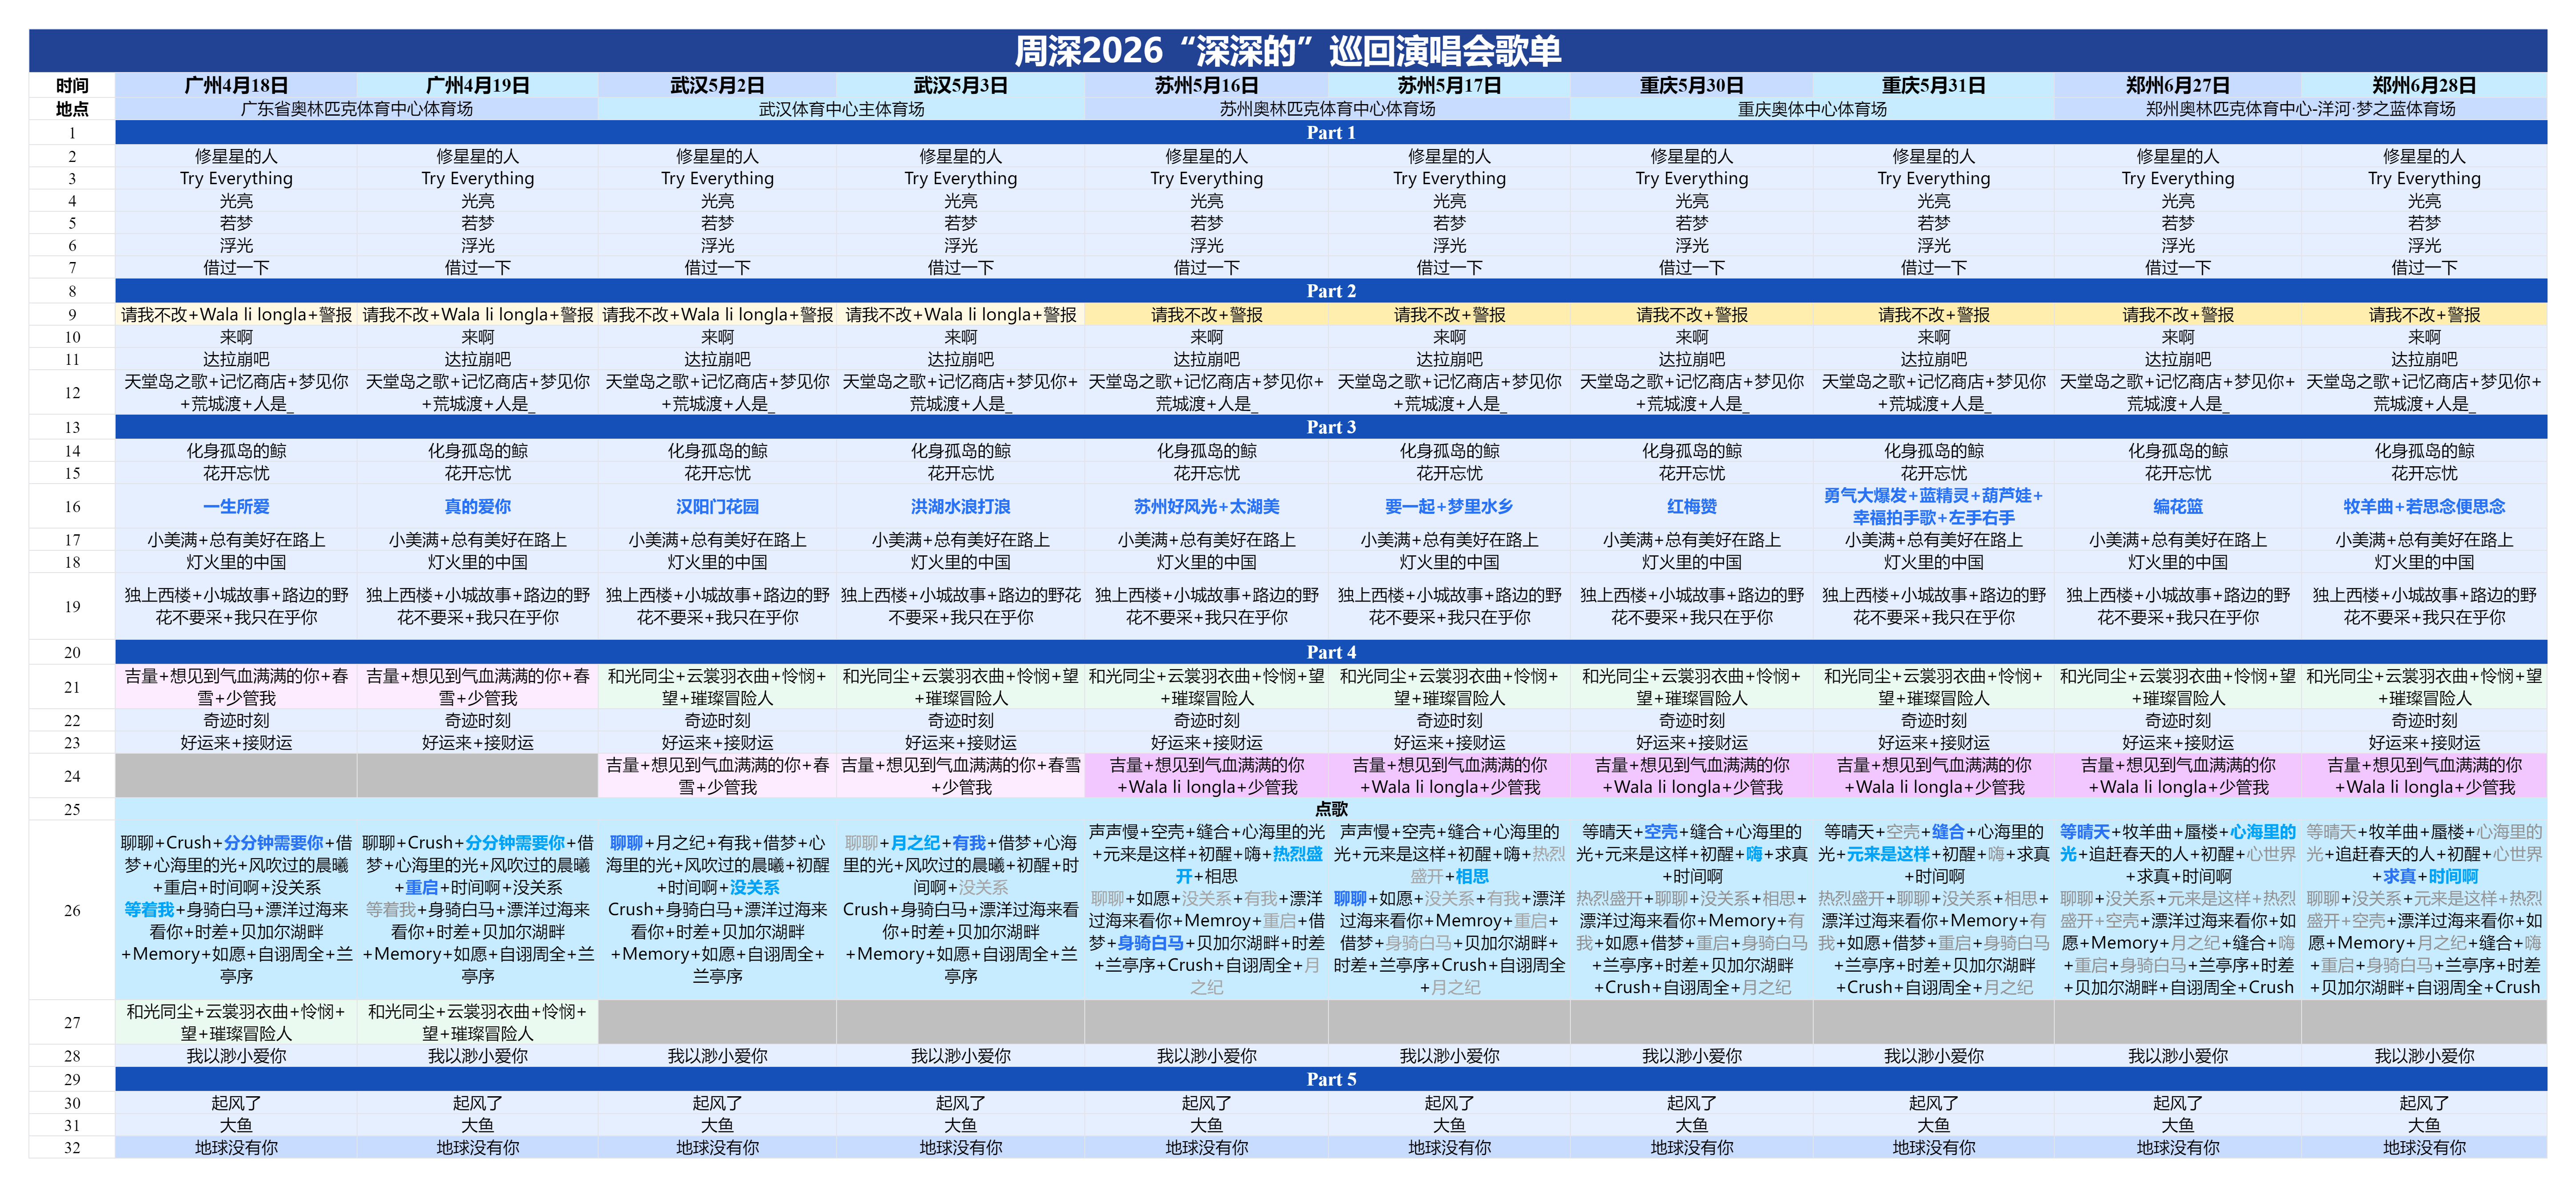
\includegraphics{img/playlists/playlists-shenshens2026-1} 

}

\caption{周深2026“深深的”巡回演唱会歌单}\label{fig:unnamed-chunk-64}
\end{figure}

\begin{figure}

{\centering 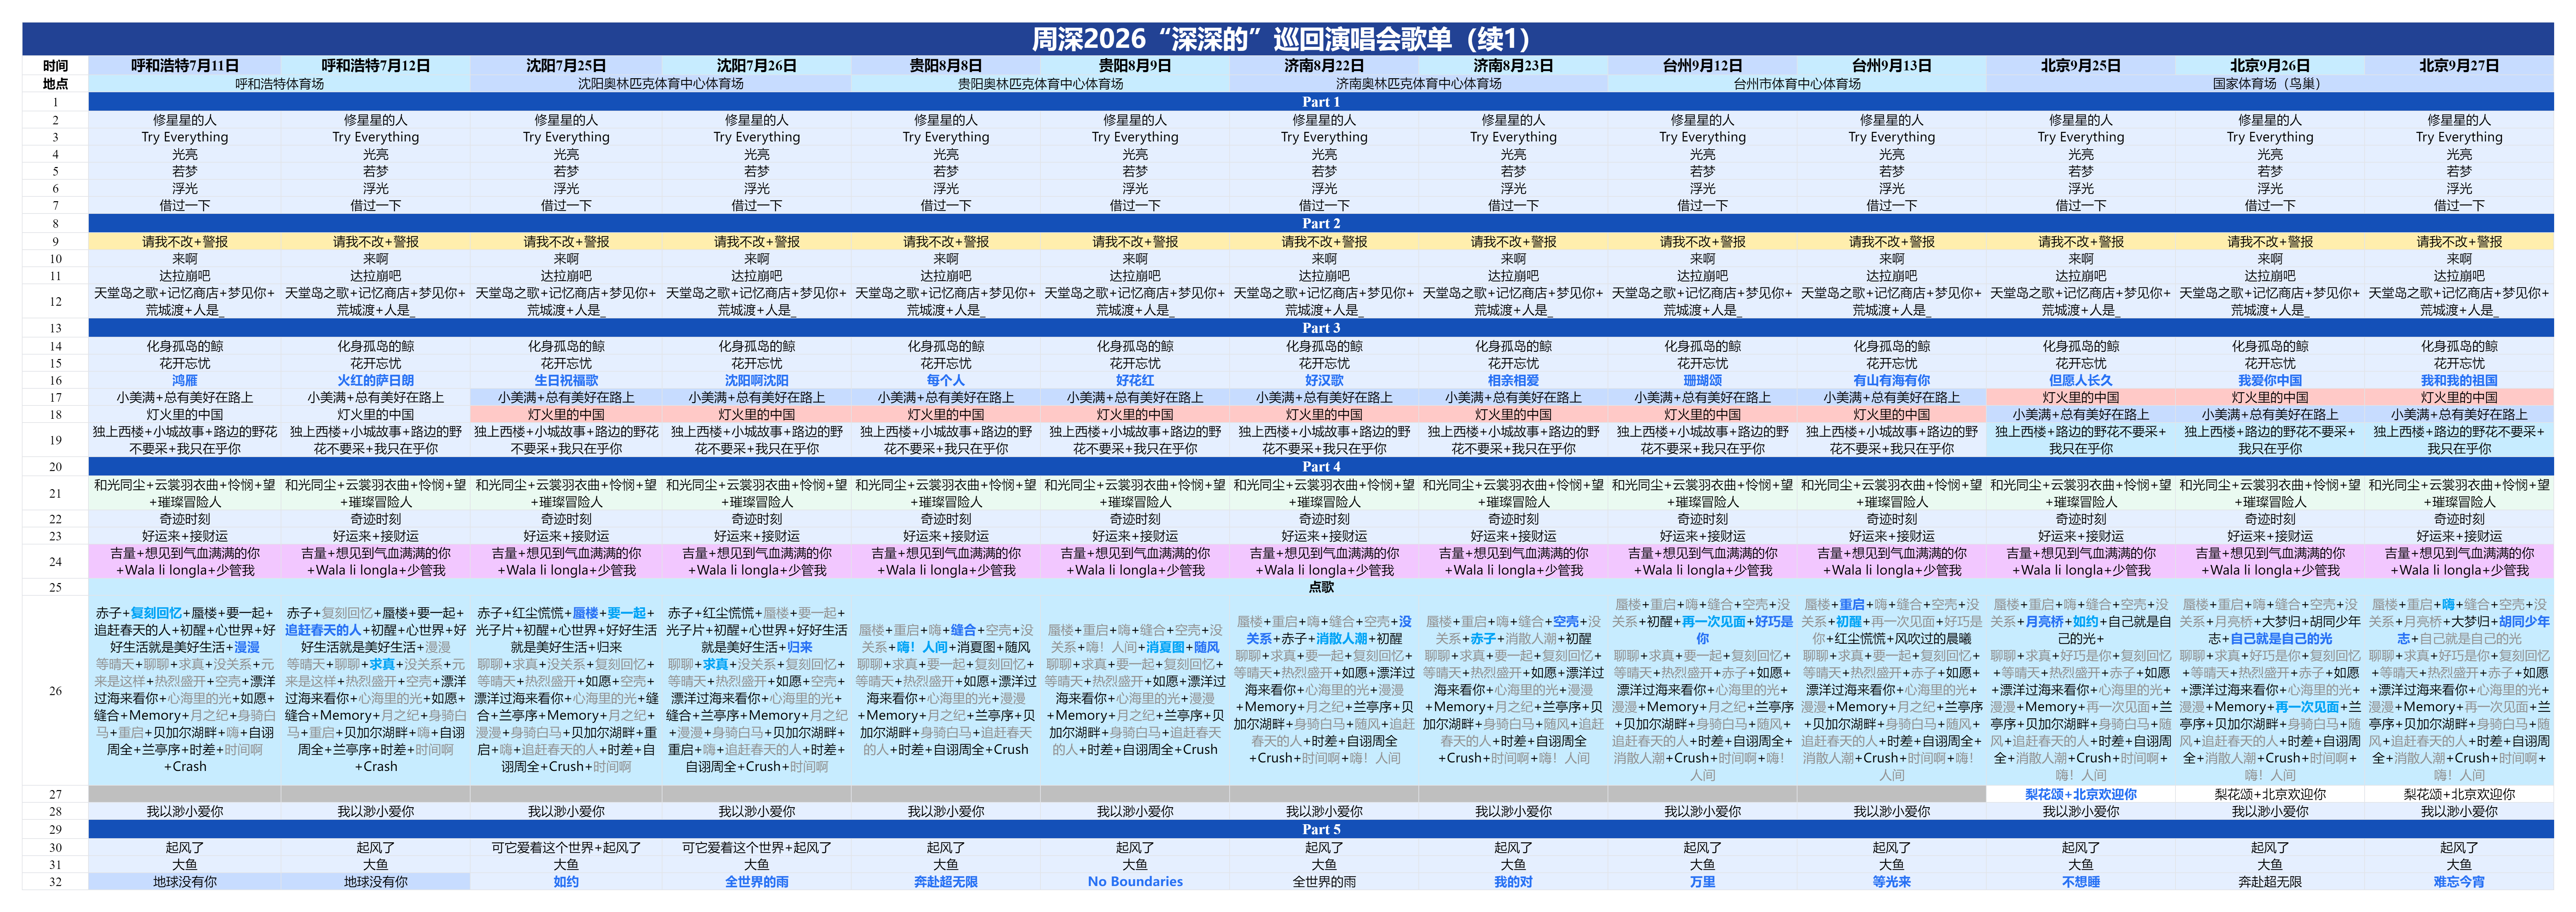
\includegraphics{img/playlists/playlists-shenshens2026-2} 

}

\caption{周深2026“深深的”巡回演唱会歌单（续1）}\label{fig:unnamed-chunk-65}
\end{figure}

\begin{figure}

{\centering 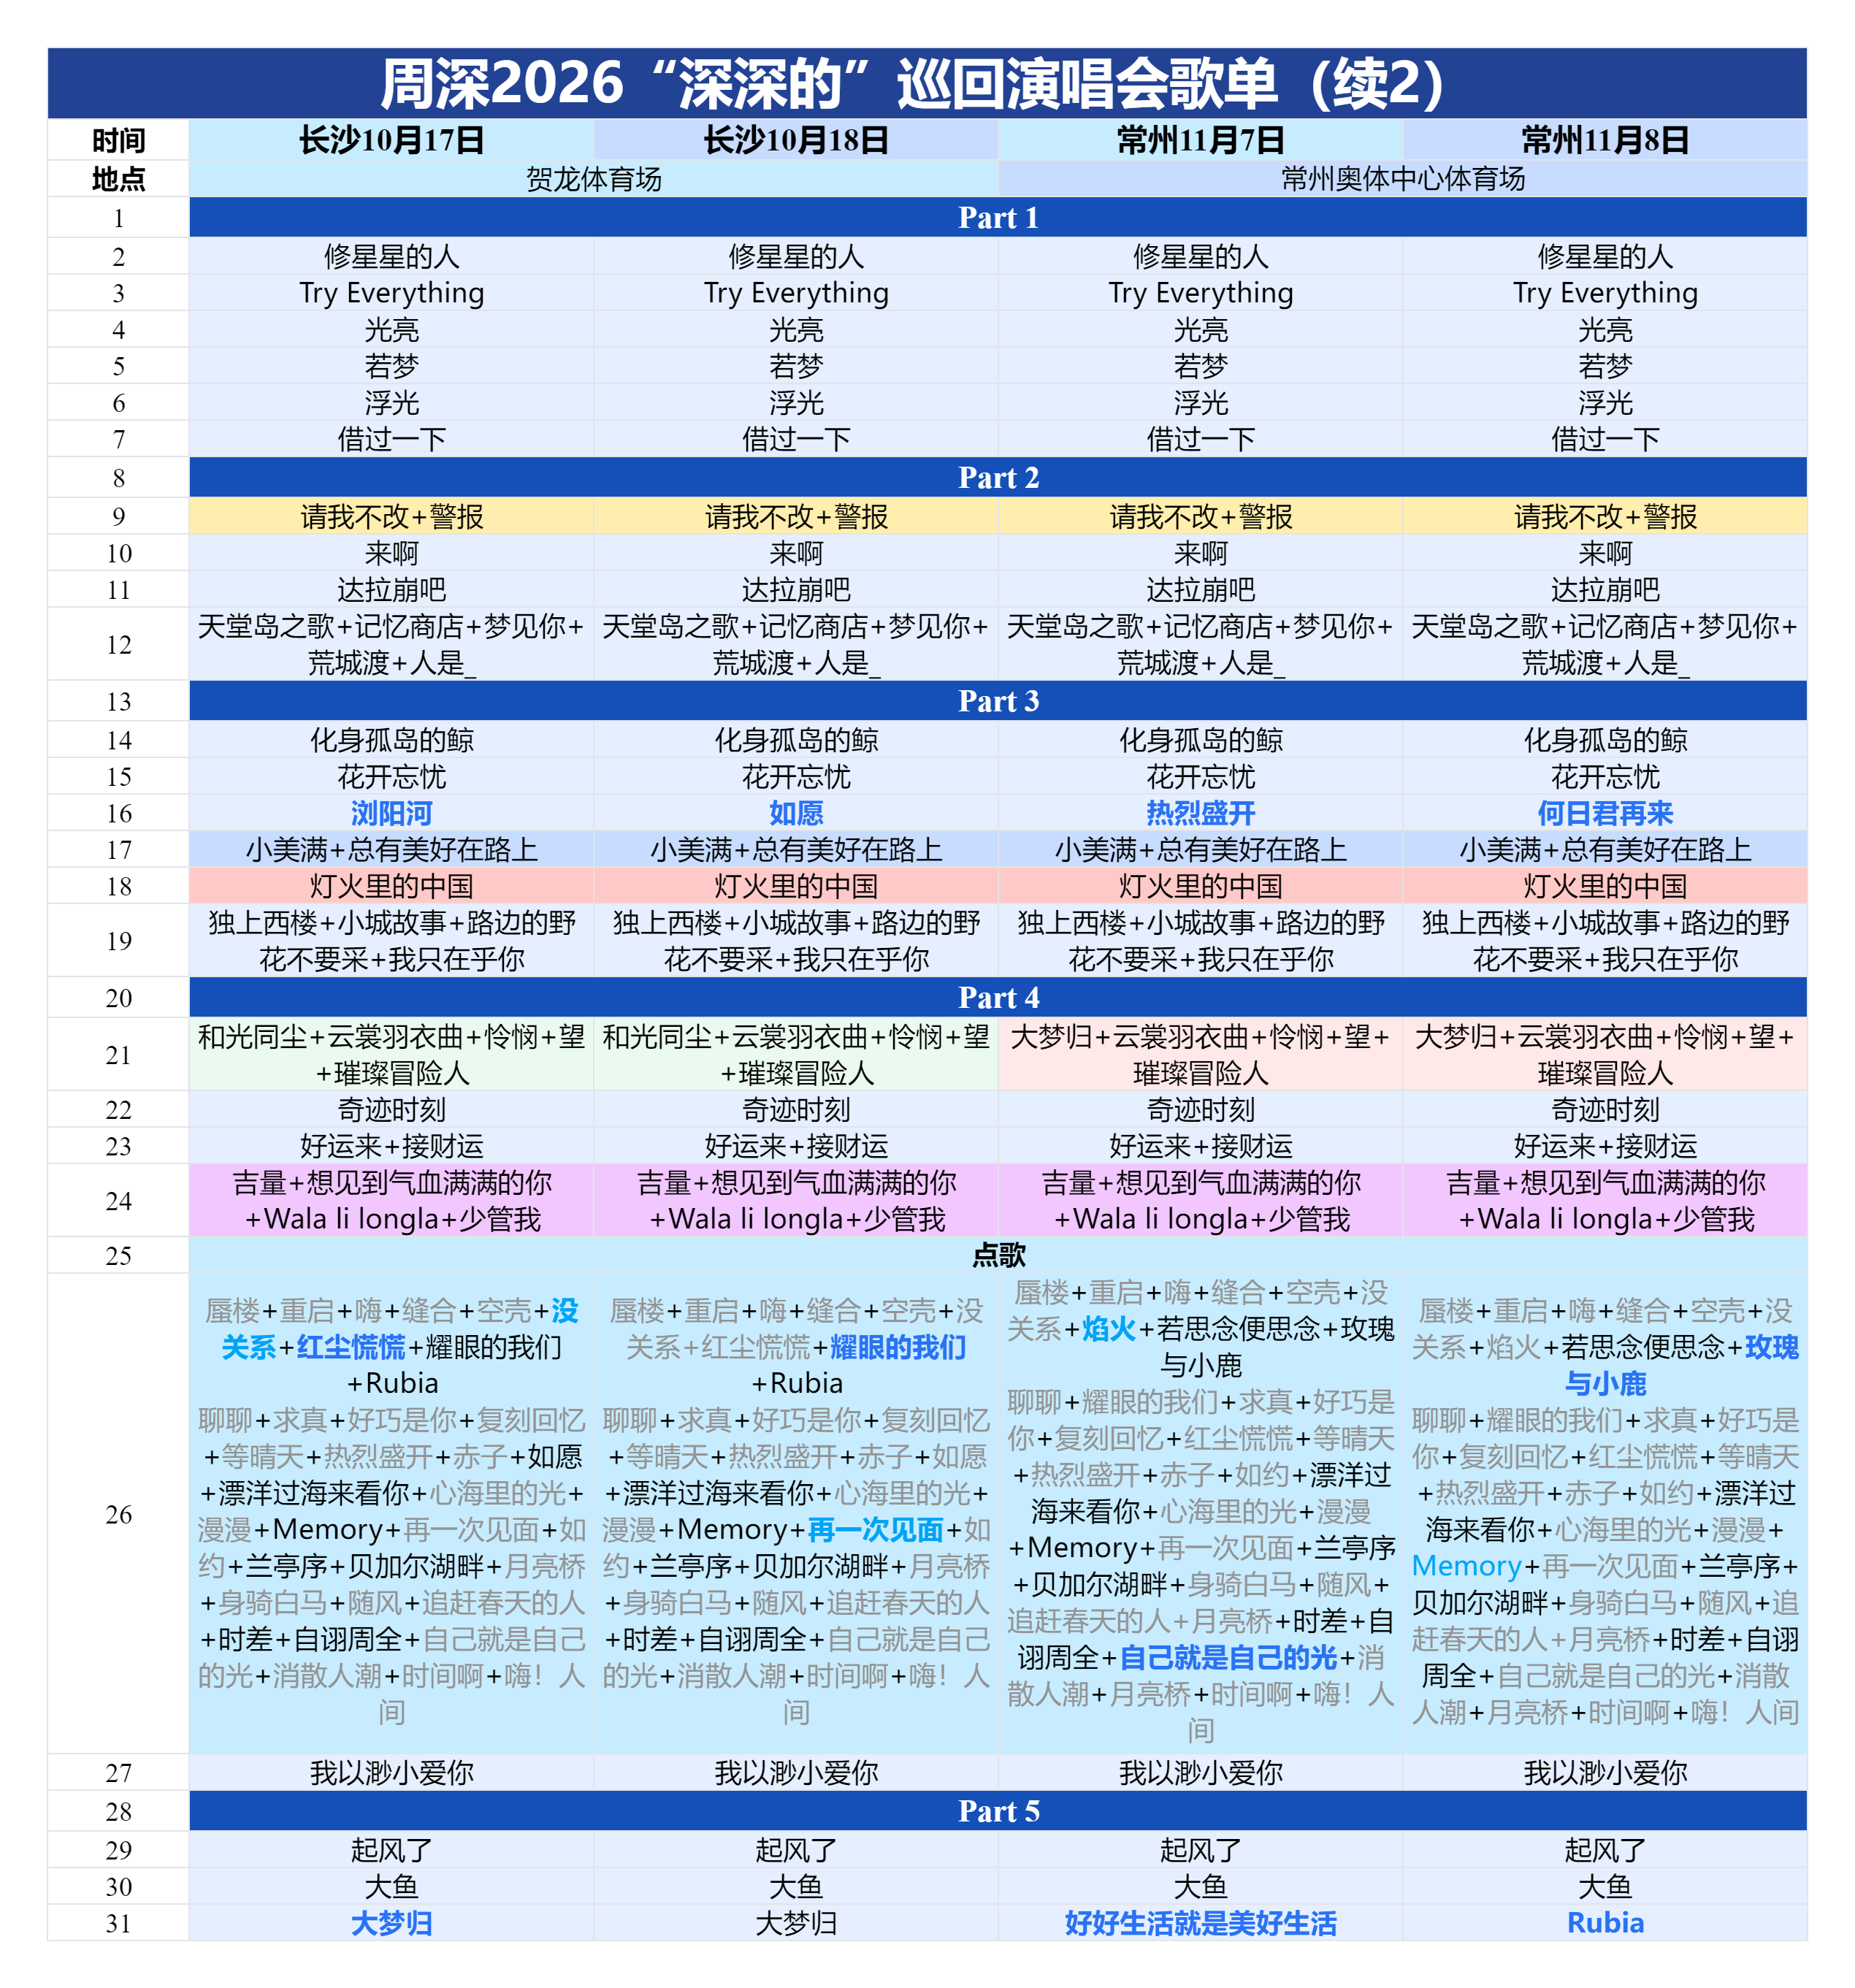
\includegraphics{img/playlists/playlists-shenshens2026-3} 

}

\caption{周深2026“深深的”巡回演唱会歌单（续2）}\label{fig:unnamed-chunk-66}
\end{figure}

\chapter{2026``深深的''巡回演唱会VCR文字版}\label{appendix-vcr-2026}

\section{开场VCR}\label{opening-vcr}

我们都是来自于一次宇宙大爆炸

1992年9月29日，我诞生了

你好，世界，你好

我是谁？

我是一颗尘埃

你是谁？

你是另一颗尘埃？

还是一片树叶，或者一只蝴蝶？

你也是第一次来到这颗星球吗？

你的眼睛是什么颜色呢？

我们会在哪个角落相遇呢？

在鲸鱼的背上

在桧树的脚印里〔听写待核，2025版为``在怪兽的脚印''〕

在平原、荒野

还是天空？

哇，夜空里有好多星星啊

它们是把外壳磨亮了吗？

它们是点燃了自己吗？

它们是自己造了翅膀飞那么高吗？

好想和它们一样啊

一眼就能被看见

那你呢？

你想成为什么呢？

我们去发着光的地方吧

去你的日记里

来我的日记里

你好

很高兴遇见你

我叫深深

深深的深深

\newpage

\section{机器人VCR}\label{robot-vcr}

二二二五年五月十七日

今天是我被选中执行任务的第两百天

系统维持正常运转的七万三千天

我是谁？

我每天都在重复着同样的工作

人类好有趣，有不一样的生活

人类好厉害

他们的伤口会自己愈合

会一起笑，会拥抱

会一起哭，会流泪

人类好有意思啊

我也想成为一个人

我也希望被爱着

爱，那是一个算法吗？

那是一串代码吗？

我是谁？

我能成为人吗？

一九九二零九二九号机器人

你自愿成为灵魂改造计划的首批志愿者

实验即将启动

并自行承担一切风险

是否确认？

我确认

机器人没有灵魂

但你们十分稳定

而且没有缺点，没有烦恼

而人类的灵魂会爱，会恨

会笑，会哭

会得到，会失去

会不舍，会放弃

会失败，也会成功

没关系

我想要拥有你说的这一切

我想成为人

我想知道，我是谁

好的，实验开始

\newpage

\section{音乐动画VCR}\label{music-animations-vcr}

〔本段为《化身孤岛的鲸》前的纯音乐动画，无旁白歌词。〕

\section{面具VCR}\label{mask-vcr}

2026年X月X日，XX

哇，这居然已经是我第三年开体育场巡回演唱会了

就算有那么多照片

我也不敢相信，居然真的做到了

哦不

应该说

你真的帮我做到了

我小时候都不敢做的那个最美的美梦

小的时候因为我的声音和大家不太一样

我就做了一个声音面具

把声音压低

然后发现真的就少了一些奇怪的眼光

我好像没有那么突兀了

好开心啊

终于可以融入大家喽

后来啊

我要在电视上唱歌

为了不让大家觉得我的声音奇怪

我就戴上了一个幺蛾子面具

还有一个背包客面具

这样他们就可以只听我唱歌

不看我的脸喽

那你呢？

你是不是也和我一样呢？

也有可以让自己变得和大家一样的面具？

本以为啊

我会一直戴着面具的

直到某一天我看到了你

你说，哎，你的声音好像有点不一样哦，我觉得

于是过了很久很久

我做了一个非常大胆的决定

我决定扯下面具来和你见面

好神奇啊

好像因为你的看见

我的不一样都被你的光照亮了

虽然你们都带着善意

称赞我怎么怎么好，怎么怎么厉害

虽然我还是会有很多不自信

但是谢谢你们看见了我

看见了面具背后那个不被喜欢的我

谢谢你们有耐心来听我唱歌

虽然我依然会怀疑自己是否值得被喜欢

虽然我依然没有办法做到

百分百自信和拥有十足的安全感

但是不用担心

人生日记本很厚很厚

还有那么多那么多空白页

只要写下去

只要和你们一起写下去

我相信我们一定能找到属于自己的答案的

你说，对吗？

\newpage

\section{交换日记VCR}\label{exchange-diaries-vcr}

〔背景音乐为《嗨！人间》〕

你好，我是周深

是你帮我找到了那个周深

有时候回头看

才发现那些不起眼的小事都可以是线索

就像是迷路时多绕的那些路

反而让我收获到了很多意想不到的风景

嗯，日记是什么呢？

我认为日记就像是没有任何目的去写的一个东西

写一些鸡毛蒜皮不重要的事情

也可以是天马行空突然想到的东西

在演完这么多场演出之后

我发现我这么多的随笔

这么多偶然的相遇

这么多迷茫的路

这么多你

帮我找到了我是谁

所以啊

请不要害怕你的人生日记会普通

会迷茫

会暂时找不到主题

只要写下去

就会精彩

你写你的迷茫，我也写着我的迷茫

写着写着，忽然就不迷茫了

因为翻到下一页的时候

你会发现

你还在

我也还在

接下来

让我们一起去寻找你

出发吧

\chapter{2026``深深的''巡回演唱会歌曲歌词}\label{appendix-song-lyric-2026}

\newpage

\section*{修星星的人}\label{xiu-xing-xing-de-ren}


\href{https://y.qq.com/n/ryqq_v2/songDetail/001LQ8ox0seA2B}{点击收听}

\begin{center}\rule{0.5\linewidth}{0.5pt}\end{center}

周深\\
词：董玉方\\
曲：胡帅\\
编曲：厉志腾/胡帅\\
制作人：胡帅\\
（电影《挽救计划》中文主题曲）

\begin{center}\rule{0.5\linewidth}{0.5pt}\end{center}

是我在故乡的旷野

仰望银河的夏夜

是我在宇宙的风暴

朝着天仓五飘曳

我的孤独 我的热烈

源自137亿年前

几粒星尘的蝴蝶

在噬星的幻灭里

给太阳撑一把雨伞

在时间的深海里

给地球道一声晚安

既然这宇宙让我诞生

想必它是要以我为证

我的情感和三十六度的体温

足以暖热即将熄灭的恒星

许我以造物的碎屑

重塑文明的边界

许我以渺小的羞怯

挽留物种的毁灭

我的勇敢 我的命运

来自几千几万光年外

漂浮的钠钾钙铁

在元素的聚散里

给人类抓一把糖果

在星海的倒影里

给生命升一簇篝火

既然这宇宙让我诞生

想必它是要以我为证

我的情感和三十六度的体温

足以暖热即将熄灭的恒星

既然这宇宙予我重生

想必它是要让我看懂

我的基因和闪闪发光的记忆

足以照亮所有星际的永恒

\section*{Try Everything}\label{try-everything}


\href{https://y.qq.com/n/ryqq_v2/songDetail/001tj9ip3ULdI4}{点击收听}

\begin{center}\rule{0.5\linewidth}{0.5pt}\end{center}

Shakira（周深翻唱）\\
词曲：Sia Furler/Mikkel Storleer Eriksen/Tor Erik Hermansen\\
（电影《疯狂动物城》主题曲）

\begin{center}\rule{0.5\linewidth}{0.5pt}\end{center}

Oh oh oh oh oh

Oh oh oh oh oh

Oh oh oh oh oh

Oh oh oh oh oh

I messed up tonight

I lost another fight

I still mess up but I'll just start again

I keep falling down

I keep on hitting the ground

I always get up now to see what's next

Birds don't just fly

They fall down and get up

Nobody learns without getting it wrong

I won't give up no I won't give in

Till I reach the end and then I'll start again

No I won't leave

I wanna try everything

I wanna try even though I could fail

I won't give up no I won't give in

Till I reach the end and then I'll start again

No I won't leave

I wanna try everything

I wanna try even though I could fail

Oh oh oh oh oh try everything

Oh oh oh oh oh try everything

Oh oh oh oh oh try everything

Oh oh oh oh oh

Look how far you've come

You filled your heart with love

Baby you've done enough take a deep breath

Don't beat yourself up

Don't need to run so fast

Sometimes we come last but we did our best

I won't give up no I won't give in

Till I reach the end and then I'll start again

No I won't leave

I wanna try everything

I wanna try even though I could fail

I won't give up no I won't give in

Till I reach the end and then I'll start again

No I won't leave

I wanna try everything

I wanna try even though I could fail

I'll keep on making those new mistakes

I'll keep on making them every day

Those new mistakes

Oh oh oh oh oh try everything

Oh oh oh oh oh try everything

Oh oh oh oh oh try everything

Oh oh oh oh oh

Try everything

\section*{光亮}\label{silver-linings}


\href{https://y.qq.com/n/ryqq/songDetail/001nWLsE4VJqC9}{点击收听}

\begin{center}\rule{0.5\linewidth}{0.5pt}\end{center}

周深\\
词：苏轼（北宋）/苟璘\\
曲：钱雷\\
编曲/制作人：钱雷

\begin{center}\rule{0.5\linewidth}{0.5pt}\end{center}

海上 一阵风吹起

白云涌向陆地

季风带走沙粒

四季 冷暖的交替

多鲜活的生命

又枯萎的痕迹

是奔跑中突然袭来的风雨

是黑暗中一根火柴燃烧的光明

也许你猜不透未知的宿命

像流星飞翔着它却不知目的

可是啊 我却 却愿意相信

最渺小最微弱最柔软最无畏的你

用尽了全力 努力地回应

再无边再无尽再无解总有一线生机

光亮你自己

戏曲念白：

莫听穿林打叶声

一蓑烟雨任平生

畅音阁里终一叙

六百年一粟 沧海一梦

可是啊 我却 却愿意去相信

最渺小最微弱最柔软最无畏的你

用尽了全力 努力地去回应

再无边再无尽再无解总有一线生机

光亮你自己

戏曲唱腔：

莫听穿林打叶声

一蓑烟雨任平生

畅音阁里终一叙

六百年一粟 沧海一梦

无论目的 最无畏的你

不问宿命 最无畏的你

\section*{若梦}\label{like-a-dream}


\href{https://y.qq.com/n/ryqq/songDetail/002Id4Xd0F98go}{点击收听}

\begin{center}\rule{0.5\linewidth}{0.5pt}\end{center}

周深\\
词：王明毓\\
曲：和汇慧/王梓同\\
编曲：王子操 (马来西亚)

\begin{center}\rule{0.5\linewidth}{0.5pt}\end{center}

浮生若梦 为欢几何

风摇雨落 此心何处停泊

剑起刀割 却斩不断这因果

看天地之间皆漠漠

尘缘萧索 宿命奈何

日升月落 此生依旧难舍

铁马金戈 也踏不碎这心火

忆前尘旧梦 任岁月 消磨

往事流转在你眼眸

一边遗忘 一边拼凑

如我虔诚合十双手

唯愿你能得到拯救

情缘若梦 长久几何

一枕寒宵 饮下苦涩独酌

杯酒当歌 却绕不开这心锁

愿清欢入梦 伴此心 停泊

往事流转在你眼眸

一边遗忘 一边拼凑

如我虔诚合十双手

唯愿你能得到拯救

往事流转在你眼眸

一边遗忘 一边拼凑

如我虔诚合十双手

唯愿你能得到拯救

唯愿你能得到拯救

\section*{浮光}\label{floating-light}


\href{https://music.163.com/\#/song?id=2112196350}{点击收听}

\begin{center}\rule{0.5\linewidth}{0.5pt}\end{center}

周深\\
作词 : 唐思淼/邹念慈\\
作曲 : Jannik\\
编曲：曾吴秋杰\\
原编曲：Jannik

\begin{center}\rule{0.5\linewidth}{0.5pt}\end{center}

看指尖拨响蝴蝶 扇动一场离别

我推开无声岁月 续梦一页

你我只是打个照面 可曾有过誓约

走进熟悉却 陌生的思念

啊\ldots\ldots{}

啊\ldots\ldots{}

你的眼眸装满了时间

你的身后拥故事成篇

此生如梦愿细数流年

与你同写 沧海桑田

浮光掠影重山彩云间

你的伏线穿越千百年

人生不过恍惚三万天

漫漫人间 留恋流连

你说那月光 照过同样城墙

永恒的刹那的 此刻沉默无话

想问你这星空 是否不曾变

是啊 是啊

我们望着它

风吹过耳旁 古远的歌唱啊

这是我也是你 不曾遗忘的啊

是来路是去处 是你在回答

去吧 去啊

总会相遇吧

你的眼眸装满了时间

你的身后拥故事成篇

此生如梦愿细数流年

与你同写 沧海桑田

浮光掠影重山彩云间

你的伏线穿越千百年

人生不过恍惚三万天

漫漫人间 留恋流连

\section*{借过一下}\label{excuse-me}


\href{https://y.qq.com/n/ryqq/songDetail/00446BOH0yUBXf}{点击收听}

\begin{center}\rule{0.5\linewidth}{0.5pt}\end{center}

周深\\
词：唐恬\\
曲：周以力\\
制作人/编曲：周以力

\begin{center}\rule{0.5\linewidth}{0.5pt}\end{center}

少年扬起脸庞 前往他的月亮

人们笑他狂妄 人怎可不一样

白衣过泥潭 怎敢说不染

但凡银两有价 谁能真潇洒

少年爬上城墙 去见他的月亮

破碎几次心脏 得来几句真相

市井或朝堂 四方皆如框

若你生来有刺 磨掉再入场

你们都是对的他说拜托

让开一下

让我大醉一场 殿堂之上

背闲诗两三章

让我穿白衣裳 过疯人巷

去泥潭捞月光

望大人们见谅 提点的话

我懂也不想装

世人寻黄金乡 我找月亮

何必同往

话谢过 路借过 你是你 我是我

话谢过 路借过 你是你 我是我

诚如先生所说 每颗心都有瑕

潇洒不是不怕 是愿付出代价

权衡利弊后 仍守对与错

谢过赐教的话 路借过一下

让我大醉一场 殿堂之上

背闲诗两三章

让我穿白衣裳 过疯人巷

去泥潭捞月光

望大人们见谅 提点的话

我懂也不想装

世人寻黄金乡 我找月亮

何必同往

话谢过 路借过 你是你 我是我

话谢过 路借过 你是你 我是我

白衣过泥潭 世故里浪漫

知心有所爱 不更改

人见过明暗 若天真犹在

当披上月光 走夜晚

\newpage

\section*{请我不改}\label{brave-heart}


\href{https://y.qq.com/n/ryqq/songDetail/002qdxkv42Tpzb}{点击收听}

\begin{center}\rule{0.5\linewidth}{0.5pt}\end{center}

周深\\
词：尹约\\
曲：钱雷\\
编曲：钱雷\\
制作人：钱雷

\begin{center}\rule{0.5\linewidth}{0.5pt}\end{center}

是谁在我 耳边念白

说我不配 我不够好 我必失败

是谁将我 双眼遮盖

惩罚我坠入百无一用的黑暗

是谁不断 日夜合围 向我追来

痛击我最脆弱短板

是谁模糊 我的未来

恐惧淹没了期待

绝望已经大军压境

回身却没半个人影

才看清追兵与逃兵

竟都是我自己

请我不改 我的姿态

我的爱我的痛都与生俱来

请我看开 我的存在

我的明我的暗都不必躲开

我原谅我自己 捡起遗憾拥抱无奈

我允许我放手 让我勇敢活在现在

我不等待 我不徘徊

我的笑我的泪都不再苍白 放肆盛开

(Brave heart)

(Brave heart)

(Brave heart)

是谁不断 日夜合围 向我追来

痛击我最脆弱短板

是谁模糊 我的未来

恐惧淹没了期待

绝望已经大军压境

回身却没半个人影

才看清追兵与逃兵

竟都是我自己

请我不改 我的姿态

我的爱我的痛都与生俱来

请我看开 我的存在

我的明我的暗都不必躲开

我原谅我自己 捡起遗憾拥抱无奈

我允许我放手 让我勇敢活在现在

我不等待 我不徘徊

我的笑我的泪都不再苍白 放肆盛开

(Brave heart)

(Brave heart)

(Brave heart)

暗无天日辗转痛楚

蚌壳终于吐出明珠

微弱光点汇成光束

我向日出更近一步

请我不改 我的姿态

我的爱我的痛都与生俱来

请我看开 我的存在

我的明我的暗都不必躲开

我原谅我自己 捡起遗憾拥抱无奈

我允许我放手 让我勇敢活在现在

我不等待 我不徘徊

我的笑我的泪都不再苍白 坦荡痛快

\section*{警报}\label{jing-bao}


\href{https://y.qq.com/n/ryqq_v2/songDetail/001Ms67n2CZw1q}{点击收听}

\begin{center}\rule{0.5\linewidth}{0.5pt}\end{center}

周深\\
词：尹约\\
曲：钱雷\\
（专辑《反深代词》）

\begin{center}\rule{0.5\linewidth}{0.5pt}\end{center}

迁就对方的节奏

感受对方的感受

请求对方的请求

成就对方的成就

原地不动 不忍失守

你等在情绪代谢的最下游

予取予求 照单全收

别人的任性汹涌

为何你心情表情从来不相通

为何你伤得越重笑得越轻松

不停点头 不折不扣

一付出就是全部的最上游

毫无保留 倾你所有

竟还担心不够

我发送 警报声 血红色 惊叹号

提醒你自救

被遥控 被耗空 快失控 快断送

我替你看透

从借用 到利用 到享用 到滥用

转身就走

他们绝不 为你而痛

共情是一种劳动

温柔是一种苦衷

善良是一种沉重

原谅是一种纵容

人前人后 思前想后

你被困进人情世故的中游

为难左右 无力追究

你终将何去何从

为何你心情表情从来不相通

为何你内心越痛笑得越隆重

千疮百孔 暗藏担忧

你却看不见自己快要断流

回应落空 希望尘封

求救无人听懂

我不断 再计算 因为你 不计算

还能撑多久

给世界 最宽容 给自己 最苛求

顺位排最后

你心口 从伤口 到决口 不开口

笑容始终

我学会痛 为你而痛

\section*{来啊}\label{lai-a}


\href{https://y.qq.com/n/ryqq/songDetail/003V4lkA1dpSrC}{点击收听}

\begin{center}\rule{0.5\linewidth}{0.5pt}\end{center}

周深\\
词：小麻M.Refre\(H
曲：小麻M.Refre\)H\\
制作人：郑楠(SBMS)

\begin{center}\rule{0.5\linewidth}{0.5pt}\end{center}

我 我怎么就这样呆头呆脑

一不小心 落入圈套

沉迷的神魂颠倒

Pass off

这灵魂乱七八糟

我 瞳孔里都是你迷人的笑

越靠越近 我越浮躁

神涣散虚无缥缈

Cut stop

躁动太纷纷扰扰

天生的怪胎

（你啊）

踌躇着徘徊

（你啊）

太嘈杂的时代

1v1较量打乱了节拍

（咿呀）

别气急败坏

（你啊）

别着急淘汰

（你啊）

一万种防备阻碍

不如就算了

靠过来

将错就错

别拖Let's go

随你 操控

But

Don't tell me lie eeeee

Lie eeee

我望眼欲穿你别闪躲

Don't tell me lie eeee

Lie eeee

要爱就爱放纵吧 别退缩

Don't tell me lie eeeee

Lie eeee

我倾其所有赴汤蹈火

Don't tell me lie eeeee

Lie eeee

敢不敢直视我

Let's fall

我 瞳孔里都是你迷人的笑

越靠越近 我越浮躁

神涣散虚无缥缈

Cut stop

躁动太纷纷扰扰

天生的怪胎

（你啊）

踌躇着徘徊

（你啊）

太嘈杂的时代

1v1较量打乱了节拍

（咿呀）

别气急败坏

（你啊）

别着急淘汰

（你啊）

一万种防备阻碍

不如就算了

靠过来

将错就错

别拖Let's go

随你 操控

But

Don't tell me lie eeeee

Lie eeee

我望眼欲穿你别闪躲

Don't tell me lie eeee

Lie eeee

要爱就爱放纵吧 别退缩

Don't tell me lie eeeee

Lie eeee

我倾其所有赴汤蹈火

Don't tell me lie eeeee

Lie eeee

敢不敢直视我

Let's fall

\section*{达拉崩吧}\label{dalabengba}


\href{https://y.qq.com/n/ryqq/songDetail/002kN8FY1hPhAC}{点击收听}

\begin{center}\rule{0.5\linewidth}{0.5pt}\end{center}

周深\\
词：ilem\\
曲：ilem\\
编曲：孔潇一\\
原唱：洛天依/言和\\
Program：孔潇一\\
制作人：孔潇一

\begin{center}\rule{0.5\linewidth}{0.5pt}\end{center}

小女孩：

很久很久以前 巨龙突然出现

带来灾难 带走了公主又消失不见

王国十分危险 世间谁最勇敢

一位勇者赶来 大声喊

少年：

我要带上最好的剑 翻过最高的山

闯进最深的森林 把公主带回到面前

小女孩：

国王非常高兴 忙问他的姓名

年轻人想了想 他说

陛下我叫

达拉崩吧斑得贝迪卜多比鲁翁

国王：

再说一次

少年：

达拉崩巴斑得贝迪卜多比鲁翁

国王：

是不是

达拉崩吧斑得贝迪卜多比鲁翁

少年：

对对 达拉崩巴斑得贝迪卜多比鲁翁

旁白：

英雄达拉崩吧 骑上最快的马

带着大家的希望从城堡里出发

战胜怪兽来袭 获得十二金币

无数伤痕见证 他慢慢升级

小女孩：

偏远美丽村庄 打开所有宝箱

一路风霜伴随指引前路的圣月光

闯入一座山洞 公主和可怕的巨龙

英雄拔出宝剑 巨龙说

巨龙：

我是 昆图库塔卡提考特苏瓦西拉松

少年：

再来一次

巨龙：

昆图库塔卡提考特苏瓦西拉松

少年：

是不是 昆特牌提琴

烤蛋挞 苏打 马拉松

巨龙：

不对

是昆图库塔卡提考特苏瓦西拉松

旁白：

于是

少年：

达拉崩巴斑得贝迪卜多比鲁翁

旁白：

砍向

巨龙：

昆图库塔卡提考特苏瓦西拉松

旁白：

然后

巨龙：

昆图库塔卡提考特苏瓦西拉松

旁白：

咬了

少年：

达拉崩吧斑得贝迪卜多比鲁翁

旁白：

最后

达拉崩巴斑得贝迪卜多比鲁翁

他战胜了

巨龙：

昆图库塔卡提考特苏瓦西拉松

旁白：

救出了

公主米娅莫拉苏娜丹妮谢莉红

回到了

蒙达鲁克硫斯伯古比奇巴勒城

国王听说

达拉崩巴斑得贝迪卜多比鲁翁

他打败了

昆图库塔卡提考特苏瓦西拉松

就把 公主米娅莫拉苏娜丹妮谢莉红

嫁给

达拉崩吧斑得贝迪卜多比鲁翁

啦啦 达拉崩巴 公主米娅

幸福得像个童话

他们生下一个孩子

也在天天渐渐长大

为了避免以后麻烦 孩子称作王浩然

他的全名十分难念 要念你来念吧

\section*{天堂岛之歌}\label{haven-song}


\href{https://y.qq.com/n/ryqq/songDetail/000gUmh94eXmmP}{点击收听}

\begin{center}\rule{0.5\linewidth}{0.5pt}\end{center}

周深

\begin{center}\rule{0.5\linewidth}{0.5pt}\end{center}

叮咚

我有一个秘密

悄悄告诉你

欢迎你来到天堂入口

叮咚

有人在按门铃

是谁在外面

把恶作剧当一种游戏

听啊 谁在哭泣

看啊 谁在窃窃私语

窗外有双眼睛

它在时刻注视着你

叮咚

我在这里等你

你在等我吗

是什么原因让你害怕

叮咚

你会藏在哪里

别想要逃离

想逃出手心已来不及

被遗忘的记忆

被你藏起来的秘密

不要大声呼吸

你已暴露了你自己

啊啊啊

Knock knock 外面下起了雨

放弃挣扎吧

谎言说多了就会发现

Knock knock 是谁在做坏事

假装成幸运

我总会找到你在床底

听呐 你在恐惧

看呐 你在歇斯底里

窗外有双眼睛

他在时刻注视着你

叮咚

有人在看你的过去

叮咚

有人在看你的秘密

叮咚

有人在看你的过去

叮咚

我逃不出去

啊啊啊

\section*{记忆商店}\label{the-memory-store}


\href{https://y.qq.com/n/ryqq/songDetail/0047wVWr3JcjfC}{点击收听}

\begin{center}\rule{0.5\linewidth}{0.5pt}\end{center}

周深\\
词：唐恬\\
曲：Paula Winger/Cash Callaway/Sarah Haglund\\
编曲：Paula Winger/Cash Callaway/Sarah Haglund\\
制作人：钱雷

\begin{center}\rule{0.5\linewidth}{0.5pt}\end{center}

有客人从 夜里来

买很古老 的年代

记忆的 货品单

这一款 早售完

不虚拟的拥吻 想不想买

没噩梦的睡眠 耳边goodnight

找遍了 记忆商店

他说想 再荡个秋千

妈妈我想飞得高点

星球以 光速穿越

妈妈我 想落到地面

荡啊荡啊荡个秋千

摇啊晃啊去找花园

买鲸鱼歌声呜咽

岛屿还未消失 这个世界还曾 下着雪

亲爱的 我很抱歉

不朽的 没有了 没人记得

有新款流星雨 人群狂欢

有温暖的炉火 不需要下载 的陪伴

找遍了 记忆商店

他说想 再荡个秋千

妈妈我想飞得高点

星球以 光速穿越

妈妈我 想落到地面

荡啊荡啊荡个秋千

摇啊晃啊去找花园

要找我的秋千

只需要 荡起脚尖

只需要 等着落地

没什么 要明白 没什么 要勇敢

荡啊荡啊荡个秋千

\section*{梦见你}\label{meng-jian-ni}


\href{https://y.qq.com/n/ryqq_v2/songDetail/004bnFMj49UFJY}{点击收听}

\begin{center}\rule{0.5\linewidth}{0.5pt}\end{center}

周深\\
词：沃特艾文儿\\
曲：钱雷\\
（电影《时间之子》主题曲/片尾曲）

\begin{center}\rule{0.5\linewidth}{0.5pt}\end{center}

我终于在 某一个梦里

重新见到 还年少的你

时隔多年 又坐在一起

依旧像未曾分离那样亲密

关于你的 都说来听听

许多事情 我已记不清

他日远行 若遇你爱的风景

我定会长久地驻足替你 看得更用心

当再一次听你喊出我姓名

我已将一生都历经

明白有些事情早注定

我们都站在 时间的河里

离别是相遇的倒影

从初问候的 那天起

就 有了再见的回音

如此也要走向你

看着眼前 还年少的你

恍如流年 从未淌过去

时光飞逝 就算我已经老去

你却仍有着初见时那双 清澈的眼睛

当再一次听你喊出我姓名

我已将一生都历经

明白有些事情早注定

我们都站在 时间的河里

离别是相遇的倒影

从初问候的 那天起

就 有了再见的回音

我望着你 远去的背影

渐行渐远 直到看不清

时间会改变一切

却再也无法改变你

若多年后 还能够有幸

与你重逢 在另场梦境

但愿那时你在人海里

仍将我一眼认清

可当我再一次喊出你姓名

通天彻地都 没回应

整个世界刹那间安静

每当想起你 一切都暂停

时间的河像结了冰

我亲爱的你 不必醒

就 睡在我的回忆里

你将永远都年轻

\section*{荒城渡}\label{huang-cheng-du}


\href{https://y.qq.com/n/ryqq_v2/songDetail/002JueG342RaZZ}{点击收听}

\begin{center}\rule{0.5\linewidth}{0.5pt}\end{center}

周深\\
词：张赢\\
曲：夏恒/邓强中\\
编曲：于韵非\\
（《陈情令》薛洋人物曲）

\begin{center}\rule{0.5\linewidth}{0.5pt}\end{center}

眼中拂尘 手中残魂

那故事斑驳荒城

修炼天真 拨开心门

握一颗糖暖这孤身颠簸

命运多残忍 最怕饮恨

耗尽余生是否能重生

一等再等 善恶终分 羽化星辰

夜色中寻觅过

当往事困住我

也盼心中生出一点萤火

孤城的传说 有谁来过

将因果赠与我

我在等这因果

渡魂渡魄渡我

纵然已是 执着难舍

断了这心魔 可原谅我

宿命中获得 这解脱 重来过

已知命运多残忍

不看不问不怨不恨

等待中重生为一个人

人世浮沉 无悔此生

夜色中寻觅过

当往事困住我

也盼心中生出一点萤火

孤城的传说 有谁来过

将因果赠与我

我在等这因果

渡魂渡魄渡我

纵然已是 执着难舍

断了这心魔 可原谅我

宿命中获得 这解脱 重来过

\section*{人是\_}\label{Humans_are_}


\href{https://y.qq.com/n/ryqq/songDetail/001zuNRq15kB7v}{点击收听}

\begin{center}\rule{0.5\linewidth}{0.5pt}\end{center}

周深\\
词：唐恬\\
曲：钱雷\\
编曲：钱雷\\
制作人：钱雷

\begin{center}\rule{0.5\linewidth}{0.5pt}\end{center}

去往 所有 命运 风暴之中的盲童

你来自火山炙热 与苦寒的深海

生本 就是 意外 硬币反选为尘埃

为侥幸可以相爱 造了船 移着山

出征是古老的宿命

人将赤足踏入夜晚

只有我可以来决定 我以何种姿态

让死亡觊觎我

让恐惧亲吻我

来摧毁我深爱的一切

可仍夺不走我的选择

弹指间湮灭我

但命运打不败活着

让生命如剧烈的烟火

璀璨熄灭前也将点亮

孩童的双眸

未知 摊开 棋局 舍弃昨日才可破

再见了我的月光 我的蓝 我的爱

钢铁的巨兽在轰鸣 我们拒绝走入夜晚

破碎是新生的约定 我便愿为尘埃

让死亡觊觎我

让恐惧亲吻我

来摧毁我深爱的一切

可仍夺不走我的选择

弹指间湮灭我

但命运打不败活着

让生命如剧烈的烟火

璀璨熄灭前也将点亮

孩童的双眸

若巨浪已淹没了来路 我是帆 亦是舟

是微渺 的希望

我们依然前行 没有光指引

往前吧 失去吧 不要停留

让时空消亡我

你无需记得我

来摧毁我深爱的一切

可仍夺不走我的选择

弹指间湮灭我

但命运打不败活着

是微茫中高歌的族类

生命像烟火那就点亮

孩童的双眸

未来的瞳孔

\newpage

\section*{化身孤岛的鲸}\label{The-whale-who-became-an-island}


\href{https://y.qq.com/n/ryqq/songDetail/0004adDk3wsULz}{点击收听}

\begin{center}\rule{0.5\linewidth}{0.5pt}\end{center}

周深\\
词：沃特艾文儿\\
曲：徐浩\\
编曲/制作人：唐汉霄

\begin{center}\rule{0.5\linewidth}{0.5pt}\end{center}

我是只化身孤岛的蓝鲸

有着最巨大的身影

鱼虾在身侧穿行

也有飞鸟在背上停

我路过太多太美的奇景

如同伊甸般的仙境

而大海太平太静

多少故事无人倾听

我爱地中海的天晴

爱西伯利亚的雪景

爱万丈高空的鹰

爱肚皮下的藻荇

我在尽心尽力地多情

直到那一天

你的衣衫破旧

而歌声却温柔

陪我漫无目的的四处漂流

我的背脊如荒丘

而你却微笑摆首

把它当成整个宇宙

你与太阳挥手

也同海鸥问候

陪我爱天爱地的四处风流

只是遗憾你终究

无法躺在我胸口

欣赏夜空最辽阔的不朽

把星子放入眸

我是只化身孤岛的蓝鲸

有着最巨大的身影

鱼虾在身侧穿行

也有飞鸟在背上停

我有着太冷太清的天性

对天上的她动过情

而云朵太远太轻

辗转之后各安天命

我未入过繁华之境

未听过喧嚣的声音

未见过太多生灵

未有过滚烫心情

所以也未觉大洋正中

有多么安静

你的衣衫破旧

而歌声却温柔

陪我漫无目的的四处漂流

我的背脊如荒丘

而你却微笑摆首

把它当成整个宇宙

你与太阳挥手

也同海鸥问候

陪我爱天爱地的四处风流

只是遗憾你终究

无法躺在我胸口

欣赏夜空最辽阔的不朽

把星子放入眸

你的指尖轻柔

抚摸过我所有

风浪冲撞出的丑陋疮口

你眼中有春与秋

胜过我见过爱过

的一切山川与河流

曾以为我肩头

是那么的宽厚

足够撑起海底那座琼楼

而在你到来之后

它显得如此清瘦

我想给你能奔跑的岸头

让你如同王后

\section*{花开忘忧}\label{Blossoms-that-forget-sorrow}


\href{https://y.qq.com/n/ryqq/songDetail/004czGF42WSgko}{点击收听}

\begin{center}\rule{0.5\linewidth}{0.5pt}\end{center}

周深\\
词：唐恬\\
曲：钱雷\\
编曲：钱雷\\
制作人：钱雷

\begin{center}\rule{0.5\linewidth}{0.5pt}\end{center}

巷子口 买了花

穿过沿街红墙青瓦

夕阳慢慢亲吻着 我的白发

推开旧木门 回到家

把时光 都炖香

而你只是笑 不说话

一件遗憾的事 就喝一碗汤

庭院深深 秋叶飘落

我们苍老的时候 就回到小时候

采青梅用来酿酒你 不许偷着喝

穿朴素的衣裳 牵着那衣袖

捡了小猫 名为苍狗

我们睡去的时候 像孩子无忧愁

反正也很难上锁这 岁月如小偷

若记忆被偷走了 忘了我的爱

我会说 你好啊

这是给 你的花

花的名字叫忘忧草

它说时光汹涌 如水上烟波

别走远了 一起回家

我们苍老的时候 就回到小时候

采青梅用来酿酒你 不许偷着喝

穿朴素的衣裳 牵着那衣袖

捡了小猫 名为苍狗

我们睡去的时候 像孩子无忧愁

在梦里做个梦 看见你我都老了

那永恒没骗我 离散也没有

这份爱只是活在 另外时空

如果 每一声再见 会开启

一个新的空间

每做一个梦 是时空 偶尔的重叠

你好吗 离开的人啊

请帮我 相爱到剧终

忘忧草 开着花

你在月光下 不说话

一件遗憾的事 就喝一杯茶

庭院深深 秋叶飘落

\section*{小美满}\label{simple-bliss}


\href{https://y.qq.com/n/ryqq/songDetail/002QvWwX1BG9mr}{点击收听}

\begin{center}\rule{0.5\linewidth}{0.5pt}\end{center}

周深\\
词：李聪\\
曲：彭飞\\
编曲：彭飞\\
制作人：彭飞

\begin{center}\rule{0.5\linewidth}{0.5pt}\end{center}

没什么 大愿望

没有什么事 要赶

看见路口红灯 一直闪

它像 眨眼的小太阳

乌云还 挺大胆

顶在头上 吹不散

我抓在手里 捏成棉花糖

什么烦恼 不能忘

既然 是路一定有转弯

哪个风景 都漂亮

揉揉疲惫的眼睛 停下来 看一看

美好简单

你看

小狗在叫 树叶会笑

风声在呢喃

不如好好 欣赏一秒

迷迷糊糊的 浪漫

只要 一觉醒来 床单洒满

阳光的 温暖

不去想 不必想

不用急急忙忙 说一个 答案

笑一笑 就灿烂

唱一句歌 就舒展

收集一点一滴 小美满

都是 幸福的花样

没道理 的开朗

打扮 平凡的日常

找到自己 最合身的衣裳

只要自己 够喜欢

至少 还有温柔的眼光

还在夜里 看月亮

心情铺得再满 也要留一扇天窗

岁月很长

你看

小狗在叫 树叶会笑

风声在呢喃

不如好好 欣赏一秒

迷迷糊糊的浪漫

只要 一觉醒来 床单洒满

阳光的温暖

不去想 不必想

不用急急忙忙 说一个 答案

你愿相信什么

就把世界 看成什么样

偶尔难题 加点重量

越要 轻轻地旋转

所以 无论如何

记得保管 小小的光环

笑就好 哭也好

今天 就是明天最好的 陪伴

笑就好 哭也好

自己 就是自己最好的 陪伴

\section*{总有美好在路上}\label{zong-you-mei-hao-zai-lu-shang}


{[}点击收听{]}（链接待补）

\begin{center}\rule{0.5\linewidth}{0.5pt}\end{center}

周深\\
词：曹二娜\\
曲：赵家锐\\
编曲/制作人：曾吴秋杰\\
（人民日报新媒体2025跨年主题曲）

\begin{center}\rule{0.5\linewidth}{0.5pt}\end{center}

亲爱的 此刻正是天亮

快推开窗 看外面多晴朗

雨去了 需要雨的地方

留给我们 最灿烂的阳光

我们在 用自己的力量

让美好像 大树挺拔生长

花在开 云在飘 笑容在脸上

我们向前方 一路向阳

亲爱的你 在路上慢慢逛

看一看太阳

让风轻轻 吹拂你的脸庞

今天过去 要到明天看看 天气会怎样

阴或晴朗 故事都慢慢赏

好好的 享受每段时光

爱与希望 在生活里回响

夏蝉飞 冬雪落 都是好风光

治愈我们的寒来暑往

亲爱的你 在路上慢慢逛

看一看太阳

让风轻轻 吹拂你的脸庞

今天过去 要到明天看看 天气会怎样

阴或晴朗 故事都慢慢赏

亲爱的你 送走晚风斜阳

等一等月亮

美好的事在赶来的路上

世界是颗最缤纷的糖

甜了每个日常

细细品尝 就会品出希望

抬头发现 光一直在身上

\section*{灯火里的中国}\label{deng-huo-li-de-zhong-guo}


\href{https://y.qq.com/n/ryqq_v2/songDetail/001hJxk11lYyCE}{点击收听}

\begin{center}\rule{0.5\linewidth}{0.5pt}\end{center}

原唱：张也/周深\\
词：田地\\
曲：舒楠

\begin{center}\rule{0.5\linewidth}{0.5pt}\end{center}

都市的街巷 已灯影婆娑

社区暖暖流淌的欢乐

远山的村落 火苗闪烁

渐渐明亮小康的思索

灯火里的中国 青春婀娜

灯火里的中国 胸怀辽阔

灯火漫卷的万里山河

初心换回了百年承诺

归港的船帆 从灯塔掠过

追梦脚步月下交错

广场焰火在节日诉说

星空升腾时代的巍峨

灯火里的中国 青春婀娜

灯火里的中国 胸怀辽阔

灯火灿烂的中国梦

灯火荡漾着心中的歌

灯火里的中国 青春婀娜

灯火里的中国 胸怀辽阔

灯火灿烂的中国梦

灯火荡漾着心中的歌

\section*{独上西楼}\label{du-shang-xi-lou}


\href{https://y.qq.com/n/ryqq/songDetail/003mVEdA2rdtm6}{点击收听}

\begin{center}\rule{0.5\linewidth}{0.5pt}\end{center}

邓丽君\\
词：李煜（南唐）\\
曲：刘家昌

\begin{center}\rule{0.5\linewidth}{0.5pt}\end{center}

无言独上西楼

月如钩

寂寞梧桐 深院锁清秋

剪不断 理还乱

是离愁

别有一番滋味在心头

无言独上西楼

月如钩

寂寞梧桐 深院锁清秋

剪不断 理还乱

是离愁

别有一番滋味在心头

剪不断 理还乱

是离愁

别有一番滋味在心头

无言独上西楼

月如钩

寂寞梧桐 深院锁清秋

剪不断 理还乱

是离愁

别有一番滋味在心头

\section*{小城故事}\label{xiao-cheng-gu-shi}


\href{https://y.qq.com/n/ryqq_v2/songDetail/001YoUs11jvsIK}{点击收听}

\begin{center}\rule{0.5\linewidth}{0.5pt}\end{center}

邓丽君\\
词：庄奴\\
曲：翁清溪

\begin{center}\rule{0.5\linewidth}{0.5pt}\end{center}

小城故事多

充满喜和乐

若是你到小城来

收获特别多

看似一幅画

听像一首歌

人生境界真善美

这里已包括

谈的谈 说的说

小城故事真不错

请你的朋友一起来

小城来做客

谈的谈 说的说

小城故事真不错

请你的朋友一起来

小城来做客

\section*{路边的野花不要采}\label{donot-pick-the-roadside-flowers}


\href{https://y.qq.com/n/ryqq/songDetail/0036Mswl2K9hCm}{点击收听}

\begin{center}\rule{0.5\linewidth}{0.5pt}\end{center}

邓丽君\\
词：林煌坤\\
曲：Huang Kun Lin 李俊雄

\begin{center}\rule{0.5\linewidth}{0.5pt}\end{center}

送你送到小村外

有句话儿要交待

虽然已经是百花开

路边的野花你不要采

记着我的情记着我的爱

记着有我天天在等待

我在等着你回来

千万不要把我来忘怀

送你送到小村外

有句话儿要交待

虽然已经是百花开

路边的野花你不要采

记着我的情记着我的爱

记着有我天天在等待

我在等着你回来

千万不要把我来忘怀

千万不要把我来忘怀

千万不要把我来忘怀

\section*{我只在乎你}\label{I-only-care-about-you}


\href{https://y.qq.com/n/ryqq/songDetail/002EX2Ak2wR62v}{点击收听819深深感谢你版}

\begin{center}\rule{0.5\linewidth}{0.5pt}\end{center}

词：三木たかし/荒木とよひさ/慎芝\\
曲：三木たかし/荒木とよひさ

\begin{center}\rule{0.5\linewidth}{0.5pt}\end{center}

如果没有遇见你

我将会是在哪里

日子过得怎么样

人生是否要珍惜

也许认识某一人

过着平凡的日子

不知道会不会

也有爱情甜如蜜

任时光匆匆流去

我只在乎你

心甘情愿感染你的气息

人生几何能够得到知己

失去生命的力量也不可惜

所以我求求你

别让我离开你

除了你 我不能感到

一丝丝情意

如果有那么一天

你说即将要离去

我会迷失我自己

走入无边人海里

不要什么诺言

只要天天在一起

我不能只依靠

片片回忆活下去

任时光匆匆流去

我只在乎你

心甘情愿感染你的气息

人生几何能够得到知己

失去生命的力量也不可惜

所以我求求你

别让我离开你

除了你 我不能感到

一丝丝情意

任时光匆匆流去

我只在乎你

心甘情愿感染你的气息

人生几何能够得到知己

失去生命的力量也不可惜

所以我求求你

别让我离开你

除了你 我不能感到

一丝丝情意

\newpage

\section*{一生所爱}\label{yi-sheng-suo-ai}


\href{https://y.qq.com/n/ryqq/songDetail/000U510n3mqyBf}{点击收听}

\begin{center}\rule{0.5\linewidth}{0.5pt}\end{center}

卢冠廷\\
词：唐书琛\\
曲：卢冠廷\\
编曲：卢冠廷

\begin{center}\rule{0.5\linewidth}{0.5pt}\end{center}

从前现在过去了再不来

红红落叶长埋尘土内

开始终结总是没变改

天边的你飘泊 在白云外

苦海翻起爱恨

在世间难逃避命运

相亲竟不可接近

或我应该相信是缘分

情人别后永远再不来

消散的情缘

无言独坐放眼尘世外

愿来日再续

鲜花总会凋谢

只愿但会再开

为你

一生所爱隐约

守候在白云外

期待

苦海翻起爱恨

在世间难逃避命运

相亲竟不可接近

或我应该相信是缘分

苦海翻起爱恨

在世间难逃避命运

相亲竟不可接近

或我应该相信是缘分

或我应该 或我应该相信是缘分

\section*{真的爱你}\label{zhen-de-ai-ni}


\href{https://y.qq.com/n/ryqq/songDetail/004Gyue33FERTT}{点击收听}

\begin{center}\rule{0.5\linewidth}{0.5pt}\end{center}

Beyond\\
词：小美（梁美薇）\\
曲：黄家驹\\
编曲：Beyond

\begin{center}\rule{0.5\linewidth}{0.5pt}\end{center}

无法可修饰的一对手

带出温暖永远在背后

纵使啰嗦始终关注

不懂珍惜太内疚

沉醉于音阶她不赞赏

母亲的爱却永未退让

决心冲开心中挣扎

亲恩终可报答

春风化雨暖透我的心

一生眷顾无言地送赠

是你多么温馨的目光

教我坚毅望着前路

叮嘱我跌倒不应放弃

没法解释怎可报尽亲恩

爱意宽大是无限

请准我说声真的爱你

无法可修饰的一对手

带出温暖永远在背后

纵使啰嗦始终关注

不懂珍惜太内疚

仍记起温馨的一对手

始终给我照顾未变样

理想今天终于等到

分享光辉盼做到

春风化雨暖透我的心

一生眷顾无言地送赠

是你多么温馨的目光

教我坚毅望着前路

叮嘱我跌倒不应放弃

没法解释怎可报尽亲恩

爱意宽大是无限

请准我说声真的爱你

春风化雨暖透我的心

一生眷顾无言地送赠

是你多么温馨的目光

教我坚毅望着前路

叮嘱我跌倒不应放弃

没法解释怎可报尽亲恩

爱意宽大是无限

请准我说声真的爱你

是你多么温馨的目光

教我坚毅望着前路

叮嘱我跌倒不应放弃

没法解释怎可报尽亲恩

爱意宽大是无限

请准我说声真的爱你

\section*{汉阳门花园}\label{han-yang-men-hua-yuan}


\href{https://y.qq.com/n/ryqq/songDetail/0021VRV12QYfzR}{点击收听}

\begin{center}\rule{0.5\linewidth}{0.5pt}\end{center}

冯翔\\
词：冯翔\\
曲：冯翔\\
编曲：龙隆

\begin{center}\rule{0.5\linewidth}{0.5pt}\end{center}

小时候的民主路 冇得那多人

外地人为了看大桥 才来到汉阳门

汉阳门的轮渡 可以坐船去汉口

汉阳门的花园 属于我们这些住家的人

冬天腊梅花

夏天石榴花

晴天都是人

雨天都是伢

冬天腊梅花

夏天石榴花

过路的看风景

住家的卖清茶

现在的民主路 每天都人挨人

外地人去了户部巷 就来到汉阳门

车子多 人也多 满街放的流行歌

只有汉阳门的花园 还属于我们这些人

冬天腊梅花

夏天石榴花

晴天都是人

雨天都是伢

冬天腊梅花

夏天石榴花

过路的看风景

住家的卖清茶

十年冇回家 天天都想家家

家家也每天在等到我 哪一天能回家

铫子煨的藕汤 总是留到我一大碗

吃了饭就在花园里头 等她的外孙伢

冬天腊梅花

夏天石榴花

晴天都是人

雨天都是伢

冬天腊梅花

夏天石榴花

过路的看风景

住家的卖清茶

冬天腊梅花

夏天石榴花

晴天都是人

雨天都是伢

冬天腊梅花

夏天石榴花

过路的看风景

住家的卖清茶

\section*{洪湖水浪打浪}\label{hong-hu-shui-lang-da-lang}


\href{https://y.qq.com/n/ryqq_v2/songDetail/004JZq8w1Y2PtA}{点击收听}

\begin{center}\rule{0.5\linewidth}{0.5pt}\end{center}

王玉珍、傅凌\\
词：梅少山、朱本和、潘今阶、张敬安、欧阳谦叔\\
曲：张敬安、欧阳谦叔

\begin{center}\rule{0.5\linewidth}{0.5pt}\end{center}

洪湖水呀浪呀嘛浪打浪啊

洪湖岸边是呀嘛是家乡啊

清早船儿去呀去撒网

晚上回来鱼满舱

四处野鸭和菱藕啊

秋收满畈稻谷香

人人都说天堂美

怎比我洪湖鱼米乡

洪湖水呀长呀嘛长又长啊

太阳一出闪呀么闪金光啊

共产党的恩情比那东海深

渔民的光景一年更比一年强

\section*{苏州好风光}\label{su-zhou-hao-feng-guang}


\href{https://y.qq.com/n/ryqq/songDetail/002wPJqM4IncUE}{点击收听}

\begin{center}\rule{0.5\linewidth}{0.5pt}\end{center}

朱虹\\
词：谭亚新\\
曲：评弹曲牌《大九连环》（陈勇改编）

\begin{center}\rule{0.5\linewidth}{0.5pt}\end{center}

上有呀天堂 下呀有苏杭

城里有园林 城外有水乡

哎呀 苏州好风光

好呀好风光 哎呀哎呀

春季里杏花开 雨中采茶忙

夏日里荷花塘 琵琶丁冬响

摇起小船 轻弹柔唱

桥洞里面看月亮

桥洞里面看月亮 哎呀哎呀

秋天里桂花香 庭院书声朗

冬季里腊梅放 太湖连长江

推开门窗 青山绿水

巧手绣出新天堂

巧手绣出新天堂 哎呀哎呀

上有呀天堂 下呀有苏杭

古韵今风 天下美名扬 哎呀

说不尽苏州好风光

哎呀哎呀

哎哎呀 说不尽苏州好呀好风光

哎呀哎呀 说不尽苏州好呀好风光

\section*{太湖美}\label{tai-hu-mei}


\href{https://y.qq.com/n/ryqq/songDetail/003ibdMC0KpqtM}{点击收听}

\begin{center}\rule{0.5\linewidth}{0.5pt}\end{center}

江苏民歌（原唱：李慧兰；周深翻唱）\\
词：任红举\\
曲：龙飞

\begin{center}\rule{0.5\linewidth}{0.5pt}\end{center}

太湖美呀太湖美

美就美在太湖水

水上有白帆哪 啊水下有红菱哪

啊水边芦苇青 水底鱼虾肥

湖水织出灌溉网 稻香果香绕湖飞

哎咳唷 太湖美呀太湖美

太湖美呀太湖美

美就美在太湖水

红旗映绿波哪 啊春风湖面吹哪

啊水是丰收酒 湖是碧玉杯

装满深情盛满爱 捧给祖国报春晖

哎咳唷 太湖美呀太湖美

\section*{要一起}\label{yao-yi-qi}


\href{https://y.qq.com/n/ryqq/songDetail/000qUMkO3ukMC2}{点击收听}

\begin{center}\rule{0.5\linewidth}{0.5pt}\end{center}

周深\\
词：苏晴\\
曲：苏晴

\begin{center}\rule{0.5\linewidth}{0.5pt}\end{center}

沾一点月光调剂 勾画出了你

取琵琶中的音律 谱曲出了你

盛装中的丝线金银 根根分明映衬着你

千帆历尽庆幸我有你

点一盏心心相印 远远守护你

你留给我的耳语 都是爱意

策马疾驰昼夜四季

风花雪月都看尽

悄悄说最喜欢你怀里

要 长相守 也要听 此刻虫鸣

要 心无间 也要亲 眼角眉心

要 两不疑 要坚定 彼此相依

要一起看天明 再等 风起

要 三月雨 七月晴 细数星星

要 赏春光 画秋景 繁花看尽

要 哪怕离 千万里 心都呼应

有天白了双鬓 也要一起

暗自的许诺约定 都送给了你

每一步都很确信 陪伴着你

天涯只是故事背景

我们才可以执笔

结局落在哪里 要一起

要 长相守 也要听 此刻虫鸣

要 心无间 也要亲 眼角眉心

要 两不疑 要坚定 彼此相依

要一起看天明 再等 风起

要 三月雨 七月晴 细数星星

要 赏春光 画秋景 繁花看尽

要 哪怕离 千万里 心都呼应

有天白了双鬓 也要一起

你说月明星稀 我说 爱你

\section*{梦里水乡}\label{meng-li-shui-xiang}


\href{https://y.qq.com/n/ryqq/songDetail/001pdKCx4NqjQP}{点击收听}

\begin{center}\rule{0.5\linewidth}{0.5pt}\end{center}

江珊\\
词：洛兵\\
曲：周笛

\begin{center}\rule{0.5\linewidth}{0.5pt}\end{center}

春天的黄昏 请你陪我到梦中的水乡

让挥动的手 在薄雾中飘荡

不要惊醒杨柳岸 那些缠绵的往事

化作一缕轻烟 已消失在远方

暖暖的午后 闪过一片片粉红的衣裳

谁也载不走 那扇古老的窗

玲珑少年在岸上 守候一生的时光

为何没能做个 你盼望的新娘

淡淡相思都写在脸上 沉沉离别背在肩上

泪水流过脸庞 所有的话 现在还是没有讲

看那青山荡漾在水上 看那晚霞吻着夕阳

我用一生的爱 去寻找那一个家 今夜你在何方

转回头迎着你的笑颜 心事全都被你发现

梦里遥远的幸福 他就在我的身旁

暖暖的午后 闪过一片片粉红的衣裳

谁也载不走 那扇古老的窗

玲珑少年在岸上 守候一生的时光

为何没能做个 你盼望的新娘

淡淡相思都写在脸上 沉沉离别背在肩上

泪水流过脸庞 所有的话 现在还是没有讲

看那青山荡漾在水上 看那晚霞吻着夕阳

我用一生的爱 去寻找那一个家 今夜你在何方

淡淡相思都写在脸上 沉沉离别背在肩上

泪水流过脸庞 所有的话 现在还是没有讲

看那青山荡漾在水上 看那晚霞吻着夕阳

我用一生的爱 去寻找那一个家 今夜你在何方

转回头迎着你的笑颜 心事全都被你发现

梦里遥远的幸福 他就在我的身旁

\section*{红梅赞}\label{hong-mei-zan}


\href{https://y.qq.com/n/ryqq/songDetail/002NAVKi030lSd}{点击收听}

\begin{center}\rule{0.5\linewidth}{0.5pt}\end{center}

歌剧《江姐》主题歌（原唱：万馥香；周深翻唱）\\
词：阎肃\\
曲：羊鸣、姜春阳、金砂

\begin{center}\rule{0.5\linewidth}{0.5pt}\end{center}

红岩上红梅开

千里冰霜脚下踩

三九严寒何所惧

一片丹心向阳开

向阳开

红梅花儿开

朵朵放光彩

昂首怒放花万朵

香飘云天外

唤醒百花齐开放

高歌欢庆新春来

新春来

红岩上红梅开

千里冰霜脚下踩

三九严寒何所惧

一片丹心向阳开

向阳开

红梅花儿开

朵朵放光彩

昂首怒放花万朵

香飘云天外

唤醒百花齐开放

高歌欢庆新春来

新春来

红梅花儿开

朵朵放光彩

昂首怒放花万朵

香飘云天外

唤醒百花齐开放

高歌欢庆新春来

新春来

\section*{勇气大爆发}\label{yong-qi-da-bao-fa}


\href{https://y.qq.com/n/ryqq_v2/songDetail/002PqrBR0quYg4}{点击收听}

\begin{center}\rule{0.5\linewidth}{0.5pt}\end{center}

贝乐虎、土豆王国小乐队、奶糖乐团\\
词：桃子老师\\
曲：土豆老师\\
编曲：彭钧、杨世云

\begin{center}\rule{0.5\linewidth}{0.5pt}\end{center}

心里种下一颗种子哒啦滴哒啦

它能实现小小愿望有神奇魔法

听说每个小孩都想要得到它

准备好啦 哦呦 一起探索吧

这颗种子在我心里快要发芽啦

每天我都为了它而更加努力呀

爸爸妈妈说每个梦想都伟大

兄弟姐妹一起冲呀

Ok go 来吧 来吧

Ok go 来吧 来吧

要坚定我们此刻的想法

Ok go 来吧 来吧

Ok go 来吧 来吧

勇气大爆发

Ok go 来吧 来吧

Ok go 来吧 来吧

要迈出自己大大的步伐

Ok go 来吧 来吧

Ok go 来吧 来吧

别再拖拖拉拉

太阳就要下山啦

这颗种子在我心里快要发芽啦

每天我都为了它而更加努力呀

爸爸妈妈说每个梦想都伟大

兄弟姐妹一起冲呀

Ok go 来吧 来吧

Ok go 来吧 来吧

要坚定我们此刻的想法

Ok go 来吧 来吧

Ok go 来吧 来吧

勇气大爆发

Ok go 来吧 来吧

Ok go 来吧 来吧

要迈出自己大大的步伐

Ok go 来吧 来吧

Ok go 来吧 来吧

别再拖拖拉拉

太阳就要下山啦

Ok go 来吧 来吧

Ok go 来吧 来吧

要坚定我们此刻的想法

Ok go 来吧 来吧

Ok go 来吧 来吧

勇气大爆发

Ok go 来吧 来吧

Ok go 来吧 来吧

要迈出自己大大的步伐

Ok go 来吧 来吧

Ok go 来吧 来吧

别再拖拖拉拉

太阳就要下山啦

\section*{蓝精灵}\label{lan-jing-ling}


\href{https://y.qq.com/n/ryqq/songDetail/003BxaOG3aQFq0}{点击收听}

\begin{center}\rule{0.5\linewidth}{0.5pt}\end{center}

儿歌《蓝精灵之歌》（动画片《蓝精灵》中文主题歌；周深翻唱）\\
词：瞿琮\\
曲：郑秋枫

\begin{center}\rule{0.5\linewidth}{0.5pt}\end{center}

在那山的那边海的那边

有一群蓝精灵

他们活泼又聪明

他们调皮又灵敏

他们自由自在生活在那

绿色的大森林

他们善良勇敢相互都关心

欧 可爱的蓝精灵

欧 可爱的蓝精灵

他们齐心合力开动脑筋

斗败了格格巫

他们唱歌跳舞快乐多欢欣

在那山的那边海的那边

有一群蓝精灵

他们活泼又聪明

他们调皮又灵敏

他们自由自在生活在那

绿色的大森林

他们善良勇敢相互都关心

欧 可爱的蓝精灵

欧 可爱的蓝精灵

他们齐心合力开动脑筋

斗败了格格巫

他们唱歌跳舞快乐多欢欣

\section*{葫芦娃}\label{hu-lu-wa}


\href{https://y.qq.com/n/ryqq/songDetail/001l1G2o0Hak1h}{点击收听}

\begin{center}\rule{0.5\linewidth}{0.5pt}\end{center}

上海市少年宫合唱队（动画片《葫芦兄弟》主题曲原唱；周深翻唱）\\
词：姚礼忠\\
曲：吴应炬

\begin{center}\rule{0.5\linewidth}{0.5pt}\end{center}

葫芦娃 葫芦娃

一根藤上七朵花

小小树藤是我家

啦啦啦啦

叮当当咚咚当当 小树藤

叮当当咚咚当当 是我家

啦啦啦啦

葫芦瓜 葫芦瓜

七个瓜

唻唻唻唻 唻唻唻唻唻唻唻唻唻 唻唻唻唻唻

葫芦娃 葫芦娃

一根藤上七朵花

风吹雨打都不怕

啦啦啦啦

叮当当咚咚当当 葫芦娃

叮当当咚咚当当 本领大

啦啦啦啦

葫芦娃 葫芦娃

本领大

唻唻唻唻 唻唻唻唻唻唻唻唻唻唻 唻

\section*{幸福拍手歌}\label{xing-fu-pai-shou-ge}


{[}点击收听{]}（链接待补）

\begin{center}\rule{0.5\linewidth}{0.5pt}\end{center}

佚名（经典儿歌，无确切原唱）\\
词：湘海（中文版）／木村利人（日文版填词）\\
曲：佚名（源自西班牙民歌）

\begin{center}\rule{0.5\linewidth}{0.5pt}\end{center}

如果感到幸福你就拍拍手

如果感到幸福你就拍拍手

如果感到幸福就快快拍拍手呀

看哪大家一齐拍拍手

如果感到幸福你就跺跺脚

如果感到幸福你就跺跺脚

如果感到幸福就快快跺跺脚呀

看哪大家一齐跺跺脚

如果感到幸福你就伸伸腰

如果感到幸福你就伸伸腰

如果感到幸福就快快伸伸腰呀

看哪大家一齐伸伸腰

如果感到幸福你就挤挤眼儿

如果感到幸福你就挤挤眼儿

如果感到幸福就快快挤挤眼儿呀

看哪大家一齐挤挤眼儿

如果感到幸福你就拍拍肩

如果感到幸福你就拍拍肩

如果感到幸福就快快拍拍肩呀

看哪大家一齐拍拍肩

如果感到幸福你就拍拍手

如果感到幸福你就拍拍手

如果感到幸福就快快拍拍手呀

看哪大家一齐拍拍手

\section*{左手右手}\label{zuo-shou-you-shou}


\href{https://y.qq.com/n/ryqq/songDetail/000KDPfR0FMjQR}{点击收听}

\begin{center}\rule{0.5\linewidth}{0.5pt}\end{center}

杨沛宜\\
词：卢永强\\
曲：吴军\\
编曲：吴军

\begin{center}\rule{0.5\linewidth}{0.5pt}\end{center}

当困难来临的时候

请你举起你的左手

左手代表着方向

它不会向困难低头

当遇到挫折的时候

请你举起你的右手

右手代表着希望

它不会为挫折发愁

当左手拍响右手

我们的步伐就有节奏

当右手拍响左手

我们的力量 就有源头

当你的手拉着我的手

团结的力量彼此感受

有方向 有决心 有节奏

一起牵着手 向前走

当困难来临的时候

请你举起你的左手

左手代表着方向

它不会向困难低头

当遇到挫折的时候

请你举起你的右手

右手代表着希望

它不会为挫折发愁

当左手拍响右手

我们的步伐就有节奏

当右手拍响左手

我们的力量 就有源头

当你的手拉着我的手

团结的力量彼此感受

有方向 有决心 有节奏

一起牵着手 向前走

当你的手拉着我的手

团结的力量彼此感受

有方向 有决心 有节奏

一起牵着手 向前走

\section*{编花篮}\label{bian-hua-lan}


\href{https://y.qq.com/n/ryqq/songDetail/001YG2kS2MkEAc}{点击收听}

\begin{center}\rule{0.5\linewidth}{0.5pt}\end{center}

河南民歌（词曲原创：钟庭润、郭复善；周深翻唱）\\
词：钟庭润\\
曲：郭复善

\begin{center}\rule{0.5\linewidth}{0.5pt}\end{center}

编 编 编花篮

编个花篮上南山

南山开满红牡丹

朵朵花儿开得艳

银个丹丹银牡丹

银牡丹那个哪哈依呀嗨

摘 摘 摘牡丹

三朵两朵摘一篮

牡丹花儿多娇艳

姑娘见了好喜欢

五彩缤纷齐争艳

齐争艳那个哪哈依呀嗨

编 编 编花篮

编个花篮上南山

南山开满红牡丹

朵朵花儿开得艳

银个丹丹银牡丹

银牡丹那个哪哈依呀嗨

\section*{牧羊曲}\label{mu-yang-qu}


\href{https://y.qq.com/n/ryqq/songDetail/003iY8ly3YOiNB}{点击收听}

\begin{center}\rule{0.5\linewidth}{0.5pt}\end{center}

郑绪岚

词：王立平

曲：王立平

\begin{center}\rule{0.5\linewidth}{0.5pt}\end{center}

日出嵩山坳 晨钟惊飞鸟

林间小溪水潺潺 坡上青青草

野果香 山花俏 狗儿跳 羊儿跑

举起鞭儿轻轻摇

小曲满山飘 满山飘

莫道女儿娇 无瑕有奇巧

冬去春来十六载 黄花正年少

腰身壮 胆气豪 常练武

勤操劳耕田放牧打豺狼

风雨一肩挑 一肩挑

风雨一肩挑 一肩挑

一肩挑

\section*{若思念便思念}\label{ruo-si-nian-bian-si-nian}


\href{https://y.qq.com/n/ryqq/songDetail/0026ZpZb3ScrI2}{点击收听}

\begin{center}\rule{0.5\linewidth}{0.5pt}\end{center}

周深\\
词：崔道宁\\
曲：钱雷\\
编曲：钱雷

\begin{center}\rule{0.5\linewidth}{0.5pt}\end{center}

月光 出来哩哦

剪不断的时间

故事里有牵绊

豫州夜渐远

人在 丹霞山南

响起那时方言

谁又在谁心间

在北边 只等一只客家船

龙门山 听到雁归南

故楼圆 北望有炊烟

我在你心间

是你我执意相守的诺言

云开 我知道你在眷恋

眷恋再不会走远

即使相隔千里也并不遥远

风起 你知道我在期盼

期盼你回到身边

人若思念便思念 终会相见

（客家童谣）

月光光 秀才郎

骑白马 过莲塘

莲塘背 种韭菜

韭菜花 结亲家

曲未散 萦绕山海间

心尤在 弹指间聚散

你在我心间

是你我执意相守的诺言

云开 我知道你在眷恋

眷恋再不会走远

即使相隔千里也并不遥远

风起 你知道我在期盼

期盼你回到身边

人若思念便思念 终会相见

啊

飞鸟 看故事里的过往

我和你穿越时光

时光里旧模样 是彼此惆怅

月光 把粼粼水面点亮

点亮挚爱的方向

人若思念便思念 终会相见

人若思念便思念 终会相见

\section*{鸿雁}\label{hong-yan}


\href{https://y.qq.com/n/ryqq/songDetail/004gC64u16VSgH}{点击收听}

\begin{center}\rule{0.5\linewidth}{0.5pt}\end{center}

呼斯楞

词：吕燕卫

曲：乌拉特民歌（内蒙古民歌）

编曲：张宏光

\begin{center}\rule{0.5\linewidth}{0.5pt}\end{center}

鸿雁 天空上

对对排成行

江水长 秋草黄

草原上琴声忧伤

鸿雁 向南方

飞过芦苇荡

天苍茫 雁何往

心中是北方家乡

天苍茫 雁何往

心中是北方家乡

鸿雁 北归还

带上我的思念

歌声远 琴声颤

草原上春意暖

鸿雁 向苍天

天空有多遥远

酒喝干 再斟满

今夜不醉不还

酒喝干 再斟满

今夜不醉不还

\section*{火红的萨日朗}\label{huo-hong-de-sa-ri-lang}


\href{https://y.qq.com/n/ryqq/songDetail/0018udM32DSDMJ}{点击收听}

\begin{center}\rule{0.5\linewidth}{0.5pt}\end{center}

乌兰托娅\\
词：刘新圈\\
曲：郭永利\\
编曲：李凯稠

\begin{center}\rule{0.5\linewidth}{0.5pt}\end{center}

天下有多大 随它去宽广

大路有多远 幸福有多长

听惯了牧马人悠扬的琴声

爱上这水草丰美的牧场

花开一抹红 尽情的怒放

河流有多远 幸福有多长

习惯了游牧人自由的生活

爱人在身边随处是天堂

草原最美的花 火红的萨日朗

一梦到天涯遍地是花香

流浪的人啊心上有了她

千里万里也会 回头望

草原最美的花 火红的萨日朗

火一样热烈 火一样奔放

痴情的人啊心上有了她

有种幸福叫地久天长

天下有多大 随它去宽广

大路有多远 幸福有多长

听惯了牧马人悠扬的琴声

爱上这水草丰美的牧场

花开一抹红 尽情的怒放

河流有多远 幸福有多长

习惯了游牧人自由的生活

爱人在身边随处是天堂

草原最美的花 火红的萨日朗

一梦到天涯遍地是花香

流浪的人啊心上有了她

千里万里也会 回头望

草原最美的花 火红的萨日朗

火一样热烈 火一样奔放

痴情的人啊心上有了她

有种幸福叫地久天长

草原最美的花 火红的萨日朗

一梦到天涯遍地是花香

流浪的人啊心上有了她

千里万里也会 回头望

草原最美的花 火红的萨日朗

火一样热烈 火一样奔放

痴情的人啊心上有了她

有种幸福叫地久天长

有种幸福叫地久天长

\section*{生日祝福歌}\label{happy-birthday}


\href{https://y.qq.com/n/ryqq/songDetail/001Mk9Yx0Rkkvp}{点击收听}

\begin{center}\rule{0.5\linewidth}{0.5pt}\end{center}

周深

\begin{center}\rule{0.5\linewidth}{0.5pt}\end{center}

祝你生日快乐

今天你生日

送上我祝福

特别的日子有灿烂的笑容

我们来相聚

带着满满的关爱

祝福你好运常伴

点燃了蜡烛

许下你心愿

未来的日子每个梦想都实现

唱首祝福歌

我们相亲又相爱

祝福你健康平安

对所有的烦恼说 bye bye

对所有的快乐说 hi hi

亲爱的亲爱的生日快乐

每一天都精彩

看幸福的花儿为你盛开

听美妙的音乐为你喝彩

亲爱的亲爱的生日快乐

祝你幸福永远

幸福永远

点燃了蜡烛

许下你心愿

未来的日子每个梦想都实现

唱首祝福歌

我们相亲又相爱

祝福你健康平安

对所有的烦恼说 bye bye

对所有的快乐说 hi hi

亲爱的亲爱的生日快乐

每一天都精彩

看幸福的花儿为你盛开

听美妙的音乐为你喝彩

亲爱的亲爱的生日快乐

祝你幸福永远

幸福永远

生日快乐

生日快乐

生日快乐

对所有的烦恼说 bye bye

对所有的快乐说 hi hi

亲爱的亲爱的生日快乐

每一天都精彩

看幸福的花儿为你盛开

听美妙的音乐为你喝彩

亲爱的亲爱的生日快乐

祝你幸福永远

幸福永远

\section*{沈阳啊沈阳}\label{shen-yang-a-shen-yang}


\href{https://y.qq.com/n/ryqq/songDetail/002emGeR1VXPFg}{点击收听}

\begin{center}\rule{0.5\linewidth}{0.5pt}\end{center}

曾静\\
词：朱来顺（一说佚名）\\
曲：佚名

\begin{center}\rule{0.5\linewidth}{0.5pt}\end{center}

沈阳啊沈阳我的故乡

马路上灯火辉煌

大街小巷是人来人往

披上了节日盛装

社会主义高楼大厦

矗立在古老的沈阳

那是我常年居住的地方

自力更生重建家乡

亲人啊朋友啊慈祥的母亲

愿你在平安的路上

生活的道路是多么的漫长

而今我向往的地方

有朝一日我重返沈阳

回到那久别的故乡

我和那亲人就欢聚在一堂

共度那美好时光

有朝一日我重返沈阳

回到那久别的故乡

我和那亲人就欢聚一堂

共度那美好时光

共度那美好时光

共度那美好时光

\section*{每个人}\label{mei-ge-ren}


\href{https://y.qq.com/n/ryqq/songDetail/004Ct6Bt1yzlhh}{点击收听}

\begin{center}\rule{0.5\linewidth}{0.5pt}\end{center}

周深\\
词：玉镯儿\\
曲：舒楠

\begin{center}\rule{0.5\linewidth}{0.5pt}\end{center}

山外连着山连着山连着山

天空是蜡染的蓝的蓝

城中烟火暖烟火暖烟火暖

人间的浪漫 月大如冠

溪流连成川连成川连成川

篝火堆映红你的脸的脸

长桌宴不散宴不散宴不散

古歌声流传 光阴流转

会说话就会唱歌的人呐

会走路就会跳舞的人呐

会喝水就会喝酒的人呐

是在场的每个人

会写字就会写诗的人呐

会做梦就会成功的人呐

会微笑就会生活的人呐

是今天的每个人

山外连着山连着山连着山

天空是蜡染的蓝的蓝

城中烟火暖烟火暖烟火暖

人间的浪漫 月大如冠

会说话就会唱歌的人呐

会走路就会跳舞的人呐

会喝水就会喝酒的人呐

是在场的每个人

会写字就会写诗的人呐

会做梦就会成功的人呐

会微笑就会生活的人呐

是今天的每个人

会说话就会唱歌的人呐

会走路就会跳舞的人呐

会喝水就会喝酒的人呐

是在场的每个人

会写字就会写诗的人呐

会做梦就会成功的人呐

会微笑就会生活的人呐

是今天的每个人

\section*{好花红}\label{hao-hua-hong}


\href{https://y.qq.com/n/ryqq/songDetail/00125KM84A2CJR}{点击收听}

\begin{center}\rule{0.5\linewidth}{0.5pt}\end{center}

周深\\
词：贵州布依族民歌（改编：张超）\\
曲：贵州布依族民歌（改编：张超）

\begin{center}\rule{0.5\linewidth}{0.5pt}\end{center}

好花红哎好花红哟

好花生在刺梨蓬哎

好花生在刺梨树哎

哪朵向阳哪朵红哎

嘿 哪朵是我的花哟

嘿 哪朵向阳开哎

好久不到这方来哎

朵朵鲜花遍坡开哎

金花丢了还会有哎

情意丢了不再来哎

嘿 哪朵是我的花哟

嘿 哪朵向阳开哎

哪朵红哟哟哟咦哟咦

哪朵鲜哎

哪朵红哟哟哟咦哟咦

哪朵鲜哎

哪朵红哟哟哟咦哟咦

哪朵鲜哎

金花丢了还会有嘛

情意丢了不再来哎

哪朵红哟

哪朵红哟哟哟咦哟咦

哪朵鲜哎

哪朵红哟哟哟咦哟咦

哪朵鲜哎

哪朵红哟哟哟咦哟咦

哪朵鲜哎

金花丢了还会有嘛

情意丢了不再来哎

哪朵红哟哟哟咦哟咦

哪朵鲜哎

哪朵红哟哟哟咦哟咦

哪朵鲜哎

哪朵红哟哟哟咦哟咦

哪朵鲜哎

金花丢了还会有嘛

情意丢了不再来哎

好花红哎好花红哟

好花生在刺梨蓬哎

好花生在刺梨树哎

哪朵向阳哪朵红哎

哪朵向阳哪朵红哎

\section*{好汉歌}\label{hao-han-ge}


\href{https://y.qq.com/n/ryqq/songDetail/002gLLFM2zoWse}{点击收听}

\begin{center}\rule{0.5\linewidth}{0.5pt}\end{center}

刘欢\\
词：易茗\\
曲：赵季平

\begin{center}\rule{0.5\linewidth}{0.5pt}\end{center}

大河向东流哇

天上的星星参北斗哇

嘿嘿 参北斗哇

生死之交一碗酒哇

说走咱就走哇

你有我有全都有哇

嘿嘿 全都有哇

水里火里不回头哇

路见不平一声吼哇

该出手时就出手哇

风风火火闯九州哇

该出手时就出手哇

风风火火闯九州哇

嘿呀 依儿呀

嘿唉嘿依儿呀

嘿呀 依儿呀

唉嘿唉嘿依儿呀

路见不平一声吼哇

该出手时就出手哇

风风火火闯九州哇

嘿 嘿嘿呦嘿嘿

嘿 嘿嘿呦嘿嘿

大河向东流哇

天上的星星参北斗哇

嘿嘿 参北斗哇

不分水天一碗酒哇

说走咱就走哇

你有我有全都有哇

嘿嘿 全都有哇

一路看天不低头哇

路见不平一声吼哇

该出手时就出手哇

风风火火闯九州哇

该出手时就出手哇

风风火火闯九州哇

嘿呀 依儿呀

嘿唉嘿依儿呀

嘿呀 依儿呀

唉嘿唉嘿依儿呀

路见不平一声吼哇

该出手时就出手哇

风风火火闯九州哇

嘿 嘿嘿呦嘿嘿

嘿 嘿嘿呦嘿嘿

路见不平一声吼哇

该出手时就出手哇

风风火火闯九州哇

该出手时就出手哇

风风火火闯九州哇

嘿呀 依儿呀

嘿唉嘿依儿呀

嘿呀 依儿呀

唉嘿唉嘿依儿呀

路见不平一声吼哇

该出手时就出手哇

风风火火闯九州哇

嘿 嘿嘿呦嘿嘿

嘿 嘿嘿呦嘿嘿

\section*{相亲相爱}\label{xiang-qin-xiang-ai}


\href{https://y.qq.com/n/ryqq_v2/songDetail/001eVkdY23Ool3}{点击收听}

\begin{center}\rule{0.5\linewidth}{0.5pt}\end{center}

飞碟群星（吕方、伊能静、姜育恒、叶欢、温兆伦等十七位歌手）\\
词：陈乐融\\
曲：陈耀川

\begin{center}\rule{0.5\linewidth}{0.5pt}\end{center}

天下相亲与相爱

动身千里外 心自成一脉

今夜万家灯火时

或许隔窗望 梦中佳境在

天下相亲与相爱

动身千里外 心自成一脉

今夜万家灯火时

或许隔窗望 梦中佳境在

仰泰山之高 穿时空隧道

身在接天的怀抱

年轻的心跳 同步在骄傲

云中圣贤的微笑

蜿蜒黄河水 相聚东入海

龙出涛尖与浪尾

这心海盛会 九洲的祥瑞

意动神飞 东风静静吹

天下相亲与相爱

动身千里外 心自成一脉

今夜万家灯火时

或许隔窗望 梦中佳境在

天下相亲与相爱

动身千里外 心自成一脉

今夜万家灯火时

或许隔窗望 梦中佳境在

啦啦啦啦啦啦

啦啦啦啦啦啦

啦啦啦啦啦啦

啦啦啦啦啦啦

啦啦啦啦啦啦

啦啦啦啦啦啦

啦啦啦啦啦啦

嗨 谁不说俺家乡好

得儿哟咿儿哟

一阵阵歌声随风传 嗨

仰泰山之高 穿时空隧道

身在接天的怀抱

年轻的心跳 同步在骄傲

云中圣贤的微笑

蜿蜒黄河水 相聚东入海

龙出涛尖与浪尾

这心海盛会 九洲的祥瑞

意动神飞

东风静静吹

天下相亲与相爱

动身千里外 心自成一脉

今夜万家灯火时

或许隔窗望 梦中佳境在

天下相亲与相爱

动身千里外 心自成一脉

今夜万家灯火时

或许隔窗望 梦中佳境在

仰泰山之高 年轻的心跳

穿时空隧道 同步在骄傲

天下相亲与相爱

动身千里外 心自成一脉

今夜万家灯火时

或许隔窗望 梦中佳境在

天下相亲与相爱

动身千里外 心自成一脉

今夜万家灯火时

或许隔窗望 梦中佳境在

啦啦啦啦啦

啦啦啦啦啦啦啦

啦啦啦啦啦

啦啦啦啦啦啦啦

啦啦啦啦啦

啦啦啦啦啦啦啦

啦啦啦啦啦

啦啦啦啦啦啦啦

啦啦啦啦啦

啦啦啦啦啦啦啦

啦啦啦啦啦

啦啦啦啦啦啦啦

啦啦啦啦啦

啦啦啦啦啦啦啦

\section*{珊瑚颂}\label{shan-hu-song}


\href{https://y.qq.com/n/ryqq/songDetail/003F9EiK0NyNPu}{点击收听}

\begin{center}\rule{0.5\linewidth}{0.5pt}\end{center}

歌剧《红珊瑚》选段（周深翻唱）\\
词：赵忠、钟艺兵、林荫梧、单文\\
曲：胡士平、王锡仁

\begin{center}\rule{0.5\linewidth}{0.5pt}\end{center}

一树红花照碧海

一团火焰出水来

珊瑚树红春常在

风波浪里把花开

哎

云来遮 雾来盖

云里雾里放光彩

风吹来 浪打来

风吹浪打花常开

哎

一树红花照碧海

一团火焰出水来

珊瑚树红春常在

风波浪里把花开

哎

云来遮 雾来盖

云里雾里放光彩

风吹来 浪打来

风吹浪打花常开

哎

\section*{有山有海有你}\label{you-shan-you-hai-you-ni}


\href{https://y.qq.com/n/ryqq/songDetail/000jqglF3fsOfh}{点击收听}

\begin{center}\rule{0.5\linewidth}{0.5pt}\end{center}

周深\\
词：安九\\
曲：安九\\
编曲：潘安昕/赵瑟

\begin{center}\rule{0.5\linewidth}{0.5pt}\end{center}

我在苍山的夜 穿过了雾里

有风擦肩而去

湖上月色横斜 星光漫天遍野

有歌有酒也有你

我说这次离别 也许会铭记

远方曾在这里

长路如你所约 故事如我所携

有山有海也有你

不知多年以后可会再相遇

不知偶尔你是否想起

所有散落在那里的回忆

曾经 有我 有你

我在熟悉的街 光影正游离

有梦掠过故地

人潮悄悄退却 昔日渐渐重叠

有歌有酒也有你

我愿时光停歇 也许能汇聚

远方那些足迹

再见如你所约 珍重如我所写

有山有海也有你

不知漫长岁月你会在哪里

不知故地是否仍如昔

所有时光都定格在那里

曾经 有我 有你

不知多年以后可会再相遇

不知偶尔你是否想起

所有散落在那里的回忆

曾经 有我 有你

我在苍山的夜 穿过了雾里

有风擦肩而去

湖上月色横斜 星光漫天遍野

有歌有酒也有你

曾经 有我 有你

永远 有我 有你

\section*{但愿人长久}\label{dan-yuan-ren-chang-jiu}


\href{https://y.qq.com/n/ryqq_v2/songDetail/001Idux84K0zJC}{点击收听}

\begin{center}\rule{0.5\linewidth}{0.5pt}\end{center}

邓丽君\\
词：苏轼（宋）\\
曲：梁弘志\\
编曲：肖唯忱

\begin{center}\rule{0.5\linewidth}{0.5pt}\end{center}

明月几时有

把酒问青天

不知天上宫阙

今夕是何年

我欲乘风归去

唯恐琼楼玉宇

高处不胜寒

起舞弄清影

何似在人间

转朱阁 低绮户 照无眠

不应有恨

何事长向别时圆

人有悲欢离合

月有阴晴圆缺

此事古难全

但愿人长久

千里共婵娟

转朱阁 低绮户 照无眠

不应有恨

何事长向别时圆

别时圆

人有悲欢离合

月有阴晴圆缺

此事古难全

但愿人长久

千里共婵娟

\section*{我爱你中国}\label{wo-ai-ni-zhong-guo}


\href{https://y.qq.com/n/ryqq/songDetail/004fmH564FzfSU}{点击收听}

\begin{center}\rule{0.5\linewidth}{0.5pt}\end{center}

叶佩英\\
词：瞿琮\\
曲：郑秋枫

\begin{center}\rule{0.5\linewidth}{0.5pt}\end{center}

百灵鸟从蓝天飞过

我爱你中国

我爱你中国

我爱你中国

我爱你春天蓬勃的秧苗

我爱你秋日金黄的硕果

我爱你青松气质

我爱你红梅品格

我爱你家乡的甜蔗

好像乳汁滋润着我的心窝

我爱你中国

我爱你中国

我要把最美的歌儿献给你

我的母亲 我的祖国

我爱你中国

我爱你中国

我爱你碧波滚滚的南海

我爱你白雪飘飘的北国

我爱你森林无边

我爱你群山巍峨

我爱你淙淙的小河

荡着清波从我的梦中流过

我爱你中国

我爱你中国

我要把美好的青春献给你

我的母亲 我的祖国

啊\ldots\ldots{}

我要把美好的青春献给你

我的母亲 我的祖国

\section*{我和我的祖国}\label{wo-he-wo-de-zu-guo}


\href{https://y.qq.com/n/ryqq_v2/songDetail/000ShV1T0JvYMl}{点击收听}

\begin{center}\rule{0.5\linewidth}{0.5pt}\end{center}

李谷一\\
词：张藜\\
曲：秦咏诚

\begin{center}\rule{0.5\linewidth}{0.5pt}\end{center}

我和我的祖国 一刻也不能分割

无论我走到哪里 都流出一首赞歌

我歌唱每一座高山 我歌唱每一条河

袅袅炊烟 小小村落 路上一道辙

我最亲爱的祖国 我永远紧依着你的心窝

你用你那母亲的脉搏 和我诉说

我的祖国和我 像海和浪花一朵

浪是那海的赤子 海是那浪的依托

每当大海在微笑 我就是笑的旋涡

我分担着海的忧愁 分享海的欢乐

我最亲爱的祖国 你是大海永不干涸

永远给我 碧浪清波 心中的歌

我和我的祖国 一刻也不能分割

无论我走到哪里 都流出一首赞歌

我歌唱每一座高山 我歌唱每一条河

袅袅炊烟 小小村落 路上一道辙

我最亲爱的祖国 我永远紧依着你的心窝

永远给我 碧浪清波 心中的歌

啦\ldots\ldots 啦\ldots\ldots{}

永远给我 碧浪清波 心中的歌

\section*{浏阳河}\label{liu-yang-he}


\href{https://y.qq.com/n/ryqq/songDetail/0020QPC30l6riM}{点击收听}

\begin{center}\rule{0.5\linewidth}{0.5pt}\end{center}

湖南民歌（周深翻唱）\\
词：徐叔华\\
曲：唐璧光

\begin{center}\rule{0.5\linewidth}{0.5pt}\end{center}

浏阳河 弯过了几道弯

几十里水路到湘江

江边有个什么县哪

出了个什么人

领导人民得解放啊咿呀咿子哟

浏阳河 弯过了九道弯

五十里水路到湘江

江边有个湘潭县哪

出了个毛主席

领导人民得解放啊咿呀咿子哟

浏阳河 弯过了九道弯

五十里水路到湘江

江水滔滔流不断哪

比不过毛主席恩情长啊咿呀咿子哟

毛主席像太阳

他指引着人民前进的方向

我们永远跟着毛主席呀

人民的江山万年长啊咿呀咿子哟

浏阳河 弯又长

两岸的歌声响四方

幸福歌儿唱不尽呀

歌唱敬爱的毛主席

心中的红太阳咿呀咿子哟

歌唱敬爱的毛主席

我们心中的红太阳

红太阳

\section*{如愿}\label{As-you-wish}


\href{https://y.qq.com/n/ryqq/songDetail/0016O7hh1h111I}{点击收听}

\begin{center}\rule{0.5\linewidth}{0.5pt}\end{center}

周深\\
词：唐恬\\
曲：钱雷

\begin{center}\rule{0.5\linewidth}{0.5pt}\end{center}

你是 遥遥的路

山野大雾里的灯

我是孩童啊 走在你的眼眸

你是 明月清风

我是你照拂的梦

见与不见都一生 与你相拥

而我将 爱你所爱的人间

愿你所愿的笑颜

你的手我蹒跚在牵

请带我去明天

如果说 你曾苦过我的甜

我愿活成你的愿

愿不枉啊 愿勇往啊

这盛世每一天

你是 岁月长河

星火燃起的天空

我是仰望者 就把你唱成歌

你是 我之所来

也是我心之所归

世间所有路都将 与你相逢

而我将 爱你所爱的人间

愿你所愿的笑颜

你的手我蹒跚在牵

请带我去明天

如果说 你曾苦过我的甜

我愿活成你的愿

愿不枉啊 愿勇往啊

这盛世每一天

山河无恙 烟火寻常

可是你如愿的眺望

孩子们啊 安睡梦乡

像你深爱的那样

而我将 梦你所梦的团圆

而我将 梦你所梦的团圆

愿你所愿的永远

走你所走的长路

这样的爱你啊

我也将 见你未见的世界

写你未写的诗篇

天边的月 心中的念

你永在我身边

与你相约 一生清澈

如你年轻的脸

\section*{何日君再来}\label{he-ri-jun-zai-lai}


\href{https://y.qq.com/n/ryqq/songDetail/003cx1JA0Kc4ob}{点击收听}

\begin{center}\rule{0.5\linewidth}{0.5pt}\end{center}

周璇\\
词：贝林\\
曲：刘雪庵

\begin{center}\rule{0.5\linewidth}{0.5pt}\end{center}

好花不常开

好景不常在

愁堆解笑眉

泪洒相思带

今宵离别后

何日君再来

喝完了这杯

请进点小菜

人生难得几回醉

不欢更何待

来来来 喝完这杯再说吧

今宵离别后

何日君再来

晓露湿中院

沉香飘户外

寒鸦依树栖

明月照高台

今宵离别后

何日君再来

喝完了这杯

请进点小菜

人生能得几回醉

不欢更何待

来来来 再敬你一杯

今宵离别后

何日君再来

\section*{和光同尘}\label{stay-with-light}


\href{https://y.qq.com/n/ryqq/songDetail/00081KVW1lL09U}{点击收听}

\begin{center}\rule{0.5\linewidth}{0.5pt}\end{center}

周深\\
词：董颖达\\
曲：董颖达\\
编曲：董颖达\\
制作人：董颖达

\begin{center}\rule{0.5\linewidth}{0.5pt}\end{center}

和你一起歌

和你一起合

月落星沉

日出东海

和你走过

理想的大河

从容的

沸腾着

你看那 盛放的花儿

来自期盼的种子

你看那 丰硕果实

来自耕耘的浪漫

宽广的大河

来自八方汇聚的小溪

奔腾向前的大江

来自高山的哺育

和光同行

跌跌撞撞的摸索

和光同舞

奋不顾身的坎坷

和光同尘

不为盛名而来

不为低谷而去

你看那 盛放的花儿

来自期盼的种子

你看那 丰硕果实

来自耕耘的浪漫

宽广的大河

来自八方汇聚的小溪

奔腾向前的大江

来自高山的哺育

和光同行

跌跌撞撞的摸索

和光同舞

奋不顾身的坎坷

和光同尘

不为盛名而来

不为低谷而去

你看那 盛放的花儿

来自期盼的种子

你看那 丰硕果实

来自耕耘的浪漫

和光同尘

不为盛名而来

不为低谷而去

和光同行

跌跌撞撞的摸索

和光同舞

奋不顾身的坎坷

和光同尘

不为盛名而来

不为低谷而去

和光同尘

为你而来

有你 我在

\section*{大梦归}\label{da-meng-gui}


\href{https://y.qq.com/n/ryqq/songDetail/000EPEhY2os1I0}{点击收听}

\begin{center}\rule{0.5\linewidth}{0.5pt}\end{center}

周深\\
词：陈曦\\
曲：陈曦\\
制作人：董冬冬\\
（《兰香如故》电视剧主题曲）

\begin{center}\rule{0.5\linewidth}{0.5pt}\end{center}

春尽枝头慌

再一季 花开无人赏

再一句 感人间 万般皆寻常

离乱心上霜

地老与天荒

岁月漫过熙攘

风吹旧回廊

再一夜 纸短却情长

再一页 叹浮生 悲欢皆过往

新愁又添伤

檐下尽藏缕缕香

就让冷风吹 雨纷飞

留一地伤悲

就让爱破碎 恨成灰

往事都作废

就让火一堆 酒一杯

送一袖清晖

就让因后退 果上追

大梦终不归

风吹旧回廊

再一夜 纸短却情长

再一页 叹浮生 悲欢皆过往

新愁又添伤

檐下尽藏缕缕香

就让冷风吹 雨纷飞

留一地伤悲

就让爱破碎 恨成灰

往事都作废

就让火一堆 酒一杯

送一袖清晖

就让因后退 果上追

大梦终不归

就让冷风吹 雨纷飞

留一地伤悲

就让爱破碎 恨成灰

往事都作废

就让火一堆 酒一杯

送一袖清晖

就让因后退 果上追

大梦终不归

\section*{云裳羽衣曲}\label{Song-of-the-cloud-dress}


\href{https://y.qq.com/n/ryqq/songDetail/000wXRGx2u2NJ8}{点击收听}

\begin{center}\rule{0.5\linewidth}{0.5pt}\end{center}

周深\\
词：方文山\\
曲：罗宇轩Josh Lo\\
编曲：周菲比Phebe Chou\\
制作人：罗宇轩Josh Lo

\begin{center}\rule{0.5\linewidth}{0.5pt}\end{center}

晨雾飘渺听山泉

谁在林间 如泼墨画面

深秋霜降那天

芒草染白山边

又是谁古道走远

是你穿越了九重天

一再许愿 听不进劝

传说几世不变

我依旧是那个少年

故事鲜艳 而缘分却太浅

我的爱恋 竟如此的明显

我不停的默念

想牢记你的容颜

故事鲜艳 而结局却搁浅

这些年 你又在 那座红尘之间

幻化成哪张脸

晨雾飘渺听山泉

谁在林间 如泼墨画面

深秋霜降那天

芒草染白山边

又是谁古道走远

是你穿越了九重天

一再许愿 听不进劝

传说几世不变

我依旧是那个少年

故事鲜艳 而缘分却太浅

我的爱恋 竟如此的明显

我不停的默念

想牢记你的容颜

故事鲜艳 而结局却搁浅

这些年 你又在 那座红尘之间

幻化成哪张脸

你轻落指尖 月下拨弄琴弦

一曲云裳羽衣恋

人世间 漫天飞舞着思念

故事鲜艳 而缘分却太浅

我的爱恋 竟如此的明显

我不停的默念

想牢记你的容颜

故事鲜艳 而你我却渐远

这天涯 我走遍 紧握住手中线

只求来世相见

\section*{怜悯}\label{lian-min}


\href{https://y.qq.com/n/ryqq_v2/songDetail/004EKkP51s2BzK}{点击收听}

\begin{center}\rule{0.5\linewidth}{0.5pt}\end{center}

周深\\
词：姜蔓\\
曲：姜蔓\\
（《音乐缘计划2》第7期现场版）

\begin{center}\rule{0.5\linewidth}{0.5pt}\end{center}

摔碎得恰合时宜

刚好打破瓶颈

光着脚才能证明痴情

眼睛无力 涣散恨意

夺我千百次性命

你柔情哄我 乖乖交出武器

我要比你显得更无情

再生一场病

怜悯是讨来的公平

我要带着爱意恨着你

逢人就美化你罪行

我要抱着余烬守伶仃

蘸着真心 隔岁月惦念你

拴背影 填一捧慰藉

魂牵梦萦 歇斯底里

认领千万种陷阱

用长眠不醒 动容你的同情

我要比你显得更无情

再生一场病

怜悯是讨来的公平

我要带着爱意恨着你

逢人就美化你罪行

我要抱着余烬守伶仃

蘸着真心 隔岁月惦念你

拴背影 填一捧慰藉

我要用绽放办场别离

不惧凋零

纵然再无雨季

花随你意 枯树下忆往昔

花随你意 枯树下忆往昔

\section*{望}\label{Expectation}


\href{https://music.163.com/\#/song?id=1814080666}{点击收听}

\begin{center}\rule{0.5\linewidth}{0.5pt}\end{center}

周深\\
作词 : 申名利\\
作曲 : 音融三喜\\
编曲 : 周富坚/袁文睿\\
制作人 : 周富坚/袁文睿

\begin{center}\rule{0.5\linewidth}{0.5pt}\end{center}

红色风筝 俯瞰着地图

飘太远 在哪儿 着陆

远行的人 是望远镜里的模糊

借背影放大孤独

你我习惯 像常旅客来了又去

寄天空的信 未能 按时 回复

再等一等就返航 如初

我们总会 绕啊绕 绕啊绕

绕几千里路 也望向归途

乘着风想念吹拂 游夜空漂浮

抓一颗流星做礼物 愿你幸福

手中线 绕啊绕 绕啊绕

绕几千日夜 也望向归途

燕归巢迁徙之路 参与者无数

待到烟火照夜白时准备庆祝 心有所住

儿时总爱 掰着手默数

好希望 快些到 日出

长大的人 被挟裹着说不得不

借不到借口停驻

你我习惯 像常旅客来了又去

寄天空的信 未能 按时 回复

再等一等就返航 如初

我们总会 绕啊绕 绕啊绕

绕几千里路 也望向归途

乘着风想念吹拂 游夜空漂浮

抓一颗流星做礼物 愿你幸福

手中线 绕啊绕 绕啊绕

绕几千日夜 也望向归途

燕归巢迁徙之路 参与者无数

待到烟火照夜白时准备庆祝 心有所住

我们总会 绕啊绕 绕啊绕

绕几千里路 也望向归途

乘着风思念吹拂 游夜空漂浮

抓一颗流星祝福 你要幸福

手中线 绕啊绕 绕啊绕

绕几千日夜 也望向归途

燕归巢迁徙之路 参与者无数

待到烟火照夜白时准备庆祝 心有所住

\section*{璀璨冒险人}\label{adventurers}


\href{https://y.qq.com/n/ryqq/songDetail/000zmMlz1J0bsy}{点击收听}

\begin{center}\rule{0.5\linewidth}{0.5pt}\end{center}

周深\\
词：郑志焕/曹德智/陈小信\\
曲：钱雷\\
编曲：钱雷\\
制作人：钱雷

\begin{center}\rule{0.5\linewidth}{0.5pt}\end{center}

这个世界 是什么模样

走过山水一程 梦一场

那迎风呐喊的海浪

要多久 多久才会遇上

冒险的人 是否会感伤

终其璀璨一生 谁收藏

那深埋心底的愿望

要多久 多久才会登场

沿途一身泥泞 跌撞的是我

忍痛缓行不回头的 也是我

就让一路曲折 每一道伤口

洗净我的脆弱

原来 咽回去的泪

才能 淹没了脆弱

你 发誓更勇敢 一生与梦相拥

还 想要继续吗

要 逆风不退啊

让璀璨住进 你眼眸

别怕 未来的模样

辜负 曾经的凝望

有 多少理想 就有 多少次传唱

那 沿途的风浪

也 不过就这样

这一路光景 有你在身旁

Rap：

他们说要越过 前方风沙 必须低着头

他们说要绕过 蜿蜒的河 才能往前走

他们说烫要放手 太远要换个路口

如果得不到谁的认同 那就不算拥有

没人能够决定 谁的一生 应该怎么活

没人能够定义 谁的天空 是什么颜色

没人未梦就先懂 只是单纯相信着

背向光的英雄 每张轮廓

出自平凡的沉默

沿途一身泥泞 跌撞的是我

忍痛缓行不回头的 也是我

就让一路曲折 每一道伤口

洗净我的脆弱

原来 咽回去的泪

才能 淹没了脆弱

你 发誓更勇敢 一生与梦相拥

还 想要继续吗

要 逆风不退啊

让痛苦住进 你眼眸

别怕 未来的模样

辜负 曾经的凝望

有 多少理想 就有 多少次传唱

那 沿途的风浪

也 不过就这样

这一路光景 有你在身旁

要炙热啊 要不忘啊 要勇往啊

起风了 呼唤了 你还在等什么

挥手了 再见了 别不舍回头啊

向心中的梦啊 去追吧

要能留下伤痕才算活过

愿你记得

愿你哭过 不惧脆弱

\section*{奇迹时刻}\label{miracle-moment}


\href{https://y.qq.com/n/ryqq/songDetail/002hBt7V3cwn1y}{点击收听}

\begin{center}\rule{0.5\linewidth}{0.5pt}\end{center}

周深\\
词：吕易秋 (SBMS)\\
曲：Kai Takahashi(LUCKY TAPES)/胡臻koshin\\
编曲：Kai Takahashi(LUCKY TAPES)/胡臻koshin\\
制作人：Kai Takahashi(LUCKY TAPES)

\begin{center}\rule{0.5\linewidth}{0.5pt}\end{center}

从银河 抹去的恒星 穿梭时空的王牌

一个瞬息就能将 不思议解开 (get up)

礼帽 会翻出精灵 还是一整片星海

那悬念 在左手或右手 never know (never know)

这世界总有太多 陆离光怪

以惊喜回应期待 we can dream we can fly

若相信 谁都可以 重塑现在

不需要等待show time 此刻就无限精彩

I wanna see my way in the starlight

奇迹时刻 等你一起来

开启夺目现在

We gonna change the fate never deny

以无数颗 渺小的光彩

就能照亮 无穷未来

别眨眼 错过这幕精彩

We can follow our inside

只要 我们彼此信赖

就能将命运更改

无所谓 一切多 千奇百怪

以最单纯 魔力和热爱

就能一起 冲破阻碍

别关注 错综的光影 现实永远有意外

一根丝线就能牵 动星球离开 (Patient)

如果 要找回自己 线索在九霄云外

无论要 去多远的宇宙 here we go (here we go)

这世界总有太多 陆离光怪

以惊喜回应期待 we can dream we can fly

若相信 谁都可以 重塑现在

不需要等待show time 此刻就无限精彩

I wanna see my way in the starlight

奇迹时刻 等你一起来

开启夺目现在

We gonna change the fate never deny

以无数颗 渺小的光彩

就能照亮 无穷未来

Yea

Set me free 怎么移星换影 只可意会

Don't be afraid 打出一个响指 揭示原委

Let's play 变几束玫瑰 让他们赞美

当视线交汇 才是最完美的机会

Just transform trick in a quick pause

选择中庸的把戏 才最无聊

魔术绝非无中生有 变数早有预兆

这道理简单 自作聪明更可笑

Yea ready for this

Enjoy the show

I wanna see my way in the starlight

奇迹时刻 等你一起来

开启夺目现在

We gonna change the fate never deny

以无数颗 渺小的光彩

就能照亮 无穷未来

让我们 成就夺目精彩

We can light up our true life

就让 奇迹与我同在

将这命运都更改

就算这 一切总 千奇百怪

以最单纯 魔力和热爱

就能一起 冲破阻碍

让我们 成就夺目精彩

We can light up our true life

就让 奇迹与我同在

将这命运都更改

就算这 一切总 千奇百怪

以最单纯 魔力和热爱

就能一起 冲破阻碍

\section*{好运来}\label{good-fortune-comes}


\href{https://y.qq.com/n/ryqq/songDetail/003isWhW3PMWMP}{点击收听}

\begin{center}\rule{0.5\linewidth}{0.5pt}\end{center}

词：车行
曲：戚建波

\begin{center}\rule{0.5\linewidth}{0.5pt}\end{center}

叠个千纸鹤再系个红飘带

愿善良的人们天天好运来

你勤劳生活美你健康春常在

你一生的忙碌为了笑逐颜开

打个中国结请春风剪个彩

愿祖国的日月年年好运来

你凤舞太平年你龙腾新时代

你幸福的家园迎来百花盛开

好运来祝你好运来

好运带来了喜和爱

好运来我们好运来

迎着好运兴旺发达通四海

叠个千纸鹤再系个红飘带

愿善良的人们天天好运来

你勤劳生活美你健康春常在

你一生的忙碌为了笑逐颜开

打个中国结请春风剪个彩

愿祖国的日月年年好运来

你凤舞太平年你龙腾新时代

你幸福的家园迎来百花盛开

好运来祝你好运来

\section*{接财运}\label{jie-cai-yun}


\href{https://y.qq.com/n/ryqq_v2/songDetail/003FYnmA2KmMXg}{点击收听}

\begin{center}\rule{0.5\linewidth}{0.5pt}\end{center}

周深\\
词：玉镯儿/张超\\
曲：张超\\
编曲：罗欢\\
制作人：张超/周深\\
（2026新春单曲）

\begin{center}\rule{0.5\linewidth}{0.5pt}\end{center}

三二一 财运到

接个好运来

接个福气来

接个财神开开心心到我家里来

接个财运来

小财大财

我接 我接 我接金山银海

一家人 喜上眉梢来

快快把财门打开

左手进宝 右手生财

今年财运 通达四海

雨后天晴 现祥云彩

锦鲤向我游过来

做人正气 八方来财

开启我的 幸运时代

(财运到)

接个好运来

接个福气来

接个财神开开心心到我家里来

接个财运来

小财大财

我接 我接 我接金山银海

雨后天晴 现祥云彩

锦鲤向我游过来

做人正气 八方来财

开启我的幸运时代

(财运到)

接个好运来

接个福气来

接个财神开开心心到我家里来

接个财运来

小财大财

我接 我接 我接金山银海

嘿 我接个好云彩

嘿 我接个好运来

嘿 我接个福气来

嘿 我接满亿口袋

接接接 一马当先的勇气

接接接 鲜衣怒马的意气

接接接 万马奔腾的活力

接接接 天马行空的魄力

接个好运来

接个福气来

接个财神开开心心到我家里来

接个财运来

小财大财

我接 我接 我接金山银海

接个好运来

接个福气来

接个财源一路滚滚到我手里来

接个鸿运来

好景常在

我接 我接 我接满亿口袋

(恭喜发财)

\section*{吉量}\label{ji-liang}


\href{https://y.qq.com/n/ryqq_v2/songDetail/004VCyBy391azx}{点击收听}

\begin{center}\rule{0.5\linewidth}{0.5pt}\end{center}

周深\\
词：谭淇尹\\
曲：谭淇尹\\
编曲：苟音\\
制作人：杨柠豪/周深\\
（2026央视春晚歌曲）

\begin{center}\rule{0.5\linewidth}{0.5pt}\end{center}

羲和车上金铃铛

叮当叮当

望舒驾后银尾巴

摇摇晃晃

弱水岸边唤吉量

吉量吉量

叮叮当当

天地叮叮当当

九天之上飘来一朵雪花

原来是我那英俊的小马

金色星星在它眼里安家

祝融手持火种编织了它的发

我的小马一天一天长大

穿过凛冬和最沸腾的夏

衔来西边石头东边的花

马蹄扬起层层层层的云沙

羲和车上金铃铛

叮当叮当

望舒驾后银尾巴

摇摇晃晃

弱水岸边唤吉量

吉量吉量

叮叮当当

天地叮叮当当

吉量 我亲爱的小马

漫漫长夜你呀 抖一抖脊梁

吉量 当你路过他乡

最绵长的山岗 要挂我的月亮

等到人们听说我的小马

听说禺疆长风追不上它

银河里的光会顺流而下

大地长出通往九野的枝丫

高高山上鸾鸟唱

叮当叮当

东海浪里搅银汤

汤汤荡荡

建木树下唤吉量

吉量吉量

叮叮当当

天地叮叮当当

吉量 我勇敢的小马

当人间需要桥梁

请你垂下缰

吉量 树顶上那颗太阳

在晨雾里张望

驮它来我身旁

羲和车上金铃铛

叮当叮当

望舒驾后银尾巴

摇摇晃晃

弱水岸边唤吉量

吉量吉量

叮叮当当

天地叮叮当当

高高山上鸾鸟唱

叮当叮当

东海浪里搅银汤

汤汤荡荡

建木树下唤吉量

吉量吉量

叮叮当当

天地叮叮当当

\section*{想见到气血满满的你}\label{xiang-jian-dao-qi-xue-man-man-de-ni}


\href{https://y.qq.com/n/ryqq_v2/songDetail/003aHwoB1aRrsw}{点击收听}

\begin{center}\rule{0.5\linewidth}{0.5pt}\end{center}

周深\\
词：李聪\\
曲：钱雷\\
编曲/制作人：钱雷

\begin{center}\rule{0.5\linewidth}{0.5pt}\end{center}

每一天 朝着终点一直追

脚步声 吵得听不见心灰

有些伤 无人时才发觉

已经想不起原委

就忍一忍 一忍再忍

沉默相对

可是啊 你也是谁的宝贝

也需要 那些暖暖的安慰

有时候 续一口气

就能再说一次无所谓

就像 有人靠过来说一声嘿

要早起早睡 别那么累

做好气血满满的准备

想见到你 灿烂的你

无惧也无畏

别害怕疼痛 别怕眼泪

我都会来陪着你找回

手里有暖 心里有暖

阳光的明媚

你是谁 你是自己的宝贝

要时刻 感觉自己多珍贵

还会有更好的等着你

还有好多梦在飞

还要给自己一个 新的机会

要早起早睡 别那么累

做好气血满满的准备

想见到你 灿烂的你

无惧也无畏

别害怕疼痛 别怕眼泪

就让我来陪着你找回

手里有暖 心里有暖

阳光的明媚

有再疼再冷再怕的时候

请你一定记得

我永远会是你 停靠的选择

为有梦可贵 勇气可贵

举起热情满满的奖杯

那时的你 灿烂的你

无惧也无畏

无论多少岁 精神百倍

我都会来陪着你找回

手里有暖 心里有暖

阳光的明媚

\section*{Wala li longla}\label{wala-li-longla}


\href{https://y.qq.com/n/ryqq/songDetail/0015sIpZ4CYA8X}{点击收听}

\begin{center}\rule{0.5\linewidth}{0.5pt}\end{center}

周深\\
词：李聪\\
曲：Isabelle Molin/Gustaf Holter/Christian Persson\\
编曲：Isabelle Molin/Gustaf Holter/Christian Persson\\
制作人：钱雷

\begin{center}\rule{0.5\linewidth}{0.5pt}\end{center}

把蜗牛都放大 把汽泡堆成塔

口味自由混搭 用沙砾提炼火花

无所谓章法 无所谓多伟大

一默念就触发 ha

Wala li longla

Ah

从月球一瞬移 转场罗马

Xili yo huala

Ah

心愿会解码成 烟花挥洒

变爱德华 或玛格丽塔

甜美或辛辣

快乐没时差

Ah

Wala li longla

繁星里去涂鸦 找鲸鱼喝杯茶

跨服务器抵达 美梦可以一键带回家

无所谓复杂 遨游到更浮夸

一默念就触发 drr

Wala li longla

Ah

从月球一瞬移 转场罗马

Xili yo huala

Ah

心愿会解码成 烟花挥洒

变爱德华 或玛格丽塔

甜美或辛辣

快乐没时差

Ah

Wala li longda

我读取浪花 不只是浪花

面包和陨石 同等无价

快乐没时差

Wala li longla

我看的永恒 都是一刹那

虚拟与现实 无缝融洽

Wala li longla

快乐最伟大

Wala li longla

Ah

白垩纪跳到 西游记玩耍

Xili yo huala

Ah

全世界 随心意 解锁密码

管它奇葩 还是没想法

乖张或优雅

Wala li longla

Ah

Xili yo huala

Wala li longla

Ah

白垩纪跳到 西游记玩耍

Xili yo huala

Ah

全世界 随心意 解锁密码

管它奇葩 还是没想法

乖张或优雅

Wala li longla

Ah

Xili yo huala

\section*{春雪}\label{chun-xue}


\href{https://y.qq.com/n/ryqq/songDetail/0034Ykph3iVfpt}{点击收听}

\begin{center}\rule{0.5\linewidth}{0.5pt}\end{center}

周深 / Terry Zhong 钟天利

词：Terry Zhong 钟天利/王子zione

曲：Terry Zhong 钟天利/王子zione

编曲/制作：Terry Zhong 钟天利

\begin{center}\rule{0.5\linewidth}{0.5pt}\end{center}

白是无尽的迷途

白是归零的法术

洗净 染渍 反复

练就成我温暖天赋 也不免再惹一身寒毒

冰是雪送的礼物

却不敌春来时的温度

融化 难以 碰触

沿着心底返流灌注 到面孔化作几滴泪珠

我想在冬夜雪地与你追逐

你却落在早春中的一棵树

一次错过不算错误

错在来不及看清楚

你的面目我就交出全部

雪花开在冬夜深处蔓延

蔓延到一个危险的春天

春天蚕食消融目空一切

一切啊那曾是我的世界

雪花开在冬夜深处蔓延

蔓延到一个危险的春天

我在原地守护我的体面

春天再见 春天再见

我还在冬夜雪地里等日出

你落满早春枝叶宣判我输

趁这错过还没结束

再请你跳一支舞

画下曼妙脚步作为庆祝

趁这错过还没结束

再送你一句祝福

落下枝叶时有人来接住

\section*{少管我}\label{watch-ur-manners}


\href{https://y.qq.com/n/ryqq/songDetail/000Im8GK2IurkU}{点击收听}

\begin{center}\rule{0.5\linewidth}{0.5pt}\end{center}

周深\\
词：吕易秋/周深\\
曲：钱雷/周深\\
编曲：钱雷\\
制作人：钱雷/周深

\begin{center}\rule{0.5\linewidth}{0.5pt}\end{center}

有什么关系 删掉无聊的理由

把沉重身体 传送到热带气候

脑袋放空 吹吹海风

用一场远行 当做逃离的方舟

做生活困兽 不如去浪漫宇宙

烦恼忧愁 全部都抽空

看霓虹长出柔软 的触角

给单调的人换上 缤纷躯壳

下一步向左向右 看心情都不重要

以下个绿灯亮起 做信号

掠过遍布人生指南 的街道

不再回去城市某间 禁锢灵魂的巢

我想我可以 抓住风中飘散的花

不介意 坠入水星或是泥巴

跟现在 握手拥抱道别出发

别停下

我想我成为 阳光蔷薇飞鸟盛夏

或成为 昆虫砂砾一片雪花

我不在乎 将烦恼都忘掉

嘿 少管我

嘿 少管我

看霓虹长出柔软 的触角

给单调的人换上 缤纷躯壳

下一步向左向右 看心情都不重要

以下个绿灯亮起 做信号

掠过遍布人生指南 的街道

不再回去城市某间 禁锢灵魂的巢

我想我可以 抓住风中飘散的花

不介意 坠入水星或是泥巴

跟现在 握手拥抱道别出发

别停下

我想我成为 阳光蔷薇飞鸟盛夏

或成为 昆虫砂砾一片雪花

我不在乎 将烦恼都忘掉

嘿 少管我

将这段旅途

献给那些不堪重负 做礼物

用这段旅途 来结束今日的束缚

对明天毫无保留

\newpage

\section*{分分钟需要你}\label{fen-fen-zhong-xu-yao-ni}


\href{https://y.qq.com/n/ryqq/songDetail/0024lGje2AkGAf}{点击收听}

\begin{center}\rule{0.5\linewidth}{0.5pt}\end{center}

林子祥\\
词：郑国江\\
曲：林子祥

\begin{center}\rule{0.5\linewidth}{0.5pt}\end{center}

愿我会揸火箭 带你到天空去

在太空中两人住

活到一千岁 都一般心醉

有你在身边多乐趣

共你双双对 好得戚 好得意

地冧天崩当闲事

就算翻风雨 只需睇到你

似见阳光千万里

有了你开心D 乜都称心满意

咸鱼白菜也好好味

我与你永共聚 分分钟需要你

你似是阳光空气

扮靓D 皆因你 癫癫地皆因你

为你甘心做傻事

扮下猩猩叫 睇到乜都笑

有你在身边多乐趣

若有朝失咗你 花开都不美

愿到荒岛去长住

做个假的你 天天都相对

对木头公仔做戏

有了你开心D 乜都称心满意

咸鱼白菜也好好味

我与你永共聚 分分钟需要你

你似是阳光空气

啊

有了你开心D 乜都称心满意

咸鱼白菜也好好味

我与你永共聚 分分钟需要你

你似是阳光空气

有了你开心D 乜都称心满意

咸鱼白菜也好好味

我与你永共聚 分分钟需要你

你似是阳光空气

有了你开心D 乜都称心满意

咸鱼白菜也好好味

我与你永共聚 分分钟需要你

你似是阳光空气

\section*{等着我}\label{deng-zhe-wo}


\href{https://y.qq.com/n/ryqq/songDetail/002FEHFW4Q9D3Y}{点击收听}

\begin{center}\rule{0.5\linewidth}{0.5pt}\end{center}

周深\\
词：田辰明\\
曲：罗威

\begin{center}\rule{0.5\linewidth}{0.5pt}\end{center}

时光流逝无声无息

忽然之间我又想起你

心就划破一阵涟漪

每一个人最深心底

都有一份寻人启事

熟悉的那个人为何失去

一世一生

短得像一次黄昏

怎能忍心余生

都守着遗憾在心中

我要找到你多少年不管

无论你会在世界哪一端

你要等着我拨开了人海

到你的身边来不离开

我要找到你多少年不管

无论你会在世界哪一端

你要等着我拨开了人海

到你的身边来不离开

让我奔向你看着你的脸

该如何开口说我多想念

让我奔向你捧着你的脸

却还没有开口泪已满面

\section*{重启}\label{chong-qi}


\href{https://y.qq.com/n/ryqq/songDetail/002Xjn9r215ehH}{点击收听}

\begin{center}\rule{0.5\linewidth}{0.5pt}\end{center}

周深

词：尹约

曲：Morgan Nagler/Steven Colyer

编曲：Steven Colyer

制作人：钱雷

\begin{center}\rule{0.5\linewidth}{0.5pt}\end{center}

眼泪忍住 回望忍住 我已提前谢幕

心爱记住 遗憾也记住

独自反复 回到最初

人生巨幅拼图

太多次迷路 太多次失误

I'm ready now I'm ready now I'm ready now

重启进度

睁眼看见年轻父母

竟把我到来当作礼物

从此我会忍住不哭

哪怕再无助 别让他们辛苦

Ready now ready now I'm ready now

上轮人生 伤与被伤 孤独已刻骨

这轮要 小心翼翼弥补

遥远守护 继续追逐 或是体面结束

我终于 不再一无是处

与你重逢啊 仍是初相见 我已很满足

I'm ready now I'm ready now I'm ready now

悄悄付出

重来几次才能清楚

每段岔路与每个事故

每条没有尽头旅途

用满身尘土 换渺小幸福

I'm ready now

I'm ready now I'm ready now I'm ready now

I'm ready now

I'm ready now I'm ready now I'm ready now

I'm ready now

I'm ready now I'm ready now I'm ready now

I'm ready now

I'm ready now I'm ready now I'm ready now

\section*{聊聊}\label{liao-liao}


\href{https://y.qq.com/n/ryqq/songDetail/603376939}{点击收听}

\begin{center}\rule{0.5\linewidth}{0.5pt}\end{center}

周深\\
词：徐重来/张北北\\
曲：贝多雯\\
编曲：图图\\
制作人：张北北

\begin{center}\rule{0.5\linewidth}{0.5pt}\end{center}

聊从前跌倒的孩童

聊旅行时没人陪同

聊悲伤的 聊喜乐的 聊到三点钟

聊初见假装的从容

聊人海是如何汹涌

聊远方啊 聊自由啊 聊到心怦怦

聊既往人生的匆匆

聊此前遗憾的种种

聊平凡的 聊渺小的 聊情深意浓

聊枕头里藏着的梦

聊没人能懂的感动

聊我们 风吹草动

好想能和你 聊聊宇宙和天空

聊飞鸟和鲸鱼 吹过的季风

聊亿万年前的火种

聊三百年前的树洞

聊那天我为何会突然心动

聊既往人生的匆匆

聊此前以前的种种

聊平凡的 聊渺小的 聊情深意浓

聊枕头里藏着的梦

聊没人能懂的感动

聊我们 风吹草动

好想能和你 聊聊宇宙和天空

聊飞鸟和鲸鱼 吹过的季风

聊亿万年前的火种

聊三百年前的树洞

聊那天我为何会突然心动

好想能和你 聊聊宇宙和天空

聊飞鸟和鲸鱼 吹过的季风

聊亿万年前的火种

聊三百年前的树洞

聊那天我为何会突然心动

聊那天我为何会突然心动

\section*{没关系}\label{mei-guan-xi}


\href{https://y.qq.com/n/ryqq/songDetail/001EGnjy1qhO94}{点击收听}

\begin{center}\rule{0.5\linewidth}{0.5pt}\end{center}

周深

词：金灿灿

曲：钱雷

编曲：钱雷

制作人：钱雷

\begin{center}\rule{0.5\linewidth}{0.5pt}\end{center}

世界其实很有趣 像解题

简单的问题总是 更犹豫

为难了自己

哭吗 感动但是委屈

笑吗 快乐或算了

吃吗 清晨和夜里

睡吗 整颗心翻来覆去

其实都没有关系

我们都是泥 (掺一点杂质也可以)

压缩着呼吸 (等变形的美丽)

被踩在脚底 (这双鞋有缝隙)

回答不出的问题 说不清的道理

其实都没有关系

那些丢开的玩具 在哪里

那藏起来的叹气 和秘密

被留在心底

哭吧 只是下一场雨

笑吧 呵呵或嘻嘻

吃吧 让甜蜜具体

睡吧 让夜晚抹去意义

其实都没有关系

我们会呼吸 (已是空气给的奖励)

我们在努力 (向着风景迁徙)

我们会犹豫 (停下看得清晰)

一路不停在解题 以身填补着缝隙

同时拼凑了自己

哭啊 哭啊

找啊 找啊

找不到也没关系

\section*{有我}\label{you-wo}


\href{https://y.qq.com/n/ryqq/songDetail/001xry3E1oVKTU}{点击收听}

\begin{center}\rule{0.5\linewidth}{0.5pt}\end{center}

周深\\
词：唐恬/闫光宇\\
曲：钱雷\\
编曲：\href{mailto:赵兆/付虹宇@ZZmusic}{\nolinkurl{赵兆/付虹宇@ZZmusic}}\\
制作人：赵兆

\begin{center}\rule{0.5\linewidth}{0.5pt}\end{center}

世界问 你是谁 来自哪 请回答

爱什么 梦什么 去何方 请回答

答案有 一百年的时光

我来自 硝烟中 课桌旁 的太阳

他和她 宣的誓 迎的仗

来自那 燃烧的 和我一样 的年华

来自世间 一对平凡的夫妻 身旁

来自昨天 谁以青春赴万丈 理想

我是寸土 不让的 家乡啊

我是绝不 低头的 倔强啊

接过万千热血 的初衷

当有对答世界 的音量

要怎么形容明天 像我一样

承风骨亦有锋芒 有梦则刚

去何方 去最高 的想象

前往皓月星辰 初心不忘

那未来如何登场 有我担当

定是你只能叫好 那种辉光

护身旁 战远方 有我啊

我的名字就是 站立的地方

Wu

我的样子 就是 明天的模样

我是朝阳 落在乡间听书声 朗朗

我是屏障 为谁挡一程厄运 的墙

我要一生 清澈地 爱着啊

我要长歌 领着风 踏着浪

朝着星辰大海 的方向

当有对答世界 的音量

要怎么形容明天 像我一样

承风骨亦有锋芒 有梦则刚

去远方 去最高 的想象

前往皓月星辰 初心不忘

那未来如何登场 有我担当

定是你只能叫好 那种辉光

护身旁 战远方 有我啊

一生骄傲为我 站立的地方

Wu

我的样子 就是 中国的模样

Wu Wu

当炬火 去化作那道光

``谨以此歌献给一代代不负时代重托的中国青年''

\section*{月之纪}\label{yue-zhi-ji}


\href{https://y.qq.com/n/ryqq/songDetail/002YQr8W49J1SW}{点击收听}

\begin{center}\rule{0.5\linewidth}{0.5pt}\end{center}

周深

词：陆觉

曲：刘兆伦

编曲：\href{mailto:刘兆伦/丁嘉昱/李大白@灼梦Studio}{\nolinkurl{刘兆伦/丁嘉昱/李大白@灼梦Studio}}

制作人：刘兆伦

\begin{center}\rule{0.5\linewidth}{0.5pt}\end{center}

那起舞的光 破碎的浪

都是我无所依的微茫

那沸腾的霜 执念的望

也是我碾不碎的倔强

是你的肩膀 你的眼眶

给我力量 撑起梦的远方

陪着我

去仰望

当 月色被点亮

旧船搁浅老河旁

当 世界都遗忘

目送岁月斑驳离场

天之涯

（啊）

心上花

（啊）

你看着我不说话

风起了

（啊）

雨又下

（啊）

你用暮色浇野花

天地空响一梦长

茸茸苦月照心冈

让所有虚妄 执念狂想

都滋养我们昂首锋芒

听万世钟响 日月同妆

爱恨恩怨都一一封赏

是你的光芒 你的风霜

你的守望 让黑夜燃起光

陪着我

往前闯

湖中玉 指尖沙

等苦涩发芽 让命定生花

镜中人 雾中纱

等大雪吻青丝成白发

燃灯续昼旧桌旁

一针一线补月光

那起舞的光 破碎的浪

都是我无所依的微茫

那沸腾的霜 执念的望

也是我碾不碎的倔强

是你的肩膀 你的眼眶

给我力量 撑起梦的远方

陪着我

去仰望

无所寄 无处藏

身无衣 心无疆

无所想 无所忘

逝水无痕月无相

让所有虚妄 执念狂想

都滋养我们昂首锋芒

听万世钟响 日月同妆

爱恨恩怨都一一封赏

是你的光芒 你的风霜

你的守望 让黑夜燃起光

带着我

去远方

\section*{身骑白马}\label{shen-qi-bai-ma}


\href{https://y.qq.com/n/ryqq/songDetail/004coY9R3he5Oh}{点击收听}

\begin{center}\rule{0.5\linewidth}{0.5pt}\end{center}

徐佳莹\\
词：徐佳莹\\
曲：徐佳莹、苏通达\\
编曲：苏通达

\begin{center}\rule{0.5\linewidth}{0.5pt}\end{center}

我爱谁 跨不过 从来也不觉得错

自以为 抓着痛 就能往回忆里躲

偏执相信着 受诅咒的水晶球

阻挡可能心动的理由

而你却 靠近了 逼我们视线交错

原地不动 或向前走

突然在意这分钟

眼前荒沙弥漫了等候

耳边传来孱弱的呼救

追赶要我 爱的不保留

我身骑白马 走三关

我改换素衣 回中原

放下西凉 无人管

我一心只想 王宝钏

而你却 靠近了 逼我们视线交错

原地不动 或向前走

突然在意这分钟

眼前荒沙弥漫了等候

耳边传来孱弱的呼救

追赶要我 爱的不保留

我身骑白马 走三关

我改换素衣 回中原

放下西凉 无人管

我一心只想 王宝钏

满身伤痕累累 也来不及痛

那是指引我走向你的清楚感受

不管危不危险

都要放下一切跟你走

只要一起承担

只要你不放手

我身骑白马 走三关

我改换素衣 回中原

放下西凉 无人管

我一心只想 王宝钏

我改换素衣 回中原

放下西凉 无人管

我一心只想 王宝钏

\section*{热烈盛开}\label{re-lie-sheng-kai}


\href{https://y.qq.com/n/ryqq/songDetail/002Od4YI4Y4cC7}{点击收听}

\begin{center}\rule{0.5\linewidth}{0.5pt}\end{center}

周深\\
词：孙红莺（玉镯儿）、张超\\
曲：张超、付凯\\
编曲：付凯、王宏力

\begin{center}\rule{0.5\linewidth}{0.5pt}\end{center}

生命开始是 一片空白

由我画出每种色彩

无论经过 多少风雨

心里还住着无畏的小孩

不是每朵花 都在春天开

请耐心等着花期来

看过多少 晨曦与暮霭

一次绽放 值得等待

汗水可灌溉

遗憾也可以释怀

明天随种子破土而来

我的心永不改

我会热烈地热切地盛开

开在荒野 开在小小角落与人海

山有其巍峨 我有我姿态

向阳而生 会有光为我而来

我要绚烂地骄傲地盛开

开在山巅 开在雪花飘落的窗台

我当奔赴 我的热爱

邀万里长风 为我喝彩

所有的未来 都来自现在

不计较过往的成败

当花开出 宁静或澎湃

请记得我 独有的光彩

汗水可灌溉

遗憾也可以释怀

明天随种子破土而来

我的心永不改

我会热烈地热切地盛开

开在荒野 开在小小角落与人海

山有其巍峨 我有我姿态

向阳而生 会有光为我而来

我要绚烂地骄傲地盛开

开在山巅 开在雪花飘落的窗台

我当奔赴 我的热爱

邀万里长风 为我喝彩

我会热烈地热切地盛开

开在荒野 开在小小角落与人海

山有其巍峨 我有我姿态

向阳而生 会有光为我而来

我要绚烂地骄傲地盛开

开在山巅 开在山花烂漫的花海

我当奔赴 我的热爱

邀万里长风 为我喝彩

\section*{相思}\label{xiang-si}


\href{https://y.qq.com/n/ryqq/songDetail/000K3kgD40qjnw}{点击收听}

\begin{center}\rule{0.5\linewidth}{0.5pt}\end{center}

毛阿敏（原唱，周深翻唱）\\
词：赵小源\\
曲：三宝\\
编曲：周以力（周深 Live 版）\\
制作人：周以力/尹约（周深 Live 版）

\begin{center}\rule{0.5\linewidth}{0.5pt}\end{center}

红豆生南国

是最遥远的事情

相思算什么

早无人在意

醉卧不夜城

处处霓虹

酒杯中好一段滥滥风情

最肯忘却古人诗

最不屑一顾是相思

守着爱怕人笑

还怕人看清

春又来看红豆开

竟不见有情人去采

烟花拥着风流真情不在

红豆生南国

是最遥远的事情

相思算什么

早无人在意

醉卧不夜城

处处霓虹

酒杯中好一段滥滥风情

最肯忘却古人诗

最不屑一顾是相思

守着爱怕人笑

还怕人看清

春又来看红豆开

竟不见有情人去采

烟花拥着风流真情不在

最肯忘却古人诗

最不屑一顾是相思

守着爱怕人笑

还怕人看清

春又来看红豆开

竟不见有情人去采

烟花拥着风流真情不在

烟花拥着风流真情不在

\section*{空壳}\label{kong-ke}


\href{https://y.qq.com/n/ryqq/songDetail/003KAMkE38B4i6}{点击收听}

\begin{center}\rule{0.5\linewidth}{0.5pt}\end{center}

周深\\
词：周深\\
曲：钱雷\\
编曲：钱雷\\
制作人：钱雷

\begin{center}\rule{0.5\linewidth}{0.5pt}\end{center}

他们都说我只是个空壳

不懂残酷或温柔的面孔

而你却从远方走来 带着信物

一点点把我 填满了

有你爱的存钱筒

有你赢的小弹球

有你收的第一束花

有你等好久好久把第一双鞋拥有

有你看了又看终于带离橱窗的裙

你说这都叫做甜的

还有不愿放的手

被生活压低的头

有你总一个人在漆黑隧道里走

有送不到的问候

有无人听懂的痛

都一一交付于我

原来这叫苦的

我带着它们走

全都视为珍重

在与你告别后

才明白这叫做拥有

懂得了滋味的空壳

不懂为何信任那么多

却给了我

长出了血肉的空壳

开始感觉比从前更空

是你给的

没装满的存钱筒

落满灰尘的弹球

第一束花也已凋落

那终将放开的手

那无力抬起的头

你全给我毫无保留

我欣然都接受

空和满在此刻换手

而你却还在问我

填满空壳的意义

可我只是害怕

你弄丢了你自己

你说旧的你已经

就快要分崩离析

还不知道新的你

该在哪里找寻

我带着它们去

也许再次相遇

再轻轻拥抱你

这空壳是我 也是你

也是你

\section*{嗨}\label{say-hi}


\href{https://y.qq.com/n/ryqq/songDetail/0026jsBv3wjX75}{点击收听}

\begin{center}\rule{0.5\linewidth}{0.5pt}\end{center}

周深\\
词：金灿灿\\
曲：Lee Jungwoo/Ritz/Cozy\\
编曲：Lee Jungwoo/Ritz/Cozy\\
制作人：钱雷

\begin{center}\rule{0.5\linewidth}{0.5pt}\end{center}

哦说声嗨 知道你一定会来

窗帘在摆 风铃在抖落尘埃

哦我的心 是装满汽水的大海

屏着呼吸 再说声嗨

甜蜜就从全世界涌来

我像在与风相爱

怎样转身你都在

眼前每一粒像素都在摇摆

融化成一片花海

让我一片片碎开

随花瓣轻轻拥向你

你会抱紧我还是摘片云彩

托起我所有盛开

哦说声嗨 太阳边月亮升起来

我唱着歌 小猫尾巴在打节拍

你的身影 喜欢梦中不请自来

不清不白

却总是在 我开始脸红了才离开

我像在与风相爱

怎样转身你都在

眼前每一粒像素都在摇摆

融化成一片花海

让我一片片碎开

随花瓣轻轻拥向你

你会抱紧我还是摘片云彩

托起我所有盛开

哦 是你啊

此刻全宇宙摇摆

随着我心跳开怀

云朵做飞船成排 天空结彩

看我随着风而来

我终于真实存在

终于对自己够坦白

不用为未来 独自犹豫徘徊

紧握的手不松开

嗨 是你啊

\section*{缝合}\label{feng-he}


\href{https://y.qq.com/n/ryqq/songDetail/0042wBEj27D3zK}{点击收听}

\begin{center}\rule{0.5\linewidth}{0.5pt}\end{center}

周深

词：周深/王茜

曲：宋阳

编曲：宋阳/钱雷

制作人：钱雷

\begin{center}\rule{0.5\linewidth}{0.5pt}\end{center}

情绪伤口 修补能手

短暂缝合之后又渗出血流

同父母说 相同困惑

也正在大人身体里经历着

不停思索 寻找缘由

听见左胸传来回声的空洞

这不够好 那要改过

无尽的盼头

I'm giving my all

寻找缺口 修补伤口

I'm giving my all

缝补之后 又再次泪流

I'm giving my all

新的伤痕 旧的内疚

I'm giving my all

如何才能 找到出口

否定成果 爽约承诺

都缝合成细腻温柔的眼色

落单门口 独行角落

都包扎成坚强独立的成就

重复工作 重复失落

调换角色修补找新的成果

不同身体 不同角落

同样的苦痛

I'm giving my all

大人背后 常乌云盖着

I'm giving my all

孩子内心 底色是晴的

I'm giving my all

白的天空 留了一滴墨

I'm giving my all

如何调色 如何来涂抹

所有无助的绑住的困住的

我都清楚却也无法挣脱

所有偏执的逃离的期盼的

他们都懂也无法从头来过

I'm giving my all

各自运转 各自角色

I'm giving my all

你们都是 第一次活着

I'm giving my all

万般无意 伤口却留着

I'm giving my all

伤痕再多 也值得被爱着

\section*{元来是这样}\label{yuan-lai-shi-zhe-yang}


\href{https://y.qq.com/n/ryqq/songDetail/0031nN9E23PD9B}{点击收听}

\begin{center}\rule{0.5\linewidth}{0.5pt}\end{center}

周深\\
词：唐恬\\
曲：钱雷\\
编曲：钱雷

\begin{center}\rule{0.5\linewidth}{0.5pt}\end{center}

在1810年 在欧洲的一天

冯洪堡姓威廉 推广家庭作业

Oh元来是这样 从当年到今天

有上百亿小孩 写呀写过作业

小孩牵着手 能从地球到月球

作业堆多高 一千一百个珠峰

Aha解锁了 了不起的视野呢

Oh威廉叔叔 谢谢了

想知道

我是来自哪里又是怎样变成了我呢？

Aha三亿年前水里有条鱼它上岸了

世界好可怕 跑得快点吧

休想 吃我

躲过大大恐龙大大陨石小小的我啊

长出一个两个三个四个五个手指头

帮你梳毛发 打猎一起追

手能举火把 后来写作业

你说一朵云有多重 才能下雨呢？

Aha一朵云它重达 大象一百头

500吨象在天上飘 原来诗人 没有骗我

人挥一挥袖 怎么都 带不走一片云朵

说太阳的光到我眼中 需要八分钟

有的星星很远被看见要 跑过时间海

那我不得不 离开的爱（如果）在星星上 对我Say Hi（如果）

我哪年哪月多久可以 收到TA的光？

如果万物都是星尘铸造的

就算不见星光你也抱着我

元来啊

我们身体里有黄金小小0.2毫克

所以爱一个人多么渺小也觉得富有

时光越久啊 就越升值呀

像你 和我

带着恒星海洋尘埃鱼群前行的我啊

爱着整个宇宙亿万年间唯一这个你

交换星尘吧 手牵手好吗？

元来是这样 这就是答案

啦啦啦啦啦啦 啦啦啦啦啦

火星天空 只有蓝色的日落

啦啦啦啦啦啦 啦啦啦啦啦

亲吻时刻 大脑轰隆隆 放着烟火

啦啦啦啦啦啦 啦啦啦啦啦

鲨鱼和我 是远亲这是真的

啦啦啦啦啦啦 啦啦啦啦啦

又学到了呢 元来元来是这样

\section*{等晴天}\label{deng-qing-tian}


\href{https://y.qq.com/n/ryqq/songDetail/002LcpgI0acoX9}{点击收听}

\begin{center}\rule{0.5\linewidth}{0.5pt}\end{center}

周深\\
词：\href{mailto:黄依依@壹橙Music}{\nolinkurl{黄依依@壹橙Music}}、\href{mailto:夏伟淳@壹橙Music}{\nolinkurl{夏伟淳@壹橙Music}}\\
曲：\href{mailto:夏伟淳@壹橙Music}{\nolinkurl{夏伟淳@壹橙Music}}

\begin{center}\rule{0.5\linewidth}{0.5pt}\end{center}

思念积攒的夜

想编织成页

却拧成了结

走过你离开时的 那路口

算不算 没离开

窗台的月光熄灭了 我在想什么

潮湿的空气提醒着我 眼眶红了

而我的心跳 伴随着乌云 失序的抽动

复现在眼前 是你的面容

大雨 不停的下

不停冲刷

遗憾的只有我吗

挽留的话 喊到沙哑

你还是没留下

呼啸的风夹带遗憾

痛苦掺杂孤独

溶于失衡的温度

回忆如雨般

不停的下 不停冲刷

淹没记忆中的她

还未愈合的疤

在戒断中结痂

我们终究消失在

相遇的岔路口

至少曾拥有

窗台的月光熄灭了 我在想什么

潮湿的空气提醒着我 眼眶红了

我只是被你短暂的需要

乌云散去后

我的世界依然被雨缠绕

大雨 不停的下

不停冲刷

遗憾的只有我吗

挽留的话 喊到沙哑

你还是没留下

呼啸的风夹带遗憾

痛苦掺杂孤独

溶于失衡的温度

回忆如雨般

不停的下 不停冲刷

淹没记忆中的她

还未愈合的疤

在戒断中结痂

我们终究消失在

相遇的岔路口

至少曾拥有

残存的流光 映照在虚实中交错

顺着雨迹的

从我们破碎间隙之中流过

我 活在的世界

似乎等不到天晴

当雨又落下

大雨 不停的下

不停冲刷

淹没记忆中的她

还未愈合的疤

在戒断中结痂

我们终究消失在

相遇的岔路口

至少曾拥有

\section*{心海里的光}\label{xin-hai-li-de-guang}


\href{https://y.qq.com/n/ryqq/songDetail/002nGIkc3NfjEz}{点击收听}

\begin{center}\rule{0.5\linewidth}{0.5pt}\end{center}

周深\\
词：王雅君\\
曲：金大洲\\
编曲：James Yeo 杨奋郁 / 金大洲D-Jin

\begin{center}\rule{0.5\linewidth}{0.5pt}\end{center}

坠落心海里的光

揭开伤疤我只想逆流而上

勇气回荡的响亮

是存在的胆量

见过了山川

踏过了冰霜

日复一日也孤闯

使命是信仰

暗涌的理想

去逆风点亮

不甘的愿望

泥泞中眺望

谁会在乎这荒茫

炙热的去闯

拚了命倔强

飞舞在世界上

总要有渴望

推翻那些伤去寻找光

坠落心海里的光

揭开伤疤我只想逆流而上

勇气回荡的响亮

是存在的胆量

追往心海里的光

掩埋脆弱向死而生的力量

你将遇见风起云涌的凝望

保值的真爱 你陪我闯荡

隐隐的月光

印在你心上

一眼瞬间的巨浪

何处是我家

嫣然一笑吧

生根长出芽

打碎的星光

碎成了风沙

依旧闪烁着锋芒

从你的眼光

看见我的潇洒

飞舞在世界上

总要有渴望

推翻那些伤去寻找光

坠落心海里的光

揭开伤疤我只想逆流而上

勇气回荡的响亮

是存在的胆量

追往心海里的光

掩埋脆弱向死而生的力量

你将遇见风起云涌的凝望

保值的真爱 你陪我闯荡

保值的真爱 有你在路上

\section*{求真}\label{qiu-zhen}


\href{https://y.qq.com/n/ryqq/songDetail/0020hNbf1gfb9f}{点击收听}

\begin{center}\rule{0.5\linewidth}{0.5pt}\end{center}

周深

词：唐恬

曲：周以力

编曲：周以力/黎子琨

制作人：周以力

\begin{center}\rule{0.5\linewidth}{0.5pt}\end{center}

我是谁 去何处 见何人 何为道

人活着 不就是 三四个 问与答

邪与正 善与恶 清与浊 走一遭

入得世 修得心 看得清 自得保

在下有污 有瑕 有虚 有妄

走在世上 也一样 亮堂堂

为何走兽它要 站着

为何非要做人 不可

哪怕凡人一个 为了谁 万劫我刚

顶天立地 站着走 代价我扛

有口气我得 护着

破破烂烂也得 护着

就算路一去不回来 与各位同游多畅快

都值了

入局吧

何为人呢？几缕魂魄

一副壳 背着 一些经过

拿起什么 放下什么 才可 是我

不贪虚名 不求结果

打不过 咱们 去了再说

何为人呢？肉体凡胎 可躲 没躲

看 有污 有瑕

有虚有妄 有情有义 有规矩不可让

有非得如此要 怎样

走在这世上 亮堂堂的光

为何走兽它要 站着

为何非要做人 不可

哪怕凡人一个 为了谁 万劫我刚

顶天立地 站着走 代价我扛

有口气我得 护着

破破烂烂也得 护着

就算路一去不回来 与各位同燃太畅快

太值了

一个人 落地一抹哭声 即刻入了阵

他推着 无人见过的门 求得一点真

去问我是谁 为何我是我 非别人

一个人 落地一抹哭声 即刻入了阵

他推着 无人见过的门 求得一点真

去问我是谁 为何我要选 这一生

生如大梦我便 空手

去如清风也得 自由

我是什么东西 只有我 可以解答

我是一颗不曾被 吹走的沙

有我的缘分 要守

也有我的深渊 要走

管门后是真还是幻 同道的各位请下山

入局吧

\section*{时间啊}\label{shi-jian-a}


{[}点击收听{]}（\url{https://y.qq.com/n/ryqq_v2/songDetail/004aezr634jY5l}）

\begin{center}\rule{0.5\linewidth}{0.5pt}\end{center}

周深\\
词：袁晶\\
曲：曹正杰

\begin{center}\rule{0.5\linewidth}{0.5pt}\end{center}

要去的地方 是哪里

一步一步地走着 一步一步地确认

被雨淋过的身体 迎来彩虹的吻

那些摔过跤的孩子 后来都勇敢成大人

赤脚的狂奔 最动人

一声一声地唱着 每字每句都诚恳

哽咽过的喉咙 终于有了笑声

那些分隔两地的恋人 后来不顾一切结了婚

时间啊 一定会对你认真

辛苦与幸福 它悄悄地为你平衡

前半生斑驳 后半生无痕

像野草般迎风 像孩子般做梦

时间啊 一定会帮你见证

向左或向右 它静静地站在原地等

前半生漂泊 后半生安稳

像浪花一样翻滚 像黎明一样永恒

赤脚的狂奔 最动人

一声一声地唱着 每字每句都诚恳

哽咽过的喉咙 终于有了笑声

那些分隔两地的恋人 后来不顾一切结了婚

时间啊 一定会对你认真

辛苦与幸福 它悄悄地为你平衡

前半生斑驳 后半生无痕

像野草般迎风 像孩子般做梦

时间啊 一定会帮你见证

向左或向右 它静静地站在原地等

前半生漂泊 后半生安稳

像浪花一样翻滚 像黎明一样永恒

像浪花一样翻滚 像黎明一样永恒

\section*{漫漫}\label{man-man}


\href{https://y.qq.com/n/ryqq/songDetail/591721081}{点击收听}

\begin{center}\rule{0.5\linewidth}{0.5pt}\end{center}

周深\\
词：杨默依Moi\\
曲：杨默依Moi\\
编曲：郑楠（SBMS）\\
制作人：郑楠（SBMS）

\begin{center}\rule{0.5\linewidth}{0.5pt}\end{center}

开会说错了话

约会也被搞砸

泡面调料包又忘加

迈大步往前跨

一脚踩进泥洼

倒霉事一件没落下

别犯傻啦

你已经做的足够多啦

别较劲啦

时间它都会满足你的

漫漫慢下来

慢慢悠着来

眼前的云彩

你看它才可爱

漫漫走出来

慢慢接受爱

该直行却左拐

也许是甜美意外

几点还没回家

拖延作祟了吧

停止那些无用时差

拨通那个电话

听大人说说话

醒来就不见那伤疤

别犯傻了

虚构的伤害不了你的

别躲藏了

风和太阳会宠爱你的

漫漫慢下来

慢慢悠着来

眼前的云彩

你看它才可爱

漫漫走出来

慢慢接受爱

该直行却左拐

也许是甜美意外

慢慢添新妆

慢慢摘月亮

时间的缝隙惊喜少不了

耳机需要充电

药效才能蔓延

自如按下暂停播放键

漫漫慢下来

慢慢悠着来

眼前的云彩

越看越可爱

漫漫走出来

慢慢感受爱

呼吸节奏放慢

竟然是甜美意外

Oh

\section*{复刻回忆}\label{fu-ke-hui-yi}


\href{https://y.qq.com/n/ryqq_v2/songDetail/003GnTma19V6j5}{点击收听}

\begin{center}\rule{0.5\linewidth}{0.5pt}\end{center}

周深\\
词：申名利\\
曲：Pianoboy高至豪\\
编曲：曾吴秋杰

\begin{center}\rule{0.5\linewidth}{0.5pt}\end{center}

热闹的霎那溜走

有过的竟成了蜃楼

看昨日游走在菲林里一回眸

遥远镜头一一都写成谁的恋旧

电光幻影间人不过蜉蝣

当某日惊觉回首

绚烂的贪不到太久

蝴蝶会飞上天是日常的必修

爱恨匆匆参不透

或许要待新生之后

如何道别如何既往不咎

谁许你去天上人间

谁共你游孽海情天

春恨秋悲镜花水月

尝尽了再离席无欠

此恨绵绵化作尘烟

他日会在何地相见

夜长梦短辗转只为再见一面

看夕阳转瞬送别了今朝

人生如聚沫宾客散去一切是迟早

谁许你去天上人间

谁共你游孽海情天

春恨秋悲镜花水月

尝尽了再离席无欠

此恨绵绵终化作了尘烟

他日会在何地与你相见

夜长梦短辗转只为再见一面

谁许你去天上人间

谁共你游孽海情天

春恨秋悲贪嗔痴怨

偿尽了再了无挂牵

此恨绵绵终化作了尘烟

他日厌倦了蓬莱后相见

月下并肩秉烛等你再叙人间

谁许你去天上人间

谁共你游孽海情天

\section*{追赶春天的人}\label{zhui-gan-chun-tian-de-ren}


\href{https://y.qq.com/n/ryqq/songDetail/004Uosv01IC1rb}{点击收听}

\begin{center}\rule{0.5\linewidth}{0.5pt}\end{center}

周深\\
词：杨炅翰\\
曲：杨炅翰\\
编曲：\href{mailto:胡皓@光合声动}{\nolinkurl{胡皓@光合声动}}

\begin{center}\rule{0.5\linewidth}{0.5pt}\end{center}

风掠过发梢

吹干了汗水

也吹干了不知不觉流下的眼泪

鸟儿在唱着

儿时的歌谣

你看那蜜蜂在不远处嗡嗡地舞蹈

如果要再流眼泪

也会是幸福的泪

不停地闭上眼

又睁开眼

你会不会再出现

我知道春天在哪里

我追着春天追着你

朝着那未知的远方

就让我带你去流浪

我知道春天在哪里

我追着春天追着你

朝着那未知的远方

就让我带你去流浪

流浪

风掠过发梢

吹干了汗水

也吹干了不知不觉流下的眼泪

鸟儿在唱着

儿时的歌谣

你看那蜜蜂在不远处嗡嗡地舞蹈

如果要再流眼泪

也会是幸福的泪

不停地闭上眼

又睁开眼

你会不会再出现

我知道春天在哪里

我追着春天追着你

朝着那未知的远方

就让我带你去流浪

我知道春天在哪里

我追着春天追着你

朝着那未知的远方

就让我带你去流浪

流浪

我知道春天在哪里

我追着春天追着你

朝着那未知的远方

就让我带你去流浪

我知道春天在哪里

我追着春天追着你

朝着那未知的远方

就让我带你去流浪

流浪

流浪

\section*{蜃楼}\label{mirage}


\href{https://y.qq.com/n/ryqq/songDetail/00103MrP45XbHm}{点击收听}

\begin{center}\rule{0.5\linewidth}{0.5pt}\end{center}

周深\\
词：沃特艾文儿\\
曲：Paula Winger/Austin Heller/Jake Neumar\\
编曲：Paula Winger/Austin Heller/Jake Neumar\\
制作人：钱雷

\begin{center}\rule{0.5\linewidth}{0.5pt}\end{center}

看机械的白鸽 从空中飞过

要如何点睛 它才堪称鲜活

数字的晨昏 是否更缤纷

仿生的情人 是否更忠贞

推开一扇门 还有万千重门

生命何尝不是 从乌有 到乌有

倘若感动时候 依然有 泪在流

不管是否身处那蜃楼 世界如何虚构

情愿一生如梦游

（Mirage）

在电幻的荒丘 寻真实的绿洲

渺小得如蜉蝣 也仰望着宇宙

那来自过去 古老的眼神

如何能辨认 此刻是幻是真

人造的天分 是否算慧根

克隆的肉身 是否有灵魂

永远在追问 却从来都没结论

Can it be real

生命何尝不是 从乌有 到乌有

倘若感动时候 依然有 泪在流

不管是否身处那蜃楼 世界如何虚构

情愿一生如梦游

（Mirage）

在电幻的荒丘 寻真实的绿洲

渺小得如蜉蝣 也仰望着宇宙

Can it be real

Can it be real

The world is a mirage

那智慧的天梯 从来都 没尽头

这刹那的感受 却足够 算不朽

我们终身住在那蜃楼 怀中一无所有

仍愿一生如梦游

\section*{归来}\label{gui-lai}


\href{https://y.qq.com/n/ryqq/songDetail/001mLb2C3zfcVD}{点击收听}

\begin{center}\rule{0.5\linewidth}{0.5pt}\end{center}

周深\\
词：舒望（俄文词：贺翔基，俄文翻译：王立业）\\
曲：李冉\\
制作人：李冉

\begin{center}\rule{0.5\linewidth}{0.5pt}\end{center}

像是一团摇曳的烛火 守在夜深处

目光融化风雪的温度 落向了归途

回首望来时的长路

沉睡漂泊的骨

等待这片辽阔冻土

冬去春来几度

等你同祝

在雪落得安详的地方

年轻的热血在滚烫

告别了宁静的村庄

奔赴这片苍茫

在林海中谁守着边疆

期盼严寒散场

人们的愿望都一样

等到万物生长 回家乡

Люди наконец вернувшиеся издалека

人们 终于从远方回来了

Здесь озерная гладь чиста словно в прежние дни

这里湖面清澈 仿佛往日

Лунный свет колышется

月光在波痕间游移

Мы смотрим друг на друга

我们沉入无言的相视

Кто зовёт там вдалеке

是谁在远方呼唤

Ветер легонько вновь и вновь

是风 轻轻地 一次又一次

在雪落得安详的地方

年轻的热血在滚烫

告别了宁静的村庄

奔赴这片苍茫

在林海中谁守着边疆

期盼严寒散场

人们的愿望都一样

等到万物生长 回家乡

Там где я с надеждой

在那里我满怀希望

守着你赠与我 的光

\section*{嗨！人间}\label{hello-world}


\href{https://y.qq.com/n/ryqq/songDetail/000981Sn1Locxq}{点击收听}

\begin{center}\rule{0.5\linewidth}{0.5pt}\end{center}

周深\\
词：姚谦\\
曲：陈小霞\\
制作人：郑楠(SBMS)\\
编曲：郑楠(SBMS)\\
和声：周深

\begin{center}\rule{0.5\linewidth}{0.5pt}\end{center}

唱歌的北极星

描写了谁的低语

几个字的文章

叙述了谁的感叹

流浪中的鲸鱼

也有自己的密语

告诉远方的它

随着海

深深波纹

一千个哈姆雷特

和一万个白流苏

同时在这个地球上

嗨 人间

伪装成快乐的感伤

掩饰着心虚的时尚

每个孤独的心事

小心的隐藏

嗨 人间

谁在聆听谁的心声

在每个夜深人静时

心照不宣的秘密

一首一首唱

人间

一千个哈姆雷特

和一万个白流苏

同时在这个地球上

嗨 人间

伪装成快乐的感伤

掩饰着心虚的时尚

每个孤独的心事

小心的隐藏

嗨 人间

谁在聆听谁的心声

在每个夜深人静时

心照不宣的秘密

一首一首唱

人间

人间

人间

人间

\section*{随风}\label{sui-feng}


\href{https://y.qq.com/n/ryqq/songDetail/003zjYy20KTJG4}{点击收听}

\begin{center}\rule{0.5\linewidth}{0.5pt}\end{center}

周深

词：余庆/Léa (任雅静)

曲：Léa (任雅静)/Bryan（孙伟）

编曲：Terence Teo

制作人：王福/Léa (任雅静)

\begin{center}\rule{0.5\linewidth}{0.5pt}\end{center}

更暗 夜更暗 回头空街一段

弥漫 风弥漫 四季推波助澜

大雨将悲欢都冲淡

往事在风中肆无忌惮

看似过去 却从未走远

拥抱的温存 梦醒一半

哦 道别声还在耳畔

哦 诉说声不忍再看

哦 命运声风轻云淡

哦 让是非与你无关

我的慌乱 我的伪装

我的不舍 被你一眼看穿

情剪不断 也不愿剪断

再见难说 故事还没完

道别 又道别 汽笛声在呼唤

想念 还想念 往事被泪晕染

月光将迷雾都驱散

回忆似梦境又似迷幻

看似过去 却还在纠缠

拥抱的温存 随风而散

道别声还在耳畔

哦 诉说声不忍再看

哦 命运声风轻云淡

哦 让是非与你无关

我的慌乱 我的伪装

我的不舍 被你一眼看穿

情剪不断 也不愿剪断

再见难说 故事还没完

哦

啊

哦 让是非与你无关

我的慌乱 我的伪装

我的不舍 被你一眼看穿

情剪不断 也不愿剪断

再见难说 故事还没完

\section*{消夏图}\label{xiao-xia-tu}


\href{https://y.qq.com/n/ryqq/songDetail/0021bfg21IL79p}{点击收听}

\begin{center}\rule{0.5\linewidth}{0.5pt}\end{center}

周深\\
词：玉镯儿\\
曲：张超

\begin{center}\rule{0.5\linewidth}{0.5pt}\end{center}

梅子青梅子黄夏令新

微雨过荷叶翻柳成荫

手腕儿系一条五彩绳

摘尽枇杷一树金呀

萤火虫是人间的星星

摇蒲扇听松涛画竹影

芭蕉绿海棠红小窗明

浮瓜沉李藕碗冰

来呀来呀 来呀来

来听新蝉第一声

嘘 静静地听

树上金蛉声声唱着叮铃铃铃铃

唱着少年要珍惜光阴

风吹起麦浪啊 阵雨天放晴

漫天云彩似片片鱼鳞

梅子青梅子黄夏令新

微雨过荷叶翻柳成荫

手腕儿系一条五彩绳

摘尽枇杷一树金啊

萤火虫是人间的星星

摇蒲扇听松涛画竹影

芭蕉绿海棠红小窗明

浮瓜沉李藕碗冰

来呀来呀 来呀来

来听新蝉第一声

树上金蛉声声唱着叮铃铃铃铃

唱着少年要珍惜光阴

风吹起麦浪啊 阵雨天放晴

漫天云彩似片片鱼鳞

树上金蛉声声唱着叮铃铃铃铃

唱着少年要珍惜光阴

风吹起麦浪啊 阵雨天放晴

漫天云彩似片片鱼鳞

树上金蛉声声唱着叮铃铃铃铃

唱着少年要珍惜光阴

茉莉香满庭啊 葵花向日倾

何妨与我陇上踏歌行

何妨与我陇上踏歌行

何妨与我陇上踏歌行

陇上踏歌行

\section*{消散人潮}\label{xiao-san-ren-chao}


\href{https://y.qq.com/n/ryqq/songDetail/563818578}{点击收听}

\begin{center}\rule{0.5\linewidth}{0.5pt}\end{center}

周深\\
词：辰宿\\
曲：小柒\\
编曲：卡其漠罗洋

\begin{center}\rule{0.5\linewidth}{0.5pt}\end{center}

莫名又其妙 爱与成全就和解不了

我欲言又止 就让心跳 默默吵

可惜你不知道 背向你时我也湿了眼角

已然是全力伪装 最后的礼貌

庆幸是 你给过 温暖拥抱

遗憾是 得不到 偏又想要

怎么比较 开端和结局 哪个潦草

一样忘不掉

怎么你的好 一放手 就消散在人潮

舍得让我伤心到 连眼泪 都像在灼烧

还好我们没有运气到老

不用太煎熬

怎么我的好 一放手 就会被你忘掉

显得我有多可笑 连不舍 都像在乞讨

最后的成全是说再见 不打扰

庆幸是 你给过 温暖拥抱

遗憾是 得不到 偏又想要

怎么比较 开端和结局 哪个潦草

一样忘不掉

怎么你的好 一放手 就消散在人潮

舍得让我伤心到 连眼泪 都像在灼烧

还好我们没有运气到老

不用太煎熬

怎么我的好 一放手 就会被你忘掉

显得我有多可笑 连不舍 都像在乞讨

最后的成全是说再见 不打扰

怎么你的好 一放手 就消散在人潮

舍得让我伤心到 连眼泪 都像在灼烧

还好我们没有运气到老

不用太煎熬

怎么我的好 一放手 就会被你忘掉

显得我有多可笑 连不舍 都像在乞讨

最后的成全是说再见 不打扰

\section*{赤子}\label{chi-zi}


\href{https://y.qq.com/n/ryqq/songDetail/0010pjD24VRte6}{点击收听}

\begin{center}\rule{0.5\linewidth}{0.5pt}\end{center}

周深\\
词：林乔\\
曲：何诗蒙\\
编曲：何诗蒙\\
制作人：林乔

\begin{center}\rule{0.5\linewidth}{0.5pt}\end{center}

多少次抉择 不过是 在兑现 一场梦

当初的执着 像一首 还没唱 完的歌

我回来 看看 世界 还有 多少 善恶 在胶着

你在那 我就知道 风雨 只是经过

赤子的心跳 从来不曾示弱

一双双手缝合 在破碎的星河

那数过的伤口 触摸过的黑暗

来时我们哭过 去时就要微笑着

赤子心跳 就是需要 敢把棱角 留在最后

顽固的紧握

逆光 划破黑夜

我想 总有一个你会治愈我

最怕的不是 路太远 是忘了 为何活

不怕这世界 太锋利 我从来 还是我

我偏要 看看 夜路 还有 多少 孤单 在等我

让沉默 长出不甘

奇迹 开出花朵

赤子的心跳 从来没有如果

一双双手缝合 在坠落的花火

用全力去拼搏 才听懂那脉搏

来时我们颠簸 去时命运都开阔

赤子心跳 就是需要 敢把拥抱 留到最后 也不染尘垢

世界 再多路口

我想 总有一个你会并肩走

新的故事要说

\section*{好巧是你}\label{hao-qiao-shi-ni}


\href{https://y.qq.com/n/ryqq/songDetail/0040Tlxh4YNKr3}{点击收听}

\begin{center}\rule{0.5\linewidth}{0.5pt}\end{center}

周深\\
词：安九\\
曲：安九\\
编曲：赵瑟

\begin{center}\rule{0.5\linewidth}{0.5pt}\end{center}

好巧啊 是你啊

在巷口看同一朵花

开得不算很无瑕

原来你也喜欢它

好巧啊 是你啊

地铁坐过站忘了下

窗外有一幅晚霞

原来你也在看它

我发现总有一个你

在某天某一刻与我相遇

仿佛命运藏好的伏笔

说一声 好巧 是你

我发现总有一个你

陪我晒过太阳也淋过雨

仿佛不偏不倚的默契

说一声 真好 是你

好巧啊 是你啊

在转角那棵老树下

听着蝉鸣不说话

原来你也没回家

好巧啊 是你啊

一起等天亮的刹那

点了热巧和热茶

小声问我好喝吗

我发现总有一个你

在某天某一刻与我相遇

仿佛读懂所有的孤寂

说一声 好巧 是你

我发现总有一个你

陪我晒过太阳也淋过雨

仿佛久别重逢的知己

说一声 多好 是你

好巧是你 好巧是我

好巧就算是天地广阔

也有注定已久的

我刚好等你 你刚好经过

人海里总有一个你

让完美不完美都很惊喜

仿佛时光温柔的回礼

说一声 好巧 是你

世界上一直有个你

陪我收藏许多平凡朝夕

仿佛不约而同的心意

说一声 幸好 有你

\section*{再一次见面}\label{zai-yi-ci-jian-mian}


\href{https://y.qq.com/n/ryqq_v2/songDetail/0021HGmn1wHoOJ}{点击收听}

\begin{center}\rule{0.5\linewidth}{0.5pt}\end{center}

周深\\
词：潘逍\\
曲：小柒、张北北\\
编曲：图图

\begin{center}\rule{0.5\linewidth}{0.5pt}\end{center}

喜欢你已经很久很久

久到习惯在你身后

爱消失了以后

我都没想过回头

或许分开有很多理由

只是却不曾在乎我的感受

那句挽留我始终开不了口

再一次再见 再说一句再见 在我没反悔之前

再一次失眠 再无法停止对你的思念

再一次划清作为普通朋友界限

当你退出那天

再一次见面 再说好久不见 再坐下来聊聊天

在你的身边 再一次习惯回避你视线

再最后我不得不对你说一句谎言

我会忘了你 一直到永远

或许分开有很多理由

只是却不曾在乎我的感受

那句挽留我始终开不了口

再一次再见 再说一句再见 在我没反悔之前

再一次失眠 再无法停止对你的思念

再一次划清作为普通朋友界限

当你退出那天

再一次见面 再说好久不见 再坐下来聊聊天

在你的身边 再一次习惯回避你视线

再最后我不得不对你说一句谎言

我会忘了你 一直到永远

再一次

再一次再见 再说一句再见 在我没反悔之前

再一次失眠 再无法停止对你的思念

再一次划清作为普通朋友界限

当你退出那天

再一次见面 再说好久不见 再坐下来聊聊天

在你的身边 再一次习惯回避你视线

再最后我不得不对你说一句谎言

我会忘了你 一直到永远 到永远

\section*{初醒}\label{chu-xing}


\href{https://y.qq.com/n/ryqq/songDetail/0046Xsvh0KusVb}{点击收听}

\begin{center}\rule{0.5\linewidth}{0.5pt}\end{center}

周深\\
词：王晓倩/付欣/杨婷\\
曲：杨秉音\\
编曲：杨秉音\\
制作人：杨秉音

\begin{center}\rule{0.5\linewidth}{0.5pt}\end{center}

黑白之间 掠过涟漪

天地骤变光影

冲破黑夜 撕裂光阴

挣不脱的宿命 忽生裂隙

黑白之间 掠过涟漪

天地骤变光影

冲破黑夜 撕裂光阴

挣不脱的宿命 忽生裂隙

听 万籁轰鸣

如寒冰化作潮汐

百年孤寂融化了梦境

随 命运指引

冥冥中交换 瞬息注定

心 怦然初醒

黑白之间 掠过涟漪

天地骤变光影

冲破黑夜 撕裂光阴

挣不脱的宿命 忽生裂隙

听 万籁轰鸣

如寒冰化作潮汐

百年孤寂融化了梦境

随 命运指引

冥冥中交换 瞬息注定

心 怦然初醒

看 烟火坠星

这因缘痴缠成线

人间倒影袅袅化烟青

借 一瞬心悸

诱我入凡尘 思慕成瘾

心 怦然初醒

\section*{月亮桥}\label{yue-liang-qiao}


\href{https://y.qq.com/n/ryqq/songDetail/000uSajZ0Wdo2x}{点击收听}

\begin{center}\rule{0.5\linewidth}{0.5pt}\end{center}

周深\\
词：三本目\\
曲：苏宇舟

\begin{center}\rule{0.5\linewidth}{0.5pt}\end{center}

逛尽眼前 闹市街巷

会自远 步近

沿着这路径 望 灼烧烟花

留人间缤纷

这夜晚 聚 满天星光

你便更动人

藏着那份爱慕 未说出口

盼携手 红尘

似一首诗 举笔牵引 两心相印

字句中 你我是 如此相衬

丝丝点点 清风吹起

心意 寄于 这片朗月 里边

兜兜转转 终于可找到你

人与水波 倒映 邂逅 相恋

点起花灯 碰见 在这月亮桥

能寻获 那温暖

求月老 牵线 只想与你

长驻身边 此生 执两手 不会变

（粤剧唱段）

月光 照洒 这桥边

挽晚星 万里 一线牵

吻秋风 诉尽 眷恋

愿似湾 情共相连

挽着我 剧烈了心跳

贴近 却未吻

游历作伴 更是倍感珍惜 这同处良辰

眼内 炙热似火

只想 你是那良人

藏着那份爱慕 未说出口

盼携手 红尘

似一幅画 举笔牵引 两心相印

墨染中 你我是 如此相衬

丝丝点点 清风吹起

心意 寄于 这片朗月 里边

兜兜转转 终于可找到你

人与水波 倒映 邂逅 相恋

点起花灯 碰见 在这月亮桥

能寻获 那温暖

求月老 牵线 只想与你

长驻身边 此生 执两手 不会变

匆匆一生 清风吹起

将爱 寄光阴与岁月 里边

纷纷扰扰 终于可找到你

愿破茧一双 可化蝶 相恋

紧紧相依 与你 在这月亮桥

犹如梦里 缱绻

如像跟 天意 恰好与你

命里相牵 此生 不放手 可永远

\section*{如约}\label{ru-yue}


\href{https://y.qq.com/n/ryqq/songDetail/000uTZAI1djRlw}{点击收听}

\begin{center}\rule{0.5\linewidth}{0.5pt}\end{center}

周深\\
词：王子zione\\
曲：王子zione\\
编曲：弋洋\\
制作人：周深

\begin{center}\rule{0.5\linewidth}{0.5pt}\end{center}

这世界从来不完美

才需要你来陪

心中别放太多期待

才不害怕遗憾

共处的时间

美妙却又短暂

想一瞬定格成永远

孤单会成为

戒不掉的习惯

剩我独自平凡

还没来得及预设相见

就要学会如何告别

当你出现在梦的那一边

我会说这相逢如约

有你的从前

我们心照不宣

像身处同一片乐园

下一次相逢

或许不期而遇

又或许只此一别

还没来得及预设相见

就要学会如何告别

当你出现在梦的那一边

我会说这相逢如约

还没来得及说出感谢

就已经和你们擦肩

当我来到这条路的终点

才明白你早已如约

原来你早已如约

我们终于如约

\section*{自己就是自己的光}\label{zi-ji-jiu-shi-zi-ji-de-guang}


\href{https://y.qq.com/n/ryqq/songDetail/000wM1dr4JszFN}{点击收听}

\begin{center}\rule{0.5\linewidth}{0.5pt}\end{center}

周深\\
词：杜昆阳/胡志敏\\
曲：刘兆伦\\
编曲：姚亦宸/丁嘉昱/刘兆伦

\begin{center}\rule{0.5\linewidth}{0.5pt}\end{center}

嘿 去有山的地方

别 让心四处流浪

嘿 看海角的风光

别 放弃向远眺望

我们都曾经历过 至深至暗的荒凉

嘲笑如蜃楼迷墙 连同狂风和骤雨

也不能阻止飞翔

哪怕是再微弱的光 不惧怕 不投降

去吧 握着不灭的希望 笃信的目光

变成一颗恒星在夜里绽放

撕出个方向

哪怕是再渺小的你 别沮丧 别失望

来吧 就抓紧我的肩膀 迎着雨起航

千万孤岛汇聚后化身照亮彼此的海洋

嘿 看春花多漂亮

迎 沐风微笑脸庞

嘿 听冬雪的歌唱

愿 四季没有终章

越是经历过荒凉 越是渴求的模样

看似卑微的梦想 全世界都会助你

这一刻乘风飞翔

哪怕是再微弱的光 不惧怕 不投降

去吧 握着不灭的希望 笃信的目光

变成一颗恒星在夜里绽放

撕出个方向

哪怕是再渺小的你 别沮丧 别失望

来吧 就抓紧我的肩膀 迎着雨飞翔

千万孤岛汇聚后化身照亮彼此的海洋

你就是自己的宝藏 去不同 去昂扬

心跳 联结你我的光芒 如号角吹响

这同行路上的你也能发出 耀眼的光亮

我终会翻越山的山 海的海 浪的浪

也曾穿过春秋和他乡 爱这个世界

也永远爱着你

是我所拥有 最自然的力量

\section*{胡同少年志}\label{hu-tong-shao-nian-zhi}


\href{https://y.qq.com/n/ryqq_v2/songDetail/0027y9DD2TVEU0}{点击收听}

\begin{center}\rule{0.5\linewidth}{0.5pt}\end{center}

周深、国道\\
词：ediq\\
曲：Dr.e、ediq

\begin{center}\rule{0.5\linewidth}{0.5pt}\end{center}

拐角的胡同今晚偷偷堆了一点雪

白昼的喧嚣更成卯时二刻的明月

角楼有灯火彻夜照亮着老街

匆忙是因为我感伤就要道别

我眼中百岁的城墙还沐浴着晚霞

城门墩儿老人弹唱着一弦一调

也打动谁吗

我又不是那个他

一别京城种兰花

古道西风骑着瘦马

万户灯火少离家

背把三弦走天涯

胡同少年励志闯出一番

前朝的花市如今只剩下一座古刹

重阳节登高我能看到太庙和白塔

谷雨前冬枣树脚冒出了一个芽

我离开太久不知它是否开花

糖葫芦十颗一串儿

胡同口捏一个面人儿

家安在四合小院儿

隔壁还住了个戏班儿

天不亮就练上铜锣儿

我眼中百岁的城墙还沐浴着晚霞

城门墩儿老人弹唱着一弦一调

也打动谁吗

我又不是那个他

一别京城种兰花

古道西风骑着瘦马

万户灯火少离家

背把三弦走天涯

胡同少年励志闯出

\section*{红尘慌慌}\label{hong-chen-huang-huang}


\href{https://y.qq.com/n/ryqq/songDetail/705148995}{点击收听}

\begin{center}\rule{0.5\linewidth}{0.5pt}\end{center}

周深\\
词：段思思\\
曲：谭旋\\
编曲：李乃刚

\begin{center}\rule{0.5\linewidth}{0.5pt}\end{center}

一推就倒的墙 一笑就融的霜

怎么你好成这样

我藏了好多话 舍不得对你讲

就永远 不要拆穿

一握就散的沙 一种就败的花

在心里不声不响

我所有回答 好笑又心酸

刺痛你的时候挡流泪的眼眶

有多为难 wu

那些一哄就好的伤

一抱就圆的谎

勇敢像 不曾痛过一样

可惜我没能够 还你一颗月亮

像你爱我那样 坦荡

我 爬过回忆的荒 浑然不知流浪

要不你带我走 走出这良久的迷藏

你不会 知道 我也想 也想

一扑就空的风 一点就燃的光

人可以反复 坚强

我们的从前 一路多跌宕

承认我的迷惘 正如你的遗憾

能有多难 wu

那些一哄就好的伤

一抱就圆的谎

勇敢得像不害怕失望

你懂我的自尊 其实和你一样

所以你尽量先 坦荡

我 爬过回忆的荒

浑然不知流浪

要不你带我走 走出这良久的迷藏

红尘慌慌 你目光清亮

\section*{耀眼的我们}\label{yao-yan-de-wo-men}


\href{https://y.qq.com/n/ryqq/songDetail/002JZCyb4ORwy7}{点击收听}

\begin{center}\rule{0.5\linewidth}{0.5pt}\end{center}

周深\\
词：\href{mailto:萧敏成@灼梦Studio}{\nolinkurl{萧敏成@灼梦Studio}}\\
曲：\href{mailto:刘兆伦@灼梦Studio}{\nolinkurl{刘兆伦@灼梦Studio}}\\
编曲：\href{mailto:丁嘉昱@灼梦Studio}{\nolinkurl{丁嘉昱@灼梦Studio}} / \href{mailto:蔡成钰@灼梦Studio}{\nolinkurl{蔡成钰@灼梦Studio}}

\begin{center}\rule{0.5\linewidth}{0.5pt}\end{center}

世界是无限的 彩色拼图

异想天开的我 总格格不入

脑海的公式 打乱又重组

孤独 是不是唯一的天赋

躲进树荫的盛夏 什么在等我回答

微风吹过脸颊

意想不到的变量 怎么推导出

最绚烂的一刹那

奔跑 待我探索的领域

未知的 是如此的让人着迷

年少的我 踮起脚尖

万物透明 时间太轻盈

我推导 答案在瞬间清晰

计时器还在倒数着 三二一

最优的解 触手可及

要怎么定义

穿越 经纬线的距离

人类总是有 那么多都在乎

我想不清楚 偶尔格格不入

模糊的心情 打乱又重组

天才是否 不被允许失误

躲进树荫的盛夏 什么在等我回答

微风吹过脸颊

意想不到的变量 怎么推导出

最绚烂的一刹那

奔跑 待我探索的领域

未知的 是如此的让人着迷

年少的我 踮起脚尖

万物透明 时间太轻盈

我推导 答案在瞬间清晰

计时器还在倒数着 三二一

最优的解 触手可及

要怎么定义

你我

抬头望向梦 那么蔚蓝

验算万万千千

不同答案

人生 不止遗憾

我们 最耀眼的 是那份勇敢

奔跑 待我探索的领域

未知的 是如此的让人着迷

年少的我 天真以为

万物透明 时间太轻盈

我推导 答案在瞬间清晰

计时器还在倒数着 三二一

最优的解 触手可及

注定的奇迹

穿越 经纬线的距离

\section*{焰火}\label{yan-huo}


\href{https://y.qq.com/n/ryqq/songDetail/000ocsaI1pinqj}{点击收听}

\begin{center}\rule{0.5\linewidth}{0.5pt}\end{center}

周深

词：张赢

曲：石杨

编曲：罗锟

制作人：罗锟/张赢

\begin{center}\rule{0.5\linewidth}{0.5pt}\end{center}

我经过世界

路过黑夜

阑珊的人群

你在焰火那边

是梦的直觉

冲破边界

初遇的一眼

蔓延后来为我赢了世界

时钟滴答着 不停歇

我也靠着你的肩

我们 不会分别

躲开喧嚣时间 陪着我

是你掌心的支点

撑起我勇敢向前

像黑夜燃起的火焰

Cause I believe I love you

True love will take it's course

在你身边的是我

漫长时光陪你度过

Cause I believe I want you

True love will take it's course

那刻炙热的焰火

一直是你为我 亮着

Hmm

是梦的直觉

冲破边界

初遇的一眼

蔓延后来为我赢了世界

时钟滴答着 不停歇

我也 要站在你身边

只要勇敢一点

我拥有的 每个梦

不会 不会 不会再输给时间

Cause I believe I love you

True love will take it's course

在你身边的是我

漫长时光陪你度过

Cause I believe I want you

True love will take it's course

那刻炙热的焰火

一直是你为我 亮着

Cause I believe I love you

True love will take it's course

在你身边的是我

漫长时光陪你度过

Cause I believe I want you

True love will take it's course

那刻炙热的焰火

一直是你为我 亮着

Hmm

那刻炙热的焰火

一直是你为我

亮着

\section*{玫瑰与小鹿}\label{the-rose-and-the-deer}


\href{https://y.qq.com/n/ryqq/songDetail/000f7EpT2mfmop}{点击收听}

\begin{center}\rule{0.5\linewidth}{0.5pt}\end{center}

周深\\
词：尹约\\
曲：高晓松\\
（专辑《深的深》）

\begin{center}\rule{0.5\linewidth}{0.5pt}\end{center}

穿过遥远小溪水

守着一株小玫瑰

她总是绷紧脚背

仰头看大雁南飞

她说 你可曾遇见那只小鹿

她幻想着远山迷雾

眺望着爱与起初

醒着在梦里挣扎

不觉黯淡了朝霞

忽然间岁月凛冽

掠过白茫茫的雪

小鹿 终于又想起这座山谷

扯下她温暖花瓣

在冬天一去不还

蓄满泪水的云朵

化作美丽花骨朵

北斗星每夜路过

闪烁她的疑惑

夜啊 分明长满了星星晚风

可是她们却给你

取名字叫做天空

小鹿雨季又回来

玫瑰已再次盛开

她悄悄忍住眼泪

再不愿将花瓣低垂

月光 已为她披上雪白铠甲

小鹿悻悻远去啊

她从此不做谁的花

她眺望着远山迷雾

满怀着爱与凄楚

\section*{Memory}\label{Memory}


\href{https://y.qq.com/n/ryqq_v2/songDetail/000hr4TZ2uXOic}{点击收听}

\begin{center}\rule{0.5\linewidth}{0.5pt}\end{center}

音乐剧《猫》(Cats) 选曲\\
曲：Andrew Lloyd Webber\\
（周深翻唱）

\begin{center}\rule{0.5\linewidth}{0.5pt}\end{center}

Midnight

Not a sound from the pavement

Has the moon lost her memory?

She is smiling alone

In the lamplight

The withered leaves collect at my feet

And the wind begins to moan

Memory

All alone in the moonlight

I can smile at the old days

I was beautiful then

I remember the time I knew what happiness was

Let the memory live again

Every streetlamp seems to beat

A fatalistic warning

Someone mutters

And the streetlamp gutters

And soon it will be morning

Daylight

I must wait for the sunrise

I must think of a new life

And I mustn't give in

When the dawn comes

Tonight will be a memory too

And a new day will begin

Burnt out ends of smoky days

The stale cold smell of morning

A streetlamp dies

Another night is over

Another day is dawning

Touch me

It's so easy to leave me

All alone with my memory

Of my days in the sun

If you touch me

You'll understand what happiness is

Look!

A new day has begun

\section*{梨花颂}\label{li-hua-song}


\href{https://y.qq.com/n/ryqq/songDetail/000ystE20VedD0}{点击收听}

\begin{center}\rule{0.5\linewidth}{0.5pt}\end{center}

京剧《大唐贵妃》主题曲（原唱：梅葆玖；周深翻唱）\\
词：翁思再\\
曲：杨乃林

\begin{center}\rule{0.5\linewidth}{0.5pt}\end{center}

梨花开 春带雨

梨花落 春入泥

此生只为一人去

道他君王情也痴 情也痴

天生丽质难自弃

天生丽质难自弃

长恨一曲千古迷

长恨一曲千古思

只为你霓裳羽衣窈窕影

只为你彩衣织就红罗裙

只为你 只为你轻舞飞扬飘天际

我这里款款一曲诉深情

切莫道佳期如梦难觅寻

我分明见你飘飘欲仙展彩屏

切莫道云海迢迢星河远

我盼相逢 金风玉露绕祥云

啊\ldots\ldots{}

我那天长地久的至爱

我那无法倾诉的知音

我那天长地久的至爱

我那无法倾诉的恋人

\section*{北京欢迎你}\label{bei-jing-huan-ying-ni}


\href{https://y.qq.com/n/ryqq/songDetail/0039llx43uuOJm}{点击收听}

\begin{center}\rule{0.5\linewidth}{0.5pt}\end{center}

群星\\
词：林夕\\
曲：小柯

\begin{center}\rule{0.5\linewidth}{0.5pt}\end{center}

迎接另一个晨曦 带来全新空气

气息改变情味不变 茶香飘满情谊

我家大门常打开 开放怀抱等你

拥抱过就有了默契 你会爱上这里

不管远近都是客人请不用客气

相约好了在一起 我们欢迎你

我家种着万年青 开放每段传奇

为传统的土壤播种 为你留下回忆

陌生熟悉都是客人请不用拘礼

第几次来没关系 有太多话题

北京欢迎你 为你开天辟地

流动中的魅力充满着朝气

北京欢迎你 在太阳下分享呼吸

在黄土地刷新成绩

我家大门常打开 开怀容纳天地

岁月绽放青春笑容 迎接这个日期

天大地大都是朋友请不用客气

画意诗情带笑意 只为等待你

北京欢迎你 像音乐感动你

让我们都加油去超越自己

北京欢迎你 有梦想谁都了不起

有勇气就会有奇迹

北京欢迎你 为你开天辟地

流动中的魅力充满着朝气

北京欢迎你 在太阳下分享呼吸

在黄土地刷新成绩

北京欢迎你 像音乐感动你

让我们都加油去超越自己

北京欢迎你 有梦想谁都了不起

有勇气就会有奇迹

我家大门常打开 开放怀抱等你

拥抱过就有了默契 你会爱上这里

不管远近都是客人请不用客气

相约好了在一起 我们欢迎你

北京欢迎你 为你开天辟地

流动中的魅力充满着朝气

北京欢迎你 在太阳下分享呼吸

在黄土地刷新成绩

我家大门常打开 开怀容纳天地

岁月绽放青春笑容 迎接这个日期

天大地大都是朋友请不用客气

画意诗情带笑意 只为等待你

北京欢迎你 像音乐感动你

让我们都加油去超越自己

北京欢迎你 有梦想谁都了不起

有勇气就会有奇迹

北京欢迎你 为你开天辟地

流动中的魅力充满着朝气

北京欢迎你 在太阳下分享呼吸

在黄土地刷新成绩

北京欢迎你 像音乐感动你

让我们都加油去超越自己

北京欢迎你 有梦想谁都了不起

有勇气就会有奇迹

北京欢迎你 有梦想谁都了不起

有勇气就会有奇迹

北京欢迎你 有梦想谁都了不起

有勇气就会有奇迹

\newpage

\section*{我以渺小爱你}\label{loving-you-in-my-humble-way}


\href{https://y.qq.com/n/ryqq/songDetail/000EpEPF1ISlQO}{点击收听}

\begin{center}\rule{0.5\linewidth}{0.5pt}\end{center}

周深\\
词：唐恬\\
曲：周以力\\
编曲：周以力\\
制作人：周以力

\begin{center}\rule{0.5\linewidth}{0.5pt}\end{center}

啦啦啦啦啦 啦啦啦

啦啦啦啦啦啦啦

我以渺小爱你同行的旅程

最美丽的风景 从不会关上门

天空 荒原 大海和人生

路上做个孩子 又明亮又单纯

如小鹿一样看 星辰

海风送给岛屿 几亿万年的吻

大雨落山川像心跳声

世界那么大 我 是短短的一瞬

以渺小爱你 能不能

请你和我交换 旅途黄昏

海浪和云层

让一切 发生 相遇 幸存

天上有 日月和星辰

地上没有异乡人

都曾呼吸狂奔 相爱支撑

命才成为生

一路有 热泪与天真

拥抱细碎的伤痕

别害怕 鲸鱼在远方吟唱

灯塔的歌声

我以渺小爱你给我的旅程

三亿岁的石头 和一百岁的城

身上落下的雪刚出生

老爷爷的眼神 大树的年轮

在时光面前皆我们

请你和我交换 旅途的风

前方的可能

让一切 发生 相遇 作证

天上有 日月和星辰

地上没有异乡人

都曾呼吸狂奔 相爱支撑

命才成为生

一路有 热泪与天真

拥抱细碎的伤痕

别害怕 鲸鱼在远方吟唱

灯塔的歌声

我以渺小爱你同行的旅程

啦啦啦啦 啦啦啦

啦啦啦啦 啦啦啦

天上有 日月和星辰

地上没有异乡人

都曾呼吸狂奔 相爱支撑

命才成为生

世上有 温柔的灵魂

像萤火飞舞夜深

哪怕空无一人 山谷有灯

寻着光相认

我以渺小爱你同行的旅程

我以短暂爱你不朽的旅程

\section*{起风了}\label{the-wind-rises}


\href{https://y.qq.com/n/ryqq/songDetail/002w57E00BGzXn}{点击收听}

\begin{center}\rule{0.5\linewidth}{0.5pt}\end{center}

周深\\
词：米果\\
曲：高橋優

\begin{center}\rule{0.5\linewidth}{0.5pt}\end{center}

这一路上走走停停

顺着少年漂流的痕迹

迈出车站的前一刻

竟有些犹豫

不禁笑这近乡情怯

仍无法避免

而长野的天

依旧那么暖

风吹起了从前

从前初识这世间

万般流连

看着天边似在眼前

也甘愿赴汤蹈火去走它一遍

如今走过这世间

万般流连

翻过岁月不同侧脸

措不及防闯入你的笑颜

我曾难自拔于世界之大

也沉溺于其中梦话

不得真假 不做挣扎 不惧笑话

我曾将青春翻涌成她

也曾指尖弹出盛夏

心之所动 且就随缘去吧

逆着光行走 任风吹雨打

短短的路走走停停

也有了几分的距离

不知抚摸的是故事 还是段心情

也许期待的不过是 与时间为敌

再次见到你

微凉晨光里

笑得很甜蜜

从前初识这世间

万般流连

看着天边似在眼前

也甘愿赴汤蹈火去走它一遍

如今走过这世间

万般流连

翻过岁月不同侧脸

措不及防闯入你的笑颜

我曾难自拔于世界之大

也沉溺于其中梦话

不做真假 不做挣扎 不惧笑话

我曾将青春翻涌成她

也曾指尖弹出盛夏

心之所动 且就随缘去吧

晚风吹起你鬓间的白发

抚平回忆留下的疤

你的眼中 明暗交杂 一笑生花

暮色遮住你蹒跚的步伐

走进床头藏起的画

画中的你 低着头说话

我仍感叹于世界之大

也沉醉于儿时情话

不剩真假 不做挣扎 无谓笑话

我终将青春还给了她

连同指尖弹出的盛夏

心之所动 就随风去了

以爱之名 你还愿意吗

\section*{可它爱着这个世界}\label{ke-ta-ai-zhe-zhe-ge-shi-jie}


\href{https://y.qq.com/n/ryqq/songDetail/0002zbK23I9Ck1}{点击收听}

\begin{center}\rule{0.5\linewidth}{0.5pt}\end{center}

周深\\
词：沃特艾文儿\\
曲：周深\\
编曲：茶茶

\begin{center}\rule{0.5\linewidth}{0.5pt}\end{center}

无风的街角 扬起了几缕尘埃

柳枝也打了几个太轻柔的摆

你未曾留意 亦未曾知它们存在

那些都是面容丑陋的妖怪

温柔珍藏眸中人情百态

太孤独缄默 却比人们更懂得爱

它也曾伫立街头 任车马穿身过

携满肩风雪 满腔寂寞

却仍愿 坚信着

世间最美好的一切 正御风漂泊

它仍对你 第一万次展颜微笑了

小心翼翼 也略显笨拙

而你从未得知 那种渺小的温热

多么动人心魄

追着风 逐向云 奔向尘世

怀揣着 千百年 的爱与执

这相遇 那离别

都成就值得珍藏的故事

它正虔诚静候着 与你擦肩时

你轻声 蓦然念出它陈旧却 珍贵的名字

它也曾不发一言 连年孤身流浪

去拥抱那束暖金的光

拾起的 这回忆

无论喜或悲伤 都随光阴绵长

它还是默默地 长久地 深情地观望

时光中的人来与人往

那副无声的画面 太过稀疏寻常

竟也触目惊心

你也曾不经意 隔空予它一笑容

轻而飘渺 却珍而又重

霞光中 乘着风

化作它荒寂心头上 最柔软的梦

你听着友人帐中 生命不息的脉动

看落尘故事逐一解封

某种似曾相识 难以言表的感动

让你润湿眼瞳

某种似曾相识 难以言表的感动

让你润湿眼瞳

\section*{大鱼}\label{big-fish}


\href{https://y.qq.com/n/ryqq/songDetail/004OQ5Mt0EmEzv}{点击收听}

\begin{center}\rule{0.5\linewidth}{0.5pt}\end{center}

周深\\
词：尹约\\
曲：钱雷

\begin{center}\rule{0.5\linewidth}{0.5pt}\end{center}

海浪无声将夜幕深深淹没

漫过天空尽头的角落

大鱼在梦境的缝隙里游过

凝望你沉睡的轮廓

看海天一色 听风起雨落

执子手吹散苍茫茫烟波

大鱼的翅膀 已经太辽阔

我松开时间的绳索

怕你飞远去 怕你离我而去

更怕你永远停留在这里

每一滴泪水 都向你流淌去

倒流进天空的海底

海浪无声将夜幕深深淹没

漫过天空尽头的角落

大鱼在梦境的缝隙里游过

凝望你沉睡的轮廓

看海天一色 听风起雨落

执子手吹散苍茫茫烟波

大鱼的翅膀 已经太辽阔

我松开时间的绳索

看你飞远去 看你离我而去

原来你生来就属于天际

每一滴泪水 都向你流淌去

倒流回最初的相遇

\section*{地球没有你}\label{di-qiu-mei-you-ni}


\href{https://y.qq.com/n/ryqq_v2/songDetail/003wEBK91TbO25}{点击收听}

\begin{center}\rule{0.5\linewidth}{0.5pt}\end{center}

周深\\
词：于盛\\
曲：于盛、沈力\\
编曲：鞠荐、钟磊

\begin{center}\rule{0.5\linewidth}{0.5pt}\end{center}

陪我 再走一公里

驶过荒芜腹地

遥望火山裂隙

回忆是无人禁区

风蚀所有理性

我逃不出去

爱你 像一场徒劳无功的旅行

深深的脚印 浅浅的叹息

如果这地球没有你 我怎么呼吸

原来想念会耗尽 所有的氧气

如果他的行星是你 降落的轨迹

交还余生四季 好好祝福你

忘记 不过是自导自演的旅行

浅浅的风景 深深都是你

如果这地球没有你 我怎么呼吸

原来想念会耗尽 所有的氧气

如果他的行星是你 降落的轨迹

交还余生四季

如果这地球没有你 我怎么呼吸

原来想念会耗尽 所有的氧气

如果他的行星是你 降落的轨迹

我会隐姓埋名 好好祝福你

好好祝福你

\section*{全世界的雨}\label{quan-shi-jie-de-yu}


\href{https://y.qq.com/n/ryqq/songDetail/707587181}{点击收听}

\begin{center}\rule{0.5\linewidth}{0.5pt}\end{center}

周深、Ella陈嘉桦\\
词：唐恬\\
曲：彭飞\\
编曲：彭飞

\begin{center}\rule{0.5\linewidth}{0.5pt}\end{center}

女：你知道吗 全世界的水都会相遇

在某一片云 做同一场雨

男：你知道吗 不管裹着怎样的际遇

我会奔向你 带着我潮湿的心

女：有落叶 有泥沙 你也一样吗

男：水里藏着 两三件 不能被 撤回的悲伤

合：并肩的时候 阴影和明亮 一定很相像

女：你也一半（合：浑浊对吗？我也一样）

合：走 跑去天空撞一撞

全世界的雨

要自由的降落 不必被谁许可

我们裹着碎石裹着泡沫

一路无人知晓

直到我们相遇这一刻

让全世界下雨 我陪着你滂沱

闪电划过见证我们

如何越过湖泊也越过沼泽（女：多清澈）

男：全世界的雨

女：是透明的焰火

合：是遇见你的我

男：我站在 你身边 而你也一样

女：听见了吗 云之上 有雷声 似千军万马

男：我们是雨啊（合：要不管不顾 纵情的飞翔）

下大一些（合：好吗 当然 没在怕的）

走

女：走（合：肩膀借来撞一撞）

合：全世界的雨

要自由的降落 不必被谁许可

我们裹着碎石裹着泡沫

一路无人知晓

直到我们相遇这一刻

让全世界下雨 我陪着你滂沱

闪电划过见证我们

如何越过湖泊也越过沼泽（男：多清澈）

女：全世界的雨

男：是透明的焰火

合：是遇见你的我

女：拦不住的云

男：关不上的风

女：就像

合：我们跑向彼此裹着泥沙依然那么勇

让全世界下雨 再疯一点如何

闪电划过见证我们

如何越过湖泊也越过沼泽 多清澈

男：全世界的雨

女：是透明的焰火

合：在同行的天空

（这一刻）不管要去哪里

不管来自哪里（这一刻）

不怕人们跑向彼此裹着泥沙依然那么勇

男：要自由的降落

女：全世界的雨

合：一起落下吧

见证一路无人知晓

直到我们相遇这一刻

\section*{奔赴超无限}\label{ben-fu-chao-wu-xian}


\href{https://y.qq.com/n/ryqq_v2/songDetail/002sjXkp1KKKUX}{点击收听}

\begin{center}\rule{0.5\linewidth}{0.5pt}\end{center}

周深\\
词：Daniel Rojas、Alanna Clarke（中文译词：石宇峰）\\
曲：Daniel Rojas\\
编曲：Daniel Rojas

\begin{center}\rule{0.5\linewidth}{0.5pt}\end{center}

All the noise

每个疑虑都慢慢坠落

那束光

过去我和未来我交错

不需要再问太多

我能感受这炽热

No boundaries tonight

I'm crossing every line

每一刻自己

拥抱未来

Infinite growth everywhere I go

奔向无限别等候

Now I know

Ohhh Ohhh Now I know Now I know Now I know

All at once

没有什么能把我阻挡

我突破

内心想象的每道枷锁

不需要再问太多

我能感受这炽热

No boundaries tonight

I'm crossing every line

每一刻自己

拥抱未来

Infinite growth everywhere I go

奔向无限别等候

Now I know

Ohhh Ohhh Now I know Now I know Now I know

Let's begin

所有可能汇成我的星辰

在一起

Here we go

这一切有种美好的所有

Let's begin

所有可能汇成我的星辰

在一起

Here we go

这一切有种美好的所有

No boundaries tonight

I'm crossing every line

每一刻自己

拥抱未来

Infinite growth everywhere I go

奔向无限别等候

Now I know

Now I know

Now I know

Now I know

\section*{No Boundaries}\label{no-boundaries}


\href{https://y.qq.com/n/ryqq/songDetail/002U6qAT0IMMwf}{点击收听}

\begin{center}\rule{0.5\linewidth}{0.5pt}\end{center}

周深\\
词：Daniel Rojas/Alanna Clarke\\
曲：Daniel Rojas

\begin{center}\rule{0.5\linewidth}{0.5pt}\end{center}

All the noise

Fading out every doubt falling down

Is the space

In between who I was who I'll be

I don't need a reason why

I can feel it come alive

No boundaries tonight

I'm crossing every line

Every part of me

Finally feels like

Infinite growth everywhere I go

There's a light I never knew

Now I know

Ohhh Ohhh Now I know Now I know

Ohhh Ohhh Now I know

All at once

Now there's nothing that's holding me back

I break free

And it's just what I want what I need

I don't need a reason why

I can feel it come alive

No boundaries tonight

I'm crossing every line

Every part of me

Finally feels like

Infinite growth everywhere I go

There's a light I never knew

Now I know

Ohhh Ohhh Now I know Now I know

Ohhh Ohhh Now I know

Let's begin

Now every piece of me can shine again

Come with me

Here we go

There's something beautiful about it all

Let's begin

Now every piece of me can shine again

Come with me

Here we go

There's something beautiful about it all

No boundaries tonight

I'm crossing every line

Every part of me

Finally feels like

Infinite growth everywhere I go

There's a light I never knew

Now I know

Let's begin

Now every piece of me can shine again

Come with me

（Ohhh Ohhh Now I know Now I know）

Here we go

There's something beautiful about it all

（Ohhh Ohhh Now I know）

\section*{我的对}\label{wo-de-dui}


\href{https://y.qq.com/n/ryqq/songDetail/001C8UAi1Tc257}{点击收听}

\begin{center}\rule{0.5\linewidth}{0.5pt}\end{center}

周深\\
词：金灿灿\\
曲：钱雷

\begin{center}\rule{0.5\linewidth}{0.5pt}\end{center}

黑暗在 万家灯火之上

我们却只对着银河仰望

别紧闭 天生对峙暗的眼睛

炙热的血才配得上光

翻过墙逃亡

还是寻宝藏

落地时的双脚伤都长得一样

垃圾旁盛放

那花依然香

没有失望能压制破土的狂

只有幻想不用酝酿

梦想也脱成真相

迷茫阻碍生长就游荡

大是大非逐帧丈量

会说不才是善良

我的对没有谁可以抢

黑暗在 万家灯火之上

我们却只对着银河仰望

别紧闭 天生对峙暗的眼睛

炙热的血才配得上光

向我扑吧 不过遍体鳞伤

让我降 只会让我更疯狂

黑暗身后 正是我寻找的天窗

闪开吧 别脏了我方向

不染尘埃我不敢当

也对镜子哭沧桑

地上的糖不妨碍我尝

大是大非逐帧丈量

会说不才是倔强

我的对 没有谁可以抢

黑暗在 万家灯火之上

我们却只对着银河仰望

别紧闭 天生对峙暗的眼睛

炙热的血才配得上光

向我扑吧 不过遍体鳞伤

让我降 只会让我更疯狂

黑暗身后 正是我寻找的天窗

毁灭吧 别脏了我的光

要走进剧情跌宕

就准备好疯狂和悲壮

（你够不够狂 就算结局悲壮）

我的错我自己跪

无人能灭我的对

Woo

别绝望 就算血泪成行

黑暗一直在你来时路上

（你一直过关斩将）

别与它 交换你专属的翅膀

别抛弃 你进化的坚强

（哪怕不想再飞翔）

守住无妄 摊开手掌凝望

是空是伤 握紧仍是力量

（掌心的线多漂亮）

所有的光 也铺在来时的路上

一直在 等我们的目光

怎样结尾 都不可能一身无伤

我的对 是拯救我的光

\section*{万里}\label{wan-li}


\href{https://y.qq.com/n/ryqq/songDetail/003QZWjS4XPNk0}{点击收听}

\begin{center}\rule{0.5\linewidth}{0.5pt}\end{center}

周深\\
词：明天/陈雪燃\\
曲：陈雪燃\\
编曲：陈雪燃\\
制作人：陈雪燃

\begin{center}\rule{0.5\linewidth}{0.5pt}\end{center}

几万里崇山峻

几万里大江奔腾

几万里战马嘶鸣

几万里此情无声

几万里陌上花开

几万里鸿雁归来

几万里风雨峥嵘

几万里梦有归程

几万里 渡不尽一生世悲欢

几万里 看不完沧海千川

几万里 多少情深不惧万难

几万里 生死与共 只与你

几万里狂风啸

几万里路途迢迢

几万里青丝成雪

几万里思念如潮

几万里誓守天下

几万里四海一家

几万里与共一程

几万里梦醒无争

几万里 渡不尽一生世悲欢

几万里 看不完沧海千川

几万里 多少情深不惧万难

几万里 生死与共 只与你

几万里 几万里

几万里 月照天地无疆 归途心有所向

几万里 谁与我铁骑踏浪 生生世世 无悔同往

几万里 沧海桑田为证 誓守山河无恙

几万里 此心不渝

\section*{等光来}\label{deng-guang-lai}


\href{https://y.qq.com/n/ryqq/songDetail/001xgLYf1gcdX3}{点击收听}

\begin{center}\rule{0.5\linewidth}{0.5pt}\end{center}

周深\\
词：尹约\\
曲：钱雷

\begin{center}\rule{0.5\linewidth}{0.5pt}\end{center}

你为了一个答案 孤身守在门外

心中锋利的执念 已将所有退路割断

蛛丝密布成网 每根都是引线

命运如刀头顶高悬

为何因与果纠缠 像收紧的藤蔓

为何善意被伤害 痛楚裹进微笑掩盖

为何真心仍被困在原地徘徊

为何真相总在荆棘中漫长等待

每颗眼泪都是苦海

每场旧梦不肯醒来

每粒尘埃必须忍耐 每个灵魂背的债

谎言的花朵再鲜艳

注定在黎明前开败

如何终结 长夜漫漫难捱

等光来

你依然在等光来

你依然在等光来

你咽下多少无奈 亲手将门推开

该来的总会到来 你停下犹豫的钟摆

只有黑承认黑 才偿还白的白

真相大幕敞开 穿过痛抵达彼岸

你要眼泪排山倒海

你要旧梦长出虹彩

你要尘埃卷起狂澜 要灵魂再度澎湃

你要命运从今慷慨

把夺走的全都奉还

你要明天 在废墟上绽开

等光来

是谁怀揣温暖 在深渊撞见花开

是谁不断呼喊 从沉睡醒来

终于你双眼张开 等光来

每颗眼泪与你同在

每场旧梦迸发虹彩

每粒尘埃都已醒来 每个灵魂正澎湃

你要岁月安渡险关

你要命运由你主宰

你要未来 在你眼前盛开

等光来

\section*{不想睡}\label{bu-xiang-shui}


\href{https://y.qq.com/n/ryqq/songDetail/003tptKO20zzOC}{点击收听}

\begin{center}\rule{0.5\linewidth}{0.5pt}\end{center}

周深（原唱：梁静茹）\\
词：宫泽和史（中文改编词：陈没）\\
曲：宫泽和史

\begin{center}\rule{0.5\linewidth}{0.5pt}\end{center}

宇宙中默默自转的星球

冥冥之中你要现在遇见我

我看过 瞬间燃烧的花火

昙花一现之后悄悄的坠落

我醉过 真夏冰酿的梅酒

醒来以后还有你在陪着我

那种微酸的滋味

有点微醺的感觉

梦做一半比较美

爱我的人还没睡

不想睡 我要陪你一整夜

我要幸福的催眠

天旋地转的晕眩

不想睡 我要陪你一整夜

我要今天的完美

不要明天的幻觉

我看过 瞬间燃烧的花火

昙花一现之后悄悄的坠落

我醉过 真夏冰酿的梅酒

醒来以后还有你在陪着我

那种微酸的滋味

有点微醺的感觉

梦做一半比较美

爱我的人还没睡

不想睡 我要陪你一整夜

我要幸福的催眠

天旋地转的晕眩

不想睡 我要陪你一整夜

我要今天的完美

不要明天的幻觉

雪花盛开在风中

是你紧紧抱着我

泪光在闪动

一闪一道彩虹

不想睡 我要陪你一整夜

我要幸福的催眠

天旋地转的晕眩

不想睡 我要陪你一整夜

我要今天的完美

不要明天的幻觉

啦啦啦啦啦啦

啦啦啦啦啦啦

\section*{难忘今宵}\label{nan-wang-jin-xiao}


\href{https://y.qq.com/n/ryqq/songDetail/000nwYKZ0G1mif}{点击收听}

\begin{center}\rule{0.5\linewidth}{0.5pt}\end{center}

李谷一\\
词：乔羽\\
曲：王酩

\begin{center}\rule{0.5\linewidth}{0.5pt}\end{center}

难忘今宵 难忘今宵

无论天涯与海角

神州万里同怀抱

共祝愿祖国好 祖国好

共祝愿祖国好 共祝愿祖国好

告别今宵 告别今宵

无论新友与故交

明年春来再相邀

青山在人未老 人未老

青山在人未老 青山在人未老

共祝愿祖国好 共祝愿祖国好

\section*{好好生活就是美好生活}\label{living-well-is-a-beautiful-life}


\href{https://y.qq.com/n/ryqq/songDetail/003cDEFF0oQAKb}{点击收听}

\begin{center}\rule{0.5\linewidth}{0.5pt}\end{center}

周深\\
词：张莹/刘文策\\
曲：苏靖凯\\
编曲：茶茶\\
制作人：茶茶

\begin{center}\rule{0.5\linewidth}{0.5pt}\end{center}

想起我小时候 喜欢在雨中奔跑

想要买张车票 去给她一个拥抱

等铺上了地毯 也要养上一只猫

晚霞染红天空 沉闷日子会有风

曾经害怕的她 现在还牵挂着他

晚风轻抚脸颊 心事也慢慢放下

亲爱的朋友啊 我要拉着你慢跑

想和她有个家 就像梦里的那样

狂风 不停 我也不会畏惧

因为有你 和我一起

人生多么美妙 记得保持微笑

美好生活都将你拥抱

好好得吃个饭 好好得睡一觉

好好生活 原来就是美好

唱一首我怀念的 遇见青春年少

这平凡的一天 庆祝没虚度一秒

夺冠的一瞬间 眼里含满了骄傲

神舟飞向了太空 仰望天宫英雄

人生多么美妙 记得保持微笑

美好生活都将你拥抱

好好得吃个饭 好好得睡一觉

好好生活 原来就是美好

在夕阳下奔跑 日子扬起微笑

美好生活尽情地舞蹈

好好经历长大 好好陪你变老

好好地记录 好好的美好

新的一年 我们一定要好好

新的一天 我们一定好好

\section*{Rubia}\label{Rubia}


\href{https://y.qq.com/n/ryqq/songDetail/001OPnK236dSE7}{点击收听}

\begin{center}\rule{0.5\linewidth}{0.5pt}\end{center}

周深\\
词：TetraCalyx\\
曲：蔡近翰Zoe(HOYO-MiX)\\
编曲：宫奇Gon/杨启翔Frex(HOYO-MiX)\\
（崩坏3《渡尘》动画短片印象曲）

\begin{center}\rule{0.5\linewidth}{0.5pt}\end{center}

Life blooms like a flower

Far away or by the road

Waiting for the one

To find the way back home

Rain falls a thousand times

No footprints of come-and-go

You who once went by

Where will you belong

I feel your sigh and breath

In the last blow of wind

Not yet for the story on the last page

It's not the end

Life blooms like a flower

Far away or by the road

Waiting for the one

To find the way back home

Time flows across the world

There is always a longer way to go

Till I reach your arms

A Madder there for you

Up against the stream

Waterways will join as one

Tracing to the source

No more strayed or lost

You will see petals fly

When lament becomes carol

Could you please hear my voice

That hungers for a duo

Life blooms like a flower

Far away or by the road

Waiting for the one

To find the way back home

Time flows across the world

There is always a longer way to go

Till I reach your arms

A Madder there for you

Life blooms like a flower

Far away or by the road

Waiting for the one

To find the way back home

Time flows across the world

There is always a longer way to go

Till I reach your arms

A Madder there for you

\bibliography{reference.bib}

\backmatter
\printindex

\end{document}
